\documentclass[twoside]{book}

% Packages required by doxygen
\usepackage{fixltx2e}
\usepackage{calc}
\usepackage{doxygen}
\usepackage[export]{adjustbox} % also loads graphicx
\usepackage{graphicx}
\usepackage[utf8]{inputenc}
\usepackage{makeidx}
\usepackage{multicol}
\usepackage{multirow}
\PassOptionsToPackage{warn}{textcomp}
\usepackage{textcomp}
\usepackage[nointegrals]{wasysym}
\usepackage[table]{xcolor}

% Font selection
\usepackage[T1]{fontenc}
\usepackage[scaled=.90]{helvet}
\usepackage{courier}
\usepackage{amssymb}
\usepackage{sectsty}
\renewcommand{\familydefault}{\sfdefault}
\allsectionsfont{%
  \fontseries{bc}\selectfont%
  \color{darkgray}%
}
\renewcommand{\DoxyLabelFont}{%
  \fontseries{bc}\selectfont%
  \color{darkgray}%
}
\newcommand{\+}{\discretionary{\mbox{\scriptsize$\hookleftarrow$}}{}{}}

% Page & text layout
\usepackage{geometry}
\geometry{%
  a4paper,%
  top=2.5cm,%
  bottom=2.5cm,%
  left=2.5cm,%
  right=2.5cm%
}
\tolerance=750
\hfuzz=15pt
\hbadness=750
\setlength{\emergencystretch}{15pt}
\setlength{\parindent}{0cm}
\setlength{\parskip}{3ex plus 2ex minus 2ex}
\makeatletter
\renewcommand{\paragraph}{%
  \@startsection{paragraph}{4}{0ex}{-1.0ex}{1.0ex}{%
    \normalfont\normalsize\bfseries\SS@parafont%
  }%
}
\renewcommand{\subparagraph}{%
  \@startsection{subparagraph}{5}{0ex}{-1.0ex}{1.0ex}{%
    \normalfont\normalsize\bfseries\SS@subparafont%
  }%
}
\makeatother

% Headers & footers
\usepackage{fancyhdr}
\pagestyle{fancyplain}
\fancyhead[LE]{\fancyplain{}{\bfseries\thepage}}
\fancyhead[CE]{\fancyplain{}{}}
\fancyhead[RE]{\fancyplain{}{\bfseries\leftmark}}
\fancyhead[LO]{\fancyplain{}{\bfseries\rightmark}}
\fancyhead[CO]{\fancyplain{}{}}
\fancyhead[RO]{\fancyplain{}{\bfseries\thepage}}
\fancyfoot[LE]{\fancyplain{}{}}
\fancyfoot[CE]{\fancyplain{}{}}
\fancyfoot[RE]{\fancyplain{}{\bfseries\scriptsize Generated by Doxygen }}
\fancyfoot[LO]{\fancyplain{}{\bfseries\scriptsize Generated by Doxygen }}
\fancyfoot[CO]{\fancyplain{}{}}
\fancyfoot[RO]{\fancyplain{}{}}
\renewcommand{\footrulewidth}{0.4pt}
\renewcommand{\chaptermark}[1]{%
  \markboth{#1}{}%
}
\renewcommand{\sectionmark}[1]{%
  \markright{\thesection\ #1}%
}

% Indices & bibliography
\usepackage{natbib}
\usepackage[titles]{tocloft}
\setcounter{tocdepth}{3}
\setcounter{secnumdepth}{5}
\makeindex

% Hyperlinks (required, but should be loaded last)
\usepackage{ifpdf}
\ifpdf
  \usepackage[pdftex,pagebackref=true]{hyperref}
\else
  \usepackage[ps2pdf,pagebackref=true]{hyperref}
\fi
\hypersetup{%
  colorlinks=true,%
  linkcolor=blue,%
  citecolor=blue,%
  unicode%
}

% Custom commands
\newcommand{\clearemptydoublepage}{%
  \newpage{\pagestyle{empty}\cleardoublepage}%
}

\usepackage{caption}
\captionsetup{labelsep=space,justification=centering,font={bf},singlelinecheck=off,skip=4pt,position=top}

%===== C O N T E N T S =====

\begin{document}

% Titlepage & ToC
\hypersetup{pageanchor=false,
             bookmarksnumbered=true,
             pdfencoding=unicode
            }
\pagenumbering{roman}
\begin{titlepage}
\vspace*{7cm}
\begin{center}%
{\Large Multi diag tools }\\
\vspace*{1cm}
{\large Generated by Doxygen 1.8.11}\\
\end{center}
\end{titlepage}
\clearemptydoublepage
\tableofcontents
\clearemptydoublepage
\pagenumbering{arabic}
\hypersetup{pageanchor=true}

%--- Begin generated contents ---
\chapter{Main}
\label{index}\hypertarget{index}{}\hyperlink{guideline_page}{A\+PI guide line}

\hyperlink{libraries_page}{Libraries} 
\chapter{A\+PI guide line}
\label{guideline_page}
\hypertarget{guideline_page}{}
\hypertarget{guideline_page_getters}{}\section{Propoerty access}\label{guideline_page_getters}
When a member function returns a property that is directly known, the function name should be directly similar to the propoerty name. Example\+: Some\+Object\+::is\+Null() .

If a member function needs some processing before returning the requested value, it should be prefixed get. For example, we suppose that getting available tables in a database needs to query the database, the function should be named like Some\+Object\+::get\+Available\+Tables(\+T db).\hypertarget{guideline_page_return_value}{}\section{Return value}\label{guideline_page_return_value}
When a function fails, it should be possible to get the reason why it failed. This is done by using the \hyperlink{class_mdt_1_1_error}{Mdt\+::\+Error} class.

Functionnal classes should store a \hyperlink{class_mdt_1_1_error}{Mdt\+::\+Error} as member and provide last\+Error() function. Their member functions should follow these rules\+:
\begin{DoxyItemize}
\item If the function can fail, but returns no data, it should return a bool and store the error in last\+Error.
\item If the function can fail, and returns data, it should return a mdt\+Expected. For coherence reason, the error should also be stored in last\+Error.
\item If the function can fail, and it is static, it should return a \hyperlink{class_mdt_1_1_expected}{Mdt\+::\+Expected}.
\end{DoxyItemize}

Value classes should not have functions that can fail, because they do not, for example, read files. If it occurs that function can fail, they should follow these rules\+:
\begin{DoxyItemize}
\item If the function can fail, it should return a \hyperlink{class_mdt_1_1_expected}{Mdt\+::\+Expected}.
\end{DoxyItemize}\hypertarget{guideline_page_error_handlig}{}\section{Error handling}\label{guideline_page_error_handlig}
\hypertarget{guideline_page_error_handlig_dialog}{}\subsection{Dialogs}\label{guideline_page_error_handlig_dialog}
A dialog is a top level widget that is displayed to the user. When a error occurs, the dialog should also display it to the user.

If a public function can fail (for example setting a file), it should display the error to the user and return false, so the caller knows that something failed and he adapt his flow. \begin{DoxyNote}{Note}
If something could fail, the dialog should inform the user, and should not be acceptable.
\end{DoxyNote}
\hypertarget{guideline_page_ui_files}{}\section{Ui files when using Qt\+Designer}\label{guideline_page_ui_files}
One of the possible way to use headers generated by uic, is to inherit from the base class and from the class generated by uic. This option requires that ui\+\_\+$\ast$.h is included in the header file of the class. Because this header file is generated during compilation, it will be somwhere in the build tree. For this library, this issue has to be solved, and is by setting correct C\+Make options. But, the problem will then happen again to the user, which has no access to this ui\+\_\+$\ast$h file.

To solve this issue, the Ui class should be forward declared in the header, used as member of the class, using a unique\+\_\+ptr. The ui\+\_\+$\ast$h file can also be included in the $\ast$.cpp file. See Mdt\+::\+Item\+Editor\+::\+Standard\+Window to see a example of this usage.\hypertarget{guideline_page_translations}{}\section{Translations}\label{guideline_page_translations}
\hypertarget{guideline_page_translations_tr}{}\subsection{About using tr()}\label{guideline_page_translations_tr}
When a class is a subclass of Q\+Object, simply using tr() works fine.

For a class that is not a subclass of Q\+Object, Qt recommends using Q\+Core\+Application\+::translate() and provide the class name as context, so that Qt Linguist can display it the proper way to the translator. Previously, many classes in \hyperlink{namespace_mdt}{Mdt} libraries have added a tr() static member function, that simply called Q\+Object\+::tr(). This is bad, because Qt Linguist also displayed all strings as Q\+Object context. The recommanded solution is to use Q\+\_\+\+D\+E\+C\+L\+A\+R\+E\+\_\+\+T\+R\+\_\+\+F\+U\+N\+C\+T\+I\+O\+N\+S() provided in Q\+Core\+Application For example, in My\+Class.\+h\+: 
\begin{DoxyCode}
\textcolor{preprocessor}{#include <QCoreApplication>}

\textcolor{keyword}{class }MyClass
\{
  Q\_DECLARE\_TR\_FUNCTIONS(MyClass)

 public:

  MyClass();
\};
\end{DoxyCode}


Note that Qt Linguist trows error messages when a class uses tr() and it does not provide the Q\+\_\+\+O\+B\+J\+E\+CT macro, despite the fact that translation file are generated and works.\hypertarget{guideline_page_library_exports}{}\section{Library exports}\label{guideline_page_library_exports}
For some platforms, classes and functions that are used outside a shared library must be exported explicitly in the header.

\hyperlink{namespace_mdt}{Mdt} uses C\+Make to generate the M\+D\+T\+\_\+\+L\+I\+B\+N\+A\+M\+E\+\_\+\+E\+X\+P\+O\+RT macro. This macro is defined in Mdt\+Libname\+Export.\+h, which is not available in the source tree, but generated during compilation. When using mdt\+\_\+add\+\_\+library() to create a \hyperlink{namespace_mdt}{Mdt} library, the path to the directory where Export.\+h is located will be added.

Example of a class that must be accessible outside the Item\+Model shared library\+: 
\begin{DoxyCode}
\textcolor{preprocessor}{#include "MdtItemModelExport.h"}

\textcolor{keyword}{class }MDT\_ITEMMODEL\_EXPORT MyClass
\{
\};
\end{DoxyCode}
 
\chapter{Libraries}
\label{libraries_page}
\hypertarget{libraries_page}{}
\hyperlink{libs_Application}{Application}

\hyperlink{libs_Error}{Error passing and logging}

\hyperlink{libs_DeployUtils}{Deploy\+Utils} 
\chapter{Application}
\label{libs_Application}
\hypertarget{libs_Application}{}
In the main() function of a Mdt/\+Qt based application, a application class should be instanciated.

To reduce dependencies, several application classes exists\+: \tabulinesep=1mm
\begin{longtabu} spread 0pt [c]{*3{|X[-1]}|}
\hline
\rowcolor{\tableheadbgcolor}{\bf Class }&{\bf Description }&{\bf Main dependencies  }\\\cline{1-3}
\endfirsthead
\hline
\endfoot
\hline
\rowcolor{\tableheadbgcolor}{\bf Class }&{\bf Description }&{\bf Main dependencies  }\\\cline{1-3}
\endhead
Q\+Core\+Application &Can be used for non G\+UI applications that needs a event loop. &Qt\+Core \\\cline{1-3}
Q\+Gui\+Application &Can be used for G\+UI application (like Qt\+Quick). &Qt\+Gui \\\cline{1-3}
Q\+Application &Can be used for Widgets based G\+UI applications. &Qt\+Widgets \\\cline{1-3}
\hyperlink{class_qt_single_core_application}{Qt\+Single\+Core\+Application} &Like Q\+Core\+Application, also provides support for single instance of a application. &Qt\+Core, Qt\+Network \\\cline{1-3}
\hyperlink{class_qt_single_application}{Qt\+Single\+Application} &Like Q\+Application, also provides support for single instance of a application. &Qt\+Widgets, Qt\+Network \\\cline{1-3}
\hyperlink{class_mdt_1_1_core_application}{Mdt\+::\+Core\+Application} &Like Q\+Core\+Application, also provide some additions, like file logging initialization. &Qt\+Core \\\cline{1-3}
\hyperlink{class_mdt_1_1_single_core_application}{Mdt\+::\+Single\+Core\+Application} &Like \hyperlink{class_qt_single_core_application}{Qt\+Single\+Core\+Application}, also provide some additions, like file logging initialization. &Qt\+Core, Qt\+Network \\\cline{1-3}
\hyperlink{class_mdt_1_1_application}{Mdt\+::\+Application} &Like Q\+Application, also provide some additions, like file logging initialization. &Qt\+Widgets \\\cline{1-3}
\hyperlink{class_mdt_1_1_single_application}{Mdt\+::\+Single\+Application} &Like \hyperlink{class_qt_single_application}{Qt\+Single\+Application}, also provide some additions, like file logging initialization. &Qt\+Widgets, Qt\+Network \\\cline{1-3}
\end{longtabu}

\chapter{Deploy\+Utils}
\label{libs_DeployUtils}
\hypertarget{libs_DeployUtils}{}
Deploying a application can require some repetitive work. For example, make all shared libraries available to the the end user can be done using existing tools (like ldd on Linux, or Dependency Walker on Windows). Using those tools helps to see which libraries to provide, but they do not copy them automatically. This is one use case this library can help.

Classes are available in the \hyperlink{namespace_mdt_1_1_deploy_utils}{Mdt\+::\+Deploy\+Utils} namespace. 
\chapter{Error passing and logging}
\label{libs_Error}
\hypertarget{libs_Error}{}
Mdt prvides (and uses) \hyperlink{class_mdt_1_1_error}{Mdt\+::\+Error} to return informations after a method failed.

Logging errors is also supported.

When using a Mdt application class provided by the \hyperlink{libs_Application}{Application} library, setup for the logger is handled and simple.

For more advanced usage, see the \hyperlink{namespace_mdt_1_1_error_logger}{Mdt\+::\+Error\+Logger} namespace. 
\chapter{Todo List}
\label{todo}
\hypertarget{todo}{}

\begin{DoxyRefList}
\item[\label{todo__todo000001}%
\hypertarget{todo__todo000001}{}%
Namespace \hyperlink{namespace_mdt}{Mdt} ]Check if a limit of number of errors in queue should be implemented 
\end{DoxyRefList}
\chapter{Namespace Index}
\section{Namespace List}
Here is a list of all documented namespaces with brief descriptions\+:\begin{DoxyCompactList}
\item\contentsline{section}{\hyperlink{namespace_mdt}{Mdt} }{\pageref{namespace_mdt}}{}
\item\contentsline{section}{\hyperlink{namespace_mdt_1_1_algorithm}{Mdt\+::\+Algorithm} \\*Some helper that could be usefull }{\pageref{namespace_mdt_1_1_algorithm}}{}
\item\contentsline{section}{\hyperlink{namespace_mdt_1_1_deploy_utils}{Mdt\+::\+Deploy\+Utils} \\*Some utilities for application deployment }{\pageref{namespace_mdt_1_1_deploy_utils}}{}
\item\contentsline{section}{\hyperlink{namespace_mdt_1_1_error_logger}{Mdt\+::\+Error\+Logger} \\*Error logging }{\pageref{namespace_mdt_1_1_error_logger}}{}
\item\contentsline{section}{\hyperlink{namespace_mdt_1_1_item_model}{Mdt\+::\+Item\+Model} \\*Item model library namespace }{\pageref{namespace_mdt_1_1_item_model}}{}
\end{DoxyCompactList}

\chapter{Hierarchical Index}
\section{Class Hierarchy}
This inheritance list is sorted roughly, but not completely, alphabetically\+:\begin{DoxyCompactList}
\item \contentsline{section}{Mdt\+:\+:Abstract\+Console\+Application\+Main\+Function}{\pageref{class_mdt_1_1_abstract_console_application_main_function}}{}
\item \contentsline{section}{Mdt\+:\+:Application}{\pageref{class_mdt_1_1_application}}{}
\item \contentsline{section}{Mdt\+:\+:Error\+Logger\+:\+:Backend}{\pageref{class_mdt_1_1_error_logger_1_1_backend}}{}
\begin{DoxyCompactList}
\item \contentsline{section}{Mdt\+:\+:Error\+Logger\+:\+:Console\+Backend}{\pageref{class_mdt_1_1_error_logger_1_1_console_backend}}{}
\item \contentsline{section}{Mdt\+:\+:Error\+Logger\+:\+:File\+Backend}{\pageref{class_mdt_1_1_error_logger_1_1_file_backend}}{}
\end{DoxyCompactList}
\item \contentsline{section}{Mdt\+:\+:Deploy\+Utils\+:\+:Binary\+Dependencies}{\pageref{class_mdt_1_1_deploy_utils_1_1_binary_dependencies}}{}
\item \contentsline{section}{Mdt\+:\+:Deploy\+Utils\+:\+:Binary\+Dependencies\+Ldd}{\pageref{class_mdt_1_1_deploy_utils_1_1_binary_dependencies_ldd}}{}
\item \contentsline{section}{Mdt\+:\+:Deploy\+Utils\+:\+:Binary\+Dependencies\+Objdump}{\pageref{class_mdt_1_1_deploy_utils_1_1_binary_dependencies_objdump}}{}
\item \contentsline{section}{Mdt\+:\+:Deploy\+Utils\+:\+:Binary\+Format}{\pageref{class_mdt_1_1_deploy_utils_1_1_binary_format}}{}
\item \contentsline{section}{Mdt\+:\+:Deploy\+Utils\+:\+:Console}{\pageref{class_mdt_1_1_deploy_utils_1_1_console}}{}
\item \contentsline{section}{Mdt\+:\+:Deploy\+Utils\+:\+:Console\+Stream}{\pageref{class_mdt_1_1_deploy_utils_1_1_console_stream}}{}
\item \contentsline{section}{Mdt\+:\+:Core\+Application}{\pageref{class_mdt_1_1_core_application}}{}
\item \contentsline{section}{Mdt\+:\+:Core\+Application\+Impl}{\pageref{class_mdt_1_1_core_application_impl}}{}
\begin{DoxyCompactList}
\item \contentsline{section}{Mdt\+:\+:Application\+Impl}{\pageref{class_mdt_1_1_application_impl}}{}
\end{DoxyCompactList}
\item \contentsline{section}{Mdt\+:\+:Plain\+Text\+:\+:Csv\+Common\+Settings}{\pageref{class_mdt_1_1_plain_text_1_1_csv_common_settings}}{}
\begin{DoxyCompactList}
\item \contentsline{section}{Mdt\+:\+:Plain\+Text\+:\+:Csv\+Parser\+Settings}{\pageref{class_mdt_1_1_plain_text_1_1_csv_parser_settings}}{}
\end{DoxyCompactList}
\item \contentsline{section}{Mdt\+:\+:Plain\+Text\+:\+:Csv\+File\+Parser}{\pageref{class_mdt_1_1_plain_text_1_1_csv_file_parser}}{}
\item \contentsline{section}{Mdt\+:\+:Plain\+Text\+:\+:Csv\+Parser\+Template$<$ Source\+Iterator $>$}{\pageref{class_mdt_1_1_plain_text_1_1_csv_parser_template}}{}
\item \contentsline{section}{Mdt\+:\+:Plain\+Text\+:\+:Csv\+Parser\+Template$<$ File\+Multi\+Pass\+Iterator $>$}{\pageref{class_mdt_1_1_plain_text_1_1_csv_parser_template}}{}
\item \contentsline{section}{Mdt\+:\+:Plain\+Text\+:\+:Csv\+Parser\+Template$<$ Mdt\+:\+:Plain\+Text\+:\+:String\+Const\+Iterator $>$}{\pageref{class_mdt_1_1_plain_text_1_1_csv_parser_template}}{}
\item \contentsline{section}{Mdt\+:\+:Plain\+Text\+:\+:Csv\+String\+Parser}{\pageref{class_mdt_1_1_plain_text_1_1_csv_string_parser}}{}
\item \contentsline{section}{Mdt\+:\+:Numeric\+:\+:Double}{\pageref{class_mdt_1_1_numeric_1_1_double}}{}
\item \contentsline{section}{Mdt\+:\+:Error}{\pageref{class_mdt_1_1_error}}{}
\item \contentsline{section}{Mdt\+:\+:Error\+Dialog}{\pageref{class_mdt_1_1_error_dialog}}{}
\item \contentsline{section}{Mdt\+:\+:Error\+Q\+Process}{\pageref{class_mdt_1_1_error_q_process}}{}
\item \contentsline{section}{Mdt\+:\+:Expected$<$ T $>$}{\pageref{class_mdt_1_1_expected}}{}
\item \contentsline{section}{Mdt\+:\+:Deploy\+Utils\+:\+:File\+Copier}{\pageref{class_mdt_1_1_deploy_utils_1_1_file_copier}}{}
\item \contentsline{section}{Mdt\+:\+:Plain\+Text\+:\+:File\+Input\+Iterator}{\pageref{struct_mdt_1_1_plain_text_1_1_file_input_iterator}}{}
\item \contentsline{section}{Mdt\+:\+:Plain\+Text\+:\+:File\+Input\+Iterator\+Shared\+Data}{\pageref{class_mdt_1_1_plain_text_1_1_file_input_iterator_shared_data}}{}
\item \contentsline{section}{Mdt\+:\+:Plain\+Text\+:\+:File\+Reader}{\pageref{class_mdt_1_1_plain_text_1_1_file_reader}}{}
\item \contentsline{section}{Mdt\+:\+:Deploy\+Utils\+:\+:Ldd\+Dependencies\+Parser}{\pageref{class_mdt_1_1_deploy_utils_1_1_ldd_dependencies_parser}}{}
\item \contentsline{section}{Mdt\+:\+:Deploy\+Utils\+:\+:Library}{\pageref{class_mdt_1_1_deploy_utils_1_1_library}}{}
\item \contentsline{section}{Mdt\+:\+:Deploy\+Utils\+:\+:Library\+Info}{\pageref{class_mdt_1_1_deploy_utils_1_1_library_info}}{}
\item \contentsline{section}{Mdt\+:\+:Deploy\+Utils\+:\+:Library\+Info\+List}{\pageref{class_mdt_1_1_deploy_utils_1_1_library_info_list}}{}
\item \contentsline{section}{Mdt\+:\+:Deploy\+Utils\+:\+:Library\+Name}{\pageref{class_mdt_1_1_deploy_utils_1_1_library_name}}{}
\item \contentsline{section}{Mdt\+:\+:Deploy\+Utils\+:\+:Library\+Tree}{\pageref{class_mdt_1_1_deploy_utils_1_1_library_tree}}{}
\item \contentsline{section}{Mdt\+:\+:Deploy\+Utils\+:\+:Library\+Tree\+Node}{\pageref{class_mdt_1_1_deploy_utils_1_1_library_tree_node}}{}
\item \contentsline{section}{Mdt\+:\+:Deploy\+Utils\+:\+:Library\+Version}{\pageref{class_mdt_1_1_deploy_utils_1_1_library_version}}{}
\item \contentsline{section}{Mdt\+:\+:Filter\+Expression\+:\+:Like\+Expression\+Regex\+Transform}{\pageref{class_mdt_1_1_filter_expression_1_1_like_expression_regex_transform}}{}
\item \contentsline{section}{Mdt\+:\+:Filter\+Expression\+:\+:Like\+Expression\+Terminal$<$ Domain $>$}{\pageref{struct_mdt_1_1_filter_expression_1_1_like_expression_terminal}}{}
\item \contentsline{section}{Mdt\+:\+:Filter\+Expression\+:\+:Literal\+Value}{\pageref{struct_mdt_1_1_filter_expression_1_1_literal_value}}{}
\item \contentsline{section}{Mdt\+:\+:Error\+Logger\+:\+:Logger}{\pageref{class_mdt_1_1_error_logger_1_1_logger}}{}
\item \contentsline{section}{Mdt\+:\+:Error\+Logger\+:\+:Logger\+Guard}{\pageref{class_mdt_1_1_error_logger_1_1_logger_guard}}{}
\item \contentsline{section}{Mdt\+:\+:Deploy\+Utils\+:\+:Objdump\+Binary\+Format\+Parser}{\pageref{class_mdt_1_1_deploy_utils_1_1_objdump_binary_format_parser}}{}
\item \contentsline{section}{Mdt\+:\+:Deploy\+Utils\+:\+:Objdump\+Dependencies\+Parser}{\pageref{class_mdt_1_1_deploy_utils_1_1_objdump_dependencies_parser}}{}
\item \contentsline{section}{Mdt\+:\+:Deploy\+Utils\+:\+:Path\+List}{\pageref{class_mdt_1_1_deploy_utils_1_1_path_list}}{}
\item \contentsline{section}{Mdt\+:\+:Numeric\+:\+:Physics\+Type$<$ Derived $>$}{\pageref{class_mdt_1_1_numeric_1_1_physics_type}}{}
\item \contentsline{section}{Mdt\+:\+:Numeric\+:\+:Physics\+Type$<$ Length $>$}{\pageref{class_mdt_1_1_numeric_1_1_physics_type}}{}
\begin{DoxyCompactList}
\item \contentsline{section}{Mdt\+:\+:Numeric\+:\+:Length}{\pageref{class_mdt_1_1_numeric_1_1_length}}{}
\end{DoxyCompactList}
\item \contentsline{section}{Mdt\+:\+:Numeric\+:\+:Physics\+Type$<$ Resistance $>$}{\pageref{class_mdt_1_1_numeric_1_1_physics_type}}{}
\begin{DoxyCompactList}
\item \contentsline{section}{Mdt\+:\+:Numeric\+:\+:Resistance}{\pageref{class_mdt_1_1_numeric_1_1_resistance}}{}
\end{DoxyCompactList}
\item \contentsline{section}{Mdt\+:\+:Deploy\+Utils\+:\+:Platform}{\pageref{class_mdt_1_1_deploy_utils_1_1_platform}}{}
\item \contentsline{section}{Mdt\+:\+:Deploy\+Utils\+:\+:Qt\+Library}{\pageref{class_mdt_1_1_deploy_utils_1_1_qt_library}}{}
\item \contentsline{section}{Qt\+L\+P\+\_\+\+Private\+:\+:Qt\+Locked\+File}{\pageref{class_qt_l_p___private_1_1_qt_locked_file}}{}
\item \contentsline{section}{Mdt\+:\+:Deploy\+Utils\+:\+:Qt\+Module\+List}{\pageref{class_mdt_1_1_deploy_utils_1_1_qt_module_list}}{}
\item \contentsline{section}{Qt\+Single\+Application}{\pageref{class_qt_single_application}}{}
\begin{DoxyCompactList}
\item \contentsline{section}{Mdt\+:\+:Single\+Application}{\pageref{class_mdt_1_1_single_application}}{}
\end{DoxyCompactList}
\item \contentsline{section}{Qt\+Single\+Core\+Application}{\pageref{class_qt_single_core_application}}{}
\begin{DoxyCompactList}
\item \contentsline{section}{Mdt\+:\+:Single\+Core\+Application}{\pageref{class_mdt_1_1_single_core_application}}{}
\end{DoxyCompactList}
\item \contentsline{section}{Mdt\+:\+:Plain\+Text\+:\+:Record\+List\+Table\+Model}{\pageref{class_mdt_1_1_plain_text_1_1_record_list_table_model}}{}
\item \contentsline{section}{Mdt\+:\+:Plain\+Text\+:\+:Record\+List\+Template$<$ Record\+Type, T $>$}{\pageref{class_mdt_1_1_plain_text_1_1_record_list_template}}{}
\item \contentsline{section}{Mdt\+:\+:Plain\+Text\+:\+:Record\+List\+Template$<$ Record, Q\+Variant $>$}{\pageref{class_mdt_1_1_plain_text_1_1_record_list_template}}{}
\item \contentsline{section}{Mdt\+:\+:Plain\+Text\+:\+:Record\+Template$<$ T $>$}{\pageref{class_mdt_1_1_plain_text_1_1_record_template}}{}
\item \contentsline{section}{Mdt\+:\+:Deploy\+Utils\+:\+:Search\+Path\+List}{\pageref{class_mdt_1_1_deploy_utils_1_1_search_path_list}}{}
\item \contentsline{section}{Mdt\+:\+:Standard\+Paths}{\pageref{class_mdt_1_1_standard_paths}}{}
\item \contentsline{section}{Mdt\+:\+:Plain\+Text\+:\+:String\+Const\+Iterator}{\pageref{struct_mdt_1_1_plain_text_1_1_string_const_iterator}}{}
\item \contentsline{section}{Mdt\+:\+:Deploy\+Utils\+:\+:Tool\+Executable\+Wrapper}{\pageref{class_mdt_1_1_deploy_utils_1_1_tool_executable_wrapper}}{}
\begin{DoxyCompactList}
\item \contentsline{section}{Mdt\+:\+:Deploy\+Utils\+:\+:Ldd\+Wrapper}{\pageref{class_mdt_1_1_deploy_utils_1_1_ldd_wrapper}}{}
\item \contentsline{section}{Mdt\+:\+:Deploy\+Utils\+:\+:Objdump\+Wrapper}{\pageref{class_mdt_1_1_deploy_utils_1_1_objdump_wrapper}}{}
\end{DoxyCompactList}
\end{DoxyCompactList}

\chapter{Class Index}
\section{Class List}
Here are the classes, structs, unions and interfaces with brief descriptions\+:\begin{DoxyCompactList}
\item\contentsline{section}{\hyperlink{class_mdt_1_1_abstract_console_application_main_function}{Mdt\+::\+Abstract\+Console\+Application\+Main\+Function} \\*Abstract base of a main function in Qt console application with a event loop }{\pageref{class_mdt_1_1_abstract_console_application_main_function}}{}
\item\contentsline{section}{\hyperlink{class_mdt_1_1_application}{Mdt\+::\+Application} \\*\hyperlink{class_mdt_1_1_application}{Application} adds some helper for application initialization }{\pageref{class_mdt_1_1_application}}{}
\item\contentsline{section}{\hyperlink{class_mdt_1_1_application_impl}{Mdt\+::\+Application\+Impl} \\*Implementation for \hyperlink{class_mdt_1_1_application}{Application} and related classes }{\pageref{class_mdt_1_1_application_impl}}{}
\item\contentsline{section}{\hyperlink{struct_mdt_1_1_deploy_utils_1_1_impl_1_1_objdump_1_1_architecture_grammar}{Mdt\+::\+Deploy\+Utils\+::\+Impl\+::\+Objdump\+::\+Architecture\+Grammar$<$ Source\+Iterator $>$} }{\pageref{struct_mdt_1_1_deploy_utils_1_1_impl_1_1_objdump_1_1_architecture_grammar}}{}
\item\contentsline{section}{\hyperlink{structboost_1_1spirit_1_1traits_1_1assign__to__attribute__from__iterators_3_01_q_string_00_01_mda47b874ce92b6c85604c8fe3ab6a7a51}{boost\+::spirit\+::traits\+::assign\+\_\+to\+\_\+attribute\+\_\+from\+\_\+iterators$<$ Q\+String, Mdt\+::\+Plain\+Text\+::\+String\+Const\+Iterator, void $>$} }{\pageref{structboost_1_1spirit_1_1traits_1_1assign__to__attribute__from__iterators_3_01_q_string_00_01_mda47b874ce92b6c85604c8fe3ab6a7a51}}{}
\item\contentsline{section}{\hyperlink{class_mdt_1_1_error_logger_1_1_backend}{Mdt\+::\+Error\+Logger\+::\+Backend} \\*\hyperlink{class_mdt_1_1_error}{Error} \hyperlink{class_mdt_1_1_error_logger_1_1_logger}{Logger} backend }{\pageref{class_mdt_1_1_error_logger_1_1_backend}}{}
\item\contentsline{section}{\hyperlink{class_mdt_1_1_deploy_utils_1_1_binary_dependencies}{Mdt\+::\+Deploy\+Utils\+::\+Binary\+Dependencies} \\*Find dependencies for a executable or a library }{\pageref{class_mdt_1_1_deploy_utils_1_1_binary_dependencies}}{}
\item\contentsline{section}{\hyperlink{class_mdt_1_1_deploy_utils_1_1_binary_dependencies_implementation_interface}{Mdt\+::\+Deploy\+Utils\+::\+Binary\+Dependencies\+Implementation\+Interface} }{\pageref{class_mdt_1_1_deploy_utils_1_1_binary_dependencies_implementation_interface}}{}
\item\contentsline{section}{\hyperlink{class_mdt_1_1_deploy_utils_1_1_binary_dependencies_ldd}{Mdt\+::\+Deploy\+Utils\+::\+Binary\+Dependencies\+Ldd} \\*Binary dependencies ldd implementation }{\pageref{class_mdt_1_1_deploy_utils_1_1_binary_dependencies_ldd}}{}
\item\contentsline{section}{\hyperlink{class_mdt_1_1_deploy_utils_1_1_binary_dependencies_objdump}{Mdt\+::\+Deploy\+Utils\+::\+Binary\+Dependencies\+Objdump} \\*Binary dependencies objdump implementation }{\pageref{class_mdt_1_1_deploy_utils_1_1_binary_dependencies_objdump}}{}
\item\contentsline{section}{\hyperlink{class_mdt_1_1_deploy_utils_1_1_binary_format}{Mdt\+::\+Deploy\+Utils\+::\+Binary\+Format} \\*Read the format of a executable or a library }{\pageref{class_mdt_1_1_deploy_utils_1_1_binary_format}}{}
\item\contentsline{section}{\hyperlink{class_mdt_1_1_deploy_utils_1_1_console}{Mdt\+::\+Deploy\+Utils\+::\+Console} \\*Display messages to the console }{\pageref{class_mdt_1_1_deploy_utils_1_1_console}}{}
\item\contentsline{section}{\hyperlink{class_mdt_1_1_error_logger_1_1_console_backend}{Mdt\+::\+Error\+Logger\+::\+Console\+Backend} \\*Console backend for error \hyperlink{class_mdt_1_1_error_logger_1_1_logger}{Logger} }{\pageref{class_mdt_1_1_error_logger_1_1_console_backend}}{}
\item\contentsline{section}{\hyperlink{class_mdt_1_1_deploy_utils_1_1_console_stream}{Mdt\+::\+Deploy\+Utils\+::\+Console\+Stream} \\*Used to implement \hyperlink{class_mdt_1_1_deploy_utils_1_1_console}{Console} }{\pageref{class_mdt_1_1_deploy_utils_1_1_console_stream}}{}
\item\contentsline{section}{\hyperlink{class_mdt_1_1_core_application}{Mdt\+::\+Core\+Application} \\*\hyperlink{class_mdt_1_1_core_application}{Core\+Application} adds some helper to \hyperlink{class_q_core_application}{Q\+Core\+Application} for application initialization }{\pageref{class_mdt_1_1_core_application}}{}
\item\contentsline{section}{\hyperlink{class_mdt_1_1_core_application_impl}{Mdt\+::\+Core\+Application\+Impl} \\*Implementation for \hyperlink{class_mdt_1_1_core_application}{Core\+Application} and derived classes }{\pageref{class_mdt_1_1_core_application_impl}}{}
\item\contentsline{section}{\hyperlink{class_mdt_1_1_plain_text_1_1_csv_common_settings}{Mdt\+::\+Plain\+Text\+::\+Csv\+Common\+Settings} \\*Common C\+SV settings }{\pageref{class_mdt_1_1_plain_text_1_1_csv_common_settings}}{}
\item\contentsline{section}{\hyperlink{class_mdt_1_1_plain_text_1_1_csv_file_parser}{Mdt\+::\+Plain\+Text\+::\+Csv\+File\+Parser} \\*C\+SV parser that acts on a file as input }{\pageref{class_mdt_1_1_plain_text_1_1_csv_file_parser}}{}
\item\contentsline{section}{\hyperlink{class_mdt_1_1_plain_text_1_1_csv_parser_settings}{Mdt\+::\+Plain\+Text\+::\+Csv\+Parser\+Settings} \\*C\+SV parser settings }{\pageref{class_mdt_1_1_plain_text_1_1_csv_parser_settings}}{}
\item\contentsline{section}{\hyperlink{class_mdt_1_1_plain_text_1_1_csv_parser_template}{Mdt\+::\+Plain\+Text\+::\+Csv\+Parser\+Template$<$ Source\+Iterator $>$} \\*C\+SV parser template }{\pageref{class_mdt_1_1_plain_text_1_1_csv_parser_template}}{}
\item\contentsline{section}{\hyperlink{class_mdt_1_1_plain_text_1_1_csv_string_parser}{Mdt\+::\+Plain\+Text\+::\+Csv\+String\+Parser} \\*C\+SV parser that acts on a Q\+String as input }{\pageref{class_mdt_1_1_plain_text_1_1_csv_string_parser}}{}
\item\contentsline{section}{\hyperlink{class_mdt_1_1_deploy_utils_1_1_impl_1_1_ldd_1_1_dependencies_parser_template}{Mdt\+::\+Deploy\+Utils\+::\+Impl\+::\+Ldd\+::\+Dependencies\+Parser\+Template$<$ Source\+Iterator $>$} }{\pageref{class_mdt_1_1_deploy_utils_1_1_impl_1_1_ldd_1_1_dependencies_parser_template}}{}
\item\contentsline{section}{\hyperlink{class_mdt_1_1_deploy_utils_1_1_impl_1_1_objdump_1_1_dependencies_parser_template_windows}{Mdt\+::\+Deploy\+Utils\+::\+Impl\+::\+Objdump\+::\+Dependencies\+Parser\+Template\+Windows$<$ Source\+Iterator $>$} }{\pageref{class_mdt_1_1_deploy_utils_1_1_impl_1_1_objdump_1_1_dependencies_parser_template_windows}}{}
\item\contentsline{section}{\hyperlink{struct_mdt_1_1_deploy_utils_1_1_impl_1_1_ldd_1_1_dependencies_record_grammar}{Mdt\+::\+Deploy\+Utils\+::\+Impl\+::\+Ldd\+::\+Dependencies\+Record\+Grammar$<$ Source\+Iterator $>$} }{\pageref{struct_mdt_1_1_deploy_utils_1_1_impl_1_1_ldd_1_1_dependencies_record_grammar}}{}
\item\contentsline{section}{\hyperlink{struct_mdt_1_1_deploy_utils_1_1_impl_1_1_objdump_1_1_dependencies_record_grammar_windows}{Mdt\+::\+Deploy\+Utils\+::\+Impl\+::\+Objdump\+::\+Dependencies\+Record\+Grammar\+Windows$<$ Source\+Iterator $>$} }{\pageref{struct_mdt_1_1_deploy_utils_1_1_impl_1_1_objdump_1_1_dependencies_record_grammar_windows}}{}
\item\contentsline{section}{\hyperlink{class_mdt_1_1_numeric_1_1_double}{Mdt\+::\+Numeric\+::\+Double} \\*Wraps floating (double) value with some helper functions }{\pageref{class_mdt_1_1_numeric_1_1_double}}{}
\item\contentsline{section}{\hyperlink{class_mdt_1_1_error}{Mdt\+::\+Error} \\*Value class that contains a error }{\pageref{class_mdt_1_1_error}}{}
\item\contentsline{section}{\hyperlink{class_mdt_1_1_error_dialog}{Mdt\+::\+Error\+Dialog} \\*Dialog that displays \hyperlink{class_mdt_1_1_error}{Mdt\+::\+Error} }{\pageref{class_mdt_1_1_error_dialog}}{}
\item\contentsline{section}{\hyperlink{struct_mdt_1_1_error_private}{Mdt\+::\+Error\+Private$<$ T $>$} }{\pageref{struct_mdt_1_1_error_private}}{}
\item\contentsline{section}{\hyperlink{struct_mdt_1_1_error_private_base}{Mdt\+::\+Error\+Private\+Base} }{\pageref{struct_mdt_1_1_error_private_base}}{}
\item\contentsline{section}{\hyperlink{class_mdt_1_1_error_q_process}{Mdt\+::\+Error\+Q\+Process} \\*Translate Q\+Process errors to \hyperlink{class_mdt_1_1_error}{Mdt\+::\+Error} }{\pageref{class_mdt_1_1_error_q_process}}{}
\item\contentsline{section}{\hyperlink{class_mdt_1_1_expected}{Mdt\+::\+Expected$<$ T $>$} \\*Contains a value or a error }{\pageref{class_mdt_1_1_expected}}{}
\item\contentsline{section}{\hyperlink{classboost_1_1proto_1_1extends}{extends} }{\pageref{classboost_1_1proto_1_1extends}}{}
\item\contentsline{section}{\hyperlink{class_mdt_1_1_error_logger_1_1_file_backend}{Mdt\+::\+Error\+Logger\+::\+File\+Backend} \\*File backend for error \hyperlink{class_mdt_1_1_error_logger_1_1_logger}{Logger} }{\pageref{class_mdt_1_1_error_logger_1_1_file_backend}}{}
\item\contentsline{section}{\hyperlink{class_mdt_1_1_deploy_utils_1_1_file_copier}{Mdt\+::\+Deploy\+Utils\+::\+File\+Copier} \\*Provides utilities for files and directories manipulation }{\pageref{class_mdt_1_1_deploy_utils_1_1_file_copier}}{}
\item\contentsline{section}{\hyperlink{struct_mdt_1_1_deploy_utils_1_1_impl_1_1_objdump_1_1_file_format_grammar}{Mdt\+::\+Deploy\+Utils\+::\+Impl\+::\+Objdump\+::\+File\+Format\+Grammar$<$ Source\+Iterator $>$} }{\pageref{struct_mdt_1_1_deploy_utils_1_1_impl_1_1_objdump_1_1_file_format_grammar}}{}
\item\contentsline{section}{\hyperlink{struct_mdt_1_1_plain_text_1_1_file_input_iterator}{Mdt\+::\+Plain\+Text\+::\+File\+Input\+Iterator} \\*Iterator that acts on a I/O device }{\pageref{struct_mdt_1_1_plain_text_1_1_file_input_iterator}}{}
\item\contentsline{section}{\hyperlink{class_mdt_1_1_plain_text_1_1_file_input_iterator_shared_data}{Mdt\+::\+Plain\+Text\+::\+File\+Input\+Iterator\+Shared\+Data} \\*Contains shared part of \hyperlink{struct_mdt_1_1_plain_text_1_1_file_input_iterator}{File\+Input\+Iterator} }{\pageref{class_mdt_1_1_plain_text_1_1_file_input_iterator_shared_data}}{}
\item\contentsline{section}{\hyperlink{class_mdt_1_1_plain_text_1_1_file_reader}{Mdt\+::\+Plain\+Text\+::\+File\+Reader} \\*\hyperlink{class_mdt_1_1_plain_text_1_1_file_reader}{File\+Reader} is a helper class to read a file }{\pageref{class_mdt_1_1_plain_text_1_1_file_reader}}{}
\item\contentsline{section}{\hyperlink{class_mdt_1_1_deploy_utils_1_1_impl_1_1_objdump_1_1_format_parser_template}{Mdt\+::\+Deploy\+Utils\+::\+Impl\+::\+Objdump\+::\+Format\+Parser\+Template$<$ Source\+Iterator $>$} }{\pageref{class_mdt_1_1_deploy_utils_1_1_impl_1_1_objdump_1_1_format_parser_template}}{}
\item\contentsline{section}{\hyperlink{struct_mdt_1_1_generic_error}{Mdt\+::\+Generic\+Error} }{\pageref{struct_mdt_1_1_generic_error}}{}
\item\contentsline{section}{\hyperlink{structboost_1_1spirit_1_1traits_1_1is__container_3_01_q_string_01_4}{boost\+::spirit\+::traits\+::is\+\_\+container$<$ Q\+String $>$} }{\pageref{structboost_1_1spirit_1_1traits_1_1is__container_3_01_q_string_01_4}}{}
\item\contentsline{section}{\hyperlink{structboost_1_1spirit_1_1traits_1_1is__empty__container_3_01_q_string_01_4}{boost\+::spirit\+::traits\+::is\+\_\+empty\+\_\+container$<$ Q\+String $>$} }{\pageref{structboost_1_1spirit_1_1traits_1_1is__empty__container_3_01_q_string_01_4}}{}
\item\contentsline{section}{\hyperlink{structboost_1_1spirit_1_1traits_1_1is__empty__container_3_01_q_variant_01_4}{boost\+::spirit\+::traits\+::is\+\_\+empty\+\_\+container$<$ Q\+Variant $>$} }{\pageref{structboost_1_1spirit_1_1traits_1_1is__empty__container_3_01_q_variant_01_4}}{}
\item\contentsline{section}{\hyperlink{class_mdt_1_1_deploy_utils_1_1_ldd_dependencies_parser}{Mdt\+::\+Deploy\+Utils\+::\+Ldd\+Dependencies\+Parser} \\*Ldd dependencies parser }{\pageref{class_mdt_1_1_deploy_utils_1_1_ldd_dependencies_parser}}{}
\item\contentsline{section}{\hyperlink{class_mdt_1_1_deploy_utils_1_1_ldd_wrapper}{Mdt\+::\+Deploy\+Utils\+::\+Ldd\+Wrapper} \\*Wrapps a ldd executable }{\pageref{class_mdt_1_1_deploy_utils_1_1_ldd_wrapper}}{}
\item\contentsline{section}{\hyperlink{class_mdt_1_1_numeric_1_1_length}{Mdt\+::\+Numeric\+::\+Length} \\*Value type that represents a length }{\pageref{class_mdt_1_1_numeric_1_1_length}}{}
\item\contentsline{section}{\hyperlink{class_mdt_1_1_deploy_utils_1_1_library}{Mdt\+::\+Deploy\+Utils\+::\+Library} \\*Provides some helper methods for libraries }{\pageref{class_mdt_1_1_deploy_utils_1_1_library}}{}
\item\contentsline{section}{\hyperlink{class_mdt_1_1_deploy_utils_1_1_library_info}{Mdt\+::\+Deploy\+Utils\+::\+Library\+Info} \\*Data value class that stores informations about a library }{\pageref{class_mdt_1_1_deploy_utils_1_1_library_info}}{}
\item\contentsline{section}{\hyperlink{class_mdt_1_1_deploy_utils_1_1_library_info_list}{Mdt\+::\+Deploy\+Utils\+::\+Library\+Info\+List} \\*Container that holds a list of \hyperlink{class_mdt_1_1_deploy_utils_1_1_library_info}{Library\+Info} }{\pageref{class_mdt_1_1_deploy_utils_1_1_library_info_list}}{}
\item\contentsline{section}{\hyperlink{class_mdt_1_1_deploy_utils_1_1_library_name}{Mdt\+::\+Deploy\+Utils\+::\+Library\+Name} \\*Representation of a shared library name }{\pageref{class_mdt_1_1_deploy_utils_1_1_library_name}}{}
\item\contentsline{section}{\hyperlink{class_mdt_1_1_deploy_utils_1_1_library_tree}{Mdt\+::\+Deploy\+Utils\+::\+Library\+Tree} \\*\hyperlink{class_mdt_1_1_deploy_utils_1_1_library_tree}{Library\+Tree} is a tree that contains library names }{\pageref{class_mdt_1_1_deploy_utils_1_1_library_tree}}{}
\item\contentsline{section}{\hyperlink{class_mdt_1_1_deploy_utils_1_1_library_tree_impl}{Mdt\+::\+Deploy\+Utils\+::\+Library\+Tree\+Impl} }{\pageref{class_mdt_1_1_deploy_utils_1_1_library_tree_impl}}{}
\item\contentsline{section}{\hyperlink{class_mdt_1_1_deploy_utils_1_1_library_tree_node}{Mdt\+::\+Deploy\+Utils\+::\+Library\+Tree\+Node} \\*Node identifier used in \hyperlink{class_mdt_1_1_deploy_utils_1_1_library_tree}{Library\+Tree} }{\pageref{class_mdt_1_1_deploy_utils_1_1_library_tree_node}}{}
\item\contentsline{section}{\hyperlink{class_mdt_1_1_deploy_utils_1_1_library_version}{Mdt\+::\+Deploy\+Utils\+::\+Library\+Version} \\*Representation of a version of a library }{\pageref{class_mdt_1_1_deploy_utils_1_1_library_version}}{}
\item\contentsline{section}{\hyperlink{class_mdt_1_1_filter_expression_1_1_like_expression_regex_transform}{Mdt\+::\+Filter\+Expression\+::\+Like\+Expression\+Regex\+Transform} \\*Transform a Like\+Expression to a regular expression }{\pageref{class_mdt_1_1_filter_expression_1_1_like_expression_regex_transform}}{}
\item\contentsline{section}{\hyperlink{struct_mdt_1_1_filter_expression_1_1_like_expression_terminal}{Mdt\+::\+Filter\+Expression\+::\+Like\+Expression\+Terminal$<$ Domain $>$} \\*Expression using wildcards in a Filter\+Expression }{\pageref{struct_mdt_1_1_filter_expression_1_1_like_expression_terminal}}{}
\item\contentsline{section}{\hyperlink{struct_mdt_1_1_filter_expression_1_1_literal_value}{Mdt\+::\+Filter\+Expression\+::\+Literal\+Value} \\*Literal value grammar }{\pageref{struct_mdt_1_1_filter_expression_1_1_literal_value}}{}
\item\contentsline{section}{\hyperlink{class_mdt_1_1_error_logger_1_1_logger}{Mdt\+::\+Error\+Logger\+::\+Logger} \\*Helper class to log \hyperlink{class_mdt_1_1_error}{Error} objects }{\pageref{class_mdt_1_1_error_logger_1_1_logger}}{}
\item\contentsline{section}{\hyperlink{class_mdt_1_1_error_logger_1_1_logger_guard}{Mdt\+::\+Error\+Logger\+::\+Logger\+Guard} \\*Scope guard for error \hyperlink{class_mdt_1_1_error_logger_1_1_logger}{Logger} }{\pageref{class_mdt_1_1_error_logger_1_1_logger_guard}}{}
\item\contentsline{section}{\hyperlink{class_mdt_1_1_deploy_utils_1_1_objdump_binary_format_parser}{Mdt\+::\+Deploy\+Utils\+::\+Objdump\+Binary\+Format\+Parser} \\*Objdump binary format parser }{\pageref{class_mdt_1_1_deploy_utils_1_1_objdump_binary_format_parser}}{}
\item\contentsline{section}{\hyperlink{class_mdt_1_1_deploy_utils_1_1_objdump_dependencies_parser}{Mdt\+::\+Deploy\+Utils\+::\+Objdump\+Dependencies\+Parser} \\*Objdump dependencies parser }{\pageref{class_mdt_1_1_deploy_utils_1_1_objdump_dependencies_parser}}{}
\item\contentsline{section}{\hyperlink{class_mdt_1_1_deploy_utils_1_1_objdump_wrapper}{Mdt\+::\+Deploy\+Utils\+::\+Objdump\+Wrapper} \\*Wrapps a objdump executable }{\pageref{class_mdt_1_1_deploy_utils_1_1_objdump_wrapper}}{}
\item\contentsline{section}{\hyperlink{classboost_1_1proto_1_1or__}{or\+\_\+} }{\pageref{classboost_1_1proto_1_1or__}}{}
\item\contentsline{section}{\hyperlink{class_mdt_1_1_deploy_utils_1_1_path_list}{Mdt\+::\+Deploy\+Utils\+::\+Path\+List} \\*\hyperlink{class_mdt_1_1_deploy_utils_1_1_path_list}{Path\+List} contains a list of paths }{\pageref{class_mdt_1_1_deploy_utils_1_1_path_list}}{}
\item\contentsline{section}{\hyperlink{class_mdt_1_1_numeric_1_1_physics_type}{Mdt\+::\+Numeric\+::\+Physics\+Type$<$ Derived $>$} \\*Base class for physics type }{\pageref{class_mdt_1_1_numeric_1_1_physics_type}}{}
\item\contentsline{section}{\hyperlink{class_mdt_1_1_deploy_utils_1_1_platform}{Mdt\+::\+Deploy\+Utils\+::\+Platform} \\*Definition of a platform }{\pageref{class_mdt_1_1_deploy_utils_1_1_platform}}{}
\item\contentsline{section}{\hyperlink{structboost_1_1spirit_1_1traits_1_1print__attribute__debug_3_01_out_00_01_q_string_00_01_enable_01_4}{boost\+::spirit\+::traits\+::print\+\_\+attribute\+\_\+debug$<$ Out, Q\+String, Enable $>$} }{\pageref{structboost_1_1spirit_1_1traits_1_1print__attribute__debug_3_01_out_00_01_q_string_00_01_enable_01_4}}{}
\item\contentsline{section}{\hyperlink{structboost_1_1spirit_1_1traits_1_1print__attribute__debug_3_01_out_00_01_q_variant_00_01_enable_01_4}{boost\+::spirit\+::traits\+::print\+\_\+attribute\+\_\+debug$<$ Out, Q\+Variant, Enable $>$} }{\pageref{structboost_1_1spirit_1_1traits_1_1print__attribute__debug_3_01_out_00_01_q_variant_00_01_enable_01_4}}{}
\item\contentsline{section}{\hyperlink{structboost_1_1spirit_1_1traits_1_1push__back__container_3_01_q_string_00_01_t_01_4}{boost\+::spirit\+::traits\+::push\+\_\+back\+\_\+container$<$ Q\+String, T $>$} }{\pageref{structboost_1_1spirit_1_1traits_1_1push__back__container_3_01_q_string_00_01_t_01_4}}{}
\item\contentsline{section}{\hyperlink{class_q_abstract_table_model}{Q\+Abstract\+Table\+Model} }{\pageref{class_q_abstract_table_model}}{}
\item\contentsline{section}{\hyperlink{class_q_application}{Q\+Application} }{\pageref{class_q_application}}{}
\item\contentsline{section}{\hyperlink{class_q_core_application}{Q\+Core\+Application} }{\pageref{class_q_core_application}}{}
\item\contentsline{section}{\hyperlink{class_q_message_box}{Q\+Message\+Box} }{\pageref{class_q_message_box}}{}
\item\contentsline{section}{\hyperlink{class_q_object}{Q\+Object} }{\pageref{class_q_object}}{}
\item\contentsline{section}{\hyperlink{class_q_shared_data}{Q\+Shared\+Data} }{\pageref{class_q_shared_data}}{}
\item\contentsline{section}{\hyperlink{class_mdt_1_1_deploy_utils_1_1_qt_library}{Mdt\+::\+Deploy\+Utils\+::\+Qt\+Library} \\*\hyperlink{class_mdt_1_1_deploy_utils_1_1_qt_library}{Qt\+Library} offers some utilities specific to Qt libraries }{\pageref{class_mdt_1_1_deploy_utils_1_1_qt_library}}{}
\item\contentsline{section}{\hyperlink{class_qt_local_peer}{Qt\+Local\+Peer} }{\pageref{class_qt_local_peer}}{}
\item\contentsline{section}{\hyperlink{class_qt_l_p___private_1_1_qt_locked_file}{Qt\+L\+P\+\_\+\+Private\+::\+Qt\+Locked\+File} \\*Extends Q\+File with advisory locking functions }{\pageref{class_qt_l_p___private_1_1_qt_locked_file}}{}
\item\contentsline{section}{\hyperlink{class_qt_locked_file}{Qt\+Locked\+File} \\*Extends Q\+File with advisory locking functions }{\pageref{class_qt_locked_file}}{}
\item\contentsline{section}{\hyperlink{class_mdt_1_1_deploy_utils_1_1_qt_module_list}{Mdt\+::\+Deploy\+Utils\+::\+Qt\+Module\+List} \\*List of Qt\+Module }{\pageref{class_mdt_1_1_deploy_utils_1_1_qt_module_list}}{}
\item\contentsline{section}{\hyperlink{class_qt_single_application}{Qt\+Single\+Application} \\*A\+PI to detect and communicate with running instances of an application }{\pageref{class_qt_single_application}}{}
\item\contentsline{section}{\hyperlink{class_qt_single_core_application}{Qt\+Single\+Core\+Application} \\*A variant of the \hyperlink{class_qt_single_application}{Qt\+Single\+Application} class for non-\/\+G\+UI applications }{\pageref{class_qt_single_core_application}}{}
\item\contentsline{section}{\hyperlink{class_mdt_1_1_plain_text_1_1_record_list_table_model}{Mdt\+::\+Plain\+Text\+::\+Record\+List\+Table\+Model} \\*\hyperlink{class_mdt_1_1_plain_text_1_1_record_list_table_model}{Record\+List\+Table\+Model} is a table model to access data in a Record\+List }{\pageref{class_mdt_1_1_plain_text_1_1_record_list_table_model}}{}
\item\contentsline{section}{\hyperlink{class_mdt_1_1_plain_text_1_1_record_list_template}{Mdt\+::\+Plain\+Text\+::\+Record\+List\+Template$<$ Record\+Type, T $>$} \\*\hyperlink{class_mdt_1_1_plain_text_1_1_record_list_template}{Record\+List\+Template} is a list of \hyperlink{class_mdt_1_1_plain_text_1_1_record_template}{Record\+Template} }{\pageref{class_mdt_1_1_plain_text_1_1_record_list_template}}{}
\item\contentsline{section}{\hyperlink{class_mdt_1_1_plain_text_1_1_record_template}{Mdt\+::\+Plain\+Text\+::\+Record\+Template$<$ T $>$} \\*\hyperlink{class_mdt_1_1_plain_text_1_1_record_template}{Record\+Template} contains a list of field data }{\pageref{class_mdt_1_1_plain_text_1_1_record_template}}{}
\item\contentsline{section}{\hyperlink{class_mdt_1_1_numeric_1_1_resistance}{Mdt\+::\+Numeric\+::\+Resistance} \\*Value type that represents a resistance }{\pageref{class_mdt_1_1_numeric_1_1_resistance}}{}
\item\contentsline{section}{\hyperlink{class_mdt_1_1_deploy_utils_1_1_search_path_list}{Mdt\+::\+Deploy\+Utils\+::\+Search\+Path\+List} \\*\hyperlink{class_mdt_1_1_deploy_utils_1_1_search_path_list}{Search\+Path\+List} provides additional tools to \hyperlink{class_mdt_1_1_deploy_utils_1_1_path_list}{Path\+List} }{\pageref{class_mdt_1_1_deploy_utils_1_1_search_path_list}}{}
\item\contentsline{section}{\hyperlink{class_mdt_1_1_single_application}{Mdt\+::\+Single\+Application} \\*\hyperlink{class_mdt_1_1_single_application}{Single\+Application} adds some helper to \hyperlink{class_qt_single_core_application}{Qt\+Single\+Core\+Application} for application initialization }{\pageref{class_mdt_1_1_single_application}}{}
\item\contentsline{section}{\hyperlink{class_mdt_1_1_single_core_application}{Mdt\+::\+Single\+Core\+Application} \\*\hyperlink{class_mdt_1_1_single_core_application}{Single\+Core\+Application} adds some helper to \hyperlink{class_qt_single_core_application}{Qt\+Single\+Core\+Application} for application initialization }{\pageref{class_mdt_1_1_single_core_application}}{}
\item\contentsline{section}{\hyperlink{class_mdt_1_1_standard_paths}{Mdt\+::\+Standard\+Paths} \\*Provides methods for accessing standard paths }{\pageref{class_mdt_1_1_standard_paths}}{}
\item\contentsline{section}{\hyperlink{struct_mdt_1_1_plain_text_1_1_string_const_iterator}{Mdt\+::\+Plain\+Text\+::\+String\+Const\+Iterator} \\*Iterator that acts on Q\+String }{\pageref{struct_mdt_1_1_plain_text_1_1_string_const_iterator}}{}
\item\contentsline{section}{\hyperlink{class_mdt_1_1_deploy_utils_1_1_tool_executable_wrapper}{Mdt\+::\+Deploy\+Utils\+::\+Tool\+Executable\+Wrapper} \\*Common base class for command line tools (ldd, objdump, ...) }{\pageref{class_mdt_1_1_deploy_utils_1_1_tool_executable_wrapper}}{}
\item\contentsline{section}{\hyperlink{struct_mdt_1_1_deploy_utils_1_1_impl_1_1_library_tree_1_1_vertex_data}{Mdt\+::\+Deploy\+Utils\+::\+Impl\+::\+Library\+Tree\+::\+Vertex\+Data} }{\pageref{struct_mdt_1_1_deploy_utils_1_1_impl_1_1_library_tree_1_1_vertex_data}}{}
\end{DoxyCompactList}

\chapter{Namespace Documentation}
\hypertarget{namespace_mdt}{}\section{Mdt Namespace Reference}
\label{namespace_mdt}\index{Mdt@{Mdt}}
\subsection*{Classes}
\begin{DoxyCompactItemize}
\item 
class \hyperlink{class_mdt_1_1_abstract_console_application_main_function}{Abstract\+Console\+Application\+Main\+Function}
\begin{DoxyCompactList}\small\item\em Abstract base of a main function in Qt console application with a event loop. \end{DoxyCompactList}\item 
class \hyperlink{class_mdt_1_1_core_application}{Core\+Application}
\begin{DoxyCompactList}\small\item\em \hyperlink{class_mdt_1_1_core_application}{Core\+Application} adds some helper to \hyperlink{class_q_core_application}{Q\+Core\+Application} for application initialization. \end{DoxyCompactList}\item 
class \hyperlink{class_mdt_1_1_core_application_impl}{Core\+Application\+Impl}
\begin{DoxyCompactList}\small\item\em Implementation for \hyperlink{class_mdt_1_1_core_application}{Core\+Application} and derived classes. \end{DoxyCompactList}\item 
class \hyperlink{class_mdt_1_1_error}{Error}
\begin{DoxyCompactList}\small\item\em Value class that contains a error. \end{DoxyCompactList}\item 
struct \hyperlink{struct_mdt_1_1_error_private}{Error\+Private}
\item 
struct \hyperlink{struct_mdt_1_1_error_private_base}{Error\+Private\+Base}
\item 
class \hyperlink{class_mdt_1_1_error_q_process}{Error\+Q\+Process}
\begin{DoxyCompactList}\small\item\em Translate Q\+Process errors to \hyperlink{class_mdt_1_1_error}{Mdt\+::\+Error}. \end{DoxyCompactList}\item 
struct \hyperlink{struct_mdt_1_1_generic_error}{Generic\+Error}
\item 
class \hyperlink{class_mdt_1_1_single_core_application}{Single\+Core\+Application}
\begin{DoxyCompactList}\small\item\em \hyperlink{class_mdt_1_1_single_core_application}{Single\+Core\+Application} adds some helper to \hyperlink{class_qt_single_core_application}{Qt\+Single\+Core\+Application} for application initialization. \end{DoxyCompactList}\item 
class \hyperlink{class_mdt_1_1_standard_paths}{Standard\+Paths}
\begin{DoxyCompactList}\small\item\em Provides methods for accessing standard paths. \end{DoxyCompactList}\end{DoxyCompactItemize}
\subsection*{Functions}
\begin{DoxyCompactItemize}
\item 
\hyperlink{class_mdt_1_1_error_ab533dc690f68a8635232db594194a068}{Error\+::\+Level} {\bfseries \+\_\+mdt\+Errorlevel\+From\+Q\+File\+Device\+File\+Error} (Q\+File\+Device\+::\+File\+Error file\+Error)\hypertarget{namespace_mdt_a257b45c35cbeebcdd09e848d0eb32a24}{}\label{namespace_mdt_a257b45c35cbeebcdd09e848d0eb32a24}

\item 
\hyperlink{class_mdt_1_1_error_ab533dc690f68a8635232db594194a068}{Error\+::\+Level} {\bfseries \+\_\+mdt\+Errorlevel\+From\+Q\+Process\+Error} (Q\+Process\+::\+Process\+Error process\+Error)\hypertarget{namespace_mdt_a695a2c868ea594d886deb671f1a12913}{}\label{namespace_mdt_a695a2c868ea594d886deb671f1a12913}

\end{DoxyCompactItemize}


\subsection{Detailed Description}
\begin{DoxyRefDesc}{Todo}
\item[\hyperlink{todo__todo000001}{Todo}]Check if a limit of number of errors in queue should be implemented \end{DoxyRefDesc}

\hypertarget{namespace_mdt_1_1_algorithm}{}\section{Mdt\+:\+:Algorithm Namespace Reference}
\label{namespace_mdt_1_1_algorithm}\index{Mdt\+::\+Algorithm@{Mdt\+::\+Algorithm}}


Some helper that could be usefull.  


\subsection*{Functions}
\begin{DoxyCompactItemize}
\item 
Q\+String \hyperlink{namespace_mdt_1_1_algorithm_a042165280d1fd227ef45c07672b4a699}{remove\+First\+Last\+Char\+If} (const Q\+String \&str, Q\+Char c)\hypertarget{namespace_mdt_1_1_algorithm_a042165280d1fd227ef45c07672b4a699}{}\label{namespace_mdt_1_1_algorithm_a042165280d1fd227ef45c07672b4a699}

\begin{DoxyCompactList}\small\item\em Get a string with first and last char removed in str if they match c. \end{DoxyCompactList}\item 
int \hyperlink{namespace_mdt_1_1_algorithm_ae8a2ca100d30dc1cded7ab19ce5c2b51}{index\+Of\+First\+Escaped\+Token} (const Q\+String \&str, int from, const std\+::vector$<$ Q\+Char $>$ \&tokens, const Q\+Char \&escape)
\begin{DoxyCompactList}\small\item\em Find the first token that is escaped in str. \end{DoxyCompactList}\item 
Q\+String \hyperlink{namespace_mdt_1_1_algorithm_a14e6be0f9146fc0057fa9fc60d949103}{unescape\+Escaped\+Tokens} (const Q\+String \&str, const std\+::vector$<$ Q\+Char $>$ \&tokens, const Q\+Char \&escape)
\begin{DoxyCompactList}\small\item\em Get a string in which each escaped token is unescaped. \end{DoxyCompactList}\item 
int \hyperlink{namespace_mdt_1_1_algorithm_a54f6c69ceeb42533f944b1ef3ec12039}{index\+Of\+First\+Non\+Escaped\+Token} (const Q\+String \&str, int from, const std\+::vector$<$ Q\+Char $>$ \&tokens, const Q\+Char \&escape)
\begin{DoxyCompactList}\small\item\em Find the first token that is not escaped in str. \end{DoxyCompactList}\item 
Q\+String \hyperlink{namespace_mdt_1_1_algorithm_a8b0ccb2dc438ae3e379dc080ceb2edc7}{replace\+Non\+Escaped\+Tokens} (const Q\+String \&str, const std\+::initializer\+\_\+list$<$ std\+::pair$<$ Q\+Char, Q\+String $>$ $>$ \&replace\+List, const Q\+Char \&escape)
\begin{DoxyCompactList}\small\item\em Get a string in which each non escaped token is replaced. \end{DoxyCompactList}\item 
{\footnotesize template$<$typename Forward\+It , typename Output\+It , typename Unary\+Predicate $>$ }\\Forward\+It \hyperlink{namespace_mdt_1_1_algorithm_a1f739be25cc7de2c30a21b85d9b25f0a}{move\+If} (Forward\+It first, Forward\+It last, Output\+It d\+\_\+first, Unary\+Predicate p)
\begin{DoxyCompactList}\small\item\em Move a range of elements to a new location. \end{DoxyCompactList}\item 
{\footnotesize template$<$typename Source\+Container , typename Destination\+Container , typename Unary\+Predicate $>$ }\\void \hyperlink{namespace_mdt_1_1_algorithm_a89aa15ad38ca6c49c884319b9585f1f8}{move\+If} (Source\+Container \&source\+Conatiner, Destination\+Container \&destination\+Container, Unary\+Predicate p)
\begin{DoxyCompactList}\small\item\em Move a range of elements to a new location. \end{DoxyCompactList}\end{DoxyCompactItemize}


\subsection{Detailed Description}
Some helper that could be usefull. 

\subsection{Function Documentation}
\index{Mdt\+::\+Algorithm@{Mdt\+::\+Algorithm}!index\+Of\+First\+Escaped\+Token@{index\+Of\+First\+Escaped\+Token}}
\index{index\+Of\+First\+Escaped\+Token@{index\+Of\+First\+Escaped\+Token}!Mdt\+::\+Algorithm@{Mdt\+::\+Algorithm}}
\subsubsection[{\texorpdfstring{index\+Of\+First\+Escaped\+Token(const Q\+String \&str, int from, const std\+::vector$<$ Q\+Char $>$ \&tokens, const Q\+Char \&escape)}{indexOfFirstEscapedToken(const QString &str, int from, const std::vector< QChar > &tokens, const QChar &escape)}}]{\setlength{\rightskip}{0pt plus 5cm}int M\+D\+T\+\_\+\+A\+L\+G\+O\+R\+I\+T\+H\+M\+\_\+\+E\+X\+P\+O\+RT Mdt\+::\+Algorithm\+::index\+Of\+First\+Escaped\+Token (
\begin{DoxyParamCaption}
\item[{const Q\+String \&}]{str, }
\item[{int}]{from, }
\item[{const std\+::vector$<$ Q\+Char $>$ \&}]{tokens, }
\item[{const Q\+Char \&}]{escape}
\end{DoxyParamCaption}
)}\hypertarget{namespace_mdt_1_1_algorithm_ae8a2ca100d30dc1cded7ab19ce5c2b51}{}\label{namespace_mdt_1_1_algorithm_ae8a2ca100d30dc1cded7ab19ce5c2b51}


Find the first token that is escaped in str. 


\begin{DoxyParams}{Parameters}
{\em str} & String in which to find token \\
\hline
{\em from} & Index in str from which to start \\
\hline
{\em tokens} & List of elements that are tokens \\
\hline
{\em escape} & Char that is used to escape \\
\hline
\end{DoxyParams}
\begin{DoxyPrecond}{Precondition}
from must be in a valid position in str\+: 0 $<$= from $<$ str length . This implies also that str is not empty. 

tokens must not be a empty list 
\end{DoxyPrecond}
\begin{DoxyRefDesc}{Todo}
\item[\hyperlink{todo__todo000001}{Todo}]Define what happens when escape is same as a token \end{DoxyRefDesc}
\begin{DoxyReturn}{Returns}
The position of escape that matched a token, or -\/1 if no token was found.
\end{DoxyReturn}
Example\+: 
\begin{DoxyCode}
QString str = \textcolor{stringliteral}{"A?B\(\backslash\)\(\backslash\)?CD\(\backslash\)\(\backslash\)?E"};
\textcolor{keywordtype}{int} i;

i = \hyperlink{namespace_mdt_1_1_algorithm_ae8a2ca100d30dc1cded7ab19ce5c2b51}{indexOfFirstEscapedToken}(str, 0, \{\textcolor{charliteral}{'?'},\textcolor{charliteral}{'*'}\}, \textcolor{charliteral}{'\(\backslash\)\(\backslash\)'});
\textcolor{comment}{// i == 3}

i = \hyperlink{namespace_mdt_1_1_algorithm_ae8a2ca100d30dc1cded7ab19ce5c2b51}{indexOfFirstEscapedToken}(str, 4, \{\textcolor{charliteral}{'?'},\textcolor{charliteral}{'*'}\}, \textcolor{charliteral}{'\(\backslash\)\(\backslash\)'});
\textcolor{comment}{// i == 7}
\end{DoxyCode}
 

Definition at line 43 of file Algorithm.\+cpp.

\index{Mdt\+::\+Algorithm@{Mdt\+::\+Algorithm}!index\+Of\+First\+Non\+Escaped\+Token@{index\+Of\+First\+Non\+Escaped\+Token}}
\index{index\+Of\+First\+Non\+Escaped\+Token@{index\+Of\+First\+Non\+Escaped\+Token}!Mdt\+::\+Algorithm@{Mdt\+::\+Algorithm}}
\subsubsection[{\texorpdfstring{index\+Of\+First\+Non\+Escaped\+Token(const Q\+String \&str, int from, const std\+::vector$<$ Q\+Char $>$ \&tokens, const Q\+Char \&escape)}{indexOfFirstNonEscapedToken(const QString &str, int from, const std::vector< QChar > &tokens, const QChar &escape)}}]{\setlength{\rightskip}{0pt plus 5cm}int M\+D\+T\+\_\+\+A\+L\+G\+O\+R\+I\+T\+H\+M\+\_\+\+E\+X\+P\+O\+RT Mdt\+::\+Algorithm\+::index\+Of\+First\+Non\+Escaped\+Token (
\begin{DoxyParamCaption}
\item[{const Q\+String \&}]{str, }
\item[{int}]{from, }
\item[{const std\+::vector$<$ Q\+Char $>$ \&}]{tokens, }
\item[{const Q\+Char \&}]{escape}
\end{DoxyParamCaption}
)}\hypertarget{namespace_mdt_1_1_algorithm_a54f6c69ceeb42533f944b1ef3ec12039}{}\label{namespace_mdt_1_1_algorithm_a54f6c69ceeb42533f944b1ef3ec12039}


Find the first token that is not escaped in str. 


\begin{DoxyParams}{Parameters}
{\em str} & String in which to find token \\
\hline
{\em from} & Index in str from which to start \\
\hline
{\em tokens} & List of elements that are tokens \\
\hline
{\em escape} & Char that is used to escape \\
\hline
\end{DoxyParams}
\begin{DoxyPrecond}{Precondition}
from must be in a valid position in str\+: 0 $<$= from $<$ str length . This implies also that str is not empty. 

tokens must not be a empty list 
\end{DoxyPrecond}
\begin{DoxyRefDesc}{Todo}
\item[\hyperlink{todo__todo000002}{Todo}]Define what happens when escape is same as a token \end{DoxyRefDesc}
\begin{DoxyReturn}{Returns}
The position that matched, or -\/1 if no token was found.
\end{DoxyReturn}
Example\+: 
\begin{DoxyCode}
QString str = \textcolor{stringliteral}{"A?B\(\backslash\)\(\backslash\)?C?"};
\textcolor{keywordtype}{int} i;

i = \hyperlink{namespace_mdt_1_1_algorithm_a54f6c69ceeb42533f944b1ef3ec12039}{indexOfFirstNonEscapedToken}(str, 0, \{\textcolor{charliteral}{'?'},\textcolor{charliteral}{'*'}\}, \textcolor{charliteral}{'\(\backslash\)\(\backslash\)'});
\textcolor{comment}{// i == 1}

i = \hyperlink{namespace_mdt_1_1_algorithm_a54f6c69ceeb42533f944b1ef3ec12039}{indexOfFirstNonEscapedToken}(str, 2, \{\textcolor{charliteral}{'?'},\textcolor{charliteral}{'*'}\}, \textcolor{charliteral}{'\(\backslash\)\(\backslash\)'});
\textcolor{comment}{// i == 6}
\end{DoxyCode}
 

Definition at line 87 of file Algorithm.\+cpp.

\index{Mdt\+::\+Algorithm@{Mdt\+::\+Algorithm}!move\+If@{move\+If}}
\index{move\+If@{move\+If}!Mdt\+::\+Algorithm@{Mdt\+::\+Algorithm}}
\subsubsection[{\texorpdfstring{move\+If(\+Forward\+It first, Forward\+It last, Output\+It d\+\_\+first, Unary\+Predicate p)}{moveIf(ForwardIt first, ForwardIt last, OutputIt d_first, UnaryPredicate p)}}]{\setlength{\rightskip}{0pt plus 5cm}template$<$typename Forward\+It , typename Output\+It , typename Unary\+Predicate $>$ Forward\+It Mdt\+::\+Algorithm\+::move\+If (
\begin{DoxyParamCaption}
\item[{Forward\+It}]{first, }
\item[{Forward\+It}]{last, }
\item[{Output\+It}]{d\+\_\+first, }
\item[{Unary\+Predicate}]{p}
\end{DoxyParamCaption}
)}\hypertarget{namespace_mdt_1_1_algorithm_a1f739be25cc7de2c30a21b85d9b25f0a}{}\label{namespace_mdt_1_1_algorithm_a1f739be25cc7de2c30a21b85d9b25f0a}


Move a range of elements to a new location. 

\begin{DoxyRefDesc}{Todo}
\item[\hyperlink{todo__todo000003}{Todo}]Add \hyperlink{namespace_mdt_1_1_algorithm_a1f739be25cc7de2c30a21b85d9b25f0a}{move\+If()} in \hyperlink{namespace_mdt_1_1_algorithm}{Mdt\+::\+Algorithm}\+:\end{DoxyRefDesc}


\begin{DoxyNote}{Note}
Probably not a good idea
\end{DoxyNote}

\begin{DoxyItemize}
\item Internaly, use std\+::partition
\item Explain what Source\+Container requires\+: iterator, begin(), end()
\item Explain what Destination\+Container requires\+: iterator, compatible with std\+::back\+\_\+inserter, erase(const\+\_\+iterator first, const\+\_\+iterator last) erase\+: Q\+Vector has erase(iterator first, iterator last), check.
\end{DoxyItemize}

template$<$typename Forward\+It, typename Output\+It, typename Unary\+Predicate$>$ void \hyperlink{namespace_mdt_1_1_algorithm_a1f739be25cc7de2c30a21b85d9b25f0a}{move\+If(\+Forward\+It first, Forward\+It last, Output\+It d\+\_\+first, Unary\+Predicate p)};

template$<$typename Source\+Container, typename Destination\+Container, typename Unary\+Predicate$>$ void \hyperlink{namespace_mdt_1_1_algorithm_a89aa15ad38ca6c49c884319b9585f1f8}{move\+If(\+Source\+Container \& source\+Conatiner, Destination\+Container \& destination\+Container, Unary\+Predicate p)};

Move the elements, for which the predicate {\itshape p} returns true, from range \mbox{[}{\itshape first}, {\itshape last}) to range {\itshape d\+\_\+first} .


\begin{DoxyParams}{Parameters}
{\em first} & The beginnig of the source range \\
\hline
{\em last} & The end of the source range \\
\hline
{\em d\+\_\+first} & \\
\hline
{\em p} & The unary predicate which returns true if a element must be moved. The signature of the predicate function should be equivalent to the following\+: 
\begin{DoxyCode}
\textcolor{keywordtype}{bool} pred(\textcolor{keyword}{const} Type & value);
\end{DoxyCode}
 \\
\hline
\end{DoxyParams}
\begin{DoxyReturn}{Returns}
A iterator past the end of the new source range. 
\end{DoxyReturn}
\begin{DoxyPrecond}{Precondition}
{\itshape first} and {\itshape last} must meet the requirement of \href{http://en.cppreference.com/w/cpp/concept/ValueSwappable}{\tt Value\+Swappable} and \href{http://en.cppreference.com/w/cpp/concept/ForwardIterator}{\tt Forward\+Iterator} 

{\itshape d\+\_\+first} must meet the requirement of \href{http://en.cppreference.com/w/cpp/concept/OutputIterator}{\tt Output\+Iterator}
\end{DoxyPrecond}
Example\+: 
\begin{DoxyCode}
QStringList sourceList\{\textcolor{stringliteral}{"A"},\textcolor{stringliteral}{"B"},\textcolor{stringliteral}{"C"}\};
QStringList destinationList;

\textcolor{keyword}{const} \textcolor{keyword}{auto} predicate = [](\textcolor{keyword}{const} QString & value)\{
  \textcolor{keywordflow}{return} value == QLatin1String(\textcolor{stringliteral}{"B"});
\};
\textcolor{keyword}{auto} it = \hyperlink{namespace_mdt_1_1_algorithm_a1f739be25cc7de2c30a21b85d9b25f0a}{Mdt::Algorithm::moveIf}(sourceList.cbegin(), sourceList.cend(), 
      std::back\_inserter(destinationList), predicate);
sourceList.erase(it, sourceList.cend());
\end{DoxyCode}
 source\+List will contain A,C abd destination\+List will contain B .

\begin{DoxyRefDesc}{Todo}
\item[\hyperlink{todo__todo000004}{Todo}]Check, think that cbegin()/cend() will not work\end{DoxyRefDesc}


\begin{DoxySeeAlso}{See also}
void \hyperlink{namespace_mdt_1_1_algorithm_a89aa15ad38ca6c49c884319b9585f1f8}{move\+If(\+Source\+Container \&, Destination\+Container \&, Unary\+Predicate)} 
\end{DoxySeeAlso}


Definition at line 188 of file Algorithm.\+h.

\index{Mdt\+::\+Algorithm@{Mdt\+::\+Algorithm}!move\+If@{move\+If}}
\index{move\+If@{move\+If}!Mdt\+::\+Algorithm@{Mdt\+::\+Algorithm}}
\subsubsection[{\texorpdfstring{move\+If(\+Source\+Container \&source\+Conatiner, Destination\+Container \&destination\+Container, Unary\+Predicate p)}{moveIf(SourceContainer &sourceConatiner, DestinationContainer &destinationContainer, UnaryPredicate p)}}]{\setlength{\rightskip}{0pt plus 5cm}template$<$typename Source\+Container , typename Destination\+Container , typename Unary\+Predicate $>$ void Mdt\+::\+Algorithm\+::move\+If (
\begin{DoxyParamCaption}
\item[{Source\+Container \&}]{source\+Conatiner, }
\item[{Destination\+Container \&}]{destination\+Container, }
\item[{Unary\+Predicate}]{p}
\end{DoxyParamCaption}
)}\hypertarget{namespace_mdt_1_1_algorithm_a89aa15ad38ca6c49c884319b9585f1f8}{}\label{namespace_mdt_1_1_algorithm_a89aa15ad38ca6c49c884319b9585f1f8}


Move a range of elements to a new location. 

Move the elements, for which the predicate {\itshape p} returns true, from {\itshape source\+Conatiner} to {\itshape destination\+Container} .


\begin{DoxyParams}{Parameters}
{\em p} & The unary predicate which returns true if a element must be moved. The signature of the predicate function should be equivalent to the following\+: 
\begin{DoxyCode}
\textcolor{keywordtype}{bool} pred(\textcolor{keyword}{const} Type & value);
\end{DoxyCode}
 \\
\hline
\end{DoxyParams}
\begin{DoxyPrecond}{Precondition}
{\itshape Source\+Container} requires S\+TL compatible begin(), end() and erase() methods. 

{\itshape Destination\+Container} requires a push\+\_\+back() method that can be used by std\+::back\+\_\+inserter .
\end{DoxyPrecond}
Example\+: 
\begin{DoxyCode}
QStringList sourceList\{\textcolor{stringliteral}{"A"},\textcolor{stringliteral}{"B"},\textcolor{stringliteral}{"C"}\};
QStringList destinationList;

\textcolor{keyword}{const} \textcolor{keyword}{auto} predicate = [](\textcolor{keyword}{const} QString & value)\{
  \textcolor{keywordflow}{return} value == QLatin1String(\textcolor{stringliteral}{"B"});
\};
\hyperlink{namespace_mdt_1_1_algorithm_a1f739be25cc7de2c30a21b85d9b25f0a}{Mdt::Algorithm::moveIf}(sourceList, destinationList, predicate);
\end{DoxyCode}
 source\+List will contain A,C abd destination\+List will contain B .

\begin{DoxySeeAlso}{See also}
Forward\+It \hyperlink{namespace_mdt_1_1_algorithm_a1f739be25cc7de2c30a21b85d9b25f0a}{move\+If(\+Forward\+It, Forward\+It, Output\+It, Unary\+Predicate)} 
\end{DoxySeeAlso}


Definition at line 225 of file Algorithm.\+h.

\index{Mdt\+::\+Algorithm@{Mdt\+::\+Algorithm}!replace\+Non\+Escaped\+Tokens@{replace\+Non\+Escaped\+Tokens}}
\index{replace\+Non\+Escaped\+Tokens@{replace\+Non\+Escaped\+Tokens}!Mdt\+::\+Algorithm@{Mdt\+::\+Algorithm}}
\subsubsection[{\texorpdfstring{replace\+Non\+Escaped\+Tokens(const Q\+String \&str, const std\+::initializer\+\_\+list$<$ std\+::pair$<$ Q\+Char, Q\+String $>$ $>$ \&replace\+List, const Q\+Char \&escape)}{replaceNonEscapedTokens(const QString &str, const std::initializer_list< std::pair< QChar, QString > > &replaceList, const QChar &escape)}}]{\setlength{\rightskip}{0pt plus 5cm}Q\+String M\+D\+T\+\_\+\+A\+L\+G\+O\+R\+I\+T\+H\+M\+\_\+\+E\+X\+P\+O\+RT Mdt\+::\+Algorithm\+::replace\+Non\+Escaped\+Tokens (
\begin{DoxyParamCaption}
\item[{const Q\+String \&}]{str, }
\item[{const std\+::initializer\+\_\+list$<$ std\+::pair$<$ Q\+Char, Q\+String $>$ $>$ \&}]{replace\+List, }
\item[{const Q\+Char \&}]{escape}
\end{DoxyParamCaption}
)}\hypertarget{namespace_mdt_1_1_algorithm_a8b0ccb2dc438ae3e379dc080ceb2edc7}{}\label{namespace_mdt_1_1_algorithm_a8b0ccb2dc438ae3e379dc080ceb2edc7}


Get a string in which each non escaped token is replaced. 


\begin{DoxyParams}{Parameters}
{\em str} & String in which to search tokens to replace \\
\hline
{\em replace\+List} & List of replacement par. For each pair, first is the token to match and second is its replacement \\
\hline
{\em escape} & Char that is used to escape \\
\hline
\end{DoxyParams}
\begin{DoxyReturn}{Returns}
str with tokens replaced
\end{DoxyReturn}
Example\+: 
\begin{DoxyCode}
QString str = \textcolor{stringliteral}{"A*B?C\(\backslash\)\(\backslash\)?D"};

str = \hyperlink{namespace_mdt_1_1_algorithm_a8b0ccb2dc438ae3e379dc080ceb2edc7}{replaceNonEscapedTokens}(str, \{\{\textcolor{charliteral}{'?'},\textcolor{stringliteral}{"."}\},\{\textcolor{charliteral}{'*'},\textcolor{stringliteral}{".*"}\}\}, \textcolor{charliteral}{'\(\backslash\)\(\backslash\)'} );
\textcolor{comment}{// str == "A%B\_C\(\backslash\)\(\backslash\)?D"}
\end{DoxyCode}
 

Definition at line 119 of file Algorithm.\+cpp.

\index{Mdt\+::\+Algorithm@{Mdt\+::\+Algorithm}!unescape\+Escaped\+Tokens@{unescape\+Escaped\+Tokens}}
\index{unescape\+Escaped\+Tokens@{unescape\+Escaped\+Tokens}!Mdt\+::\+Algorithm@{Mdt\+::\+Algorithm}}
\subsubsection[{\texorpdfstring{unescape\+Escaped\+Tokens(const Q\+String \&str, const std\+::vector$<$ Q\+Char $>$ \&tokens, const Q\+Char \&escape)}{unescapeEscapedTokens(const QString &str, const std::vector< QChar > &tokens, const QChar &escape)}}]{\setlength{\rightskip}{0pt plus 5cm}Q\+String M\+D\+T\+\_\+\+A\+L\+G\+O\+R\+I\+T\+H\+M\+\_\+\+E\+X\+P\+O\+RT Mdt\+::\+Algorithm\+::unescape\+Escaped\+Tokens (
\begin{DoxyParamCaption}
\item[{const Q\+String \&}]{str, }
\item[{const std\+::vector$<$ Q\+Char $>$ \&}]{tokens, }
\item[{const Q\+Char \&}]{escape}
\end{DoxyParamCaption}
)}\hypertarget{namespace_mdt_1_1_algorithm_a14e6be0f9146fc0057fa9fc60d949103}{}\label{namespace_mdt_1_1_algorithm_a14e6be0f9146fc0057fa9fc60d949103}


Get a string in which each escaped token is unescaped. 


\begin{DoxyParams}{Parameters}
{\em str} & String in which to find escaped tokens \\
\hline
{\em tokens} & List of elements that are tokens \\
\hline
{\em escape} & Char that is used to escape \\
\hline
\end{DoxyParams}
\begin{DoxyReturn}{Returns}
str with tokens unescaped
\end{DoxyReturn}
Example\+: 
\begin{DoxyCode}
QString str = \textcolor{stringliteral}{"A*B?C\(\backslash\)\(\backslash\)?D"};

str = \hyperlink{namespace_mdt_1_1_algorithm_a14e6be0f9146fc0057fa9fc60d949103}{unescapeEscapedTokens}(str, \{\textcolor{charliteral}{'?'},\textcolor{stringliteral}{"*"}\}, \textcolor{charliteral}{'\(\backslash\)\(\backslash\)'} );
\textcolor{comment}{// str == "A*B?C?D"}
\end{DoxyCode}
 

Definition at line 66 of file Algorithm.\+cpp.


\hypertarget{namespace_mdt_1_1_deploy_utils}{}\section{Mdt\+:\+:Deploy\+Utils Namespace Reference}
\label{namespace_mdt_1_1_deploy_utils}\index{Mdt\+::\+Deploy\+Utils@{Mdt\+::\+Deploy\+Utils}}


Some utilities for application deployment.  


\subsection*{Classes}
\begin{DoxyCompactItemize}
\item 
class \hyperlink{class_mdt_1_1_deploy_utils_1_1_binary_dependencies}{Binary\+Dependencies}
\begin{DoxyCompactList}\small\item\em Find dependencies for a executable or a library. \end{DoxyCompactList}\item 
class \hyperlink{class_mdt_1_1_deploy_utils_1_1_binary_dependencies_ldd}{Binary\+Dependencies\+Ldd}
\begin{DoxyCompactList}\small\item\em Binary dependencies ldd implementation. \end{DoxyCompactList}\item 
class \hyperlink{class_mdt_1_1_deploy_utils_1_1_binary_dependencies_objdump}{Binary\+Dependencies\+Objdump}
\begin{DoxyCompactList}\small\item\em Binary dependencies objdump implementation. \end{DoxyCompactList}\item 
class \hyperlink{class_mdt_1_1_deploy_utils_1_1_binary_format}{Binary\+Format}
\begin{DoxyCompactList}\small\item\em Read the format of a executable or a library. \end{DoxyCompactList}\item 
class \hyperlink{class_mdt_1_1_deploy_utils_1_1_console}{Console}
\begin{DoxyCompactList}\small\item\em Display messages to the console. \end{DoxyCompactList}\item 
class \hyperlink{class_mdt_1_1_deploy_utils_1_1_console_stream}{Console\+Stream}
\begin{DoxyCompactList}\small\item\em Used to implement \hyperlink{class_mdt_1_1_deploy_utils_1_1_console}{Console}. \end{DoxyCompactList}\item 
class \hyperlink{class_mdt_1_1_deploy_utils_1_1_file_copier}{File\+Copier}
\begin{DoxyCompactList}\small\item\em Provides utilities for files and directories manipulation. \end{DoxyCompactList}\item 
class \hyperlink{class_mdt_1_1_deploy_utils_1_1_ldd_dependencies_parser}{Ldd\+Dependencies\+Parser}
\begin{DoxyCompactList}\small\item\em Ldd dependencies parser. \end{DoxyCompactList}\item 
class \hyperlink{class_mdt_1_1_deploy_utils_1_1_ldd_wrapper}{Ldd\+Wrapper}
\begin{DoxyCompactList}\small\item\em Wrapps a ldd executable. \end{DoxyCompactList}\item 
class \hyperlink{class_mdt_1_1_deploy_utils_1_1_library}{Library}
\begin{DoxyCompactList}\small\item\em Provides some helper methods for libraries. \end{DoxyCompactList}\item 
class \hyperlink{class_mdt_1_1_deploy_utils_1_1_library_info}{Library\+Info}
\begin{DoxyCompactList}\small\item\em Data value class that stores informations about a library. \end{DoxyCompactList}\item 
class \hyperlink{class_mdt_1_1_deploy_utils_1_1_library_info_list}{Library\+Info\+List}
\begin{DoxyCompactList}\small\item\em Container that holds a list of \hyperlink{class_mdt_1_1_deploy_utils_1_1_library_info}{Library\+Info}. \end{DoxyCompactList}\item 
class \hyperlink{class_mdt_1_1_deploy_utils_1_1_library_name}{Library\+Name}
\begin{DoxyCompactList}\small\item\em Representation of a shared library name. \end{DoxyCompactList}\item 
class \hyperlink{class_mdt_1_1_deploy_utils_1_1_library_tree}{Library\+Tree}
\begin{DoxyCompactList}\small\item\em \hyperlink{class_mdt_1_1_deploy_utils_1_1_library_tree}{Library\+Tree} is a tree that contains library names. \end{DoxyCompactList}\item 
class \hyperlink{class_mdt_1_1_deploy_utils_1_1_library_tree_node}{Library\+Tree\+Node}
\begin{DoxyCompactList}\small\item\em Node identifier used in \hyperlink{class_mdt_1_1_deploy_utils_1_1_library_tree}{Library\+Tree}. \end{DoxyCompactList}\item 
class \hyperlink{class_mdt_1_1_deploy_utils_1_1_library_version}{Library\+Version}
\begin{DoxyCompactList}\small\item\em Representation of a version of a library. \end{DoxyCompactList}\item 
class \hyperlink{class_mdt_1_1_deploy_utils_1_1_objdump_binary_format_parser}{Objdump\+Binary\+Format\+Parser}
\begin{DoxyCompactList}\small\item\em Objdump binary format parser. \end{DoxyCompactList}\item 
class \hyperlink{class_mdt_1_1_deploy_utils_1_1_objdump_dependencies_parser}{Objdump\+Dependencies\+Parser}
\begin{DoxyCompactList}\small\item\em Objdump dependencies parser. \end{DoxyCompactList}\item 
class \hyperlink{class_mdt_1_1_deploy_utils_1_1_objdump_wrapper}{Objdump\+Wrapper}
\begin{DoxyCompactList}\small\item\em Wrapps a objdump executable. \end{DoxyCompactList}\item 
class \hyperlink{class_mdt_1_1_deploy_utils_1_1_path_list}{Path\+List}
\begin{DoxyCompactList}\small\item\em \hyperlink{class_mdt_1_1_deploy_utils_1_1_path_list}{Path\+List} contains a list of paths. \end{DoxyCompactList}\item 
class \hyperlink{class_mdt_1_1_deploy_utils_1_1_platform}{Platform}
\begin{DoxyCompactList}\small\item\em Definition of a platform. \end{DoxyCompactList}\item 
class \hyperlink{class_mdt_1_1_deploy_utils_1_1_qt_library}{Qt\+Library}
\begin{DoxyCompactList}\small\item\em \hyperlink{class_mdt_1_1_deploy_utils_1_1_qt_library}{Qt\+Library} offers some utilities specific to Qt libraries. \end{DoxyCompactList}\item 
class \hyperlink{class_mdt_1_1_deploy_utils_1_1_qt_module_list}{Qt\+Module\+List}
\begin{DoxyCompactList}\small\item\em List of Qt\+Module. \end{DoxyCompactList}\item 
class \hyperlink{class_mdt_1_1_deploy_utils_1_1_search_path_list}{Search\+Path\+List}
\begin{DoxyCompactList}\small\item\em \hyperlink{class_mdt_1_1_deploy_utils_1_1_search_path_list}{Search\+Path\+List} provides additional tools to \hyperlink{class_mdt_1_1_deploy_utils_1_1_path_list}{Path\+List}. \end{DoxyCompactList}\item 
class \hyperlink{class_mdt_1_1_deploy_utils_1_1_tool_executable_wrapper}{Tool\+Executable\+Wrapper}
\begin{DoxyCompactList}\small\item\em Common base class for command line tools (ldd, objdump, ...) \end{DoxyCompactList}\end{DoxyCompactItemize}
\subsection*{Enumerations}


\subsection{Detailed Description}
Some utilities for application deployment. 

\subsection{Enumeration Type Documentation}
\index{Mdt\+::\+Deploy\+Utils@{Mdt\+::\+Deploy\+Utils}!Compiler@{Compiler}}
\index{Compiler@{Compiler}!Mdt\+::\+Deploy\+Utils@{Mdt\+::\+Deploy\+Utils}}
\subsubsection[{\texorpdfstring{Compiler}{Compiler}}]{\setlength{\rightskip}{0pt plus 5cm}enum {\bf Mdt\+::\+Deploy\+Utils\+::\+Compiler}\hspace{0.3cm}{\ttfamily [strong]}}\hypertarget{namespace_mdt_1_1_deploy_utils_aabc55fa0829b602f94e42f55f66173e3}{}\label{namespace_mdt_1_1_deploy_utils_aabc55fa0829b602f94e42f55f66173e3}


Compiler enum. 

\begin{Desc}
\item[Enumerator]\par
\begin{description}
\index{Gcc@{Gcc}!Mdt\+::\+Deploy\+Utils@{Mdt\+::\+Deploy\+Utils}}\index{Mdt\+::\+Deploy\+Utils@{Mdt\+::\+Deploy\+Utils}!Gcc@{Gcc}}\item[{\em 
Gcc\hypertarget{namespace_mdt_1_1_deploy_utils_aabc55fa0829b602f94e42f55f66173e3aedfa57e7c7b4dd9a9d4a55087e5ac1a9}{}\label{namespace_mdt_1_1_deploy_utils_aabc55fa0829b602f94e42f55f66173e3aedfa57e7c7b4dd9a9d4a55087e5ac1a9}
}]Gcc compiler \end{description}
\end{Desc}


Definition at line 28 of file Compiler.\+h.

\index{Mdt\+::\+Deploy\+Utils@{Mdt\+::\+Deploy\+Utils}!Operating\+System@{Operating\+System}}
\index{Operating\+System@{Operating\+System}!Mdt\+::\+Deploy\+Utils@{Mdt\+::\+Deploy\+Utils}}
\subsubsection[{\texorpdfstring{Operating\+System}{OperatingSystem}}]{\setlength{\rightskip}{0pt plus 5cm}enum {\bf Mdt\+::\+Deploy\+Utils\+::\+Operating\+System}\hspace{0.3cm}{\ttfamily [strong]}}\hypertarget{namespace_mdt_1_1_deploy_utils_a998c3ae583084b7cac9e9a71b9e1ac32}{}\label{namespace_mdt_1_1_deploy_utils_a998c3ae583084b7cac9e9a71b9e1ac32}


OS enum. 

\begin{Desc}
\item[Enumerator]\par
\begin{description}
\index{Unknown@{Unknown}!Mdt\+::\+Deploy\+Utils@{Mdt\+::\+Deploy\+Utils}}\index{Mdt\+::\+Deploy\+Utils@{Mdt\+::\+Deploy\+Utils}!Unknown@{Unknown}}\item[{\em 
Unknown\hypertarget{namespace_mdt_1_1_deploy_utils_a998c3ae583084b7cac9e9a71b9e1ac32a88183b946cc5f0e8c96b2e66e1c74a7e}{}\label{namespace_mdt_1_1_deploy_utils_a998c3ae583084b7cac9e9a71b9e1ac32a88183b946cc5f0e8c96b2e66e1c74a7e}
}]Unknown OS \index{Linux@{Linux}!Mdt\+::\+Deploy\+Utils@{Mdt\+::\+Deploy\+Utils}}\index{Mdt\+::\+Deploy\+Utils@{Mdt\+::\+Deploy\+Utils}!Linux@{Linux}}\item[{\em 
Linux\hypertarget{namespace_mdt_1_1_deploy_utils_a998c3ae583084b7cac9e9a71b9e1ac32aedc9f0a5a5d57797bf68e37364743831}{}\label{namespace_mdt_1_1_deploy_utils_a998c3ae583084b7cac9e9a71b9e1ac32aedc9f0a5a5d57797bf68e37364743831}
}]Linux OS \index{Windows@{Windows}!Mdt\+::\+Deploy\+Utils@{Mdt\+::\+Deploy\+Utils}}\index{Mdt\+::\+Deploy\+Utils@{Mdt\+::\+Deploy\+Utils}!Windows@{Windows}}\item[{\em 
Windows\hypertarget{namespace_mdt_1_1_deploy_utils_a998c3ae583084b7cac9e9a71b9e1ac32aaea23489ce3aa9b6406ebb28e0cda430}{}\label{namespace_mdt_1_1_deploy_utils_a998c3ae583084b7cac9e9a71b9e1ac32aaea23489ce3aa9b6406ebb28e0cda430}
}]Windows OS \end{description}
\end{Desc}


Definition at line 30 of file Operating\+System.\+h.

\index{Mdt\+::\+Deploy\+Utils@{Mdt\+::\+Deploy\+Utils}!Processor@{Processor}}
\index{Processor@{Processor}!Mdt\+::\+Deploy\+Utils@{Mdt\+::\+Deploy\+Utils}}
\subsubsection[{\texorpdfstring{Processor}{Processor}}]{\setlength{\rightskip}{0pt plus 5cm}enum {\bf Mdt\+::\+Deploy\+Utils\+::\+Processor}\hspace{0.3cm}{\ttfamily [strong]}}\hypertarget{namespace_mdt_1_1_deploy_utils_aa3c03f55a06150c118902133f9a74b6f}{}\label{namespace_mdt_1_1_deploy_utils_aa3c03f55a06150c118902133f9a74b6f}


Processor enum. 

\begin{Desc}
\item[Enumerator]\par
\begin{description}
\index{X86\+\_\+32@{X86\+\_\+32}!Mdt\+::\+Deploy\+Utils@{Mdt\+::\+Deploy\+Utils}}\index{Mdt\+::\+Deploy\+Utils@{Mdt\+::\+Deploy\+Utils}!X86\+\_\+32@{X86\+\_\+32}}\item[{\em 
X86\+\_\+32\hypertarget{namespace_mdt_1_1_deploy_utils_aa3c03f55a06150c118902133f9a74b6faec10387c8bf2e267dc0201b006c73302}{}\label{namespace_mdt_1_1_deploy_utils_aa3c03f55a06150c118902133f9a74b6faec10387c8bf2e267dc0201b006c73302}
}]X86 32 bit processor \index{X86\+\_\+64@{X86\+\_\+64}!Mdt\+::\+Deploy\+Utils@{Mdt\+::\+Deploy\+Utils}}\index{Mdt\+::\+Deploy\+Utils@{Mdt\+::\+Deploy\+Utils}!X86\+\_\+64@{X86\+\_\+64}}\item[{\em 
X86\+\_\+64\hypertarget{namespace_mdt_1_1_deploy_utils_aa3c03f55a06150c118902133f9a74b6fa840030b2e70cfe0155e29ee926dbd8ae}{}\label{namespace_mdt_1_1_deploy_utils_aa3c03f55a06150c118902133f9a74b6fa840030b2e70cfe0155e29ee926dbd8ae}
}]X86 64 bit processor \end{description}
\end{Desc}


Definition at line 30 of file Processor.\+h.

\index{Mdt\+::\+Deploy\+Utils@{Mdt\+::\+Deploy\+Utils}!Qt\+Module@{Qt\+Module}}
\index{Qt\+Module@{Qt\+Module}!Mdt\+::\+Deploy\+Utils@{Mdt\+::\+Deploy\+Utils}}
\subsubsection[{\texorpdfstring{Qt\+Module}{QtModule}}]{\setlength{\rightskip}{0pt plus 5cm}enum {\bf Mdt\+::\+Deploy\+Utils\+::\+Qt\+Module}\hspace{0.3cm}{\ttfamily [strong]}}\hypertarget{namespace_mdt_1_1_deploy_utils_af64a196dd2a56ed4930253e7fb4ed591}{}\label{namespace_mdt_1_1_deploy_utils_af64a196dd2a56ed4930253e7fb4ed591}


Enumeration of known Qt modules. 

\begin{Desc}
\item[Enumerator]\par
\begin{description}
\index{Unknown@{Unknown}!Mdt\+::\+Deploy\+Utils@{Mdt\+::\+Deploy\+Utils}}\index{Mdt\+::\+Deploy\+Utils@{Mdt\+::\+Deploy\+Utils}!Unknown@{Unknown}}\item[{\em 
Unknown\hypertarget{namespace_mdt_1_1_deploy_utils_af64a196dd2a56ed4930253e7fb4ed591a88183b946cc5f0e8c96b2e66e1c74a7e}{}\label{namespace_mdt_1_1_deploy_utils_af64a196dd2a56ed4930253e7fb4ed591a88183b946cc5f0e8c96b2e66e1c74a7e}
}]Not a Qt module \index{Core@{Core}!Mdt\+::\+Deploy\+Utils@{Mdt\+::\+Deploy\+Utils}}\index{Mdt\+::\+Deploy\+Utils@{Mdt\+::\+Deploy\+Utils}!Core@{Core}}\item[{\em 
Core\hypertarget{namespace_mdt_1_1_deploy_utils_af64a196dd2a56ed4930253e7fb4ed591a83168e6cb289d732cc78427b51f93153}{}\label{namespace_mdt_1_1_deploy_utils_af64a196dd2a56ed4930253e7fb4ed591a83168e6cb289d732cc78427b51f93153}
}]Qt Core \index{Gui@{Gui}!Mdt\+::\+Deploy\+Utils@{Mdt\+::\+Deploy\+Utils}}\index{Mdt\+::\+Deploy\+Utils@{Mdt\+::\+Deploy\+Utils}!Gui@{Gui}}\item[{\em 
Gui\hypertarget{namespace_mdt_1_1_deploy_utils_af64a196dd2a56ed4930253e7fb4ed591a4532438350365f4f46d2c20d43a6246c}{}\label{namespace_mdt_1_1_deploy_utils_af64a196dd2a56ed4930253e7fb4ed591a4532438350365f4f46d2c20d43a6246c}
}]Qt G\+UI \index{Multimedia@{Multimedia}!Mdt\+::\+Deploy\+Utils@{Mdt\+::\+Deploy\+Utils}}\index{Mdt\+::\+Deploy\+Utils@{Mdt\+::\+Deploy\+Utils}!Multimedia@{Multimedia}}\item[{\em 
Multimedia\hypertarget{namespace_mdt_1_1_deploy_utils_af64a196dd2a56ed4930253e7fb4ed591a2f56b4f336dc97edf739bf79523fb9a6}{}\label{namespace_mdt_1_1_deploy_utils_af64a196dd2a56ed4930253e7fb4ed591a2f56b4f336dc97edf739bf79523fb9a6}
}]Qt Multimedia \index{Multimedia\+Widgets@{Multimedia\+Widgets}!Mdt\+::\+Deploy\+Utils@{Mdt\+::\+Deploy\+Utils}}\index{Mdt\+::\+Deploy\+Utils@{Mdt\+::\+Deploy\+Utils}!Multimedia\+Widgets@{Multimedia\+Widgets}}\item[{\em 
Multimedia\+Widgets\hypertarget{namespace_mdt_1_1_deploy_utils_af64a196dd2a56ed4930253e7fb4ed591a657b28a32cf80c3d86da82f3a2e99ee6}{}\label{namespace_mdt_1_1_deploy_utils_af64a196dd2a56ed4930253e7fb4ed591a657b28a32cf80c3d86da82f3a2e99ee6}
}]Qt Multimedia Widgets \index{Network@{Network}!Mdt\+::\+Deploy\+Utils@{Mdt\+::\+Deploy\+Utils}}\index{Mdt\+::\+Deploy\+Utils@{Mdt\+::\+Deploy\+Utils}!Network@{Network}}\item[{\em 
Network\hypertarget{namespace_mdt_1_1_deploy_utils_af64a196dd2a56ed4930253e7fb4ed591aeec89088ee408b80387155272b113256}{}\label{namespace_mdt_1_1_deploy_utils_af64a196dd2a56ed4930253e7fb4ed591aeec89088ee408b80387155272b113256}
}]Qt Network \index{Positioning@{Positioning}!Mdt\+::\+Deploy\+Utils@{Mdt\+::\+Deploy\+Utils}}\index{Mdt\+::\+Deploy\+Utils@{Mdt\+::\+Deploy\+Utils}!Positioning@{Positioning}}\item[{\em 
Positioning\hypertarget{namespace_mdt_1_1_deploy_utils_af64a196dd2a56ed4930253e7fb4ed591aa52fce78b8f3903d4789878f2635a977}{}\label{namespace_mdt_1_1_deploy_utils_af64a196dd2a56ed4930253e7fb4ed591aa52fce78b8f3903d4789878f2635a977}
}]Qt Positioning \index{Print\+Support@{Print\+Support}!Mdt\+::\+Deploy\+Utils@{Mdt\+::\+Deploy\+Utils}}\index{Mdt\+::\+Deploy\+Utils@{Mdt\+::\+Deploy\+Utils}!Print\+Support@{Print\+Support}}\item[{\em 
Print\+Support\hypertarget{namespace_mdt_1_1_deploy_utils_af64a196dd2a56ed4930253e7fb4ed591a1f21daeb046c7f02a69117281309e91d}{}\label{namespace_mdt_1_1_deploy_utils_af64a196dd2a56ed4930253e7fb4ed591a1f21daeb046c7f02a69117281309e91d}
}]Qt Print Support \index{Qml@{Qml}!Mdt\+::\+Deploy\+Utils@{Mdt\+::\+Deploy\+Utils}}\index{Mdt\+::\+Deploy\+Utils@{Mdt\+::\+Deploy\+Utils}!Qml@{Qml}}\item[{\em 
Qml\hypertarget{namespace_mdt_1_1_deploy_utils_af64a196dd2a56ed4930253e7fb4ed591a7772331038f9d0e16183bacd7d8137c3}{}\label{namespace_mdt_1_1_deploy_utils_af64a196dd2a56ed4930253e7fb4ed591a7772331038f9d0e16183bacd7d8137c3}
}]Qt Q\+ML \index{Quick@{Quick}!Mdt\+::\+Deploy\+Utils@{Mdt\+::\+Deploy\+Utils}}\index{Mdt\+::\+Deploy\+Utils@{Mdt\+::\+Deploy\+Utils}!Quick@{Quick}}\item[{\em 
Quick\hypertarget{namespace_mdt_1_1_deploy_utils_af64a196dd2a56ed4930253e7fb4ed591a809b7a805a28884b364837536cdc38b7}{}\label{namespace_mdt_1_1_deploy_utils_af64a196dd2a56ed4930253e7fb4ed591a809b7a805a28884b364837536cdc38b7}
}]Qt Quick \index{Sensors@{Sensors}!Mdt\+::\+Deploy\+Utils@{Mdt\+::\+Deploy\+Utils}}\index{Mdt\+::\+Deploy\+Utils@{Mdt\+::\+Deploy\+Utils}!Sensors@{Sensors}}\item[{\em 
Sensors\hypertarget{namespace_mdt_1_1_deploy_utils_af64a196dd2a56ed4930253e7fb4ed591aaf29aa178ae43211319e28f627e96590}{}\label{namespace_mdt_1_1_deploy_utils_af64a196dd2a56ed4930253e7fb4ed591aaf29aa178ae43211319e28f627e96590}
}]Qt Sensors \index{Sql@{Sql}!Mdt\+::\+Deploy\+Utils@{Mdt\+::\+Deploy\+Utils}}\index{Mdt\+::\+Deploy\+Utils@{Mdt\+::\+Deploy\+Utils}!Sql@{Sql}}\item[{\em 
Sql\hypertarget{namespace_mdt_1_1_deploy_utils_af64a196dd2a56ed4930253e7fb4ed591a139c4883eb01e5d23c9ff0e44ff29dda}{}\label{namespace_mdt_1_1_deploy_utils_af64a196dd2a56ed4930253e7fb4ed591a139c4883eb01e5d23c9ff0e44ff29dda}
}]Qt S\+QL \index{Svg@{Svg}!Mdt\+::\+Deploy\+Utils@{Mdt\+::\+Deploy\+Utils}}\index{Mdt\+::\+Deploy\+Utils@{Mdt\+::\+Deploy\+Utils}!Svg@{Svg}}\item[{\em 
Svg\hypertarget{namespace_mdt_1_1_deploy_utils_af64a196dd2a56ed4930253e7fb4ed591a1a9a612a14f347adfbf122cc7c0e985b}{}\label{namespace_mdt_1_1_deploy_utils_af64a196dd2a56ed4930253e7fb4ed591a1a9a612a14f347adfbf122cc7c0e985b}
}]Qt S\+VG \index{Test@{Test}!Mdt\+::\+Deploy\+Utils@{Mdt\+::\+Deploy\+Utils}}\index{Mdt\+::\+Deploy\+Utils@{Mdt\+::\+Deploy\+Utils}!Test@{Test}}\item[{\em 
Test\hypertarget{namespace_mdt_1_1_deploy_utils_af64a196dd2a56ed4930253e7fb4ed591a0cbc6611f5540bd0809a388dc95a615b}{}\label{namespace_mdt_1_1_deploy_utils_af64a196dd2a56ed4930253e7fb4ed591a0cbc6611f5540bd0809a388dc95a615b}
}]Qt Test \index{Widgets@{Widgets}!Mdt\+::\+Deploy\+Utils@{Mdt\+::\+Deploy\+Utils}}\index{Mdt\+::\+Deploy\+Utils@{Mdt\+::\+Deploy\+Utils}!Widgets@{Widgets}}\item[{\em 
Widgets\hypertarget{namespace_mdt_1_1_deploy_utils_af64a196dd2a56ed4930253e7fb4ed591afa07652cb6a5517c5dffb407c8eca014}{}\label{namespace_mdt_1_1_deploy_utils_af64a196dd2a56ed4930253e7fb4ed591afa07652cb6a5517c5dffb407c8eca014}
}]Qt Widgets \index{D\+Bus@{D\+Bus}!Mdt\+::\+Deploy\+Utils@{Mdt\+::\+Deploy\+Utils}}\index{Mdt\+::\+Deploy\+Utils@{Mdt\+::\+Deploy\+Utils}!D\+Bus@{D\+Bus}}\item[{\em 
D\+Bus\hypertarget{namespace_mdt_1_1_deploy_utils_af64a196dd2a56ed4930253e7fb4ed591abcc879868ab9d6e92dc80e84a75ddbc2}{}\label{namespace_mdt_1_1_deploy_utils_af64a196dd2a56ed4930253e7fb4ed591abcc879868ab9d6e92dc80e84a75ddbc2}
}]Qt D-\/\+B\+US \end{description}
\end{Desc}


Definition at line 30 of file Qt\+Module.\+h.


\hypertarget{namespace_mdt_1_1_error_logger}{}\section{Mdt\+:\+:Error\+Logger Namespace Reference}
\label{namespace_mdt_1_1_error_logger}\index{Mdt\+::\+Error\+Logger@{Mdt\+::\+Error\+Logger}}


Error logging  


\subsection*{Classes}
\begin{DoxyCompactItemize}
\item 
class \hyperlink{class_mdt_1_1_error_logger_1_1_backend}{Backend}
\begin{DoxyCompactList}\small\item\em \hyperlink{class_mdt_1_1_error}{Error} \hyperlink{class_mdt_1_1_error_logger_1_1_logger}{Logger} backend. \end{DoxyCompactList}\item 
class \hyperlink{class_mdt_1_1_error_logger_1_1_console_backend}{Console\+Backend}
\begin{DoxyCompactList}\small\item\em Console backend for error \hyperlink{class_mdt_1_1_error_logger_1_1_logger}{Logger}. \end{DoxyCompactList}\item 
class \hyperlink{class_mdt_1_1_error_logger_1_1_file_backend}{File\+Backend}
\begin{DoxyCompactList}\small\item\em File backend for error \hyperlink{class_mdt_1_1_error_logger_1_1_logger}{Logger}. \end{DoxyCompactList}\item 
class \hyperlink{class_mdt_1_1_error_logger_1_1_file_backend_format_engine}{File\+Backend\+Format\+Engine}
\begin{DoxyCompactList}\small\item\em \hyperlink{class_mdt_1_1_error_logger_1_1_file_backend_format_engine}{File\+Backend\+Format\+Engine} is used by \hyperlink{class_mdt_1_1_error_logger_1_1_file_backend}{File\+Backend} to output a \hyperlink{class_mdt_1_1_error}{Mdt\+::\+Error}. \end{DoxyCompactList}\item 
class \hyperlink{class_mdt_1_1_error_logger_1_1_format_engine}{Format\+Engine}
\begin{DoxyCompactList}\small\item\em \hyperlink{class_mdt_1_1_error_logger_1_1_format_engine}{Format\+Engine} is used by a \hyperlink{class_mdt_1_1_error_logger_1_1_backend}{Backend} to output a \hyperlink{class_mdt_1_1_error}{Mdt\+::\+Error}. \end{DoxyCompactList}\item 
class \hyperlink{class_mdt_1_1_error_logger_1_1_logger}{Logger}
\begin{DoxyCompactList}\small\item\em Helper class to log \hyperlink{class_mdt_1_1_error}{Error} objects. \end{DoxyCompactList}\item 
class \hyperlink{class_mdt_1_1_error_logger_1_1_logger_guard}{Logger\+Guard}
\begin{DoxyCompactList}\small\item\em Scope guard for error \hyperlink{class_mdt_1_1_error_logger_1_1_logger}{Logger}. \end{DoxyCompactList}\end{DoxyCompactItemize}


\subsection{Detailed Description}
Error logging 
\chapter{Class Documentation}
\hypertarget{class_mdt_1_1_abstract_console_application_main_function}{}\section{Mdt\+:\+:Abstract\+Console\+Application\+Main\+Function Class Reference}
\label{class_mdt_1_1_abstract_console_application_main_function}\index{Mdt\+::\+Abstract\+Console\+Application\+Main\+Function@{Mdt\+::\+Abstract\+Console\+Application\+Main\+Function}}


Abstract base of a main function in Qt console application with a event loop.  




{\ttfamily \#include $<$Abstract\+Console\+Application\+Main\+Function.\+h$>$}



Inheritance diagram for Mdt\+:\+:Abstract\+Console\+Application\+Main\+Function\+:\nopagebreak
\begin{figure}[H]
\begin{center}
\leavevmode
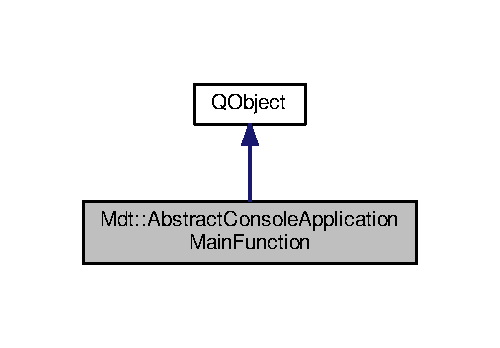
\includegraphics[width=240pt]{class_mdt_1_1_abstract_console_application_main_function__inherit__graph}
\end{center}
\end{figure}


Collaboration diagram for Mdt\+:\+:Abstract\+Console\+Application\+Main\+Function\+:\nopagebreak
\begin{figure}[H]
\begin{center}
\leavevmode
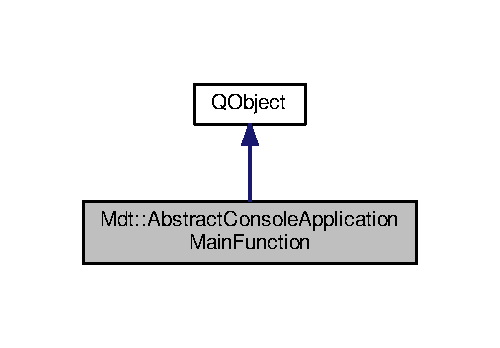
\includegraphics[width=240pt]{class_mdt_1_1_abstract_console_application_main_function__coll__graph}
\end{center}
\end{figure}
\subsection*{Public Slots}
\begin{DoxyCompactItemize}
\item 
virtual void \hyperlink{class_mdt_1_1_abstract_console_application_main_function_a7f00b12d06e341d037cd1a69632b2ac2}{about\+To\+Quit} ()
\begin{DoxyCompactList}\small\item\em Cleanup code. \end{DoxyCompactList}\end{DoxyCompactItemize}
\subsection*{Public Member Functions}
\begin{DoxyCompactItemize}
\item 
\hyperlink{class_mdt_1_1_abstract_console_application_main_function_aec80aaecedd4a2d6696878b96cfc9b40}{Abstract\+Console\+Application\+Main\+Function} (\hyperlink{class_q_object}{Q\+Object} $\ast$parent=nullptr)
\begin{DoxyCompactList}\small\item\em Constructor. \end{DoxyCompactList}\item 
virtual int \hyperlink{class_mdt_1_1_abstract_console_application_main_function_a34213b6ac2188b3620f5c2f5ce4ee287}{run\+Main} ()=0
\begin{DoxyCompactList}\small\item\em main function implementation \end{DoxyCompactList}\end{DoxyCompactItemize}
\subsection*{Static Public Member Functions}
\begin{DoxyCompactItemize}
\item 
static Q\+String\+List \hyperlink{class_mdt_1_1_abstract_console_application_main_function_a4bfe1909139f3c30b03797f7778290fb}{get\+Arguments} ()
\begin{DoxyCompactList}\small\item\em Returns the list of command-\/line arguments. \end{DoxyCompactList}\end{DoxyCompactItemize}


\subsection{Detailed Description}
Abstract base of a main function in Qt console application with a event loop. 

The class declaration My\+Main\+Function.\+h could look like\+: 
\begin{DoxyCode}
\textcolor{keyword}{class }MyMainFunction : \textcolor{keyword}{public} \hyperlink{class_mdt_1_1_abstract_console_application_main_function}{Mdt::AbstractConsoleApplicationMainFunction}
\{
 Q\_OBJECT

 \textcolor{keyword}{public}:

  \textcolor{keyword}{explicit} MyMainFunction(\hyperlink{class_q_object}{QObject}* parent = \textcolor{keyword}{nullptr});
  \textcolor{keywordtype}{int} \hyperlink{class_mdt_1_1_abstract_console_application_main_function_a34213b6ac2188b3620f5c2f5ce4ee287}{runMain}() \textcolor{keyword}{override};
\};
\end{DoxyCode}


Example of the implementation in My\+Main\+Function.\+cpp\+: 
\begin{DoxyCode}
\textcolor{keywordtype}{int} MyMainFunction::runMain()
\{
  qDebug() << \textcolor{stringliteral}{"My main ..."};
\}
\end{DoxyCode}


Finaly, in main.\+cpp\+: 
\begin{DoxyCode}
\hyperlink{class_q_core_application}{QCoreApplication} app(argc, argv);

\textcolor{comment}{// This will call runMain() once the event loop started}
MyMainFunction mainImpl;

\textcolor{keywordflow}{return} app.exec();
\end{DoxyCode}
 

Definition at line 62 of file Abstract\+Console\+Application\+Main\+Function.\+h.



\subsection{Constructor \& Destructor Documentation}
\index{Mdt\+::\+Abstract\+Console\+Application\+Main\+Function@{Mdt\+::\+Abstract\+Console\+Application\+Main\+Function}!Abstract\+Console\+Application\+Main\+Function@{Abstract\+Console\+Application\+Main\+Function}}
\index{Abstract\+Console\+Application\+Main\+Function@{Abstract\+Console\+Application\+Main\+Function}!Mdt\+::\+Abstract\+Console\+Application\+Main\+Function@{Mdt\+::\+Abstract\+Console\+Application\+Main\+Function}}
\subsubsection[{\texorpdfstring{Abstract\+Console\+Application\+Main\+Function(\+Q\+Object $\ast$parent=nullptr)}{AbstractConsoleApplicationMainFunction(QObject *parent=nullptr)}}]{\setlength{\rightskip}{0pt plus 5cm}Mdt\+::\+Abstract\+Console\+Application\+Main\+Function\+::\+Abstract\+Console\+Application\+Main\+Function (
\begin{DoxyParamCaption}
\item[{{\bf Q\+Object} $\ast$}]{parent = {\ttfamily nullptr}}
\end{DoxyParamCaption}
)\hspace{0.3cm}{\ttfamily [explicit]}}\hypertarget{class_mdt_1_1_abstract_console_application_main_function_aec80aaecedd4a2d6696878b96cfc9b40}{}\label{class_mdt_1_1_abstract_console_application_main_function_aec80aaecedd4a2d6696878b96cfc9b40}


Constructor. 



Definition at line 27 of file Abstract\+Console\+Application\+Main\+Function.\+cpp.



\subsection{Member Function Documentation}
\index{Mdt\+::\+Abstract\+Console\+Application\+Main\+Function@{Mdt\+::\+Abstract\+Console\+Application\+Main\+Function}!about\+To\+Quit@{about\+To\+Quit}}
\index{about\+To\+Quit@{about\+To\+Quit}!Mdt\+::\+Abstract\+Console\+Application\+Main\+Function@{Mdt\+::\+Abstract\+Console\+Application\+Main\+Function}}
\subsubsection[{\texorpdfstring{about\+To\+Quit}{aboutToQuit}}]{\setlength{\rightskip}{0pt plus 5cm}void Mdt\+::\+Abstract\+Console\+Application\+Main\+Function\+::about\+To\+Quit (
\begin{DoxyParamCaption}
{}
\end{DoxyParamCaption}
)\hspace{0.3cm}{\ttfamily [virtual]}, {\ttfamily [slot]}}\hypertarget{class_mdt_1_1_abstract_console_application_main_function_a7f00b12d06e341d037cd1a69632b2ac2}{}\label{class_mdt_1_1_abstract_console_application_main_function_a7f00b12d06e341d037cd1a69632b2ac2}


Cleanup code. 

If some cleanup has to be done before the application exists, this function can be implemented. See \hyperlink{class_q_core_application}{Q\+Core\+Application} documentation to know why this is a recommanded way to do cleanup.

This default implementation does nothing. 

Definition at line 41 of file Abstract\+Console\+Application\+Main\+Function.\+cpp.

\index{Mdt\+::\+Abstract\+Console\+Application\+Main\+Function@{Mdt\+::\+Abstract\+Console\+Application\+Main\+Function}!get\+Arguments@{get\+Arguments}}
\index{get\+Arguments@{get\+Arguments}!Mdt\+::\+Abstract\+Console\+Application\+Main\+Function@{Mdt\+::\+Abstract\+Console\+Application\+Main\+Function}}
\subsubsection[{\texorpdfstring{get\+Arguments()}{getArguments()}}]{\setlength{\rightskip}{0pt plus 5cm}Q\+String\+List Mdt\+::\+Abstract\+Console\+Application\+Main\+Function\+::get\+Arguments (
\begin{DoxyParamCaption}
{}
\end{DoxyParamCaption}
)\hspace{0.3cm}{\ttfamily [static]}}\hypertarget{class_mdt_1_1_abstract_console_application_main_function_a4bfe1909139f3c30b03797f7778290fb}{}\label{class_mdt_1_1_abstract_console_application_main_function_a4bfe1909139f3c30b03797f7778290fb}


Returns the list of command-\/line arguments. 

Returns Q\+Core\+Application\+::arguments(). As stated in \hyperlink{class_q_core_application}{Q\+Core\+Application} documentation, this method is slow, so the result should be stored in a variable if accessed many times (this is wy it is prefixed with get here)

\begin{DoxyPrecond}{Precondition}
A instance of a \hyperlink{class_q_core_application}{Q\+Core\+Application} (or one of its derivate) must exist. 
\end{DoxyPrecond}


Definition at line 34 of file Abstract\+Console\+Application\+Main\+Function.\+cpp.

\index{Mdt\+::\+Abstract\+Console\+Application\+Main\+Function@{Mdt\+::\+Abstract\+Console\+Application\+Main\+Function}!run\+Main@{run\+Main}}
\index{run\+Main@{run\+Main}!Mdt\+::\+Abstract\+Console\+Application\+Main\+Function@{Mdt\+::\+Abstract\+Console\+Application\+Main\+Function}}
\subsubsection[{\texorpdfstring{run\+Main()=0}{runMain()=0}}]{\setlength{\rightskip}{0pt plus 5cm}virtual int Mdt\+::\+Abstract\+Console\+Application\+Main\+Function\+::run\+Main (
\begin{DoxyParamCaption}
{}
\end{DoxyParamCaption}
)\hspace{0.3cm}{\ttfamily [pure virtual]}}\hypertarget{class_mdt_1_1_abstract_console_application_main_function_a34213b6ac2188b3620f5c2f5ce4ee287}{}\label{class_mdt_1_1_abstract_console_application_main_function_a34213b6ac2188b3620f5c2f5ce4ee287}


main function implementation 



The documentation for this class was generated from the following files\+:\begin{DoxyCompactItemize}
\item 
libs/\+Application\+\_\+\+Core/src/\+Mdt/Abstract\+Console\+Application\+Main\+Function.\+h\item 
libs/\+Application\+\_\+\+Core/src/\+Mdt/Abstract\+Console\+Application\+Main\+Function.\+cpp\end{DoxyCompactItemize}

\hypertarget{class_mdt_1_1_application}{}\section{Mdt\+:\+:Application Class Reference}
\label{class_mdt_1_1_application}\index{Mdt\+::\+Application@{Mdt\+::\+Application}}


\hyperlink{class_mdt_1_1_application}{Application} adds some helper for application initialization.  




{\ttfamily \#include $<$Application.\+h$>$}



Inheritance diagram for Mdt\+:\+:Application\+:\nopagebreak
\begin{figure}[H]
\begin{center}
\leavevmode
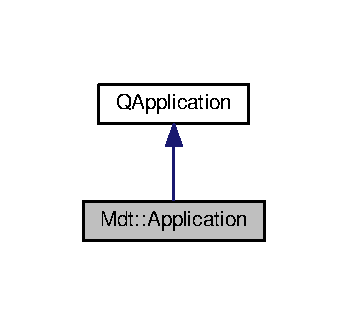
\includegraphics[width=167pt]{class_mdt_1_1_application__inherit__graph}
\end{center}
\end{figure}


Collaboration diagram for Mdt\+:\+:Application\+:\nopagebreak
\begin{figure}[H]
\begin{center}
\leavevmode
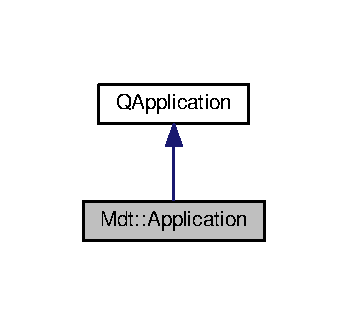
\includegraphics[width=167pt]{class_mdt_1_1_application__coll__graph}
\end{center}
\end{figure}
\subsection*{Public Member Functions}
\begin{DoxyCompactItemize}
\item 
\hyperlink{class_mdt_1_1_application_a5038a26f5618eba0c6f8c51e7eca76dd}{Application} (int \&argc, char $\ast$$\ast$argv)
\begin{DoxyCompactList}\small\item\em Creates a \hyperlink{class_mdt_1_1_application}{Application} object. \end{DoxyCompactList}\item 
\hyperlink{class_mdt_1_1_application_a24456c7eb1e79fa5c73459f1c64f7e84}{$\sim$\+Application} ()
\begin{DoxyCompactList}\small\item\em Destructor. \end{DoxyCompactList}\item 
{\bfseries Application} (const \hyperlink{class_mdt_1_1_application}{Application} \&)=delete\hypertarget{class_mdt_1_1_application_a5c17bc0f9eeda52a18f13e797cdc49e7}{}\label{class_mdt_1_1_application_a5c17bc0f9eeda52a18f13e797cdc49e7}

\item 
\hyperlink{class_mdt_1_1_application}{Application} \& {\bfseries operator=} (const \hyperlink{class_mdt_1_1_application}{Application} \&)=delete\hypertarget{class_mdt_1_1_application_a3b0046f08873c3f74357ed92e39433da}{}\label{class_mdt_1_1_application_a3b0046f08873c3f74357ed92e39433da}

\item 
{\bfseries Application} (\hyperlink{class_mdt_1_1_application}{Application} \&\&)=delete\hypertarget{class_mdt_1_1_application_a70f78a5e7bbf97c58530b59cc5fa041e}{}\label{class_mdt_1_1_application_a70f78a5e7bbf97c58530b59cc5fa041e}

\item 
\hyperlink{class_mdt_1_1_application}{Application} \& {\bfseries operator=} (\hyperlink{class_mdt_1_1_application}{Application} \&\&)=delete\hypertarget{class_mdt_1_1_application_a61d3d984d0caa80a0bbbaadab4fd5c9c}{}\label{class_mdt_1_1_application_a61d3d984d0caa80a0bbbaadab4fd5c9c}

\item 
void \hyperlink{class_mdt_1_1_application_ab16dbd8818c2bf6e0c82208b3f5c829b}{enable\+File\+Logging} ()
\begin{DoxyCompactList}\small\item\em Enable file logging. \end{DoxyCompactList}\item 
Q\+String \hyperlink{class_mdt_1_1_application_a8531dd25ea6a6dba62f1bcaea89723a7}{log\+File\+Path} ()
\begin{DoxyCompactList}\small\item\em Get the path to the log file. \end{DoxyCompactList}\item 
void \hyperlink{class_mdt_1_1_application_a055baa70e5c4f78c2472ca39755aa111}{debug\+Environment} ()
\begin{DoxyCompactList}\small\item\em Debug environment. \end{DoxyCompactList}\end{DoxyCompactItemize}
\subsection*{Static Public Member Functions}
\begin{DoxyCompactItemize}
\item 
static Q\+String \hyperlink{class_mdt_1_1_application_ac78756faf1b2c36c4f4f11334c3f8516}{cache\+Directory\+Path} ()
\begin{DoxyCompactList}\small\item\em Get path to the cache directory. \end{DoxyCompactList}\item 
static Q\+String \hyperlink{class_mdt_1_1_application_ac2842431a2fa3fb63345d99e8943baa0}{qt\+Version} ()
\begin{DoxyCompactList}\small\item\em Get Qt library version. \end{DoxyCompactList}\item 
static Q\+String \hyperlink{class_mdt_1_1_application_a818de2899b8aad3623e4fe46245f82e6}{mdt\+Version} ()
\begin{DoxyCompactList}\small\item\em Get \hyperlink{namespace_mdt}{Mdt} library version. \end{DoxyCompactList}\end{DoxyCompactItemize}


\subsection{Detailed Description}
\hyperlink{class_mdt_1_1_application}{Application} adds some helper for application initialization. 

\begin{DoxySeeAlso}{See also}
\hyperlink{class_q_application}{Q\+Application} 
\end{DoxySeeAlso}


Definition at line 36 of file Application.\+h.



\subsection{Constructor \& Destructor Documentation}
\index{Mdt\+::\+Application@{Mdt\+::\+Application}!Application@{Application}}
\index{Application@{Application}!Mdt\+::\+Application@{Mdt\+::\+Application}}
\subsubsection[{\texorpdfstring{Application(int \&argc, char $\ast$$\ast$argv)}{Application(int &argc, char **argv)}}]{\setlength{\rightskip}{0pt plus 5cm}Mdt\+::\+Application\+::\+Application (
\begin{DoxyParamCaption}
\item[{int \&}]{argc, }
\item[{char $\ast$$\ast$}]{argv}
\end{DoxyParamCaption}
)}\hypertarget{class_mdt_1_1_application_a5038a26f5618eba0c6f8c51e7eca76dd}{}\label{class_mdt_1_1_application_a5038a26f5618eba0c6f8c51e7eca76dd}


Creates a \hyperlink{class_mdt_1_1_application}{Application} object. 



Definition at line 26 of file Application.\+cpp.

\index{Mdt\+::\+Application@{Mdt\+::\+Application}!````~Application@{$\sim$\+Application}}
\index{````~Application@{$\sim$\+Application}!Mdt\+::\+Application@{Mdt\+::\+Application}}
\subsubsection[{\texorpdfstring{$\sim$\+Application()}{~Application()}}]{\setlength{\rightskip}{0pt plus 5cm}Mdt\+::\+Application\+::$\sim$\+Application (
\begin{DoxyParamCaption}
{}
\end{DoxyParamCaption}
)}\hypertarget{class_mdt_1_1_application_a24456c7eb1e79fa5c73459f1c64f7e84}{}\label{class_mdt_1_1_application_a24456c7eb1e79fa5c73459f1c64f7e84}


Destructor. 



Definition at line 32 of file Application.\+cpp.



\subsection{Member Function Documentation}
\index{Mdt\+::\+Application@{Mdt\+::\+Application}!cache\+Directory\+Path@{cache\+Directory\+Path}}
\index{cache\+Directory\+Path@{cache\+Directory\+Path}!Mdt\+::\+Application@{Mdt\+::\+Application}}
\subsubsection[{\texorpdfstring{cache\+Directory\+Path()}{cacheDirectoryPath()}}]{\setlength{\rightskip}{0pt plus 5cm}Q\+String Mdt\+::\+Application\+::cache\+Directory\+Path (
\begin{DoxyParamCaption}
{}
\end{DoxyParamCaption}
)\hspace{0.3cm}{\ttfamily [static]}}\hypertarget{class_mdt_1_1_application_ac78756faf1b2c36c4f4f11334c3f8516}{}\label{class_mdt_1_1_application_ac78756faf1b2c36c4f4f11334c3f8516}


Get path to the cache directory. 

Returns \hyperlink{class_mdt_1_1_standard_paths_a2ca803e5a6b9fb2a4808968becfb86de}{Standard\+Paths\+::cache\+Directory\+Path()} 

Definition at line 46 of file Application.\+cpp.

\index{Mdt\+::\+Application@{Mdt\+::\+Application}!debug\+Environment@{debug\+Environment}}
\index{debug\+Environment@{debug\+Environment}!Mdt\+::\+Application@{Mdt\+::\+Application}}
\subsubsection[{\texorpdfstring{debug\+Environment()}{debugEnvironment()}}]{\setlength{\rightskip}{0pt plus 5cm}void Mdt\+::\+Application\+::debug\+Environment (
\begin{DoxyParamCaption}
{}
\end{DoxyParamCaption}
)}\hypertarget{class_mdt_1_1_application_a055baa70e5c4f78c2472ca39755aa111}{}\label{class_mdt_1_1_application_a055baa70e5c4f78c2472ca39755aa111}


Debug environment. 

Will print various informations, like libraries versions, paths to some directories, etc.. to the console. 

Definition at line 61 of file Application.\+cpp.

\index{Mdt\+::\+Application@{Mdt\+::\+Application}!enable\+File\+Logging@{enable\+File\+Logging}}
\index{enable\+File\+Logging@{enable\+File\+Logging}!Mdt\+::\+Application@{Mdt\+::\+Application}}
\subsubsection[{\texorpdfstring{enable\+File\+Logging()}{enableFileLogging()}}]{\setlength{\rightskip}{0pt plus 5cm}void Mdt\+::\+Application\+::enable\+File\+Logging (
\begin{DoxyParamCaption}
{}
\end{DoxyParamCaption}
)}\hypertarget{class_mdt_1_1_application_ab16dbd8818c2bf6e0c82208b3f5c829b}{}\label{class_mdt_1_1_application_ab16dbd8818c2bf6e0c82208b3f5c829b}


Enable file logging. 

After file logging was enabled, errors that are committed using \hyperlink{class_mdt_1_1_error_a1b4a57bd4177d2985abd62b6b49a43f8}{Mdt\+::\+Error\+::commit()} are added to the log file {\itshape \hyperlink{class_mdt_1_1_application_a8531dd25ea6a6dba62f1bcaea89723a7}{log\+File\+Path()}} . 

Definition at line 36 of file Application.\+cpp.

\index{Mdt\+::\+Application@{Mdt\+::\+Application}!log\+File\+Path@{log\+File\+Path}}
\index{log\+File\+Path@{log\+File\+Path}!Mdt\+::\+Application@{Mdt\+::\+Application}}
\subsubsection[{\texorpdfstring{log\+File\+Path()}{logFilePath()}}]{\setlength{\rightskip}{0pt plus 5cm}Q\+String Mdt\+::\+Application\+::log\+File\+Path (
\begin{DoxyParamCaption}
{}
\end{DoxyParamCaption}
)}\hypertarget{class_mdt_1_1_application_a8531dd25ea6a6dba62f1bcaea89723a7}{}\label{class_mdt_1_1_application_a8531dd25ea6a6dba62f1bcaea89723a7}


Get the path to the log file. 



Definition at line 41 of file Application.\+cpp.

\index{Mdt\+::\+Application@{Mdt\+::\+Application}!mdt\+Version@{mdt\+Version}}
\index{mdt\+Version@{mdt\+Version}!Mdt\+::\+Application@{Mdt\+::\+Application}}
\subsubsection[{\texorpdfstring{mdt\+Version()}{mdtVersion()}}]{\setlength{\rightskip}{0pt plus 5cm}Q\+String Mdt\+::\+Application\+::mdt\+Version (
\begin{DoxyParamCaption}
{}
\end{DoxyParamCaption}
)\hspace{0.3cm}{\ttfamily [static]}}\hypertarget{class_mdt_1_1_application_a818de2899b8aad3623e4fe46245f82e6}{}\label{class_mdt_1_1_application_a818de2899b8aad3623e4fe46245f82e6}


Get \hyperlink{namespace_mdt}{Mdt} library version. 



Definition at line 56 of file Application.\+cpp.

\index{Mdt\+::\+Application@{Mdt\+::\+Application}!qt\+Version@{qt\+Version}}
\index{qt\+Version@{qt\+Version}!Mdt\+::\+Application@{Mdt\+::\+Application}}
\subsubsection[{\texorpdfstring{qt\+Version()}{qtVersion()}}]{\setlength{\rightskip}{0pt plus 5cm}Q\+String Mdt\+::\+Application\+::qt\+Version (
\begin{DoxyParamCaption}
{}
\end{DoxyParamCaption}
)\hspace{0.3cm}{\ttfamily [static]}}\hypertarget{class_mdt_1_1_application_ac2842431a2fa3fb63345d99e8943baa0}{}\label{class_mdt_1_1_application_ac2842431a2fa3fb63345d99e8943baa0}


Get Qt library version. 



Definition at line 51 of file Application.\+cpp.



The documentation for this class was generated from the following files\+:\begin{DoxyCompactItemize}
\item 
libs/\+Application\+\_\+\+Widgets/src/\+Mdt/Application.\+h\item 
libs/\+Application\+\_\+\+Widgets/src/\+Mdt/Application.\+cpp\end{DoxyCompactItemize}

\hypertarget{class_mdt_1_1_application_impl}{}\section{Mdt\+:\+:Application\+Impl Class Reference}
\label{class_mdt_1_1_application_impl}\index{Mdt\+::\+Application\+Impl@{Mdt\+::\+Application\+Impl}}


Implementation for \hyperlink{class_mdt_1_1_application}{Application} and related classes.  




{\ttfamily \#include $<$Application\+Impl.\+h$>$}



Inheritance diagram for Mdt\+:\+:Application\+Impl\+:
\nopagebreak
\begin{figure}[H]
\begin{center}
\leavevmode
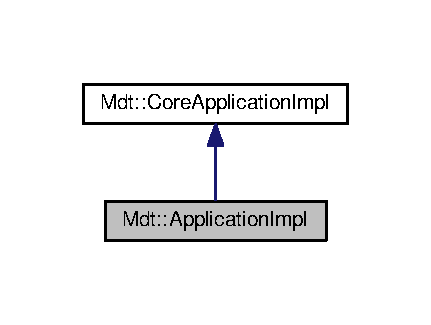
\includegraphics[width=207pt]{class_mdt_1_1_application_impl__inherit__graph}
\end{center}
\end{figure}


Collaboration diagram for Mdt\+:\+:Application\+Impl\+:
\nopagebreak
\begin{figure}[H]
\begin{center}
\leavevmode
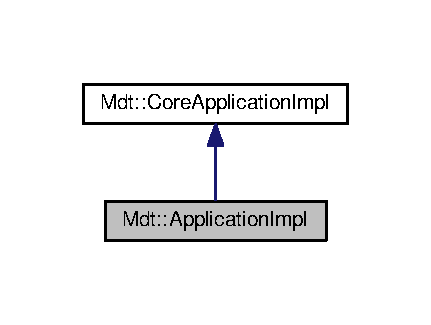
\includegraphics[width=207pt]{class_mdt_1_1_application_impl__coll__graph}
\end{center}
\end{figure}
\subsection*{Public Member Functions}
\begin{DoxyCompactItemize}
\item 
\hyperlink{class_mdt_1_1_application_impl_a512c94eac0af0b0fb9ecd76af49fa473}{Application\+Impl} ()=default
\begin{DoxyCompactList}\small\item\em Constructor. \end{DoxyCompactList}\item 
\hyperlink{class_mdt_1_1_application_impl_aacb32f587d7f8da64472026e8cf28f3c}{$\sim$\+Application\+Impl} ()=default
\begin{DoxyCompactList}\small\item\em Destructor. \end{DoxyCompactList}\item 
{\bfseries Application\+Impl} (const \hyperlink{class_mdt_1_1_application_impl}{Application\+Impl} \&)=delete\hypertarget{class_mdt_1_1_application_impl_a3b52a0b38ddb8032cdf38e518281fa47}{}\label{class_mdt_1_1_application_impl_a3b52a0b38ddb8032cdf38e518281fa47}

\item 
\hyperlink{class_mdt_1_1_application_impl}{Application\+Impl} \& {\bfseries operator=} (const \hyperlink{class_mdt_1_1_application_impl}{Application\+Impl} \&)=delete\hypertarget{class_mdt_1_1_application_impl_a00b1d241ed42d182046c1f24732d17b2}{}\label{class_mdt_1_1_application_impl_a00b1d241ed42d182046c1f24732d17b2}

\item 
{\bfseries Application\+Impl} (\hyperlink{class_mdt_1_1_application_impl}{Application\+Impl} \&\&)=delete\hypertarget{class_mdt_1_1_application_impl_a462a167732205be4879aaa897afd644e}{}\label{class_mdt_1_1_application_impl_a462a167732205be4879aaa897afd644e}

\item 
\hyperlink{class_mdt_1_1_application_impl}{Application\+Impl} \& {\bfseries operator=} (\hyperlink{class_mdt_1_1_application_impl}{Application\+Impl} \&\&)=delete\hypertarget{class_mdt_1_1_application_impl_adfdc2f1d0a9145df7431ec8a93a4ef6a}{}\label{class_mdt_1_1_application_impl_adfdc2f1d0a9145df7431ec8a93a4ef6a}

\item 
Q\+String\+List \hyperlink{class_mdt_1_1_application_impl_a50deab1146432008cfed699c817dd315}{environment\+Entries} ()
\begin{DoxyCompactList}\small\item\em Get environment entries. \end{DoxyCompactList}\end{DoxyCompactItemize}
\subsection*{Additional Inherited Members}


\subsection{Detailed Description}
Implementation for \hyperlink{class_mdt_1_1_application}{Application} and related classes. 

Definition at line 30 of file Application\+Impl.\+h.



\subsection{Constructor \& Destructor Documentation}
\index{Mdt\+::\+Application\+Impl@{Mdt\+::\+Application\+Impl}!Application\+Impl@{Application\+Impl}}
\index{Application\+Impl@{Application\+Impl}!Mdt\+::\+Application\+Impl@{Mdt\+::\+Application\+Impl}}
\subsubsection[{\texorpdfstring{Application\+Impl()=default}{ApplicationImpl()=default}}]{\setlength{\rightskip}{0pt plus 5cm}Mdt\+::\+Application\+Impl\+::\+Application\+Impl (
\begin{DoxyParamCaption}
{}
\end{DoxyParamCaption}
)\hspace{0.3cm}{\ttfamily [default]}}\hypertarget{class_mdt_1_1_application_impl_a512c94eac0af0b0fb9ecd76af49fa473}{}\label{class_mdt_1_1_application_impl_a512c94eac0af0b0fb9ecd76af49fa473}


Constructor. 

\index{Mdt\+::\+Application\+Impl@{Mdt\+::\+Application\+Impl}!````~Application\+Impl@{$\sim$\+Application\+Impl}}
\index{````~Application\+Impl@{$\sim$\+Application\+Impl}!Mdt\+::\+Application\+Impl@{Mdt\+::\+Application\+Impl}}
\subsubsection[{\texorpdfstring{$\sim$\+Application\+Impl()=default}{~ApplicationImpl()=default}}]{\setlength{\rightskip}{0pt plus 5cm}Mdt\+::\+Application\+Impl\+::$\sim$\+Application\+Impl (
\begin{DoxyParamCaption}
{}
\end{DoxyParamCaption}
)\hspace{0.3cm}{\ttfamily [default]}}\hypertarget{class_mdt_1_1_application_impl_aacb32f587d7f8da64472026e8cf28f3c}{}\label{class_mdt_1_1_application_impl_aacb32f587d7f8da64472026e8cf28f3c}


Destructor. 



\subsection{Member Function Documentation}
\index{Mdt\+::\+Application\+Impl@{Mdt\+::\+Application\+Impl}!environment\+Entries@{environment\+Entries}}
\index{environment\+Entries@{environment\+Entries}!Mdt\+::\+Application\+Impl@{Mdt\+::\+Application\+Impl}}
\subsubsection[{\texorpdfstring{environment\+Entries()}{environmentEntries()}}]{\setlength{\rightskip}{0pt plus 5cm}Q\+String\+List Mdt\+::\+Application\+Impl\+::environment\+Entries (
\begin{DoxyParamCaption}
{}
\end{DoxyParamCaption}
)}\hypertarget{class_mdt_1_1_application_impl_a50deab1146432008cfed699c817dd315}{}\label{class_mdt_1_1_application_impl_a50deab1146432008cfed699c817dd315}


Get environment entries. 



Definition at line 28 of file Application\+Impl.\+cpp.



The documentation for this class was generated from the following files\+:\begin{DoxyCompactItemize}
\item 
libs/\+Application\+\_\+\+Widgets/src/\+Mdt/Application\+Impl.\+h\item 
libs/\+Application\+\_\+\+Widgets/src/\+Mdt/Application\+Impl.\+cpp\end{DoxyCompactItemize}

\hypertarget{class_mdt_1_1_error_logger_1_1_backend}{}\section{Mdt\+:\+:Error\+Logger\+:\+:Backend Class Reference}
\label{class_mdt_1_1_error_logger_1_1_backend}\index{Mdt\+::\+Error\+Logger\+::\+Backend@{Mdt\+::\+Error\+Logger\+::\+Backend}}


\hyperlink{class_mdt_1_1_error}{Error} \hyperlink{class_mdt_1_1_error_logger_1_1_logger}{Logger} backend.  




{\ttfamily \#include $<$Backend.\+h$>$}



Inheritance diagram for Mdt\+:\+:Error\+Logger\+:\+:Backend\+:
\nopagebreak
\begin{figure}[H]
\begin{center}
\leavevmode
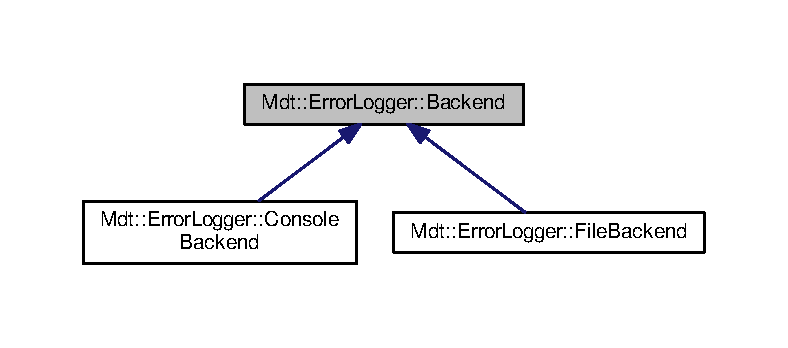
\includegraphics[width=350pt]{class_mdt_1_1_error_logger_1_1_backend__inherit__graph}
\end{center}
\end{figure}
\subsection*{Public Member Functions}
\begin{DoxyCompactItemize}
\item 
\hyperlink{class_mdt_1_1_error_logger_1_1_backend_acf0b4a7f061c638207bfdb172fc8015c}{Backend} ()
\begin{DoxyCompactList}\small\item\em Constructor. \end{DoxyCompactList}\item 
virtual \hyperlink{class_mdt_1_1_error_logger_1_1_backend_aba972e76fc4d6bb7665038cb8d1c88d7}{$\sim$\+Backend} ()
\begin{DoxyCompactList}\small\item\em Destructor. \end{DoxyCompactList}\item 
virtual void \hyperlink{class_mdt_1_1_error_logger_1_1_backend_acf37cfc576269934ca8ce04e3601058d}{log\+Error} (const \hyperlink{class_mdt_1_1_error}{Error} \&error)=0
\begin{DoxyCompactList}\small\item\em Log given error. \end{DoxyCompactList}\item 
{\bfseries Backend} (const \hyperlink{class_mdt_1_1_error_logger_1_1_backend}{Backend} \&)=delete\hypertarget{class_mdt_1_1_error_logger_1_1_backend_a7bb295be149f2205fe63554e1ba06f66}{}\label{class_mdt_1_1_error_logger_1_1_backend_a7bb295be149f2205fe63554e1ba06f66}

\item 
{\bfseries Backend} (\hyperlink{class_mdt_1_1_error_logger_1_1_backend}{Backend} \&\&)=delete\hypertarget{class_mdt_1_1_error_logger_1_1_backend_aba1ff6190a3b08ca93e8edd7917a7d25}{}\label{class_mdt_1_1_error_logger_1_1_backend_aba1ff6190a3b08ca93e8edd7917a7d25}

\item 
\hyperlink{class_mdt_1_1_error_logger_1_1_backend}{Backend} \& {\bfseries operator=} (const \hyperlink{class_mdt_1_1_error_logger_1_1_backend}{Backend} \&)=delete\hypertarget{class_mdt_1_1_error_logger_1_1_backend_a9400fcafaec1e9e07da2d31dcc842b92}{}\label{class_mdt_1_1_error_logger_1_1_backend_a9400fcafaec1e9e07da2d31dcc842b92}

\item 
\hyperlink{class_mdt_1_1_error_logger_1_1_backend}{Backend} \& {\bfseries operator=} (\hyperlink{class_mdt_1_1_error_logger_1_1_backend}{Backend} \&\&)=delete\hypertarget{class_mdt_1_1_error_logger_1_1_backend_ae0beab19d09a61f83eb5feed501a7562}{}\label{class_mdt_1_1_error_logger_1_1_backend_ae0beab19d09a61f83eb5feed501a7562}

\end{DoxyCompactItemize}
\subsection*{Static Protected Member Functions}
\begin{DoxyCompactItemize}
\item 
static Q\+String \hyperlink{class_mdt_1_1_error_logger_1_1_backend_a4a859ea87b93082e69791bcbd14c1f71}{tr} (const char $\ast$text)
\begin{DoxyCompactList}\small\item\em Calls Q\+Object\+::tr() \end{DoxyCompactList}\end{DoxyCompactItemize}


\subsection{Detailed Description}
\hyperlink{class_mdt_1_1_error}{Error} \hyperlink{class_mdt_1_1_error_logger_1_1_logger}{Logger} backend. 

This class is a interface to create a error logger backend that will be used by error \hyperlink{class_mdt_1_1_error_logger_1_1_logger}{Logger} to output errors.

Notice that \hyperlink{class_mdt_1_1_error_logger_1_1_logger}{Logger} executes from a non main thread, also take care that some functons must at least be reentrant. 

Definition at line 40 of file Backend.\+h.



\subsection{Constructor \& Destructor Documentation}
\index{Mdt\+::\+Error\+Logger\+::\+Backend@{Mdt\+::\+Error\+Logger\+::\+Backend}!Backend@{Backend}}
\index{Backend@{Backend}!Mdt\+::\+Error\+Logger\+::\+Backend@{Mdt\+::\+Error\+Logger\+::\+Backend}}
\subsubsection[{\texorpdfstring{Backend()}{Backend()}}]{\setlength{\rightskip}{0pt plus 5cm}Mdt\+::\+Error\+Logger\+::\+Backend\+::\+Backend (
\begin{DoxyParamCaption}
{}
\end{DoxyParamCaption}
)\hspace{0.3cm}{\ttfamily [inline]}}\hypertarget{class_mdt_1_1_error_logger_1_1_backend_acf0b4a7f061c638207bfdb172fc8015c}{}\label{class_mdt_1_1_error_logger_1_1_backend_acf0b4a7f061c638207bfdb172fc8015c}


Constructor. 



Definition at line 46 of file Backend.\+h.



Referenced by $\sim$\+Backend().

\index{Mdt\+::\+Error\+Logger\+::\+Backend@{Mdt\+::\+Error\+Logger\+::\+Backend}!````~Backend@{$\sim$\+Backend}}
\index{````~Backend@{$\sim$\+Backend}!Mdt\+::\+Error\+Logger\+::\+Backend@{Mdt\+::\+Error\+Logger\+::\+Backend}}
\subsubsection[{\texorpdfstring{$\sim$\+Backend()}{~Backend()}}]{\setlength{\rightskip}{0pt plus 5cm}virtual Mdt\+::\+Error\+Logger\+::\+Backend\+::$\sim$\+Backend (
\begin{DoxyParamCaption}
{}
\end{DoxyParamCaption}
)\hspace{0.3cm}{\ttfamily [inline]}, {\ttfamily [virtual]}}\hypertarget{class_mdt_1_1_error_logger_1_1_backend_aba972e76fc4d6bb7665038cb8d1c88d7}{}\label{class_mdt_1_1_error_logger_1_1_backend_aba972e76fc4d6bb7665038cb8d1c88d7}


Destructor. 



Definition at line 50 of file Backend.\+h.



References Backend(), log\+Error(), and tr().



\subsection{Member Function Documentation}
\index{Mdt\+::\+Error\+Logger\+::\+Backend@{Mdt\+::\+Error\+Logger\+::\+Backend}!log\+Error@{log\+Error}}
\index{log\+Error@{log\+Error}!Mdt\+::\+Error\+Logger\+::\+Backend@{Mdt\+::\+Error\+Logger\+::\+Backend}}
\subsubsection[{\texorpdfstring{log\+Error(const Error \&error)=0}{logError(const Error &error)=0}}]{\setlength{\rightskip}{0pt plus 5cm}virtual void Mdt\+::\+Error\+Logger\+::\+Backend\+::log\+Error (
\begin{DoxyParamCaption}
\item[{const {\bf Error} \&}]{error}
\end{DoxyParamCaption}
)\hspace{0.3cm}{\ttfamily [pure virtual]}}\hypertarget{class_mdt_1_1_error_logger_1_1_backend_acf37cfc576269934ca8ce04e3601058d}{}\label{class_mdt_1_1_error_logger_1_1_backend_acf37cfc576269934ca8ce04e3601058d}


Log given error. 

This function must be reentrant, because its called from \hyperlink{class_mdt_1_1_error_logger_1_1_logger}{Logger} thread (witch is not the main thread). 

Implemented in \hyperlink{class_mdt_1_1_error_logger_1_1_file_backend_a31b8314d523a491b5441276122daed87}{Mdt\+::\+Error\+Logger\+::\+File\+Backend}, and \hyperlink{class_mdt_1_1_error_logger_1_1_console_backend_a2d30700dd6a91c244d68bd3670fdbc33}{Mdt\+::\+Error\+Logger\+::\+Console\+Backend}.



Referenced by $\sim$\+Backend().

\index{Mdt\+::\+Error\+Logger\+::\+Backend@{Mdt\+::\+Error\+Logger\+::\+Backend}!tr@{tr}}
\index{tr@{tr}!Mdt\+::\+Error\+Logger\+::\+Backend@{Mdt\+::\+Error\+Logger\+::\+Backend}}
\subsubsection[{\texorpdfstring{tr(const char $\ast$text)}{tr(const char *text)}}]{\setlength{\rightskip}{0pt plus 5cm}Q\+String Mdt\+::\+Error\+Logger\+::\+Backend\+::tr (
\begin{DoxyParamCaption}
\item[{const char $\ast$}]{text}
\end{DoxyParamCaption}
)\hspace{0.3cm}{\ttfamily [static]}, {\ttfamily [protected]}}\hypertarget{class_mdt_1_1_error_logger_1_1_backend_a4a859ea87b93082e69791bcbd14c1f71}{}\label{class_mdt_1_1_error_logger_1_1_backend_a4a859ea87b93082e69791bcbd14c1f71}


Calls Q\+Object\+::tr() 



Definition at line 24 of file Backend.\+cpp.



Referenced by Mdt\+::\+Error\+Logger\+::\+Console\+Backend\+::log\+Error(), Mdt\+::\+Error\+Logger\+::\+File\+Backend\+::log\+Error(), Mdt\+::\+Error\+Logger\+::\+File\+Backend\+::set\+Log\+File\+Path(), and $\sim$\+Backend().



The documentation for this class was generated from the following files\+:\begin{DoxyCompactItemize}
\item 
libs/\+Error\+\_\+\+Core/src/\+Mdt/\+Error\+Logger/Backend.\+h\item 
libs/\+Error\+\_\+\+Core/src/\+Mdt/\+Error\+Logger/Backend.\+cpp\end{DoxyCompactItemize}

\hypertarget{class_mdt_1_1_deploy_utils_1_1_binary_dependencies}{}\section{Mdt\+:\+:Deploy\+Utils\+:\+:Binary\+Dependencies Class Reference}
\label{class_mdt_1_1_deploy_utils_1_1_binary_dependencies}\index{Mdt\+::\+Deploy\+Utils\+::\+Binary\+Dependencies@{Mdt\+::\+Deploy\+Utils\+::\+Binary\+Dependencies}}


Find dependencies for a executable or a library.  




{\ttfamily \#include $<$Binary\+Dependencies.\+h$>$}



Inheritance diagram for Mdt\+:\+:Deploy\+Utils\+:\+:Binary\+Dependencies\+:
\nopagebreak
\begin{figure}[H]
\begin{center}
\leavevmode
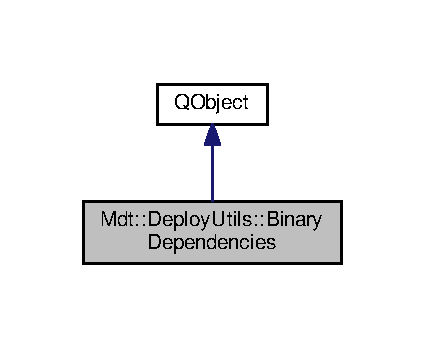
\includegraphics[width=204pt]{class_mdt_1_1_deploy_utils_1_1_binary_dependencies__inherit__graph}
\end{center}
\end{figure}


Collaboration diagram for Mdt\+:\+:Deploy\+Utils\+:\+:Binary\+Dependencies\+:
\nopagebreak
\begin{figure}[H]
\begin{center}
\leavevmode
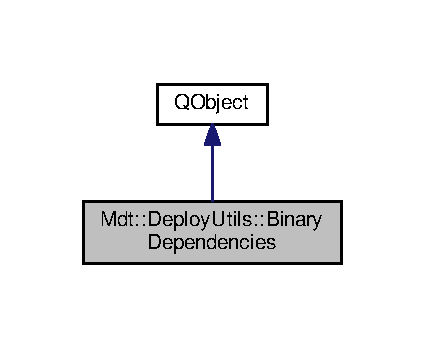
\includegraphics[width=204pt]{class_mdt_1_1_deploy_utils_1_1_binary_dependencies__coll__graph}
\end{center}
\end{figure}
\subsection*{Public Member Functions}
\begin{DoxyCompactItemize}
\item 
\hyperlink{class_mdt_1_1_deploy_utils_1_1_binary_dependencies_aa4decd7ce7db7292738f6d300445e6b0}{Binary\+Dependencies} (\hyperlink{class_q_object}{Q\+Object} $\ast$parent=nullptr)
\begin{DoxyCompactList}\small\item\em Constructor. \end{DoxyCompactList}\item 
\hyperlink{class_mdt_1_1_deploy_utils_1_1_binary_dependencies_a6bb36d0457ccd40462edb70cefc25bba}{$\sim$\+Binary\+Dependencies} ()
\begin{DoxyCompactList}\small\item\em Destructor. \end{DoxyCompactList}\item 
bool \hyperlink{class_mdt_1_1_deploy_utils_1_1_binary_dependencies_ab57081aeb3581d58f5677129ce564013}{find\+Dependencies} (const Q\+String \&binary\+File\+Path, const \hyperlink{class_mdt_1_1_deploy_utils_1_1_path_list}{Path\+List} \&search\+First\+Path\+Prefix\+List)
\begin{DoxyCompactList}\small\item\em Find dependencies for a executable or a library. \end{DoxyCompactList}\item 
bool \hyperlink{class_mdt_1_1_deploy_utils_1_1_binary_dependencies_a6b2116711ce9bbc3b3523eac16af28ec}{find\+Dependencies} (const Q\+String\+List \&binaries\+File\+Paths, const \hyperlink{class_mdt_1_1_deploy_utils_1_1_path_list}{Path\+List} \&search\+First\+Path\+Prefix\+List)
\begin{DoxyCompactList}\small\item\em Find dependencies for a list of executables and/or libraries. \end{DoxyCompactList}\item 
bool \hyperlink{class_mdt_1_1_deploy_utils_1_1_binary_dependencies_a99b12cd9e28d27d33d416a51e116f54e}{find\+Dependencies} (const \hyperlink{class_mdt_1_1_deploy_utils_1_1_library_info_list}{Library\+Info\+List} \&libraries, const \hyperlink{class_mdt_1_1_deploy_utils_1_1_path_list}{Path\+List} \&search\+First\+Path\+Prefix\+List)
\begin{DoxyCompactList}\small\item\em Find dependencies for a lits of libraries. \end{DoxyCompactList}\item 
\hyperlink{class_mdt_1_1_deploy_utils_1_1_library_info_list}{Library\+Info\+List} \hyperlink{class_mdt_1_1_deploy_utils_1_1_binary_dependencies_a53e68f923a4c13493eba8990eaf6b5ef}{dependencies} () const 
\begin{DoxyCompactList}\small\item\em Get dependencies. \end{DoxyCompactList}\item 
\hyperlink{class_mdt_1_1_error}{Mdt\+::\+Error} \hyperlink{class_mdt_1_1_deploy_utils_1_1_binary_dependencies_ada341a03a0f42c02cf0d23f82e21f58e}{last\+Error} () const 
\begin{DoxyCompactList}\small\item\em Get last error. \end{DoxyCompactList}\end{DoxyCompactItemize}


\subsection{Detailed Description}
Find dependencies for a executable or a library. 

Definition at line 40 of file Binary\+Dependencies.\+h.



\subsection{Constructor \& Destructor Documentation}
\index{Mdt\+::\+Deploy\+Utils\+::\+Binary\+Dependencies@{Mdt\+::\+Deploy\+Utils\+::\+Binary\+Dependencies}!Binary\+Dependencies@{Binary\+Dependencies}}
\index{Binary\+Dependencies@{Binary\+Dependencies}!Mdt\+::\+Deploy\+Utils\+::\+Binary\+Dependencies@{Mdt\+::\+Deploy\+Utils\+::\+Binary\+Dependencies}}
\subsubsection[{\texorpdfstring{Binary\+Dependencies(\+Q\+Object $\ast$parent=nullptr)}{BinaryDependencies(QObject *parent=nullptr)}}]{\setlength{\rightskip}{0pt plus 5cm}Mdt\+::\+Deploy\+Utils\+::\+Binary\+Dependencies\+::\+Binary\+Dependencies (
\begin{DoxyParamCaption}
\item[{{\bf Q\+Object} $\ast$}]{parent = {\ttfamily nullptr}}
\end{DoxyParamCaption}
)}\hypertarget{class_mdt_1_1_deploy_utils_1_1_binary_dependencies_aa4decd7ce7db7292738f6d300445e6b0}{}\label{class_mdt_1_1_deploy_utils_1_1_binary_dependencies_aa4decd7ce7db7292738f6d300445e6b0}


Constructor. 



Definition at line 35 of file Binary\+Dependencies.\+cpp.

\index{Mdt\+::\+Deploy\+Utils\+::\+Binary\+Dependencies@{Mdt\+::\+Deploy\+Utils\+::\+Binary\+Dependencies}!````~Binary\+Dependencies@{$\sim$\+Binary\+Dependencies}}
\index{````~Binary\+Dependencies@{$\sim$\+Binary\+Dependencies}!Mdt\+::\+Deploy\+Utils\+::\+Binary\+Dependencies@{Mdt\+::\+Deploy\+Utils\+::\+Binary\+Dependencies}}
\subsubsection[{\texorpdfstring{$\sim$\+Binary\+Dependencies()}{~BinaryDependencies()}}]{\setlength{\rightskip}{0pt plus 5cm}Mdt\+::\+Deploy\+Utils\+::\+Binary\+Dependencies\+::$\sim$\+Binary\+Dependencies (
\begin{DoxyParamCaption}
{}
\end{DoxyParamCaption}
)}\hypertarget{class_mdt_1_1_deploy_utils_1_1_binary_dependencies_a6bb36d0457ccd40462edb70cefc25bba}{}\label{class_mdt_1_1_deploy_utils_1_1_binary_dependencies_a6bb36d0457ccd40462edb70cefc25bba}


Destructor. 



Definition at line 40 of file Binary\+Dependencies.\+cpp.



\subsection{Member Function Documentation}
\index{Mdt\+::\+Deploy\+Utils\+::\+Binary\+Dependencies@{Mdt\+::\+Deploy\+Utils\+::\+Binary\+Dependencies}!dependencies@{dependencies}}
\index{dependencies@{dependencies}!Mdt\+::\+Deploy\+Utils\+::\+Binary\+Dependencies@{Mdt\+::\+Deploy\+Utils\+::\+Binary\+Dependencies}}
\subsubsection[{\texorpdfstring{dependencies() const }{dependencies() const }}]{\setlength{\rightskip}{0pt plus 5cm}{\bf Library\+Info\+List} Mdt\+::\+Deploy\+Utils\+::\+Binary\+Dependencies\+::dependencies (
\begin{DoxyParamCaption}
{}
\end{DoxyParamCaption}
) const\hspace{0.3cm}{\ttfamily [inline]}}\hypertarget{class_mdt_1_1_deploy_utils_1_1_binary_dependencies_a53e68f923a4c13493eba8990eaf6b5ef}{}\label{class_mdt_1_1_deploy_utils_1_1_binary_dependencies_a53e68f923a4c13493eba8990eaf6b5ef}


Get dependencies. 



Definition at line 83 of file Binary\+Dependencies.\+h.

\index{Mdt\+::\+Deploy\+Utils\+::\+Binary\+Dependencies@{Mdt\+::\+Deploy\+Utils\+::\+Binary\+Dependencies}!find\+Dependencies@{find\+Dependencies}}
\index{find\+Dependencies@{find\+Dependencies}!Mdt\+::\+Deploy\+Utils\+::\+Binary\+Dependencies@{Mdt\+::\+Deploy\+Utils\+::\+Binary\+Dependencies}}
\subsubsection[{\texorpdfstring{find\+Dependencies(const Q\+String \&binary\+File\+Path, const Path\+List \&search\+First\+Path\+Prefix\+List)}{findDependencies(const QString &binaryFilePath, const PathList &searchFirstPathPrefixList)}}]{\setlength{\rightskip}{0pt plus 5cm}bool Mdt\+::\+Deploy\+Utils\+::\+Binary\+Dependencies\+::find\+Dependencies (
\begin{DoxyParamCaption}
\item[{const Q\+String \&}]{binary\+File\+Path, }
\item[{const {\bf Path\+List} \&}]{search\+First\+Path\+Prefix\+List}
\end{DoxyParamCaption}
)}\hypertarget{class_mdt_1_1_deploy_utils_1_1_binary_dependencies_ab57081aeb3581d58f5677129ce564013}{}\label{class_mdt_1_1_deploy_utils_1_1_binary_dependencies_ab57081aeb3581d58f5677129ce564013}


Find dependencies for a executable or a library. 

For target platforms that do not support R\+P\+A\+TH (like D\+LL based systems), dependencies must be searched in several directories. Dependning on implementation, dependencies will be searched in the directory of {\itshape binary\+File\+Path} first. Then, dependencies will be searched, for each path in {\itshape search\+First\+Path\+Prefix\+List} , in known subdirectories (like lib, bin, qt5/lib, qt5/bin). Finally, depending of the implementation, dependencies can also be serached in in system paths. 

Definition at line 44 of file Binary\+Dependencies.\+cpp.

\index{Mdt\+::\+Deploy\+Utils\+::\+Binary\+Dependencies@{Mdt\+::\+Deploy\+Utils\+::\+Binary\+Dependencies}!find\+Dependencies@{find\+Dependencies}}
\index{find\+Dependencies@{find\+Dependencies}!Mdt\+::\+Deploy\+Utils\+::\+Binary\+Dependencies@{Mdt\+::\+Deploy\+Utils\+::\+Binary\+Dependencies}}
\subsubsection[{\texorpdfstring{find\+Dependencies(const Q\+String\+List \&binaries\+File\+Paths, const Path\+List \&search\+First\+Path\+Prefix\+List)}{findDependencies(const QStringList &binariesFilePaths, const PathList &searchFirstPathPrefixList)}}]{\setlength{\rightskip}{0pt plus 5cm}bool Mdt\+::\+Deploy\+Utils\+::\+Binary\+Dependencies\+::find\+Dependencies (
\begin{DoxyParamCaption}
\item[{const Q\+String\+List \&}]{binaries\+File\+Paths, }
\item[{const {\bf Path\+List} \&}]{search\+First\+Path\+Prefix\+List}
\end{DoxyParamCaption}
)}\hypertarget{class_mdt_1_1_deploy_utils_1_1_binary_dependencies_a6b2116711ce9bbc3b3523eac16af28ec}{}\label{class_mdt_1_1_deploy_utils_1_1_binary_dependencies_a6b2116711ce9bbc3b3523eac16af28ec}


Find dependencies for a list of executables and/or libraries. 

\begin{DoxySeeAlso}{See also}
\hyperlink{class_mdt_1_1_deploy_utils_1_1_binary_dependencies_ab57081aeb3581d58f5677129ce564013}{find\+Dependencies(const Q\+String \&, const Path\+List \&)} 
\end{DoxySeeAlso}
\begin{DoxyNote}{Note}
It is assumed that each binary file has the same binary format (PA, or elf, or ...) 
\end{DoxyNote}


Definition at line 63 of file Binary\+Dependencies.\+cpp.

\index{Mdt\+::\+Deploy\+Utils\+::\+Binary\+Dependencies@{Mdt\+::\+Deploy\+Utils\+::\+Binary\+Dependencies}!find\+Dependencies@{find\+Dependencies}}
\index{find\+Dependencies@{find\+Dependencies}!Mdt\+::\+Deploy\+Utils\+::\+Binary\+Dependencies@{Mdt\+::\+Deploy\+Utils\+::\+Binary\+Dependencies}}
\subsubsection[{\texorpdfstring{find\+Dependencies(const Library\+Info\+List \&libraries, const Path\+List \&search\+First\+Path\+Prefix\+List)}{findDependencies(const LibraryInfoList &libraries, const PathList &searchFirstPathPrefixList)}}]{\setlength{\rightskip}{0pt plus 5cm}bool Mdt\+::\+Deploy\+Utils\+::\+Binary\+Dependencies\+::find\+Dependencies (
\begin{DoxyParamCaption}
\item[{const {\bf Library\+Info\+List} \&}]{libraries, }
\item[{const {\bf Path\+List} \&}]{search\+First\+Path\+Prefix\+List}
\end{DoxyParamCaption}
)}\hypertarget{class_mdt_1_1_deploy_utils_1_1_binary_dependencies_a99b12cd9e28d27d33d416a51e116f54e}{}\label{class_mdt_1_1_deploy_utils_1_1_binary_dependencies_a99b12cd9e28d27d33d416a51e116f54e}


Find dependencies for a lits of libraries. 

\begin{DoxySeeAlso}{See also}
\hyperlink{class_mdt_1_1_deploy_utils_1_1_binary_dependencies_ab57081aeb3581d58f5677129ce564013}{find\+Dependencies(const Q\+String \&, const Path\+List \&)} 
\end{DoxySeeAlso}
\begin{DoxyNote}{Note}
It is assumed that each library has the same binary format (PA, or elf, or ...) 
\end{DoxyNote}
\begin{DoxyPrecond}{Precondition}
Each library list libraries must have its full path set 
\end{DoxyPrecond}


Definition at line 84 of file Binary\+Dependencies.\+cpp.

\index{Mdt\+::\+Deploy\+Utils\+::\+Binary\+Dependencies@{Mdt\+::\+Deploy\+Utils\+::\+Binary\+Dependencies}!last\+Error@{last\+Error}}
\index{last\+Error@{last\+Error}!Mdt\+::\+Deploy\+Utils\+::\+Binary\+Dependencies@{Mdt\+::\+Deploy\+Utils\+::\+Binary\+Dependencies}}
\subsubsection[{\texorpdfstring{last\+Error() const }{lastError() const }}]{\setlength{\rightskip}{0pt plus 5cm}{\bf Mdt\+::\+Error} Mdt\+::\+Deploy\+Utils\+::\+Binary\+Dependencies\+::last\+Error (
\begin{DoxyParamCaption}
{}
\end{DoxyParamCaption}
) const\hspace{0.3cm}{\ttfamily [inline]}}\hypertarget{class_mdt_1_1_deploy_utils_1_1_binary_dependencies_ada341a03a0f42c02cf0d23f82e21f58e}{}\label{class_mdt_1_1_deploy_utils_1_1_binary_dependencies_ada341a03a0f42c02cf0d23f82e21f58e}


Get last error. 



Definition at line 90 of file Binary\+Dependencies.\+h.



The documentation for this class was generated from the following files\+:\begin{DoxyCompactItemize}
\item 
libs/\+Deploy\+Utils\+\_\+\+Core/src/\+Mdt/\+Deploy\+Utils/Binary\+Dependencies.\+h\item 
libs/\+Deploy\+Utils\+\_\+\+Core/src/\+Mdt/\+Deploy\+Utils/Binary\+Dependencies.\+cpp\end{DoxyCompactItemize}

\hypertarget{class_mdt_1_1_deploy_utils_1_1_binary_dependencies_ldd}{}\section{Mdt\+:\+:Deploy\+Utils\+:\+:Binary\+Dependencies\+Ldd Class Reference}
\label{class_mdt_1_1_deploy_utils_1_1_binary_dependencies_ldd}\index{Mdt\+::\+Deploy\+Utils\+::\+Binary\+Dependencies\+Ldd@{Mdt\+::\+Deploy\+Utils\+::\+Binary\+Dependencies\+Ldd}}


Binary dependencies ldd implementation.  




{\ttfamily \#include $<$Binary\+Dependencies\+Ldd.\+h$>$}



Inherits Mdt\+::\+Deploy\+Utils\+::\+Binary\+Dependencies\+Implementation\+Interface.

\subsection*{Public Member Functions}
\begin{DoxyCompactItemize}
\item 
\hyperlink{class_mdt_1_1_deploy_utils_1_1_binary_dependencies_ldd_a2c033911e76b53cd89ecfcb4d91dcf10}{Binary\+Dependencies\+Ldd} (Q\+Object $\ast$parent=nullptr)\hypertarget{class_mdt_1_1_deploy_utils_1_1_binary_dependencies_ldd_a2c033911e76b53cd89ecfcb4d91dcf10}{}\label{class_mdt_1_1_deploy_utils_1_1_binary_dependencies_ldd_a2c033911e76b53cd89ecfcb4d91dcf10}

\begin{DoxyCompactList}\small\item\em Constructor. \end{DoxyCompactList}\item 
bool \hyperlink{class_mdt_1_1_deploy_utils_1_1_binary_dependencies_ldd_a2e707c35408525ee49a0084ed1ee0555}{find\+Dependencies} (const Q\+String \&binary\+File\+Path) override\hypertarget{class_mdt_1_1_deploy_utils_1_1_binary_dependencies_ldd_a2e707c35408525ee49a0084ed1ee0555}{}\label{class_mdt_1_1_deploy_utils_1_1_binary_dependencies_ldd_a2e707c35408525ee49a0084ed1ee0555}

\begin{DoxyCompactList}\small\item\em Find dependencies for a executable or a library. \end{DoxyCompactList}\end{DoxyCompactItemize}


\subsection{Detailed Description}
Binary dependencies ldd implementation. 

Definition at line 34 of file Binary\+Dependencies\+Ldd.\+h.



The documentation for this class was generated from the following files\+:\begin{DoxyCompactItemize}
\item 
libs/\+Deploy\+Utils\+\_\+\+Core/src/\+Mdt/\+Deploy\+Utils/Binary\+Dependencies\+Ldd.\+h\item 
libs/\+Deploy\+Utils\+\_\+\+Core/src/\+Mdt/\+Deploy\+Utils/Binary\+Dependencies\+Ldd.\+cpp\end{DoxyCompactItemize}

\hypertarget{class_mdt_1_1_deploy_utils_1_1_binary_dependencies_objdump}{}\section{Mdt\+:\+:Deploy\+Utils\+:\+:Binary\+Dependencies\+Objdump Class Reference}
\label{class_mdt_1_1_deploy_utils_1_1_binary_dependencies_objdump}\index{Mdt\+::\+Deploy\+Utils\+::\+Binary\+Dependencies\+Objdump@{Mdt\+::\+Deploy\+Utils\+::\+Binary\+Dependencies\+Objdump}}


Binary dependencies objdump implementation.  




{\ttfamily \#include $<$Binary\+Dependencies\+Objdump.\+h$>$}



Inherits Mdt\+::\+Deploy\+Utils\+::\+Binary\+Dependencies\+Implementation\+Interface.

\subsection*{Public Member Functions}
\begin{DoxyCompactItemize}
\item 
\hyperlink{class_mdt_1_1_deploy_utils_1_1_binary_dependencies_objdump_a3bb8d6f31156903ae1b279b3dd6e87b8}{Binary\+Dependencies\+Objdump} (Q\+Object $\ast$parent=nullptr)\hypertarget{class_mdt_1_1_deploy_utils_1_1_binary_dependencies_objdump_a3bb8d6f31156903ae1b279b3dd6e87b8}{}\label{class_mdt_1_1_deploy_utils_1_1_binary_dependencies_objdump_a3bb8d6f31156903ae1b279b3dd6e87b8}

\begin{DoxyCompactList}\small\item\em Constructor. \end{DoxyCompactList}\item 
bool \hyperlink{class_mdt_1_1_deploy_utils_1_1_binary_dependencies_objdump_ad17be25ef296988d6255faa5c1dd573d}{find\+Dependencies} (const Q\+String \&binary\+File\+Path) override\hypertarget{class_mdt_1_1_deploy_utils_1_1_binary_dependencies_objdump_ad17be25ef296988d6255faa5c1dd573d}{}\label{class_mdt_1_1_deploy_utils_1_1_binary_dependencies_objdump_ad17be25ef296988d6255faa5c1dd573d}

\begin{DoxyCompactList}\small\item\em Find dependencies for a executable or a library. \end{DoxyCompactList}\item 
bool \hyperlink{class_mdt_1_1_deploy_utils_1_1_binary_dependencies_objdump_acaa13006ae7478fa5555f0d7356ae9d2}{find\+Dependencies} (const Q\+String\+List \&binaries\+File\+Paths) override\hypertarget{class_mdt_1_1_deploy_utils_1_1_binary_dependencies_objdump_acaa13006ae7478fa5555f0d7356ae9d2}{}\label{class_mdt_1_1_deploy_utils_1_1_binary_dependencies_objdump_acaa13006ae7478fa5555f0d7356ae9d2}

\begin{DoxyCompactList}\small\item\em Find dependencies for a list of binaries. \end{DoxyCompactList}\item 
bool \hyperlink{class_mdt_1_1_deploy_utils_1_1_binary_dependencies_objdump_ae26f2210f17cca66ba313751ae08e412}{find\+Dependencies} (const \hyperlink{class_mdt_1_1_deploy_utils_1_1_library_info_list}{Library\+Info\+List} \&libraries) override\hypertarget{class_mdt_1_1_deploy_utils_1_1_binary_dependencies_objdump_ae26f2210f17cca66ba313751ae08e412}{}\label{class_mdt_1_1_deploy_utils_1_1_binary_dependencies_objdump_ae26f2210f17cca66ba313751ae08e412}

\begin{DoxyCompactList}\small\item\em Find dependencies for a list of libraries. \end{DoxyCompactList}\item 
\hyperlink{class_mdt_1_1_deploy_utils_1_1_path_list}{Path\+List} \hyperlink{class_mdt_1_1_deploy_utils_1_1_binary_dependencies_objdump_af0ed8d25c32ae6fa1540ce43c63b1af6}{library\+Search\+Path\+List} () const \hypertarget{class_mdt_1_1_deploy_utils_1_1_binary_dependencies_objdump_af0ed8d25c32ae6fa1540ce43c63b1af6}{}\label{class_mdt_1_1_deploy_utils_1_1_binary_dependencies_objdump_af0ed8d25c32ae6fa1540ce43c63b1af6}

\begin{DoxyCompactList}\small\item\em Get a list of paths where libraries are searched. \end{DoxyCompactList}\end{DoxyCompactItemize}


\subsection{Detailed Description}
Binary dependencies objdump implementation. 

Definition at line 37 of file Binary\+Dependencies\+Objdump.\+h.



The documentation for this class was generated from the following files\+:\begin{DoxyCompactItemize}
\item 
libs/\+Deploy\+Utils\+\_\+\+Core/src/\+Mdt/\+Deploy\+Utils/Binary\+Dependencies\+Objdump.\+h\item 
libs/\+Deploy\+Utils\+\_\+\+Core/src/\+Mdt/\+Deploy\+Utils/Binary\+Dependencies\+Objdump.\+cpp\end{DoxyCompactItemize}

\hypertarget{class_mdt_1_1_deploy_utils_1_1_binary_format}{}\section{Mdt\+:\+:Deploy\+Utils\+:\+:Binary\+Format Class Reference}
\label{class_mdt_1_1_deploy_utils_1_1_binary_format}\index{Mdt\+::\+Deploy\+Utils\+::\+Binary\+Format@{Mdt\+::\+Deploy\+Utils\+::\+Binary\+Format}}


Read the format of a executable or a library.  




{\ttfamily \#include $<$Binary\+Format.\+h$>$}



Inherits Q\+Object.

\subsection*{Public Member Functions}
\begin{DoxyCompactItemize}
\item 
\hyperlink{class_mdt_1_1_deploy_utils_1_1_binary_format_afc8824fd9d24d38d37dc11d9845d6d6c}{Binary\+Format} (Q\+Object $\ast$parent=nullptr)
\begin{DoxyCompactList}\small\item\em Constructor. \end{DoxyCompactList}\item 
bool \hyperlink{class_mdt_1_1_deploy_utils_1_1_binary_format_a9a0d738562a41af21b81d12199b62ea4}{read\+Format} (const Q\+String \&binary\+File\+Path)
\begin{DoxyCompactList}\small\item\em Read the format of a executable or a library. \end{DoxyCompactList}\item 
Operating\+System \hyperlink{class_mdt_1_1_deploy_utils_1_1_binary_format_ae2dacfb9fcbca3950f42db853d38ed28}{operatind\+System} () const 
\begin{DoxyCompactList}\small\item\em Get operating system. \end{DoxyCompactList}\item 
Processor \hyperlink{class_mdt_1_1_deploy_utils_1_1_binary_format_a6ef69355fc5185e203e2952ebeafc62e}{processor} () const 
\begin{DoxyCompactList}\small\item\em Get processor. \end{DoxyCompactList}\item 
\hyperlink{class_mdt_1_1_error}{Mdt\+::\+Error} \hyperlink{class_mdt_1_1_deploy_utils_1_1_binary_format_a66bc1c286aa55a5634fcb89669d53496}{last\+Error} () const 
\begin{DoxyCompactList}\small\item\em Get last error. \end{DoxyCompactList}\end{DoxyCompactItemize}


\subsection{Detailed Description}
Read the format of a executable or a library. 

Definition at line 34 of file Binary\+Format.\+h.



\subsection{Constructor \& Destructor Documentation}
\index{Mdt\+::\+Deploy\+Utils\+::\+Binary\+Format@{Mdt\+::\+Deploy\+Utils\+::\+Binary\+Format}!Binary\+Format@{Binary\+Format}}
\index{Binary\+Format@{Binary\+Format}!Mdt\+::\+Deploy\+Utils\+::\+Binary\+Format@{Mdt\+::\+Deploy\+Utils\+::\+Binary\+Format}}
\subsubsection[{\texorpdfstring{Binary\+Format(\+Q\+Object $\ast$parent=nullptr)}{BinaryFormat(QObject *parent=nullptr)}}]{\setlength{\rightskip}{0pt plus 5cm}Mdt\+::\+Deploy\+Utils\+::\+Binary\+Format\+::\+Binary\+Format (
\begin{DoxyParamCaption}
\item[{Q\+Object $\ast$}]{parent = {\ttfamily nullptr}}
\end{DoxyParamCaption}
)\hspace{0.3cm}{\ttfamily [explicit]}}\hypertarget{class_mdt_1_1_deploy_utils_1_1_binary_format_afc8824fd9d24d38d37dc11d9845d6d6c}{}\label{class_mdt_1_1_deploy_utils_1_1_binary_format_afc8824fd9d24d38d37dc11d9845d6d6c}


Constructor. 



Definition at line 27 of file Binary\+Format.\+cpp.



\subsection{Member Function Documentation}
\index{Mdt\+::\+Deploy\+Utils\+::\+Binary\+Format@{Mdt\+::\+Deploy\+Utils\+::\+Binary\+Format}!last\+Error@{last\+Error}}
\index{last\+Error@{last\+Error}!Mdt\+::\+Deploy\+Utils\+::\+Binary\+Format@{Mdt\+::\+Deploy\+Utils\+::\+Binary\+Format}}
\subsubsection[{\texorpdfstring{last\+Error() const }{lastError() const }}]{\setlength{\rightskip}{0pt plus 5cm}{\bf Mdt\+::\+Error} Mdt\+::\+Deploy\+Utils\+::\+Binary\+Format\+::last\+Error (
\begin{DoxyParamCaption}
{}
\end{DoxyParamCaption}
) const\hspace{0.3cm}{\ttfamily [inline]}}\hypertarget{class_mdt_1_1_deploy_utils_1_1_binary_format_a66bc1c286aa55a5634fcb89669d53496}{}\label{class_mdt_1_1_deploy_utils_1_1_binary_format_a66bc1c286aa55a5634fcb89669d53496}


Get last error. 



Definition at line 68 of file Binary\+Format.\+h.

\index{Mdt\+::\+Deploy\+Utils\+::\+Binary\+Format@{Mdt\+::\+Deploy\+Utils\+::\+Binary\+Format}!operatind\+System@{operatind\+System}}
\index{operatind\+System@{operatind\+System}!Mdt\+::\+Deploy\+Utils\+::\+Binary\+Format@{Mdt\+::\+Deploy\+Utils\+::\+Binary\+Format}}
\subsubsection[{\texorpdfstring{operatind\+System() const }{operatindSystem() const }}]{\setlength{\rightskip}{0pt plus 5cm}Operating\+System Mdt\+::\+Deploy\+Utils\+::\+Binary\+Format\+::operatind\+System (
\begin{DoxyParamCaption}
{}
\end{DoxyParamCaption}
) const\hspace{0.3cm}{\ttfamily [inline]}}\hypertarget{class_mdt_1_1_deploy_utils_1_1_binary_format_ae2dacfb9fcbca3950f42db853d38ed28}{}\label{class_mdt_1_1_deploy_utils_1_1_binary_format_ae2dacfb9fcbca3950f42db853d38ed28}


Get operating system. 

Return only a valid value after \hyperlink{class_mdt_1_1_deploy_utils_1_1_binary_format_a9a0d738562a41af21b81d12199b62ea4}{read\+Format()} succeded 

Definition at line 52 of file Binary\+Format.\+h.

\index{Mdt\+::\+Deploy\+Utils\+::\+Binary\+Format@{Mdt\+::\+Deploy\+Utils\+::\+Binary\+Format}!processor@{processor}}
\index{processor@{processor}!Mdt\+::\+Deploy\+Utils\+::\+Binary\+Format@{Mdt\+::\+Deploy\+Utils\+::\+Binary\+Format}}
\subsubsection[{\texorpdfstring{processor() const }{processor() const }}]{\setlength{\rightskip}{0pt plus 5cm}Processor Mdt\+::\+Deploy\+Utils\+::\+Binary\+Format\+::processor (
\begin{DoxyParamCaption}
{}
\end{DoxyParamCaption}
) const\hspace{0.3cm}{\ttfamily [inline]}}\hypertarget{class_mdt_1_1_deploy_utils_1_1_binary_format_a6ef69355fc5185e203e2952ebeafc62e}{}\label{class_mdt_1_1_deploy_utils_1_1_binary_format_a6ef69355fc5185e203e2952ebeafc62e}


Get processor. 

Return only a valid value after \hyperlink{class_mdt_1_1_deploy_utils_1_1_binary_format_a9a0d738562a41af21b81d12199b62ea4}{read\+Format()} succeded 

Definition at line 61 of file Binary\+Format.\+h.

\index{Mdt\+::\+Deploy\+Utils\+::\+Binary\+Format@{Mdt\+::\+Deploy\+Utils\+::\+Binary\+Format}!read\+Format@{read\+Format}}
\index{read\+Format@{read\+Format}!Mdt\+::\+Deploy\+Utils\+::\+Binary\+Format@{Mdt\+::\+Deploy\+Utils\+::\+Binary\+Format}}
\subsubsection[{\texorpdfstring{read\+Format(const Q\+String \&binary\+File\+Path)}{readFormat(const QString &binaryFilePath)}}]{\setlength{\rightskip}{0pt plus 5cm}bool Mdt\+::\+Deploy\+Utils\+::\+Binary\+Format\+::read\+Format (
\begin{DoxyParamCaption}
\item[{const Q\+String \&}]{binary\+File\+Path}
\end{DoxyParamCaption}
)}\hypertarget{class_mdt_1_1_deploy_utils_1_1_binary_format_a9a0d738562a41af21b81d12199b62ea4}{}\label{class_mdt_1_1_deploy_utils_1_1_binary_format_a9a0d738562a41af21b81d12199b62ea4}


Read the format of a executable or a library. 



Definition at line 32 of file Binary\+Format.\+cpp.



The documentation for this class was generated from the following files\+:\begin{DoxyCompactItemize}
\item 
libs/\+Deploy\+Utils\+\_\+\+Core/src/\+Mdt/\+Deploy\+Utils/Binary\+Format.\+h\item 
libs/\+Deploy\+Utils\+\_\+\+Core/src/\+Mdt/\+Deploy\+Utils/Binary\+Format.\+cpp\end{DoxyCompactItemize}

\hypertarget{class_mdt_1_1_deploy_utils_1_1_console}{}\section{Mdt\+:\+:Deploy\+Utils\+:\+:Console Class Reference}
\label{class_mdt_1_1_deploy_utils_1_1_console}\index{Mdt\+::\+Deploy\+Utils\+::\+Console@{Mdt\+::\+Deploy\+Utils\+::\+Console}}


Display messages to the console.  




{\ttfamily \#include $<$Console.\+h$>$}

\subsection*{Static Public Member Functions}
\begin{DoxyCompactItemize}
\item 
static void \hyperlink{class_mdt_1_1_deploy_utils_1_1_console_a389364a6d53b7361d321bd3aa9408f19}{set\+Level} (int \hyperlink{class_mdt_1_1_deploy_utils_1_1_console_a134e2d7e4a59b3634f007ae09301c684}{level})
\begin{DoxyCompactList}\small\item\em Set level. \end{DoxyCompactList}\item 
static int \hyperlink{class_mdt_1_1_deploy_utils_1_1_console_a134e2d7e4a59b3634f007ae09301c684}{level} ()\hypertarget{class_mdt_1_1_deploy_utils_1_1_console_a134e2d7e4a59b3634f007ae09301c684}{}\label{class_mdt_1_1_deploy_utils_1_1_console_a134e2d7e4a59b3634f007ae09301c684}

\begin{DoxyCompactList}\small\item\em Get level. \end{DoxyCompactList}\item 
static \hyperlink{class_mdt_1_1_deploy_utils_1_1_console_stream}{Console\+Stream} \hyperlink{class_mdt_1_1_deploy_utils_1_1_console_a3ddc9a6338a0fd7d01ca7a60936415b5}{info} (int minlevel)
\begin{DoxyCompactList}\small\item\em Display a information. \end{DoxyCompactList}\item 
static \hyperlink{class_mdt_1_1_deploy_utils_1_1_console_stream}{Console\+Stream} \hyperlink{class_mdt_1_1_deploy_utils_1_1_console_a9398a0a4aebbe2184847b1ed75a40def}{error} ()\hypertarget{class_mdt_1_1_deploy_utils_1_1_console_a9398a0a4aebbe2184847b1ed75a40def}{}\label{class_mdt_1_1_deploy_utils_1_1_console_a9398a0a4aebbe2184847b1ed75a40def}

\begin{DoxyCompactList}\small\item\em Display a error. \end{DoxyCompactList}\end{DoxyCompactItemize}


\subsection{Detailed Description}
Display messages to the console. 

\hyperlink{class_mdt_1_1_deploy_utils_1_1_console}{Console} can be used to display mesages to the user in a console application. It provides a basic filter mechanisme, based on levels.

In the main\+: 
\begin{DoxyCode}
\hyperlink{class_mdt_1_1_deploy_utils_1_1_console_a389364a6d53b7361d321bd3aa9408f19}{Console::setLevel}(2);
\end{DoxyCode}
 This configures \hyperlink{class_mdt_1_1_deploy_utils_1_1_console}{Console} to output all messages that are at least of level 2 (messages of level 0, 1 and 2 are diplayed, messages with greater levels are not).

Somewhere in the code\+: 
\begin{DoxyCode}
\hyperlink{class_mdt_1_1_deploy_utils_1_1_console_a3ddc9a6338a0fd7d01ca7a60936415b5}{Console::info}(1) << \textcolor{stringliteral}{"Starting processing ..."};
\end{DoxyCode}
 This message will be displayed with obove configuration.


\begin{DoxyCode}
\hyperlink{class_mdt_1_1_deploy_utils_1_1_console_a3ddc9a6338a0fd7d01ca7a60936415b5}{Console::info}(3) << \textcolor{stringliteral}{"  Format of file"} << someFile << \textcolor{stringliteral}{": "} << someFormat;
\end{DoxyCode}
 This message will not be displayed with above configuration. 

Definition at line 54 of file Console.\+h.



\subsection{Member Function Documentation}
\index{Mdt\+::\+Deploy\+Utils\+::\+Console@{Mdt\+::\+Deploy\+Utils\+::\+Console}!info@{info}}
\index{info@{info}!Mdt\+::\+Deploy\+Utils\+::\+Console@{Mdt\+::\+Deploy\+Utils\+::\+Console}}
\subsubsection[{\texorpdfstring{info(int minlevel)}{info(int minlevel)}}]{\setlength{\rightskip}{0pt plus 5cm}{\bf Console\+Stream} Mdt\+::\+Deploy\+Utils\+::\+Console\+::info (
\begin{DoxyParamCaption}
\item[{int}]{minlevel}
\end{DoxyParamCaption}
)\hspace{0.3cm}{\ttfamily [static]}}\hypertarget{class_mdt_1_1_deploy_utils_1_1_console_a3ddc9a6338a0fd7d01ca7a60936415b5}{}\label{class_mdt_1_1_deploy_utils_1_1_console_a3ddc9a6338a0fd7d01ca7a60936415b5}


Display a information. 

{\itshape minlevel} is the minimum level required so that the message is diplayed. \begin{DoxyPrecond}{Precondition}
{\itshape minlevel} must be $>$= 0 
\end{DoxyPrecond}


Definition at line 35 of file Console.\+cpp.

\index{Mdt\+::\+Deploy\+Utils\+::\+Console@{Mdt\+::\+Deploy\+Utils\+::\+Console}!set\+Level@{set\+Level}}
\index{set\+Level@{set\+Level}!Mdt\+::\+Deploy\+Utils\+::\+Console@{Mdt\+::\+Deploy\+Utils\+::\+Console}}
\subsubsection[{\texorpdfstring{set\+Level(int level)}{setLevel(int level)}}]{\setlength{\rightskip}{0pt plus 5cm}void Mdt\+::\+Deploy\+Utils\+::\+Console\+::set\+Level (
\begin{DoxyParamCaption}
\item[{int}]{level}
\end{DoxyParamCaption}
)\hspace{0.3cm}{\ttfamily [static]}}\hypertarget{class_mdt_1_1_deploy_utils_1_1_console_a389364a6d53b7361d321bd3aa9408f19}{}\label{class_mdt_1_1_deploy_utils_1_1_console_a389364a6d53b7361d321bd3aa9408f19}


Set level. 

\begin{DoxyPrecond}{Precondition}
{\itshape level} must be $>$= 0 
\end{DoxyPrecond}


Definition at line 28 of file Console.\+cpp.



The documentation for this class was generated from the following files\+:\begin{DoxyCompactItemize}
\item 
libs/\+Deploy\+Utils\+\_\+\+Core/src/\+Mdt/\+Deploy\+Utils/Console.\+h\item 
libs/\+Deploy\+Utils\+\_\+\+Core/src/\+Mdt/\+Deploy\+Utils/Console.\+cpp\end{DoxyCompactItemize}

\hypertarget{class_mdt_1_1_error_logger_1_1_console_backend}{}\section{Mdt\+:\+:Error\+Logger\+:\+:Console\+Backend Class Reference}
\label{class_mdt_1_1_error_logger_1_1_console_backend}\index{Mdt\+::\+Error\+Logger\+::\+Console\+Backend@{Mdt\+::\+Error\+Logger\+::\+Console\+Backend}}


Console backend for error \hyperlink{class_mdt_1_1_error_logger_1_1_logger}{Logger}.  




{\ttfamily \#include $<$Console\+Backend.\+h$>$}



Inheritance diagram for Mdt\+:\+:Error\+Logger\+:\+:Console\+Backend\+:
\nopagebreak
\begin{figure}[H]
\begin{center}
\leavevmode
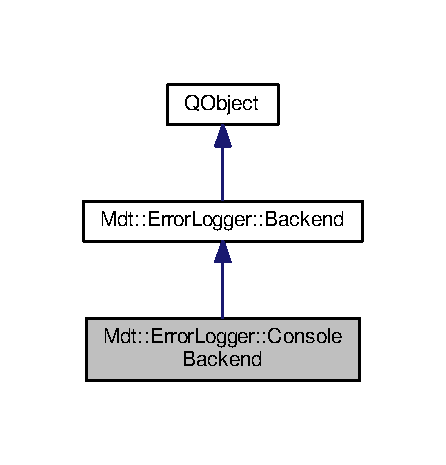
\includegraphics[width=214pt]{class_mdt_1_1_error_logger_1_1_console_backend__inherit__graph}
\end{center}
\end{figure}


Collaboration diagram for Mdt\+:\+:Error\+Logger\+:\+:Console\+Backend\+:
\nopagebreak
\begin{figure}[H]
\begin{center}
\leavevmode
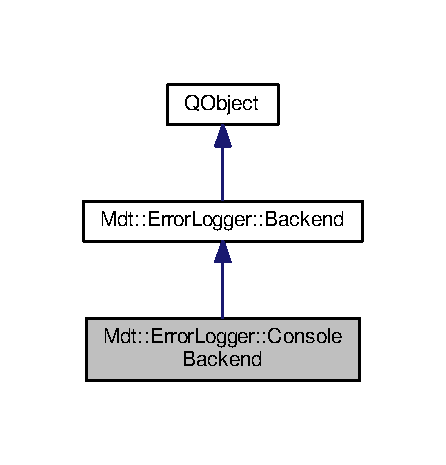
\includegraphics[width=214pt]{class_mdt_1_1_error_logger_1_1_console_backend__coll__graph}
\end{center}
\end{figure}
\subsection*{Public Member Functions}
\begin{DoxyCompactItemize}
\item 
\hyperlink{class_mdt_1_1_error_logger_1_1_console_backend_a79446af5d7658fba5075131f2a0b10dd}{Console\+Backend} (Q\+Object $\ast$parent=nullptr)
\begin{DoxyCompactList}\small\item\em Constructor. \end{DoxyCompactList}\item 
\hyperlink{class_mdt_1_1_error_logger_1_1_console_backend_a7ac5878daa1e4204884d62c592de0e57}{$\sim$\+Console\+Backend} ()
\begin{DoxyCompactList}\small\item\em Destructor. \end{DoxyCompactList}\item 
void \hyperlink{class_mdt_1_1_error_logger_1_1_console_backend_a2d30700dd6a91c244d68bd3670fdbc33}{log\+Error} (const \hyperlink{class_mdt_1_1_error}{Error} \&error)
\begin{DoxyCompactList}\small\item\em Log given error. \end{DoxyCompactList}\end{DoxyCompactItemize}
\subsection*{Additional Inherited Members}


\subsection{Detailed Description}
Console backend for error \hyperlink{class_mdt_1_1_error_logger_1_1_logger}{Logger}. 

Definition at line 31 of file Console\+Backend.\+h.



\subsection{Constructor \& Destructor Documentation}
\index{Mdt\+::\+Error\+Logger\+::\+Console\+Backend@{Mdt\+::\+Error\+Logger\+::\+Console\+Backend}!Console\+Backend@{Console\+Backend}}
\index{Console\+Backend@{Console\+Backend}!Mdt\+::\+Error\+Logger\+::\+Console\+Backend@{Mdt\+::\+Error\+Logger\+::\+Console\+Backend}}
\subsubsection[{\texorpdfstring{Console\+Backend(\+Q\+Object $\ast$parent=nullptr)}{ConsoleBackend(QObject *parent=nullptr)}}]{\setlength{\rightskip}{0pt plus 5cm}Mdt\+::\+Error\+Logger\+::\+Console\+Backend\+::\+Console\+Backend (
\begin{DoxyParamCaption}
\item[{Q\+Object $\ast$}]{parent = {\ttfamily nullptr}}
\end{DoxyParamCaption}
)}\hypertarget{class_mdt_1_1_error_logger_1_1_console_backend_a79446af5d7658fba5075131f2a0b10dd}{}\label{class_mdt_1_1_error_logger_1_1_console_backend_a79446af5d7658fba5075131f2a0b10dd}


Constructor. 



Definition at line 30 of file Console\+Backend.\+cpp.

\index{Mdt\+::\+Error\+Logger\+::\+Console\+Backend@{Mdt\+::\+Error\+Logger\+::\+Console\+Backend}!````~Console\+Backend@{$\sim$\+Console\+Backend}}
\index{````~Console\+Backend@{$\sim$\+Console\+Backend}!Mdt\+::\+Error\+Logger\+::\+Console\+Backend@{Mdt\+::\+Error\+Logger\+::\+Console\+Backend}}
\subsubsection[{\texorpdfstring{$\sim$\+Console\+Backend()}{~ConsoleBackend()}}]{\setlength{\rightskip}{0pt plus 5cm}Mdt\+::\+Error\+Logger\+::\+Console\+Backend\+::$\sim$\+Console\+Backend (
\begin{DoxyParamCaption}
{}
\end{DoxyParamCaption}
)}\hypertarget{class_mdt_1_1_error_logger_1_1_console_backend_a7ac5878daa1e4204884d62c592de0e57}{}\label{class_mdt_1_1_error_logger_1_1_console_backend_a7ac5878daa1e4204884d62c592de0e57}


Destructor. 



Definition at line 35 of file Console\+Backend.\+cpp.



\subsection{Member Function Documentation}
\index{Mdt\+::\+Error\+Logger\+::\+Console\+Backend@{Mdt\+::\+Error\+Logger\+::\+Console\+Backend}!log\+Error@{log\+Error}}
\index{log\+Error@{log\+Error}!Mdt\+::\+Error\+Logger\+::\+Console\+Backend@{Mdt\+::\+Error\+Logger\+::\+Console\+Backend}}
\subsubsection[{\texorpdfstring{log\+Error(const Error \&error)}{logError(const Error &error)}}]{\setlength{\rightskip}{0pt plus 5cm}void Mdt\+::\+Error\+Logger\+::\+Console\+Backend\+::log\+Error (
\begin{DoxyParamCaption}
\item[{const {\bf Error} \&}]{error}
\end{DoxyParamCaption}
)\hspace{0.3cm}{\ttfamily [virtual]}}\hypertarget{class_mdt_1_1_error_logger_1_1_console_backend_a2d30700dd6a91c244d68bd3670fdbc33}{}\label{class_mdt_1_1_error_logger_1_1_console_backend_a2d30700dd6a91c244d68bd3670fdbc33}


Log given error. 



Implements \hyperlink{class_mdt_1_1_error_logger_1_1_backend_acf37cfc576269934ca8ce04e3601058d}{Mdt\+::\+Error\+Logger\+::\+Backend}.



Definition at line 39 of file Console\+Backend.\+cpp.



The documentation for this class was generated from the following files\+:\begin{DoxyCompactItemize}
\item 
libs/\+Error\+\_\+\+Core/src/\+Mdt/\+Error\+Logger/Console\+Backend.\+h\item 
libs/\+Error\+\_\+\+Core/src/\+Mdt/\+Error\+Logger/Console\+Backend.\+cpp\end{DoxyCompactItemize}

\hypertarget{class_mdt_1_1_deploy_utils_1_1_console_stream}{}\section{Mdt\+:\+:Deploy\+Utils\+:\+:Console\+Stream Class Reference}
\label{class_mdt_1_1_deploy_utils_1_1_console_stream}\index{Mdt\+::\+Deploy\+Utils\+::\+Console\+Stream@{Mdt\+::\+Deploy\+Utils\+::\+Console\+Stream}}


Used to implement \hyperlink{class_mdt_1_1_deploy_utils_1_1_console}{Console}.  




{\ttfamily \#include $<$Console\+Stream.\+h$>$}

\subsection*{Public Member Functions}
\begin{DoxyCompactItemize}
\item 
\hyperlink{class_mdt_1_1_deploy_utils_1_1_console_stream_aa2df420c51b0524d143b4e877293f248}{Console\+Stream} (Qt\+Msg\+Type msg\+Type, int min\+Level, int level)\hypertarget{class_mdt_1_1_deploy_utils_1_1_console_stream_aa2df420c51b0524d143b4e877293f248}{}\label{class_mdt_1_1_deploy_utils_1_1_console_stream_aa2df420c51b0524d143b4e877293f248}

\begin{DoxyCompactList}\small\item\em Construct a stream. \end{DoxyCompactList}\item 
\hyperlink{class_mdt_1_1_deploy_utils_1_1_console_stream}{Console\+Stream} \& \hyperlink{class_mdt_1_1_deploy_utils_1_1_console_stream_ab45818f441936c4e3ede6164850a2c86}{operator$<$$<$} (int v)\hypertarget{class_mdt_1_1_deploy_utils_1_1_console_stream_ab45818f441936c4e3ede6164850a2c86}{}\label{class_mdt_1_1_deploy_utils_1_1_console_stream_ab45818f441936c4e3ede6164850a2c86}

\begin{DoxyCompactList}\small\item\em Writes {\itshape v} to the stream and returns a reference to the stream. \end{DoxyCompactList}\item 
\hyperlink{class_mdt_1_1_deploy_utils_1_1_console_stream}{Console\+Stream} \& \hyperlink{class_mdt_1_1_deploy_utils_1_1_console_stream_a9fd2ecfe4311b0cdd3b9536f24314af7}{operator$<$$<$} (const char $\ast$str)\hypertarget{class_mdt_1_1_deploy_utils_1_1_console_stream_a9fd2ecfe4311b0cdd3b9536f24314af7}{}\label{class_mdt_1_1_deploy_utils_1_1_console_stream_a9fd2ecfe4311b0cdd3b9536f24314af7}

\begin{DoxyCompactList}\small\item\em Writes {\itshape str} to the stream and returns a reference to the stream. \end{DoxyCompactList}\item 
\hyperlink{class_mdt_1_1_deploy_utils_1_1_console_stream}{Console\+Stream} \& \hyperlink{class_mdt_1_1_deploy_utils_1_1_console_stream_aebf5221a69df6dfb11c0a0c666e00653}{operator$<$$<$} (const Q\+String \&str)\hypertarget{class_mdt_1_1_deploy_utils_1_1_console_stream_aebf5221a69df6dfb11c0a0c666e00653}{}\label{class_mdt_1_1_deploy_utils_1_1_console_stream_aebf5221a69df6dfb11c0a0c666e00653}

\begin{DoxyCompactList}\small\item\em Writes {\itshape str} to the stream and returns a reference to the stream. \end{DoxyCompactList}\item 
\hyperlink{class_mdt_1_1_deploy_utils_1_1_console_stream}{Console\+Stream} \& \hyperlink{class_mdt_1_1_deploy_utils_1_1_console_stream_ae8b85dd69639169c3e60002a42f38236}{operator$<$$<$} (const \hyperlink{class_mdt_1_1_error}{Mdt\+::\+Error} \&error)\hypertarget{class_mdt_1_1_deploy_utils_1_1_console_stream_ae8b85dd69639169c3e60002a42f38236}{}\label{class_mdt_1_1_deploy_utils_1_1_console_stream_ae8b85dd69639169c3e60002a42f38236}

\begin{DoxyCompactList}\small\item\em Writes {\itshape error} to the stream and returns a reference to the stream. \end{DoxyCompactList}\end{DoxyCompactItemize}


\subsection{Detailed Description}
Used to implement \hyperlink{class_mdt_1_1_deploy_utils_1_1_console}{Console}. 

This class uses Q\+Debug internally, but was designed to expose it in the public headers. This permits to use Q\+Debug for debuging, and, when finished, remove the Q\+Debug include, which permits the compiler to throw a error if we forgot a q\+Debug() somewhere. 

Definition at line 47 of file Console\+Stream.\+h.



The documentation for this class was generated from the following files\+:\begin{DoxyCompactItemize}
\item 
libs/\+Deploy\+Utils\+\_\+\+Core/src/\+Mdt/\+Deploy\+Utils/Console\+Stream.\+h\item 
libs/\+Deploy\+Utils\+\_\+\+Core/src/\+Mdt/\+Deploy\+Utils/Console\+Stream.\+cpp\end{DoxyCompactItemize}

\hypertarget{class_mdt_1_1_core_application}{}\section{Mdt\+:\+:Core\+Application Class Reference}
\label{class_mdt_1_1_core_application}\index{Mdt\+::\+Core\+Application@{Mdt\+::\+Core\+Application}}


\hyperlink{class_mdt_1_1_core_application}{Core\+Application} adds some helper to \hyperlink{class_q_core_application}{Q\+Core\+Application} for application initialization.  




{\ttfamily \#include $<$Core\+Application.\+h$>$}



Inheritance diagram for Mdt\+:\+:Core\+Application\+:
\nopagebreak
\begin{figure}[H]
\begin{center}
\leavevmode
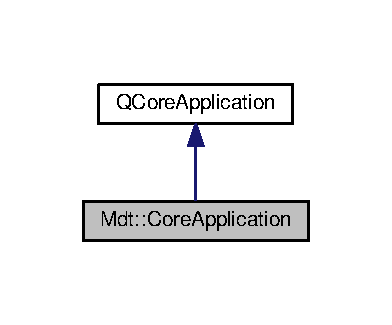
\includegraphics[width=188pt]{class_mdt_1_1_core_application__inherit__graph}
\end{center}
\end{figure}


Collaboration diagram for Mdt\+:\+:Core\+Application\+:
\nopagebreak
\begin{figure}[H]
\begin{center}
\leavevmode
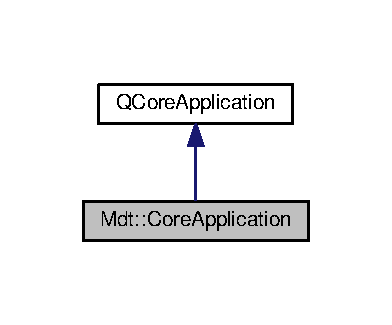
\includegraphics[width=188pt]{class_mdt_1_1_core_application__coll__graph}
\end{center}
\end{figure}
\subsection*{Public Member Functions}
\begin{DoxyCompactItemize}
\item 
\hyperlink{class_mdt_1_1_core_application_a1f9e0cee5d94ec783ea49ec57030bce9}{Core\+Application} (int \&argc, char $\ast$$\ast$argv)
\begin{DoxyCompactList}\small\item\em Construct a core application. \end{DoxyCompactList}\item 
\hyperlink{class_mdt_1_1_core_application_ac91f0fe77618f10cbdf1f5594c2a82ea}{$\sim$\+Core\+Application} ()
\begin{DoxyCompactList}\small\item\em Destroy the core application object. \end{DoxyCompactList}\item 
{\bfseries Core\+Application} (const \hyperlink{class_mdt_1_1_core_application}{Core\+Application} \&)=delete\hypertarget{class_mdt_1_1_core_application_a62325e06671365f59e2e665d154c7980}{}\label{class_mdt_1_1_core_application_a62325e06671365f59e2e665d154c7980}

\item 
\hyperlink{class_mdt_1_1_core_application}{Core\+Application} \& {\bfseries operator=} (const \hyperlink{class_mdt_1_1_core_application}{Core\+Application} \&)=delete\hypertarget{class_mdt_1_1_core_application_a7d289e822b3b564ec1be514f1abe8634}{}\label{class_mdt_1_1_core_application_a7d289e822b3b564ec1be514f1abe8634}

\item 
{\bfseries Core\+Application} (\hyperlink{class_mdt_1_1_core_application}{Core\+Application} \&\&)=delete\hypertarget{class_mdt_1_1_core_application_add05d6ef32f7eaf59573a1d5a1a3e488}{}\label{class_mdt_1_1_core_application_add05d6ef32f7eaf59573a1d5a1a3e488}

\item 
\hyperlink{class_mdt_1_1_core_application}{Core\+Application} \& {\bfseries operator=} (\hyperlink{class_mdt_1_1_core_application}{Core\+Application} \&\&)=delete\hypertarget{class_mdt_1_1_core_application_aceac66ce619e99eba6fbf1039da9a009}{}\label{class_mdt_1_1_core_application_aceac66ce619e99eba6fbf1039da9a009}

\item 
void \hyperlink{class_mdt_1_1_core_application_aa76faa75f09c7ba30406bfd6b2284bd7}{enable\+File\+Logging} ()
\begin{DoxyCompactList}\small\item\em Enable file logging. \end{DoxyCompactList}\item 
Q\+String \hyperlink{class_mdt_1_1_core_application_a48a2915a7876c259347290f1f501df46}{log\+File\+Path} ()
\begin{DoxyCompactList}\small\item\em Get the path to the log file. \end{DoxyCompactList}\item 
void \hyperlink{class_mdt_1_1_core_application_a500820026134788b2c77c880663339d9}{debug\+Environment} ()
\begin{DoxyCompactList}\small\item\em Debug environment. \end{DoxyCompactList}\end{DoxyCompactItemize}
\subsection*{Static Public Member Functions}
\begin{DoxyCompactItemize}
\item 
static Q\+String \hyperlink{class_mdt_1_1_core_application_aa5bf79da0eda7f8dedd2b78bf8025449}{cache\+Directory\+Path} ()
\begin{DoxyCompactList}\small\item\em Get path to the cache directory. \end{DoxyCompactList}\item 
static Q\+String \hyperlink{class_mdt_1_1_core_application_a0509073283a3a23e4ee3cf248739e15c}{qt\+Version} ()
\begin{DoxyCompactList}\small\item\em Get Qt library version. \end{DoxyCompactList}\item 
static Q\+String \hyperlink{class_mdt_1_1_core_application_a43d5e4e3b163250cba37c0071fb9f7ea}{mdt\+Version} ()
\begin{DoxyCompactList}\small\item\em Get \hyperlink{namespace_mdt}{Mdt} library version. \end{DoxyCompactList}\end{DoxyCompactItemize}


\subsection{Detailed Description}
\hyperlink{class_mdt_1_1_core_application}{Core\+Application} adds some helper to \hyperlink{class_q_core_application}{Q\+Core\+Application} for application initialization. 

\begin{DoxySeeAlso}{See also}
\hyperlink{class_q_core_application}{Q\+Core\+Application} 
\end{DoxySeeAlso}


Definition at line 36 of file Core\+Application.\+h.



\subsection{Constructor \& Destructor Documentation}
\index{Mdt\+::\+Core\+Application@{Mdt\+::\+Core\+Application}!Core\+Application@{Core\+Application}}
\index{Core\+Application@{Core\+Application}!Mdt\+::\+Core\+Application@{Mdt\+::\+Core\+Application}}
\subsubsection[{\texorpdfstring{Core\+Application(int \&argc, char $\ast$$\ast$argv)}{CoreApplication(int &argc, char **argv)}}]{\setlength{\rightskip}{0pt plus 5cm}Mdt\+::\+Core\+Application\+::\+Core\+Application (
\begin{DoxyParamCaption}
\item[{int \&}]{argc, }
\item[{char $\ast$$\ast$}]{argv}
\end{DoxyParamCaption}
)}\hypertarget{class_mdt_1_1_core_application_a1f9e0cee5d94ec783ea49ec57030bce9}{}\label{class_mdt_1_1_core_application_a1f9e0cee5d94ec783ea49ec57030bce9}


Construct a core application. 



Definition at line 26 of file Core\+Application.\+cpp.

\index{Mdt\+::\+Core\+Application@{Mdt\+::\+Core\+Application}!````~Core\+Application@{$\sim$\+Core\+Application}}
\index{````~Core\+Application@{$\sim$\+Core\+Application}!Mdt\+::\+Core\+Application@{Mdt\+::\+Core\+Application}}
\subsubsection[{\texorpdfstring{$\sim$\+Core\+Application()}{~CoreApplication()}}]{\setlength{\rightskip}{0pt plus 5cm}Mdt\+::\+Core\+Application\+::$\sim$\+Core\+Application (
\begin{DoxyParamCaption}
{}
\end{DoxyParamCaption}
)}\hypertarget{class_mdt_1_1_core_application_ac91f0fe77618f10cbdf1f5594c2a82ea}{}\label{class_mdt_1_1_core_application_ac91f0fe77618f10cbdf1f5594c2a82ea}


Destroy the core application object. 



Definition at line 32 of file Core\+Application.\+cpp.



\subsection{Member Function Documentation}
\index{Mdt\+::\+Core\+Application@{Mdt\+::\+Core\+Application}!cache\+Directory\+Path@{cache\+Directory\+Path}}
\index{cache\+Directory\+Path@{cache\+Directory\+Path}!Mdt\+::\+Core\+Application@{Mdt\+::\+Core\+Application}}
\subsubsection[{\texorpdfstring{cache\+Directory\+Path()}{cacheDirectoryPath()}}]{\setlength{\rightskip}{0pt plus 5cm}Q\+String Mdt\+::\+Core\+Application\+::cache\+Directory\+Path (
\begin{DoxyParamCaption}
{}
\end{DoxyParamCaption}
)\hspace{0.3cm}{\ttfamily [static]}}\hypertarget{class_mdt_1_1_core_application_aa5bf79da0eda7f8dedd2b78bf8025449}{}\label{class_mdt_1_1_core_application_aa5bf79da0eda7f8dedd2b78bf8025449}


Get path to the cache directory. 

Returns \hyperlink{class_mdt_1_1_standard_paths_a2ca803e5a6b9fb2a4808968becfb86de}{Standard\+Paths\+::cache\+Directory\+Path()} 

Definition at line 46 of file Core\+Application.\+cpp.



References Mdt\+::\+Core\+Application\+Impl\+::cache\+Directory\+Path().

\index{Mdt\+::\+Core\+Application@{Mdt\+::\+Core\+Application}!debug\+Environment@{debug\+Environment}}
\index{debug\+Environment@{debug\+Environment}!Mdt\+::\+Core\+Application@{Mdt\+::\+Core\+Application}}
\subsubsection[{\texorpdfstring{debug\+Environment()}{debugEnvironment()}}]{\setlength{\rightskip}{0pt plus 5cm}void Mdt\+::\+Core\+Application\+::debug\+Environment (
\begin{DoxyParamCaption}
{}
\end{DoxyParamCaption}
)}\hypertarget{class_mdt_1_1_core_application_a500820026134788b2c77c880663339d9}{}\label{class_mdt_1_1_core_application_a500820026134788b2c77c880663339d9}


Debug environment. 

Will print various informations, like libraries versions, paths to some directories, etc.. to the console. 

Definition at line 61 of file Core\+Application.\+cpp.

\index{Mdt\+::\+Core\+Application@{Mdt\+::\+Core\+Application}!enable\+File\+Logging@{enable\+File\+Logging}}
\index{enable\+File\+Logging@{enable\+File\+Logging}!Mdt\+::\+Core\+Application@{Mdt\+::\+Core\+Application}}
\subsubsection[{\texorpdfstring{enable\+File\+Logging()}{enableFileLogging()}}]{\setlength{\rightskip}{0pt plus 5cm}void Mdt\+::\+Core\+Application\+::enable\+File\+Logging (
\begin{DoxyParamCaption}
{}
\end{DoxyParamCaption}
)}\hypertarget{class_mdt_1_1_core_application_aa76faa75f09c7ba30406bfd6b2284bd7}{}\label{class_mdt_1_1_core_application_aa76faa75f09c7ba30406bfd6b2284bd7}


Enable file logging. 

After file logging was enabled, errors that are committed using \hyperlink{class_mdt_1_1_error_a1b4a57bd4177d2985abd62b6b49a43f8}{Mdt\+::\+Error\+::commit()} are added to the log file {\itshape \hyperlink{class_mdt_1_1_core_application_a48a2915a7876c259347290f1f501df46}{log\+File\+Path()}} . 

Definition at line 36 of file Core\+Application.\+cpp.



References Mdt\+::\+Core\+Application\+Impl\+::\+Application\+Name\+And\+Pid.

\index{Mdt\+::\+Core\+Application@{Mdt\+::\+Core\+Application}!log\+File\+Path@{log\+File\+Path}}
\index{log\+File\+Path@{log\+File\+Path}!Mdt\+::\+Core\+Application@{Mdt\+::\+Core\+Application}}
\subsubsection[{\texorpdfstring{log\+File\+Path()}{logFilePath()}}]{\setlength{\rightskip}{0pt plus 5cm}Q\+String Mdt\+::\+Core\+Application\+::log\+File\+Path (
\begin{DoxyParamCaption}
{}
\end{DoxyParamCaption}
)}\hypertarget{class_mdt_1_1_core_application_a48a2915a7876c259347290f1f501df46}{}\label{class_mdt_1_1_core_application_a48a2915a7876c259347290f1f501df46}


Get the path to the log file. 



Definition at line 41 of file Core\+Application.\+cpp.

\index{Mdt\+::\+Core\+Application@{Mdt\+::\+Core\+Application}!mdt\+Version@{mdt\+Version}}
\index{mdt\+Version@{mdt\+Version}!Mdt\+::\+Core\+Application@{Mdt\+::\+Core\+Application}}
\subsubsection[{\texorpdfstring{mdt\+Version()}{mdtVersion()}}]{\setlength{\rightskip}{0pt plus 5cm}Q\+String Mdt\+::\+Core\+Application\+::mdt\+Version (
\begin{DoxyParamCaption}
{}
\end{DoxyParamCaption}
)\hspace{0.3cm}{\ttfamily [static]}}\hypertarget{class_mdt_1_1_core_application_a43d5e4e3b163250cba37c0071fb9f7ea}{}\label{class_mdt_1_1_core_application_a43d5e4e3b163250cba37c0071fb9f7ea}


Get \hyperlink{namespace_mdt}{Mdt} library version. 



Definition at line 56 of file Core\+Application.\+cpp.



References Mdt\+::\+Core\+Application\+Impl\+::mdt\+Version().

\index{Mdt\+::\+Core\+Application@{Mdt\+::\+Core\+Application}!qt\+Version@{qt\+Version}}
\index{qt\+Version@{qt\+Version}!Mdt\+::\+Core\+Application@{Mdt\+::\+Core\+Application}}
\subsubsection[{\texorpdfstring{qt\+Version()}{qtVersion()}}]{\setlength{\rightskip}{0pt plus 5cm}Q\+String Mdt\+::\+Core\+Application\+::qt\+Version (
\begin{DoxyParamCaption}
{}
\end{DoxyParamCaption}
)\hspace{0.3cm}{\ttfamily [static]}}\hypertarget{class_mdt_1_1_core_application_a0509073283a3a23e4ee3cf248739e15c}{}\label{class_mdt_1_1_core_application_a0509073283a3a23e4ee3cf248739e15c}


Get Qt library version. 



Definition at line 51 of file Core\+Application.\+cpp.



References Mdt\+::\+Core\+Application\+Impl\+::qt\+Version().



The documentation for this class was generated from the following files\+:\begin{DoxyCompactItemize}
\item 
libs/\+Application\+\_\+\+Core/src/\+Mdt/Core\+Application.\+h\item 
libs/\+Application\+\_\+\+Core/src/\+Mdt/Core\+Application.\+cpp\end{DoxyCompactItemize}

\hypertarget{class_mdt_1_1_core_application_impl}{}\section{Mdt\+:\+:Core\+Application\+Impl Class Reference}
\label{class_mdt_1_1_core_application_impl}\index{Mdt\+::\+Core\+Application\+Impl@{Mdt\+::\+Core\+Application\+Impl}}


Implementation for \hyperlink{class_mdt_1_1_core_application}{Core\+Application} and derived classes.  




{\ttfamily \#include $<$Core\+Application\+Impl.\+h$>$}



Inheritance diagram for Mdt\+:\+:Core\+Application\+Impl\+:\nopagebreak
\begin{figure}[H]
\begin{center}
\leavevmode
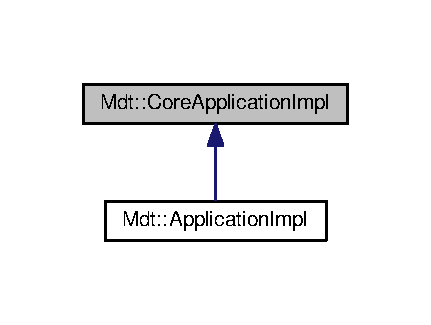
\includegraphics[width=207pt]{class_mdt_1_1_core_application_impl__inherit__graph}
\end{center}
\end{figure}
\subsection*{Public Types}
\subsection*{Public Member Functions}
\begin{DoxyCompactItemize}
\item 
\hyperlink{class_mdt_1_1_core_application_impl_ab97b101b57a2fa8410e39b940e022c4c}{Core\+Application\+Impl} ()\hypertarget{class_mdt_1_1_core_application_impl_ab97b101b57a2fa8410e39b940e022c4c}{}\label{class_mdt_1_1_core_application_impl_ab97b101b57a2fa8410e39b940e022c4c}

\begin{DoxyCompactList}\small\item\em Constructor. \end{DoxyCompactList}\item 
\hyperlink{class_mdt_1_1_core_application_impl_aa17f799e5d756ca8c5a89196fcbd8e90}{$\sim$\+Core\+Application\+Impl} ()\hypertarget{class_mdt_1_1_core_application_impl_aa17f799e5d756ca8c5a89196fcbd8e90}{}\label{class_mdt_1_1_core_application_impl_aa17f799e5d756ca8c5a89196fcbd8e90}

\begin{DoxyCompactList}\small\item\em Destructor. \end{DoxyCompactList}\item 
void \hyperlink{class_mdt_1_1_core_application_impl_a3bd40afeeb08ddcba8cbfc78c177305b}{enable\+File\+Logging} (\hyperlink{class_mdt_1_1_core_application_impl_aa5fed8435e22870a870005ee28ff6221}{Log\+File\+Name\+Format} format)\hypertarget{class_mdt_1_1_core_application_impl_a3bd40afeeb08ddcba8cbfc78c177305b}{}\label{class_mdt_1_1_core_application_impl_a3bd40afeeb08ddcba8cbfc78c177305b}

\begin{DoxyCompactList}\small\item\em Enable file logging. \end{DoxyCompactList}\item 
bool \hyperlink{class_mdt_1_1_core_application_impl_a42a42b5d134b70a6e1c0452f29c73912}{is\+File\+Logging\+Enabled} () const \hypertarget{class_mdt_1_1_core_application_impl_a42a42b5d134b70a6e1c0452f29c73912}{}\label{class_mdt_1_1_core_application_impl_a42a42b5d134b70a6e1c0452f29c73912}

\begin{DoxyCompactList}\small\item\em Check if file logging is enabled. \end{DoxyCompactList}\item 
Q\+String \hyperlink{class_mdt_1_1_core_application_impl_abc2b6b3ab83fdf2fd9dca1447bc82418}{log\+File\+Path} ()\hypertarget{class_mdt_1_1_core_application_impl_abc2b6b3ab83fdf2fd9dca1447bc82418}{}\label{class_mdt_1_1_core_application_impl_abc2b6b3ab83fdf2fd9dca1447bc82418}

\begin{DoxyCompactList}\small\item\em Get the path to the log file. \end{DoxyCompactList}\item 
void \hyperlink{class_mdt_1_1_core_application_impl_a29a336750c7ea04a570fbd769497c98f}{debug\+Environment} (const Q\+String\+List \&entries)\hypertarget{class_mdt_1_1_core_application_impl_a29a336750c7ea04a570fbd769497c98f}{}\label{class_mdt_1_1_core_application_impl_a29a336750c7ea04a570fbd769497c98f}

\begin{DoxyCompactList}\small\item\em Debug environment. \end{DoxyCompactList}\item 
Q\+String\+List \hyperlink{class_mdt_1_1_core_application_impl_abbafc463e7c820e42f967813e9e7ae7a}{common\+Environment\+Entries} ()\hypertarget{class_mdt_1_1_core_application_impl_abbafc463e7c820e42f967813e9e7ae7a}{}\label{class_mdt_1_1_core_application_impl_abbafc463e7c820e42f967813e9e7ae7a}

\begin{DoxyCompactList}\small\item\em Get common environment entries. \end{DoxyCompactList}\end{DoxyCompactItemize}
\subsection*{Static Public Member Functions}
\begin{DoxyCompactItemize}
\item 
static Q\+String \hyperlink{class_mdt_1_1_core_application_impl_a5335fddfbe75c3944199d30d201ece04}{log\+Directory\+Path} ()
\begin{DoxyCompactList}\small\item\em Get the path to log file directory. \end{DoxyCompactList}\item 
static Q\+String \hyperlink{class_mdt_1_1_core_application_impl_a4d78244d773ca265a7108275f2295ca2}{cache\+Directory\+Path} ()
\begin{DoxyCompactList}\small\item\em Get path to the cache directory. \end{DoxyCompactList}\item 
static Q\+String \hyperlink{class_mdt_1_1_core_application_impl_a7c1f7ed8684b4d3ec8aa68a0da5d2d04}{qt\+Version} ()\hypertarget{class_mdt_1_1_core_application_impl_a7c1f7ed8684b4d3ec8aa68a0da5d2d04}{}\label{class_mdt_1_1_core_application_impl_a7c1f7ed8684b4d3ec8aa68a0da5d2d04}

\begin{DoxyCompactList}\small\item\em Get Qt library version. \end{DoxyCompactList}\item 
static Q\+String \hyperlink{class_mdt_1_1_core_application_impl_af8728d7751e6041d5680d99f033ae52d}{mdt\+Version} ()\hypertarget{class_mdt_1_1_core_application_impl_af8728d7751e6041d5680d99f033ae52d}{}\label{class_mdt_1_1_core_application_impl_af8728d7751e6041d5680d99f033ae52d}

\begin{DoxyCompactList}\small\item\em Get \hyperlink{namespace_mdt}{Mdt} library version. \end{DoxyCompactList}\end{DoxyCompactItemize}


\subsection{Detailed Description}
Implementation for \hyperlink{class_mdt_1_1_core_application}{Core\+Application} and derived classes. 

Definition at line 34 of file Core\+Application\+Impl.\+h.



\subsection{Member Enumeration Documentation}
\index{Mdt\+::\+Core\+Application\+Impl@{Mdt\+::\+Core\+Application\+Impl}!Log\+File\+Name\+Format@{Log\+File\+Name\+Format}}
\index{Log\+File\+Name\+Format@{Log\+File\+Name\+Format}!Mdt\+::\+Core\+Application\+Impl@{Mdt\+::\+Core\+Application\+Impl}}
\subsubsection[{\texorpdfstring{Log\+File\+Name\+Format}{LogFileNameFormat}}]{\setlength{\rightskip}{0pt plus 5cm}enum {\bf Mdt\+::\+Core\+Application\+Impl\+::\+Log\+File\+Name\+Format}}\hypertarget{class_mdt_1_1_core_application_impl_aa5fed8435e22870a870005ee28ff6221}{}\label{class_mdt_1_1_core_application_impl_aa5fed8435e22870a870005ee28ff6221}


Log file name format. 

\begin{Desc}
\item[Enumerator]\par
\begin{description}
\index{Application\+Name@{Application\+Name}!Mdt\+::\+Core\+Application\+Impl@{Mdt\+::\+Core\+Application\+Impl}}\index{Mdt\+::\+Core\+Application\+Impl@{Mdt\+::\+Core\+Application\+Impl}!Application\+Name@{Application\+Name}}\item[{\em 
Application\+Name\hypertarget{class_mdt_1_1_core_application_impl_aa5fed8435e22870a870005ee28ff6221ab47da4311e174cd5978c765033f0060e}{}\label{class_mdt_1_1_core_application_impl_aa5fed8435e22870a870005ee28ff6221ab47da4311e174cd5978c765033f0060e}
}]Log file name will be application\+Name.\+log \index{Application\+Name\+And\+Pid@{Application\+Name\+And\+Pid}!Mdt\+::\+Core\+Application\+Impl@{Mdt\+::\+Core\+Application\+Impl}}\index{Mdt\+::\+Core\+Application\+Impl@{Mdt\+::\+Core\+Application\+Impl}!Application\+Name\+And\+Pid@{Application\+Name\+And\+Pid}}\item[{\em 
Application\+Name\+And\+Pid\hypertarget{class_mdt_1_1_core_application_impl_aa5fed8435e22870a870005ee28ff6221ae817e774fbf9d95b9b720ce7da8e6604}{}\label{class_mdt_1_1_core_application_impl_aa5fed8435e22870a870005ee28ff6221ae817e774fbf9d95b9b720ce7da8e6604}
}]Log file name will be application\+Name\+\_\+pid.\+log \end{description}
\end{Desc}


Definition at line 42 of file Core\+Application\+Impl.\+h.



\subsection{Member Function Documentation}
\index{Mdt\+::\+Core\+Application\+Impl@{Mdt\+::\+Core\+Application\+Impl}!cache\+Directory\+Path@{cache\+Directory\+Path}}
\index{cache\+Directory\+Path@{cache\+Directory\+Path}!Mdt\+::\+Core\+Application\+Impl@{Mdt\+::\+Core\+Application\+Impl}}
\subsubsection[{\texorpdfstring{cache\+Directory\+Path()}{cacheDirectoryPath()}}]{\setlength{\rightskip}{0pt plus 5cm}static Q\+String Mdt\+::\+Core\+Application\+Impl\+::cache\+Directory\+Path (
\begin{DoxyParamCaption}
{}
\end{DoxyParamCaption}
)\hspace{0.3cm}{\ttfamily [inline]}, {\ttfamily [static]}}\hypertarget{class_mdt_1_1_core_application_impl_a4d78244d773ca265a7108275f2295ca2}{}\label{class_mdt_1_1_core_application_impl_a4d78244d773ca265a7108275f2295ca2}


Get path to the cache directory. 

Returns \hyperlink{class_mdt_1_1_standard_paths_a2ca803e5a6b9fb2a4808968becfb86de}{Standard\+Paths\+::cache\+Directory\+Path()} 

Definition at line 94 of file Core\+Application\+Impl.\+h.

\index{Mdt\+::\+Core\+Application\+Impl@{Mdt\+::\+Core\+Application\+Impl}!log\+Directory\+Path@{log\+Directory\+Path}}
\index{log\+Directory\+Path@{log\+Directory\+Path}!Mdt\+::\+Core\+Application\+Impl@{Mdt\+::\+Core\+Application\+Impl}}
\subsubsection[{\texorpdfstring{log\+Directory\+Path()}{logDirectoryPath()}}]{\setlength{\rightskip}{0pt plus 5cm}static Q\+String Mdt\+::\+Core\+Application\+Impl\+::log\+Directory\+Path (
\begin{DoxyParamCaption}
{}
\end{DoxyParamCaption}
)\hspace{0.3cm}{\ttfamily [inline]}, {\ttfamily [static]}}\hypertarget{class_mdt_1_1_core_application_impl_a5335fddfbe75c3944199d30d201ece04}{}\label{class_mdt_1_1_core_application_impl_a5335fddfbe75c3944199d30d201ece04}


Get the path to log file directory. 

Returns \hyperlink{class_mdt_1_1_standard_paths_aa45caeb4d2b4a5c539d301d800a7deac}{Standard\+Paths\+::log\+Directory\+Path()} 

Definition at line 78 of file Core\+Application\+Impl.\+h.



The documentation for this class was generated from the following files\+:\begin{DoxyCompactItemize}
\item 
libs/\+Application\+\_\+\+Core/src/\+Mdt/Core\+Application\+Impl.\+h\item 
libs/\+Application\+\_\+\+Core/src/\+Mdt/Core\+Application\+Impl.\+cpp\end{DoxyCompactItemize}

\hypertarget{class_mdt_1_1_plain_text_1_1_csv_common_settings}{}\section{Mdt\+:\+:Plain\+Text\+:\+:Csv\+Common\+Settings Class Reference}
\label{class_mdt_1_1_plain_text_1_1_csv_common_settings}\index{Mdt\+::\+Plain\+Text\+::\+Csv\+Common\+Settings@{Mdt\+::\+Plain\+Text\+::\+Csv\+Common\+Settings}}


Common C\+SV settings.  




{\ttfamily \#include $<$Csv\+Common\+Settings.\+h$>$}



Inheritance diagram for Mdt\+:\+:Plain\+Text\+:\+:Csv\+Common\+Settings\+:\nopagebreak
\begin{figure}[H]
\begin{center}
\leavevmode
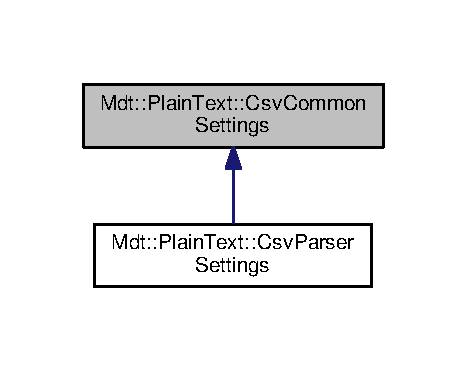
\includegraphics[width=224pt]{class_mdt_1_1_plain_text_1_1_csv_common_settings__inherit__graph}
\end{center}
\end{figure}


\subsection{Detailed Description}
Common C\+SV settings. 

\begin{DoxyNote}{Note}
Some part of this A\+PI documentation refers to C\+S\+V-\/1203 standard. C\+S\+V-\/1203 is a open standard available here\+: \href{http://mastpoint.com/csv-1203}{\tt http\+://mastpoint.\+com/csv-\/1203} 
\end{DoxyNote}


Definition at line 35 of file Csv\+Common\+Settings.\+h.



The documentation for this class was generated from the following file\+:\begin{DoxyCompactItemize}
\item 
libs/\+Plain\+Text\+\_\+\+Core/src/\+Mdt/\+Plain\+Text/Csv\+Common\+Settings.\+h\end{DoxyCompactItemize}

\hypertarget{class_mdt_1_1_plain_text_1_1_csv_file_parser}{}\section{Mdt\+:\+:Plain\+Text\+:\+:Csv\+File\+Parser Class Reference}
\label{class_mdt_1_1_plain_text_1_1_csv_file_parser}\index{Mdt\+::\+Plain\+Text\+::\+Csv\+File\+Parser@{Mdt\+::\+Plain\+Text\+::\+Csv\+File\+Parser}}


C\+SV parser that acts on a file as input.  




{\ttfamily \#include $<$Csv\+File\+Parser.\+h$>$}

\subsection*{Public Member Functions}
\begin{DoxyCompactItemize}
\item 
\hyperlink{class_mdt_1_1_plain_text_1_1_csv_file_parser_ac7913634006a58b5a5c2b53a3de21a57}{Csv\+File\+Parser} ()
\begin{DoxyCompactList}\small\item\em Default constructor. \end{DoxyCompactList}\item 
void \hyperlink{class_mdt_1_1_plain_text_1_1_csv_file_parser_ae5a305689ca8b7aaee94f51b95464135}{set\+Csv\+Settings} (const \hyperlink{class_mdt_1_1_plain_text_1_1_csv_parser_settings}{Csv\+Parser\+Settings} \&settings)
\begin{DoxyCompactList}\small\item\em Set C\+SV settings. \end{DoxyCompactList}\item 
bool \hyperlink{class_mdt_1_1_plain_text_1_1_csv_file_parser_a9b81b6061eb86888af9fe51752f8617a}{open\+File} (const Q\+File\+Info \&file\+Info, const Q\+Byte\+Array \&encoding)
\begin{DoxyCompactList}\small\item\em Open C\+SV file. \end{DoxyCompactList}\item 
bool \hyperlink{class_mdt_1_1_plain_text_1_1_csv_file_parser_a2e8e57b7cd46bccf4c6953b9654c73fa}{is\+Open} () const 
\begin{DoxyCompactList}\small\item\em Check if a C\+SV file is open. \end{DoxyCompactList}\item 
void \hyperlink{class_mdt_1_1_plain_text_1_1_csv_file_parser_aee81b90521927b6f8eb1482633c0a67d}{close\+File} ()
\begin{DoxyCompactList}\small\item\em Close C\+SV file. \end{DoxyCompactList}\item 
bool \hyperlink{class_mdt_1_1_plain_text_1_1_csv_file_parser_af71b58865205fac3eebd00b416f58a2f}{at\+End} () const 
\begin{DoxyCompactList}\small\item\em Check about end of file. \end{DoxyCompactList}\item 
\hyperlink{class_mdt_1_1_expected}{Mdt\+::\+Expected}$<$ String\+Record $>$ \hyperlink{class_mdt_1_1_plain_text_1_1_csv_file_parser_ab0b04108ed3e2ea4fa272567d7bed2ed}{read\+Line} ()
\begin{DoxyCompactList}\small\item\em Read one line in C\+SV file. \end{DoxyCompactList}\item 
\hyperlink{class_mdt_1_1_expected}{Mdt\+::\+Expected}$<$ String\+Record\+List $>$ \hyperlink{class_mdt_1_1_plain_text_1_1_csv_file_parser_a205ee7b5fb424e48652ffeb722f2f9cb}{read\+All} ()
\begin{DoxyCompactList}\small\item\em Read the entire C\+SV file. \end{DoxyCompactList}\item 
\hyperlink{class_mdt_1_1_error}{Mdt\+::\+Error} \hyperlink{class_mdt_1_1_plain_text_1_1_csv_file_parser_a7c9d6b5675ee9d5b84d99197264ebffb}{last\+Error} () const 
\begin{DoxyCompactList}\small\item\em Get last error. \end{DoxyCompactList}\end{DoxyCompactItemize}


\subsection{Detailed Description}
C\+SV parser that acts on a file as input. 

\begin{DoxyNote}{Note}
Some part of this A\+PI documentation refers to following standards\+: \begin{DoxyItemize}
\item C\+S\+V-\/1203 available here\+: \href{http://mastpoint.com/csv-1203}{\tt http\+://mastpoint.\+com/csv-\/1203} \item R\+FC 4180 available here\+: \href{https://tools.ietf.org/html/rfc4180}{\tt https\+://tools.\+ietf.\+org/html/rfc4180} \end{DoxyItemize}

\end{DoxyNote}


Definition at line 48 of file Csv\+File\+Parser.\+h.



\subsection{Constructor \& Destructor Documentation}
\index{Mdt\+::\+Plain\+Text\+::\+Csv\+File\+Parser@{Mdt\+::\+Plain\+Text\+::\+Csv\+File\+Parser}!Csv\+File\+Parser@{Csv\+File\+Parser}}
\index{Csv\+File\+Parser@{Csv\+File\+Parser}!Mdt\+::\+Plain\+Text\+::\+Csv\+File\+Parser@{Mdt\+::\+Plain\+Text\+::\+Csv\+File\+Parser}}
\subsubsection[{\texorpdfstring{Csv\+File\+Parser()}{CsvFileParser()}}]{\setlength{\rightskip}{0pt plus 5cm}Mdt\+::\+Plain\+Text\+::\+Csv\+File\+Parser\+::\+Csv\+File\+Parser (
\begin{DoxyParamCaption}
{}
\end{DoxyParamCaption}
)}\hypertarget{class_mdt_1_1_plain_text_1_1_csv_file_parser_ac7913634006a58b5a5c2b53a3de21a57}{}\label{class_mdt_1_1_plain_text_1_1_csv_file_parser_ac7913634006a58b5a5c2b53a3de21a57}


Default constructor. 



Definition at line 30 of file Csv\+File\+Parser.\+cpp.



\subsection{Member Function Documentation}
\index{Mdt\+::\+Plain\+Text\+::\+Csv\+File\+Parser@{Mdt\+::\+Plain\+Text\+::\+Csv\+File\+Parser}!at\+End@{at\+End}}
\index{at\+End@{at\+End}!Mdt\+::\+Plain\+Text\+::\+Csv\+File\+Parser@{Mdt\+::\+Plain\+Text\+::\+Csv\+File\+Parser}}
\subsubsection[{\texorpdfstring{at\+End() const }{atEnd() const }}]{\setlength{\rightskip}{0pt plus 5cm}bool Mdt\+::\+Plain\+Text\+::\+Csv\+File\+Parser\+::at\+End (
\begin{DoxyParamCaption}
{}
\end{DoxyParamCaption}
) const}\hypertarget{class_mdt_1_1_plain_text_1_1_csv_file_parser_af71b58865205fac3eebd00b416f58a2f}{}\label{class_mdt_1_1_plain_text_1_1_csv_file_parser_af71b58865205fac3eebd00b416f58a2f}


Check about end of file. 

If no file is open, this function returns allways true 

Definition at line 82 of file Csv\+File\+Parser.\+cpp.

\index{Mdt\+::\+Plain\+Text\+::\+Csv\+File\+Parser@{Mdt\+::\+Plain\+Text\+::\+Csv\+File\+Parser}!close\+File@{close\+File}}
\index{close\+File@{close\+File}!Mdt\+::\+Plain\+Text\+::\+Csv\+File\+Parser@{Mdt\+::\+Plain\+Text\+::\+Csv\+File\+Parser}}
\subsubsection[{\texorpdfstring{close\+File()}{closeFile()}}]{\setlength{\rightskip}{0pt plus 5cm}void Mdt\+::\+Plain\+Text\+::\+Csv\+File\+Parser\+::close\+File (
\begin{DoxyParamCaption}
{}
\end{DoxyParamCaption}
)}\hypertarget{class_mdt_1_1_plain_text_1_1_csv_file_parser_aee81b90521927b6f8eb1482633c0a67d}{}\label{class_mdt_1_1_plain_text_1_1_csv_file_parser_aee81b90521927b6f8eb1482633c0a67d}


Close C\+SV file. 



Definition at line 76 of file Csv\+File\+Parser.\+cpp.

\index{Mdt\+::\+Plain\+Text\+::\+Csv\+File\+Parser@{Mdt\+::\+Plain\+Text\+::\+Csv\+File\+Parser}!is\+Open@{is\+Open}}
\index{is\+Open@{is\+Open}!Mdt\+::\+Plain\+Text\+::\+Csv\+File\+Parser@{Mdt\+::\+Plain\+Text\+::\+Csv\+File\+Parser}}
\subsubsection[{\texorpdfstring{is\+Open() const }{isOpen() const }}]{\setlength{\rightskip}{0pt plus 5cm}bool Mdt\+::\+Plain\+Text\+::\+Csv\+File\+Parser\+::is\+Open (
\begin{DoxyParamCaption}
{}
\end{DoxyParamCaption}
) const}\hypertarget{class_mdt_1_1_plain_text_1_1_csv_file_parser_a2e8e57b7cd46bccf4c6953b9654c73fa}{}\label{class_mdt_1_1_plain_text_1_1_csv_file_parser_a2e8e57b7cd46bccf4c6953b9654c73fa}


Check if a C\+SV file is open. 



Definition at line 71 of file Csv\+File\+Parser.\+cpp.

\index{Mdt\+::\+Plain\+Text\+::\+Csv\+File\+Parser@{Mdt\+::\+Plain\+Text\+::\+Csv\+File\+Parser}!last\+Error@{last\+Error}}
\index{last\+Error@{last\+Error}!Mdt\+::\+Plain\+Text\+::\+Csv\+File\+Parser@{Mdt\+::\+Plain\+Text\+::\+Csv\+File\+Parser}}
\subsubsection[{\texorpdfstring{last\+Error() const }{lastError() const }}]{\setlength{\rightskip}{0pt plus 5cm}{\bf Mdt\+::\+Error} Mdt\+::\+Plain\+Text\+::\+Csv\+File\+Parser\+::last\+Error (
\begin{DoxyParamCaption}
{}
\end{DoxyParamCaption}
) const\hspace{0.3cm}{\ttfamily [inline]}}\hypertarget{class_mdt_1_1_plain_text_1_1_csv_file_parser_a7c9d6b5675ee9d5b84d99197264ebffb}{}\label{class_mdt_1_1_plain_text_1_1_csv_file_parser_a7c9d6b5675ee9d5b84d99197264ebffb}


Get last error. 



Definition at line 113 of file Csv\+File\+Parser.\+h.

\index{Mdt\+::\+Plain\+Text\+::\+Csv\+File\+Parser@{Mdt\+::\+Plain\+Text\+::\+Csv\+File\+Parser}!open\+File@{open\+File}}
\index{open\+File@{open\+File}!Mdt\+::\+Plain\+Text\+::\+Csv\+File\+Parser@{Mdt\+::\+Plain\+Text\+::\+Csv\+File\+Parser}}
\subsubsection[{\texorpdfstring{open\+File(const Q\+File\+Info \&file\+Info, const Q\+Byte\+Array \&encoding)}{openFile(const QFileInfo &fileInfo, const QByteArray &encoding)}}]{\setlength{\rightskip}{0pt plus 5cm}bool Mdt\+::\+Plain\+Text\+::\+Csv\+File\+Parser\+::open\+File (
\begin{DoxyParamCaption}
\item[{const Q\+File\+Info \&}]{file\+Info, }
\item[{const Q\+Byte\+Array \&}]{encoding}
\end{DoxyParamCaption}
)}\hypertarget{class_mdt_1_1_plain_text_1_1_csv_file_parser_a9b81b6061eb86888af9fe51752f8617a}{}\label{class_mdt_1_1_plain_text_1_1_csv_file_parser_a9b81b6061eb86888af9fe51752f8617a}


Open C\+SV file. 


\begin{DoxyParams}{Parameters}
{\em file\+Info} & Path to C\+SV file that must be open \\
\hline
{\em encoding} & Encoding name of the C\+SV file format. Will use Q\+Text\+Codec\+::codec\+For\+Name() to get apropriate codec. \\
\hline
\end{DoxyParams}
\begin{DoxyReturn}{Returns}
false if C\+SV file could not be open, or no codec could be found for given encoding, true if all goes well. 
\end{DoxyReturn}


Definition at line 47 of file Csv\+File\+Parser.\+cpp.

\index{Mdt\+::\+Plain\+Text\+::\+Csv\+File\+Parser@{Mdt\+::\+Plain\+Text\+::\+Csv\+File\+Parser}!read\+All@{read\+All}}
\index{read\+All@{read\+All}!Mdt\+::\+Plain\+Text\+::\+Csv\+File\+Parser@{Mdt\+::\+Plain\+Text\+::\+Csv\+File\+Parser}}
\subsubsection[{\texorpdfstring{read\+All()}{readAll()}}]{\setlength{\rightskip}{0pt plus 5cm}{\bf Expected}$<$ String\+Record\+List $>$ Mdt\+::\+Plain\+Text\+::\+Csv\+File\+Parser\+::read\+All (
\begin{DoxyParamCaption}
{}
\end{DoxyParamCaption}
)}\hypertarget{class_mdt_1_1_plain_text_1_1_csv_file_parser_a205ee7b5fb424e48652ffeb722f2f9cb}{}\label{class_mdt_1_1_plain_text_1_1_csv_file_parser_a205ee7b5fb424e48652ffeb722f2f9cb}


Read the entire C\+SV file. 

\begin{DoxyPrecond}{Precondition}
C\+SV settings must be set before calling this function 
\end{DoxyPrecond}
\begin{DoxySeeAlso}{See also}
\hyperlink{class_mdt_1_1_plain_text_1_1_csv_file_parser_ae5a305689ca8b7aaee94f51b95464135}{set\+Csv\+Settings()} 
\end{DoxySeeAlso}


Definition at line 108 of file Csv\+File\+Parser.\+cpp.

\index{Mdt\+::\+Plain\+Text\+::\+Csv\+File\+Parser@{Mdt\+::\+Plain\+Text\+::\+Csv\+File\+Parser}!read\+Line@{read\+Line}}
\index{read\+Line@{read\+Line}!Mdt\+::\+Plain\+Text\+::\+Csv\+File\+Parser@{Mdt\+::\+Plain\+Text\+::\+Csv\+File\+Parser}}
\subsubsection[{\texorpdfstring{read\+Line()}{readLine()}}]{\setlength{\rightskip}{0pt plus 5cm}{\bf Expected}$<$ String\+Record $>$ Mdt\+::\+Plain\+Text\+::\+Csv\+File\+Parser\+::read\+Line (
\begin{DoxyParamCaption}
{}
\end{DoxyParamCaption}
)}\hypertarget{class_mdt_1_1_plain_text_1_1_csv_file_parser_ab0b04108ed3e2ea4fa272567d7bed2ed}{}\label{class_mdt_1_1_plain_text_1_1_csv_file_parser_ab0b04108ed3e2ea4fa272567d7bed2ed}


Read one line in C\+SV file. 

\begin{DoxyPrecond}{Precondition}
C\+SV settings must be set before calling this function 
\end{DoxyPrecond}
\begin{DoxySeeAlso}{See also}
\hyperlink{class_mdt_1_1_plain_text_1_1_csv_file_parser_ae5a305689ca8b7aaee94f51b95464135}{set\+Csv\+Settings()} 
\end{DoxySeeAlso}


Definition at line 87 of file Csv\+File\+Parser.\+cpp.

\index{Mdt\+::\+Plain\+Text\+::\+Csv\+File\+Parser@{Mdt\+::\+Plain\+Text\+::\+Csv\+File\+Parser}!set\+Csv\+Settings@{set\+Csv\+Settings}}
\index{set\+Csv\+Settings@{set\+Csv\+Settings}!Mdt\+::\+Plain\+Text\+::\+Csv\+File\+Parser@{Mdt\+::\+Plain\+Text\+::\+Csv\+File\+Parser}}
\subsubsection[{\texorpdfstring{set\+Csv\+Settings(const Csv\+Parser\+Settings \&settings)}{setCsvSettings(const CsvParserSettings &settings)}}]{\setlength{\rightskip}{0pt plus 5cm}void Mdt\+::\+Plain\+Text\+::\+Csv\+File\+Parser\+::set\+Csv\+Settings (
\begin{DoxyParamCaption}
\item[{const {\bf Csv\+Parser\+Settings} \&}]{settings}
\end{DoxyParamCaption}
)}\hypertarget{class_mdt_1_1_plain_text_1_1_csv_file_parser_ae5a305689ca8b7aaee94f51b95464135}{}\label{class_mdt_1_1_plain_text_1_1_csv_file_parser_ae5a305689ca8b7aaee94f51b95464135}


Set C\+SV settings. 

\begin{DoxyPrecond}{Precondition}
{\itshape settings} must be valid 

No file must currently be open 
\end{DoxyPrecond}


Definition at line 39 of file Csv\+File\+Parser.\+cpp.



The documentation for this class was generated from the following files\+:\begin{DoxyCompactItemize}
\item 
libs/\+Plain\+Text\+\_\+\+Core/src/\+Mdt/\+Plain\+Text/Csv\+File\+Parser.\+h\item 
libs/\+Plain\+Text\+\_\+\+Core/src/\+Mdt/\+Plain\+Text/Csv\+File\+Parser.\+cpp\end{DoxyCompactItemize}

\hypertarget{class_mdt_1_1_plain_text_1_1_csv_parser_settings}{}\section{Mdt\+:\+:Plain\+Text\+:\+:Csv\+Parser\+Settings Class Reference}
\label{class_mdt_1_1_plain_text_1_1_csv_parser_settings}\index{Mdt\+::\+Plain\+Text\+::\+Csv\+Parser\+Settings@{Mdt\+::\+Plain\+Text\+::\+Csv\+Parser\+Settings}}


C\+SV parser settings.  




{\ttfamily \#include $<$Csv\+Parser\+Settings.\+h$>$}



Inheritance diagram for Mdt\+:\+:Plain\+Text\+:\+:Csv\+Parser\+Settings\+:\nopagebreak
\begin{figure}[H]
\begin{center}
\leavevmode
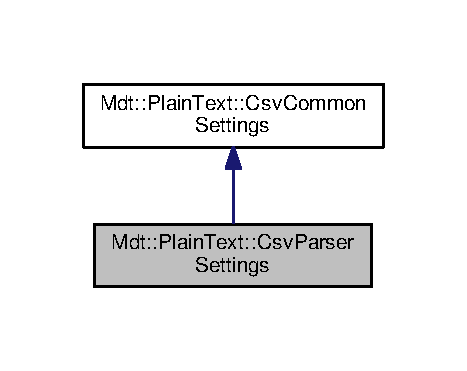
\includegraphics[width=224pt]{class_mdt_1_1_plain_text_1_1_csv_parser_settings__inherit__graph}
\end{center}
\end{figure}


Collaboration diagram for Mdt\+:\+:Plain\+Text\+:\+:Csv\+Parser\+Settings\+:\nopagebreak
\begin{figure}[H]
\begin{center}
\leavevmode
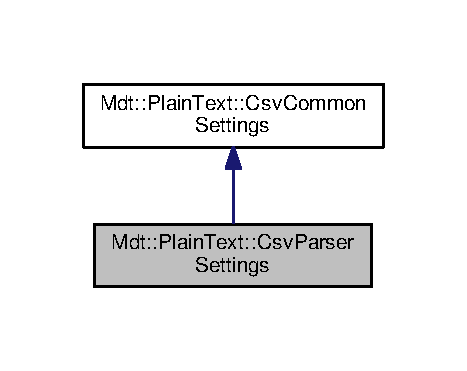
\includegraphics[width=224pt]{class_mdt_1_1_plain_text_1_1_csv_parser_settings__coll__graph}
\end{center}
\end{figure}
\subsection*{Public Member Functions}
\begin{DoxyCompactItemize}
\item 
\hyperlink{class_mdt_1_1_plain_text_1_1_csv_parser_settings_a478e33bc5b599b9f37e51e7932ca7089}{Csv\+Parser\+Settings} ()\hypertarget{class_mdt_1_1_plain_text_1_1_csv_parser_settings_a478e33bc5b599b9f37e51e7932ca7089}{}\label{class_mdt_1_1_plain_text_1_1_csv_parser_settings_a478e33bc5b599b9f37e51e7932ca7089}

\begin{DoxyCompactList}\small\item\em Construct default settings. \end{DoxyCompactList}\item 
\hyperlink{class_mdt_1_1_plain_text_1_1_csv_parser_settings_a13d6b4aa193caa6626577eaebac51028}{Csv\+Parser\+Settings} (const \hyperlink{class_mdt_1_1_plain_text_1_1_csv_parser_settings}{Csv\+Parser\+Settings} \&other)=default\hypertarget{class_mdt_1_1_plain_text_1_1_csv_parser_settings_a13d6b4aa193caa6626577eaebac51028}{}\label{class_mdt_1_1_plain_text_1_1_csv_parser_settings_a13d6b4aa193caa6626577eaebac51028}

\begin{DoxyCompactList}\small\item\em Construct settings as a copy of {\itshape other}. \end{DoxyCompactList}\item 
\hyperlink{class_mdt_1_1_plain_text_1_1_csv_parser_settings}{Csv\+Parser\+Settings} \& \hyperlink{class_mdt_1_1_plain_text_1_1_csv_parser_settings_a6755c057e7d04afb0cab6bcaa3ffb652}{operator=} (const \hyperlink{class_mdt_1_1_plain_text_1_1_csv_parser_settings}{Csv\+Parser\+Settings} \&other)=default\hypertarget{class_mdt_1_1_plain_text_1_1_csv_parser_settings_a6755c057e7d04afb0cab6bcaa3ffb652}{}\label{class_mdt_1_1_plain_text_1_1_csv_parser_settings_a6755c057e7d04afb0cab6bcaa3ffb652}

\begin{DoxyCompactList}\small\item\em Construct settings as a copy of {\itshape other}. \end{DoxyCompactList}\item 
\hyperlink{class_mdt_1_1_plain_text_1_1_csv_parser_settings_a88ebdf75dc028676bda13c37a437aad2}{Csv\+Parser\+Settings} (\hyperlink{class_mdt_1_1_plain_text_1_1_csv_parser_settings}{Csv\+Parser\+Settings} \&\&other)=default\hypertarget{class_mdt_1_1_plain_text_1_1_csv_parser_settings_a88ebdf75dc028676bda13c37a437aad2}{}\label{class_mdt_1_1_plain_text_1_1_csv_parser_settings_a88ebdf75dc028676bda13c37a437aad2}

\begin{DoxyCompactList}\small\item\em Construct settings as a copy of {\itshape other}. \end{DoxyCompactList}\item 
\hyperlink{class_mdt_1_1_plain_text_1_1_csv_parser_settings}{Csv\+Parser\+Settings} \& \hyperlink{class_mdt_1_1_plain_text_1_1_csv_parser_settings_a1d46a0ea41d380b8db95cb9d95c2190b}{operator=} (\hyperlink{class_mdt_1_1_plain_text_1_1_csv_parser_settings}{Csv\+Parser\+Settings} \&\&other)=default\hypertarget{class_mdt_1_1_plain_text_1_1_csv_parser_settings_a1d46a0ea41d380b8db95cb9d95c2190b}{}\label{class_mdt_1_1_plain_text_1_1_csv_parser_settings_a1d46a0ea41d380b8db95cb9d95c2190b}

\begin{DoxyCompactList}\small\item\em Construct settings as a copy of {\itshape other}. \end{DoxyCompactList}\item 
void \hyperlink{class_mdt_1_1_plain_text_1_1_csv_parser_settings_abe60d57922026d9de7a6e8d55511819e}{set\+Parse\+Exp} (bool parse)
\begin{DoxyCompactList}\small\item\em Set if Excel protection marker will be parsed. \end{DoxyCompactList}\item 
bool \hyperlink{class_mdt_1_1_plain_text_1_1_csv_parser_settings_af40bd9b66e5bec47230ece1cba3ee16a}{parse\+Exp} () const 
\begin{DoxyCompactList}\small\item\em Check if Excel protection marker will be parsed. \end{DoxyCompactList}\item 
bool \hyperlink{class_mdt_1_1_plain_text_1_1_csv_parser_settings_adf3ffeee7f6a9b5ba12108ee859ad0ce}{is\+Valid} () const 
\begin{DoxyCompactList}\small\item\em Check if settings are valid. \end{DoxyCompactList}\item 
void \hyperlink{class_mdt_1_1_plain_text_1_1_csv_parser_settings_a608d99bfe1f6777a8ff2b797d3b16931}{clear} ()
\begin{DoxyCompactList}\small\item\em Clear. \end{DoxyCompactList}\end{DoxyCompactItemize}


\subsection{Detailed Description}
C\+SV parser settings. 

Definition at line 31 of file Csv\+Parser\+Settings.\+h.



\subsection{Member Function Documentation}
\index{Mdt\+::\+Plain\+Text\+::\+Csv\+Parser\+Settings@{Mdt\+::\+Plain\+Text\+::\+Csv\+Parser\+Settings}!clear@{clear}}
\index{clear@{clear}!Mdt\+::\+Plain\+Text\+::\+Csv\+Parser\+Settings@{Mdt\+::\+Plain\+Text\+::\+Csv\+Parser\+Settings}}
\subsubsection[{\texorpdfstring{clear()}{clear()}}]{\setlength{\rightskip}{0pt plus 5cm}void Mdt\+::\+Plain\+Text\+::\+Csv\+Parser\+Settings\+::clear (
\begin{DoxyParamCaption}
{}
\end{DoxyParamCaption}
)}\hypertarget{class_mdt_1_1_plain_text_1_1_csv_parser_settings_a608d99bfe1f6777a8ff2b797d3b16931}{}\label{class_mdt_1_1_plain_text_1_1_csv_parser_settings_a608d99bfe1f6777a8ff2b797d3b16931}


Clear. 

Will reset to default settings. 

Definition at line 57 of file Csv\+Parser\+Settings.\+cpp.

\index{Mdt\+::\+Plain\+Text\+::\+Csv\+Parser\+Settings@{Mdt\+::\+Plain\+Text\+::\+Csv\+Parser\+Settings}!is\+Valid@{is\+Valid}}
\index{is\+Valid@{is\+Valid}!Mdt\+::\+Plain\+Text\+::\+Csv\+Parser\+Settings@{Mdt\+::\+Plain\+Text\+::\+Csv\+Parser\+Settings}}
\subsubsection[{\texorpdfstring{is\+Valid() const }{isValid() const }}]{\setlength{\rightskip}{0pt plus 5cm}bool Mdt\+::\+Plain\+Text\+::\+Csv\+Parser\+Settings\+::is\+Valid (
\begin{DoxyParamCaption}
{}
\end{DoxyParamCaption}
) const}\hypertarget{class_mdt_1_1_plain_text_1_1_csv_parser_settings_adf3ffeee7f6a9b5ba12108ee859ad0ce}{}\label{class_mdt_1_1_plain_text_1_1_csv_parser_settings_adf3ffeee7f6a9b5ba12108ee859ad0ce}


Check if settings are valid. 

If this settings is not valid, use last\+Error() to get what is wrong. 

Definition at line 34 of file Csv\+Parser\+Settings.\+cpp.

\index{Mdt\+::\+Plain\+Text\+::\+Csv\+Parser\+Settings@{Mdt\+::\+Plain\+Text\+::\+Csv\+Parser\+Settings}!parse\+Exp@{parse\+Exp}}
\index{parse\+Exp@{parse\+Exp}!Mdt\+::\+Plain\+Text\+::\+Csv\+Parser\+Settings@{Mdt\+::\+Plain\+Text\+::\+Csv\+Parser\+Settings}}
\subsubsection[{\texorpdfstring{parse\+Exp() const }{parseExp() const }}]{\setlength{\rightskip}{0pt plus 5cm}bool Mdt\+::\+Plain\+Text\+::\+Csv\+Parser\+Settings\+::parse\+Exp (
\begin{DoxyParamCaption}
{}
\end{DoxyParamCaption}
) const\hspace{0.3cm}{\ttfamily [inline]}}\hypertarget{class_mdt_1_1_plain_text_1_1_csv_parser_settings_af40bd9b66e5bec47230ece1cba3ee16a}{}\label{class_mdt_1_1_plain_text_1_1_csv_parser_settings_af40bd9b66e5bec47230ece1cba3ee16a}


Check if Excel protection marker will be parsed. 

The Excel protection marker (E\+XP) is explained in C\+S\+V-\/1203 standard, §10.

When parse\+Exp is true, when a field begins with a $\sim$ (=E\+XP), it will not be stored in resulting data.

The ability to not parse E\+XP is a non standard extention.

\begin{DoxySeeAlso}{See also}
\hyperlink{class_mdt_1_1_plain_text_1_1_csv_parser_settings_abe60d57922026d9de7a6e8d55511819e}{set\+Parse\+Exp()} 
\end{DoxySeeAlso}


Definition at line 79 of file Csv\+Parser\+Settings.\+h.

\index{Mdt\+::\+Plain\+Text\+::\+Csv\+Parser\+Settings@{Mdt\+::\+Plain\+Text\+::\+Csv\+Parser\+Settings}!set\+Parse\+Exp@{set\+Parse\+Exp}}
\index{set\+Parse\+Exp@{set\+Parse\+Exp}!Mdt\+::\+Plain\+Text\+::\+Csv\+Parser\+Settings@{Mdt\+::\+Plain\+Text\+::\+Csv\+Parser\+Settings}}
\subsubsection[{\texorpdfstring{set\+Parse\+Exp(bool parse)}{setParseExp(bool parse)}}]{\setlength{\rightskip}{0pt plus 5cm}void Mdt\+::\+Plain\+Text\+::\+Csv\+Parser\+Settings\+::set\+Parse\+Exp (
\begin{DoxyParamCaption}
\item[{bool}]{parse}
\end{DoxyParamCaption}
)}\hypertarget{class_mdt_1_1_plain_text_1_1_csv_parser_settings_abe60d57922026d9de7a6e8d55511819e}{}\label{class_mdt_1_1_plain_text_1_1_csv_parser_settings_abe60d57922026d9de7a6e8d55511819e}


Set if Excel protection marker will be parsed. 

\begin{DoxySeeAlso}{See also}
\hyperlink{class_mdt_1_1_plain_text_1_1_csv_parser_settings_af40bd9b66e5bec47230ece1cba3ee16a}{parse\+Exp()} 
\end{DoxySeeAlso}


Definition at line 29 of file Csv\+Parser\+Settings.\+cpp.



The documentation for this class was generated from the following files\+:\begin{DoxyCompactItemize}
\item 
libs/\+Plain\+Text\+\_\+\+Core/src/\+Mdt/\+Plain\+Text/Csv\+Parser\+Settings.\+h\item 
libs/\+Plain\+Text\+\_\+\+Core/src/\+Mdt/\+Plain\+Text/Csv\+Parser\+Settings.\+cpp\end{DoxyCompactItemize}

\hypertarget{class_mdt_1_1_plain_text_1_1_csv_parser_template}{}\section{Mdt\+:\+:Plain\+Text\+:\+:Csv\+Parser\+Template$<$ Source\+Iterator $>$ Class Template Reference}
\label{class_mdt_1_1_plain_text_1_1_csv_parser_template}\index{Mdt\+::\+Plain\+Text\+::\+Csv\+Parser\+Template$<$ Source\+Iterator $>$@{Mdt\+::\+Plain\+Text\+::\+Csv\+Parser\+Template$<$ Source\+Iterator $>$}}


C\+SV parser template.  




{\ttfamily \#include $<$Csv\+Parser\+Template.\+h$>$}



Inheritance diagram for Mdt\+:\+:Plain\+Text\+:\+:Csv\+Parser\+Template$<$ Source\+Iterator $>$\+:
\nopagebreak
\begin{figure}[H]
\begin{center}
\leavevmode
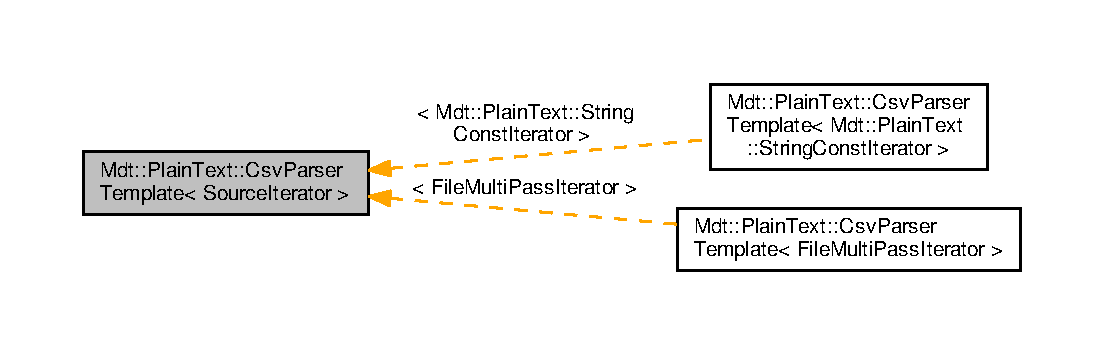
\includegraphics[width=350pt]{class_mdt_1_1_plain_text_1_1_csv_parser_template__inherit__graph}
\end{center}
\end{figure}
\subsection*{Public Member Functions}
\begin{DoxyCompactItemize}
\item 
\hyperlink{class_mdt_1_1_plain_text_1_1_csv_parser_template_a0365862918b7ffb5e70bfd2fd6a0e95e}{Csv\+Parser\+Template} ()=default
\begin{DoxyCompactList}\small\item\em Default constructor. \end{DoxyCompactList}\item 
{\bfseries Csv\+Parser\+Template} (const \hyperlink{class_mdt_1_1_plain_text_1_1_csv_parser_template}{Csv\+Parser\+Template} \&)=delete\hypertarget{class_mdt_1_1_plain_text_1_1_csv_parser_template_a50df2d2fb8eda54bf9ec1dced98013e3}{}\label{class_mdt_1_1_plain_text_1_1_csv_parser_template_a50df2d2fb8eda54bf9ec1dced98013e3}

\item 
\hyperlink{class_mdt_1_1_plain_text_1_1_csv_parser_template}{Csv\+Parser\+Template} \& {\bfseries operator=} (const \hyperlink{class_mdt_1_1_plain_text_1_1_csv_parser_template}{Csv\+Parser\+Template} \&)=delete\hypertarget{class_mdt_1_1_plain_text_1_1_csv_parser_template_a231614b1287419ebd121c7909802f1a7}{}\label{class_mdt_1_1_plain_text_1_1_csv_parser_template_a231614b1287419ebd121c7909802f1a7}

\item 
{\bfseries Csv\+Parser\+Template} (\hyperlink{class_mdt_1_1_plain_text_1_1_csv_parser_template}{Csv\+Parser\+Template} \&\&)=delete\hypertarget{class_mdt_1_1_plain_text_1_1_csv_parser_template_af7d085875af2f5244958e0cb06daf39b}{}\label{class_mdt_1_1_plain_text_1_1_csv_parser_template_af7d085875af2f5244958e0cb06daf39b}

\item 
\hyperlink{class_mdt_1_1_plain_text_1_1_csv_parser_template}{Csv\+Parser\+Template} \& {\bfseries operator=} (\hyperlink{class_mdt_1_1_plain_text_1_1_csv_parser_template}{Csv\+Parser\+Template} \&\&)=delete\hypertarget{class_mdt_1_1_plain_text_1_1_csv_parser_template_aa7bfc2bddc9d3ae6690d741c2a24550d}{}\label{class_mdt_1_1_plain_text_1_1_csv_parser_template_aa7bfc2bddc9d3ae6690d741c2a24550d}

\item 
void \hyperlink{class_mdt_1_1_plain_text_1_1_csv_parser_template_a95c35ee9721efec0aedcf8b18b310001}{setup\+Parser} (const \hyperlink{class_mdt_1_1_plain_text_1_1_csv_parser_settings}{Csv\+Parser\+Settings} \&settings)
\begin{DoxyCompactList}\small\item\em Setup parser. \end{DoxyCompactList}\item 
bool \hyperlink{class_mdt_1_1_plain_text_1_1_csv_parser_template_a215191b75041f462135572f328669731}{is\+Valid} () const 
\begin{DoxyCompactList}\small\item\em Check if parser is valid. \end{DoxyCompactList}\item 
\hyperlink{class_mdt_1_1_expected}{Mdt\+::\+Expected}$<$ String\+Record $>$ \hyperlink{class_mdt_1_1_plain_text_1_1_csv_parser_template_aa6a88c11fa8def4ee7fd3437d9099a95}{read\+Line} (Source\+Iterator \&first, const Source\+Iterator \&last)
\begin{DoxyCompactList}\small\item\em Read one line of C\+SV data. \end{DoxyCompactList}\end{DoxyCompactItemize}


\subsection{Detailed Description}
\subsubsection*{template$<$typename Source\+Iterator$>$\\*
class Mdt\+::\+Plain\+Text\+::\+Csv\+Parser\+Template$<$ Source\+Iterator $>$}

C\+SV parser template. 

This class implements the parser logic, and can act on different input containers that have S\+TL compatible iterators.


\begin{DoxyTemplParams}{Template Parameters}
{\em Source\+Iterator} & Type of iterator that will act on the source. \\
\hline
\end{DoxyTemplParams}
\begin{DoxyNote}{Note}
Including directly this header in a project can slow down compilation time 
\end{DoxyNote}
\begin{DoxySeeAlso}{See also}
\hyperlink{class_mdt_1_1_plain_text_1_1_csv_string_parser}{Csv\+String\+Parser} 

\hyperlink{class_mdt_1_1_plain_text_1_1_csv_file_parser}{Csv\+File\+Parser} 
\end{DoxySeeAlso}
\begin{DoxyNote}{Note}
Some part of this A\+PI documentation refers to following standards\+: \begin{DoxyItemize}
\item C\+S\+V-\/1203 available here\+: \href{http://mastpoint.com/csv-1203}{\tt http\+://mastpoint.\+com/csv-\/1203} \item R\+FC 4180 available here\+: \href{https://tools.ietf.org/html/rfc4180}{\tt https\+://tools.\+ietf.\+org/html/rfc4180} \end{DoxyItemize}

\end{DoxyNote}


Definition at line 40 of file Csv\+File\+Parser.\+h.



\subsection{Constructor \& Destructor Documentation}
\index{Mdt\+::\+Plain\+Text\+::\+Csv\+Parser\+Template@{Mdt\+::\+Plain\+Text\+::\+Csv\+Parser\+Template}!Csv\+Parser\+Template@{Csv\+Parser\+Template}}
\index{Csv\+Parser\+Template@{Csv\+Parser\+Template}!Mdt\+::\+Plain\+Text\+::\+Csv\+Parser\+Template@{Mdt\+::\+Plain\+Text\+::\+Csv\+Parser\+Template}}
\subsubsection[{\texorpdfstring{Csv\+Parser\+Template()=default}{CsvParserTemplate()=default}}]{\setlength{\rightskip}{0pt plus 5cm}template$<$typename Source\+Iterator$>$ {\bf Mdt\+::\+Plain\+Text\+::\+Csv\+Parser\+Template}$<$ Source\+Iterator $>$\+::{\bf Csv\+Parser\+Template} (
\begin{DoxyParamCaption}
{}
\end{DoxyParamCaption}
)\hspace{0.3cm}{\ttfamily [default]}}\hypertarget{class_mdt_1_1_plain_text_1_1_csv_parser_template_a0365862918b7ffb5e70bfd2fd6a0e95e}{}\label{class_mdt_1_1_plain_text_1_1_csv_parser_template_a0365862918b7ffb5e70bfd2fd6a0e95e}


Default constructor. 



\subsection{Member Function Documentation}
\index{Mdt\+::\+Plain\+Text\+::\+Csv\+Parser\+Template@{Mdt\+::\+Plain\+Text\+::\+Csv\+Parser\+Template}!is\+Valid@{is\+Valid}}
\index{is\+Valid@{is\+Valid}!Mdt\+::\+Plain\+Text\+::\+Csv\+Parser\+Template@{Mdt\+::\+Plain\+Text\+::\+Csv\+Parser\+Template}}
\subsubsection[{\texorpdfstring{is\+Valid() const }{isValid() const }}]{\setlength{\rightskip}{0pt plus 5cm}template$<$typename Source\+Iterator$>$ bool {\bf Mdt\+::\+Plain\+Text\+::\+Csv\+Parser\+Template}$<$ Source\+Iterator $>$\+::is\+Valid (
\begin{DoxyParamCaption}
{}
\end{DoxyParamCaption}
) const\hspace{0.3cm}{\ttfamily [inline]}}\hypertarget{class_mdt_1_1_plain_text_1_1_csv_parser_template_a215191b75041f462135572f328669731}{}\label{class_mdt_1_1_plain_text_1_1_csv_parser_template_a215191b75041f462135572f328669731}


Check if parser is valid. 

Parser is valid once \hyperlink{class_mdt_1_1_plain_text_1_1_csv_parser_template_a95c35ee9721efec0aedcf8b18b310001}{setup\+Parser()} was called at least once 

Definition at line 146 of file Csv\+Parser\+Template.\+h.

\index{Mdt\+::\+Plain\+Text\+::\+Csv\+Parser\+Template@{Mdt\+::\+Plain\+Text\+::\+Csv\+Parser\+Template}!read\+Line@{read\+Line}}
\index{read\+Line@{read\+Line}!Mdt\+::\+Plain\+Text\+::\+Csv\+Parser\+Template@{Mdt\+::\+Plain\+Text\+::\+Csv\+Parser\+Template}}
\subsubsection[{\texorpdfstring{read\+Line(\+Source\+Iterator \&first, const Source\+Iterator \&last)}{readLine(SourceIterator &first, const SourceIterator &last)}}]{\setlength{\rightskip}{0pt plus 5cm}template$<$typename Source\+Iterator$>$ {\bf Mdt\+::\+Expected}$<$String\+Record$>$ {\bf Mdt\+::\+Plain\+Text\+::\+Csv\+Parser\+Template}$<$ Source\+Iterator $>$\+::read\+Line (
\begin{DoxyParamCaption}
\item[{Source\+Iterator \&}]{first, }
\item[{const Source\+Iterator \&}]{last}
\end{DoxyParamCaption}
)\hspace{0.3cm}{\ttfamily [inline]}}\hypertarget{class_mdt_1_1_plain_text_1_1_csv_parser_template_aa6a88c11fa8def4ee7fd3437d9099a95}{}\label{class_mdt_1_1_plain_text_1_1_csv_parser_template_aa6a88c11fa8def4ee7fd3437d9099a95}


Read one line of C\+SV data. 

\begin{DoxyPrecond}{Precondition}
\hyperlink{class_mdt_1_1_plain_text_1_1_csv_parser_template_a95c35ee9721efec0aedcf8b18b310001}{setup\+Parser()} must be called at least once before 
\end{DoxyPrecond}


Definition at line 155 of file Csv\+Parser\+Template.\+h.

\index{Mdt\+::\+Plain\+Text\+::\+Csv\+Parser\+Template@{Mdt\+::\+Plain\+Text\+::\+Csv\+Parser\+Template}!setup\+Parser@{setup\+Parser}}
\index{setup\+Parser@{setup\+Parser}!Mdt\+::\+Plain\+Text\+::\+Csv\+Parser\+Template@{Mdt\+::\+Plain\+Text\+::\+Csv\+Parser\+Template}}
\subsubsection[{\texorpdfstring{setup\+Parser(const Csv\+Parser\+Settings \&settings)}{setupParser(const CsvParserSettings &settings)}}]{\setlength{\rightskip}{0pt plus 5cm}template$<$typename Source\+Iterator$>$ void {\bf Mdt\+::\+Plain\+Text\+::\+Csv\+Parser\+Template}$<$ Source\+Iterator $>$\+::setup\+Parser (
\begin{DoxyParamCaption}
\item[{const {\bf Csv\+Parser\+Settings} \&}]{settings}
\end{DoxyParamCaption}
)\hspace{0.3cm}{\ttfamily [inline]}}\hypertarget{class_mdt_1_1_plain_text_1_1_csv_parser_template_a95c35ee9721efec0aedcf8b18b310001}{}\label{class_mdt_1_1_plain_text_1_1_csv_parser_template_a95c35ee9721efec0aedcf8b18b310001}


Setup parser. 

\begin{DoxyPrecond}{Precondition}
{\itshape settings} must be valid 
\end{DoxyPrecond}


Definition at line 78 of file Csv\+Parser\+Template.\+h.



The documentation for this class was generated from the following files\+:\begin{DoxyCompactItemize}
\item 
libs/\+Plain\+Text\+\_\+\+Core/src/\+Mdt/\+Plain\+Text/Csv\+File\+Parser.\+h\item 
libs/\+Plain\+Text\+\_\+\+Core/src/\+Mdt/\+Plain\+Text/Csv\+Parser\+Template.\+h\end{DoxyCompactItemize}

\hypertarget{class_mdt_1_1_plain_text_1_1_csv_string_parser}{}\section{Mdt\+:\+:Plain\+Text\+:\+:Csv\+String\+Parser Class Reference}
\label{class_mdt_1_1_plain_text_1_1_csv_string_parser}\index{Mdt\+::\+Plain\+Text\+::\+Csv\+String\+Parser@{Mdt\+::\+Plain\+Text\+::\+Csv\+String\+Parser}}


C\+SV parser that acts on a Q\+String as input.  




{\ttfamily \#include $<$Csv\+String\+Parser.\+h$>$}

\subsection*{Public Member Functions}
\begin{DoxyCompactItemize}
\item 
\hyperlink{class_mdt_1_1_plain_text_1_1_csv_string_parser_a5a6afeedd8f074afe78fd5f161a06140}{Csv\+String\+Parser} ()
\begin{DoxyCompactList}\small\item\em Default constructor. \end{DoxyCompactList}\item 
void \hyperlink{class_mdt_1_1_plain_text_1_1_csv_string_parser_a30af818bc2d40ac11e29562e2dd19108}{set\+Csv\+Settings} (const \hyperlink{class_mdt_1_1_plain_text_1_1_csv_parser_settings}{Csv\+Parser\+Settings} \&settings)
\begin{DoxyCompactList}\small\item\em Set C\+SV settings. \end{DoxyCompactList}\item 
void \hyperlink{class_mdt_1_1_plain_text_1_1_csv_string_parser_a671b38b46afd066a71677b7cdebdc154}{set\+Source} (const Q\+String \&source)
\begin{DoxyCompactList}\small\item\em Set C\+SV source string. \end{DoxyCompactList}\item 
bool \hyperlink{class_mdt_1_1_plain_text_1_1_csv_string_parser_a81d09c21ee3fdbc499e584d799e3a3ab}{at\+End} () const 
\begin{DoxyCompactList}\small\item\em Check if parser is at end of the source. \end{DoxyCompactList}\item 
\hyperlink{class_mdt_1_1_expected}{Mdt\+::\+Expected}$<$ String\+Record $>$ \hyperlink{class_mdt_1_1_plain_text_1_1_csv_string_parser_a4089cbf5a42d66903247c4bd5633e3fb}{read\+Line} ()
\begin{DoxyCompactList}\small\item\em Read one line. \end{DoxyCompactList}\item 
\hyperlink{class_mdt_1_1_expected}{Mdt\+::\+Expected}$<$ String\+Record\+List $>$ \hyperlink{class_mdt_1_1_plain_text_1_1_csv_string_parser_a9bed7245aaadf05eccc231df11a7a9e1}{read\+All} ()
\begin{DoxyCompactList}\small\item\em Read the entire C\+SV string. \end{DoxyCompactList}\end{DoxyCompactItemize}


\subsection{Detailed Description}
C\+SV parser that acts on a Q\+String as input. 

\hyperlink{class_mdt_1_1_plain_text_1_1_csv_string_parser}{Csv\+String\+Parser} parses a C\+SV string. The C\+SV string can contain quoted section.

\begin{DoxyNote}{Note}
Some part of this A\+PI documentation refers to following standards\+: \begin{DoxyItemize}
\item C\+S\+V-\/1203 available here\+: \href{http://mastpoint.com/csv-1203}{\tt http\+://mastpoint.\+com/csv-\/1203} \item R\+FC 4180 available here\+: \href{https://tools.ietf.org/html/rfc4180}{\tt https\+://tools.\+ietf.\+org/html/rfc4180} \end{DoxyItemize}

\end{DoxyNote}


Definition at line 46 of file Csv\+String\+Parser.\+h.



\subsection{Constructor \& Destructor Documentation}
\index{Mdt\+::\+Plain\+Text\+::\+Csv\+String\+Parser@{Mdt\+::\+Plain\+Text\+::\+Csv\+String\+Parser}!Csv\+String\+Parser@{Csv\+String\+Parser}}
\index{Csv\+String\+Parser@{Csv\+String\+Parser}!Mdt\+::\+Plain\+Text\+::\+Csv\+String\+Parser@{Mdt\+::\+Plain\+Text\+::\+Csv\+String\+Parser}}
\subsubsection[{\texorpdfstring{Csv\+String\+Parser()}{CsvStringParser()}}]{\setlength{\rightskip}{0pt plus 5cm}Mdt\+::\+Plain\+Text\+::\+Csv\+String\+Parser\+::\+Csv\+String\+Parser (
\begin{DoxyParamCaption}
{}
\end{DoxyParamCaption}
)}\hypertarget{class_mdt_1_1_plain_text_1_1_csv_string_parser_a5a6afeedd8f074afe78fd5f161a06140}{}\label{class_mdt_1_1_plain_text_1_1_csv_string_parser_a5a6afeedd8f074afe78fd5f161a06140}


Default constructor. 



Definition at line 26 of file Csv\+String\+Parser.\+cpp.



\subsection{Member Function Documentation}
\index{Mdt\+::\+Plain\+Text\+::\+Csv\+String\+Parser@{Mdt\+::\+Plain\+Text\+::\+Csv\+String\+Parser}!at\+End@{at\+End}}
\index{at\+End@{at\+End}!Mdt\+::\+Plain\+Text\+::\+Csv\+String\+Parser@{Mdt\+::\+Plain\+Text\+::\+Csv\+String\+Parser}}
\subsubsection[{\texorpdfstring{at\+End() const }{atEnd() const }}]{\setlength{\rightskip}{0pt plus 5cm}bool Mdt\+::\+Plain\+Text\+::\+Csv\+String\+Parser\+::at\+End (
\begin{DoxyParamCaption}
{}
\end{DoxyParamCaption}
) const}\hypertarget{class_mdt_1_1_plain_text_1_1_csv_string_parser_a81d09c21ee3fdbc499e584d799e3a3ab}{}\label{class_mdt_1_1_plain_text_1_1_csv_string_parser_a81d09c21ee3fdbc499e584d799e3a3ab}


Check if parser is at end of the source. 



Definition at line 48 of file Csv\+String\+Parser.\+cpp.

\index{Mdt\+::\+Plain\+Text\+::\+Csv\+String\+Parser@{Mdt\+::\+Plain\+Text\+::\+Csv\+String\+Parser}!read\+All@{read\+All}}
\index{read\+All@{read\+All}!Mdt\+::\+Plain\+Text\+::\+Csv\+String\+Parser@{Mdt\+::\+Plain\+Text\+::\+Csv\+String\+Parser}}
\subsubsection[{\texorpdfstring{read\+All()}{readAll()}}]{\setlength{\rightskip}{0pt plus 5cm}{\bf Expected}$<$ String\+Record\+List $>$ Mdt\+::\+Plain\+Text\+::\+Csv\+String\+Parser\+::read\+All (
\begin{DoxyParamCaption}
{}
\end{DoxyParamCaption}
)}\hypertarget{class_mdt_1_1_plain_text_1_1_csv_string_parser_a9bed7245aaadf05eccc231df11a7a9e1}{}\label{class_mdt_1_1_plain_text_1_1_csv_string_parser_a9bed7245aaadf05eccc231df11a7a9e1}


Read the entire C\+SV string. 

\begin{DoxyPrecond}{Precondition}
C\+SV settings must be set before calling this function 
\end{DoxyPrecond}
\begin{DoxySeeAlso}{See also}
\hyperlink{class_mdt_1_1_plain_text_1_1_csv_string_parser_a30af818bc2d40ac11e29562e2dd19108}{set\+Csv\+Settings()} 
\end{DoxySeeAlso}


Definition at line 60 of file Csv\+String\+Parser.\+cpp.

\index{Mdt\+::\+Plain\+Text\+::\+Csv\+String\+Parser@{Mdt\+::\+Plain\+Text\+::\+Csv\+String\+Parser}!read\+Line@{read\+Line}}
\index{read\+Line@{read\+Line}!Mdt\+::\+Plain\+Text\+::\+Csv\+String\+Parser@{Mdt\+::\+Plain\+Text\+::\+Csv\+String\+Parser}}
\subsubsection[{\texorpdfstring{read\+Line()}{readLine()}}]{\setlength{\rightskip}{0pt plus 5cm}{\bf Expected}$<$ String\+Record $>$ Mdt\+::\+Plain\+Text\+::\+Csv\+String\+Parser\+::read\+Line (
\begin{DoxyParamCaption}
{}
\end{DoxyParamCaption}
)}\hypertarget{class_mdt_1_1_plain_text_1_1_csv_string_parser_a4089cbf5a42d66903247c4bd5633e3fb}{}\label{class_mdt_1_1_plain_text_1_1_csv_string_parser_a4089cbf5a42d66903247c4bd5633e3fb}


Read one line. 

If a end of line is in a quoted section, it will not be threated as end of line.

This function can be used, f.\+ex., to store a long string to some other storage device, without having to copy the entiere source before. Reading line by line can also save some memory.

\begin{DoxyPrecond}{Precondition}
C\+SV settings must be set before calling this function 
\end{DoxyPrecond}
\begin{DoxySeeAlso}{See also}
\hyperlink{class_mdt_1_1_plain_text_1_1_csv_string_parser_a30af818bc2d40ac11e29562e2dd19108}{set\+Csv\+Settings()} 
\end{DoxySeeAlso}


Definition at line 53 of file Csv\+String\+Parser.\+cpp.

\index{Mdt\+::\+Plain\+Text\+::\+Csv\+String\+Parser@{Mdt\+::\+Plain\+Text\+::\+Csv\+String\+Parser}!set\+Csv\+Settings@{set\+Csv\+Settings}}
\index{set\+Csv\+Settings@{set\+Csv\+Settings}!Mdt\+::\+Plain\+Text\+::\+Csv\+String\+Parser@{Mdt\+::\+Plain\+Text\+::\+Csv\+String\+Parser}}
\subsubsection[{\texorpdfstring{set\+Csv\+Settings(const Csv\+Parser\+Settings \&settings)}{setCsvSettings(const CsvParserSettings &settings)}}]{\setlength{\rightskip}{0pt plus 5cm}void Mdt\+::\+Plain\+Text\+::\+Csv\+String\+Parser\+::set\+Csv\+Settings (
\begin{DoxyParamCaption}
\item[{const {\bf Csv\+Parser\+Settings} \&}]{settings}
\end{DoxyParamCaption}
)}\hypertarget{class_mdt_1_1_plain_text_1_1_csv_string_parser_a30af818bc2d40ac11e29562e2dd19108}{}\label{class_mdt_1_1_plain_text_1_1_csv_string_parser_a30af818bc2d40ac11e29562e2dd19108}


Set C\+SV settings. 

\begin{DoxyPrecond}{Precondition}
{\itshape settings} must be valid 
\end{DoxyPrecond}


Definition at line 35 of file Csv\+String\+Parser.\+cpp.

\index{Mdt\+::\+Plain\+Text\+::\+Csv\+String\+Parser@{Mdt\+::\+Plain\+Text\+::\+Csv\+String\+Parser}!set\+Source@{set\+Source}}
\index{set\+Source@{set\+Source}!Mdt\+::\+Plain\+Text\+::\+Csv\+String\+Parser@{Mdt\+::\+Plain\+Text\+::\+Csv\+String\+Parser}}
\subsubsection[{\texorpdfstring{set\+Source(const Q\+String \&source)}{setSource(const QString &source)}}]{\setlength{\rightskip}{0pt plus 5cm}void Mdt\+::\+Plain\+Text\+::\+Csv\+String\+Parser\+::set\+Source (
\begin{DoxyParamCaption}
\item[{const Q\+String \&}]{source}
\end{DoxyParamCaption}
)}\hypertarget{class_mdt_1_1_plain_text_1_1_csv_string_parser_a671b38b46afd066a71677b7cdebdc154}{}\label{class_mdt_1_1_plain_text_1_1_csv_string_parser_a671b38b46afd066a71677b7cdebdc154}


Set C\+SV source string. 

\begin{DoxyNote}{Note}
Parsing will be done directly on source Make shure that it is not modified during parsing process (take a look at Qt documentation about S\+TL style iterators invalidation for details) 
\end{DoxyNote}


Definition at line 42 of file Csv\+String\+Parser.\+cpp.



The documentation for this class was generated from the following files\+:\begin{DoxyCompactItemize}
\item 
libs/\+Plain\+Text\+\_\+\+Core/src/\+Mdt/\+Plain\+Text/Csv\+String\+Parser.\+h\item 
libs/\+Plain\+Text\+\_\+\+Core/src/\+Mdt/\+Plain\+Text/Csv\+String\+Parser.\+cpp\end{DoxyCompactItemize}

\hypertarget{class_mdt_1_1_numeric_1_1_double}{}\section{Mdt\+:\+:Numeric\+:\+:Double Class Reference}
\label{class_mdt_1_1_numeric_1_1_double}\index{Mdt\+::\+Numeric\+::\+Double@{Mdt\+::\+Numeric\+::\+Double}}


Wraps floating (double) value with some helper functions.  




{\ttfamily \#include $<$Double.\+h$>$}

\subsection*{Public Member Functions}
\begin{DoxyCompactItemize}
\item 
constexpr \hyperlink{class_mdt_1_1_numeric_1_1_double_ae340e90c5924e4e38a6c79c4d6ebdd04}{Double} () noexcept\hypertarget{class_mdt_1_1_numeric_1_1_double_ae340e90c5924e4e38a6c79c4d6ebdd04}{}\label{class_mdt_1_1_numeric_1_1_double_ae340e90c5924e4e38a6c79c4d6ebdd04}

\begin{DoxyCompactList}\small\item\em Construct a null \hyperlink{class_mdt_1_1_numeric_1_1_double}{Double}. \end{DoxyCompactList}\item 
constexpr \hyperlink{class_mdt_1_1_numeric_1_1_double_a3d99ae951bf2716fe59c81e1efa5387a}{Double} (double x) noexcept\hypertarget{class_mdt_1_1_numeric_1_1_double_a3d99ae951bf2716fe59c81e1efa5387a}{}\label{class_mdt_1_1_numeric_1_1_double_a3d99ae951bf2716fe59c81e1efa5387a}

\begin{DoxyCompactList}\small\item\em Construct a \hyperlink{class_mdt_1_1_numeric_1_1_double}{Double} with a value. \end{DoxyCompactList}\item 
constexpr double \hyperlink{class_mdt_1_1_numeric_1_1_double_a962b13f89e149e5e7cec93405513479d}{to\+Double} () const noexcept
\begin{DoxyCompactList}\small\item\em Get \hyperlink{class_mdt_1_1_numeric_1_1_double}{Double} value. \end{DoxyCompactList}\item 
bool \hyperlink{class_mdt_1_1_numeric_1_1_double_a72129dd1dd50fdf7503091a3c5881d1a}{is\+Infinity} () const noexcept\hypertarget{class_mdt_1_1_numeric_1_1_double_a72129dd1dd50fdf7503091a3c5881d1a}{}\label{class_mdt_1_1_numeric_1_1_double_a72129dd1dd50fdf7503091a3c5881d1a}

\begin{DoxyCompactList}\small\item\em Check if value is infinity (+infinity or -\/infinity) \end{DoxyCompactList}\item 
constexpr void \hyperlink{class_mdt_1_1_numeric_1_1_double_aad324b42829414e760ca305f70a0a692}{set\+Minus\+Infinity} () noexcept\hypertarget{class_mdt_1_1_numeric_1_1_double_aad324b42829414e760ca305f70a0a692}{}\label{class_mdt_1_1_numeric_1_1_double_aad324b42829414e760ca305f70a0a692}

\begin{DoxyCompactList}\small\item\em Set -\/infinity. \end{DoxyCompactList}\item 
bool \hyperlink{class_mdt_1_1_numeric_1_1_double_a08fc926a071bfcda66e86b0081825b44}{is\+Minus\+Infinity} () const noexcept\hypertarget{class_mdt_1_1_numeric_1_1_double_a08fc926a071bfcda66e86b0081825b44}{}\label{class_mdt_1_1_numeric_1_1_double_a08fc926a071bfcda66e86b0081825b44}

\begin{DoxyCompactList}\small\item\em Check if value is -\/infinity. \end{DoxyCompactList}\item 
constexpr void \hyperlink{class_mdt_1_1_numeric_1_1_double_a922f39ec2ee308c7c86471252a22a28c}{set\+Plus\+Infinity} () noexcept\hypertarget{class_mdt_1_1_numeric_1_1_double_a922f39ec2ee308c7c86471252a22a28c}{}\label{class_mdt_1_1_numeric_1_1_double_a922f39ec2ee308c7c86471252a22a28c}

\begin{DoxyCompactList}\small\item\em Set +infinity. \end{DoxyCompactList}\item 
bool \hyperlink{class_mdt_1_1_numeric_1_1_double_aff0038f2052e0942cd7544097ccbe40a}{is\+Plus\+Infinity} () const noexcept\hypertarget{class_mdt_1_1_numeric_1_1_double_aff0038f2052e0942cd7544097ccbe40a}{}\label{class_mdt_1_1_numeric_1_1_double_aff0038f2052e0942cd7544097ccbe40a}

\begin{DoxyCompactList}\small\item\em Check if value is +infinity. \end{DoxyCompactList}\item 
bool \hyperlink{class_mdt_1_1_numeric_1_1_double_a2cc3d131c3558fc7d6b494c439e2f826}{is\+NaN} () const noexcept
\begin{DoxyCompactList}\small\item\em Check if value is NaN. \end{DoxyCompactList}\item 
bool \hyperlink{class_mdt_1_1_numeric_1_1_double_a01d4bfdb780a56d84fa07f48282aa254}{is\+Null} () const noexcept
\begin{DoxyCompactList}\small\item\em Check if \hyperlink{class_mdt_1_1_numeric_1_1_double}{Double} is null. \end{DoxyCompactList}\item 
constexpr void \hyperlink{class_mdt_1_1_numeric_1_1_double_a0306258c3934f174cbe9826f129e705a}{clear} () noexcept\hypertarget{class_mdt_1_1_numeric_1_1_double_a0306258c3934f174cbe9826f129e705a}{}\label{class_mdt_1_1_numeric_1_1_double_a0306258c3934f174cbe9826f129e705a}

\begin{DoxyCompactList}\small\item\em Clear. \end{DoxyCompactList}\item 
constexpr \hyperlink{class_mdt_1_1_numeric_1_1_double}{Double} \hyperlink{class_mdt_1_1_numeric_1_1_double_a833b6f2ba91fee3158b2e5eba5a978dc}{operator-\/} () const 
\begin{DoxyCompactList}\small\item\em Negation operator. \end{DoxyCompactList}\end{DoxyCompactItemize}
\subsection*{Friends}
\begin{DoxyCompactItemize}
\item 
bool \hyperlink{class_mdt_1_1_numeric_1_1_double_ae628a01068d337ab31665a46510d501b}{operator==} (const \hyperlink{class_mdt_1_1_numeric_1_1_double}{Double} \&x, const \hyperlink{class_mdt_1_1_numeric_1_1_double}{Double} \&y) noexcept
\begin{DoxyCompactList}\small\item\em Equality comparison operator. \end{DoxyCompactList}\item 
bool \hyperlink{class_mdt_1_1_numeric_1_1_double_a9f04aacec2f90c7849a50cee30ae2653}{operator!=} (const \hyperlink{class_mdt_1_1_numeric_1_1_double}{Double} \&x, const \hyperlink{class_mdt_1_1_numeric_1_1_double}{Double} \&y) noexcept
\begin{DoxyCompactList}\small\item\em Inequality comparison operator. \end{DoxyCompactList}\item 
bool \hyperlink{class_mdt_1_1_numeric_1_1_double_a1347b811297911998b12f4c310a1d177}{operator$<$} (const \hyperlink{class_mdt_1_1_numeric_1_1_double}{Double} \&x, const \hyperlink{class_mdt_1_1_numeric_1_1_double}{Double} \&y) noexcept
\begin{DoxyCompactList}\small\item\em Comparison operator. \end{DoxyCompactList}\item 
bool \hyperlink{class_mdt_1_1_numeric_1_1_double_a9e84a7850ba8c45834563705c530e1f3}{operator$<$=} (const \hyperlink{class_mdt_1_1_numeric_1_1_double}{Double} \&x, const \hyperlink{class_mdt_1_1_numeric_1_1_double}{Double} \&y) noexcept
\begin{DoxyCompactList}\small\item\em Comparison operator. \end{DoxyCompactList}\item 
bool \hyperlink{class_mdt_1_1_numeric_1_1_double_af407120cb09028d757c0503e7fe9d31e}{operator$>$} (const \hyperlink{class_mdt_1_1_numeric_1_1_double}{Double} \&x, const \hyperlink{class_mdt_1_1_numeric_1_1_double}{Double} \&y) noexcept
\begin{DoxyCompactList}\small\item\em Comparison operator. \end{DoxyCompactList}\item 
bool \hyperlink{class_mdt_1_1_numeric_1_1_double_a822da7020b9c5b5ba219279370dd4b53}{operator$>$=} (const \hyperlink{class_mdt_1_1_numeric_1_1_double}{Double} \&x, const \hyperlink{class_mdt_1_1_numeric_1_1_double}{Double} \&y) noexcept
\begin{DoxyCompactList}\small\item\em Comparison operator. \end{DoxyCompactList}\item 
constexpr \hyperlink{class_mdt_1_1_numeric_1_1_double}{Double} \hyperlink{class_mdt_1_1_numeric_1_1_double_af6a54c32fbafaa79568730a97103c38e}{operator+} (const \hyperlink{class_mdt_1_1_numeric_1_1_double}{Double} \&x, const \hyperlink{class_mdt_1_1_numeric_1_1_double}{Double} \&y)
\begin{DoxyCompactList}\small\item\em Addition operator. \end{DoxyCompactList}\item 
constexpr \hyperlink{class_mdt_1_1_numeric_1_1_double}{Double} \hyperlink{class_mdt_1_1_numeric_1_1_double_afb923d564cd42ca2f907c76d306cdc90}{operator-\/} (const \hyperlink{class_mdt_1_1_numeric_1_1_double}{Double} \&x, const \hyperlink{class_mdt_1_1_numeric_1_1_double}{Double} \&y)
\begin{DoxyCompactList}\small\item\em Substraction operator. \end{DoxyCompactList}\item 
constexpr \hyperlink{class_mdt_1_1_numeric_1_1_double}{Double} \hyperlink{class_mdt_1_1_numeric_1_1_double_ad3f5b004c88e16638aa828b20d72177d}{operator$\ast$} (const \hyperlink{class_mdt_1_1_numeric_1_1_double}{Double} \&x, const \hyperlink{class_mdt_1_1_numeric_1_1_double}{Double} \&y)
\begin{DoxyCompactList}\small\item\em Multiplication operator. \end{DoxyCompactList}\item 
constexpr \hyperlink{class_mdt_1_1_numeric_1_1_double}{Double} \hyperlink{class_mdt_1_1_numeric_1_1_double_ab2ce0cd07e13714fe2917478b67db3e8}{operator/} (const \hyperlink{class_mdt_1_1_numeric_1_1_double}{Double} \&x, const \hyperlink{class_mdt_1_1_numeric_1_1_double}{Double} \&y)
\begin{DoxyCompactList}\small\item\em Division operator. \end{DoxyCompactList}\end{DoxyCompactItemize}


\subsection{Detailed Description}
Wraps floating (double) value with some helper functions. 

Definition at line 31 of file Double.\+h.



\subsection{Member Function Documentation}
\index{Mdt\+::\+Numeric\+::\+Double@{Mdt\+::\+Numeric\+::\+Double}!is\+NaN@{is\+NaN}}
\index{is\+NaN@{is\+NaN}!Mdt\+::\+Numeric\+::\+Double@{Mdt\+::\+Numeric\+::\+Double}}
\subsubsection[{\texorpdfstring{is\+Na\+N() const noexcept}{isNaN() const noexcept}}]{\setlength{\rightskip}{0pt plus 5cm}bool Mdt\+::\+Numeric\+::\+Double\+::is\+NaN (
\begin{DoxyParamCaption}
{}
\end{DoxyParamCaption}
) const\hspace{0.3cm}{\ttfamily [inline]}, {\ttfamily [noexcept]}}\hypertarget{class_mdt_1_1_numeric_1_1_double_a2cc3d131c3558fc7d6b494c439e2f826}{}\label{class_mdt_1_1_numeric_1_1_double_a2cc3d131c3558fc7d6b494c439e2f826}


Check if value is NaN. 

Internally, std\+::isnan() is used 

Definition at line 101 of file Double.\+h.

\index{Mdt\+::\+Numeric\+::\+Double@{Mdt\+::\+Numeric\+::\+Double}!is\+Null@{is\+Null}}
\index{is\+Null@{is\+Null}!Mdt\+::\+Numeric\+::\+Double@{Mdt\+::\+Numeric\+::\+Double}}
\subsubsection[{\texorpdfstring{is\+Null() const noexcept}{isNull() const noexcept}}]{\setlength{\rightskip}{0pt plus 5cm}bool Mdt\+::\+Numeric\+::\+Double\+::is\+Null (
\begin{DoxyParamCaption}
{}
\end{DoxyParamCaption}
) const\hspace{0.3cm}{\ttfamily [inline]}, {\ttfamily [noexcept]}}\hypertarget{class_mdt_1_1_numeric_1_1_double_a01d4bfdb780a56d84fa07f48282aa254}{}\label{class_mdt_1_1_numeric_1_1_double_a01d4bfdb780a56d84fa07f48282aa254}


Check if \hyperlink{class_mdt_1_1_numeric_1_1_double}{Double} is null. 

\begin{DoxySeeAlso}{See also}
\hyperlink{class_mdt_1_1_numeric_1_1_double_a2cc3d131c3558fc7d6b494c439e2f826}{is\+Na\+N()} 
\end{DoxySeeAlso}


Definition at line 110 of file Double.\+h.

\index{Mdt\+::\+Numeric\+::\+Double@{Mdt\+::\+Numeric\+::\+Double}!operator-\/@{operator-\/}}
\index{operator-\/@{operator-\/}!Mdt\+::\+Numeric\+::\+Double@{Mdt\+::\+Numeric\+::\+Double}}
\subsubsection[{\texorpdfstring{operator-\/() const }{operator-() const }}]{\setlength{\rightskip}{0pt plus 5cm}constexpr {\bf Double} Mdt\+::\+Numeric\+::\+Double\+::operator-\/ (
\begin{DoxyParamCaption}
{}
\end{DoxyParamCaption}
) const\hspace{0.3cm}{\ttfamily [inline]}}\hypertarget{class_mdt_1_1_numeric_1_1_double_a833b6f2ba91fee3158b2e5eba5a978dc}{}\label{class_mdt_1_1_numeric_1_1_double_a833b6f2ba91fee3158b2e5eba5a978dc}


Negation operator. 

Note\+:
\begin{DoxyItemize}
\item If current value is null, a null value will be returned (Same rule as I\+E\+EE 754 NaN)
\item For all other cases, standard floating point arithmetic rules apply 
\end{DoxyItemize}

Definition at line 223 of file Double.\+h.

\index{Mdt\+::\+Numeric\+::\+Double@{Mdt\+::\+Numeric\+::\+Double}!to\+Double@{to\+Double}}
\index{to\+Double@{to\+Double}!Mdt\+::\+Numeric\+::\+Double@{Mdt\+::\+Numeric\+::\+Double}}
\subsubsection[{\texorpdfstring{to\+Double() const noexcept}{toDouble() const noexcept}}]{\setlength{\rightskip}{0pt plus 5cm}constexpr double Mdt\+::\+Numeric\+::\+Double\+::to\+Double (
\begin{DoxyParamCaption}
{}
\end{DoxyParamCaption}
) const\hspace{0.3cm}{\ttfamily [inline]}, {\ttfamily [noexcept]}}\hypertarget{class_mdt_1_1_numeric_1_1_double_a962b13f89e149e5e7cec93405513479d}{}\label{class_mdt_1_1_numeric_1_1_double_a962b13f89e149e5e7cec93405513479d}


Get \hyperlink{class_mdt_1_1_numeric_1_1_double}{Double} value. 

Returns the value in standard double format. The name was choosen to be explicit, but no convertion is done. 

Definition at line 51 of file Double.\+h.



\subsection{Friends And Related Function Documentation}
\index{Mdt\+::\+Numeric\+::\+Double@{Mdt\+::\+Numeric\+::\+Double}!operator"!=@{operator"!=}}
\index{operator"!=@{operator"!=}!Mdt\+::\+Numeric\+::\+Double@{Mdt\+::\+Numeric\+::\+Double}}
\subsubsection[{\texorpdfstring{operator"!=}{operator!=}}]{\setlength{\rightskip}{0pt plus 5cm}bool operator!= (
\begin{DoxyParamCaption}
\item[{const {\bf Double} \&}]{x, }
\item[{const {\bf Double} \&}]{y}
\end{DoxyParamCaption}
)\hspace{0.3cm}{\ttfamily [friend]}}\hypertarget{class_mdt_1_1_numeric_1_1_double_a9f04aacec2f90c7849a50cee30ae2653}{}\label{class_mdt_1_1_numeric_1_1_double_a9f04aacec2f90c7849a50cee30ae2653}


Inequality comparison operator. 

\begin{DoxySeeAlso}{See also}
\hyperlink{class_mdt_1_1_numeric_1_1_double_ae628a01068d337ab31665a46510d501b}{operator==()} 
\end{DoxySeeAlso}


Definition at line 144 of file Double.\+h.

\index{Mdt\+::\+Numeric\+::\+Double@{Mdt\+::\+Numeric\+::\+Double}!operator$\ast$@{operator$\ast$}}
\index{operator$\ast$@{operator$\ast$}!Mdt\+::\+Numeric\+::\+Double@{Mdt\+::\+Numeric\+::\+Double}}
\subsubsection[{\texorpdfstring{operator$\ast$}{operator*}}]{\setlength{\rightskip}{0pt plus 5cm}constexpr {\bf Double} operator$\ast$ (
\begin{DoxyParamCaption}
\item[{const {\bf Double} \&}]{x, }
\item[{const {\bf Double} \&}]{y}
\end{DoxyParamCaption}
)\hspace{0.3cm}{\ttfamily [friend]}}\hypertarget{class_mdt_1_1_numeric_1_1_double_ad3f5b004c88e16638aa828b20d72177d}{}\label{class_mdt_1_1_numeric_1_1_double_ad3f5b004c88e16638aa828b20d72177d}


Multiplication operator. 

Note\+:
\begin{DoxyItemize}
\item If one (or both) value is null, a null value will be returned (Same rule as I\+E\+EE 754 NaN)
\item For all other cases, standard floating point arithmetic rules apply 
\end{DoxyItemize}

Definition at line 235 of file Double.\+h.

\index{Mdt\+::\+Numeric\+::\+Double@{Mdt\+::\+Numeric\+::\+Double}!operator+@{operator+}}
\index{operator+@{operator+}!Mdt\+::\+Numeric\+::\+Double@{Mdt\+::\+Numeric\+::\+Double}}
\subsubsection[{\texorpdfstring{operator+}{operator+}}]{\setlength{\rightskip}{0pt plus 5cm}constexpr {\bf Double} operator+ (
\begin{DoxyParamCaption}
\item[{const {\bf Double} \&}]{x, }
\item[{const {\bf Double} \&}]{y}
\end{DoxyParamCaption}
)\hspace{0.3cm}{\ttfamily [friend]}}\hypertarget{class_mdt_1_1_numeric_1_1_double_af6a54c32fbafaa79568730a97103c38e}{}\label{class_mdt_1_1_numeric_1_1_double_af6a54c32fbafaa79568730a97103c38e}


Addition operator. 

Note\+:
\begin{DoxyItemize}
\item If one (or both) value is null, a null value will be returned (Same rule as I\+E\+EE 754 NaN)
\item For all other cases, standard floating point arithmetic rules apply 
\end{DoxyItemize}

Definition at line 200 of file Double.\+h.

\index{Mdt\+::\+Numeric\+::\+Double@{Mdt\+::\+Numeric\+::\+Double}!operator-\/@{operator-\/}}
\index{operator-\/@{operator-\/}!Mdt\+::\+Numeric\+::\+Double@{Mdt\+::\+Numeric\+::\+Double}}
\subsubsection[{\texorpdfstring{operator-\/}{operator-}}]{\setlength{\rightskip}{0pt plus 5cm}constexpr {\bf Double} operator-\/ (
\begin{DoxyParamCaption}
\item[{const {\bf Double} \&}]{x, }
\item[{const {\bf Double} \&}]{y}
\end{DoxyParamCaption}
)\hspace{0.3cm}{\ttfamily [friend]}}\hypertarget{class_mdt_1_1_numeric_1_1_double_afb923d564cd42ca2f907c76d306cdc90}{}\label{class_mdt_1_1_numeric_1_1_double_afb923d564cd42ca2f907c76d306cdc90}


Substraction operator. 

Note\+:
\begin{DoxyItemize}
\item If one (or both) value is null, a null value will be returned (Same rule as I\+E\+EE 754 NaN)
\item For all other cases, standard floating point arithmetic rules apply 
\end{DoxyItemize}

Definition at line 212 of file Double.\+h.

\index{Mdt\+::\+Numeric\+::\+Double@{Mdt\+::\+Numeric\+::\+Double}!operator/@{operator/}}
\index{operator/@{operator/}!Mdt\+::\+Numeric\+::\+Double@{Mdt\+::\+Numeric\+::\+Double}}
\subsubsection[{\texorpdfstring{operator/}{operator/}}]{\setlength{\rightskip}{0pt plus 5cm}constexpr {\bf Double} operator/ (
\begin{DoxyParamCaption}
\item[{const {\bf Double} \&}]{x, }
\item[{const {\bf Double} \&}]{y}
\end{DoxyParamCaption}
)\hspace{0.3cm}{\ttfamily [friend]}}\hypertarget{class_mdt_1_1_numeric_1_1_double_ab2ce0cd07e13714fe2917478b67db3e8}{}\label{class_mdt_1_1_numeric_1_1_double_ab2ce0cd07e13714fe2917478b67db3e8}


Division operator. 

Note\+:
\begin{DoxyItemize}
\item If one (or both) value is null, a null value will be returned (Same rule as I\+E\+EE 754 NaN)
\item For all other cases, standard floating point arithmetic rules apply 
\end{DoxyItemize}

Definition at line 247 of file Double.\+h.

\index{Mdt\+::\+Numeric\+::\+Double@{Mdt\+::\+Numeric\+::\+Double}!operator$<$@{operator$<$}}
\index{operator$<$@{operator$<$}!Mdt\+::\+Numeric\+::\+Double@{Mdt\+::\+Numeric\+::\+Double}}
\subsubsection[{\texorpdfstring{operator$<$}{operator<}}]{\setlength{\rightskip}{0pt plus 5cm}bool operator$<$ (
\begin{DoxyParamCaption}
\item[{const {\bf Double} \&}]{x, }
\item[{const {\bf Double} \&}]{y}
\end{DoxyParamCaption}
)\hspace{0.3cm}{\ttfamily [friend]}}\hypertarget{class_mdt_1_1_numeric_1_1_double_a1347b811297911998b12f4c310a1d177}{}\label{class_mdt_1_1_numeric_1_1_double_a1347b811297911998b12f4c310a1d177}


Comparison operator. 

Note\+: if one (or both) value is null, comparison will allways be false (Same rule as I\+E\+EE 754 NaN) 

Definition at line 155 of file Double.\+h.

\index{Mdt\+::\+Numeric\+::\+Double@{Mdt\+::\+Numeric\+::\+Double}!operator$<$=@{operator$<$=}}
\index{operator$<$=@{operator$<$=}!Mdt\+::\+Numeric\+::\+Double@{Mdt\+::\+Numeric\+::\+Double}}
\subsubsection[{\texorpdfstring{operator$<$=}{operator<=}}]{\setlength{\rightskip}{0pt plus 5cm}bool operator$<$= (
\begin{DoxyParamCaption}
\item[{const {\bf Double} \&}]{x, }
\item[{const {\bf Double} \&}]{y}
\end{DoxyParamCaption}
)\hspace{0.3cm}{\ttfamily [friend]}}\hypertarget{class_mdt_1_1_numeric_1_1_double_a9e84a7850ba8c45834563705c530e1f3}{}\label{class_mdt_1_1_numeric_1_1_double_a9e84a7850ba8c45834563705c530e1f3}


Comparison operator. 

Note\+: if one (or both) value is null, comparison will allways be false (Same rule as I\+E\+EE 754 NaN) 

Definition at line 166 of file Double.\+h.

\index{Mdt\+::\+Numeric\+::\+Double@{Mdt\+::\+Numeric\+::\+Double}!operator==@{operator==}}
\index{operator==@{operator==}!Mdt\+::\+Numeric\+::\+Double@{Mdt\+::\+Numeric\+::\+Double}}
\subsubsection[{\texorpdfstring{operator==}{operator==}}]{\setlength{\rightskip}{0pt plus 5cm}bool operator== (
\begin{DoxyParamCaption}
\item[{const {\bf Double} \&}]{x, }
\item[{const {\bf Double} \&}]{y}
\end{DoxyParamCaption}
)\hspace{0.3cm}{\ttfamily [friend]}}\hypertarget{class_mdt_1_1_numeric_1_1_double_ae628a01068d337ab31665a46510d501b}{}\label{class_mdt_1_1_numeric_1_1_double_ae628a01068d337ab31665a46510d501b}


Equality comparison operator. 

The comparison is a approximation. x and y are considered equal if $ |x-y| < \epsilon $

Notes\+:
\begin{DoxyItemize}
\item if one (or both) value is null, they are not considered equal (Same rule as I\+E\+EE 754 NaN) 
\end{DoxyItemize}

Definition at line 131 of file Double.\+h.

\index{Mdt\+::\+Numeric\+::\+Double@{Mdt\+::\+Numeric\+::\+Double}!operator$>$@{operator$>$}}
\index{operator$>$@{operator$>$}!Mdt\+::\+Numeric\+::\+Double@{Mdt\+::\+Numeric\+::\+Double}}
\subsubsection[{\texorpdfstring{operator$>$}{operator>}}]{\setlength{\rightskip}{0pt plus 5cm}bool operator$>$ (
\begin{DoxyParamCaption}
\item[{const {\bf Double} \&}]{x, }
\item[{const {\bf Double} \&}]{y}
\end{DoxyParamCaption}
)\hspace{0.3cm}{\ttfamily [friend]}}\hypertarget{class_mdt_1_1_numeric_1_1_double_af407120cb09028d757c0503e7fe9d31e}{}\label{class_mdt_1_1_numeric_1_1_double_af407120cb09028d757c0503e7fe9d31e}


Comparison operator. 

Note\+: if one (or both) value is null, comparison will allways be false (Same rule as I\+E\+EE 754 NaN) 

Definition at line 177 of file Double.\+h.

\index{Mdt\+::\+Numeric\+::\+Double@{Mdt\+::\+Numeric\+::\+Double}!operator$>$=@{operator$>$=}}
\index{operator$>$=@{operator$>$=}!Mdt\+::\+Numeric\+::\+Double@{Mdt\+::\+Numeric\+::\+Double}}
\subsubsection[{\texorpdfstring{operator$>$=}{operator>=}}]{\setlength{\rightskip}{0pt plus 5cm}bool operator$>$= (
\begin{DoxyParamCaption}
\item[{const {\bf Double} \&}]{x, }
\item[{const {\bf Double} \&}]{y}
\end{DoxyParamCaption}
)\hspace{0.3cm}{\ttfamily [friend]}}\hypertarget{class_mdt_1_1_numeric_1_1_double_a822da7020b9c5b5ba219279370dd4b53}{}\label{class_mdt_1_1_numeric_1_1_double_a822da7020b9c5b5ba219279370dd4b53}


Comparison operator. 

Note\+: if one (or both) value is null, comparison will allways be false (Same rule as I\+E\+EE 754 NaN) 

Definition at line 188 of file Double.\+h.



The documentation for this class was generated from the following file\+:\begin{DoxyCompactItemize}
\item 
libs/\+Numeric/src/\+Mdt/\+Numeric/Double.\+h\end{DoxyCompactItemize}

\hypertarget{class_mdt_1_1_error}{}\section{Mdt\+:\+:Error Class Reference}
\label{class_mdt_1_1_error}\index{Mdt\+::\+Error@{Mdt\+::\+Error}}


Value class that contains a error.  




{\ttfamily \#include $<$Error.\+h$>$}

\subsection*{Public Types}
\begin{DoxyCompactItemize}
\item 
enum \hyperlink{class_mdt_1_1_error_ab533dc690f68a8635232db594194a068}{Level} \+: short \{ \hyperlink{class_mdt_1_1_error_ab533dc690f68a8635232db594194a068a1f0076cc77af5bed268bcef0c88969de}{No\+Error}, 
\hyperlink{class_mdt_1_1_error_ab533dc690f68a8635232db594194a068a6cf5d2017767cf4086ebb2d245d42f11}{Info}, 
\hyperlink{class_mdt_1_1_error_ab533dc690f68a8635232db594194a068a6b9dbb52e31678b806f4ecf1ae23d2ab}{Warning}, 
\hyperlink{class_mdt_1_1_error_ab533dc690f68a8635232db594194a068a6d4d123a2a43721c206c455a721567b6}{Critical}
 \}\begin{DoxyCompactList}\small\item\em \hyperlink{class_mdt_1_1_error}{Error} level. \end{DoxyCompactList}
\end{DoxyCompactItemize}
\subsection*{Public Member Functions}
\begin{DoxyCompactItemize}
\item 
\hyperlink{class_mdt_1_1_error_af7cd5683888bc46f9a484670f02520d5}{Error} ()
\begin{DoxyCompactList}\small\item\em Construct a null error. \end{DoxyCompactList}\item 
{\footnotesize template$<$typename T $>$ }\\\hyperlink{class_mdt_1_1_error_ad12894ddf0783443f8351371b701ca89}{Error} (const T \&\hyperlink{class_mdt_1_1_error_a0d042250a76d0351b8c19367572f5e11}{error}, const Q\+String \&\hyperlink{class_mdt_1_1_error_a99327678615e8f2bddd22cd59482bfc2}{text}, \hyperlink{class_mdt_1_1_error_ab533dc690f68a8635232db594194a068}{Level} \hyperlink{class_mdt_1_1_error_a9c73117a49791ab87163b815d6a3e0c9}{level}, const Q\+String \&\hyperlink{class_mdt_1_1_error_a5f7cdab03c2c0955693ace234039cd53}{file\+Name}, int \hyperlink{class_mdt_1_1_error_a5b887edc31341eb23557905e7a2d69ae}{file\+Line}, const Q\+String \&class\+Name, const Q\+String \&\hyperlink{class_mdt_1_1_error_a5706a74669219d9672ee20414f805cab}{function\+Name})
\begin{DoxyCompactList}\small\item\em Construct a error with error and source set. \end{DoxyCompactList}\item 
{\footnotesize template$<$typename T $>$ }\\\hyperlink{class_mdt_1_1_error_a8643711dcae19d29e332b10b5420dd21}{Error} (const T \&\hyperlink{class_mdt_1_1_error_a0d042250a76d0351b8c19367572f5e11}{error}, const Q\+String \&\hyperlink{class_mdt_1_1_error_a99327678615e8f2bddd22cd59482bfc2}{text}, \hyperlink{class_mdt_1_1_error_ab533dc690f68a8635232db594194a068}{Level} \hyperlink{class_mdt_1_1_error_a9c73117a49791ab87163b815d6a3e0c9}{level}, const Q\+String \&\hyperlink{class_mdt_1_1_error_a5f7cdab03c2c0955693ace234039cd53}{file\+Name}, int \hyperlink{class_mdt_1_1_error_a5b887edc31341eb23557905e7a2d69ae}{file\+Line}, const \hyperlink{class_q_object}{Q\+Object} $\ast$const obj, const Q\+String \&\hyperlink{class_mdt_1_1_error_a5706a74669219d9672ee20414f805cab}{function\+Name})
\begin{DoxyCompactList}\small\item\em Construct a error with error and source set. \end{DoxyCompactList}\item 
\hyperlink{class_mdt_1_1_error_a7d7baf19eba7c6f5fb446a919fe8ee41}{Error} (const \hyperlink{class_mdt_1_1_error}{Error} \&)=default
\begin{DoxyCompactList}\small\item\em Construct a copy of other error. \end{DoxyCompactList}\item 
bool \hyperlink{class_mdt_1_1_error_a2b6a7708216d0de056c7d9e7dc571e70}{is\+Null} () const 
\begin{DoxyCompactList}\small\item\em Check if error is null. \end{DoxyCompactList}\item 
void \hyperlink{class_mdt_1_1_error_a77014ce33160e1f01b3fbb3e55f19783}{clear} ()
\begin{DoxyCompactList}\small\item\em Clear error. \end{DoxyCompactList}\item 
void \hyperlink{class_mdt_1_1_error_a895930ac30664f54a7f22ae593db53a0}{set\+Error} (const Q\+String \&\hyperlink{class_mdt_1_1_error_a99327678615e8f2bddd22cd59482bfc2}{text}, \hyperlink{class_mdt_1_1_error_ab533dc690f68a8635232db594194a068}{Level} \hyperlink{class_mdt_1_1_error_a9c73117a49791ab87163b815d6a3e0c9}{level})
\begin{DoxyCompactList}\small\item\em Set error. \end{DoxyCompactList}\item 
{\footnotesize template$<$typename T $>$ }\\void \hyperlink{class_mdt_1_1_error_a3f6e9656170e35c5a198bf05ccec9cd1}{set\+Error} (const T \&\hyperlink{class_mdt_1_1_error_a0d042250a76d0351b8c19367572f5e11}{error}, const Q\+String \&\hyperlink{class_mdt_1_1_error_a99327678615e8f2bddd22cd59482bfc2}{text}, \hyperlink{class_mdt_1_1_error_ab533dc690f68a8635232db594194a068}{Level} \hyperlink{class_mdt_1_1_error_a9c73117a49791ab87163b815d6a3e0c9}{level})
\begin{DoxyCompactList}\small\item\em Set user defined error. \end{DoxyCompactList}\item 
{\footnotesize template$<$typename T $>$ }\\T \hyperlink{class_mdt_1_1_error_a0d042250a76d0351b8c19367572f5e11}{error} () const 
\begin{DoxyCompactList}\small\item\em Get user defined error. \end{DoxyCompactList}\item 
void \hyperlink{class_mdt_1_1_error_a85d4e982ed7972b8d43f78129d6c51e6}{update\+Text} (const Q\+String \&\hyperlink{class_mdt_1_1_error_a99327678615e8f2bddd22cd59482bfc2}{text})
\begin{DoxyCompactList}\small\item\em Update error text. \end{DoxyCompactList}\item 
void \hyperlink{class_mdt_1_1_error_a12c8b4de8011d03fa7d45d8e653713ae}{set\+Informative\+Text} (const Q\+String \&\hyperlink{class_mdt_1_1_error_a99327678615e8f2bddd22cd59482bfc2}{text})
\begin{DoxyCompactList}\small\item\em Set informative text. \end{DoxyCompactList}\item 
Q\+String \hyperlink{class_mdt_1_1_error_a12fcf366a6bf68b8daaea4b43526e033}{informative\+Text} () const 
\begin{DoxyCompactList}\small\item\em Get informative text. \end{DoxyCompactList}\item 
\hyperlink{class_mdt_1_1_error_ab533dc690f68a8635232db594194a068}{Level} \hyperlink{class_mdt_1_1_error_a9c73117a49791ab87163b815d6a3e0c9}{level} () const 
\begin{DoxyCompactList}\small\item\em Get error level. \end{DoxyCompactList}\item 
Q\+String \hyperlink{class_mdt_1_1_error_a99327678615e8f2bddd22cd59482bfc2}{text} () const 
\begin{DoxyCompactList}\small\item\em Get error text. \end{DoxyCompactList}\item 
void \hyperlink{class_mdt_1_1_error_a4133276f217c5a6dac890a18059607cd}{stack\+Error} (const \hyperlink{class_mdt_1_1_error}{Error} \&\hyperlink{class_mdt_1_1_error_a0d042250a76d0351b8c19367572f5e11}{error})
\begin{DoxyCompactList}\small\item\em Stack given error. \end{DoxyCompactList}\item 
std\+::vector$<$ \hyperlink{class_mdt_1_1_error}{Error} $>$ \hyperlink{class_mdt_1_1_error_a6acc6143b706449ba1ff083286d5ccf6}{get\+Error\+Stack} () const 
\begin{DoxyCompactList}\small\item\em Get error stack. \end{DoxyCompactList}\item 
void \hyperlink{class_mdt_1_1_error_a785bdfbb360e3a29a465a9baeb1ac58b}{set\+Source} (const Q\+String \&\hyperlink{class_mdt_1_1_error_a5f7cdab03c2c0955693ace234039cd53}{file\+Name}, int \hyperlink{class_mdt_1_1_error_a5b887edc31341eb23557905e7a2d69ae}{file\+Line}, const Q\+String \&class\+Name, const Q\+String \&\hyperlink{class_mdt_1_1_error_a5706a74669219d9672ee20414f805cab}{function\+Name})
\begin{DoxyCompactList}\small\item\em Add the source of error. \end{DoxyCompactList}\item 
void \hyperlink{class_mdt_1_1_error_a38d1fb6f1d17a4a3d483ea367bdcb416}{set\+Source} (const Q\+String \&\hyperlink{class_mdt_1_1_error_a5f7cdab03c2c0955693ace234039cd53}{file\+Name}, int \hyperlink{class_mdt_1_1_error_a5b887edc31341eb23557905e7a2d69ae}{file\+Line}, const \hyperlink{class_q_object}{Q\+Object} $\ast$const obj, const Q\+String \&\hyperlink{class_mdt_1_1_error_a5706a74669219d9672ee20414f805cab}{function\+Name})
\begin{DoxyCompactList}\small\item\em Add the source of error. \end{DoxyCompactList}\item 
void \hyperlink{class_mdt_1_1_error_a1b4a57bd4177d2985abd62b6b49a43f8}{commit} ()
\begin{DoxyCompactList}\small\item\em Commit error. \end{DoxyCompactList}\item 
Q\+String \hyperlink{class_mdt_1_1_error_a5706a74669219d9672ee20414f805cab}{function\+Name} () const 
\begin{DoxyCompactList}\small\item\em Ger error source function. \end{DoxyCompactList}\item 
Q\+String \hyperlink{class_mdt_1_1_error_a5f7cdab03c2c0955693ace234039cd53}{file\+Name} () const 
\begin{DoxyCompactList}\small\item\em Get error source file (name only) \end{DoxyCompactList}\item 
int \hyperlink{class_mdt_1_1_error_a5b887edc31341eb23557905e7a2d69ae}{file\+Line} () const 
\begin{DoxyCompactList}\small\item\em Get error source line. \end{DoxyCompactList}\end{DoxyCompactItemize}
\subsection*{Static Public Member Functions}
\begin{DoxyCompactItemize}
\item 
static \hyperlink{class_mdt_1_1_error}{Error} \hyperlink{class_mdt_1_1_error_ab8b7aaf497879d1ca16784fae96d3bb3}{from\+Q\+File\+Device} (const Q\+File\+Device \&file\+Device, const Q\+String \&source\+Code\+File, int line, const Q\+String \&class\+Name, const Q\+String \&\hyperlink{class_mdt_1_1_error_a5706a74669219d9672ee20414f805cab}{function\+Name})
\begin{DoxyCompactList}\small\item\em Get a \hyperlink{class_mdt_1_1_error}{Mdt\+::\+Error} from last error in {\itshape file\+Device}. \end{DoxyCompactList}\item 
static \hyperlink{class_mdt_1_1_error}{Error} \hyperlink{class_mdt_1_1_error_a34634c895dff4e9972e8af71dcb10882}{from\+Q\+File\+Device} (const Q\+File\+Device \&file\+Device, const Q\+String \&source\+Code\+File, int line, const \hyperlink{class_q_object}{Q\+Object} $\ast$const obj, const Q\+String \&\hyperlink{class_mdt_1_1_error_a5706a74669219d9672ee20414f805cab}{function\+Name})
\begin{DoxyCompactList}\small\item\em Get a \hyperlink{class_mdt_1_1_error}{Mdt\+::\+Error} from last error in {\itshape file\+Device}. \end{DoxyCompactList}\end{DoxyCompactItemize}


\subsection{Detailed Description}
Value class that contains a error. 

\hyperlink{class_mdt_1_1_error}{Error} contains only a pointer to (implicitly) shared data (also known as copy-\/on-\/write). As long as no error was set, no more memory is allocated. This allows to store a \hyperlink{class_mdt_1_1_error}{Error} object with a few overhead.

Concept of error stack

Imagine a case of a application that provides document editing functionnality, and the user wants to save a document. The application will probably call a helper function from its own library, which also calls a other system function from a onther part of the library, which finally calls a (maybe system dependant) low level function. The low level function fails (for some reason). How could the application provide the most usefull error message to the user ? Lets illustrate a possible call stack\+: \tabulinesep=1mm
\begin{longtabu} spread 0pt [c]{*3{|X[-1]}|}
\hline
\rowcolor{\tableheadbgcolor}{\bf Function}&{\bf \hyperlink{class_mdt_1_1_error}{Error}}&{\bf \hyperlink{class_mdt_1_1_error}{Error} message }\\\cline{1-3}
\endfirsthead
\hline
\endfoot
\hline
\rowcolor{\tableheadbgcolor}{\bf Function}&{\bf \hyperlink{class_mdt_1_1_error}{Error}}&{\bf \hyperlink{class_mdt_1_1_error}{Error} message }\\\cline{1-3}
\endhead
write()&E\+D\+Q\+U\+OT (int)&Disk quota exhausted \\\cline{1-3}
write\+To\+File()&Disk\+Quota\+Exhausted (enum)&Could not write to file \textquotesingle{}document.\+txt\textquotesingle{} because disk quota exhausted \\\cline{1-3}
save\+Document()&&Could not save your work to \textquotesingle{}document.\+txt\textquotesingle{}. This is because you reached the disk quota. Please try to save the document to a other place and contact your administrator to solve the problem. \\\cline{1-3}
\end{longtabu}
In above scenario, the application can build appropriate message because it knows what Disk\+Quota\+Exhausted means. For some other errors (that the application currently not handles), it could also simply display the error returned from save\+Document(). To implement such error stack, simply, at each level, stack a error that a function returns to current error. For example, in write\+To\+File(), if write() fails, we create a new \hyperlink{class_mdt_1_1_error}{Error}, and return it. Then, save\+Document() will fail, create its own \hyperlink{class_mdt_1_1_error}{Error} object, and stack the one returned by write\+To\+File(). To stack a error, use \hyperlink{class_mdt_1_1_error_a4133276f217c5a6dac890a18059607cd}{stack\+Error()} , and use \hyperlink{class_mdt_1_1_error_a6acc6143b706449ba1ff083286d5ccf6}{get\+Error\+Stack()} to get stacked errors back.

If you need to send \hyperlink{class_mdt_1_1_error}{Error} object across threads with Qt signal/slot (queued), \hyperlink{class_mdt_1_1_error}{Error} must be registered with q\+Register\+Meta\+Type(). This is allready done in Mdt\+::\+Application\+::init(). If you don\textquotesingle{}t use Mdt\+::\+Application, don\textquotesingle{}t forget to call q\+Register\+Meta\+Type$<$\+Mdt\+::\+Error$>$() in, f.\+ex., your main() function. 

Definition at line 259 of file Error.\+h.



\subsection{Member Enumeration Documentation}
\index{Mdt\+::\+Error@{Mdt\+::\+Error}!Level@{Level}}
\index{Level@{Level}!Mdt\+::\+Error@{Mdt\+::\+Error}}
\subsubsection[{\texorpdfstring{Level}{Level}}]{\setlength{\rightskip}{0pt plus 5cm}enum {\bf Mdt\+::\+Error\+::\+Level} \+: short}\hypertarget{class_mdt_1_1_error_ab533dc690f68a8635232db594194a068}{}\label{class_mdt_1_1_error_ab533dc690f68a8635232db594194a068}


\hyperlink{class_mdt_1_1_error}{Error} level. 

\begin{Desc}
\item[Enumerator]\par
\begin{description}
\index{No\+Error@{No\+Error}!Mdt\+::\+Error@{Mdt\+::\+Error}}\index{Mdt\+::\+Error@{Mdt\+::\+Error}!No\+Error@{No\+Error}}\item[{\em 
No\+Error\hypertarget{class_mdt_1_1_error_ab533dc690f68a8635232db594194a068a1f0076cc77af5bed268bcef0c88969de}{}\label{class_mdt_1_1_error_ab533dc690f68a8635232db594194a068a1f0076cc77af5bed268bcef0c88969de}
}]No error . \index{Info@{Info}!Mdt\+::\+Error@{Mdt\+::\+Error}}\index{Mdt\+::\+Error@{Mdt\+::\+Error}!Info@{Info}}\item[{\em 
Info\hypertarget{class_mdt_1_1_error_ab533dc690f68a8635232db594194a068a6cf5d2017767cf4086ebb2d245d42f11}{}\label{class_mdt_1_1_error_ab533dc690f68a8635232db594194a068a6cf5d2017767cf4086ebb2d245d42f11}
}]Just a information, application continues to work in normal way . \index{Warning@{Warning}!Mdt\+::\+Error@{Mdt\+::\+Error}}\index{Mdt\+::\+Error@{Mdt\+::\+Error}!Warning@{Warning}}\item[{\em 
Warning\hypertarget{class_mdt_1_1_error_ab533dc690f68a8635232db594194a068a6b9dbb52e31678b806f4ecf1ae23d2ab}{}\label{class_mdt_1_1_error_ab533dc690f68a8635232db594194a068a6b9dbb52e31678b806f4ecf1ae23d2ab}
}]\hyperlink{class_mdt_1_1_error}{Error} that could be handled \index{Critical@{Critical}!Mdt\+::\+Error@{Mdt\+::\+Error}}\index{Mdt\+::\+Error@{Mdt\+::\+Error}!Critical@{Critical}}\item[{\em 
Critical\hypertarget{class_mdt_1_1_error_ab533dc690f68a8635232db594194a068a6d4d123a2a43721c206c455a721567b6}{}\label{class_mdt_1_1_error_ab533dc690f68a8635232db594194a068a6d4d123a2a43721c206c455a721567b6}
}]\hyperlink{class_mdt_1_1_error}{Error} that was not handled \end{description}
\end{Desc}


Definition at line 265 of file Error.\+h.



\subsection{Constructor \& Destructor Documentation}
\index{Mdt\+::\+Error@{Mdt\+::\+Error}!Error@{Error}}
\index{Error@{Error}!Mdt\+::\+Error@{Mdt\+::\+Error}}
\subsubsection[{\texorpdfstring{Error()}{Error()}}]{\setlength{\rightskip}{0pt plus 5cm}Mdt\+::\+Error\+::\+Error (
\begin{DoxyParamCaption}
{}
\end{DoxyParamCaption}
)}\hypertarget{class_mdt_1_1_error_af7cd5683888bc46f9a484670f02520d5}{}\label{class_mdt_1_1_error_af7cd5683888bc46f9a484670f02520d5}


Construct a null error. 



Definition at line 36 of file Error.\+cpp.

\index{Mdt\+::\+Error@{Mdt\+::\+Error}!Error@{Error}}
\index{Error@{Error}!Mdt\+::\+Error@{Mdt\+::\+Error}}
\subsubsection[{\texorpdfstring{Error(const T \&error, const Q\+String \&text, Level level, const Q\+String \&file\+Name, int file\+Line, const Q\+String \&class\+Name, const Q\+String \&function\+Name)}{Error(const T &error, const QString &text, Level level, const QString &fileName, int fileLine, const QString &className, const QString &functionName)}}]{\setlength{\rightskip}{0pt plus 5cm}template$<$typename T $>$ Mdt\+::\+Error\+::\+Error (
\begin{DoxyParamCaption}
\item[{const T \&}]{error, }
\item[{const Q\+String \&}]{text, }
\item[{{\bf Level}}]{level, }
\item[{const Q\+String \&}]{file\+Name, }
\item[{int}]{file\+Line, }
\item[{const Q\+String \&}]{class\+Name, }
\item[{const Q\+String \&}]{function\+Name}
\end{DoxyParamCaption}
)\hspace{0.3cm}{\ttfamily [inline]}}\hypertarget{class_mdt_1_1_error_ad12894ddf0783443f8351371b701ca89}{}\label{class_mdt_1_1_error_ad12894ddf0783443f8351371b701ca89}


Construct a error with error and source set. 

Calling this constructor directly is a bit long. Consider using mdt\+Error\+New() or mdt\+Error\+New\+T() macro. 

Definition at line 283 of file Error.\+h.

\index{Mdt\+::\+Error@{Mdt\+::\+Error}!Error@{Error}}
\index{Error@{Error}!Mdt\+::\+Error@{Mdt\+::\+Error}}
\subsubsection[{\texorpdfstring{Error(const T \&error, const Q\+String \&text, Level level, const Q\+String \&file\+Name, int file\+Line, const Q\+Object $\ast$const obj, const Q\+String \&function\+Name)}{Error(const T &error, const QString &text, Level level, const QString &fileName, int fileLine, const QObject *const obj, const QString &functionName)}}]{\setlength{\rightskip}{0pt plus 5cm}template$<$typename T $>$ Mdt\+::\+Error\+::\+Error (
\begin{DoxyParamCaption}
\item[{const T \&}]{error, }
\item[{const Q\+String \&}]{text, }
\item[{{\bf Level}}]{level, }
\item[{const Q\+String \&}]{file\+Name, }
\item[{int}]{file\+Line, }
\item[{const {\bf Q\+Object} $\ast$const}]{obj, }
\item[{const Q\+String \&}]{function\+Name}
\end{DoxyParamCaption}
)\hspace{0.3cm}{\ttfamily [inline]}}\hypertarget{class_mdt_1_1_error_a8643711dcae19d29e332b10b5420dd21}{}\label{class_mdt_1_1_error_a8643711dcae19d29e332b10b5420dd21}


Construct a error with error and source set. 

Calling this constructor directly is a bit long. Consider using mdt\+Error\+New\+Q() or mdt\+Error\+New\+T\+Q() macro. 

Definition at line 299 of file Error.\+h.

\index{Mdt\+::\+Error@{Mdt\+::\+Error}!Error@{Error}}
\index{Error@{Error}!Mdt\+::\+Error@{Mdt\+::\+Error}}
\subsubsection[{\texorpdfstring{Error(const Error \&)=default}{Error(const Error &)=default}}]{\setlength{\rightskip}{0pt plus 5cm}Mdt\+::\+Error\+::\+Error (
\begin{DoxyParamCaption}
\item[{const {\bf Error} \&}]{}
\end{DoxyParamCaption}
)\hspace{0.3cm}{\ttfamily [default]}}\hypertarget{class_mdt_1_1_error_a7d7baf19eba7c6f5fb446a919fe8ee41}{}\label{class_mdt_1_1_error_a7d7baf19eba7c6f5fb446a919fe8ee41}


Construct a copy of other error. 



\subsection{Member Function Documentation}
\index{Mdt\+::\+Error@{Mdt\+::\+Error}!clear@{clear}}
\index{clear@{clear}!Mdt\+::\+Error@{Mdt\+::\+Error}}
\subsubsection[{\texorpdfstring{clear()}{clear()}}]{\setlength{\rightskip}{0pt plus 5cm}void Mdt\+::\+Error\+::clear (
\begin{DoxyParamCaption}
{}
\end{DoxyParamCaption}
)}\hypertarget{class_mdt_1_1_error_a77014ce33160e1f01b3fbb3e55f19783}{}\label{class_mdt_1_1_error_a77014ce33160e1f01b3fbb3e55f19783}


Clear error. 

Will also free internal resources. After clear, the error is null. 

Definition at line 40 of file Error.\+cpp.

\index{Mdt\+::\+Error@{Mdt\+::\+Error}!commit@{commit}}
\index{commit@{commit}!Mdt\+::\+Error@{Mdt\+::\+Error}}
\subsubsection[{\texorpdfstring{commit()}{commit()}}]{\setlength{\rightskip}{0pt plus 5cm}void Mdt\+::\+Error\+::commit (
\begin{DoxyParamCaption}
{}
\end{DoxyParamCaption}
)}\hypertarget{class_mdt_1_1_error_a1b4a57bd4177d2985abd62b6b49a43f8}{}\label{class_mdt_1_1_error_a1b4a57bd4177d2985abd62b6b49a43f8}


Commit error. 

Will use mdt\+::error\+::\+Logger to output the error. 

Definition at line 142 of file Error.\+cpp.

\index{Mdt\+::\+Error@{Mdt\+::\+Error}!error@{error}}
\index{error@{error}!Mdt\+::\+Error@{Mdt\+::\+Error}}
\subsubsection[{\texorpdfstring{error() const }{error() const }}]{\setlength{\rightskip}{0pt plus 5cm}template$<$typename T $>$ T Mdt\+::\+Error\+::error (
\begin{DoxyParamCaption}
{}
\end{DoxyParamCaption}
) const\hspace{0.3cm}{\ttfamily [inline]}}\hypertarget{class_mdt_1_1_error_a0d042250a76d0351b8c19367572f5e11}{}\label{class_mdt_1_1_error_a0d042250a76d0351b8c19367572f5e11}


Get user defined error. 

If no error was set, a default constructed error of type T is returned.

\begin{DoxyPrecond}{Precondition}
Requested type T must match the one that was stored with \hyperlink{class_mdt_1_1_error_a895930ac30664f54a7f22ae593db53a0}{set\+Error()} 
\end{DoxyPrecond}


Definition at line 369 of file Error.\+h.

\index{Mdt\+::\+Error@{Mdt\+::\+Error}!file\+Line@{file\+Line}}
\index{file\+Line@{file\+Line}!Mdt\+::\+Error@{Mdt\+::\+Error}}
\subsubsection[{\texorpdfstring{file\+Line() const }{fileLine() const }}]{\setlength{\rightskip}{0pt plus 5cm}int Mdt\+::\+Error\+::file\+Line (
\begin{DoxyParamCaption}
{}
\end{DoxyParamCaption}
) const}\hypertarget{class_mdt_1_1_error_a5b887edc31341eb23557905e7a2d69ae}{}\label{class_mdt_1_1_error_a5b887edc31341eb23557905e7a2d69ae}


Get error source line. 



Definition at line 156 of file Error.\+cpp.

\index{Mdt\+::\+Error@{Mdt\+::\+Error}!file\+Name@{file\+Name}}
\index{file\+Name@{file\+Name}!Mdt\+::\+Error@{Mdt\+::\+Error}}
\subsubsection[{\texorpdfstring{file\+Name() const }{fileName() const }}]{\setlength{\rightskip}{0pt plus 5cm}Q\+String Mdt\+::\+Error\+::file\+Name (
\begin{DoxyParamCaption}
{}
\end{DoxyParamCaption}
) const}\hypertarget{class_mdt_1_1_error_a5f7cdab03c2c0955693ace234039cd53}{}\label{class_mdt_1_1_error_a5f7cdab03c2c0955693ace234039cd53}


Get error source file (name only) 

If no error was set, a empty string is returned.

\begin{DoxySeeAlso}{See also}
\hyperlink{class_mdt_1_1_error_a2b6a7708216d0de056c7d9e7dc571e70}{is\+Null()} 
\end{DoxySeeAlso}


Definition at line 148 of file Error.\+cpp.

\index{Mdt\+::\+Error@{Mdt\+::\+Error}!from\+Q\+File\+Device@{from\+Q\+File\+Device}}
\index{from\+Q\+File\+Device@{from\+Q\+File\+Device}!Mdt\+::\+Error@{Mdt\+::\+Error}}
\subsubsection[{\texorpdfstring{from\+Q\+File\+Device(const Q\+File\+Device \&file\+Device, const Q\+String \&source\+Code\+File, int line, const Q\+String \&class\+Name, const Q\+String \&function\+Name)}{fromQFileDevice(const QFileDevice &fileDevice, const QString &sourceCodeFile, int line, const QString &className, const QString &functionName)}}]{\setlength{\rightskip}{0pt plus 5cm}{\bf Error} Mdt\+::\+Error\+::from\+Q\+File\+Device (
\begin{DoxyParamCaption}
\item[{const Q\+File\+Device \&}]{file\+Device, }
\item[{const Q\+String \&}]{source\+Code\+File, }
\item[{int}]{line, }
\item[{const Q\+String \&}]{class\+Name, }
\item[{const Q\+String \&}]{function\+Name}
\end{DoxyParamCaption}
)\hspace{0.3cm}{\ttfamily [static]}}\hypertarget{class_mdt_1_1_error_ab8b7aaf497879d1ca16784fae96d3bb3}{}\label{class_mdt_1_1_error_ab8b7aaf497879d1ca16784fae96d3bb3}


Get a \hyperlink{class_mdt_1_1_error}{Mdt\+::\+Error} from last error in {\itshape file\+Device}. 

\begin{DoxySeeAlso}{See also}
mdt\+Error\+From\+Q\+File\+Device() 
\end{DoxySeeAlso}


Definition at line 196 of file Error.\+cpp.

\index{Mdt\+::\+Error@{Mdt\+::\+Error}!from\+Q\+File\+Device@{from\+Q\+File\+Device}}
\index{from\+Q\+File\+Device@{from\+Q\+File\+Device}!Mdt\+::\+Error@{Mdt\+::\+Error}}
\subsubsection[{\texorpdfstring{from\+Q\+File\+Device(const Q\+File\+Device \&file\+Device, const Q\+String \&source\+Code\+File, int line, const Q\+Object $\ast$const obj, const Q\+String \&function\+Name)}{fromQFileDevice(const QFileDevice &fileDevice, const QString &sourceCodeFile, int line, const QObject *const obj, const QString &functionName)}}]{\setlength{\rightskip}{0pt plus 5cm}{\bf Error} Mdt\+::\+Error\+::from\+Q\+File\+Device (
\begin{DoxyParamCaption}
\item[{const Q\+File\+Device \&}]{file\+Device, }
\item[{const Q\+String \&}]{source\+Code\+File, }
\item[{int}]{line, }
\item[{const {\bf Q\+Object} $\ast$const}]{obj, }
\item[{const Q\+String \&}]{function\+Name}
\end{DoxyParamCaption}
)\hspace{0.3cm}{\ttfamily [static]}}\hypertarget{class_mdt_1_1_error_a34634c895dff4e9972e8af71dcb10882}{}\label{class_mdt_1_1_error_a34634c895dff4e9972e8af71dcb10882}


Get a \hyperlink{class_mdt_1_1_error}{Mdt\+::\+Error} from last error in {\itshape file\+Device}. 

\begin{DoxySeeAlso}{See also}
mdt\+Error\+From\+Q\+File\+Device\+Q() 
\end{DoxySeeAlso}


Definition at line 208 of file Error.\+cpp.

\index{Mdt\+::\+Error@{Mdt\+::\+Error}!function\+Name@{function\+Name}}
\index{function\+Name@{function\+Name}!Mdt\+::\+Error@{Mdt\+::\+Error}}
\subsubsection[{\texorpdfstring{function\+Name() const }{functionName() const }}]{\setlength{\rightskip}{0pt plus 5cm}Q\+String Mdt\+::\+Error\+::function\+Name (
\begin{DoxyParamCaption}
{}
\end{DoxyParamCaption}
) const}\hypertarget{class_mdt_1_1_error_a5706a74669219d9672ee20414f805cab}{}\label{class_mdt_1_1_error_a5706a74669219d9672ee20414f805cab}


Ger error source function. 

If no error was set, a empty string is returned.

\begin{DoxySeeAlso}{See also}
\hyperlink{class_mdt_1_1_error_a2b6a7708216d0de056c7d9e7dc571e70}{is\+Null()} 
\end{DoxySeeAlso}


Definition at line 164 of file Error.\+cpp.

\index{Mdt\+::\+Error@{Mdt\+::\+Error}!get\+Error\+Stack@{get\+Error\+Stack}}
\index{get\+Error\+Stack@{get\+Error\+Stack}!Mdt\+::\+Error@{Mdt\+::\+Error}}
\subsubsection[{\texorpdfstring{get\+Error\+Stack() const }{getErrorStack() const }}]{\setlength{\rightskip}{0pt plus 5cm}std\+::vector$<$ {\bf Error} $>$ Mdt\+::\+Error\+::get\+Error\+Stack (
\begin{DoxyParamCaption}
{}
\end{DoxyParamCaption}
) const}\hypertarget{class_mdt_1_1_error_a6acc6143b706449ba1ff083286d5ccf6}{}\label{class_mdt_1_1_error_a6acc6143b706449ba1ff083286d5ccf6}


Get error stack. 

If no error was set, a empty stack is returned.

\begin{DoxyNote}{Note}
The returned stack is rebuilt at each call. 
\end{DoxyNote}
\begin{DoxySeeAlso}{See also}
\hyperlink{class_mdt_1_1_error_a4133276f217c5a6dac890a18059607cd}{stack\+Error()} 

\hyperlink{class_mdt_1_1_error_a2b6a7708216d0de056c7d9e7dc571e70}{is\+Null()} 
\end{DoxySeeAlso}


Definition at line 103 of file Error.\+cpp.

\index{Mdt\+::\+Error@{Mdt\+::\+Error}!informative\+Text@{informative\+Text}}
\index{informative\+Text@{informative\+Text}!Mdt\+::\+Error@{Mdt\+::\+Error}}
\subsubsection[{\texorpdfstring{informative\+Text() const }{informativeText() const }}]{\setlength{\rightskip}{0pt plus 5cm}Q\+String Mdt\+::\+Error\+::informative\+Text (
\begin{DoxyParamCaption}
{}
\end{DoxyParamCaption}
) const}\hypertarget{class_mdt_1_1_error_a12fcf366a6bf68b8daaea4b43526e033}{}\label{class_mdt_1_1_error_a12fcf366a6bf68b8daaea4b43526e033}


Get informative text. 

\begin{DoxySeeAlso}{See also}
\hyperlink{class_mdt_1_1_error_a12c8b4de8011d03fa7d45d8e653713ae}{set\+Informative\+Text()} 
\end{DoxySeeAlso}


Definition at line 61 of file Error.\+cpp.

\index{Mdt\+::\+Error@{Mdt\+::\+Error}!is\+Null@{is\+Null}}
\index{is\+Null@{is\+Null}!Mdt\+::\+Error@{Mdt\+::\+Error}}
\subsubsection[{\texorpdfstring{is\+Null() const }{isNull() const }}]{\setlength{\rightskip}{0pt plus 5cm}bool Mdt\+::\+Error\+::is\+Null (
\begin{DoxyParamCaption}
{}
\end{DoxyParamCaption}
) const\hspace{0.3cm}{\ttfamily [inline]}}\hypertarget{class_mdt_1_1_error_a2b6a7708216d0de056c7d9e7dc571e70}{}\label{class_mdt_1_1_error_a2b6a7708216d0de056c7d9e7dc571e70}


Check if error is null. 

Returns true as long as no error was set, or after clear was called. 

Definition at line 320 of file Error.\+h.

\index{Mdt\+::\+Error@{Mdt\+::\+Error}!level@{level}}
\index{level@{level}!Mdt\+::\+Error@{Mdt\+::\+Error}}
\subsubsection[{\texorpdfstring{level() const }{level() const }}]{\setlength{\rightskip}{0pt plus 5cm}{\bf Error\+::\+Level} Mdt\+::\+Error\+::level (
\begin{DoxyParamCaption}
{}
\end{DoxyParamCaption}
) const}\hypertarget{class_mdt_1_1_error_a9c73117a49791ab87163b815d6a3e0c9}{}\label{class_mdt_1_1_error_a9c73117a49791ab87163b815d6a3e0c9}


Get error level. 

If no error was set, No\+Error is returned.

\begin{DoxySeeAlso}{See also}
\hyperlink{class_mdt_1_1_error_a2b6a7708216d0de056c7d9e7dc571e70}{is\+Null()} 
\end{DoxySeeAlso}


Definition at line 69 of file Error.\+cpp.

\index{Mdt\+::\+Error@{Mdt\+::\+Error}!set\+Error@{set\+Error}}
\index{set\+Error@{set\+Error}!Mdt\+::\+Error@{Mdt\+::\+Error}}
\subsubsection[{\texorpdfstring{set\+Error(const Q\+String \&text, Level level)}{setError(const QString &text, Level level)}}]{\setlength{\rightskip}{0pt plus 5cm}void Mdt\+::\+Error\+::set\+Error (
\begin{DoxyParamCaption}
\item[{const Q\+String \&}]{text, }
\item[{{\bf Level}}]{level}
\end{DoxyParamCaption}
)\hspace{0.3cm}{\ttfamily [inline]}}\hypertarget{class_mdt_1_1_error_a895930ac30664f54a7f22ae593db53a0}{}\label{class_mdt_1_1_error_a895930ac30664f54a7f22ae593db53a0}


Set error. 



Definition at line 337 of file Error.\+h.

\index{Mdt\+::\+Error@{Mdt\+::\+Error}!set\+Error@{set\+Error}}
\index{set\+Error@{set\+Error}!Mdt\+::\+Error@{Mdt\+::\+Error}}
\subsubsection[{\texorpdfstring{set\+Error(const T \&error, const Q\+String \&text, Level level)}{setError(const T &error, const QString &text, Level level)}}]{\setlength{\rightskip}{0pt plus 5cm}template$<$typename T $>$ void Mdt\+::\+Error\+::set\+Error (
\begin{DoxyParamCaption}
\item[{const T \&}]{error, }
\item[{const Q\+String \&}]{text, }
\item[{{\bf Level}}]{level}
\end{DoxyParamCaption}
)\hspace{0.3cm}{\ttfamily [inline]}}\hypertarget{class_mdt_1_1_error_a3f6e9656170e35c5a198bf05ccec9cd1}{}\label{class_mdt_1_1_error_a3f6e9656170e35c5a198bf05ccec9cd1}


Set user defined error. 

Setting error will clear it first.


\begin{DoxyTemplParams}{Template Parameters}
{\em T} & Type of user defined error. \\
\hline
\end{DoxyTemplParams}

\begin{DoxyParams}{Parameters}
{\em error} & \hyperlink{class_mdt_1_1_error}{Error} of type T that will be stored. \\
\hline
\end{DoxyParams}
\begin{DoxyPrecond}{Precondition}
error type T must be default and copy constructible. 
\end{DoxyPrecond}


Definition at line 351 of file Error.\+h.

\index{Mdt\+::\+Error@{Mdt\+::\+Error}!set\+Informative\+Text@{set\+Informative\+Text}}
\index{set\+Informative\+Text@{set\+Informative\+Text}!Mdt\+::\+Error@{Mdt\+::\+Error}}
\subsubsection[{\texorpdfstring{set\+Informative\+Text(const Q\+String \&text)}{setInformativeText(const QString &text)}}]{\setlength{\rightskip}{0pt plus 5cm}void Mdt\+::\+Error\+::set\+Informative\+Text (
\begin{DoxyParamCaption}
\item[{const Q\+String \&}]{text}
\end{DoxyParamCaption}
)}\hypertarget{class_mdt_1_1_error_a12c8b4de8011d03fa7d45d8e653713ae}{}\label{class_mdt_1_1_error_a12c8b4de8011d03fa7d45d8e653713ae}


Set informative text. 

Can be set to give the user a fuller description of the error. This is the same meaning than Q\+Message\+Box, and is used the same way in mdt\+Error\+Dialog.

\begin{DoxyPrecond}{Precondition}
this error must not be null when calling this function 
\end{DoxyPrecond}
\begin{DoxySeeAlso}{See also}
\hyperlink{class_mdt_1_1_error_a12fcf366a6bf68b8daaea4b43526e033}{informative\+Text()} 
\end{DoxySeeAlso}


Definition at line 53 of file Error.\+cpp.

\index{Mdt\+::\+Error@{Mdt\+::\+Error}!set\+Source@{set\+Source}}
\index{set\+Source@{set\+Source}!Mdt\+::\+Error@{Mdt\+::\+Error}}
\subsubsection[{\texorpdfstring{set\+Source(const Q\+String \&file\+Name, int file\+Line, const Q\+String \&class\+Name, const Q\+String \&function\+Name)}{setSource(const QString &fileName, int fileLine, const QString &className, const QString &functionName)}}]{\setlength{\rightskip}{0pt plus 5cm}void Mdt\+::\+Error\+::set\+Source (
\begin{DoxyParamCaption}
\item[{const Q\+String \&}]{file\+Name, }
\item[{int}]{file\+Line, }
\item[{const Q\+String \&}]{class\+Name, }
\item[{const Q\+String \&}]{function\+Name}
\end{DoxyParamCaption}
)}\hypertarget{class_mdt_1_1_error_a785bdfbb360e3a29a465a9baeb1ac58b}{}\label{class_mdt_1_1_error_a785bdfbb360e3a29a465a9baeb1ac58b}


Add the source of error. 

It\textquotesingle{}s possible to use the helper macro M\+D\+T\+\_\+\+E\+R\+R\+O\+R\+\_\+\+S\+E\+T\+\_\+\+S\+R\+C()

\begin{DoxyPrecond}{Precondition}
this error must not be null when calling this function 
\end{DoxyPrecond}


Definition at line 120 of file Error.\+cpp.

\index{Mdt\+::\+Error@{Mdt\+::\+Error}!set\+Source@{set\+Source}}
\index{set\+Source@{set\+Source}!Mdt\+::\+Error@{Mdt\+::\+Error}}
\subsubsection[{\texorpdfstring{set\+Source(const Q\+String \&file\+Name, int file\+Line, const Q\+Object $\ast$const obj, const Q\+String \&function\+Name)}{setSource(const QString &fileName, int fileLine, const QObject *const obj, const QString &functionName)}}]{\setlength{\rightskip}{0pt plus 5cm}void Mdt\+::\+Error\+::set\+Source (
\begin{DoxyParamCaption}
\item[{const Q\+String \&}]{file\+Name, }
\item[{int}]{file\+Line, }
\item[{const {\bf Q\+Object} $\ast$const}]{obj, }
\item[{const Q\+String \&}]{function\+Name}
\end{DoxyParamCaption}
)}\hypertarget{class_mdt_1_1_error_a38d1fb6f1d17a4a3d483ea367bdcb416}{}\label{class_mdt_1_1_error_a38d1fb6f1d17a4a3d483ea367bdcb416}


Add the source of error. 

Avoids typing class\+Name by hand. Note that this only works on functions that are \hyperlink{class_q_object}{Q\+Object} (subclasses).

It\textquotesingle{}s possible to use the helper macro M\+D\+T\+\_\+\+E\+R\+R\+O\+R\+\_\+\+S\+E\+T\+\_\+\+S\+R\+C\+\_\+\+Q()

\begin{DoxyPrecond}{Precondition}
this error must not be null when calling this function 
\end{DoxyPrecond}


Definition at line 134 of file Error.\+cpp.

\index{Mdt\+::\+Error@{Mdt\+::\+Error}!stack\+Error@{stack\+Error}}
\index{stack\+Error@{stack\+Error}!Mdt\+::\+Error@{Mdt\+::\+Error}}
\subsubsection[{\texorpdfstring{stack\+Error(const Error \&error)}{stackError(const Error &error)}}]{\setlength{\rightskip}{0pt plus 5cm}void Mdt\+::\+Error\+::stack\+Error (
\begin{DoxyParamCaption}
\item[{const {\bf Error} \&}]{error}
\end{DoxyParamCaption}
)}\hypertarget{class_mdt_1_1_error_a4133276f217c5a6dac890a18059607cd}{}\label{class_mdt_1_1_error_a4133276f217c5a6dac890a18059607cd}


Stack given error. 

\begin{DoxyPrecond}{Precondition}
this error and given error must not be null 
\end{DoxyPrecond}
\begin{DoxySeeAlso}{See also}
\hyperlink{class_mdt_1_1_error_a6acc6143b706449ba1ff083286d5ccf6}{get\+Error\+Stack()} 
\end{DoxySeeAlso}


Definition at line 85 of file Error.\+cpp.

\index{Mdt\+::\+Error@{Mdt\+::\+Error}!text@{text}}
\index{text@{text}!Mdt\+::\+Error@{Mdt\+::\+Error}}
\subsubsection[{\texorpdfstring{text() const }{text() const }}]{\setlength{\rightskip}{0pt plus 5cm}Q\+String Mdt\+::\+Error\+::text (
\begin{DoxyParamCaption}
{}
\end{DoxyParamCaption}
) const}\hypertarget{class_mdt_1_1_error_a99327678615e8f2bddd22cd59482bfc2}{}\label{class_mdt_1_1_error_a99327678615e8f2bddd22cd59482bfc2}


Get error text. 

If no error was set, a empty string is returned.

\begin{DoxySeeAlso}{See also}
\hyperlink{class_mdt_1_1_error_a2b6a7708216d0de056c7d9e7dc571e70}{is\+Null()} 
\end{DoxySeeAlso}


Definition at line 77 of file Error.\+cpp.

\index{Mdt\+::\+Error@{Mdt\+::\+Error}!update\+Text@{update\+Text}}
\index{update\+Text@{update\+Text}!Mdt\+::\+Error@{Mdt\+::\+Error}}
\subsubsection[{\texorpdfstring{update\+Text(const Q\+String \&text)}{updateText(const QString &text)}}]{\setlength{\rightskip}{0pt plus 5cm}void Mdt\+::\+Error\+::update\+Text (
\begin{DoxyParamCaption}
\item[{const Q\+String \&}]{text}
\end{DoxyParamCaption}
)}\hypertarget{class_mdt_1_1_error_a85d4e982ed7972b8d43f78129d6c51e6}{}\label{class_mdt_1_1_error_a85d4e982ed7972b8d43f78129d6c51e6}


Update error text. 

\begin{DoxySeeAlso}{See also}
\hyperlink{class_mdt_1_1_error_a4133276f217c5a6dac890a18059607cd}{stack\+Error()} 
\end{DoxySeeAlso}


Definition at line 45 of file Error.\+cpp.



The documentation for this class was generated from the following files\+:\begin{DoxyCompactItemize}
\item 
libs/\+Error\+\_\+\+Core/src/\+Mdt/Error.\+h\item 
libs/\+Error\+\_\+\+Core/src/\+Mdt/Error.\+cpp\end{DoxyCompactItemize}

\hypertarget{class_mdt_1_1_error_dialog}{}\section{Mdt\+:\+:Error\+Dialog Class Reference}
\label{class_mdt_1_1_error_dialog}\index{Mdt\+::\+Error\+Dialog@{Mdt\+::\+Error\+Dialog}}


Dialog that displays \hyperlink{class_mdt_1_1_error}{Mdt\+::\+Error}.  




{\ttfamily \#include $<$Error\+Dialog.\+h$>$}



Inherits Q\+Message\+Box.

\subsection*{Public Member Functions}
\begin{DoxyCompactItemize}
\item 
\hyperlink{class_mdt_1_1_error_dialog_a75180123982c0d9261a51badd2cc8b35}{Error\+Dialog} (Q\+Widget $\ast$parent=nullptr)\hypertarget{class_mdt_1_1_error_dialog_a75180123982c0d9261a51badd2cc8b35}{}\label{class_mdt_1_1_error_dialog_a75180123982c0d9261a51badd2cc8b35}

\begin{DoxyCompactList}\small\item\em Construct a dialog without error. \end{DoxyCompactList}\item 
\hyperlink{class_mdt_1_1_error_dialog_a5f8bc28282e07d709cd9157bd4425d83}{Error\+Dialog} (const \hyperlink{class_mdt_1_1_error}{Mdt\+::\+Error} \&error, Q\+Widget $\ast$parent=nullptr)\hypertarget{class_mdt_1_1_error_dialog_a5f8bc28282e07d709cd9157bd4425d83}{}\label{class_mdt_1_1_error_dialog_a5f8bc28282e07d709cd9157bd4425d83}

\begin{DoxyCompactList}\small\item\em Construct a dialog with error. \end{DoxyCompactList}\item 
void \hyperlink{class_mdt_1_1_error_dialog_a7b946187592ea21ecefcc278b237f63b}{set\+Error} (const \hyperlink{class_mdt_1_1_error}{Mdt\+::\+Error} \&error)\hypertarget{class_mdt_1_1_error_dialog_a7b946187592ea21ecefcc278b237f63b}{}\label{class_mdt_1_1_error_dialog_a7b946187592ea21ecefcc278b237f63b}

\begin{DoxyCompactList}\small\item\em Set error. \end{DoxyCompactList}\end{DoxyCompactItemize}


\subsection{Detailed Description}
Dialog that displays \hyperlink{class_mdt_1_1_error}{Mdt\+::\+Error}. 

Definition at line 32 of file Error\+Dialog.\+h.



The documentation for this class was generated from the following files\+:\begin{DoxyCompactItemize}
\item 
libs/\+Error\+\_\+\+Widgets/src/\+Mdt/Error\+Dialog.\+h\item 
libs/\+Error\+\_\+\+Widgets/src/\+Mdt/Error\+Dialog.\+cpp\end{DoxyCompactItemize}

\hypertarget{class_mdt_1_1_error_q_process}{}\section{Mdt\+:\+:Error\+Q\+Process Class Reference}
\label{class_mdt_1_1_error_q_process}\index{Mdt\+::\+Error\+Q\+Process@{Mdt\+::\+Error\+Q\+Process}}


Translate Q\+Process errors to \hyperlink{class_mdt_1_1_error}{Mdt\+::\+Error}.  




{\ttfamily \#include $<$Error\+Q\+Process.\+h$>$}

\subsection*{Static Public Member Functions}
\begin{DoxyCompactItemize}
\item 
static \hyperlink{class_mdt_1_1_error}{Mdt\+::\+Error} \hyperlink{class_mdt_1_1_error_q_process_a2dda98dd359be476ce2039c5a5a9c157}{from\+Q\+Process} (const Q\+Process \&process, const Q\+String \&file, int line, const Q\+String \&class\+Name, const Q\+String \&function\+Name)
\begin{DoxyCompactList}\small\item\em Get a \hyperlink{class_mdt_1_1_error}{Mdt\+::\+Error} from last error in {\itshape process}. \end{DoxyCompactList}\item 
static \hyperlink{class_mdt_1_1_error}{Mdt\+::\+Error} \hyperlink{class_mdt_1_1_error_q_process_a013ef5e5f23c26375845ef9e925adef3}{from\+Q\+Process} (const Q\+Process \&process, const Q\+String \&file, int line, const Q\+Object $\ast$const obj, const Q\+String \&function\+Name)
\begin{DoxyCompactList}\small\item\em Get a \hyperlink{class_mdt_1_1_error}{Mdt\+::\+Error} from last error in {\itshape process}. \end{DoxyCompactList}\end{DoxyCompactItemize}


\subsection{Detailed Description}
Translate Q\+Process errors to \hyperlink{class_mdt_1_1_error}{Mdt\+::\+Error}. 

\begin{DoxySeeAlso}{See also}
mdt\+Error\+From\+Q\+Process() 

mdt\+Error\+From\+Q\+Process\+Q() 
\end{DoxySeeAlso}


Definition at line 54 of file Error\+Q\+Process.\+h.



\subsection{Member Function Documentation}
\index{Mdt\+::\+Error\+Q\+Process@{Mdt\+::\+Error\+Q\+Process}!from\+Q\+Process@{from\+Q\+Process}}
\index{from\+Q\+Process@{from\+Q\+Process}!Mdt\+::\+Error\+Q\+Process@{Mdt\+::\+Error\+Q\+Process}}
\subsubsection[{\texorpdfstring{from\+Q\+Process(const Q\+Process \&process, const Q\+String \&file, int line, const Q\+String \&class\+Name, const Q\+String \&function\+Name)}{fromQProcess(const QProcess &process, const QString &file, int line, const QString &className, const QString &functionName)}}]{\setlength{\rightskip}{0pt plus 5cm}{\bf Error} Mdt\+::\+Error\+Q\+Process\+::from\+Q\+Process (
\begin{DoxyParamCaption}
\item[{const Q\+Process \&}]{process, }
\item[{const Q\+String \&}]{file, }
\item[{int}]{line, }
\item[{const Q\+String \&}]{class\+Name, }
\item[{const Q\+String \&}]{function\+Name}
\end{DoxyParamCaption}
)\hspace{0.3cm}{\ttfamily [static]}}\hypertarget{class_mdt_1_1_error_q_process_a2dda98dd359be476ce2039c5a5a9c157}{}\label{class_mdt_1_1_error_q_process_a2dda98dd359be476ce2039c5a5a9c157}


Get a \hyperlink{class_mdt_1_1_error}{Mdt\+::\+Error} from last error in {\itshape process}. 

\begin{DoxySeeAlso}{See also}
mdt\+Error\+From\+Q\+Process() 
\end{DoxySeeAlso}


Definition at line 44 of file Error\+Q\+Process.\+cpp.

\index{Mdt\+::\+Error\+Q\+Process@{Mdt\+::\+Error\+Q\+Process}!from\+Q\+Process@{from\+Q\+Process}}
\index{from\+Q\+Process@{from\+Q\+Process}!Mdt\+::\+Error\+Q\+Process@{Mdt\+::\+Error\+Q\+Process}}
\subsubsection[{\texorpdfstring{from\+Q\+Process(const Q\+Process \&process, const Q\+String \&file, int line, const Q\+Object $\ast$const obj, const Q\+String \&function\+Name)}{fromQProcess(const QProcess &process, const QString &file, int line, const QObject *const obj, const QString &functionName)}}]{\setlength{\rightskip}{0pt plus 5cm}{\bf Error} Mdt\+::\+Error\+Q\+Process\+::from\+Q\+Process (
\begin{DoxyParamCaption}
\item[{const Q\+Process \&}]{process, }
\item[{const Q\+String \&}]{file, }
\item[{int}]{line, }
\item[{const Q\+Object $\ast$const}]{obj, }
\item[{const Q\+String \&}]{function\+Name}
\end{DoxyParamCaption}
)\hspace{0.3cm}{\ttfamily [static]}}\hypertarget{class_mdt_1_1_error_q_process_a013ef5e5f23c26375845ef9e925adef3}{}\label{class_mdt_1_1_error_q_process_a013ef5e5f23c26375845ef9e925adef3}


Get a \hyperlink{class_mdt_1_1_error}{Mdt\+::\+Error} from last error in {\itshape process}. 

\begin{DoxySeeAlso}{See also}
mdt\+Error\+From\+Q\+Process\+Q() 
\end{DoxySeeAlso}


Definition at line 55 of file Error\+Q\+Process.\+cpp.



The documentation for this class was generated from the following files\+:\begin{DoxyCompactItemize}
\item 
libs/\+Error\+\_\+\+Core/src/\+Mdt/Error\+Q\+Process.\+h\item 
libs/\+Error\+\_\+\+Core/src/\+Mdt/Error\+Q\+Process.\+cpp\end{DoxyCompactItemize}

\hypertarget{class_mdt_1_1_expected}{}\section{Mdt\+:\+:Expected$<$ T $>$ Class Template Reference}
\label{class_mdt_1_1_expected}\index{Mdt\+::\+Expected$<$ T $>$@{Mdt\+::\+Expected$<$ T $>$}}


Contains a value or a error.  




{\ttfamily \#include $<$Expected.\+h$>$}



Collaboration diagram for Mdt\+:\+:Expected$<$ T $>$\+:
\nopagebreak
\begin{figure}[H]
\begin{center}
\leavevmode
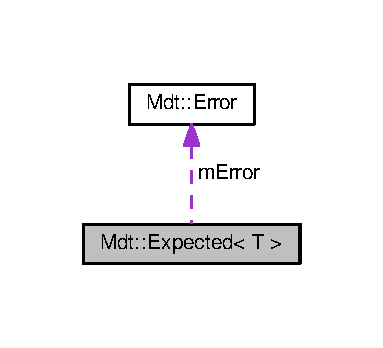
\includegraphics[width=184pt]{class_mdt_1_1_expected__coll__graph}
\end{center}
\end{figure}
\subsection*{Public Member Functions}
\begin{DoxyCompactItemize}
\item 
\hyperlink{class_mdt_1_1_expected_ab271cafc564b8dba7c5737a8e6f78a8d}{Expected} ()
\begin{DoxyCompactList}\small\item\em Construct a empty expected. \end{DoxyCompactList}\item 
\hyperlink{class_mdt_1_1_expected_a5046d26152b32d7184d756f00325cd60}{Expected} (const T \&v)
\begin{DoxyCompactList}\small\item\em Construct a expected with a value. \end{DoxyCompactList}\item 
\hyperlink{class_mdt_1_1_expected_abf1fd00a7d5508ab2030f729105de12f}{Expected} (T \&\&v)
\begin{DoxyCompactList}\small\item\em Construct a expected with a value. \end{DoxyCompactList}\item 
\hyperlink{class_mdt_1_1_expected_a98be29378d9ee4d855b041c5a347d967}{Expected} (const \hyperlink{class_mdt_1_1_error}{Mdt\+::\+Error} \&e)
\begin{DoxyCompactList}\small\item\em Construct a expected with a error. \end{DoxyCompactList}\item 
\hyperlink{class_mdt_1_1_expected_a63cf8d36dfb4657d39fcfb614f575ab4}{Expected} (\hyperlink{class_mdt_1_1_error}{Mdt\+::\+Error} \&\&e)
\begin{DoxyCompactList}\small\item\em Construct a expected with a error. \end{DoxyCompactList}\item 
\hyperlink{class_mdt_1_1_expected_a74ad44cec43f7cae5cd73388283818e3}{Expected} (const \hyperlink{class_mdt_1_1_expected}{Expected} \&other)
\begin{DoxyCompactList}\small\item\em Construct a copy of other. \end{DoxyCompactList}\item 
\hyperlink{class_mdt_1_1_expected_a8d14f0fbfb0c4e1acbfbae539f797aa8}{Expected} (\hyperlink{class_mdt_1_1_expected}{Expected} \&\&other)
\begin{DoxyCompactList}\small\item\em Construct by moving other. \end{DoxyCompactList}\item 
\hyperlink{class_mdt_1_1_expected_ab3694955007f559c7f394e9883aa44a0}{$\sim$\+Expected} ()
\begin{DoxyCompactList}\small\item\em Destructor. \end{DoxyCompactList}\item 
\hyperlink{class_mdt_1_1_expected}{Expected} \& \hyperlink{class_mdt_1_1_expected_a9c7eb862d4d49f2160a16e32ec302e6c}{operator=} (const T \&v)
\begin{DoxyCompactList}\small\item\em Assign a value. \end{DoxyCompactList}\item 
\hyperlink{class_mdt_1_1_expected}{Expected} \& \hyperlink{class_mdt_1_1_expected_a7c1272621b28c6750f4a230278d477da}{operator=} (T \&\&v)
\begin{DoxyCompactList}\small\item\em Assign a value. \end{DoxyCompactList}\item 
\hyperlink{class_mdt_1_1_expected}{Expected} \& \hyperlink{class_mdt_1_1_expected_a60b7b4811399f71568fda6731a7afd59}{operator=} (const \hyperlink{class_mdt_1_1_error}{Mdt\+::\+Error} \&e)
\begin{DoxyCompactList}\small\item\em Assign a error. \end{DoxyCompactList}\item 
\hyperlink{class_mdt_1_1_expected}{Expected} \& \hyperlink{class_mdt_1_1_expected_a97c105de76860ec6fa9ce7926d6bc6a4}{operator=} (\hyperlink{class_mdt_1_1_error}{Mdt\+::\+Error} \&\&e)
\begin{DoxyCompactList}\small\item\em Assign a error. \end{DoxyCompactList}\item 
\hyperlink{class_mdt_1_1_expected}{Expected} \& \hyperlink{class_mdt_1_1_expected_a95886cd2913a38e147186ed3d9e72a7c}{operator=} (const \hyperlink{class_mdt_1_1_expected}{Expected} \&other)
\begin{DoxyCompactList}\small\item\em Assign a \hyperlink{class_mdt_1_1_expected}{Expected}. \end{DoxyCompactList}\item 
\hyperlink{class_mdt_1_1_expected}{Expected} \& \hyperlink{class_mdt_1_1_expected_a2c8f56f9a45c4b9b70ae2c7eadb2b96d}{operator=} (\hyperlink{class_mdt_1_1_expected}{Expected} \&\&other)
\begin{DoxyCompactList}\small\item\em Assign a \hyperlink{class_mdt_1_1_expected}{Expected}. \end{DoxyCompactList}\item 
bool \hyperlink{class_mdt_1_1_expected_acddb65fce2a9823e36663cbca8eaadc5}{has\+Error} () const 
\begin{DoxyCompactList}\small\item\em Return true if a error was set. \end{DoxyCompactList}\item 
\hyperlink{class_mdt_1_1_error}{Mdt\+::\+Error} \& \hyperlink{class_mdt_1_1_expected_a4e144dbc496a80e289f32f845aefcf5c}{error} ()
\begin{DoxyCompactList}\small\item\em Access error. \end{DoxyCompactList}\item 
const \hyperlink{class_mdt_1_1_error}{Mdt\+::\+Error} \& \hyperlink{class_mdt_1_1_expected_aecfcbc42443c3a2267d8d7c49e6282e8}{error} () const 
\begin{DoxyCompactList}\small\item\em Access error (read only) \end{DoxyCompactList}\item 
bool \hyperlink{class_mdt_1_1_expected_a8e75fd1c7205ad0fedac14223312c09e}{has\+Value} () const 
\begin{DoxyCompactList}\small\item\em Return true if a value was set. \end{DoxyCompactList}\item 
\hyperlink{class_mdt_1_1_expected_aa88e1919edb8b192abab69bffadf660e}{operator bool} () const 
\begin{DoxyCompactList}\small\item\em Return true if a value was set. \end{DoxyCompactList}\item 
T \& \hyperlink{class_mdt_1_1_expected_a744546093eb011f8d3964d749a3cbea3}{value} ()
\begin{DoxyCompactList}\small\item\em Access value. \end{DoxyCompactList}\item 
const T \& \hyperlink{class_mdt_1_1_expected_a290f2b4456b100e7066a453ffe7e94e8}{value} () const 
\begin{DoxyCompactList}\small\item\em Access value (read only) \end{DoxyCompactList}\end{DoxyCompactItemize}


\subsection{Detailed Description}
\subsubsection*{template$<$typename T$>$\\*
class Mdt\+::\+Expected$<$ T $>$}

Contains a value or a error. 

\hyperlink{class_mdt_1_1_expected}{Expected} provides a basic support of expected value. This is inspired from A. Alexandrescu \textquotesingle{}s talk \char`\"{}\+Systematic Error Handling in C++\char`\"{} \+: \href{http://channel9.msdn.com/Shows/Going+Deep/C-and-Beyond-2012-Andrei-Alexandrescu-Systematic-Error-Handling-in-C}{\tt http\+://channel9.\+msdn.\+com/\+Shows/\+Going+\+Deep/\+C-\/and-\/\+Beyond-\/2012-\/\+Andrei-\/\+Alexandrescu-\/\+Systematic-\/\+Error-\/\+Handling-\/in-\/C}

\hyperlink{class_mdt_1_1_expected}{Mdt\+::\+Expected} is a very limited version of the concept. For more advanced and performant version, you should take a look at the official proposal\+: \href{https://github.com/viboes/std-make/tree/master/doc/proposal/expected}{\tt https\+://github.\+com/viboes/std-\/make/tree/master/doc/proposal/expected}


\begin{DoxyTemplParams}{Template Parameters}
{\em T} & Type of value \\
\hline
\end{DoxyTemplParams}


Definition at line 44 of file Expected.\+h.



\subsection{Constructor \& Destructor Documentation}
\index{Mdt\+::\+Expected@{Mdt\+::\+Expected}!Expected@{Expected}}
\index{Expected@{Expected}!Mdt\+::\+Expected@{Mdt\+::\+Expected}}
\subsubsection[{\texorpdfstring{Expected()}{Expected()}}]{\setlength{\rightskip}{0pt plus 5cm}template$<$typename T$>$ {\bf Mdt\+::\+Expected}$<$ T $>$\+::{\bf Expected} (
\begin{DoxyParamCaption}
{}
\end{DoxyParamCaption}
)\hspace{0.3cm}{\ttfamily [inline]}}\hypertarget{class_mdt_1_1_expected_ab271cafc564b8dba7c5737a8e6f78a8d}{}\label{class_mdt_1_1_expected_ab271cafc564b8dba7c5737a8e6f78a8d}


Construct a empty expected. 

A empty expected contains a null error (see \hyperlink{class_mdt_1_1_error_a2b6a7708216d0de056c7d9e7dc571e70}{Mdt\+::\+Error\+::is\+Null()}). 

Definition at line 53 of file Expected.\+h.

\index{Mdt\+::\+Expected@{Mdt\+::\+Expected}!Expected@{Expected}}
\index{Expected@{Expected}!Mdt\+::\+Expected@{Mdt\+::\+Expected}}
\subsubsection[{\texorpdfstring{Expected(const T \&v)}{Expected(const T &v)}}]{\setlength{\rightskip}{0pt plus 5cm}template$<$typename T$>$ {\bf Mdt\+::\+Expected}$<$ T $>$\+::{\bf Expected} (
\begin{DoxyParamCaption}
\item[{const T \&}]{v}
\end{DoxyParamCaption}
)\hspace{0.3cm}{\ttfamily [inline]}}\hypertarget{class_mdt_1_1_expected_a5046d26152b32d7184d756f00325cd60}{}\label{class_mdt_1_1_expected_a5046d26152b32d7184d756f00325cd60}


Construct a expected with a value. 



Definition at line 61 of file Expected.\+h.

\index{Mdt\+::\+Expected@{Mdt\+::\+Expected}!Expected@{Expected}}
\index{Expected@{Expected}!Mdt\+::\+Expected@{Mdt\+::\+Expected}}
\subsubsection[{\texorpdfstring{Expected(\+T \&\&v)}{Expected(T &&v)}}]{\setlength{\rightskip}{0pt plus 5cm}template$<$typename T$>$ {\bf Mdt\+::\+Expected}$<$ T $>$\+::{\bf Expected} (
\begin{DoxyParamCaption}
\item[{T \&\&}]{v}
\end{DoxyParamCaption}
)\hspace{0.3cm}{\ttfamily [inline]}}\hypertarget{class_mdt_1_1_expected_abf1fd00a7d5508ab2030f729105de12f}{}\label{class_mdt_1_1_expected_abf1fd00a7d5508ab2030f729105de12f}


Construct a expected with a value. 



Definition at line 69 of file Expected.\+h.

\index{Mdt\+::\+Expected@{Mdt\+::\+Expected}!Expected@{Expected}}
\index{Expected@{Expected}!Mdt\+::\+Expected@{Mdt\+::\+Expected}}
\subsubsection[{\texorpdfstring{Expected(const Mdt\+::\+Error \&e)}{Expected(const Mdt::Error &e)}}]{\setlength{\rightskip}{0pt plus 5cm}template$<$typename T$>$ {\bf Mdt\+::\+Expected}$<$ T $>$\+::{\bf Expected} (
\begin{DoxyParamCaption}
\item[{const {\bf Mdt\+::\+Error} \&}]{e}
\end{DoxyParamCaption}
)\hspace{0.3cm}{\ttfamily [inline]}}\hypertarget{class_mdt_1_1_expected_a98be29378d9ee4d855b041c5a347d967}{}\label{class_mdt_1_1_expected_a98be29378d9ee4d855b041c5a347d967}


Construct a expected with a error. 



Definition at line 77 of file Expected.\+h.

\index{Mdt\+::\+Expected@{Mdt\+::\+Expected}!Expected@{Expected}}
\index{Expected@{Expected}!Mdt\+::\+Expected@{Mdt\+::\+Expected}}
\subsubsection[{\texorpdfstring{Expected(\+Mdt\+::\+Error \&\&e)}{Expected(Mdt::Error &&e)}}]{\setlength{\rightskip}{0pt plus 5cm}template$<$typename T$>$ {\bf Mdt\+::\+Expected}$<$ T $>$\+::{\bf Expected} (
\begin{DoxyParamCaption}
\item[{{\bf Mdt\+::\+Error} \&\&}]{e}
\end{DoxyParamCaption}
)\hspace{0.3cm}{\ttfamily [inline]}}\hypertarget{class_mdt_1_1_expected_a63cf8d36dfb4657d39fcfb614f575ab4}{}\label{class_mdt_1_1_expected_a63cf8d36dfb4657d39fcfb614f575ab4}


Construct a expected with a error. 



Definition at line 85 of file Expected.\+h.

\index{Mdt\+::\+Expected@{Mdt\+::\+Expected}!Expected@{Expected}}
\index{Expected@{Expected}!Mdt\+::\+Expected@{Mdt\+::\+Expected}}
\subsubsection[{\texorpdfstring{Expected(const Expected \&other)}{Expected(const Expected &other)}}]{\setlength{\rightskip}{0pt plus 5cm}template$<$typename T$>$ {\bf Mdt\+::\+Expected}$<$ T $>$\+::{\bf Expected} (
\begin{DoxyParamCaption}
\item[{const {\bf Expected}$<$ T $>$ \&}]{other}
\end{DoxyParamCaption}
)\hspace{0.3cm}{\ttfamily [inline]}}\hypertarget{class_mdt_1_1_expected_a74ad44cec43f7cae5cd73388283818e3}{}\label{class_mdt_1_1_expected_a74ad44cec43f7cae5cd73388283818e3}


Construct a copy of other. 



Definition at line 93 of file Expected.\+h.

\index{Mdt\+::\+Expected@{Mdt\+::\+Expected}!Expected@{Expected}}
\index{Expected@{Expected}!Mdt\+::\+Expected@{Mdt\+::\+Expected}}
\subsubsection[{\texorpdfstring{Expected(\+Expected \&\&other)}{Expected(Expected &&other)}}]{\setlength{\rightskip}{0pt plus 5cm}template$<$typename T$>$ {\bf Mdt\+::\+Expected}$<$ T $>$\+::{\bf Expected} (
\begin{DoxyParamCaption}
\item[{{\bf Expected}$<$ T $>$ \&\&}]{other}
\end{DoxyParamCaption}
)\hspace{0.3cm}{\ttfamily [inline]}}\hypertarget{class_mdt_1_1_expected_a8d14f0fbfb0c4e1acbfbae539f797aa8}{}\label{class_mdt_1_1_expected_a8d14f0fbfb0c4e1acbfbae539f797aa8}


Construct by moving other. 



Definition at line 105 of file Expected.\+h.

\index{Mdt\+::\+Expected@{Mdt\+::\+Expected}!````~Expected@{$\sim$\+Expected}}
\index{````~Expected@{$\sim$\+Expected}!Mdt\+::\+Expected@{Mdt\+::\+Expected}}
\subsubsection[{\texorpdfstring{$\sim$\+Expected()}{~Expected()}}]{\setlength{\rightskip}{0pt plus 5cm}template$<$typename T$>$ {\bf Mdt\+::\+Expected}$<$ T $>$\+::$\sim${\bf Expected} (
\begin{DoxyParamCaption}
{}
\end{DoxyParamCaption}
)\hspace{0.3cm}{\ttfamily [inline]}}\hypertarget{class_mdt_1_1_expected_ab3694955007f559c7f394e9883aa44a0}{}\label{class_mdt_1_1_expected_ab3694955007f559c7f394e9883aa44a0}


Destructor. 



Definition at line 117 of file Expected.\+h.



\subsection{Member Function Documentation}
\index{Mdt\+::\+Expected@{Mdt\+::\+Expected}!error@{error}}
\index{error@{error}!Mdt\+::\+Expected@{Mdt\+::\+Expected}}
\subsubsection[{\texorpdfstring{error()}{error()}}]{\setlength{\rightskip}{0pt plus 5cm}template$<$typename T$>$ {\bf Mdt\+::\+Error}\& {\bf Mdt\+::\+Expected}$<$ T $>$\+::error (
\begin{DoxyParamCaption}
{}
\end{DoxyParamCaption}
)\hspace{0.3cm}{\ttfamily [inline]}}\hypertarget{class_mdt_1_1_expected_a4e144dbc496a80e289f32f845aefcf5c}{}\label{class_mdt_1_1_expected_a4e144dbc496a80e289f32f845aefcf5c}


Access error. 

\begin{DoxyPrecond}{Precondition}
this must contain a error 
\end{DoxyPrecond}


Definition at line 226 of file Expected.\+h.

\index{Mdt\+::\+Expected@{Mdt\+::\+Expected}!error@{error}}
\index{error@{error}!Mdt\+::\+Expected@{Mdt\+::\+Expected}}
\subsubsection[{\texorpdfstring{error() const }{error() const }}]{\setlength{\rightskip}{0pt plus 5cm}template$<$typename T$>$ const {\bf Mdt\+::\+Error}\& {\bf Mdt\+::\+Expected}$<$ T $>$\+::error (
\begin{DoxyParamCaption}
{}
\end{DoxyParamCaption}
) const\hspace{0.3cm}{\ttfamily [inline]}}\hypertarget{class_mdt_1_1_expected_aecfcbc42443c3a2267d8d7c49e6282e8}{}\label{class_mdt_1_1_expected_aecfcbc42443c3a2267d8d7c49e6282e8}


Access error (read only) 

\begin{DoxyPrecond}{Precondition}
this must contain a error 
\end{DoxyPrecond}


Definition at line 236 of file Expected.\+h.

\index{Mdt\+::\+Expected@{Mdt\+::\+Expected}!has\+Error@{has\+Error}}
\index{has\+Error@{has\+Error}!Mdt\+::\+Expected@{Mdt\+::\+Expected}}
\subsubsection[{\texorpdfstring{has\+Error() const }{hasError() const }}]{\setlength{\rightskip}{0pt plus 5cm}template$<$typename T$>$ bool {\bf Mdt\+::\+Expected}$<$ T $>$\+::has\+Error (
\begin{DoxyParamCaption}
{}
\end{DoxyParamCaption}
) const\hspace{0.3cm}{\ttfamily [inline]}}\hypertarget{class_mdt_1_1_expected_acddb65fce2a9823e36663cbca8eaadc5}{}\label{class_mdt_1_1_expected_acddb65fce2a9823e36663cbca8eaadc5}


Return true if a error was set. 



Definition at line 217 of file Expected.\+h.

\index{Mdt\+::\+Expected@{Mdt\+::\+Expected}!has\+Value@{has\+Value}}
\index{has\+Value@{has\+Value}!Mdt\+::\+Expected@{Mdt\+::\+Expected}}
\subsubsection[{\texorpdfstring{has\+Value() const }{hasValue() const }}]{\setlength{\rightskip}{0pt plus 5cm}template$<$typename T$>$ bool {\bf Mdt\+::\+Expected}$<$ T $>$\+::has\+Value (
\begin{DoxyParamCaption}
{}
\end{DoxyParamCaption}
) const\hspace{0.3cm}{\ttfamily [inline]}}\hypertarget{class_mdt_1_1_expected_a8e75fd1c7205ad0fedac14223312c09e}{}\label{class_mdt_1_1_expected_a8e75fd1c7205ad0fedac14223312c09e}


Return true if a value was set. 



Definition at line 244 of file Expected.\+h.

\index{Mdt\+::\+Expected@{Mdt\+::\+Expected}!operator bool@{operator bool}}
\index{operator bool@{operator bool}!Mdt\+::\+Expected@{Mdt\+::\+Expected}}
\subsubsection[{\texorpdfstring{operator bool() const }{operator bool() const }}]{\setlength{\rightskip}{0pt plus 5cm}template$<$typename T$>$ {\bf Mdt\+::\+Expected}$<$ T $>$\+::operator bool (
\begin{DoxyParamCaption}
{}
\end{DoxyParamCaption}
) const\hspace{0.3cm}{\ttfamily [inline]}}\hypertarget{class_mdt_1_1_expected_aa88e1919edb8b192abab69bffadf660e}{}\label{class_mdt_1_1_expected_aa88e1919edb8b192abab69bffadf660e}


Return true if a value was set. 



Definition at line 251 of file Expected.\+h.

\index{Mdt\+::\+Expected@{Mdt\+::\+Expected}!operator=@{operator=}}
\index{operator=@{operator=}!Mdt\+::\+Expected@{Mdt\+::\+Expected}}
\subsubsection[{\texorpdfstring{operator=(const T \&v)}{operator=(const T &v)}}]{\setlength{\rightskip}{0pt plus 5cm}template$<$typename T$>$ {\bf Expected}\& {\bf Mdt\+::\+Expected}$<$ T $>$\+::operator= (
\begin{DoxyParamCaption}
\item[{const T \&}]{v}
\end{DoxyParamCaption}
)\hspace{0.3cm}{\ttfamily [inline]}}\hypertarget{class_mdt_1_1_expected_a9c7eb862d4d49f2160a16e32ec302e6c}{}\label{class_mdt_1_1_expected_a9c7eb862d4d49f2160a16e32ec302e6c}


Assign a value. 



Definition at line 124 of file Expected.\+h.

\index{Mdt\+::\+Expected@{Mdt\+::\+Expected}!operator=@{operator=}}
\index{operator=@{operator=}!Mdt\+::\+Expected@{Mdt\+::\+Expected}}
\subsubsection[{\texorpdfstring{operator=(\+T \&\&v)}{operator=(T &&v)}}]{\setlength{\rightskip}{0pt plus 5cm}template$<$typename T$>$ {\bf Expected}\& {\bf Mdt\+::\+Expected}$<$ T $>$\+::operator= (
\begin{DoxyParamCaption}
\item[{T \&\&}]{v}
\end{DoxyParamCaption}
)\hspace{0.3cm}{\ttfamily [inline]}}\hypertarget{class_mdt_1_1_expected_a7c1272621b28c6750f4a230278d477da}{}\label{class_mdt_1_1_expected_a7c1272621b28c6750f4a230278d477da}


Assign a value. 



Definition at line 134 of file Expected.\+h.

\index{Mdt\+::\+Expected@{Mdt\+::\+Expected}!operator=@{operator=}}
\index{operator=@{operator=}!Mdt\+::\+Expected@{Mdt\+::\+Expected}}
\subsubsection[{\texorpdfstring{operator=(const Mdt\+::\+Error \&e)}{operator=(const Mdt::Error &e)}}]{\setlength{\rightskip}{0pt plus 5cm}template$<$typename T$>$ {\bf Expected}\& {\bf Mdt\+::\+Expected}$<$ T $>$\+::operator= (
\begin{DoxyParamCaption}
\item[{const {\bf Mdt\+::\+Error} \&}]{e}
\end{DoxyParamCaption}
)\hspace{0.3cm}{\ttfamily [inline]}}\hypertarget{class_mdt_1_1_expected_a60b7b4811399f71568fda6731a7afd59}{}\label{class_mdt_1_1_expected_a60b7b4811399f71568fda6731a7afd59}


Assign a error. 



Definition at line 144 of file Expected.\+h.

\index{Mdt\+::\+Expected@{Mdt\+::\+Expected}!operator=@{operator=}}
\index{operator=@{operator=}!Mdt\+::\+Expected@{Mdt\+::\+Expected}}
\subsubsection[{\texorpdfstring{operator=(\+Mdt\+::\+Error \&\&e)}{operator=(Mdt::Error &&e)}}]{\setlength{\rightskip}{0pt plus 5cm}template$<$typename T$>$ {\bf Expected}\& {\bf Mdt\+::\+Expected}$<$ T $>$\+::operator= (
\begin{DoxyParamCaption}
\item[{{\bf Mdt\+::\+Error} \&\&}]{e}
\end{DoxyParamCaption}
)\hspace{0.3cm}{\ttfamily [inline]}}\hypertarget{class_mdt_1_1_expected_a97c105de76860ec6fa9ce7926d6bc6a4}{}\label{class_mdt_1_1_expected_a97c105de76860ec6fa9ce7926d6bc6a4}


Assign a error. 



Definition at line 154 of file Expected.\+h.

\index{Mdt\+::\+Expected@{Mdt\+::\+Expected}!operator=@{operator=}}
\index{operator=@{operator=}!Mdt\+::\+Expected@{Mdt\+::\+Expected}}
\subsubsection[{\texorpdfstring{operator=(const Expected \&other)}{operator=(const Expected &other)}}]{\setlength{\rightskip}{0pt plus 5cm}template$<$typename T$>$ {\bf Expected}\& {\bf Mdt\+::\+Expected}$<$ T $>$\+::operator= (
\begin{DoxyParamCaption}
\item[{const {\bf Expected}$<$ T $>$ \&}]{other}
\end{DoxyParamCaption}
)\hspace{0.3cm}{\ttfamily [inline]}}\hypertarget{class_mdt_1_1_expected_a95886cd2913a38e147186ed3d9e72a7c}{}\label{class_mdt_1_1_expected_a95886cd2913a38e147186ed3d9e72a7c}


Assign a \hyperlink{class_mdt_1_1_expected}{Expected}. 



Definition at line 164 of file Expected.\+h.

\index{Mdt\+::\+Expected@{Mdt\+::\+Expected}!operator=@{operator=}}
\index{operator=@{operator=}!Mdt\+::\+Expected@{Mdt\+::\+Expected}}
\subsubsection[{\texorpdfstring{operator=(\+Expected \&\&other)}{operator=(Expected &&other)}}]{\setlength{\rightskip}{0pt plus 5cm}template$<$typename T$>$ {\bf Expected}\& {\bf Mdt\+::\+Expected}$<$ T $>$\+::operator= (
\begin{DoxyParamCaption}
\item[{{\bf Expected}$<$ T $>$ \&\&}]{other}
\end{DoxyParamCaption}
)\hspace{0.3cm}{\ttfamily [inline]}}\hypertarget{class_mdt_1_1_expected_a2c8f56f9a45c4b9b70ae2c7eadb2b96d}{}\label{class_mdt_1_1_expected_a2c8f56f9a45c4b9b70ae2c7eadb2b96d}


Assign a \hyperlink{class_mdt_1_1_expected}{Expected}. 



Definition at line 190 of file Expected.\+h.

\index{Mdt\+::\+Expected@{Mdt\+::\+Expected}!value@{value}}
\index{value@{value}!Mdt\+::\+Expected@{Mdt\+::\+Expected}}
\subsubsection[{\texorpdfstring{value()}{value()}}]{\setlength{\rightskip}{0pt plus 5cm}template$<$typename T$>$ T\& {\bf Mdt\+::\+Expected}$<$ T $>$\+::value (
\begin{DoxyParamCaption}
{}
\end{DoxyParamCaption}
)\hspace{0.3cm}{\ttfamily [inline]}}\hypertarget{class_mdt_1_1_expected_a744546093eb011f8d3964d749a3cbea3}{}\label{class_mdt_1_1_expected_a744546093eb011f8d3964d749a3cbea3}


Access value. 

\begin{DoxyPrecond}{Precondition}
this must contain a value 
\end{DoxyPrecond}


Definition at line 260 of file Expected.\+h.

\index{Mdt\+::\+Expected@{Mdt\+::\+Expected}!value@{value}}
\index{value@{value}!Mdt\+::\+Expected@{Mdt\+::\+Expected}}
\subsubsection[{\texorpdfstring{value() const }{value() const }}]{\setlength{\rightskip}{0pt plus 5cm}template$<$typename T$>$ const T\& {\bf Mdt\+::\+Expected}$<$ T $>$\+::value (
\begin{DoxyParamCaption}
{}
\end{DoxyParamCaption}
) const\hspace{0.3cm}{\ttfamily [inline]}}\hypertarget{class_mdt_1_1_expected_a290f2b4456b100e7066a453ffe7e94e8}{}\label{class_mdt_1_1_expected_a290f2b4456b100e7066a453ffe7e94e8}


Access value (read only) 

\begin{DoxyPrecond}{Precondition}
this must contain a value 
\end{DoxyPrecond}


Definition at line 270 of file Expected.\+h.



The documentation for this class was generated from the following file\+:\begin{DoxyCompactItemize}
\item 
libs/\+Expected/src/\+Mdt/Expected.\+h\end{DoxyCompactItemize}

\hypertarget{class_mdt_1_1_error_logger_1_1_file_backend}{}\section{Mdt\+:\+:Error\+Logger\+:\+:File\+Backend Class Reference}
\label{class_mdt_1_1_error_logger_1_1_file_backend}\index{Mdt\+::\+Error\+Logger\+::\+File\+Backend@{Mdt\+::\+Error\+Logger\+::\+File\+Backend}}


File backend for error \hyperlink{class_mdt_1_1_error_logger_1_1_logger}{Logger}.  




{\ttfamily \#include $<$File\+Backend.\+h$>$}



Inheritance diagram for Mdt\+:\+:Error\+Logger\+:\+:File\+Backend\+:\nopagebreak
\begin{figure}[H]
\begin{center}
\leavevmode
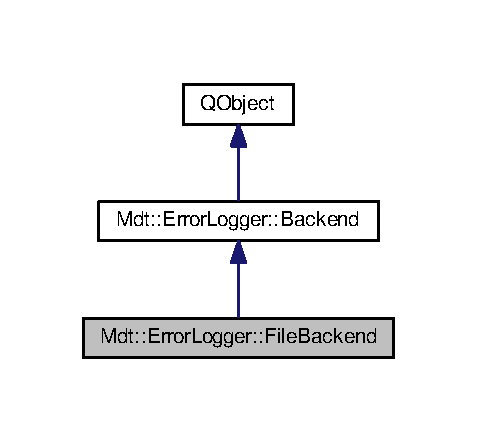
\includegraphics[width=229pt]{class_mdt_1_1_error_logger_1_1_file_backend__inherit__graph}
\end{center}
\end{figure}


Collaboration diagram for Mdt\+:\+:Error\+Logger\+:\+:File\+Backend\+:\nopagebreak
\begin{figure}[H]
\begin{center}
\leavevmode
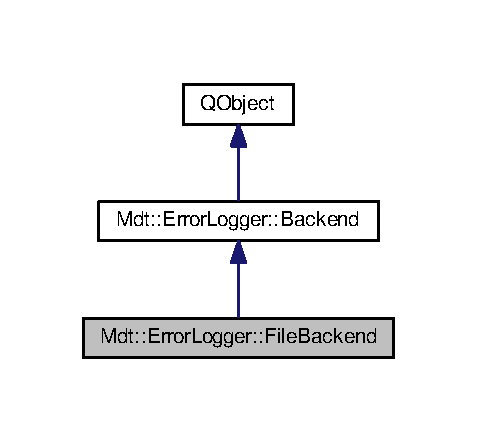
\includegraphics[width=229pt]{class_mdt_1_1_error_logger_1_1_file_backend__coll__graph}
\end{center}
\end{figure}
\subsection*{Public Member Functions}
\begin{DoxyCompactItemize}
\item 
\hyperlink{class_mdt_1_1_error_logger_1_1_file_backend_a8587ac2a6cd89416878b389138e79a3a}{File\+Backend} ()
\begin{DoxyCompactList}\small\item\em Constructor. \end{DoxyCompactList}\item 
\hyperlink{class_mdt_1_1_error_logger_1_1_file_backend_a5f7262e481d756d7145bbfa42aeca91e}{$\sim$\+File\+Backend} ()
\begin{DoxyCompactList}\small\item\em Destructor. \end{DoxyCompactList}\item 
bool \hyperlink{class_mdt_1_1_error_logger_1_1_file_backend_a844fc6f89a147b0713700028808e364a}{set\+Log\+File\+Path} (const Q\+String \&path, qint64 \hyperlink{class_mdt_1_1_error_logger_1_1_file_backend_a8c5943cdd59ed5941c72490d7b414359}{max\+File\+Size}=1024 $\ast$1024)
\begin{DoxyCompactList}\small\item\em Set path to log file. \end{DoxyCompactList}\item 
Q\+String \hyperlink{class_mdt_1_1_error_logger_1_1_file_backend_ac25cd41dbbe940bf0247e5054ce8805e}{log\+File\+Path} () const 
\begin{DoxyCompactList}\small\item\em Get log file path. \end{DoxyCompactList}\item 
Q\+String \hyperlink{class_mdt_1_1_error_logger_1_1_file_backend_a7c79c940be2f03f22111638d2e749a64}{backup\+Log\+File\+Path} () const 
\begin{DoxyCompactList}\small\item\em Get backup log file path. \end{DoxyCompactList}\item 
qint64 \hyperlink{class_mdt_1_1_error_logger_1_1_file_backend_a8c5943cdd59ed5941c72490d7b414359}{max\+File\+Size} () const 
\begin{DoxyCompactList}\small\item\em Get maximum log file size. \end{DoxyCompactList}\item 
void \hyperlink{class_mdt_1_1_error_logger_1_1_file_backend_a31b8314d523a491b5441276122daed87}{log\+Error} (const \hyperlink{class_mdt_1_1_error}{Error} \&error)
\begin{DoxyCompactList}\small\item\em Log given error. \end{DoxyCompactList}\end{DoxyCompactItemize}
\subsection*{Additional Inherited Members}


\subsection{Detailed Description}
File backend for error \hyperlink{class_mdt_1_1_error_logger_1_1_logger}{Logger}. 

Definition at line 34 of file File\+Backend.\+h.



\subsection{Constructor \& Destructor Documentation}
\index{Mdt\+::\+Error\+Logger\+::\+File\+Backend@{Mdt\+::\+Error\+Logger\+::\+File\+Backend}!File\+Backend@{File\+Backend}}
\index{File\+Backend@{File\+Backend}!Mdt\+::\+Error\+Logger\+::\+File\+Backend@{Mdt\+::\+Error\+Logger\+::\+File\+Backend}}
\subsubsection[{\texorpdfstring{File\+Backend()}{FileBackend()}}]{\setlength{\rightskip}{0pt plus 5cm}Mdt\+::\+Error\+Logger\+::\+File\+Backend\+::\+File\+Backend (
\begin{DoxyParamCaption}
{}
\end{DoxyParamCaption}
)}\hypertarget{class_mdt_1_1_error_logger_1_1_file_backend_a8587ac2a6cd89416878b389138e79a3a}{}\label{class_mdt_1_1_error_logger_1_1_file_backend_a8587ac2a6cd89416878b389138e79a3a}


Constructor. 



Definition at line 32 of file File\+Backend.\+cpp.

\index{Mdt\+::\+Error\+Logger\+::\+File\+Backend@{Mdt\+::\+Error\+Logger\+::\+File\+Backend}!````~File\+Backend@{$\sim$\+File\+Backend}}
\index{````~File\+Backend@{$\sim$\+File\+Backend}!Mdt\+::\+Error\+Logger\+::\+File\+Backend@{Mdt\+::\+Error\+Logger\+::\+File\+Backend}}
\subsubsection[{\texorpdfstring{$\sim$\+File\+Backend()}{~FileBackend()}}]{\setlength{\rightskip}{0pt plus 5cm}Mdt\+::\+Error\+Logger\+::\+File\+Backend\+::$\sim$\+File\+Backend (
\begin{DoxyParamCaption}
{}
\end{DoxyParamCaption}
)}\hypertarget{class_mdt_1_1_error_logger_1_1_file_backend_a5f7262e481d756d7145bbfa42aeca91e}{}\label{class_mdt_1_1_error_logger_1_1_file_backend_a5f7262e481d756d7145bbfa42aeca91e}


Destructor. 



Definition at line 37 of file File\+Backend.\+cpp.



\subsection{Member Function Documentation}
\index{Mdt\+::\+Error\+Logger\+::\+File\+Backend@{Mdt\+::\+Error\+Logger\+::\+File\+Backend}!backup\+Log\+File\+Path@{backup\+Log\+File\+Path}}
\index{backup\+Log\+File\+Path@{backup\+Log\+File\+Path}!Mdt\+::\+Error\+Logger\+::\+File\+Backend@{Mdt\+::\+Error\+Logger\+::\+File\+Backend}}
\subsubsection[{\texorpdfstring{backup\+Log\+File\+Path() const }{backupLogFilePath() const }}]{\setlength{\rightskip}{0pt plus 5cm}Q\+String Mdt\+::\+Error\+Logger\+::\+File\+Backend\+::backup\+Log\+File\+Path (
\begin{DoxyParamCaption}
{}
\end{DoxyParamCaption}
) const}\hypertarget{class_mdt_1_1_error_logger_1_1_file_backend_a7c79c940be2f03f22111638d2e749a64}{}\label{class_mdt_1_1_error_logger_1_1_file_backend_a7c79c940be2f03f22111638d2e749a64}


Get backup log file path. 



Definition at line 64 of file File\+Backend.\+cpp.

\index{Mdt\+::\+Error\+Logger\+::\+File\+Backend@{Mdt\+::\+Error\+Logger\+::\+File\+Backend}!log\+Error@{log\+Error}}
\index{log\+Error@{log\+Error}!Mdt\+::\+Error\+Logger\+::\+File\+Backend@{Mdt\+::\+Error\+Logger\+::\+File\+Backend}}
\subsubsection[{\texorpdfstring{log\+Error(const Error \&error)}{logError(const Error &error)}}]{\setlength{\rightskip}{0pt plus 5cm}void Mdt\+::\+Error\+Logger\+::\+File\+Backend\+::log\+Error (
\begin{DoxyParamCaption}
\item[{const {\bf Error} \&}]{error}
\end{DoxyParamCaption}
)\hspace{0.3cm}{\ttfamily [virtual]}}\hypertarget{class_mdt_1_1_error_logger_1_1_file_backend_a31b8314d523a491b5441276122daed87}{}\label{class_mdt_1_1_error_logger_1_1_file_backend_a31b8314d523a491b5441276122daed87}


Log given error. 



Implements \hyperlink{class_mdt_1_1_error_logger_1_1_backend_acf37cfc576269934ca8ce04e3601058d}{Mdt\+::\+Error\+Logger\+::\+Backend}.



Definition at line 74 of file File\+Backend.\+cpp.

\index{Mdt\+::\+Error\+Logger\+::\+File\+Backend@{Mdt\+::\+Error\+Logger\+::\+File\+Backend}!log\+File\+Path@{log\+File\+Path}}
\index{log\+File\+Path@{log\+File\+Path}!Mdt\+::\+Error\+Logger\+::\+File\+Backend@{Mdt\+::\+Error\+Logger\+::\+File\+Backend}}
\subsubsection[{\texorpdfstring{log\+File\+Path() const }{logFilePath() const }}]{\setlength{\rightskip}{0pt plus 5cm}Q\+String Mdt\+::\+Error\+Logger\+::\+File\+Backend\+::log\+File\+Path (
\begin{DoxyParamCaption}
{}
\end{DoxyParamCaption}
) const}\hypertarget{class_mdt_1_1_error_logger_1_1_file_backend_ac25cd41dbbe940bf0247e5054ce8805e}{}\label{class_mdt_1_1_error_logger_1_1_file_backend_ac25cd41dbbe940bf0247e5054ce8805e}


Get log file path. 



Definition at line 59 of file File\+Backend.\+cpp.

\index{Mdt\+::\+Error\+Logger\+::\+File\+Backend@{Mdt\+::\+Error\+Logger\+::\+File\+Backend}!max\+File\+Size@{max\+File\+Size}}
\index{max\+File\+Size@{max\+File\+Size}!Mdt\+::\+Error\+Logger\+::\+File\+Backend@{Mdt\+::\+Error\+Logger\+::\+File\+Backend}}
\subsubsection[{\texorpdfstring{max\+File\+Size() const }{maxFileSize() const }}]{\setlength{\rightskip}{0pt plus 5cm}qint64 Mdt\+::\+Error\+Logger\+::\+File\+Backend\+::max\+File\+Size (
\begin{DoxyParamCaption}
{}
\end{DoxyParamCaption}
) const}\hypertarget{class_mdt_1_1_error_logger_1_1_file_backend_a8c5943cdd59ed5941c72490d7b414359}{}\label{class_mdt_1_1_error_logger_1_1_file_backend_a8c5943cdd59ed5941c72490d7b414359}


Get maximum log file size. 



Definition at line 69 of file File\+Backend.\+cpp.

\index{Mdt\+::\+Error\+Logger\+::\+File\+Backend@{Mdt\+::\+Error\+Logger\+::\+File\+Backend}!set\+Log\+File\+Path@{set\+Log\+File\+Path}}
\index{set\+Log\+File\+Path@{set\+Log\+File\+Path}!Mdt\+::\+Error\+Logger\+::\+File\+Backend@{Mdt\+::\+Error\+Logger\+::\+File\+Backend}}
\subsubsection[{\texorpdfstring{set\+Log\+File\+Path(const Q\+String \&path, qint64 max\+File\+Size=1024 $\ast$1024)}{setLogFilePath(const QString &path, qint64 maxFileSize=1024 *1024)}}]{\setlength{\rightskip}{0pt plus 5cm}bool Mdt\+::\+Error\+Logger\+::\+File\+Backend\+::set\+Log\+File\+Path (
\begin{DoxyParamCaption}
\item[{const Q\+String \&}]{path, }
\item[{qint64}]{max\+File\+Size = {\ttfamily 1024$\ast$1024}}
\end{DoxyParamCaption}
)}\hypertarget{class_mdt_1_1_error_logger_1_1_file_backend_a844fc6f89a147b0713700028808e364a}{}\label{class_mdt_1_1_error_logger_1_1_file_backend_a844fc6f89a147b0713700028808e364a}


Set path to log file. 


\begin{DoxyParams}{Parameters}
{\em path} & Path to the log file. Note that a backup is made in same directory than file given by path, with a other exention. \\
\hline
{\em max\+File\+Size} & Maximum size allowed for log file \mbox{[}Byte\mbox{]} Also note that the file can be some bytes greater than specified size. \\
\hline
\end{DoxyParams}
\begin{DoxyNote}{Note}
This function should only be called before this Logger\+File\+Backend is passed to the \hyperlink{class_mdt_1_1_error_logger_1_1_logger}{Logger} (changing file path while \hyperlink{class_mdt_1_1_error_logger_1_1_logger}{Logger} is calling \hyperlink{class_mdt_1_1_error_logger_1_1_file_backend_a31b8314d523a491b5441276122daed87}{log\+Error()} is undefined behaviour). 
\end{DoxyNote}


Definition at line 41 of file File\+Backend.\+cpp.



The documentation for this class was generated from the following files\+:\begin{DoxyCompactItemize}
\item 
libs/\+Error\+\_\+\+Core/src/\+Mdt/\+Error\+Logger/File\+Backend.\+h\item 
libs/\+Error\+\_\+\+Core/src/\+Mdt/\+Error\+Logger/File\+Backend.\+cpp\end{DoxyCompactItemize}

\hypertarget{class_mdt_1_1_deploy_utils_1_1_file_copier}{}\section{Mdt\+:\+:Deploy\+Utils\+:\+:File\+Copier Class Reference}
\label{class_mdt_1_1_deploy_utils_1_1_file_copier}\index{Mdt\+::\+Deploy\+Utils\+::\+File\+Copier@{Mdt\+::\+Deploy\+Utils\+::\+File\+Copier}}


Provides utilities for files and directories manipulation.  




{\ttfamily \#include $<$File\+Copier.\+h$>$}



Inheritance diagram for Mdt\+:\+:Deploy\+Utils\+:\+:File\+Copier\+:
\nopagebreak
\begin{figure}[H]
\begin{center}
\leavevmode
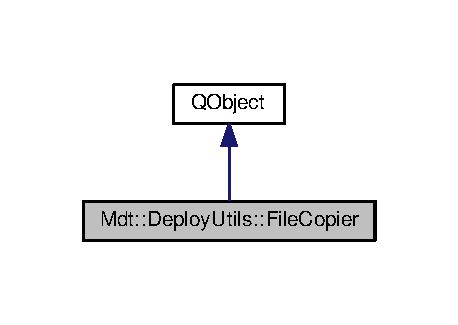
\includegraphics[width=220pt]{class_mdt_1_1_deploy_utils_1_1_file_copier__inherit__graph}
\end{center}
\end{figure}


Collaboration diagram for Mdt\+:\+:Deploy\+Utils\+:\+:File\+Copier\+:
\nopagebreak
\begin{figure}[H]
\begin{center}
\leavevmode
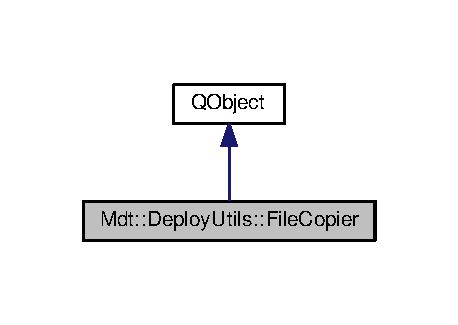
\includegraphics[width=220pt]{class_mdt_1_1_deploy_utils_1_1_file_copier__coll__graph}
\end{center}
\end{figure}
\subsection*{Public Member Functions}
\begin{DoxyCompactItemize}
\item 
\hyperlink{class_mdt_1_1_deploy_utils_1_1_file_copier_af21c6f7e6fc3074e2fed28d127b29edf}{File\+Copier} (\hyperlink{class_q_object}{Q\+Object} $\ast$parent=nullptr)
\begin{DoxyCompactList}\small\item\em Constructor. \end{DoxyCompactList}\item 
bool \hyperlink{class_mdt_1_1_deploy_utils_1_1_file_copier_ab1040ccbe34149841a42191e7ced3ba4}{create\+Directory} (const Q\+String \&directory\+Path)
\begin{DoxyCompactList}\small\item\em Create a directory. \end{DoxyCompactList}\item 
bool \hyperlink{class_mdt_1_1_deploy_utils_1_1_file_copier_ab81974d2e6e5b2260a8147c3400dcb3a}{copy\+Libraries} (const \hyperlink{class_mdt_1_1_deploy_utils_1_1_library_info_list}{Library\+Info\+List} \&libraries, const Q\+String \&destination\+Directory\+Path)
\begin{DoxyCompactList}\small\item\em Copy a list of libraries to a directory. \end{DoxyCompactList}\item 
\hyperlink{class_mdt_1_1_error}{Mdt\+::\+Error} \hyperlink{class_mdt_1_1_deploy_utils_1_1_file_copier_a8e82df0b666b0cdb45edd878af31893f}{last\+Error} () const 
\begin{DoxyCompactList}\small\item\em Get last error. \end{DoxyCompactList}\end{DoxyCompactItemize}


\subsection{Detailed Description}
Provides utilities for files and directories manipulation. 

Definition at line 34 of file File\+Copier.\+h.



\subsection{Constructor \& Destructor Documentation}
\index{Mdt\+::\+Deploy\+Utils\+::\+File\+Copier@{Mdt\+::\+Deploy\+Utils\+::\+File\+Copier}!File\+Copier@{File\+Copier}}
\index{File\+Copier@{File\+Copier}!Mdt\+::\+Deploy\+Utils\+::\+File\+Copier@{Mdt\+::\+Deploy\+Utils\+::\+File\+Copier}}
\subsubsection[{\texorpdfstring{File\+Copier(\+Q\+Object $\ast$parent=nullptr)}{FileCopier(QObject *parent=nullptr)}}]{\setlength{\rightskip}{0pt plus 5cm}Mdt\+::\+Deploy\+Utils\+::\+File\+Copier\+::\+File\+Copier (
\begin{DoxyParamCaption}
\item[{{\bf Q\+Object} $\ast$}]{parent = {\ttfamily nullptr}}
\end{DoxyParamCaption}
)\hspace{0.3cm}{\ttfamily [explicit]}}\hypertarget{class_mdt_1_1_deploy_utils_1_1_file_copier_af21c6f7e6fc3074e2fed28d127b29edf}{}\label{class_mdt_1_1_deploy_utils_1_1_file_copier_af21c6f7e6fc3074e2fed28d127b29edf}


Constructor. 



Definition at line 33 of file File\+Copier.\+cpp.



\subsection{Member Function Documentation}
\index{Mdt\+::\+Deploy\+Utils\+::\+File\+Copier@{Mdt\+::\+Deploy\+Utils\+::\+File\+Copier}!copy\+Libraries@{copy\+Libraries}}
\index{copy\+Libraries@{copy\+Libraries}!Mdt\+::\+Deploy\+Utils\+::\+File\+Copier@{Mdt\+::\+Deploy\+Utils\+::\+File\+Copier}}
\subsubsection[{\texorpdfstring{copy\+Libraries(const Library\+Info\+List \&libraries, const Q\+String \&destination\+Directory\+Path)}{copyLibraries(const LibraryInfoList &libraries, const QString &destinationDirectoryPath)}}]{\setlength{\rightskip}{0pt plus 5cm}bool Mdt\+::\+Deploy\+Utils\+::\+File\+Copier\+::copy\+Libraries (
\begin{DoxyParamCaption}
\item[{const {\bf Library\+Info\+List} \&}]{libraries, }
\item[{const Q\+String \&}]{destination\+Directory\+Path}
\end{DoxyParamCaption}
)}\hypertarget{class_mdt_1_1_deploy_utils_1_1_file_copier_ab81974d2e6e5b2260a8147c3400dcb3a}{}\label{class_mdt_1_1_deploy_utils_1_1_file_copier_ab81974d2e6e5b2260a8147c3400dcb3a}


Copy a list of libraries to a directory. 

If directory designed by {\itshape destination\+Directory\+Path} does not exist, it will first be created using \hyperlink{class_mdt_1_1_deploy_utils_1_1_file_copier_ab1040ccbe34149841a42191e7ced3ba4}{create\+Directory()}. 

Definition at line 63 of file File\+Copier.\+cpp.

\index{Mdt\+::\+Deploy\+Utils\+::\+File\+Copier@{Mdt\+::\+Deploy\+Utils\+::\+File\+Copier}!create\+Directory@{create\+Directory}}
\index{create\+Directory@{create\+Directory}!Mdt\+::\+Deploy\+Utils\+::\+File\+Copier@{Mdt\+::\+Deploy\+Utils\+::\+File\+Copier}}
\subsubsection[{\texorpdfstring{create\+Directory(const Q\+String \&directory\+Path)}{createDirectory(const QString &directoryPath)}}]{\setlength{\rightskip}{0pt plus 5cm}bool Mdt\+::\+Deploy\+Utils\+::\+File\+Copier\+::create\+Directory (
\begin{DoxyParamCaption}
\item[{const Q\+String \&}]{directory\+Path}
\end{DoxyParamCaption}
)}\hypertarget{class_mdt_1_1_deploy_utils_1_1_file_copier_ab1040ccbe34149841a42191e7ced3ba4}{}\label{class_mdt_1_1_deploy_utils_1_1_file_copier_ab1040ccbe34149841a42191e7ced3ba4}


Create a directory. 

Will create a directory designed by {\itshape directory\+Path} if it not allready exists. If parent directories are missing, they will also be created. 

Definition at line 38 of file File\+Copier.\+cpp.

\index{Mdt\+::\+Deploy\+Utils\+::\+File\+Copier@{Mdt\+::\+Deploy\+Utils\+::\+File\+Copier}!last\+Error@{last\+Error}}
\index{last\+Error@{last\+Error}!Mdt\+::\+Deploy\+Utils\+::\+File\+Copier@{Mdt\+::\+Deploy\+Utils\+::\+File\+Copier}}
\subsubsection[{\texorpdfstring{last\+Error() const }{lastError() const }}]{\setlength{\rightskip}{0pt plus 5cm}{\bf Mdt\+::\+Error} Mdt\+::\+Deploy\+Utils\+::\+File\+Copier\+::last\+Error (
\begin{DoxyParamCaption}
{}
\end{DoxyParamCaption}
) const\hspace{0.3cm}{\ttfamily [inline]}}\hypertarget{class_mdt_1_1_deploy_utils_1_1_file_copier_a8e82df0b666b0cdb45edd878af31893f}{}\label{class_mdt_1_1_deploy_utils_1_1_file_copier_a8e82df0b666b0cdb45edd878af31893f}


Get last error. 



Definition at line 62 of file File\+Copier.\+h.



The documentation for this class was generated from the following files\+:\begin{DoxyCompactItemize}
\item 
libs/\+Deploy\+Utils\+\_\+\+Core/src/\+Mdt/\+Deploy\+Utils/File\+Copier.\+h\item 
libs/\+Deploy\+Utils\+\_\+\+Core/src/\+Mdt/\+Deploy\+Utils/File\+Copier.\+cpp\end{DoxyCompactItemize}

\hypertarget{struct_mdt_1_1_plain_text_1_1_file_input_iterator}{}\section{Mdt\+:\+:Plain\+Text\+:\+:File\+Input\+Iterator Struct Reference}
\label{struct_mdt_1_1_plain_text_1_1_file_input_iterator}\index{Mdt\+::\+Plain\+Text\+::\+File\+Input\+Iterator@{Mdt\+::\+Plain\+Text\+::\+File\+Input\+Iterator}}


Iterator that acts on a I/O device.  




{\ttfamily \#include $<$File\+Input\+Iterator.\+h$>$}

\subsection*{Public Member Functions}
\begin{DoxyCompactItemize}
\item 
\hyperlink{struct_mdt_1_1_plain_text_1_1_file_input_iterator_a53ed659924fc406bd89c6c6f04018159}{File\+Input\+Iterator} ()
\begin{DoxyCompactList}\small\item\em Constructs a end-\/of-\/stream iterator. \end{DoxyCompactList}\item 
\hyperlink{struct_mdt_1_1_plain_text_1_1_file_input_iterator_ad34d8fff6203f66a4e78283c30079a8f}{File\+Input\+Iterator} (Q\+I\+O\+Device $\ast$device, const Q\+Byte\+Array \&encoding)
\begin{DoxyCompactList}\small\item\em Construct a iterator that acts on device. \end{DoxyCompactList}\item 
\hyperlink{struct_mdt_1_1_plain_text_1_1_file_input_iterator_a7cba55a1d994d46dcddd36dcbf79381b}{File\+Input\+Iterator} (const \hyperlink{struct_mdt_1_1_plain_text_1_1_file_input_iterator}{File\+Input\+Iterator} \&other)=default
\begin{DoxyCompactList}\small\item\em Copy on base of other iterator. \end{DoxyCompactList}\item 
\hyperlink{struct_mdt_1_1_plain_text_1_1_file_input_iterator_aa3921f03022ead216ef23e27aae1ea69}{File\+Input\+Iterator} (\hyperlink{struct_mdt_1_1_plain_text_1_1_file_input_iterator}{File\+Input\+Iterator} \&\&other)=default
\begin{DoxyCompactList}\small\item\em Move constructor. \end{DoxyCompactList}\item 
\hyperlink{struct_mdt_1_1_plain_text_1_1_file_input_iterator}{File\+Input\+Iterator} \& \hyperlink{struct_mdt_1_1_plain_text_1_1_file_input_iterator_adc29c4e6d155d676ca78d1f5ab8032f0}{operator=} (const \hyperlink{struct_mdt_1_1_plain_text_1_1_file_input_iterator}{File\+Input\+Iterator} \&other)=default
\begin{DoxyCompactList}\small\item\em Assign other iterator. \end{DoxyCompactList}\item 
bool \hyperlink{struct_mdt_1_1_plain_text_1_1_file_input_iterator_a5c8774871108780cc0c746a2b37163c5}{set\+Source} (Q\+I\+O\+Device $\ast$device, const Q\+Byte\+Array \&encoding)
\begin{DoxyCompactList}\small\item\em Set source. \end{DoxyCompactList}\item 
void \hyperlink{struct_mdt_1_1_plain_text_1_1_file_input_iterator_a4197ea452aa5e75602d1a38e08baef81}{clear} ()
\begin{DoxyCompactList}\small\item\em Clear. \end{DoxyCompactList}\item 
\hyperlink{struct_mdt_1_1_plain_text_1_1_file_input_iterator}{File\+Input\+Iterator} \& \hyperlink{struct_mdt_1_1_plain_text_1_1_file_input_iterator_a0048b29d504d922ab979c22063eae21a}{operator++} ()
\begin{DoxyCompactList}\small\item\em Increment iterator (pre-\/increment) \end{DoxyCompactList}\item 
\hyperlink{struct_mdt_1_1_plain_text_1_1_file_input_iterator}{File\+Input\+Iterator} \hyperlink{struct_mdt_1_1_plain_text_1_1_file_input_iterator_a28f4e511a266f8ffcd2a5844127050d7}{operator++} (int)
\begin{DoxyCompactList}\small\item\em Increment iterator (post-\/increment) \end{DoxyCompactList}\item 
reference \hyperlink{struct_mdt_1_1_plain_text_1_1_file_input_iterator_a5c3f8149a81d8f6f059fffe188f4110b}{operator$\ast$} ()
\begin{DoxyCompactList}\small\item\em Get last read value. \end{DoxyCompactList}\item 
bool \hyperlink{struct_mdt_1_1_plain_text_1_1_file_input_iterator_a5461a2af93730a77642d56333f952704}{is\+Eof} () const 
\begin{DoxyCompactList}\small\item\em Check if this iterator is a end-\/of-\/stream iterator. \end{DoxyCompactList}\item 
bool \hyperlink{struct_mdt_1_1_plain_text_1_1_file_input_iterator_afa93baaf36f16456fa29451fa4fcf9f3}{error\+Occured} () const 
\begin{DoxyCompactList}\small\item\em Check if a error occured. \end{DoxyCompactList}\item 
\hyperlink{class_mdt_1_1_error}{Mdt\+::\+Error} \hyperlink{struct_mdt_1_1_plain_text_1_1_file_input_iterator_a0d9ed2faf04b16e3a03fabd6a09db67e}{last\+Error} () const 
\begin{DoxyCompactList}\small\item\em Get last error. \end{DoxyCompactList}\end{DoxyCompactItemize}
\subsection*{Friends}
\begin{DoxyCompactItemize}
\item 
bool \hyperlink{struct_mdt_1_1_plain_text_1_1_file_input_iterator_a0728389e31ef4f52e51a7725f31cdf52}{operator==} (const \hyperlink{struct_mdt_1_1_plain_text_1_1_file_input_iterator}{File\+Input\+Iterator} \&a, const \hyperlink{struct_mdt_1_1_plain_text_1_1_file_input_iterator}{File\+Input\+Iterator} \&b)
\begin{DoxyCompactList}\small\item\em Returns true if a and b are E\+OF iterators, or a and b are valid iterators. \end{DoxyCompactList}\item 
bool \hyperlink{struct_mdt_1_1_plain_text_1_1_file_input_iterator_a72b46be4d1041d39fd539fda1124eb45}{operator!=} (const \hyperlink{struct_mdt_1_1_plain_text_1_1_file_input_iterator}{File\+Input\+Iterator} \&a, const \hyperlink{struct_mdt_1_1_plain_text_1_1_file_input_iterator}{File\+Input\+Iterator} \&b)
\begin{DoxyCompactList}\small\item\em See \hyperlink{struct_mdt_1_1_plain_text_1_1_file_input_iterator_a0728389e31ef4f52e51a7725f31cdf52}{operator==()} \end{DoxyCompactList}\end{DoxyCompactItemize}


\subsection{Detailed Description}
Iterator that acts on a I/O device. 

This iterator can be used by with Boost Spirit multipass\+\_\+iterator.

\hyperlink{struct_mdt_1_1_plain_text_1_1_file_input_iterator}{File\+Input\+Iterator} is a single-\/pass input iterator that reads data from a Q\+I\+O\+Device. When the iterator is incremented, it will take a char from its internal buffer, witch is handled by \hyperlink{class_mdt_1_1_plain_text_1_1_file_input_iterator_shared_data}{File\+Input\+Iterator\+Shared\+Data}. When no data is available anymore in the buffer, a chunck of data is read from Q\+I\+O\+Device and decoded to unicode. 

Definition at line 47 of file File\+Input\+Iterator.\+h.



\subsection{Constructor \& Destructor Documentation}
\index{Mdt\+::\+Plain\+Text\+::\+File\+Input\+Iterator@{Mdt\+::\+Plain\+Text\+::\+File\+Input\+Iterator}!File\+Input\+Iterator@{File\+Input\+Iterator}}
\index{File\+Input\+Iterator@{File\+Input\+Iterator}!Mdt\+::\+Plain\+Text\+::\+File\+Input\+Iterator@{Mdt\+::\+Plain\+Text\+::\+File\+Input\+Iterator}}
\subsubsection[{\texorpdfstring{File\+Input\+Iterator()}{FileInputIterator()}}]{\setlength{\rightskip}{0pt plus 5cm}Mdt\+::\+Plain\+Text\+::\+File\+Input\+Iterator\+::\+File\+Input\+Iterator (
\begin{DoxyParamCaption}
{}
\end{DoxyParamCaption}
)\hspace{0.3cm}{\ttfamily [inline]}}\hypertarget{struct_mdt_1_1_plain_text_1_1_file_input_iterator_a53ed659924fc406bd89c6c6f04018159}{}\label{struct_mdt_1_1_plain_text_1_1_file_input_iterator_a53ed659924fc406bd89c6c6f04018159}


Constructs a end-\/of-\/stream iterator. 



Definition at line 59 of file File\+Input\+Iterator.\+h.

\index{Mdt\+::\+Plain\+Text\+::\+File\+Input\+Iterator@{Mdt\+::\+Plain\+Text\+::\+File\+Input\+Iterator}!File\+Input\+Iterator@{File\+Input\+Iterator}}
\index{File\+Input\+Iterator@{File\+Input\+Iterator}!Mdt\+::\+Plain\+Text\+::\+File\+Input\+Iterator@{Mdt\+::\+Plain\+Text\+::\+File\+Input\+Iterator}}
\subsubsection[{\texorpdfstring{File\+Input\+Iterator(\+Q\+I\+O\+Device $\ast$device, const Q\+Byte\+Array \&encoding)}{FileInputIterator(QIODevice *device, const QByteArray &encoding)}}]{\setlength{\rightskip}{0pt plus 5cm}Mdt\+::\+Plain\+Text\+::\+File\+Input\+Iterator\+::\+File\+Input\+Iterator (
\begin{DoxyParamCaption}
\item[{Q\+I\+O\+Device $\ast$}]{device, }
\item[{const Q\+Byte\+Array \&}]{encoding}
\end{DoxyParamCaption}
)}\hypertarget{struct_mdt_1_1_plain_text_1_1_file_input_iterator_ad34d8fff6203f66a4e78283c30079a8f}{}\label{struct_mdt_1_1_plain_text_1_1_file_input_iterator_ad34d8fff6203f66a4e78283c30079a8f}


Construct a iterator that acts on device. 

Will use \hyperlink{class_mdt_1_1_plain_text_1_1_file_input_iterator_shared_data_afdd5aec3bbdda3e55e11bf8a09c2fbff}{File\+Input\+Iterator\+Shared\+Data\+::set\+Source()}. On success, a first char is read from device, decoded, then stored. On failure, this iterator falls back to a end-\/of-\/stream iterator, and error flag is set. On success, it can also happen that the device is allready at end. In this case, this iterator also falls back to a end-\/of-\/stream iterator.

\begin{DoxySeeAlso}{See also}
\hyperlink{class_mdt_1_1_plain_text_1_1_file_input_iterator_shared_data_afdd5aec3bbdda3e55e11bf8a09c2fbff}{File\+Input\+Iterator\+Shared\+Data\+::set\+Source()} 

\hyperlink{struct_mdt_1_1_plain_text_1_1_file_input_iterator_afa93baaf36f16456fa29451fa4fcf9f3}{error\+Occured()} 
\end{DoxySeeAlso}


Definition at line 26 of file File\+Input\+Iterator.\+cpp.

\index{Mdt\+::\+Plain\+Text\+::\+File\+Input\+Iterator@{Mdt\+::\+Plain\+Text\+::\+File\+Input\+Iterator}!File\+Input\+Iterator@{File\+Input\+Iterator}}
\index{File\+Input\+Iterator@{File\+Input\+Iterator}!Mdt\+::\+Plain\+Text\+::\+File\+Input\+Iterator@{Mdt\+::\+Plain\+Text\+::\+File\+Input\+Iterator}}
\subsubsection[{\texorpdfstring{File\+Input\+Iterator(const File\+Input\+Iterator \&other)=default}{FileInputIterator(const FileInputIterator &other)=default}}]{\setlength{\rightskip}{0pt plus 5cm}Mdt\+::\+Plain\+Text\+::\+File\+Input\+Iterator\+::\+File\+Input\+Iterator (
\begin{DoxyParamCaption}
\item[{const {\bf File\+Input\+Iterator} \&}]{other}
\end{DoxyParamCaption}
)\hspace{0.3cm}{\ttfamily [default]}}\hypertarget{struct_mdt_1_1_plain_text_1_1_file_input_iterator_a7cba55a1d994d46dcddd36dcbf79381b}{}\label{struct_mdt_1_1_plain_text_1_1_file_input_iterator_a7cba55a1d994d46dcddd36dcbf79381b}


Copy on base of other iterator. 

\index{Mdt\+::\+Plain\+Text\+::\+File\+Input\+Iterator@{Mdt\+::\+Plain\+Text\+::\+File\+Input\+Iterator}!File\+Input\+Iterator@{File\+Input\+Iterator}}
\index{File\+Input\+Iterator@{File\+Input\+Iterator}!Mdt\+::\+Plain\+Text\+::\+File\+Input\+Iterator@{Mdt\+::\+Plain\+Text\+::\+File\+Input\+Iterator}}
\subsubsection[{\texorpdfstring{File\+Input\+Iterator(\+File\+Input\+Iterator \&\&other)=default}{FileInputIterator(FileInputIterator &&other)=default}}]{\setlength{\rightskip}{0pt plus 5cm}Mdt\+::\+Plain\+Text\+::\+File\+Input\+Iterator\+::\+File\+Input\+Iterator (
\begin{DoxyParamCaption}
\item[{{\bf File\+Input\+Iterator} \&\&}]{other}
\end{DoxyParamCaption}
)\hspace{0.3cm}{\ttfamily [default]}}\hypertarget{struct_mdt_1_1_plain_text_1_1_file_input_iterator_aa3921f03022ead216ef23e27aae1ea69}{}\label{struct_mdt_1_1_plain_text_1_1_file_input_iterator_aa3921f03022ead216ef23e27aae1ea69}


Move constructor. 



\subsection{Member Function Documentation}
\index{Mdt\+::\+Plain\+Text\+::\+File\+Input\+Iterator@{Mdt\+::\+Plain\+Text\+::\+File\+Input\+Iterator}!clear@{clear}}
\index{clear@{clear}!Mdt\+::\+Plain\+Text\+::\+File\+Input\+Iterator@{Mdt\+::\+Plain\+Text\+::\+File\+Input\+Iterator}}
\subsubsection[{\texorpdfstring{clear()}{clear()}}]{\setlength{\rightskip}{0pt plus 5cm}void Mdt\+::\+Plain\+Text\+::\+File\+Input\+Iterator\+::clear (
\begin{DoxyParamCaption}
{}
\end{DoxyParamCaption}
)}\hypertarget{struct_mdt_1_1_plain_text_1_1_file_input_iterator_a4197ea452aa5e75602d1a38e08baef81}{}\label{struct_mdt_1_1_plain_text_1_1_file_input_iterator_a4197ea452aa5e75602d1a38e08baef81}


Clear. 

After calling this function, this iterator becomes a end-\/of-\/stream iterator 

Definition at line 44 of file File\+Input\+Iterator.\+cpp.

\index{Mdt\+::\+Plain\+Text\+::\+File\+Input\+Iterator@{Mdt\+::\+Plain\+Text\+::\+File\+Input\+Iterator}!error\+Occured@{error\+Occured}}
\index{error\+Occured@{error\+Occured}!Mdt\+::\+Plain\+Text\+::\+File\+Input\+Iterator@{Mdt\+::\+Plain\+Text\+::\+File\+Input\+Iterator}}
\subsubsection[{\texorpdfstring{error\+Occured() const }{errorOccured() const }}]{\setlength{\rightskip}{0pt plus 5cm}bool Mdt\+::\+Plain\+Text\+::\+File\+Input\+Iterator\+::error\+Occured (
\begin{DoxyParamCaption}
{}
\end{DoxyParamCaption}
) const\hspace{0.3cm}{\ttfamily [inline]}}\hypertarget{struct_mdt_1_1_plain_text_1_1_file_input_iterator_afa93baaf36f16456fa29451fa4fcf9f3}{}\label{struct_mdt_1_1_plain_text_1_1_file_input_iterator_afa93baaf36f16456fa29451fa4fcf9f3}


Check if a error occured. 

\begin{DoxySeeAlso}{See also}
\hyperlink{struct_mdt_1_1_plain_text_1_1_file_input_iterator_a0d9ed2faf04b16e3a03fabd6a09db67e}{last\+Error()} 
\end{DoxySeeAlso}


Definition at line 180 of file File\+Input\+Iterator.\+h.

\index{Mdt\+::\+Plain\+Text\+::\+File\+Input\+Iterator@{Mdt\+::\+Plain\+Text\+::\+File\+Input\+Iterator}!is\+Eof@{is\+Eof}}
\index{is\+Eof@{is\+Eof}!Mdt\+::\+Plain\+Text\+::\+File\+Input\+Iterator@{Mdt\+::\+Plain\+Text\+::\+File\+Input\+Iterator}}
\subsubsection[{\texorpdfstring{is\+Eof() const }{isEof() const }}]{\setlength{\rightskip}{0pt plus 5cm}bool Mdt\+::\+Plain\+Text\+::\+File\+Input\+Iterator\+::is\+Eof (
\begin{DoxyParamCaption}
{}
\end{DoxyParamCaption}
) const}\hypertarget{struct_mdt_1_1_plain_text_1_1_file_input_iterator_a5461a2af93730a77642d56333f952704}{}\label{struct_mdt_1_1_plain_text_1_1_file_input_iterator_a5461a2af93730a77642d56333f952704}


Check if this iterator is a end-\/of-\/stream iterator. 

Returns true if this is a default constructed iterator (no device was set), or device and iternal buffer are both at end. 

Definition at line 71 of file File\+Input\+Iterator.\+cpp.

\index{Mdt\+::\+Plain\+Text\+::\+File\+Input\+Iterator@{Mdt\+::\+Plain\+Text\+::\+File\+Input\+Iterator}!last\+Error@{last\+Error}}
\index{last\+Error@{last\+Error}!Mdt\+::\+Plain\+Text\+::\+File\+Input\+Iterator@{Mdt\+::\+Plain\+Text\+::\+File\+Input\+Iterator}}
\subsubsection[{\texorpdfstring{last\+Error() const }{lastError() const }}]{\setlength{\rightskip}{0pt plus 5cm}{\bf Mdt\+::\+Error} Mdt\+::\+Plain\+Text\+::\+File\+Input\+Iterator\+::last\+Error (
\begin{DoxyParamCaption}
{}
\end{DoxyParamCaption}
) const}\hypertarget{struct_mdt_1_1_plain_text_1_1_file_input_iterator_a0d9ed2faf04b16e3a03fabd6a09db67e}{}\label{struct_mdt_1_1_plain_text_1_1_file_input_iterator_a0d9ed2faf04b16e3a03fabd6a09db67e}


Get last error. 

\begin{DoxyPrecond}{Precondition}
this must be a iterator attached to a device 
\end{DoxyPrecond}
\begin{DoxySeeAlso}{See also}
\hyperlink{struct_mdt_1_1_plain_text_1_1_file_input_iterator_afa93baaf36f16456fa29451fa4fcf9f3}{error\+Occured()} 
\end{DoxySeeAlso}


Definition at line 79 of file File\+Input\+Iterator.\+cpp.

\index{Mdt\+::\+Plain\+Text\+::\+File\+Input\+Iterator@{Mdt\+::\+Plain\+Text\+::\+File\+Input\+Iterator}!operator$\ast$@{operator$\ast$}}
\index{operator$\ast$@{operator$\ast$}!Mdt\+::\+Plain\+Text\+::\+File\+Input\+Iterator@{Mdt\+::\+Plain\+Text\+::\+File\+Input\+Iterator}}
\subsubsection[{\texorpdfstring{operator$\ast$()}{operator*()}}]{\setlength{\rightskip}{0pt plus 5cm}File\+Input\+Iterator\+::reference Mdt\+::\+Plain\+Text\+::\+File\+Input\+Iterator\+::operator$\ast$ (
\begin{DoxyParamCaption}
{}
\end{DoxyParamCaption}
)}\hypertarget{struct_mdt_1_1_plain_text_1_1_file_input_iterator_a5c3f8149a81d8f6f059fffe188f4110b}{}\label{struct_mdt_1_1_plain_text_1_1_file_input_iterator_a5c3f8149a81d8f6f059fffe188f4110b}


Get last read value. 

Note\+: if a error occured (typically while reading from device), the unicode uncertainty sign (0x2\+B\+D1) is returned.

\begin{DoxyPrecond}{Precondition}
This iterator must not be a end-\/of-\/stream iterator 
\end{DoxyPrecond}
\begin{DoxySeeAlso}{See also}
\hyperlink{struct_mdt_1_1_plain_text_1_1_file_input_iterator_a0048b29d504d922ab979c22063eae21a}{operator++()} 
\end{DoxySeeAlso}


Definition at line 60 of file File\+Input\+Iterator.\+cpp.

\index{Mdt\+::\+Plain\+Text\+::\+File\+Input\+Iterator@{Mdt\+::\+Plain\+Text\+::\+File\+Input\+Iterator}!operator++@{operator++}}
\index{operator++@{operator++}!Mdt\+::\+Plain\+Text\+::\+File\+Input\+Iterator@{Mdt\+::\+Plain\+Text\+::\+File\+Input\+Iterator}}
\subsubsection[{\texorpdfstring{operator++()}{operator++()}}]{\setlength{\rightskip}{0pt plus 5cm}{\bf File\+Input\+Iterator} \& Mdt\+::\+Plain\+Text\+::\+File\+Input\+Iterator\+::operator++ (
\begin{DoxyParamCaption}
{}
\end{DoxyParamCaption}
)}\hypertarget{struct_mdt_1_1_plain_text_1_1_file_input_iterator_a0048b29d504d922ab979c22063eae21a}{}\label{struct_mdt_1_1_plain_text_1_1_file_input_iterator_a0048b29d504d922ab979c22063eae21a}


Increment iterator (pre-\/increment) 

Increment the internal unicode buffer by one. If buffer is empty, a chunck of data is also read from device and decoded into unicode buffer.

If a error occures (typically while reading from device), the error flag is set.

\begin{DoxyPrecond}{Precondition}
This iterator must not be a end-\/of-\/stream iterator 
\end{DoxyPrecond}
\begin{DoxySeeAlso}{See also}
\hyperlink{struct_mdt_1_1_plain_text_1_1_file_input_iterator_afa93baaf36f16456fa29451fa4fcf9f3}{error\+Occured()} 
\end{DoxySeeAlso}


Definition at line 50 of file File\+Input\+Iterator.\+cpp.

\index{Mdt\+::\+Plain\+Text\+::\+File\+Input\+Iterator@{Mdt\+::\+Plain\+Text\+::\+File\+Input\+Iterator}!operator++@{operator++}}
\index{operator++@{operator++}!Mdt\+::\+Plain\+Text\+::\+File\+Input\+Iterator@{Mdt\+::\+Plain\+Text\+::\+File\+Input\+Iterator}}
\subsubsection[{\texorpdfstring{operator++(int)}{operator++(int)}}]{\setlength{\rightskip}{0pt plus 5cm}{\bf File\+Input\+Iterator} Mdt\+::\+Plain\+Text\+::\+File\+Input\+Iterator\+::operator++ (
\begin{DoxyParamCaption}
\item[{int}]{}
\end{DoxyParamCaption}
)\hspace{0.3cm}{\ttfamily [inline]}}\hypertarget{struct_mdt_1_1_plain_text_1_1_file_input_iterator_a28f4e511a266f8ffcd2a5844127050d7}{}\label{struct_mdt_1_1_plain_text_1_1_file_input_iterator_a28f4e511a266f8ffcd2a5844127050d7}


Increment iterator (post-\/increment) 

\begin{DoxyPrecond}{Precondition}
This iterator must not be a end-\/of-\/stream iterator 
\end{DoxyPrecond}
\begin{DoxySeeAlso}{See also}
\hyperlink{struct_mdt_1_1_plain_text_1_1_file_input_iterator_a0048b29d504d922ab979c22063eae21a}{operator++()} 
\end{DoxySeeAlso}


Definition at line 132 of file File\+Input\+Iterator.\+h.

\index{Mdt\+::\+Plain\+Text\+::\+File\+Input\+Iterator@{Mdt\+::\+Plain\+Text\+::\+File\+Input\+Iterator}!operator=@{operator=}}
\index{operator=@{operator=}!Mdt\+::\+Plain\+Text\+::\+File\+Input\+Iterator@{Mdt\+::\+Plain\+Text\+::\+File\+Input\+Iterator}}
\subsubsection[{\texorpdfstring{operator=(const File\+Input\+Iterator \&other)=default}{operator=(const FileInputIterator &other)=default}}]{\setlength{\rightskip}{0pt plus 5cm}{\bf File\+Input\+Iterator}\& Mdt\+::\+Plain\+Text\+::\+File\+Input\+Iterator\+::operator= (
\begin{DoxyParamCaption}
\item[{const {\bf File\+Input\+Iterator} \&}]{other}
\end{DoxyParamCaption}
)\hspace{0.3cm}{\ttfamily [default]}}\hypertarget{struct_mdt_1_1_plain_text_1_1_file_input_iterator_adc29c4e6d155d676ca78d1f5ab8032f0}{}\label{struct_mdt_1_1_plain_text_1_1_file_input_iterator_adc29c4e6d155d676ca78d1f5ab8032f0}


Assign other iterator. 

\index{Mdt\+::\+Plain\+Text\+::\+File\+Input\+Iterator@{Mdt\+::\+Plain\+Text\+::\+File\+Input\+Iterator}!set\+Source@{set\+Source}}
\index{set\+Source@{set\+Source}!Mdt\+::\+Plain\+Text\+::\+File\+Input\+Iterator@{Mdt\+::\+Plain\+Text\+::\+File\+Input\+Iterator}}
\subsubsection[{\texorpdfstring{set\+Source(\+Q\+I\+O\+Device $\ast$device, const Q\+Byte\+Array \&encoding)}{setSource(QIODevice *device, const QByteArray &encoding)}}]{\setlength{\rightskip}{0pt plus 5cm}bool Mdt\+::\+Plain\+Text\+::\+File\+Input\+Iterator\+::set\+Source (
\begin{DoxyParamCaption}
\item[{Q\+I\+O\+Device $\ast$}]{device, }
\item[{const Q\+Byte\+Array \&}]{encoding}
\end{DoxyParamCaption}
)}\hypertarget{struct_mdt_1_1_plain_text_1_1_file_input_iterator_a5c8774871108780cc0c746a2b37163c5}{}\label{struct_mdt_1_1_plain_text_1_1_file_input_iterator_a5c8774871108780cc0c746a2b37163c5}


Set source. 

Will use \hyperlink{class_mdt_1_1_plain_text_1_1_file_input_iterator_shared_data_afdd5aec3bbdda3e55e11bf8a09c2fbff}{File\+Input\+Iterator\+Shared\+Data\+::set\+Source()}. On success, a first char is read from device, decoded, then stored. On failure, this iterator falls back to a end-\/of-\/stream iterator, and error flag is set. On success, it can also happen that the device is allready at end. In this case, this iterator also falls back to a end-\/of-\/stream iterator.

\begin{DoxySeeAlso}{See also}
\hyperlink{class_mdt_1_1_plain_text_1_1_file_input_iterator_shared_data_afdd5aec3bbdda3e55e11bf8a09c2fbff}{File\+Input\+Iterator\+Shared\+Data\+::set\+Source()} 

\hyperlink{struct_mdt_1_1_plain_text_1_1_file_input_iterator_afa93baaf36f16456fa29451fa4fcf9f3}{error\+Occured()} 
\end{DoxySeeAlso}


Definition at line 32 of file File\+Input\+Iterator.\+cpp.



\subsection{Friends And Related Function Documentation}
\index{Mdt\+::\+Plain\+Text\+::\+File\+Input\+Iterator@{Mdt\+::\+Plain\+Text\+::\+File\+Input\+Iterator}!operator"!=@{operator"!=}}
\index{operator"!=@{operator"!=}!Mdt\+::\+Plain\+Text\+::\+File\+Input\+Iterator@{Mdt\+::\+Plain\+Text\+::\+File\+Input\+Iterator}}
\subsubsection[{\texorpdfstring{operator"!=}{operator!=}}]{\setlength{\rightskip}{0pt plus 5cm}bool operator!= (
\begin{DoxyParamCaption}
\item[{const {\bf File\+Input\+Iterator} \&}]{a, }
\item[{const {\bf File\+Input\+Iterator} \&}]{b}
\end{DoxyParamCaption}
)\hspace{0.3cm}{\ttfamily [friend]}}\hypertarget{struct_mdt_1_1_plain_text_1_1_file_input_iterator_a72b46be4d1041d39fd539fda1124eb45}{}\label{struct_mdt_1_1_plain_text_1_1_file_input_iterator_a72b46be4d1041d39fd539fda1124eb45}


See \hyperlink{struct_mdt_1_1_plain_text_1_1_file_input_iterator_a0728389e31ef4f52e51a7725f31cdf52}{operator==()} 



Definition at line 163 of file File\+Input\+Iterator.\+h.

\index{Mdt\+::\+Plain\+Text\+::\+File\+Input\+Iterator@{Mdt\+::\+Plain\+Text\+::\+File\+Input\+Iterator}!operator==@{operator==}}
\index{operator==@{operator==}!Mdt\+::\+Plain\+Text\+::\+File\+Input\+Iterator@{Mdt\+::\+Plain\+Text\+::\+File\+Input\+Iterator}}
\subsubsection[{\texorpdfstring{operator==}{operator==}}]{\setlength{\rightskip}{0pt plus 5cm}bool operator== (
\begin{DoxyParamCaption}
\item[{const {\bf File\+Input\+Iterator} \&}]{a, }
\item[{const {\bf File\+Input\+Iterator} \&}]{b}
\end{DoxyParamCaption}
)\hspace{0.3cm}{\ttfamily [friend]}}\hypertarget{struct_mdt_1_1_plain_text_1_1_file_input_iterator_a0728389e31ef4f52e51a7725f31cdf52}{}\label{struct_mdt_1_1_plain_text_1_1_file_input_iterator_a0728389e31ef4f52e51a7725f31cdf52}


Returns true if a and b are E\+OF iterators, or a and b are valid iterators. 



Definition at line 155 of file File\+Input\+Iterator.\+h.



The documentation for this struct was generated from the following files\+:\begin{DoxyCompactItemize}
\item 
libs/\+Plain\+Text\+\_\+\+Core/src/\+Mdt/\+Plain\+Text/File\+Input\+Iterator.\+h\item 
libs/\+Plain\+Text\+\_\+\+Core/src/\+Mdt/\+Plain\+Text/File\+Input\+Iterator.\+cpp\end{DoxyCompactItemize}

\hypertarget{class_mdt_1_1_plain_text_1_1_file_input_iterator_shared_data}{}\section{Mdt\+:\+:Plain\+Text\+:\+:File\+Input\+Iterator\+Shared\+Data Class Reference}
\label{class_mdt_1_1_plain_text_1_1_file_input_iterator_shared_data}\index{Mdt\+::\+Plain\+Text\+::\+File\+Input\+Iterator\+Shared\+Data@{Mdt\+::\+Plain\+Text\+::\+File\+Input\+Iterator\+Shared\+Data}}


Contains shared part of \hyperlink{struct_mdt_1_1_plain_text_1_1_file_input_iterator}{File\+Input\+Iterator}.  




{\ttfamily \#include $<$File\+Input\+Iterator\+Shared\+Data.\+h$>$}

\subsection*{Public Member Functions}
\begin{DoxyCompactItemize}
\item 
\hyperlink{class_mdt_1_1_plain_text_1_1_file_input_iterator_shared_data_a481b4eba3da74b1d7473b36e64ca372a}{File\+Input\+Iterator\+Shared\+Data} (int raw\+Data\+Buffer\+Capacity=1024)\hypertarget{class_mdt_1_1_plain_text_1_1_file_input_iterator_shared_data_a481b4eba3da74b1d7473b36e64ca372a}{}\label{class_mdt_1_1_plain_text_1_1_file_input_iterator_shared_data_a481b4eba3da74b1d7473b36e64ca372a}

\begin{DoxyCompactList}\small\item\em Default constructor. \end{DoxyCompactList}\item 
\hyperlink{class_mdt_1_1_plain_text_1_1_file_input_iterator_shared_data_a801c96b3ccddd767cfcdabca6e0f388f}{File\+Input\+Iterator\+Shared\+Data} (const \hyperlink{class_mdt_1_1_plain_text_1_1_file_input_iterator_shared_data}{File\+Input\+Iterator\+Shared\+Data} \&)=delete\hypertarget{class_mdt_1_1_plain_text_1_1_file_input_iterator_shared_data_a801c96b3ccddd767cfcdabca6e0f388f}{}\label{class_mdt_1_1_plain_text_1_1_file_input_iterator_shared_data_a801c96b3ccddd767cfcdabca6e0f388f}

\begin{DoxyCompactList}\small\item\em Copy is disabled. \end{DoxyCompactList}\item 
\hyperlink{class_mdt_1_1_plain_text_1_1_file_input_iterator_shared_data}{File\+Input\+Iterator\+Shared\+Data} \& \hyperlink{class_mdt_1_1_plain_text_1_1_file_input_iterator_shared_data_a1a49a2fb26a1165f1b785b9bab46f5e8}{operator=} (const \hyperlink{class_mdt_1_1_plain_text_1_1_file_input_iterator_shared_data}{File\+Input\+Iterator\+Shared\+Data} \&)=delete\hypertarget{class_mdt_1_1_plain_text_1_1_file_input_iterator_shared_data_a1a49a2fb26a1165f1b785b9bab46f5e8}{}\label{class_mdt_1_1_plain_text_1_1_file_input_iterator_shared_data_a1a49a2fb26a1165f1b785b9bab46f5e8}

\begin{DoxyCompactList}\small\item\em Assignement is disabled. \end{DoxyCompactList}\item 
\hyperlink{class_mdt_1_1_plain_text_1_1_file_input_iterator_shared_data_a1788932d201f21a9cc294ef8237c2d0f}{File\+Input\+Iterator\+Shared\+Data} (const \hyperlink{class_mdt_1_1_plain_text_1_1_file_input_iterator_shared_data}{File\+Input\+Iterator\+Shared\+Data} \&\&)=delete\hypertarget{class_mdt_1_1_plain_text_1_1_file_input_iterator_shared_data_a1788932d201f21a9cc294ef8237c2d0f}{}\label{class_mdt_1_1_plain_text_1_1_file_input_iterator_shared_data_a1788932d201f21a9cc294ef8237c2d0f}

\begin{DoxyCompactList}\small\item\em Move is disabled. \end{DoxyCompactList}\item 
\hyperlink{class_mdt_1_1_plain_text_1_1_file_input_iterator_shared_data}{File\+Input\+Iterator\+Shared\+Data} \& \hyperlink{class_mdt_1_1_plain_text_1_1_file_input_iterator_shared_data_a545a229a11409c6601525900cbf75889}{operator=} (\hyperlink{class_mdt_1_1_plain_text_1_1_file_input_iterator_shared_data}{File\+Input\+Iterator\+Shared\+Data} \&\&)=delete\hypertarget{class_mdt_1_1_plain_text_1_1_file_input_iterator_shared_data_a545a229a11409c6601525900cbf75889}{}\label{class_mdt_1_1_plain_text_1_1_file_input_iterator_shared_data_a545a229a11409c6601525900cbf75889}

\begin{DoxyCompactList}\small\item\em Assignement is disabled. \end{DoxyCompactList}\item 
\hyperlink{class_mdt_1_1_plain_text_1_1_file_input_iterator_shared_data_a5ea699bdb5e6a72c06054e90138a4707}{$\sim$\+File\+Input\+Iterator\+Shared\+Data} ()\hypertarget{class_mdt_1_1_plain_text_1_1_file_input_iterator_shared_data_a5ea699bdb5e6a72c06054e90138a4707}{}\label{class_mdt_1_1_plain_text_1_1_file_input_iterator_shared_data_a5ea699bdb5e6a72c06054e90138a4707}

\begin{DoxyCompactList}\small\item\em Destructor. \end{DoxyCompactList}\item 
bool \hyperlink{class_mdt_1_1_plain_text_1_1_file_input_iterator_shared_data_afdd5aec3bbdda3e55e11bf8a09c2fbff}{set\+Source} (Q\+I\+O\+Device $\ast$device, const Q\+Byte\+Array \&encoding)
\begin{DoxyCompactList}\small\item\em Set source. \end{DoxyCompactList}\item 
bool \hyperlink{class_mdt_1_1_plain_text_1_1_file_input_iterator_shared_data_a588463721c160b7132b1d8ecbf94e0c3}{at\+End} () const 
\begin{DoxyCompactList}\small\item\em Check if end was reached. \end{DoxyCompactList}\item 
bool \hyperlink{class_mdt_1_1_plain_text_1_1_file_input_iterator_shared_data_a734dd9507b4d12060516c1d37d0d8dc6}{advance} ()
\begin{DoxyCompactList}\small\item\em Advance by one unicode char in buffer. \end{DoxyCompactList}\item 
Q\+Char \hyperlink{class_mdt_1_1_plain_text_1_1_file_input_iterator_shared_data_a95213b7621f220618e8c67bc4f5f7bfc}{get} () const 
\begin{DoxyCompactList}\small\item\em Get current char in unicode buffer. \end{DoxyCompactList}\item 
\hyperlink{class_mdt_1_1_error}{Mdt\+::\+Error} \hyperlink{class_mdt_1_1_plain_text_1_1_file_input_iterator_shared_data_a250ee77491bce6036150de5219e62d32}{last\+Error} () const \hypertarget{class_mdt_1_1_plain_text_1_1_file_input_iterator_shared_data_a250ee77491bce6036150de5219e62d32}{}\label{class_mdt_1_1_plain_text_1_1_file_input_iterator_shared_data_a250ee77491bce6036150de5219e62d32}

\begin{DoxyCompactList}\small\item\em Get last error. \end{DoxyCompactList}\end{DoxyCompactItemize}


\subsection{Detailed Description}
Contains shared part of \hyperlink{struct_mdt_1_1_plain_text_1_1_file_input_iterator}{File\+Input\+Iterator}. 

Definition at line 38 of file File\+Input\+Iterator\+Shared\+Data.\+h.



\subsection{Member Function Documentation}
\index{Mdt\+::\+Plain\+Text\+::\+File\+Input\+Iterator\+Shared\+Data@{Mdt\+::\+Plain\+Text\+::\+File\+Input\+Iterator\+Shared\+Data}!advance@{advance}}
\index{advance@{advance}!Mdt\+::\+Plain\+Text\+::\+File\+Input\+Iterator\+Shared\+Data@{Mdt\+::\+Plain\+Text\+::\+File\+Input\+Iterator\+Shared\+Data}}
\subsubsection[{\texorpdfstring{advance()}{advance()}}]{\setlength{\rightskip}{0pt plus 5cm}bool Mdt\+::\+Plain\+Text\+::\+File\+Input\+Iterator\+Shared\+Data\+::advance (
\begin{DoxyParamCaption}
{}
\end{DoxyParamCaption}
)}\hypertarget{class_mdt_1_1_plain_text_1_1_file_input_iterator_shared_data_a734dd9507b4d12060516c1d37d0d8dc6}{}\label{class_mdt_1_1_plain_text_1_1_file_input_iterator_shared_data_a734dd9507b4d12060516c1d37d0d8dc6}


Advance by one unicode char in buffer. 

If internal unicode buffer has data available, current position is simply incremented by 1. If no more data is available any more, a chunk is readen frome device, decoded into unicode buffer and current position set to its beginning.

Retuns false if a error occured.

\begin{DoxyPrecond}{Precondition}
This function can only be called once \hyperlink{class_mdt_1_1_plain_text_1_1_file_input_iterator_shared_data_afdd5aec3bbdda3e55e11bf8a09c2fbff}{set\+Source()} successfully returned. 
\end{DoxyPrecond}
\begin{DoxySeeAlso}{See also}
\hyperlink{class_mdt_1_1_plain_text_1_1_file_input_iterator_shared_data_a250ee77491bce6036150de5219e62d32}{last\+Error()} 

\hyperlink{class_mdt_1_1_plain_text_1_1_file_input_iterator_shared_data_a95213b7621f220618e8c67bc4f5f7bfc}{get()} 
\end{DoxySeeAlso}


Definition at line 110 of file File\+Input\+Iterator\+Shared\+Data.\+cpp.

\index{Mdt\+::\+Plain\+Text\+::\+File\+Input\+Iterator\+Shared\+Data@{Mdt\+::\+Plain\+Text\+::\+File\+Input\+Iterator\+Shared\+Data}!at\+End@{at\+End}}
\index{at\+End@{at\+End}!Mdt\+::\+Plain\+Text\+::\+File\+Input\+Iterator\+Shared\+Data@{Mdt\+::\+Plain\+Text\+::\+File\+Input\+Iterator\+Shared\+Data}}
\subsubsection[{\texorpdfstring{at\+End() const }{atEnd() const }}]{\setlength{\rightskip}{0pt plus 5cm}bool Mdt\+::\+Plain\+Text\+::\+File\+Input\+Iterator\+Shared\+Data\+::at\+End (
\begin{DoxyParamCaption}
{}
\end{DoxyParamCaption}
) const\hspace{0.3cm}{\ttfamily [inline]}}\hypertarget{class_mdt_1_1_plain_text_1_1_file_input_iterator_shared_data_a588463721c160b7132b1d8ecbf94e0c3}{}\label{class_mdt_1_1_plain_text_1_1_file_input_iterator_shared_data_a588463721c160b7132b1d8ecbf94e0c3}


Check if end was reached. 

Returns true when I/O device is at end, and no more data is available in internal unicode buffer.

If no device was set or was closed, this function also returns true. 

Definition at line 94 of file File\+Input\+Iterator\+Shared\+Data.\+h.

\index{Mdt\+::\+Plain\+Text\+::\+File\+Input\+Iterator\+Shared\+Data@{Mdt\+::\+Plain\+Text\+::\+File\+Input\+Iterator\+Shared\+Data}!get@{get}}
\index{get@{get}!Mdt\+::\+Plain\+Text\+::\+File\+Input\+Iterator\+Shared\+Data@{Mdt\+::\+Plain\+Text\+::\+File\+Input\+Iterator\+Shared\+Data}}
\subsubsection[{\texorpdfstring{get() const }{get() const }}]{\setlength{\rightskip}{0pt plus 5cm}Q\+Char Mdt\+::\+Plain\+Text\+::\+File\+Input\+Iterator\+Shared\+Data\+::get (
\begin{DoxyParamCaption}
{}
\end{DoxyParamCaption}
) const\hspace{0.3cm}{\ttfamily [inline]}}\hypertarget{class_mdt_1_1_plain_text_1_1_file_input_iterator_shared_data_a95213b7621f220618e8c67bc4f5f7bfc}{}\label{class_mdt_1_1_plain_text_1_1_file_input_iterator_shared_data_a95213b7621f220618e8c67bc4f5f7bfc}


Get current char in unicode buffer. 

Does nothing else than return the char referenced by current position. Calling this function multiple times also returns allways the same char.

\begin{DoxyPrecond}{Precondition}
This function must not be called after \hyperlink{class_mdt_1_1_plain_text_1_1_file_input_iterator_shared_data_a588463721c160b7132b1d8ecbf94e0c3}{at\+End()} returns true. 
\end{DoxyPrecond}


Definition at line 125 of file File\+Input\+Iterator\+Shared\+Data.\+h.

\index{Mdt\+::\+Plain\+Text\+::\+File\+Input\+Iterator\+Shared\+Data@{Mdt\+::\+Plain\+Text\+::\+File\+Input\+Iterator\+Shared\+Data}!set\+Source@{set\+Source}}
\index{set\+Source@{set\+Source}!Mdt\+::\+Plain\+Text\+::\+File\+Input\+Iterator\+Shared\+Data@{Mdt\+::\+Plain\+Text\+::\+File\+Input\+Iterator\+Shared\+Data}}
\subsubsection[{\texorpdfstring{set\+Source(\+Q\+I\+O\+Device $\ast$device, const Q\+Byte\+Array \&encoding)}{setSource(QIODevice *device, const QByteArray &encoding)}}]{\setlength{\rightskip}{0pt plus 5cm}bool Mdt\+::\+Plain\+Text\+::\+File\+Input\+Iterator\+Shared\+Data\+::set\+Source (
\begin{DoxyParamCaption}
\item[{Q\+I\+O\+Device $\ast$}]{device, }
\item[{const Q\+Byte\+Array \&}]{encoding}
\end{DoxyParamCaption}
)}\hypertarget{class_mdt_1_1_plain_text_1_1_file_input_iterator_shared_data_afdd5aec3bbdda3e55e11bf8a09c2fbff}{}\label{class_mdt_1_1_plain_text_1_1_file_input_iterator_shared_data_afdd5aec3bbdda3e55e11bf8a09c2fbff}


Set source. 

First, it is checked that device is open. Then, a text decoder is created, based on given encoding. If above operations succeeds, and device is not at end, a first chunk of data is read and decoded into unicode buffer.


\begin{DoxyParams}{Parameters}
{\em device} & I/O device on witch data will be read. Note\+: device is not owned here (will not be deleted) \\
\hline
{\em encoding} & Encoding name of the data that device will read. Will use Q\+Text\+Codec\+::codec\+For\+Name() to get apropriate codec. \\
\hline
\end{DoxyParams}
\begin{DoxyReturn}{Returns}
false if device is not open, or no codec could be found for given encoding, true if all goes well.
\end{DoxyReturn}
\begin{DoxyPrecond}{Precondition}
device must be a valid pointer 

device must readable (Q\+I\+O\+Device\+::is\+Readable() must return true) 
\end{DoxyPrecond}


Definition at line 45 of file File\+Input\+Iterator\+Shared\+Data.\+cpp.



The documentation for this class was generated from the following files\+:\begin{DoxyCompactItemize}
\item 
libs/\+Plain\+Text\+\_\+\+Core/src/\+Mdt/\+Plain\+Text/File\+Input\+Iterator\+Shared\+Data.\+h\item 
libs/\+Plain\+Text\+\_\+\+Core/src/\+Mdt/\+Plain\+Text/File\+Input\+Iterator\+Shared\+Data.\+cpp\end{DoxyCompactItemize}

\hypertarget{class_mdt_1_1_plain_text_1_1_file_reader}{}\section{Mdt\+:\+:Plain\+Text\+:\+:File\+Reader Class Reference}
\label{class_mdt_1_1_plain_text_1_1_file_reader}\index{Mdt\+::\+Plain\+Text\+::\+File\+Reader@{Mdt\+::\+Plain\+Text\+::\+File\+Reader}}


\hyperlink{class_mdt_1_1_plain_text_1_1_file_reader}{File\+Reader} is a helper class to read a file.  




{\ttfamily \#include $<$File\+Reader.\+h$>$}

\subsection*{Public Types}
\subsection*{Public Member Functions}
\begin{DoxyCompactItemize}
\item 
bool \hyperlink{class_mdt_1_1_plain_text_1_1_file_reader_ae382363945e70dd800d5a9a41442795f}{read\+File} (const Q\+String \&file\+Path, const Q\+Byte\+Array \&encoding, qint64 max\+Size, \hyperlink{class_mdt_1_1_plain_text_1_1_file_reader_ad9b4b7e046f899c9d13e19434d68ef10}{Eol\+Mode} eol\+Mode=\hyperlink{class_mdt_1_1_plain_text_1_1_file_reader_ad9b4b7e046f899c9d13e19434d68ef10a80c0cede59c86d5daac618c3efd559cd}{Text\+Mode})
\begin{DoxyCompactList}\small\item\em Read a entire file. \end{DoxyCompactList}\item 
Q\+String \hyperlink{class_mdt_1_1_plain_text_1_1_file_reader_a9453c731da657581d58188106461e32b}{string\+Data} () const 
\begin{DoxyCompactList}\small\item\em Get string data. \end{DoxyCompactList}\item 
\hyperlink{class_mdt_1_1_error}{Mdt\+::\+Error} \hyperlink{class_mdt_1_1_plain_text_1_1_file_reader_aa74ba00e8fad5c4834dc63a354416192}{last\+Error} () const 
\begin{DoxyCompactList}\small\item\em Get last error. \end{DoxyCompactList}\item 
void \hyperlink{class_mdt_1_1_plain_text_1_1_file_reader_a3183d1d629a19353d3d0e1c2a238cc2f}{set\+Auto\+Commit\+Error} (bool auto\+Commit)
\begin{DoxyCompactList}\small\item\em Set auto commit of errors. \end{DoxyCompactList}\end{DoxyCompactItemize}


\subsection{Detailed Description}
\hyperlink{class_mdt_1_1_plain_text_1_1_file_reader}{File\+Reader} is a helper class to read a file. 

Reading a file can be done easily by using Q\+File and Q\+Text\+Stream, but adding some error checking introduces additionnal code every time. File reader does some checks for common cases and fills a error, avaibale in \hyperlink{class_mdt_1_1_plain_text_1_1_file_reader_aa74ba00e8fad5c4834dc63a354416192}{last\+Error()}.

Typical usage\+: 
\begin{DoxyCode}
\textcolor{preprocessor}{#include <Mdt/PlainText/FileReader.h>}
\textcolor{preprocessor}{#include <Mdt/ErrorDialog.h>}

\textcolor{keyword}{using} \hyperlink{class_mdt_1_1_plain_text_1_1_file_reader}{Mdt::PlainText::FileReader};
\textcolor{keyword}{using} \hyperlink{class_mdt_1_1_error_dialog}{Mdt::ErrorDialog};

\textcolor{comment}{// In your function}
FileReader reader;
QString filePath = \textcolor{stringliteral}{"/some/path/to/file.txt"};

\textcolor{keywordflow}{if}(!reader.readFile(filePath, \textcolor{stringliteral}{"UTF-8"},2*1024*1024))\{
  ErrorDialog dialog(reader.lastError());
  dialog.exec();
  \textcolor{keywordflow}{return};
\}
\end{DoxyCode}
 

Definition at line 56 of file File\+Reader.\+h.



\subsection{Member Enumeration Documentation}
\index{Mdt\+::\+Plain\+Text\+::\+File\+Reader@{Mdt\+::\+Plain\+Text\+::\+File\+Reader}!Eol\+Mode@{Eol\+Mode}}
\index{Eol\+Mode@{Eol\+Mode}!Mdt\+::\+Plain\+Text\+::\+File\+Reader@{Mdt\+::\+Plain\+Text\+::\+File\+Reader}}
\subsubsection[{\texorpdfstring{Eol\+Mode}{EolMode}}]{\setlength{\rightskip}{0pt plus 5cm}enum {\bf Mdt\+::\+Plain\+Text\+::\+File\+Reader\+::\+Eol\+Mode}}\hypertarget{class_mdt_1_1_plain_text_1_1_file_reader_ad9b4b7e046f899c9d13e19434d68ef10}{}\label{class_mdt_1_1_plain_text_1_1_file_reader_ad9b4b7e046f899c9d13e19434d68ef10}


E\+OL mode. 

\begin{Desc}
\item[Enumerator]\par
\begin{description}
\index{Text\+Mode@{Text\+Mode}!Mdt\+::\+Plain\+Text\+::\+File\+Reader@{Mdt\+::\+Plain\+Text\+::\+File\+Reader}}\index{Mdt\+::\+Plain\+Text\+::\+File\+Reader@{Mdt\+::\+Plain\+Text\+::\+File\+Reader}!Text\+Mode@{Text\+Mode}}\item[{\em 
Text\+Mode\hypertarget{class_mdt_1_1_plain_text_1_1_file_reader_ad9b4b7e046f899c9d13e19434d68ef10a80c0cede59c86d5daac618c3efd559cd}{}\label{class_mdt_1_1_plain_text_1_1_file_reader_ad9b4b7e046f899c9d13e19434d68ef10a80c0cede59c86d5daac618c3efd559cd}
}]While reading, end of lines are translated to \textquotesingle{}~\newline
\textquotesingle{}. \index{Binary\+Mode@{Binary\+Mode}!Mdt\+::\+Plain\+Text\+::\+File\+Reader@{Mdt\+::\+Plain\+Text\+::\+File\+Reader}}\index{Mdt\+::\+Plain\+Text\+::\+File\+Reader@{Mdt\+::\+Plain\+Text\+::\+File\+Reader}!Binary\+Mode@{Binary\+Mode}}\item[{\em 
Binary\+Mode\hypertarget{class_mdt_1_1_plain_text_1_1_file_reader_ad9b4b7e046f899c9d13e19434d68ef10a2f9465e5839be39706f7a1e65db20aee}{}\label{class_mdt_1_1_plain_text_1_1_file_reader_ad9b4b7e046f899c9d13e19434d68ef10a2f9465e5839be39706f7a1e65db20aee}
}]While reading, the end of line are left as they are. \end{description}
\end{Desc}


Definition at line 62 of file File\+Reader.\+h.



\subsection{Member Function Documentation}
\index{Mdt\+::\+Plain\+Text\+::\+File\+Reader@{Mdt\+::\+Plain\+Text\+::\+File\+Reader}!last\+Error@{last\+Error}}
\index{last\+Error@{last\+Error}!Mdt\+::\+Plain\+Text\+::\+File\+Reader@{Mdt\+::\+Plain\+Text\+::\+File\+Reader}}
\subsubsection[{\texorpdfstring{last\+Error() const }{lastError() const }}]{\setlength{\rightskip}{0pt plus 5cm}{\bf Mdt\+::\+Error} Mdt\+::\+Plain\+Text\+::\+File\+Reader\+::last\+Error (
\begin{DoxyParamCaption}
{}
\end{DoxyParamCaption}
) const\hspace{0.3cm}{\ttfamily [inline]}}\hypertarget{class_mdt_1_1_plain_text_1_1_file_reader_aa74ba00e8fad5c4834dc63a354416192}{}\label{class_mdt_1_1_plain_text_1_1_file_reader_aa74ba00e8fad5c4834dc63a354416192}


Get last error. 



Definition at line 81 of file File\+Reader.\+h.

\index{Mdt\+::\+Plain\+Text\+::\+File\+Reader@{Mdt\+::\+Plain\+Text\+::\+File\+Reader}!read\+File@{read\+File}}
\index{read\+File@{read\+File}!Mdt\+::\+Plain\+Text\+::\+File\+Reader@{Mdt\+::\+Plain\+Text\+::\+File\+Reader}}
\subsubsection[{\texorpdfstring{read\+File(const Q\+String \&file\+Path, const Q\+Byte\+Array \&encoding, qint64 max\+Size, Eol\+Mode eol\+Mode=\+Text\+Mode)}{readFile(const QString &filePath, const QByteArray &encoding, qint64 maxSize, EolMode eolMode=TextMode)}}]{\setlength{\rightskip}{0pt plus 5cm}bool Mdt\+::\+Plain\+Text\+::\+File\+Reader\+::read\+File (
\begin{DoxyParamCaption}
\item[{const Q\+String \&}]{file\+Path, }
\item[{const Q\+Byte\+Array \&}]{encoding, }
\item[{qint64}]{max\+Size, }
\item[{{\bf File\+Reader\+::\+Eol\+Mode}}]{eol\+Mode = {\ttfamily {\bf Text\+Mode}}}
\end{DoxyParamCaption}
)}\hypertarget{class_mdt_1_1_plain_text_1_1_file_reader_ae382363945e70dd800d5a9a41442795f}{}\label{class_mdt_1_1_plain_text_1_1_file_reader_ae382363945e70dd800d5a9a41442795f}


Read a entire file. 



Definition at line 33 of file File\+Reader.\+cpp.

\index{Mdt\+::\+Plain\+Text\+::\+File\+Reader@{Mdt\+::\+Plain\+Text\+::\+File\+Reader}!set\+Auto\+Commit\+Error@{set\+Auto\+Commit\+Error}}
\index{set\+Auto\+Commit\+Error@{set\+Auto\+Commit\+Error}!Mdt\+::\+Plain\+Text\+::\+File\+Reader@{Mdt\+::\+Plain\+Text\+::\+File\+Reader}}
\subsubsection[{\texorpdfstring{set\+Auto\+Commit\+Error(bool auto\+Commit)}{setAutoCommitError(bool autoCommit)}}]{\setlength{\rightskip}{0pt plus 5cm}void Mdt\+::\+Plain\+Text\+::\+File\+Reader\+::set\+Auto\+Commit\+Error (
\begin{DoxyParamCaption}
\item[{bool}]{auto\+Commit}
\end{DoxyParamCaption}
)}\hypertarget{class_mdt_1_1_plain_text_1_1_file_reader_a3183d1d629a19353d3d0e1c2a238cc2f}{}\label{class_mdt_1_1_plain_text_1_1_file_reader_a3183d1d629a19353d3d0e1c2a238cc2f}


Set auto commit of errors. 

If {\itshape auto\+Commit} is true, a error that occurs will be committed, else not. By default, error is not commited automatically.

\begin{DoxySeeAlso}{See also}
\hyperlink{class_mdt_1_1_error_a1b4a57bd4177d2985abd62b6b49a43f8}{Mdt\+::\+Error\+::commit()} 
\end{DoxySeeAlso}


Definition at line 108 of file File\+Reader.\+cpp.

\index{Mdt\+::\+Plain\+Text\+::\+File\+Reader@{Mdt\+::\+Plain\+Text\+::\+File\+Reader}!string\+Data@{string\+Data}}
\index{string\+Data@{string\+Data}!Mdt\+::\+Plain\+Text\+::\+File\+Reader@{Mdt\+::\+Plain\+Text\+::\+File\+Reader}}
\subsubsection[{\texorpdfstring{string\+Data() const }{stringData() const }}]{\setlength{\rightskip}{0pt plus 5cm}Q\+String Mdt\+::\+Plain\+Text\+::\+File\+Reader\+::string\+Data (
\begin{DoxyParamCaption}
{}
\end{DoxyParamCaption}
) const\hspace{0.3cm}{\ttfamily [inline]}}\hypertarget{class_mdt_1_1_plain_text_1_1_file_reader_a9453c731da657581d58188106461e32b}{}\label{class_mdt_1_1_plain_text_1_1_file_reader_a9453c731da657581d58188106461e32b}


Get string data. 



Definition at line 74 of file File\+Reader.\+h.



The documentation for this class was generated from the following files\+:\begin{DoxyCompactItemize}
\item 
libs/\+Plain\+Text\+\_\+\+Core/src/\+Mdt/\+Plain\+Text/File\+Reader.\+h\item 
libs/\+Plain\+Text\+\_\+\+Core/src/\+Mdt/\+Plain\+Text/File\+Reader.\+cpp\end{DoxyCompactItemize}

\hypertarget{class_mdt_1_1_deploy_utils_1_1_ldd_dependencies_parser}{}\section{Mdt\+:\+:Deploy\+Utils\+:\+:Ldd\+Dependencies\+Parser Class Reference}
\label{class_mdt_1_1_deploy_utils_1_1_ldd_dependencies_parser}\index{Mdt\+::\+Deploy\+Utils\+::\+Ldd\+Dependencies\+Parser@{Mdt\+::\+Deploy\+Utils\+::\+Ldd\+Dependencies\+Parser}}


Ldd dependencies parser.  




{\ttfamily \#include $<$Ldd\+Dependencies\+Parser.\+h$>$}

\subsection*{Public Member Functions}
\begin{DoxyCompactItemize}
\item 
\hyperlink{class_mdt_1_1_deploy_utils_1_1_ldd_dependencies_parser_aa06c5965c3adaa271321ccecef14b65c}{Ldd\+Dependencies\+Parser} ()\hypertarget{class_mdt_1_1_deploy_utils_1_1_ldd_dependencies_parser_aa06c5965c3adaa271321ccecef14b65c}{}\label{class_mdt_1_1_deploy_utils_1_1_ldd_dependencies_parser_aa06c5965c3adaa271321ccecef14b65c}

\begin{DoxyCompactList}\small\item\em Constructor. \end{DoxyCompactList}\item 
\hyperlink{class_mdt_1_1_deploy_utils_1_1_ldd_dependencies_parser_aa5ab2d4b01b68b132a973b3b58db4b8a}{$\sim$\+Ldd\+Dependencies\+Parser} ()\hypertarget{class_mdt_1_1_deploy_utils_1_1_ldd_dependencies_parser_aa5ab2d4b01b68b132a973b3b58db4b8a}{}\label{class_mdt_1_1_deploy_utils_1_1_ldd_dependencies_parser_aa5ab2d4b01b68b132a973b3b58db4b8a}

\begin{DoxyCompactList}\small\item\em Destructor. \end{DoxyCompactList}\item 
bool \hyperlink{class_mdt_1_1_deploy_utils_1_1_ldd_dependencies_parser_aa2c2457f54068d376232fbc07446b8fd}{parse} (const Q\+String \&data)\hypertarget{class_mdt_1_1_deploy_utils_1_1_ldd_dependencies_parser_aa2c2457f54068d376232fbc07446b8fd}{}\label{class_mdt_1_1_deploy_utils_1_1_ldd_dependencies_parser_aa2c2457f54068d376232fbc07446b8fd}

\begin{DoxyCompactList}\small\item\em Prase the ldd output data. \end{DoxyCompactList}\item 
Mdt\+::\+Plain\+Text\+::\+String\+Record\+List \hyperlink{class_mdt_1_1_deploy_utils_1_1_ldd_dependencies_parser_a2ccf5f86c355f916a0e9a304537e4087}{raw\+Dependencies} () const \hypertarget{class_mdt_1_1_deploy_utils_1_1_ldd_dependencies_parser_a2ccf5f86c355f916a0e9a304537e4087}{}\label{class_mdt_1_1_deploy_utils_1_1_ldd_dependencies_parser_a2ccf5f86c355f916a0e9a304537e4087}

\begin{DoxyCompactList}\small\item\em Get parsed dependencies. \end{DoxyCompactList}\end{DoxyCompactItemize}


\subsection{Detailed Description}
Ldd dependencies parser. 

Definition at line 40 of file Ldd\+Dependencies\+Parser.\+h.



The documentation for this class was generated from the following files\+:\begin{DoxyCompactItemize}
\item 
libs/\+Deploy\+Utils\+\_\+\+Core/src/\+Mdt/\+Deploy\+Utils/Ldd\+Dependencies\+Parser.\+h\item 
libs/\+Deploy\+Utils\+\_\+\+Core/src/\+Mdt/\+Deploy\+Utils/Ldd\+Dependencies\+Parser.\+cpp\end{DoxyCompactItemize}

\hypertarget{class_mdt_1_1_deploy_utils_1_1_ldd_wrapper}{}\section{Mdt\+:\+:Deploy\+Utils\+:\+:Ldd\+Wrapper Class Reference}
\label{class_mdt_1_1_deploy_utils_1_1_ldd_wrapper}\index{Mdt\+::\+Deploy\+Utils\+::\+Ldd\+Wrapper@{Mdt\+::\+Deploy\+Utils\+::\+Ldd\+Wrapper}}


Wrapps a ldd executable.  




{\ttfamily \#include $<$Ldd\+Wrapper.\+h$>$}



Inheritance diagram for Mdt\+:\+:Deploy\+Utils\+:\+:Ldd\+Wrapper\+:\nopagebreak
\begin{figure}[H]
\begin{center}
\leavevmode
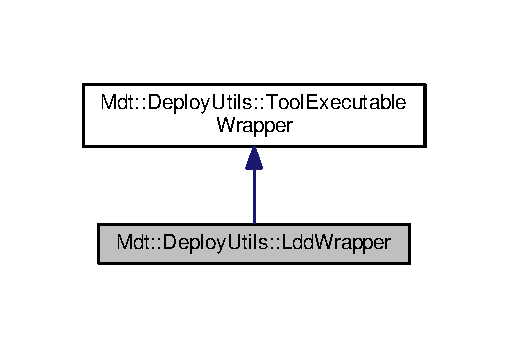
\includegraphics[width=244pt]{class_mdt_1_1_deploy_utils_1_1_ldd_wrapper__inherit__graph}
\end{center}
\end{figure}


Collaboration diagram for Mdt\+:\+:Deploy\+Utils\+:\+:Ldd\+Wrapper\+:\nopagebreak
\begin{figure}[H]
\begin{center}
\leavevmode
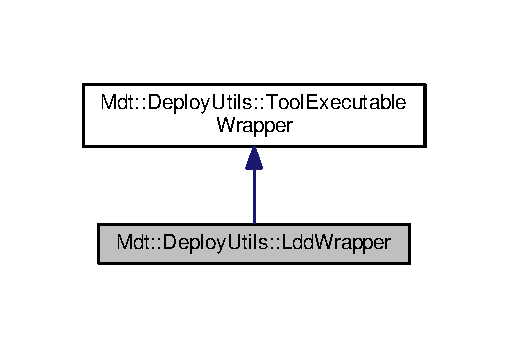
\includegraphics[width=244pt]{class_mdt_1_1_deploy_utils_1_1_ldd_wrapper__coll__graph}
\end{center}
\end{figure}
\subsection*{Public Member Functions}
\begin{DoxyCompactItemize}
\item 
\hyperlink{class_mdt_1_1_deploy_utils_1_1_ldd_wrapper_af06a59c19dd4cff1cd7265d884496ef5}{Ldd\+Wrapper} (Q\+Object $\ast$parent=nullptr)\hypertarget{class_mdt_1_1_deploy_utils_1_1_ldd_wrapper_af06a59c19dd4cff1cd7265d884496ef5}{}\label{class_mdt_1_1_deploy_utils_1_1_ldd_wrapper_af06a59c19dd4cff1cd7265d884496ef5}

\begin{DoxyCompactList}\small\item\em Constructor. \end{DoxyCompactList}\item 
bool \hyperlink{class_mdt_1_1_deploy_utils_1_1_ldd_wrapper_a156c129e6c120c46139cacde66788d92}{exec\+Find\+Dependencies} (const Q\+String \&binary\+File\+Path)
\begin{DoxyCompactList}\small\item\em Execute the command to find dependencies. \end{DoxyCompactList}\end{DoxyCompactItemize}
\subsection*{Additional Inherited Members}


\subsection{Detailed Description}
Wrapps a ldd executable. 

Definition at line 31 of file Ldd\+Wrapper.\+h.



\subsection{Member Function Documentation}
\index{Mdt\+::\+Deploy\+Utils\+::\+Ldd\+Wrapper@{Mdt\+::\+Deploy\+Utils\+::\+Ldd\+Wrapper}!exec\+Find\+Dependencies@{exec\+Find\+Dependencies}}
\index{exec\+Find\+Dependencies@{exec\+Find\+Dependencies}!Mdt\+::\+Deploy\+Utils\+::\+Ldd\+Wrapper@{Mdt\+::\+Deploy\+Utils\+::\+Ldd\+Wrapper}}
\subsubsection[{\texorpdfstring{exec\+Find\+Dependencies(const Q\+String \&binary\+File\+Path)}{execFindDependencies(const QString &binaryFilePath)}}]{\setlength{\rightskip}{0pt plus 5cm}bool Mdt\+::\+Deploy\+Utils\+::\+Ldd\+Wrapper\+::exec\+Find\+Dependencies (
\begin{DoxyParamCaption}
\item[{const Q\+String \&}]{binary\+File\+Path}
\end{DoxyParamCaption}
)}\hypertarget{class_mdt_1_1_deploy_utils_1_1_ldd_wrapper_a156c129e6c120c46139cacde66788d92}{}\label{class_mdt_1_1_deploy_utils_1_1_ldd_wrapper_a156c129e6c120c46139cacde66788d92}


Execute the command to find dependencies. 


\begin{DoxyParams}{Parameters}
{\em binary\+File\+Path} & Path to a executable or a library \\
\hline
\end{DoxyParams}


Definition at line 32 of file Ldd\+Wrapper.\+cpp.



The documentation for this class was generated from the following files\+:\begin{DoxyCompactItemize}
\item 
libs/\+Deploy\+Utils\+\_\+\+Core/src/\+Mdt/\+Deploy\+Utils/Ldd\+Wrapper.\+h\item 
libs/\+Deploy\+Utils\+\_\+\+Core/src/\+Mdt/\+Deploy\+Utils/Ldd\+Wrapper.\+cpp\end{DoxyCompactItemize}

\hypertarget{class_mdt_1_1_numeric_1_1_length}{}\section{Mdt\+:\+:Numeric\+:\+:Length Class Reference}
\label{class_mdt_1_1_numeric_1_1_length}\index{Mdt\+::\+Numeric\+::\+Length@{Mdt\+::\+Numeric\+::\+Length}}


Value type that represents a length.  




{\ttfamily \#include $<$Length.\+h$>$}



Inheritance diagram for Mdt\+:\+:Numeric\+:\+:Length\+:\nopagebreak
\begin{figure}[H]
\begin{center}
\leavevmode
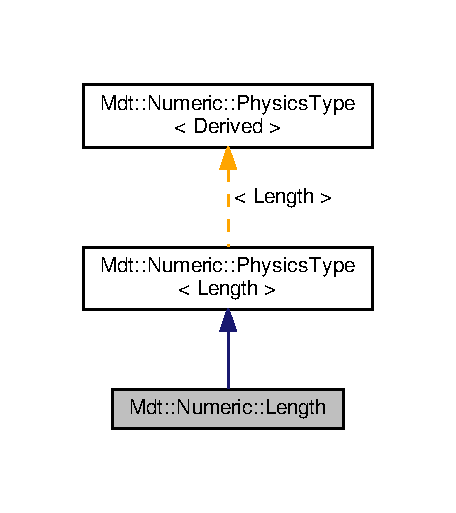
\includegraphics[width=219pt]{class_mdt_1_1_numeric_1_1_length__inherit__graph}
\end{center}
\end{figure}


Collaboration diagram for Mdt\+:\+:Numeric\+:\+:Length\+:\nopagebreak
\begin{figure}[H]
\begin{center}
\leavevmode
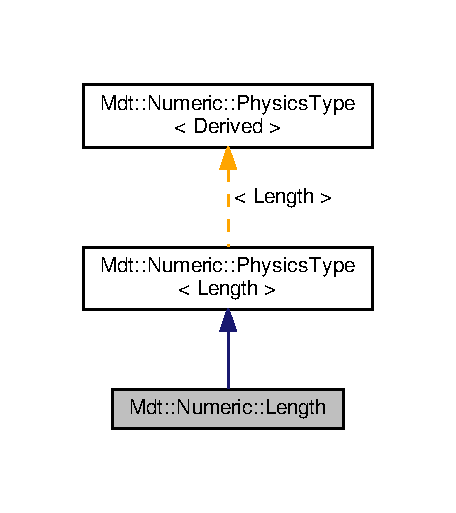
\includegraphics[width=219pt]{class_mdt_1_1_numeric_1_1_length__coll__graph}
\end{center}
\end{figure}
\subsection*{Public Member Functions}
\begin{DoxyCompactItemize}
\item 
constexpr \hyperlink{class_mdt_1_1_numeric_1_1_length_a7ad7b263b98b280ba6d383edc260d2a5}{Length} () noexcept
\begin{DoxyCompactList}\small\item\em Construct a null length. \end{DoxyCompactList}\item 
constexpr \hyperlink{class_mdt_1_1_numeric_1_1_length_a7d7b7aa5f63272a62870dbe782af0adb}{Length} (\hyperlink{class_mdt_1_1_numeric_1_1_double}{Double} l) noexcept
\begin{DoxyCompactList}\small\item\em Construct a length. \end{DoxyCompactList}\item 
constexpr \hyperlink{class_mdt_1_1_numeric_1_1_length_abc975577596b9b57d134ef814ff6a0e4}{Length} (double l) noexcept
\begin{DoxyCompactList}\small\item\em Construct a length. \end{DoxyCompactList}\end{DoxyCompactItemize}
\subsection*{Static Public Member Functions}
\begin{DoxyCompactItemize}
\item 
static \hyperlink{class_mdt_1_1_numeric_1_1_length}{Length} \hyperlink{class_mdt_1_1_numeric_1_1_length_ad4e60674e598aa2dcaec5080b0657e24}{from\+Q\+Variant} (const Q\+Variant \&l)
\begin{DoxyCompactList}\small\item\em Get length from a Q\+Variant. \end{DoxyCompactList}\end{DoxyCompactItemize}


\subsection{Detailed Description}
Value type that represents a length. 

Definition at line 31 of file Length.\+h.



\subsection{Constructor \& Destructor Documentation}
\index{Mdt\+::\+Numeric\+::\+Length@{Mdt\+::\+Numeric\+::\+Length}!Length@{Length}}
\index{Length@{Length}!Mdt\+::\+Numeric\+::\+Length@{Mdt\+::\+Numeric\+::\+Length}}
\subsubsection[{\texorpdfstring{Length() noexcept}{Length() noexcept}}]{\setlength{\rightskip}{0pt plus 5cm}constexpr Mdt\+::\+Numeric\+::\+Length\+::\+Length (
\begin{DoxyParamCaption}
{}
\end{DoxyParamCaption}
)\hspace{0.3cm}{\ttfamily [inline]}, {\ttfamily [noexcept]}}\hypertarget{class_mdt_1_1_numeric_1_1_length_a7ad7b263b98b280ba6d383edc260d2a5}{}\label{class_mdt_1_1_numeric_1_1_length_a7ad7b263b98b280ba6d383edc260d2a5}


Construct a null length. 



Definition at line 37 of file Length.\+h.

\index{Mdt\+::\+Numeric\+::\+Length@{Mdt\+::\+Numeric\+::\+Length}!Length@{Length}}
\index{Length@{Length}!Mdt\+::\+Numeric\+::\+Length@{Mdt\+::\+Numeric\+::\+Length}}
\subsubsection[{\texorpdfstring{Length(\+Double l) noexcept}{Length(Double l) noexcept}}]{\setlength{\rightskip}{0pt plus 5cm}constexpr Mdt\+::\+Numeric\+::\+Length\+::\+Length (
\begin{DoxyParamCaption}
\item[{{\bf Double}}]{l}
\end{DoxyParamCaption}
)\hspace{0.3cm}{\ttfamily [inline]}, {\ttfamily [explicit]}, {\ttfamily [noexcept]}}\hypertarget{class_mdt_1_1_numeric_1_1_length_a7d7b7aa5f63272a62870dbe782af0adb}{}\label{class_mdt_1_1_numeric_1_1_length_a7d7b7aa5f63272a62870dbe782af0adb}


Construct a length. 



Definition at line 42 of file Length.\+h.

\index{Mdt\+::\+Numeric\+::\+Length@{Mdt\+::\+Numeric\+::\+Length}!Length@{Length}}
\index{Length@{Length}!Mdt\+::\+Numeric\+::\+Length@{Mdt\+::\+Numeric\+::\+Length}}
\subsubsection[{\texorpdfstring{Length(double l) noexcept}{Length(double l) noexcept}}]{\setlength{\rightskip}{0pt plus 5cm}constexpr Mdt\+::\+Numeric\+::\+Length\+::\+Length (
\begin{DoxyParamCaption}
\item[{double}]{l}
\end{DoxyParamCaption}
)\hspace{0.3cm}{\ttfamily [inline]}, {\ttfamily [explicit]}, {\ttfamily [noexcept]}}\hypertarget{class_mdt_1_1_numeric_1_1_length_abc975577596b9b57d134ef814ff6a0e4}{}\label{class_mdt_1_1_numeric_1_1_length_abc975577596b9b57d134ef814ff6a0e4}


Construct a length. 



Definition at line 47 of file Length.\+h.



\subsection{Member Function Documentation}
\index{Mdt\+::\+Numeric\+::\+Length@{Mdt\+::\+Numeric\+::\+Length}!from\+Q\+Variant@{from\+Q\+Variant}}
\index{from\+Q\+Variant@{from\+Q\+Variant}!Mdt\+::\+Numeric\+::\+Length@{Mdt\+::\+Numeric\+::\+Length}}
\subsubsection[{\texorpdfstring{from\+Q\+Variant(const Q\+Variant \&l)}{fromQVariant(const QVariant &l)}}]{\setlength{\rightskip}{0pt plus 5cm}static {\bf Length} Mdt\+::\+Numeric\+::\+Length\+::from\+Q\+Variant (
\begin{DoxyParamCaption}
\item[{const Q\+Variant \&}]{l}
\end{DoxyParamCaption}
)\hspace{0.3cm}{\ttfamily [inline]}, {\ttfamily [static]}}\hypertarget{class_mdt_1_1_numeric_1_1_length_ad4e60674e598aa2dcaec5080b0657e24}{}\label{class_mdt_1_1_numeric_1_1_length_ad4e60674e598aa2dcaec5080b0657e24}


Get length from a Q\+Variant. 

If l is null, a null length is returned

\begin{DoxyPrecond}{Precondition}
If l has a value (is not null), it must be convertible to double 
\end{DoxyPrecond}


Definition at line 56 of file Length.\+h.



The documentation for this class was generated from the following file\+:\begin{DoxyCompactItemize}
\item 
libs/\+Numeric/src/\+Mdt/\+Numeric/Length.\+h\end{DoxyCompactItemize}

\hypertarget{class_mdt_1_1_deploy_utils_1_1_library}{}\section{Mdt\+:\+:Deploy\+Utils\+:\+:Library Class Reference}
\label{class_mdt_1_1_deploy_utils_1_1_library}\index{Mdt\+::\+Deploy\+Utils\+::\+Library@{Mdt\+::\+Deploy\+Utils\+::\+Library}}


Provides some helper methods for libraries.  




{\ttfamily \#include $<$Library.\+h$>$}



Inheritance diagram for Mdt\+:\+:Deploy\+Utils\+:\+:Library\+:
\nopagebreak
\begin{figure}[H]
\begin{center}
\leavevmode
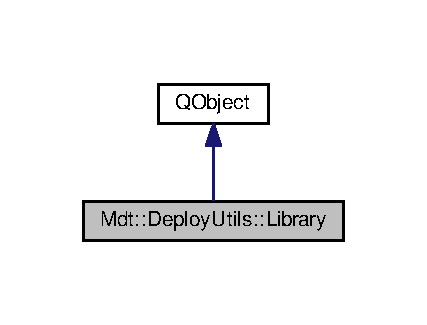
\includegraphics[width=205pt]{class_mdt_1_1_deploy_utils_1_1_library__inherit__graph}
\end{center}
\end{figure}


Collaboration diagram for Mdt\+:\+:Deploy\+Utils\+:\+:Library\+:
\nopagebreak
\begin{figure}[H]
\begin{center}
\leavevmode
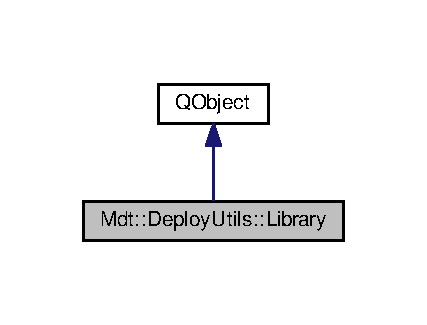
\includegraphics[width=205pt]{class_mdt_1_1_deploy_utils_1_1_library__coll__graph}
\end{center}
\end{figure}
\subsection*{Public Types}
\begin{DoxyCompactItemize}
\item 
enum \hyperlink{class_mdt_1_1_deploy_utils_1_1_library_ab9f58dba8290dd1882a21d73cc7c10d0}{Search\+In\+System\+Paths} \{ \hyperlink{class_mdt_1_1_deploy_utils_1_1_library_ab9f58dba8290dd1882a21d73cc7c10d0adabc8cd036aa884536c359cc3a2783ca}{Include\+System\+Paths}, 
\hyperlink{class_mdt_1_1_deploy_utils_1_1_library_ab9f58dba8290dd1882a21d73cc7c10d0ad00095fee49be0d8f0e8c7467dc8ebec}{Exclude\+System\+Paths}
 \}\begin{DoxyCompactList}\small\item\em Tell if search must include system paths or not. \end{DoxyCompactList}
\end{DoxyCompactItemize}
\subsection*{Public Member Functions}
\begin{DoxyCompactItemize}
\item 
\hyperlink{class_mdt_1_1_deploy_utils_1_1_library_ae3d859ad862e026b00d12e50702ae4df}{Library} (\hyperlink{class_q_object}{Q\+Object} $\ast$parent=nullptr)
\begin{DoxyCompactList}\small\item\em Constructor. \end{DoxyCompactList}\item 
{\bfseries Library} (const \hyperlink{class_mdt_1_1_deploy_utils_1_1_library}{Library} \&)=delete\hypertarget{class_mdt_1_1_deploy_utils_1_1_library_a8c0856517a687937d59df6d0776a6cc8}{}\label{class_mdt_1_1_deploy_utils_1_1_library_a8c0856517a687937d59df6d0776a6cc8}

\item 
\hyperlink{class_mdt_1_1_deploy_utils_1_1_library}{Library} \& {\bfseries operator=} (const \hyperlink{class_mdt_1_1_deploy_utils_1_1_library}{Library} \&)=delete\hypertarget{class_mdt_1_1_deploy_utils_1_1_library_aa024a19c0cd43f2523ece558093a7dbb}{}\label{class_mdt_1_1_deploy_utils_1_1_library_aa024a19c0cd43f2523ece558093a7dbb}

\item 
{\bfseries Library} (\hyperlink{class_mdt_1_1_deploy_utils_1_1_library}{Library} \&\&)=delete\hypertarget{class_mdt_1_1_deploy_utils_1_1_library_ab3ef2a8f7f154733f5a79191ceaaa185}{}\label{class_mdt_1_1_deploy_utils_1_1_library_ab3ef2a8f7f154733f5a79191ceaaa185}

\item 
\hyperlink{class_mdt_1_1_deploy_utils_1_1_library}{Library} \& {\bfseries operator=} (\hyperlink{class_mdt_1_1_deploy_utils_1_1_library}{Library} \&\&)=delete\hypertarget{class_mdt_1_1_deploy_utils_1_1_library_afbe16dc9aeff2acc7964db4b447117d9}{}\label{class_mdt_1_1_deploy_utils_1_1_library_afbe16dc9aeff2acc7964db4b447117d9}

\item 
bool \hyperlink{class_mdt_1_1_deploy_utils_1_1_library_afeac04ff3404387fc542347849bffeb4}{find\+Library} (const Q\+String \&name, const \hyperlink{class_mdt_1_1_deploy_utils_1_1_path_list}{Path\+List} path\+List=\hyperlink{class_mdt_1_1_deploy_utils_1_1_path_list}{Path\+List}(), \hyperlink{class_mdt_1_1_deploy_utils_1_1_library_ab9f58dba8290dd1882a21d73cc7c10d0}{Search\+In\+System\+Paths} search\+In\+System\+Paths=\hyperlink{class_mdt_1_1_deploy_utils_1_1_library_ab9f58dba8290dd1882a21d73cc7c10d0adabc8cd036aa884536c359cc3a2783ca}{Include\+System\+Paths})
\begin{DoxyCompactList}\small\item\em Find a library. \end{DoxyCompactList}\item 
\hyperlink{class_mdt_1_1_deploy_utils_1_1_library_info}{Library\+Info} \hyperlink{class_mdt_1_1_deploy_utils_1_1_library_a8b272e0c638aa2949b5f19b3c75ed9ae}{library\+Info} () const 
\begin{DoxyCompactList}\small\item\em Get library info. \end{DoxyCompactList}\item 
\hyperlink{class_mdt_1_1_error}{Mdt\+::\+Error} \hyperlink{class_mdt_1_1_deploy_utils_1_1_library_adb9bf35bba0d23731ac97d40fc5fe91d}{last\+Error} () const 
\begin{DoxyCompactList}\small\item\em Get last error. \end{DoxyCompactList}\end{DoxyCompactItemize}


\subsection{Detailed Description}
Provides some helper methods for libraries. 

Definition at line 34 of file Library.\+h.



\subsection{Member Enumeration Documentation}
\index{Mdt\+::\+Deploy\+Utils\+::\+Library@{Mdt\+::\+Deploy\+Utils\+::\+Library}!Search\+In\+System\+Paths@{Search\+In\+System\+Paths}}
\index{Search\+In\+System\+Paths@{Search\+In\+System\+Paths}!Mdt\+::\+Deploy\+Utils\+::\+Library@{Mdt\+::\+Deploy\+Utils\+::\+Library}}
\subsubsection[{\texorpdfstring{Search\+In\+System\+Paths}{SearchInSystemPaths}}]{\setlength{\rightskip}{0pt plus 5cm}enum {\bf Mdt\+::\+Deploy\+Utils\+::\+Library\+::\+Search\+In\+System\+Paths}}\hypertarget{class_mdt_1_1_deploy_utils_1_1_library_ab9f58dba8290dd1882a21d73cc7c10d0}{}\label{class_mdt_1_1_deploy_utils_1_1_library_ab9f58dba8290dd1882a21d73cc7c10d0}


Tell if search must include system paths or not. 

\begin{Desc}
\item[Enumerator]\par
\begin{description}
\index{Include\+System\+Paths@{Include\+System\+Paths}!Mdt\+::\+Deploy\+Utils\+::\+Library@{Mdt\+::\+Deploy\+Utils\+::\+Library}}\index{Mdt\+::\+Deploy\+Utils\+::\+Library@{Mdt\+::\+Deploy\+Utils\+::\+Library}!Include\+System\+Paths@{Include\+System\+Paths}}\item[{\em 
Include\+System\+Paths\hypertarget{class_mdt_1_1_deploy_utils_1_1_library_ab9f58dba8290dd1882a21d73cc7c10d0adabc8cd036aa884536c359cc3a2783ca}{}\label{class_mdt_1_1_deploy_utils_1_1_library_ab9f58dba8290dd1882a21d73cc7c10d0adabc8cd036aa884536c359cc3a2783ca}
}]Also search in system path \index{Exclude\+System\+Paths@{Exclude\+System\+Paths}!Mdt\+::\+Deploy\+Utils\+::\+Library@{Mdt\+::\+Deploy\+Utils\+::\+Library}}\index{Mdt\+::\+Deploy\+Utils\+::\+Library@{Mdt\+::\+Deploy\+Utils\+::\+Library}!Exclude\+System\+Paths@{Exclude\+System\+Paths}}\item[{\em 
Exclude\+System\+Paths\hypertarget{class_mdt_1_1_deploy_utils_1_1_library_ab9f58dba8290dd1882a21d73cc7c10d0ad00095fee49be0d8f0e8c7467dc8ebec}{}\label{class_mdt_1_1_deploy_utils_1_1_library_ab9f58dba8290dd1882a21d73cc7c10d0ad00095fee49be0d8f0e8c7467dc8ebec}
}]Do not search in system path \end{description}
\end{Desc}


Definition at line 42 of file Library.\+h.



\subsection{Constructor \& Destructor Documentation}
\index{Mdt\+::\+Deploy\+Utils\+::\+Library@{Mdt\+::\+Deploy\+Utils\+::\+Library}!Library@{Library}}
\index{Library@{Library}!Mdt\+::\+Deploy\+Utils\+::\+Library@{Mdt\+::\+Deploy\+Utils\+::\+Library}}
\subsubsection[{\texorpdfstring{Library(\+Q\+Object $\ast$parent=nullptr)}{Library(QObject *parent=nullptr)}}]{\setlength{\rightskip}{0pt plus 5cm}Mdt\+::\+Deploy\+Utils\+::\+Library\+::\+Library (
\begin{DoxyParamCaption}
\item[{{\bf Q\+Object} $\ast$}]{parent = {\ttfamily nullptr}}
\end{DoxyParamCaption}
)\hspace{0.3cm}{\ttfamily [explicit]}}\hypertarget{class_mdt_1_1_deploy_utils_1_1_library_ae3d859ad862e026b00d12e50702ae4df}{}\label{class_mdt_1_1_deploy_utils_1_1_library_ae3d859ad862e026b00d12e50702ae4df}


Constructor. 



Definition at line 32 of file Library.\+cpp.



\subsection{Member Function Documentation}
\index{Mdt\+::\+Deploy\+Utils\+::\+Library@{Mdt\+::\+Deploy\+Utils\+::\+Library}!find\+Library@{find\+Library}}
\index{find\+Library@{find\+Library}!Mdt\+::\+Deploy\+Utils\+::\+Library@{Mdt\+::\+Deploy\+Utils\+::\+Library}}
\subsubsection[{\texorpdfstring{find\+Library(const Q\+String \&name, const Path\+List path\+List=\+Path\+List(), Search\+In\+System\+Paths search\+In\+System\+Paths=\+Include\+System\+Paths)}{findLibrary(const QString &name, const PathList pathList=PathList(), SearchInSystemPaths searchInSystemPaths=IncludeSystemPaths)}}]{\setlength{\rightskip}{0pt plus 5cm}bool Mdt\+::\+Deploy\+Utils\+::\+Library\+::find\+Library (
\begin{DoxyParamCaption}
\item[{const Q\+String \&}]{name, }
\item[{const {\bf Path\+List}}]{path\+List = {\ttfamily {\bf Path\+List}()}, }
\item[{{\bf Library\+::\+Search\+In\+System\+Paths}}]{search\+In\+System\+Paths = {\ttfamily {\bf Include\+System\+Paths}}}
\end{DoxyParamCaption}
)}\hypertarget{class_mdt_1_1_deploy_utils_1_1_library_afeac04ff3404387fc542347849bffeb4}{}\label{class_mdt_1_1_deploy_utils_1_1_library_afeac04ff3404387fc542347849bffeb4}


Find a library. 


\begin{DoxyParams}{Parameters}
{\em name} & Name of the library. Can be a name without any prefix or suffix (ex\+: Qt5\+Core), or a more platform specific name (ex\+: lib\+Qt5\+Core.\+so). For platform that supports versions in the library file name, a versionned name can be done (ex\+: lib\+Qt5\+Core.\+so.\+5 , lib\+Qt5\+Core.\+so.\+5.\+6.\+2) \\
\hline
{\em path\+List} & List of paths where to search the library \\
\hline
{\em search\+In\+System\+Paths} & Tell if the search must include system paths \\
\hline
\end{DoxyParams}
\begin{DoxyReturn}{Returns}
True if the library was found, false if it was not found, or a error occured. 
\end{DoxyReturn}
\begin{DoxyPrecond}{Precondition}
name must be a non empty string. 

If {\itshape search\+In\+System\+Paths} is Exclude\+System\+Paths, path\+List must contain at least 1 path 
\end{DoxyPrecond}


Definition at line 37 of file Library.\+cpp.

\index{Mdt\+::\+Deploy\+Utils\+::\+Library@{Mdt\+::\+Deploy\+Utils\+::\+Library}!last\+Error@{last\+Error}}
\index{last\+Error@{last\+Error}!Mdt\+::\+Deploy\+Utils\+::\+Library@{Mdt\+::\+Deploy\+Utils\+::\+Library}}
\subsubsection[{\texorpdfstring{last\+Error() const }{lastError() const }}]{\setlength{\rightskip}{0pt plus 5cm}{\bf Mdt\+::\+Error} Mdt\+::\+Deploy\+Utils\+::\+Library\+::last\+Error (
\begin{DoxyParamCaption}
{}
\end{DoxyParamCaption}
) const\hspace{0.3cm}{\ttfamily [inline]}}\hypertarget{class_mdt_1_1_deploy_utils_1_1_library_adb9bf35bba0d23731ac97d40fc5fe91d}{}\label{class_mdt_1_1_deploy_utils_1_1_library_adb9bf35bba0d23731ac97d40fc5fe91d}


Get last error. 



Definition at line 86 of file Library.\+h.

\index{Mdt\+::\+Deploy\+Utils\+::\+Library@{Mdt\+::\+Deploy\+Utils\+::\+Library}!library\+Info@{library\+Info}}
\index{library\+Info@{library\+Info}!Mdt\+::\+Deploy\+Utils\+::\+Library@{Mdt\+::\+Deploy\+Utils\+::\+Library}}
\subsubsection[{\texorpdfstring{library\+Info() const }{libraryInfo() const }}]{\setlength{\rightskip}{0pt plus 5cm}{\bf Library\+Info} Mdt\+::\+Deploy\+Utils\+::\+Library\+::library\+Info (
\begin{DoxyParamCaption}
{}
\end{DoxyParamCaption}
) const\hspace{0.3cm}{\ttfamily [inline]}}\hypertarget{class_mdt_1_1_deploy_utils_1_1_library_a8b272e0c638aa2949b5f19b3c75ed9ae}{}\label{class_mdt_1_1_deploy_utils_1_1_library_a8b272e0c638aa2949b5f19b3c75ed9ae}


Get library info. 

Returns the information of the library after a success call of \hyperlink{class_mdt_1_1_deploy_utils_1_1_library_afeac04ff3404387fc542347849bffeb4}{find\+Library()} 

Definition at line 79 of file Library.\+h.



The documentation for this class was generated from the following files\+:\begin{DoxyCompactItemize}
\item 
libs/\+Deploy\+Utils\+\_\+\+Core/src/\+Mdt/\+Deploy\+Utils/Library.\+h\item 
libs/\+Deploy\+Utils\+\_\+\+Core/src/\+Mdt/\+Deploy\+Utils/Library.\+cpp\end{DoxyCompactItemize}

\hypertarget{class_mdt_1_1_deploy_utils_1_1_library_info}{}\section{Mdt\+:\+:Deploy\+Utils\+:\+:Library\+Info Class Reference}
\label{class_mdt_1_1_deploy_utils_1_1_library_info}\index{Mdt\+::\+Deploy\+Utils\+::\+Library\+Info@{Mdt\+::\+Deploy\+Utils\+::\+Library\+Info}}


Data value class that stores informations about a library.  




{\ttfamily \#include $<$Library\+Info.\+h$>$}

\subsection*{Public Member Functions}
\begin{DoxyCompactItemize}
\item 
void \hyperlink{class_mdt_1_1_deploy_utils_1_1_library_info_a0b7af709bcbd3c3b7f22e954d11ff812}{set\+Absolute\+File\+Path} (const Q\+String \&path)\hypertarget{class_mdt_1_1_deploy_utils_1_1_library_info_a0b7af709bcbd3c3b7f22e954d11ff812}{}\label{class_mdt_1_1_deploy_utils_1_1_library_info_a0b7af709bcbd3c3b7f22e954d11ff812}

\begin{DoxyCompactList}\small\item\em Set absolute file path. \end{DoxyCompactList}\item 
Q\+String \hyperlink{class_mdt_1_1_deploy_utils_1_1_library_info_a698bb904c4bbb50034b0a47f68c1c89a}{absolute\+File\+Path} () const \hypertarget{class_mdt_1_1_deploy_utils_1_1_library_info_a698bb904c4bbb50034b0a47f68c1c89a}{}\label{class_mdt_1_1_deploy_utils_1_1_library_info_a698bb904c4bbb50034b0a47f68c1c89a}

\begin{DoxyCompactList}\small\item\em Get absolute file path. \end{DoxyCompactList}\item 
void \hyperlink{class_mdt_1_1_deploy_utils_1_1_library_info_aaa4bbfc9f8640f3d152e59c4e7763cf2}{set\+Library\+Platform\+Name} (const Q\+String \&name)
\begin{DoxyCompactList}\small\item\em Set library name. \end{DoxyCompactList}\item 
void \hyperlink{class_mdt_1_1_deploy_utils_1_1_library_info_acd5102f7ca77e51efde466342b27f0ce}{set\+Library\+Name} (const \hyperlink{class_mdt_1_1_deploy_utils_1_1_library_name}{Library\+Name} \&\hyperlink{class_mdt_1_1_deploy_utils_1_1_library_info_a6d3a8bd86079dfe21b3e1fcde3d6e068}{library\+Name})
\begin{DoxyCompactList}\small\item\em Set library name. \end{DoxyCompactList}\item 
\hyperlink{class_mdt_1_1_deploy_utils_1_1_library_name}{Library\+Name} \hyperlink{class_mdt_1_1_deploy_utils_1_1_library_info_a6d3a8bd86079dfe21b3e1fcde3d6e068}{library\+Name} () const \hypertarget{class_mdt_1_1_deploy_utils_1_1_library_info_a6d3a8bd86079dfe21b3e1fcde3d6e068}{}\label{class_mdt_1_1_deploy_utils_1_1_library_info_a6d3a8bd86079dfe21b3e1fcde3d6e068}

\begin{DoxyCompactList}\small\item\em Get library name. \end{DoxyCompactList}\item 
bool \hyperlink{class_mdt_1_1_deploy_utils_1_1_library_info_a4a48fdaaeb10412441f4e1edddfd1026}{is\+Null} () const \hypertarget{class_mdt_1_1_deploy_utils_1_1_library_info_a4a48fdaaeb10412441f4e1edddfd1026}{}\label{class_mdt_1_1_deploy_utils_1_1_library_info_a4a48fdaaeb10412441f4e1edddfd1026}

\begin{DoxyCompactList}\small\item\em Check if this library info is null. \end{DoxyCompactList}\end{DoxyCompactItemize}
\subsection*{Friends}
\begin{DoxyCompactItemize}
\item 
bool \hyperlink{class_mdt_1_1_deploy_utils_1_1_library_info_ac6f255170448e5789db860534a4eddbe}{operator==} (const \hyperlink{class_mdt_1_1_deploy_utils_1_1_library_info}{Library\+Info} \&a, const \hyperlink{class_mdt_1_1_deploy_utils_1_1_library_info}{Library\+Info} \&b)\hypertarget{class_mdt_1_1_deploy_utils_1_1_library_info_ac6f255170448e5789db860534a4eddbe}{}\label{class_mdt_1_1_deploy_utils_1_1_library_info_ac6f255170448e5789db860534a4eddbe}

\begin{DoxyCompactList}\small\item\em Check if library info a and b are equal. \end{DoxyCompactList}\item 
bool \hyperlink{class_mdt_1_1_deploy_utils_1_1_library_info_a4888aa068e25a386597525dabcbdbb97}{operator!=} (const \hyperlink{class_mdt_1_1_deploy_utils_1_1_library_info}{Library\+Info} \&a, const \hyperlink{class_mdt_1_1_deploy_utils_1_1_library_info}{Library\+Info} \&b)\hypertarget{class_mdt_1_1_deploy_utils_1_1_library_info_a4888aa068e25a386597525dabcbdbb97}{}\label{class_mdt_1_1_deploy_utils_1_1_library_info_a4888aa068e25a386597525dabcbdbb97}

\begin{DoxyCompactList}\small\item\em Check if library info a and b are different. \end{DoxyCompactList}\end{DoxyCompactItemize}


\subsection{Detailed Description}
Data value class that stores informations about a library. 

Definition at line 34 of file Library\+Info.\+h.



\subsection{Member Function Documentation}
\index{Mdt\+::\+Deploy\+Utils\+::\+Library\+Info@{Mdt\+::\+Deploy\+Utils\+::\+Library\+Info}!set\+Library\+Name@{set\+Library\+Name}}
\index{set\+Library\+Name@{set\+Library\+Name}!Mdt\+::\+Deploy\+Utils\+::\+Library\+Info@{Mdt\+::\+Deploy\+Utils\+::\+Library\+Info}}
\subsubsection[{\texorpdfstring{set\+Library\+Name(const Library\+Name \&library\+Name)}{setLibraryName(const LibraryName &libraryName)}}]{\setlength{\rightskip}{0pt plus 5cm}void Mdt\+::\+Deploy\+Utils\+::\+Library\+Info\+::set\+Library\+Name (
\begin{DoxyParamCaption}
\item[{const {\bf Library\+Name} \&}]{library\+Name}
\end{DoxyParamCaption}
)}\hypertarget{class_mdt_1_1_deploy_utils_1_1_library_info_acd5102f7ca77e51efde466342b27f0ce}{}\label{class_mdt_1_1_deploy_utils_1_1_library_info_acd5102f7ca77e51efde466342b27f0ce}


Set library name. 

\begin{DoxySeeAlso}{See also}
\hyperlink{class_mdt_1_1_deploy_utils_1_1_library_name}{Library\+Name} 
\end{DoxySeeAlso}


Definition at line 38 of file Library\+Info.\+cpp.

\index{Mdt\+::\+Deploy\+Utils\+::\+Library\+Info@{Mdt\+::\+Deploy\+Utils\+::\+Library\+Info}!set\+Library\+Platform\+Name@{set\+Library\+Platform\+Name}}
\index{set\+Library\+Platform\+Name@{set\+Library\+Platform\+Name}!Mdt\+::\+Deploy\+Utils\+::\+Library\+Info@{Mdt\+::\+Deploy\+Utils\+::\+Library\+Info}}
\subsubsection[{\texorpdfstring{set\+Library\+Platform\+Name(const Q\+String \&name)}{setLibraryPlatformName(const QString &name)}}]{\setlength{\rightskip}{0pt plus 5cm}void Mdt\+::\+Deploy\+Utils\+::\+Library\+Info\+::set\+Library\+Platform\+Name (
\begin{DoxyParamCaption}
\item[{const Q\+String \&}]{name}
\end{DoxyParamCaption}
)}\hypertarget{class_mdt_1_1_deploy_utils_1_1_library_info_aaa4bbfc9f8640f3d152e59c4e7763cf2}{}\label{class_mdt_1_1_deploy_utils_1_1_library_info_aaa4bbfc9f8640f3d152e59c4e7763cf2}


Set library name. 

{\itshape name} should be the full library file name (f.\+ex. lib\+Qt5\+Core.\+so, or Qt5\+Core.\+dll). To specify only the library name (like Qt5\+Core), use \hyperlink{class_mdt_1_1_deploy_utils_1_1_library_info_acd5102f7ca77e51efde466342b27f0ce}{set\+Library\+Name()}.

\begin{DoxyPrecond}{Precondition}
{\itshape name} must at least have a library name and a extension. 
\end{DoxyPrecond}


Definition at line 30 of file Library\+Info.\+cpp.



The documentation for this class was generated from the following files\+:\begin{DoxyCompactItemize}
\item 
libs/\+Deploy\+Utils\+\_\+\+Core/src/\+Mdt/\+Deploy\+Utils/Library\+Info.\+h\item 
libs/\+Deploy\+Utils\+\_\+\+Core/src/\+Mdt/\+Deploy\+Utils/Library\+Info.\+cpp\end{DoxyCompactItemize}

\hypertarget{class_mdt_1_1_deploy_utils_1_1_library_info_list}{}\section{Mdt\+:\+:Deploy\+Utils\+:\+:Library\+Info\+List Class Reference}
\label{class_mdt_1_1_deploy_utils_1_1_library_info_list}\index{Mdt\+::\+Deploy\+Utils\+::\+Library\+Info\+List@{Mdt\+::\+Deploy\+Utils\+::\+Library\+Info\+List}}


Container that holds a list of \hyperlink{class_mdt_1_1_deploy_utils_1_1_library_info}{Library\+Info}.  




{\ttfamily \#include $<$Library\+Info\+List.\+h$>$}

\subsection*{Public Types}
\begin{DoxyCompactItemize}
\item 
using \hyperlink{class_mdt_1_1_deploy_utils_1_1_library_info_list_a07338b20f243a1c7fcb3f696a35ddd44}{const\+\_\+iterator} = Q\+Vector$<$ \hyperlink{class_mdt_1_1_deploy_utils_1_1_library_info}{Library\+Info} $>$\+::\hyperlink{class_mdt_1_1_deploy_utils_1_1_library_info_list_a07338b20f243a1c7fcb3f696a35ddd44}{const\+\_\+iterator}\hypertarget{class_mdt_1_1_deploy_utils_1_1_library_info_list_a07338b20f243a1c7fcb3f696a35ddd44}{}\label{class_mdt_1_1_deploy_utils_1_1_library_info_list_a07338b20f243a1c7fcb3f696a35ddd44}

\begin{DoxyCompactList}\small\item\em S\+T\+L-\/style const iterator. \end{DoxyCompactList}\item 
using \hyperlink{class_mdt_1_1_deploy_utils_1_1_library_info_list_afcdf2c32ca02273dd257814517b691e8}{value\+\_\+type} = Q\+Vector$<$ \hyperlink{class_mdt_1_1_deploy_utils_1_1_library_info}{Library\+Info} $>$\+::\hyperlink{class_mdt_1_1_deploy_utils_1_1_library_info_list_afcdf2c32ca02273dd257814517b691e8}{value\+\_\+type}\hypertarget{class_mdt_1_1_deploy_utils_1_1_library_info_list_afcdf2c32ca02273dd257814517b691e8}{}\label{class_mdt_1_1_deploy_utils_1_1_library_info_list_afcdf2c32ca02273dd257814517b691e8}

\begin{DoxyCompactList}\small\item\em S\+TL value type. \end{DoxyCompactList}\end{DoxyCompactItemize}
\subsection*{Public Member Functions}
\begin{DoxyCompactItemize}
\item 
\hyperlink{class_mdt_1_1_deploy_utils_1_1_library_info_list_a3157bd9fc09a3472c1a0e2e615d619ea}{Library\+Info\+List} ()=default\hypertarget{class_mdt_1_1_deploy_utils_1_1_library_info_list_a3157bd9fc09a3472c1a0e2e615d619ea}{}\label{class_mdt_1_1_deploy_utils_1_1_library_info_list_a3157bd9fc09a3472c1a0e2e615d619ea}

\begin{DoxyCompactList}\small\item\em Construct a empty library info list. \end{DoxyCompactList}\item 
\hyperlink{class_mdt_1_1_deploy_utils_1_1_library_info_list_ad7855d64a98e84a8ae1cf71acf03dbc4}{Library\+Info\+List} (std\+::initializer\+\_\+list$<$ \hyperlink{class_mdt_1_1_deploy_utils_1_1_library_info}{Library\+Info} $>$ list)\hypertarget{class_mdt_1_1_deploy_utils_1_1_library_info_list_ad7855d64a98e84a8ae1cf71acf03dbc4}{}\label{class_mdt_1_1_deploy_utils_1_1_library_info_list_ad7855d64a98e84a8ae1cf71acf03dbc4}

\begin{DoxyCompactList}\small\item\em Construct a library info list from initializer lists. \end{DoxyCompactList}\item 
\hyperlink{class_mdt_1_1_deploy_utils_1_1_library_info_list_ab96b187fdc2f20b37aee8786018a4675}{Library\+Info\+List} (const \hyperlink{class_mdt_1_1_deploy_utils_1_1_library_info_list}{Library\+Info\+List} \&)=default\hypertarget{class_mdt_1_1_deploy_utils_1_1_library_info_list_ab96b187fdc2f20b37aee8786018a4675}{}\label{class_mdt_1_1_deploy_utils_1_1_library_info_list_ab96b187fdc2f20b37aee8786018a4675}

\begin{DoxyCompactList}\small\item\em Copy construct a library info list from a other. \end{DoxyCompactList}\item 
\hyperlink{class_mdt_1_1_deploy_utils_1_1_library_info_list}{Library\+Info\+List} \& \hyperlink{class_mdt_1_1_deploy_utils_1_1_library_info_list_a3f6c7292e77383705324a45b26c2240f}{operator=} (const \hyperlink{class_mdt_1_1_deploy_utils_1_1_library_info_list}{Library\+Info\+List} \&)=default\hypertarget{class_mdt_1_1_deploy_utils_1_1_library_info_list_a3f6c7292e77383705324a45b26c2240f}{}\label{class_mdt_1_1_deploy_utils_1_1_library_info_list_a3f6c7292e77383705324a45b26c2240f}

\begin{DoxyCompactList}\small\item\em Copy assign a library info list this this one. \end{DoxyCompactList}\item 
\hyperlink{class_mdt_1_1_deploy_utils_1_1_library_info_list_a81366014bcc6c3e6577e52bbe42f0893}{Library\+Info\+List} (\hyperlink{class_mdt_1_1_deploy_utils_1_1_library_info_list}{Library\+Info\+List} \&\&)=default\hypertarget{class_mdt_1_1_deploy_utils_1_1_library_info_list_a81366014bcc6c3e6577e52bbe42f0893}{}\label{class_mdt_1_1_deploy_utils_1_1_library_info_list_a81366014bcc6c3e6577e52bbe42f0893}

\begin{DoxyCompactList}\small\item\em Move construct a library info list from a other. \end{DoxyCompactList}\item 
\hyperlink{class_mdt_1_1_deploy_utils_1_1_library_info_list}{Library\+Info\+List} \& \hyperlink{class_mdt_1_1_deploy_utils_1_1_library_info_list_a6c572a7666d521fec0aadc0ac1b6ed92}{operator=} (\hyperlink{class_mdt_1_1_deploy_utils_1_1_library_info_list}{Library\+Info\+List} \&\&)=default\hypertarget{class_mdt_1_1_deploy_utils_1_1_library_info_list_a6c572a7666d521fec0aadc0ac1b6ed92}{}\label{class_mdt_1_1_deploy_utils_1_1_library_info_list_a6c572a7666d521fec0aadc0ac1b6ed92}

\begin{DoxyCompactList}\small\item\em Move assign a library info list this this one. \end{DoxyCompactList}\item 
void \hyperlink{class_mdt_1_1_deploy_utils_1_1_library_info_list_a2fd0bcb2c98ed5a9587e54d6496dac14}{add\+Library} (const \hyperlink{class_mdt_1_1_deploy_utils_1_1_library_info}{Library\+Info} \&library)
\begin{DoxyCompactList}\small\item\em Add a library info to the end of this list. \end{DoxyCompactList}\item 
void \hyperlink{class_mdt_1_1_deploy_utils_1_1_library_info_list_ab2b6f563946dbd690155c7b46e5b94c0}{push\+\_\+back} (const \hyperlink{class_mdt_1_1_deploy_utils_1_1_library_info}{Library\+Info} \&library)
\begin{DoxyCompactList}\small\item\em Add a library info to the end of this list. \end{DoxyCompactList}\item 
void \hyperlink{class_mdt_1_1_deploy_utils_1_1_library_info_list_a08bddbe73a73a1c3b11c1d7633d4ca5c}{add\+Libraries} (const \hyperlink{class_mdt_1_1_deploy_utils_1_1_library_info_list}{Library\+Info\+List} \&libraries)
\begin{DoxyCompactList}\small\item\em Add a list of libraries to this list. \end{DoxyCompactList}\item 
int \hyperlink{class_mdt_1_1_deploy_utils_1_1_library_info_list_a4a43a85999332ac32f738342fc8d832a}{count} () const \hypertarget{class_mdt_1_1_deploy_utils_1_1_library_info_list_a4a43a85999332ac32f738342fc8d832a}{}\label{class_mdt_1_1_deploy_utils_1_1_library_info_list_a4a43a85999332ac32f738342fc8d832a}

\begin{DoxyCompactList}\small\item\em Get count of items in this list. \end{DoxyCompactList}\item 
bool \hyperlink{class_mdt_1_1_deploy_utils_1_1_library_info_list_a3868a02a4c0d4836f9c90fabde0213db}{is\+Empty} () const \hypertarget{class_mdt_1_1_deploy_utils_1_1_library_info_list_a3868a02a4c0d4836f9c90fabde0213db}{}\label{class_mdt_1_1_deploy_utils_1_1_library_info_list_a3868a02a4c0d4836f9c90fabde0213db}

\begin{DoxyCompactList}\small\item\em Check if this list is empty. \end{DoxyCompactList}\item 
bool \hyperlink{class_mdt_1_1_deploy_utils_1_1_library_info_list_a2bdcf5564dd1846be16fc5544120fe03}{contains\+Library\+Absolute\+File\+Path} (const Q\+String \&file\+Path) const \hypertarget{class_mdt_1_1_deploy_utils_1_1_library_info_list_a2bdcf5564dd1846be16fc5544120fe03}{}\label{class_mdt_1_1_deploy_utils_1_1_library_info_list_a2bdcf5564dd1846be16fc5544120fe03}

\begin{DoxyCompactList}\small\item\em Check if this list contains library. \end{DoxyCompactList}\item 
const \hyperlink{class_mdt_1_1_deploy_utils_1_1_library_info}{Library\+Info} \& \hyperlink{class_mdt_1_1_deploy_utils_1_1_library_info_list_a9c8d42963dc6318d45d90f3e63aa5569}{at} (int index) const 
\begin{DoxyCompactList}\small\item\em Get library info list at index. \end{DoxyCompactList}\item 
void \hyperlink{class_mdt_1_1_deploy_utils_1_1_library_info_list_ac6d89745bccdd70bcf08d5bbe6f9a539}{clear} ()\hypertarget{class_mdt_1_1_deploy_utils_1_1_library_info_list_ac6d89745bccdd70bcf08d5bbe6f9a539}{}\label{class_mdt_1_1_deploy_utils_1_1_library_info_list_ac6d89745bccdd70bcf08d5bbe6f9a539}

\begin{DoxyCompactList}\small\item\em Clear this list. \end{DoxyCompactList}\item 
void \hyperlink{class_mdt_1_1_deploy_utils_1_1_library_info_list_ab98b4f9f2c911281467301b4c4a485f2}{reserve} (int size)\hypertarget{class_mdt_1_1_deploy_utils_1_1_library_info_list_ab98b4f9f2c911281467301b4c4a485f2}{}\label{class_mdt_1_1_deploy_utils_1_1_library_info_list_ab98b4f9f2c911281467301b4c4a485f2}

\begin{DoxyCompactList}\small\item\em Attempts to allocate memory for at least size elements. \end{DoxyCompactList}\item 
\hyperlink{class_mdt_1_1_deploy_utils_1_1_library_info_list_a07338b20f243a1c7fcb3f696a35ddd44}{const\+\_\+iterator} \hyperlink{class_mdt_1_1_deploy_utils_1_1_library_info_list_a3e40ff4b11d26a0e2acecc7aaf78248b}{cbegin} () const \hypertarget{class_mdt_1_1_deploy_utils_1_1_library_info_list_a3e40ff4b11d26a0e2acecc7aaf78248b}{}\label{class_mdt_1_1_deploy_utils_1_1_library_info_list_a3e40ff4b11d26a0e2acecc7aaf78248b}

\begin{DoxyCompactList}\small\item\em Returns an S\+T\+L-\/style const iterator pointing to the first item in this list. \end{DoxyCompactList}\item 
\hyperlink{class_mdt_1_1_deploy_utils_1_1_library_info_list_a07338b20f243a1c7fcb3f696a35ddd44}{const\+\_\+iterator} \hyperlink{class_mdt_1_1_deploy_utils_1_1_library_info_list_a77c1177f462f83424ce183b1c33f3e6c}{cend} () const \hypertarget{class_mdt_1_1_deploy_utils_1_1_library_info_list_a77c1177f462f83424ce183b1c33f3e6c}{}\label{class_mdt_1_1_deploy_utils_1_1_library_info_list_a77c1177f462f83424ce183b1c33f3e6c}

\begin{DoxyCompactList}\small\item\em Returns an S\+T\+L-\/style iterator pointing to the imaginary item after the last item in this list. \end{DoxyCompactList}\item 
\hyperlink{class_mdt_1_1_deploy_utils_1_1_library_info_list_a07338b20f243a1c7fcb3f696a35ddd44}{const\+\_\+iterator} \hyperlink{class_mdt_1_1_deploy_utils_1_1_library_info_list_a8615c525532a7f1dd3ae5cea7b7ff738}{begin} () const \hypertarget{class_mdt_1_1_deploy_utils_1_1_library_info_list_a8615c525532a7f1dd3ae5cea7b7ff738}{}\label{class_mdt_1_1_deploy_utils_1_1_library_info_list_a8615c525532a7f1dd3ae5cea7b7ff738}

\begin{DoxyCompactList}\small\item\em Returns an S\+T\+L-\/style const iterator pointing to the first item in this list. \end{DoxyCompactList}\item 
\hyperlink{class_mdt_1_1_deploy_utils_1_1_library_info_list_a07338b20f243a1c7fcb3f696a35ddd44}{const\+\_\+iterator} \hyperlink{class_mdt_1_1_deploy_utils_1_1_library_info_list_ac634a5731ec5fd1b0a4fef46bb5c194a}{end} () const \hypertarget{class_mdt_1_1_deploy_utils_1_1_library_info_list_ac634a5731ec5fd1b0a4fef46bb5c194a}{}\label{class_mdt_1_1_deploy_utils_1_1_library_info_list_ac634a5731ec5fd1b0a4fef46bb5c194a}

\begin{DoxyCompactList}\small\item\em Returns an S\+T\+L-\/style iterator pointing to the imaginary item after the last item in this list. \end{DoxyCompactList}\end{DoxyCompactItemize}


\subsection{Detailed Description}
Container that holds a list of \hyperlink{class_mdt_1_1_deploy_utils_1_1_library_info}{Library\+Info}. 

Definition at line 35 of file Library\+Info\+List.\+h.



\subsection{Member Function Documentation}
\index{Mdt\+::\+Deploy\+Utils\+::\+Library\+Info\+List@{Mdt\+::\+Deploy\+Utils\+::\+Library\+Info\+List}!add\+Libraries@{add\+Libraries}}
\index{add\+Libraries@{add\+Libraries}!Mdt\+::\+Deploy\+Utils\+::\+Library\+Info\+List@{Mdt\+::\+Deploy\+Utils\+::\+Library\+Info\+List}}
\subsubsection[{\texorpdfstring{add\+Libraries(const Library\+Info\+List \&libraries)}{addLibraries(const LibraryInfoList &libraries)}}]{\setlength{\rightskip}{0pt plus 5cm}void Mdt\+::\+Deploy\+Utils\+::\+Library\+Info\+List\+::add\+Libraries (
\begin{DoxyParamCaption}
\item[{const {\bf Library\+Info\+List} \&}]{libraries}
\end{DoxyParamCaption}
)}\hypertarget{class_mdt_1_1_deploy_utils_1_1_library_info_list_a08bddbe73a73a1c3b11c1d7633d4ca5c}{}\label{class_mdt_1_1_deploy_utils_1_1_library_info_list_a08bddbe73a73a1c3b11c1d7633d4ca5c}


Add a list of libraries to this list. 

Will add each libraries from {\itshape libraries} that not actually exists in this list. 

Definition at line 40 of file Library\+Info\+List.\+cpp.

\index{Mdt\+::\+Deploy\+Utils\+::\+Library\+Info\+List@{Mdt\+::\+Deploy\+Utils\+::\+Library\+Info\+List}!add\+Library@{add\+Library}}
\index{add\+Library@{add\+Library}!Mdt\+::\+Deploy\+Utils\+::\+Library\+Info\+List@{Mdt\+::\+Deploy\+Utils\+::\+Library\+Info\+List}}
\subsubsection[{\texorpdfstring{add\+Library(const Library\+Info \&library)}{addLibrary(const LibraryInfo &library)}}]{\setlength{\rightskip}{0pt plus 5cm}void Mdt\+::\+Deploy\+Utils\+::\+Library\+Info\+List\+::add\+Library (
\begin{DoxyParamCaption}
\item[{const {\bf Library\+Info} \&}]{library}
\end{DoxyParamCaption}
)}\hypertarget{class_mdt_1_1_deploy_utils_1_1_library_info_list_a2fd0bcb2c98ed5a9587e54d6496dac14}{}\label{class_mdt_1_1_deploy_utils_1_1_library_info_list_a2fd0bcb2c98ed5a9587e54d6496dac14}


Add a library info to the end of this list. 

If {\itshape library} allready exists, it will not be added. 

Definition at line 32 of file Library\+Info\+List.\+cpp.

\index{Mdt\+::\+Deploy\+Utils\+::\+Library\+Info\+List@{Mdt\+::\+Deploy\+Utils\+::\+Library\+Info\+List}!at@{at}}
\index{at@{at}!Mdt\+::\+Deploy\+Utils\+::\+Library\+Info\+List@{Mdt\+::\+Deploy\+Utils\+::\+Library\+Info\+List}}
\subsubsection[{\texorpdfstring{at(int index) const }{at(int index) const }}]{\setlength{\rightskip}{0pt plus 5cm}const {\bf Library\+Info}\& Mdt\+::\+Deploy\+Utils\+::\+Library\+Info\+List\+::at (
\begin{DoxyParamCaption}
\item[{int}]{index}
\end{DoxyParamCaption}
) const\hspace{0.3cm}{\ttfamily [inline]}}\hypertarget{class_mdt_1_1_deploy_utils_1_1_library_info_list_a9c8d42963dc6318d45d90f3e63aa5569}{}\label{class_mdt_1_1_deploy_utils_1_1_library_info_list_a9c8d42963dc6318d45d90f3e63aa5569}


Get library info list at index. 

\begin{DoxyPrecond}{Precondition}
{\itshape index} must be in a valid range ( 0 $<$= index $<$ \hyperlink{class_mdt_1_1_deploy_utils_1_1_library_info_list_a4a43a85999332ac32f738342fc8d832a}{count()} ) 
\end{DoxyPrecond}


Definition at line 114 of file Library\+Info\+List.\+h.

\index{Mdt\+::\+Deploy\+Utils\+::\+Library\+Info\+List@{Mdt\+::\+Deploy\+Utils\+::\+Library\+Info\+List}!push\+\_\+back@{push\+\_\+back}}
\index{push\+\_\+back@{push\+\_\+back}!Mdt\+::\+Deploy\+Utils\+::\+Library\+Info\+List@{Mdt\+::\+Deploy\+Utils\+::\+Library\+Info\+List}}
\subsubsection[{\texorpdfstring{push\+\_\+back(const Library\+Info \&library)}{push_back(const LibraryInfo &library)}}]{\setlength{\rightskip}{0pt plus 5cm}void Mdt\+::\+Deploy\+Utils\+::\+Library\+Info\+List\+::push\+\_\+back (
\begin{DoxyParamCaption}
\item[{const {\bf Library\+Info} \&}]{library}
\end{DoxyParamCaption}
)}\hypertarget{class_mdt_1_1_deploy_utils_1_1_library_info_list_ab2b6f563946dbd690155c7b46e5b94c0}{}\label{class_mdt_1_1_deploy_utils_1_1_library_info_list_ab2b6f563946dbd690155c7b46e5b94c0}


Add a library info to the end of this list. 

This method is used for S\+TL compatibility and is the same as \hyperlink{class_mdt_1_1_deploy_utils_1_1_library_info_list_a2fd0bcb2c98ed5a9587e54d6496dac14}{add\+Library()} 

Definition at line 47 of file Library\+Info\+List.\+cpp.



The documentation for this class was generated from the following files\+:\begin{DoxyCompactItemize}
\item 
libs/\+Deploy\+Utils\+\_\+\+Core/src/\+Mdt/\+Deploy\+Utils/Library\+Info\+List.\+h\item 
libs/\+Deploy\+Utils\+\_\+\+Core/src/\+Mdt/\+Deploy\+Utils/Library\+Info\+List.\+cpp\end{DoxyCompactItemize}

\hypertarget{class_mdt_1_1_deploy_utils_1_1_library_name}{}\section{Mdt\+:\+:Deploy\+Utils\+:\+:Library\+Name Class Reference}
\label{class_mdt_1_1_deploy_utils_1_1_library_name}\index{Mdt\+::\+Deploy\+Utils\+::\+Library\+Name@{Mdt\+::\+Deploy\+Utils\+::\+Library\+Name}}


Representation of a shared library name.  




{\ttfamily \#include $<$Library\+Name.\+h$>$}

\subsection*{Public Member Functions}
\begin{DoxyCompactItemize}
\item 
\hyperlink{class_mdt_1_1_deploy_utils_1_1_library_name_a174f66647b7e49cd83c7354f72ba9404}{Library\+Name} ()=default\hypertarget{class_mdt_1_1_deploy_utils_1_1_library_name_a174f66647b7e49cd83c7354f72ba9404}{}\label{class_mdt_1_1_deploy_utils_1_1_library_name_a174f66647b7e49cd83c7354f72ba9404}

\begin{DoxyCompactList}\small\item\em Construct a null library name. \end{DoxyCompactList}\item 
\hyperlink{class_mdt_1_1_deploy_utils_1_1_library_name_a9179606c5c7fdd0f6e00d6c4d563aa00}{Library\+Name} (const Q\+String \&\hyperlink{class_mdt_1_1_deploy_utils_1_1_library_name_a2ca0dd90765abc0bd7082bc3f64da1c7}{full\+Name})
\begin{DoxyCompactList}\small\item\em Construct a library name from a name. \end{DoxyCompactList}\item 
\hyperlink{class_mdt_1_1_deploy_utils_1_1_library_name_a92d73ba6b45fce3ea7ea8979b795af1a}{Library\+Name} (const \hyperlink{class_mdt_1_1_deploy_utils_1_1_library_name}{Library\+Name} \&)=default\hypertarget{class_mdt_1_1_deploy_utils_1_1_library_name_a92d73ba6b45fce3ea7ea8979b795af1a}{}\label{class_mdt_1_1_deploy_utils_1_1_library_name_a92d73ba6b45fce3ea7ea8979b795af1a}

\begin{DoxyCompactList}\small\item\em Copy construct a library name from a other. \end{DoxyCompactList}\item 
\hyperlink{class_mdt_1_1_deploy_utils_1_1_library_name}{Library\+Name} \& \hyperlink{class_mdt_1_1_deploy_utils_1_1_library_name_adba93693bb7bb8bd5fc08881da9d5258}{operator=} (const \hyperlink{class_mdt_1_1_deploy_utils_1_1_library_name}{Library\+Name} \&)=default\hypertarget{class_mdt_1_1_deploy_utils_1_1_library_name_adba93693bb7bb8bd5fc08881da9d5258}{}\label{class_mdt_1_1_deploy_utils_1_1_library_name_adba93693bb7bb8bd5fc08881da9d5258}

\begin{DoxyCompactList}\small\item\em Copy assign to this library name from a other. \end{DoxyCompactList}\item 
\hyperlink{class_mdt_1_1_deploy_utils_1_1_library_name_a889abbf2405f93dfe07c260082512362}{Library\+Name} (\hyperlink{class_mdt_1_1_deploy_utils_1_1_library_name}{Library\+Name} \&\&)=default\hypertarget{class_mdt_1_1_deploy_utils_1_1_library_name_a889abbf2405f93dfe07c260082512362}{}\label{class_mdt_1_1_deploy_utils_1_1_library_name_a889abbf2405f93dfe07c260082512362}

\begin{DoxyCompactList}\small\item\em Move construct a library name from a other. \end{DoxyCompactList}\item 
\hyperlink{class_mdt_1_1_deploy_utils_1_1_library_name}{Library\+Name} \& \hyperlink{class_mdt_1_1_deploy_utils_1_1_library_name_af83d44949b9e29a45283b4fcf9c181a2}{operator=} (\hyperlink{class_mdt_1_1_deploy_utils_1_1_library_name}{Library\+Name} \&\&)=default\hypertarget{class_mdt_1_1_deploy_utils_1_1_library_name_af83d44949b9e29a45283b4fcf9c181a2}{}\label{class_mdt_1_1_deploy_utils_1_1_library_name_af83d44949b9e29a45283b4fcf9c181a2}

\begin{DoxyCompactList}\small\item\em Move assign to this library name from a other. \end{DoxyCompactList}\item 
bool \hyperlink{class_mdt_1_1_deploy_utils_1_1_library_name_ab833694184a4cf330ddf77095ea6bb9f}{is\+Null} () const \hypertarget{class_mdt_1_1_deploy_utils_1_1_library_name_ab833694184a4cf330ddf77095ea6bb9f}{}\label{class_mdt_1_1_deploy_utils_1_1_library_name_ab833694184a4cf330ddf77095ea6bb9f}

\begin{DoxyCompactList}\small\item\em Check is this library name is null. \end{DoxyCompactList}\item 
Q\+String \hyperlink{class_mdt_1_1_deploy_utils_1_1_library_name_a97bcd2eb9df2f836ade7db5b1812e808}{prefix} () const 
\begin{DoxyCompactList}\small\item\em Get library name prefix. \end{DoxyCompactList}\item 
Q\+String \hyperlink{class_mdt_1_1_deploy_utils_1_1_library_name_a4b379ec428e7819d9f164f25a472b6b1}{name} () const 
\begin{DoxyCompactList}\small\item\em Get library name. \end{DoxyCompactList}\item 
Q\+String \hyperlink{class_mdt_1_1_deploy_utils_1_1_library_name_a34442b11c8cd11ceb8f6903d473dcd2d}{extension} () const 
\begin{DoxyCompactList}\small\item\em Get library name extension. \end{DoxyCompactList}\item 
\hyperlink{class_mdt_1_1_deploy_utils_1_1_library_version}{Library\+Version} \hyperlink{class_mdt_1_1_deploy_utils_1_1_library_name_a59e3df9a9af9a081a9b09eec7292bb80}{version} () const \hypertarget{class_mdt_1_1_deploy_utils_1_1_library_name_a59e3df9a9af9a081a9b09eec7292bb80}{}\label{class_mdt_1_1_deploy_utils_1_1_library_name_a59e3df9a9af9a081a9b09eec7292bb80}

\begin{DoxyCompactList}\small\item\em Get library version. \end{DoxyCompactList}\item 
Q\+String \hyperlink{class_mdt_1_1_deploy_utils_1_1_library_name_a2ca0dd90765abc0bd7082bc3f64da1c7}{full\+Name} () const 
\begin{DoxyCompactList}\small\item\em Get library full name. \end{DoxyCompactList}\item 
Q\+String \hyperlink{class_mdt_1_1_deploy_utils_1_1_library_name_a53890f4faa14e43f3b38fb9aabae88c9}{to\+Full\+Name\+Linux} () const 
\begin{DoxyCompactList}\small\item\em Get the full library name for Linux platform. \end{DoxyCompactList}\end{DoxyCompactItemize}
\subsection*{Static Public Member Functions}
\begin{DoxyCompactItemize}
\item 
static \hyperlink{namespace_mdt_1_1_deploy_utils_a998c3ae583084b7cac9e9a71b9e1ac32}{Operating\+System} \hyperlink{class_mdt_1_1_deploy_utils_1_1_library_name_ae529639b44d3af11c28deaf3dfcd5f4d}{operating\+System} (const Q\+String \&\hyperlink{class_mdt_1_1_deploy_utils_1_1_library_name_a2ca0dd90765abc0bd7082bc3f64da1c7}{full\+Name})
\begin{DoxyCompactList}\small\item\em Deduce the operating system of a library from its file name. \end{DoxyCompactList}\end{DoxyCompactItemize}


\subsection{Detailed Description}
Representation of a shared library name. 

Definition at line 35 of file Library\+Name.\+h.



\subsection{Constructor \& Destructor Documentation}
\index{Mdt\+::\+Deploy\+Utils\+::\+Library\+Name@{Mdt\+::\+Deploy\+Utils\+::\+Library\+Name}!Library\+Name@{Library\+Name}}
\index{Library\+Name@{Library\+Name}!Mdt\+::\+Deploy\+Utils\+::\+Library\+Name@{Mdt\+::\+Deploy\+Utils\+::\+Library\+Name}}
\subsubsection[{\texorpdfstring{Library\+Name(const Q\+String \&full\+Name)}{LibraryName(const QString &fullName)}}]{\setlength{\rightskip}{0pt plus 5cm}Mdt\+::\+Deploy\+Utils\+::\+Library\+Name\+::\+Library\+Name (
\begin{DoxyParamCaption}
\item[{const Q\+String \&}]{full\+Name}
\end{DoxyParamCaption}
)}\hypertarget{class_mdt_1_1_deploy_utils_1_1_library_name_a9179606c5c7fdd0f6e00d6c4d563aa00}{}\label{class_mdt_1_1_deploy_utils_1_1_library_name_a9179606c5c7fdd0f6e00d6c4d563aa00}


Construct a library name from a name. 

{\itshape full\+Name} can be passed without any prefix, extension, version. Example\+: Qt5\+Core A more platform specific name can also be passed, for example lib\+Qt5\+Core.\+so A versionned version can also be passed, for example lib\+Qt5\+Core.\+so.\+5 , lib\+Qt5\+Core.\+so.\+5.\+5 , lib\+Qt5\+Core.\+so.\+5.\+5.\+1 

Definition at line 31 of file Library\+Name.\+cpp.



\subsection{Member Function Documentation}
\index{Mdt\+::\+Deploy\+Utils\+::\+Library\+Name@{Mdt\+::\+Deploy\+Utils\+::\+Library\+Name}!extension@{extension}}
\index{extension@{extension}!Mdt\+::\+Deploy\+Utils\+::\+Library\+Name@{Mdt\+::\+Deploy\+Utils\+::\+Library\+Name}}
\subsubsection[{\texorpdfstring{extension() const }{extension() const }}]{\setlength{\rightskip}{0pt plus 5cm}Q\+String Mdt\+::\+Deploy\+Utils\+::\+Library\+Name\+::extension (
\begin{DoxyParamCaption}
{}
\end{DoxyParamCaption}
) const\hspace{0.3cm}{\ttfamily [inline]}}\hypertarget{class_mdt_1_1_deploy_utils_1_1_library_name_a34442b11c8cd11ceb8f6903d473dcd2d}{}\label{class_mdt_1_1_deploy_utils_1_1_library_name_a34442b11c8cd11ceb8f6903d473dcd2d}


Get library name extension. 

Returns the extension if it was set. For versionned so names, only \textquotesingle{}so\textquotesingle{} is returned. 

Definition at line 102 of file Library\+Name.\+h.

\index{Mdt\+::\+Deploy\+Utils\+::\+Library\+Name@{Mdt\+::\+Deploy\+Utils\+::\+Library\+Name}!full\+Name@{full\+Name}}
\index{full\+Name@{full\+Name}!Mdt\+::\+Deploy\+Utils\+::\+Library\+Name@{Mdt\+::\+Deploy\+Utils\+::\+Library\+Name}}
\subsubsection[{\texorpdfstring{full\+Name() const }{fullName() const }}]{\setlength{\rightskip}{0pt plus 5cm}Q\+String Mdt\+::\+Deploy\+Utils\+::\+Library\+Name\+::full\+Name (
\begin{DoxyParamCaption}
{}
\end{DoxyParamCaption}
) const\hspace{0.3cm}{\ttfamily [inline]}}\hypertarget{class_mdt_1_1_deploy_utils_1_1_library_name_a2ca0dd90765abc0bd7082bc3f64da1c7}{}\label{class_mdt_1_1_deploy_utils_1_1_library_name_a2ca0dd90765abc0bd7082bc3f64da1c7}


Get library full name. 

Returns the library name as it was set. 

Definition at line 118 of file Library\+Name.\+h.

\index{Mdt\+::\+Deploy\+Utils\+::\+Library\+Name@{Mdt\+::\+Deploy\+Utils\+::\+Library\+Name}!name@{name}}
\index{name@{name}!Mdt\+::\+Deploy\+Utils\+::\+Library\+Name@{Mdt\+::\+Deploy\+Utils\+::\+Library\+Name}}
\subsubsection[{\texorpdfstring{name() const }{name() const }}]{\setlength{\rightskip}{0pt plus 5cm}Q\+String Mdt\+::\+Deploy\+Utils\+::\+Library\+Name\+::name (
\begin{DoxyParamCaption}
{}
\end{DoxyParamCaption}
) const\hspace{0.3cm}{\ttfamily [inline]}}\hypertarget{class_mdt_1_1_deploy_utils_1_1_library_name_a4b379ec428e7819d9f164f25a472b6b1}{}\label{class_mdt_1_1_deploy_utils_1_1_library_name_a4b379ec428e7819d9f164f25a472b6b1}


Get library name. 

Returns the library name without any prefix or extension or version. For example, if this library name was constructed with lib\+Qt5\+Core.\+so.\+5.\+5.\+1 this method returns Qt5\+Core 

Definition at line 92 of file Library\+Name.\+h.

\index{Mdt\+::\+Deploy\+Utils\+::\+Library\+Name@{Mdt\+::\+Deploy\+Utils\+::\+Library\+Name}!operating\+System@{operating\+System}}
\index{operating\+System@{operating\+System}!Mdt\+::\+Deploy\+Utils\+::\+Library\+Name@{Mdt\+::\+Deploy\+Utils\+::\+Library\+Name}}
\subsubsection[{\texorpdfstring{operating\+System(const Q\+String \&full\+Name)}{operatingSystem(const QString &fullName)}}]{\setlength{\rightskip}{0pt plus 5cm}{\bf Operating\+System} Mdt\+::\+Deploy\+Utils\+::\+Library\+Name\+::operating\+System (
\begin{DoxyParamCaption}
\item[{const Q\+String \&}]{full\+Name}
\end{DoxyParamCaption}
)\hspace{0.3cm}{\ttfamily [static]}}\hypertarget{class_mdt_1_1_deploy_utils_1_1_library_name_ae529639b44d3af11c28deaf3dfcd5f4d}{}\label{class_mdt_1_1_deploy_utils_1_1_library_name_ae529639b44d3af11c28deaf3dfcd5f4d}


Deduce the operating system of a library from its file name. 

Will use the file extension of {\itshape full\+Name} to deduce the library operating system. 

Definition at line 67 of file Library\+Name.\+cpp.

\index{Mdt\+::\+Deploy\+Utils\+::\+Library\+Name@{Mdt\+::\+Deploy\+Utils\+::\+Library\+Name}!prefix@{prefix}}
\index{prefix@{prefix}!Mdt\+::\+Deploy\+Utils\+::\+Library\+Name@{Mdt\+::\+Deploy\+Utils\+::\+Library\+Name}}
\subsubsection[{\texorpdfstring{prefix() const }{prefix() const }}]{\setlength{\rightskip}{0pt plus 5cm}Q\+String Mdt\+::\+Deploy\+Utils\+::\+Library\+Name\+::prefix (
\begin{DoxyParamCaption}
{}
\end{DoxyParamCaption}
) const\hspace{0.3cm}{\ttfamily [inline]}}\hypertarget{class_mdt_1_1_deploy_utils_1_1_library_name_a97bcd2eb9df2f836ade7db5b1812e808}{}\label{class_mdt_1_1_deploy_utils_1_1_library_name_a97bcd2eb9df2f836ade7db5b1812e808}


Get library name prefix. 

Returns the library name prefix if it was set. 

Definition at line 81 of file Library\+Name.\+h.

\index{Mdt\+::\+Deploy\+Utils\+::\+Library\+Name@{Mdt\+::\+Deploy\+Utils\+::\+Library\+Name}!to\+Full\+Name\+Linux@{to\+Full\+Name\+Linux}}
\index{to\+Full\+Name\+Linux@{to\+Full\+Name\+Linux}!Mdt\+::\+Deploy\+Utils\+::\+Library\+Name@{Mdt\+::\+Deploy\+Utils\+::\+Library\+Name}}
\subsubsection[{\texorpdfstring{to\+Full\+Name\+Linux() const }{toFullNameLinux() const }}]{\setlength{\rightskip}{0pt plus 5cm}Q\+String Mdt\+::\+Deploy\+Utils\+::\+Library\+Name\+::to\+Full\+Name\+Linux (
\begin{DoxyParamCaption}
{}
\end{DoxyParamCaption}
) const}\hypertarget{class_mdt_1_1_deploy_utils_1_1_library_name_a53890f4faa14e43f3b38fb9aabae88c9}{}\label{class_mdt_1_1_deploy_utils_1_1_library_name_a53890f4faa14e43f3b38fb9aabae88c9}


Get the full library name for Linux platform. 

Returns the lib prefix, name, .so extension, and the version if available 

Definition at line 56 of file Library\+Name.\+cpp.



The documentation for this class was generated from the following files\+:\begin{DoxyCompactItemize}
\item 
libs/\+Deploy\+Utils\+\_\+\+Core/src/\+Mdt/\+Deploy\+Utils/Library\+Name.\+h\item 
libs/\+Deploy\+Utils\+\_\+\+Core/src/\+Mdt/\+Deploy\+Utils/Library\+Name.\+cpp\end{DoxyCompactItemize}

\hypertarget{class_mdt_1_1_deploy_utils_1_1_library_tree}{}\section{Mdt\+:\+:Deploy\+Utils\+:\+:Library\+Tree Class Reference}
\label{class_mdt_1_1_deploy_utils_1_1_library_tree}\index{Mdt\+::\+Deploy\+Utils\+::\+Library\+Tree@{Mdt\+::\+Deploy\+Utils\+::\+Library\+Tree}}


\hyperlink{class_mdt_1_1_deploy_utils_1_1_library_tree}{Library\+Tree} is a tree that contains library names.  




{\ttfamily \#include $<$Library\+Tree.\+h$>$}

\subsection*{Public Member Functions}
\begin{DoxyCompactItemize}
\item 
\hyperlink{class_mdt_1_1_deploy_utils_1_1_library_tree_a5e2c5933e88786b6e67709c2887e15de}{Library\+Tree} ()\hypertarget{class_mdt_1_1_deploy_utils_1_1_library_tree_a5e2c5933e88786b6e67709c2887e15de}{}\label{class_mdt_1_1_deploy_utils_1_1_library_tree_a5e2c5933e88786b6e67709c2887e15de}

\begin{DoxyCompactList}\small\item\em Construct a empty library tree. \end{DoxyCompactList}\item 
\hyperlink{class_mdt_1_1_deploy_utils_1_1_library_tree_a6682b1ebd66c94223cd3b43f5c4878f3}{$\sim$\+Library\+Tree} ()\hypertarget{class_mdt_1_1_deploy_utils_1_1_library_tree_a6682b1ebd66c94223cd3b43f5c4878f3}{}\label{class_mdt_1_1_deploy_utils_1_1_library_tree_a6682b1ebd66c94223cd3b43f5c4878f3}

\begin{DoxyCompactList}\small\item\em Destructor. \end{DoxyCompactList}\item 
\hyperlink{class_mdt_1_1_deploy_utils_1_1_library_tree_node}{Library\+Tree\+Node} \hyperlink{class_mdt_1_1_deploy_utils_1_1_library_tree_ab11aef58e0492638f23169073820ffac}{set\+Root\+Binary} (const Q\+String \&name)
\begin{DoxyCompactList}\small\item\em Set the root binary. \end{DoxyCompactList}\item 
Q\+String \hyperlink{class_mdt_1_1_deploy_utils_1_1_library_tree_ac58cd1beebbbb7c8b1606670e38d2a69}{root\+Binary} () const \hypertarget{class_mdt_1_1_deploy_utils_1_1_library_tree_ac58cd1beebbbb7c8b1606670e38d2a69}{}\label{class_mdt_1_1_deploy_utils_1_1_library_tree_ac58cd1beebbbb7c8b1606670e38d2a69}

\begin{DoxyCompactList}\small\item\em Get the root binary. \end{DoxyCompactList}\item 
\hyperlink{class_mdt_1_1_deploy_utils_1_1_library_tree_node}{Library\+Tree\+Node} \hyperlink{class_mdt_1_1_deploy_utils_1_1_library_tree_aed0a4f339a65e462a578e00231cf522c}{add\+Library} (const Q\+String \&name, \hyperlink{class_mdt_1_1_deploy_utils_1_1_library_tree_node}{Library\+Tree\+Node} parent)
\begin{DoxyCompactList}\small\item\em Add a library that is a child of {\itshape parent}. \end{DoxyCompactList}\item 
Q\+String\+List \hyperlink{class_mdt_1_1_deploy_utils_1_1_library_tree_a150df5c2a8a9a05c38e3172b9a4a4f21}{get\+Library\+List} (\hyperlink{class_mdt_1_1_deploy_utils_1_1_library_tree_node}{Library\+Tree\+Node} parent) const 
\begin{DoxyCompactList}\small\item\em Get a list of libraries that are direct children of {\itshape parent}. \end{DoxyCompactList}\item 
Q\+String\+List \hyperlink{class_mdt_1_1_deploy_utils_1_1_library_tree_a7ee09eb33f1f392b66017d3ab7475f53}{to\+Flat\+List} () const 
\begin{DoxyCompactList}\small\item\em Get a list of all libraries. \end{DoxyCompactList}\item 
void \hyperlink{class_mdt_1_1_deploy_utils_1_1_library_tree_a1035b22adbe9c119339ce83a33ed8eba}{clear} ()\hypertarget{class_mdt_1_1_deploy_utils_1_1_library_tree_a1035b22adbe9c119339ce83a33ed8eba}{}\label{class_mdt_1_1_deploy_utils_1_1_library_tree_a1035b22adbe9c119339ce83a33ed8eba}

\begin{DoxyCompactList}\small\item\em Clear this tree. \end{DoxyCompactList}\item 
bool \hyperlink{class_mdt_1_1_deploy_utils_1_1_library_tree_a87fc3fa448d541cc97e6dd31f6288376}{contains\+Node} (\hyperlink{class_mdt_1_1_deploy_utils_1_1_library_tree_node}{Library\+Tree\+Node} node) const 
\begin{DoxyCompactList}\small\item\em Check if this tree contains a specific node. \end{DoxyCompactList}\end{DoxyCompactItemize}


\subsection{Detailed Description}
\hyperlink{class_mdt_1_1_deploy_utils_1_1_library_tree}{Library\+Tree} is a tree that contains library names. 

The tree represents library dependencies of a binary (a executable or a library).

\begin{DoxyNote}{Note}
All binary and library are simple names, stored and returned unchanged. The user of the tree chooses what name makes sense (name with or without extension, ...) 
\end{DoxyNote}


Definition at line 43 of file Library\+Tree.\+h.



\subsection{Member Function Documentation}
\index{Mdt\+::\+Deploy\+Utils\+::\+Library\+Tree@{Mdt\+::\+Deploy\+Utils\+::\+Library\+Tree}!add\+Library@{add\+Library}}
\index{add\+Library@{add\+Library}!Mdt\+::\+Deploy\+Utils\+::\+Library\+Tree@{Mdt\+::\+Deploy\+Utils\+::\+Library\+Tree}}
\subsubsection[{\texorpdfstring{add\+Library(const Q\+String \&name, Library\+Tree\+Node parent)}{addLibrary(const QString &name, LibraryTreeNode parent)}}]{\setlength{\rightskip}{0pt plus 5cm}{\bf Library\+Tree\+Node} Mdt\+::\+Deploy\+Utils\+::\+Library\+Tree\+::add\+Library (
\begin{DoxyParamCaption}
\item[{const Q\+String \&}]{name, }
\item[{{\bf Library\+Tree\+Node}}]{parent}
\end{DoxyParamCaption}
)}\hypertarget{class_mdt_1_1_deploy_utils_1_1_library_tree_aed0a4f339a65e462a578e00231cf522c}{}\label{class_mdt_1_1_deploy_utils_1_1_library_tree_aed0a4f339a65e462a578e00231cf522c}


Add a library that is a child of {\itshape parent}. 

\begin{DoxyPrecond}{Precondition}
Root binary must have been set before adding a library 

{\itshape parent} must not be null 

{\itshape parent} must be a existing node in this tree 
\end{DoxyPrecond}
\begin{DoxyReturn}{Returns}
A node identifier that relates to the added library 
\end{DoxyReturn}


Definition at line 158 of file Library\+Tree.\+cpp.

\index{Mdt\+::\+Deploy\+Utils\+::\+Library\+Tree@{Mdt\+::\+Deploy\+Utils\+::\+Library\+Tree}!contains\+Node@{contains\+Node}}
\index{contains\+Node@{contains\+Node}!Mdt\+::\+Deploy\+Utils\+::\+Library\+Tree@{Mdt\+::\+Deploy\+Utils\+::\+Library\+Tree}}
\subsubsection[{\texorpdfstring{contains\+Node(\+Library\+Tree\+Node node) const }{containsNode(LibraryTreeNode node) const }}]{\setlength{\rightskip}{0pt plus 5cm}bool Mdt\+::\+Deploy\+Utils\+::\+Library\+Tree\+::contains\+Node (
\begin{DoxyParamCaption}
\item[{{\bf Library\+Tree\+Node}}]{node}
\end{DoxyParamCaption}
) const}\hypertarget{class_mdt_1_1_deploy_utils_1_1_library_tree_a87fc3fa448d541cc97e6dd31f6288376}{}\label{class_mdt_1_1_deploy_utils_1_1_library_tree_a87fc3fa448d541cc97e6dd31f6288376}


Check if this tree contains a specific node. 

\begin{DoxyPrecond}{Precondition}
{\itshape node} must not be null 
\end{DoxyPrecond}


Definition at line 184 of file Library\+Tree.\+cpp.

\index{Mdt\+::\+Deploy\+Utils\+::\+Library\+Tree@{Mdt\+::\+Deploy\+Utils\+::\+Library\+Tree}!get\+Library\+List@{get\+Library\+List}}
\index{get\+Library\+List@{get\+Library\+List}!Mdt\+::\+Deploy\+Utils\+::\+Library\+Tree@{Mdt\+::\+Deploy\+Utils\+::\+Library\+Tree}}
\subsubsection[{\texorpdfstring{get\+Library\+List(\+Library\+Tree\+Node parent) const }{getLibraryList(LibraryTreeNode parent) const }}]{\setlength{\rightskip}{0pt plus 5cm}Q\+String\+List Mdt\+::\+Deploy\+Utils\+::\+Library\+Tree\+::get\+Library\+List (
\begin{DoxyParamCaption}
\item[{{\bf Library\+Tree\+Node}}]{parent}
\end{DoxyParamCaption}
) const}\hypertarget{class_mdt_1_1_deploy_utils_1_1_library_tree_a150df5c2a8a9a05c38e3172b9a4a4f21}{}\label{class_mdt_1_1_deploy_utils_1_1_library_tree_a150df5c2a8a9a05c38e3172b9a4a4f21}


Get a list of libraries that are direct children of {\itshape parent}. 

\begin{DoxyPrecond}{Precondition}
{\itshape parent} must not be null 

{\itshape parent} must be a existing node in this tree 
\end{DoxyPrecond}
\begin{DoxyNote}{Note}
The list is build at each call of this method 
\end{DoxyNote}


Definition at line 166 of file Library\+Tree.\+cpp.

\index{Mdt\+::\+Deploy\+Utils\+::\+Library\+Tree@{Mdt\+::\+Deploy\+Utils\+::\+Library\+Tree}!set\+Root\+Binary@{set\+Root\+Binary}}
\index{set\+Root\+Binary@{set\+Root\+Binary}!Mdt\+::\+Deploy\+Utils\+::\+Library\+Tree@{Mdt\+::\+Deploy\+Utils\+::\+Library\+Tree}}
\subsubsection[{\texorpdfstring{set\+Root\+Binary(const Q\+String \&name)}{setRootBinary(const QString &name)}}]{\setlength{\rightskip}{0pt plus 5cm}{\bf Library\+Tree\+Node} Mdt\+::\+Deploy\+Utils\+::\+Library\+Tree\+::set\+Root\+Binary (
\begin{DoxyParamCaption}
\item[{const Q\+String \&}]{name}
\end{DoxyParamCaption}
)}\hypertarget{class_mdt_1_1_deploy_utils_1_1_library_tree_ab11aef58e0492638f23169073820ffac}{}\label{class_mdt_1_1_deploy_utils_1_1_library_tree_ab11aef58e0492638f23169073820ffac}


Set the root binary. 

\begin{DoxyNote}{Note}
Setting a new root binary will first clear this tree 
\end{DoxyNote}


Definition at line 148 of file Library\+Tree.\+cpp.

\index{Mdt\+::\+Deploy\+Utils\+::\+Library\+Tree@{Mdt\+::\+Deploy\+Utils\+::\+Library\+Tree}!to\+Flat\+List@{to\+Flat\+List}}
\index{to\+Flat\+List@{to\+Flat\+List}!Mdt\+::\+Deploy\+Utils\+::\+Library\+Tree@{Mdt\+::\+Deploy\+Utils\+::\+Library\+Tree}}
\subsubsection[{\texorpdfstring{to\+Flat\+List() const }{toFlatList() const }}]{\setlength{\rightskip}{0pt plus 5cm}Q\+String\+List Mdt\+::\+Deploy\+Utils\+::\+Library\+Tree\+::to\+Flat\+List (
\begin{DoxyParamCaption}
{}
\end{DoxyParamCaption}
) const}\hypertarget{class_mdt_1_1_deploy_utils_1_1_library_tree_a7ee09eb33f1f392b66017d3ab7475f53}{}\label{class_mdt_1_1_deploy_utils_1_1_library_tree_a7ee09eb33f1f392b66017d3ab7475f53}


Get a list of all libraries. 

Returns a list containing all libraries, except the root. The list contains a unique instance of each library.

\begin{DoxyNote}{Note}
The list is build at each call of this method 
\end{DoxyNote}


Definition at line 174 of file Library\+Tree.\+cpp.



The documentation for this class was generated from the following files\+:\begin{DoxyCompactItemize}
\item 
libs/\+Deploy\+Utils\+\_\+\+Core/src/\+Mdt/\+Deploy\+Utils/Library\+Tree.\+h\item 
libs/\+Deploy\+Utils\+\_\+\+Core/src/\+Mdt/\+Deploy\+Utils/Library\+Tree.\+cpp\end{DoxyCompactItemize}

\hypertarget{class_mdt_1_1_deploy_utils_1_1_library_tree_node}{}\section{Mdt\+:\+:Deploy\+Utils\+:\+:Library\+Tree\+Node Class Reference}
\label{class_mdt_1_1_deploy_utils_1_1_library_tree_node}\index{Mdt\+::\+Deploy\+Utils\+::\+Library\+Tree\+Node@{Mdt\+::\+Deploy\+Utils\+::\+Library\+Tree\+Node}}


Node identifier used in \hyperlink{class_mdt_1_1_deploy_utils_1_1_library_tree}{Library\+Tree}.  




{\ttfamily \#include $<$Library\+Tree\+Node.\+h$>$}

\subsection*{Public Member Functions}
\begin{DoxyCompactItemize}
\item 
constexpr \hyperlink{class_mdt_1_1_deploy_utils_1_1_library_tree_node_aacfee766b6cb39f40f9f50eb13f5df89}{Library\+Tree\+Node} () noexcept=default\hypertarget{class_mdt_1_1_deploy_utils_1_1_library_tree_node_aacfee766b6cb39f40f9f50eb13f5df89}{}\label{class_mdt_1_1_deploy_utils_1_1_library_tree_node_aacfee766b6cb39f40f9f50eb13f5df89}

\begin{DoxyCompactList}\small\item\em Construct a null tree node. \end{DoxyCompactList}\item 
constexpr \hyperlink{class_mdt_1_1_deploy_utils_1_1_library_tree_node_af38e2a3d67cf1886cb8d123ef3ac3e95}{Library\+Tree\+Node} (int \hyperlink{class_mdt_1_1_deploy_utils_1_1_library_tree_node_a9037c5b96dbe3566e9d5508c724b4afc}{id}) noexcept\hypertarget{class_mdt_1_1_deploy_utils_1_1_library_tree_node_af38e2a3d67cf1886cb8d123ef3ac3e95}{}\label{class_mdt_1_1_deploy_utils_1_1_library_tree_node_af38e2a3d67cf1886cb8d123ef3ac3e95}

\begin{DoxyCompactList}\small\item\em Construct a tree node. \end{DoxyCompactList}\item 
constexpr int \hyperlink{class_mdt_1_1_deploy_utils_1_1_library_tree_node_a9037c5b96dbe3566e9d5508c724b4afc}{id} () const noexcept\hypertarget{class_mdt_1_1_deploy_utils_1_1_library_tree_node_a9037c5b96dbe3566e9d5508c724b4afc}{}\label{class_mdt_1_1_deploy_utils_1_1_library_tree_node_a9037c5b96dbe3566e9d5508c724b4afc}

\begin{DoxyCompactList}\small\item\em Get node id. \end{DoxyCompactList}\item 
constexpr bool \hyperlink{class_mdt_1_1_deploy_utils_1_1_library_tree_node_a40ab57463b9ba93f9cc0b6b7ab33aed8}{is\+Null} () const noexcept
\begin{DoxyCompactList}\small\item\em Check if this tree node is null. \end{DoxyCompactList}\end{DoxyCompactItemize}


\subsection{Detailed Description}
Node identifier used in \hyperlink{class_mdt_1_1_deploy_utils_1_1_library_tree}{Library\+Tree}. 

Definition at line 28 of file Library\+Tree\+Node.\+h.



\subsection{Member Function Documentation}
\index{Mdt\+::\+Deploy\+Utils\+::\+Library\+Tree\+Node@{Mdt\+::\+Deploy\+Utils\+::\+Library\+Tree\+Node}!is\+Null@{is\+Null}}
\index{is\+Null@{is\+Null}!Mdt\+::\+Deploy\+Utils\+::\+Library\+Tree\+Node@{Mdt\+::\+Deploy\+Utils\+::\+Library\+Tree\+Node}}
\subsubsection[{\texorpdfstring{is\+Null() const noexcept}{isNull() const noexcept}}]{\setlength{\rightskip}{0pt plus 5cm}constexpr bool Mdt\+::\+Deploy\+Utils\+::\+Library\+Tree\+Node\+::is\+Null (
\begin{DoxyParamCaption}
{}
\end{DoxyParamCaption}
) const\hspace{0.3cm}{\ttfamily [inline]}, {\ttfamily [noexcept]}}\hypertarget{class_mdt_1_1_deploy_utils_1_1_library_tree_node_a40ab57463b9ba93f9cc0b6b7ab33aed8}{}\label{class_mdt_1_1_deploy_utils_1_1_library_tree_node_a40ab57463b9ba93f9cc0b6b7ab33aed8}


Check if this tree node is null. 

A tree noode is null if its id is 0 

Definition at line 54 of file Library\+Tree\+Node.\+h.



The documentation for this class was generated from the following file\+:\begin{DoxyCompactItemize}
\item 
libs/\+Deploy\+Utils\+\_\+\+Core/src/\+Mdt/\+Deploy\+Utils/Library\+Tree\+Node.\+h\end{DoxyCompactItemize}

\hypertarget{class_mdt_1_1_deploy_utils_1_1_library_version}{}\section{Mdt\+:\+:Deploy\+Utils\+:\+:Library\+Version Class Reference}
\label{class_mdt_1_1_deploy_utils_1_1_library_version}\index{Mdt\+::\+Deploy\+Utils\+::\+Library\+Version@{Mdt\+::\+Deploy\+Utils\+::\+Library\+Version}}


Representation of a version of a library.  




{\ttfamily \#include $<$Library\+Version.\+h$>$}

\subsection*{Public Member Functions}
\begin{DoxyCompactItemize}
\item 
\hyperlink{class_mdt_1_1_deploy_utils_1_1_library_version_ad9df7f4a011f6053ae40ae0d5f139c23}{Library\+Version} ()=default
\begin{DoxyCompactList}\small\item\em Construct a null version. \end{DoxyCompactList}\item 
\hyperlink{class_mdt_1_1_deploy_utils_1_1_library_version_a94dd31adbe68dba547d67c0956669989}{Library\+Version} (qint8 \hyperlink{class_mdt_1_1_deploy_utils_1_1_library_version_a12ad69de5e906500584d7c6f84c1f4b3}{version\+Major}, qint8 \hyperlink{class_mdt_1_1_deploy_utils_1_1_library_version_a5974023e15b6810679f88ed1c0f8cd89}{version\+Minor}=-\/1, qint8 \hyperlink{class_mdt_1_1_deploy_utils_1_1_library_version_a28dd254e9f168d136f8938d6f8860e08}{version\+Patch}=-\/1)
\begin{DoxyCompactList}\small\item\em Construct a library version. \end{DoxyCompactList}\item 
\hyperlink{class_mdt_1_1_deploy_utils_1_1_library_version_a3e956306079849688ebf9889ec9ea192}{Library\+Version} (const Q\+String \&version)
\begin{DoxyCompactList}\small\item\em Construct a library version from a version string. \end{DoxyCompactList}\item 
\hyperlink{class_mdt_1_1_deploy_utils_1_1_library_version_aaac2f9f67caca950957270512ddff372}{Library\+Version} (const Q\+String\+Ref \&version)
\begin{DoxyCompactList}\small\item\em Construct a library version from a version string. \end{DoxyCompactList}\item 
\hyperlink{class_mdt_1_1_deploy_utils_1_1_library_version_a1bb3b5c62f995a638b2470523954cfd3}{Library\+Version} (const \hyperlink{class_mdt_1_1_deploy_utils_1_1_library_version}{Library\+Version} \&)=default
\begin{DoxyCompactList}\small\item\em Copy construct a version from a other. \end{DoxyCompactList}\item 
\hyperlink{class_mdt_1_1_deploy_utils_1_1_library_version}{Library\+Version} \& \hyperlink{class_mdt_1_1_deploy_utils_1_1_library_version_a94b675ac2b9536b17b6589cf022fb7d1}{operator=} (const \hyperlink{class_mdt_1_1_deploy_utils_1_1_library_version}{Library\+Version} \&)=default
\begin{DoxyCompactList}\small\item\em Copy assign to this version from a other. \end{DoxyCompactList}\item 
\hyperlink{class_mdt_1_1_deploy_utils_1_1_library_version_ac7a782eb42a7da0506c7d1a37f659b46}{Library\+Version} (\hyperlink{class_mdt_1_1_deploy_utils_1_1_library_version}{Library\+Version} \&\&)=default
\begin{DoxyCompactList}\small\item\em Move construct a version from a other. \end{DoxyCompactList}\item 
\hyperlink{class_mdt_1_1_deploy_utils_1_1_library_version}{Library\+Version} \& \hyperlink{class_mdt_1_1_deploy_utils_1_1_library_version_a225f6ffcbb1069fbc2d9d29327903568}{operator=} (\hyperlink{class_mdt_1_1_deploy_utils_1_1_library_version}{Library\+Version} \&\&)=default
\begin{DoxyCompactList}\small\item\em Move assign to this version from a other. \end{DoxyCompactList}\item 
bool \hyperlink{class_mdt_1_1_deploy_utils_1_1_library_version_a7e4ee196a0e36a20e968f169aeeb0a3f}{is\+Null} () const 
\begin{DoxyCompactList}\small\item\em Check is this library version is null. \end{DoxyCompactList}\item 
qint8 \hyperlink{class_mdt_1_1_deploy_utils_1_1_library_version_a12ad69de5e906500584d7c6f84c1f4b3}{version\+Major} () const 
\begin{DoxyCompactList}\small\item\em Get version major. \end{DoxyCompactList}\item 
qint8 \hyperlink{class_mdt_1_1_deploy_utils_1_1_library_version_a5974023e15b6810679f88ed1c0f8cd89}{version\+Minor} () const 
\begin{DoxyCompactList}\small\item\em Get version minor. \end{DoxyCompactList}\item 
qint8 \hyperlink{class_mdt_1_1_deploy_utils_1_1_library_version_a28dd254e9f168d136f8938d6f8860e08}{version\+Patch} () const 
\begin{DoxyCompactList}\small\item\em Get version patch. \end{DoxyCompactList}\item 
Q\+String \hyperlink{class_mdt_1_1_deploy_utils_1_1_library_version_a3fb89e24a243d660084fdd618d7c3054}{to\+String} () const 
\begin{DoxyCompactList}\small\item\em Get a string representation of this library version. \end{DoxyCompactList}\end{DoxyCompactItemize}


\subsection{Detailed Description}
Representation of a version of a library. 

Definition at line 32 of file Library\+Version.\+h.



\subsection{Constructor \& Destructor Documentation}
\index{Mdt\+::\+Deploy\+Utils\+::\+Library\+Version@{Mdt\+::\+Deploy\+Utils\+::\+Library\+Version}!Library\+Version@{Library\+Version}}
\index{Library\+Version@{Library\+Version}!Mdt\+::\+Deploy\+Utils\+::\+Library\+Version@{Mdt\+::\+Deploy\+Utils\+::\+Library\+Version}}
\subsubsection[{\texorpdfstring{Library\+Version()=default}{LibraryVersion()=default}}]{\setlength{\rightskip}{0pt plus 5cm}Mdt\+::\+Deploy\+Utils\+::\+Library\+Version\+::\+Library\+Version (
\begin{DoxyParamCaption}
{}
\end{DoxyParamCaption}
)\hspace{0.3cm}{\ttfamily [default]}}\hypertarget{class_mdt_1_1_deploy_utils_1_1_library_version_ad9df7f4a011f6053ae40ae0d5f139c23}{}\label{class_mdt_1_1_deploy_utils_1_1_library_version_ad9df7f4a011f6053ae40ae0d5f139c23}


Construct a null version. 

\index{Mdt\+::\+Deploy\+Utils\+::\+Library\+Version@{Mdt\+::\+Deploy\+Utils\+::\+Library\+Version}!Library\+Version@{Library\+Version}}
\index{Library\+Version@{Library\+Version}!Mdt\+::\+Deploy\+Utils\+::\+Library\+Version@{Mdt\+::\+Deploy\+Utils\+::\+Library\+Version}}
\subsubsection[{\texorpdfstring{Library\+Version(qint8 version\+Major, qint8 version\+Minor=-\/1, qint8 version\+Patch=-\/1)}{LibraryVersion(qint8 versionMajor, qint8 versionMinor=-1, qint8 versionPatch=-1)}}]{\setlength{\rightskip}{0pt plus 5cm}Mdt\+::\+Deploy\+Utils\+::\+Library\+Version\+::\+Library\+Version (
\begin{DoxyParamCaption}
\item[{qint8}]{version\+Major, }
\item[{qint8}]{version\+Minor = {\ttfamily -\/1}, }
\item[{qint8}]{version\+Patch = {\ttfamily -\/1}}
\end{DoxyParamCaption}
)}\hypertarget{class_mdt_1_1_deploy_utils_1_1_library_version_a94dd31adbe68dba547d67c0956669989}{}\label{class_mdt_1_1_deploy_utils_1_1_library_version_a94dd31adbe68dba547d67c0956669989}


Construct a library version. 

\begin{DoxyPrecond}{Precondition}
version\+Major must be $>$= 0 

if version\+Patch is $>$=0 , version\+Minor must also be $>$= 0 
\end{DoxyPrecond}


Definition at line 31 of file Library\+Version.\+cpp.

\index{Mdt\+::\+Deploy\+Utils\+::\+Library\+Version@{Mdt\+::\+Deploy\+Utils\+::\+Library\+Version}!Library\+Version@{Library\+Version}}
\index{Library\+Version@{Library\+Version}!Mdt\+::\+Deploy\+Utils\+::\+Library\+Version@{Mdt\+::\+Deploy\+Utils\+::\+Library\+Version}}
\subsubsection[{\texorpdfstring{Library\+Version(const Q\+String \&version)}{LibraryVersion(const QString &version)}}]{\setlength{\rightskip}{0pt plus 5cm}Mdt\+::\+Deploy\+Utils\+::\+Library\+Version\+::\+Library\+Version (
\begin{DoxyParamCaption}
\item[{const Q\+String \&}]{version}
\end{DoxyParamCaption}
)\hspace{0.3cm}{\ttfamily [inline]}}\hypertarget{class_mdt_1_1_deploy_utils_1_1_library_version_a3e956306079849688ebf9889ec9ea192}{}\label{class_mdt_1_1_deploy_utils_1_1_library_version_a3e956306079849688ebf9889ec9ea192}


Construct a library version from a version string. 

If {\itshape version} does not represent a valid version string, this will be a null library version.

\begin{DoxySeeAlso}{See also}
\hyperlink{class_mdt_1_1_deploy_utils_1_1_library_version_a7e4ee196a0e36a20e968f169aeeb0a3f}{is\+Null()} 
\end{DoxySeeAlso}


Definition at line 54 of file Library\+Version.\+h.

\index{Mdt\+::\+Deploy\+Utils\+::\+Library\+Version@{Mdt\+::\+Deploy\+Utils\+::\+Library\+Version}!Library\+Version@{Library\+Version}}
\index{Library\+Version@{Library\+Version}!Mdt\+::\+Deploy\+Utils\+::\+Library\+Version@{Mdt\+::\+Deploy\+Utils\+::\+Library\+Version}}
\subsubsection[{\texorpdfstring{Library\+Version(const Q\+String\+Ref \&version)}{LibraryVersion(const QStringRef &version)}}]{\setlength{\rightskip}{0pt plus 5cm}Mdt\+::\+Deploy\+Utils\+::\+Library\+Version\+::\+Library\+Version (
\begin{DoxyParamCaption}
\item[{const Q\+String\+Ref \&}]{version}
\end{DoxyParamCaption}
)}\hypertarget{class_mdt_1_1_deploy_utils_1_1_library_version_aaac2f9f67caca950957270512ddff372}{}\label{class_mdt_1_1_deploy_utils_1_1_library_version_aaac2f9f67caca950957270512ddff372}


Construct a library version from a version string. 

\begin{DoxySeeAlso}{See also}
\hyperlink{class_mdt_1_1_deploy_utils_1_1_library_version_a3e956306079849688ebf9889ec9ea192}{Library\+Version(const Q\+String \&)} 
\end{DoxySeeAlso}


Definition at line 40 of file Library\+Version.\+cpp.

\index{Mdt\+::\+Deploy\+Utils\+::\+Library\+Version@{Mdt\+::\+Deploy\+Utils\+::\+Library\+Version}!Library\+Version@{Library\+Version}}
\index{Library\+Version@{Library\+Version}!Mdt\+::\+Deploy\+Utils\+::\+Library\+Version@{Mdt\+::\+Deploy\+Utils\+::\+Library\+Version}}
\subsubsection[{\texorpdfstring{Library\+Version(const Library\+Version \&)=default}{LibraryVersion(const LibraryVersion &)=default}}]{\setlength{\rightskip}{0pt plus 5cm}Mdt\+::\+Deploy\+Utils\+::\+Library\+Version\+::\+Library\+Version (
\begin{DoxyParamCaption}
\item[{const {\bf Library\+Version} \&}]{}
\end{DoxyParamCaption}
)\hspace{0.3cm}{\ttfamily [default]}}\hypertarget{class_mdt_1_1_deploy_utils_1_1_library_version_a1bb3b5c62f995a638b2470523954cfd3}{}\label{class_mdt_1_1_deploy_utils_1_1_library_version_a1bb3b5c62f995a638b2470523954cfd3}


Copy construct a version from a other. 

\index{Mdt\+::\+Deploy\+Utils\+::\+Library\+Version@{Mdt\+::\+Deploy\+Utils\+::\+Library\+Version}!Library\+Version@{Library\+Version}}
\index{Library\+Version@{Library\+Version}!Mdt\+::\+Deploy\+Utils\+::\+Library\+Version@{Mdt\+::\+Deploy\+Utils\+::\+Library\+Version}}
\subsubsection[{\texorpdfstring{Library\+Version(\+Library\+Version \&\&)=default}{LibraryVersion(LibraryVersion &&)=default}}]{\setlength{\rightskip}{0pt plus 5cm}Mdt\+::\+Deploy\+Utils\+::\+Library\+Version\+::\+Library\+Version (
\begin{DoxyParamCaption}
\item[{{\bf Library\+Version} \&\&}]{}
\end{DoxyParamCaption}
)\hspace{0.3cm}{\ttfamily [default]}}\hypertarget{class_mdt_1_1_deploy_utils_1_1_library_version_ac7a782eb42a7da0506c7d1a37f659b46}{}\label{class_mdt_1_1_deploy_utils_1_1_library_version_ac7a782eb42a7da0506c7d1a37f659b46}


Move construct a version from a other. 



\subsection{Member Function Documentation}
\index{Mdt\+::\+Deploy\+Utils\+::\+Library\+Version@{Mdt\+::\+Deploy\+Utils\+::\+Library\+Version}!is\+Null@{is\+Null}}
\index{is\+Null@{is\+Null}!Mdt\+::\+Deploy\+Utils\+::\+Library\+Version@{Mdt\+::\+Deploy\+Utils\+::\+Library\+Version}}
\subsubsection[{\texorpdfstring{is\+Null() const }{isNull() const }}]{\setlength{\rightskip}{0pt plus 5cm}bool Mdt\+::\+Deploy\+Utils\+::\+Library\+Version\+::is\+Null (
\begin{DoxyParamCaption}
{}
\end{DoxyParamCaption}
) const\hspace{0.3cm}{\ttfamily [inline]}}\hypertarget{class_mdt_1_1_deploy_utils_1_1_library_version_a7e4ee196a0e36a20e968f169aeeb0a3f}{}\label{class_mdt_1_1_deploy_utils_1_1_library_version_a7e4ee196a0e36a20e968f169aeeb0a3f}


Check is this library version is null. 



Definition at line 83 of file Library\+Version.\+h.

\index{Mdt\+::\+Deploy\+Utils\+::\+Library\+Version@{Mdt\+::\+Deploy\+Utils\+::\+Library\+Version}!operator=@{operator=}}
\index{operator=@{operator=}!Mdt\+::\+Deploy\+Utils\+::\+Library\+Version@{Mdt\+::\+Deploy\+Utils\+::\+Library\+Version}}
\subsubsection[{\texorpdfstring{operator=(const Library\+Version \&)=default}{operator=(const LibraryVersion &)=default}}]{\setlength{\rightskip}{0pt plus 5cm}{\bf Library\+Version}\& Mdt\+::\+Deploy\+Utils\+::\+Library\+Version\+::operator= (
\begin{DoxyParamCaption}
\item[{const {\bf Library\+Version} \&}]{}
\end{DoxyParamCaption}
)\hspace{0.3cm}{\ttfamily [default]}}\hypertarget{class_mdt_1_1_deploy_utils_1_1_library_version_a94b675ac2b9536b17b6589cf022fb7d1}{}\label{class_mdt_1_1_deploy_utils_1_1_library_version_a94b675ac2b9536b17b6589cf022fb7d1}


Copy assign to this version from a other. 

\index{Mdt\+::\+Deploy\+Utils\+::\+Library\+Version@{Mdt\+::\+Deploy\+Utils\+::\+Library\+Version}!operator=@{operator=}}
\index{operator=@{operator=}!Mdt\+::\+Deploy\+Utils\+::\+Library\+Version@{Mdt\+::\+Deploy\+Utils\+::\+Library\+Version}}
\subsubsection[{\texorpdfstring{operator=(\+Library\+Version \&\&)=default}{operator=(LibraryVersion &&)=default}}]{\setlength{\rightskip}{0pt plus 5cm}{\bf Library\+Version}\& Mdt\+::\+Deploy\+Utils\+::\+Library\+Version\+::operator= (
\begin{DoxyParamCaption}
\item[{{\bf Library\+Version} \&\&}]{}
\end{DoxyParamCaption}
)\hspace{0.3cm}{\ttfamily [default]}}\hypertarget{class_mdt_1_1_deploy_utils_1_1_library_version_a225f6ffcbb1069fbc2d9d29327903568}{}\label{class_mdt_1_1_deploy_utils_1_1_library_version_a225f6ffcbb1069fbc2d9d29327903568}


Move assign to this version from a other. 

\index{Mdt\+::\+Deploy\+Utils\+::\+Library\+Version@{Mdt\+::\+Deploy\+Utils\+::\+Library\+Version}!to\+String@{to\+String}}
\index{to\+String@{to\+String}!Mdt\+::\+Deploy\+Utils\+::\+Library\+Version@{Mdt\+::\+Deploy\+Utils\+::\+Library\+Version}}
\subsubsection[{\texorpdfstring{to\+String() const }{toString() const }}]{\setlength{\rightskip}{0pt plus 5cm}Q\+String Mdt\+::\+Deploy\+Utils\+::\+Library\+Version\+::to\+String (
\begin{DoxyParamCaption}
{}
\end{DoxyParamCaption}
) const}\hypertarget{class_mdt_1_1_deploy_utils_1_1_library_version_a3fb89e24a243d660084fdd618d7c3054}{}\label{class_mdt_1_1_deploy_utils_1_1_library_version_a3fb89e24a243d660084fdd618d7c3054}


Get a string representation of this library version. 



Definition at line 70 of file Library\+Version.\+cpp.

\index{Mdt\+::\+Deploy\+Utils\+::\+Library\+Version@{Mdt\+::\+Deploy\+Utils\+::\+Library\+Version}!version\+Major@{version\+Major}}
\index{version\+Major@{version\+Major}!Mdt\+::\+Deploy\+Utils\+::\+Library\+Version@{Mdt\+::\+Deploy\+Utils\+::\+Library\+Version}}
\subsubsection[{\texorpdfstring{version\+Major() const }{versionMajor() const }}]{\setlength{\rightskip}{0pt plus 5cm}qint8 Mdt\+::\+Deploy\+Utils\+::\+Library\+Version\+::version\+Major (
\begin{DoxyParamCaption}
{}
\end{DoxyParamCaption}
) const\hspace{0.3cm}{\ttfamily [inline]}}\hypertarget{class_mdt_1_1_deploy_utils_1_1_library_version_a12ad69de5e906500584d7c6f84c1f4b3}{}\label{class_mdt_1_1_deploy_utils_1_1_library_version_a12ad69de5e906500584d7c6f84c1f4b3}


Get version major. 



Definition at line 90 of file Library\+Version.\+h.

\index{Mdt\+::\+Deploy\+Utils\+::\+Library\+Version@{Mdt\+::\+Deploy\+Utils\+::\+Library\+Version}!version\+Minor@{version\+Minor}}
\index{version\+Minor@{version\+Minor}!Mdt\+::\+Deploy\+Utils\+::\+Library\+Version@{Mdt\+::\+Deploy\+Utils\+::\+Library\+Version}}
\subsubsection[{\texorpdfstring{version\+Minor() const }{versionMinor() const }}]{\setlength{\rightskip}{0pt plus 5cm}qint8 Mdt\+::\+Deploy\+Utils\+::\+Library\+Version\+::version\+Minor (
\begin{DoxyParamCaption}
{}
\end{DoxyParamCaption}
) const\hspace{0.3cm}{\ttfamily [inline]}}\hypertarget{class_mdt_1_1_deploy_utils_1_1_library_version_a5974023e15b6810679f88ed1c0f8cd89}{}\label{class_mdt_1_1_deploy_utils_1_1_library_version_a5974023e15b6810679f88ed1c0f8cd89}


Get version minor. 



Definition at line 97 of file Library\+Version.\+h.

\index{Mdt\+::\+Deploy\+Utils\+::\+Library\+Version@{Mdt\+::\+Deploy\+Utils\+::\+Library\+Version}!version\+Patch@{version\+Patch}}
\index{version\+Patch@{version\+Patch}!Mdt\+::\+Deploy\+Utils\+::\+Library\+Version@{Mdt\+::\+Deploy\+Utils\+::\+Library\+Version}}
\subsubsection[{\texorpdfstring{version\+Patch() const }{versionPatch() const }}]{\setlength{\rightskip}{0pt plus 5cm}qint8 Mdt\+::\+Deploy\+Utils\+::\+Library\+Version\+::version\+Patch (
\begin{DoxyParamCaption}
{}
\end{DoxyParamCaption}
) const\hspace{0.3cm}{\ttfamily [inline]}}\hypertarget{class_mdt_1_1_deploy_utils_1_1_library_version_a28dd254e9f168d136f8938d6f8860e08}{}\label{class_mdt_1_1_deploy_utils_1_1_library_version_a28dd254e9f168d136f8938d6f8860e08}


Get version patch. 



Definition at line 104 of file Library\+Version.\+h.



The documentation for this class was generated from the following files\+:\begin{DoxyCompactItemize}
\item 
libs/\+Deploy\+Utils\+\_\+\+Core/src/\+Mdt/\+Deploy\+Utils/Library\+Version.\+h\item 
libs/\+Deploy\+Utils\+\_\+\+Core/src/\+Mdt/\+Deploy\+Utils/Library\+Version.\+cpp\end{DoxyCompactItemize}

\hypertarget{class_mdt_1_1_filter_expression_1_1_like_expression_regex_transform}{}\section{Mdt\+:\+:Filter\+Expression\+:\+:Like\+Expression\+Regex\+Transform Class Reference}
\label{class_mdt_1_1_filter_expression_1_1_like_expression_regex_transform}\index{Mdt\+::\+Filter\+Expression\+::\+Like\+Expression\+Regex\+Transform@{Mdt\+::\+Filter\+Expression\+::\+Like\+Expression\+Regex\+Transform}}


Transform a Like\+Expression to a regular expression.  




{\ttfamily \#include $<$Like\+Expression\+Regex\+Transform.\+h$>$}

\subsection*{Static Public Member Functions}
\begin{DoxyCompactItemize}
\item 
static Q\+String \hyperlink{class_mdt_1_1_filter_expression_1_1_like_expression_regex_transform_a64ad9e380e0c12abc8f6bcdfaf642255}{get\+Regex\+Pattern} (const Q\+String \&expr)
\begin{DoxyCompactList}\small\item\em Get regular expression of expr. \end{DoxyCompactList}\item 
static void \hyperlink{class_mdt_1_1_filter_expression_1_1_like_expression_regex_transform_a0beac0e2295cfa541e2511e814c54b8f}{escape\+Regex\+Metacharacters} (Q\+String \&str)
\begin{DoxyCompactList}\small\item\em Escape regexp metacharacters. \end{DoxyCompactList}\end{DoxyCompactItemize}


\subsection{Detailed Description}
Transform a Like\+Expression to a regular expression. 

Definition at line 31 of file Like\+Expression\+Regex\+Transform.\+h.



\subsection{Member Function Documentation}
\index{Mdt\+::\+Filter\+Expression\+::\+Like\+Expression\+Regex\+Transform@{Mdt\+::\+Filter\+Expression\+::\+Like\+Expression\+Regex\+Transform}!escape\+Regex\+Metacharacters@{escape\+Regex\+Metacharacters}}
\index{escape\+Regex\+Metacharacters@{escape\+Regex\+Metacharacters}!Mdt\+::\+Filter\+Expression\+::\+Like\+Expression\+Regex\+Transform@{Mdt\+::\+Filter\+Expression\+::\+Like\+Expression\+Regex\+Transform}}
\subsubsection[{\texorpdfstring{escape\+Regex\+Metacharacters(\+Q\+String \&str)}{escapeRegexMetacharacters(QString &str)}}]{\setlength{\rightskip}{0pt plus 5cm}void Mdt\+::\+Filter\+Expression\+::\+Like\+Expression\+Regex\+Transform\+::escape\+Regex\+Metacharacters (
\begin{DoxyParamCaption}
\item[{Q\+String \&}]{str}
\end{DoxyParamCaption}
)\hspace{0.3cm}{\ttfamily [static]}}\hypertarget{class_mdt_1_1_filter_expression_1_1_like_expression_regex_transform_a0beac0e2295cfa541e2511e814c54b8f}{}\label{class_mdt_1_1_filter_expression_1_1_like_expression_regex_transform_a0beac0e2295cfa541e2511e814c54b8f}


Escape regexp metacharacters. 



Definition at line 45 of file Like\+Expression\+Regex\+Transform.\+cpp.

\index{Mdt\+::\+Filter\+Expression\+::\+Like\+Expression\+Regex\+Transform@{Mdt\+::\+Filter\+Expression\+::\+Like\+Expression\+Regex\+Transform}!get\+Regex\+Pattern@{get\+Regex\+Pattern}}
\index{get\+Regex\+Pattern@{get\+Regex\+Pattern}!Mdt\+::\+Filter\+Expression\+::\+Like\+Expression\+Regex\+Transform@{Mdt\+::\+Filter\+Expression\+::\+Like\+Expression\+Regex\+Transform}}
\subsubsection[{\texorpdfstring{get\+Regex\+Pattern(const Q\+String \&expr)}{getRegexPattern(const QString &expr)}}]{\setlength{\rightskip}{0pt plus 5cm}Q\+String Mdt\+::\+Filter\+Expression\+::\+Like\+Expression\+Regex\+Transform\+::get\+Regex\+Pattern (
\begin{DoxyParamCaption}
\item[{const Q\+String \&}]{expr}
\end{DoxyParamCaption}
)\hspace{0.3cm}{\ttfamily [static]}}\hypertarget{class_mdt_1_1_filter_expression_1_1_like_expression_regex_transform_a64ad9e380e0c12abc8f6bcdfaf642255}{}\label{class_mdt_1_1_filter_expression_1_1_like_expression_regex_transform_a64ad9e380e0c12abc8f6bcdfaf642255}


Get regular expression of expr. 



Definition at line 34 of file Like\+Expression\+Regex\+Transform.\+cpp.



The documentation for this class was generated from the following files\+:\begin{DoxyCompactItemize}
\item 
libs/\+Filter\+Expression/src/\+Mdt/\+Filter\+Expression/Like\+Expression\+Regex\+Transform.\+h\item 
libs/\+Filter\+Expression/src/\+Mdt/\+Filter\+Expression/Like\+Expression\+Regex\+Transform.\+cpp\end{DoxyCompactItemize}

\hypertarget{struct_mdt_1_1_filter_expression_1_1_like_expression_terminal}{}\section{Mdt\+:\+:Filter\+Expression\+:\+:Like\+Expression\+Terminal$<$ Domain $>$ Struct Template Reference}
\label{struct_mdt_1_1_filter_expression_1_1_like_expression_terminal}\index{Mdt\+::\+Filter\+Expression\+::\+Like\+Expression\+Terminal$<$ Domain $>$@{Mdt\+::\+Filter\+Expression\+::\+Like\+Expression\+Terminal$<$ Domain $>$}}


Expression using wildcards in a Filter\+Expression.  




{\ttfamily \#include $<$Like\+Expression\+Terminal.\+h$>$}



Inherits extends$<$ boost\+::proto\+::basic\+\_\+expr$<$ boost\+::proto\+::tag\+::terminal, boost\+::proto\+::term$<$ Q\+String $>$ $>$, Like\+Expression\+Terminal$<$ Domain $>$, Domain $>$.

\subsection*{Public Member Functions}
\begin{DoxyCompactItemize}
\item 
\hyperlink{struct_mdt_1_1_filter_expression_1_1_like_expression_terminal_a75f77759b0b7105f1d7531dee40a9558}{Like\+Expression\+Terminal} (const Q\+String \&expr)
\begin{DoxyCompactList}\small\item\em Construct a like expression. \end{DoxyCompactList}\item 
Q\+String \hyperlink{struct_mdt_1_1_filter_expression_1_1_like_expression_terminal_a412c52c77b9901dc8fc1e59a42df568b}{expression} () const 
\begin{DoxyCompactList}\small\item\em Get expression. \end{DoxyCompactList}\end{DoxyCompactItemize}


\subsection{Detailed Description}
\subsubsection*{template$<$typename Domain = boost\+::proto\+::default\+\_\+domain$>$\\*
struct Mdt\+::\+Filter\+Expression\+::\+Like\+Expression\+Terminal$<$ Domain $>$}

Expression using wildcards in a Filter\+Expression. 

Supported wildcards are\+: \tabulinesep=1mm
\begin{longtabu} spread 0pt [c]{*2{|X[-1]}|}
\hline
\rowcolor{\tableheadbgcolor}{\bf Wildcard}&{\bf Description }\\\cline{1-2}
\endfirsthead
\hline
\endfoot
\hline
\rowcolor{\tableheadbgcolor}{\bf Wildcard}&{\bf Description }\\\cline{1-2}
\endhead
$\ast$&A substitue for 0 or more characters \\\cline{1-2}
?&A substitue for 1 character \\\cline{1-2}
\end{longtabu}


To match a wildcard, escape it with a \textquotesingle{}\textbackslash{}\textquotesingle{}. 

Definition at line 44 of file Like\+Expression\+Terminal.\+h.



\subsection{Constructor \& Destructor Documentation}
\index{Mdt\+::\+Filter\+Expression\+::\+Like\+Expression\+Terminal@{Mdt\+::\+Filter\+Expression\+::\+Like\+Expression\+Terminal}!Like\+Expression\+Terminal@{Like\+Expression\+Terminal}}
\index{Like\+Expression\+Terminal@{Like\+Expression\+Terminal}!Mdt\+::\+Filter\+Expression\+::\+Like\+Expression\+Terminal@{Mdt\+::\+Filter\+Expression\+::\+Like\+Expression\+Terminal}}
\subsubsection[{\texorpdfstring{Like\+Expression\+Terminal(const Q\+String \&expr)}{LikeExpressionTerminal(const QString &expr)}}]{\setlength{\rightskip}{0pt plus 5cm}template$<$typename Domain  = boost\+::proto\+::default\+\_\+domain$>$ {\bf Mdt\+::\+Filter\+Expression\+::\+Like\+Expression\+Terminal}$<$ Domain $>$\+::{\bf Like\+Expression\+Terminal} (
\begin{DoxyParamCaption}
\item[{const Q\+String \&}]{expr}
\end{DoxyParamCaption}
)\hspace{0.3cm}{\ttfamily [inline]}, {\ttfamily [explicit]}}\hypertarget{struct_mdt_1_1_filter_expression_1_1_like_expression_terminal_a75f77759b0b7105f1d7531dee40a9558}{}\label{struct_mdt_1_1_filter_expression_1_1_like_expression_terminal_a75f77759b0b7105f1d7531dee40a9558}


Construct a like expression. 



Definition at line 69 of file Like\+Expression\+Terminal.\+h.



\subsection{Member Function Documentation}
\index{Mdt\+::\+Filter\+Expression\+::\+Like\+Expression\+Terminal@{Mdt\+::\+Filter\+Expression\+::\+Like\+Expression\+Terminal}!expression@{expression}}
\index{expression@{expression}!Mdt\+::\+Filter\+Expression\+::\+Like\+Expression\+Terminal@{Mdt\+::\+Filter\+Expression\+::\+Like\+Expression\+Terminal}}
\subsubsection[{\texorpdfstring{expression() const }{expression() const }}]{\setlength{\rightskip}{0pt plus 5cm}template$<$typename Domain  = boost\+::proto\+::default\+\_\+domain$>$ Q\+String {\bf Mdt\+::\+Filter\+Expression\+::\+Like\+Expression\+Terminal}$<$ Domain $>$\+::expression (
\begin{DoxyParamCaption}
{}
\end{DoxyParamCaption}
) const\hspace{0.3cm}{\ttfamily [inline]}}\hypertarget{struct_mdt_1_1_filter_expression_1_1_like_expression_terminal_a412c52c77b9901dc8fc1e59a42df568b}{}\label{struct_mdt_1_1_filter_expression_1_1_like_expression_terminal_a412c52c77b9901dc8fc1e59a42df568b}


Get expression. 



Definition at line 76 of file Like\+Expression\+Terminal.\+h.



The documentation for this struct was generated from the following file\+:\begin{DoxyCompactItemize}
\item 
libs/\+Filter\+Expression/src/\+Mdt/\+Filter\+Expression/Like\+Expression\+Terminal.\+h\end{DoxyCompactItemize}

\hypertarget{struct_mdt_1_1_filter_expression_1_1_literal_value}{}\section{Mdt\+:\+:Filter\+Expression\+:\+:Literal\+Value Struct Reference}
\label{struct_mdt_1_1_filter_expression_1_1_literal_value}\index{Mdt\+::\+Filter\+Expression\+::\+Literal\+Value@{Mdt\+::\+Filter\+Expression\+::\+Literal\+Value}}


Literal value grammar.  




{\ttfamily \#include $<$Literal\+Value.\+h$>$}



Inheritance diagram for Mdt\+:\+:Filter\+Expression\+:\+:Literal\+Value\+:
\nopagebreak
\begin{figure}[H]
\begin{center}
\leavevmode
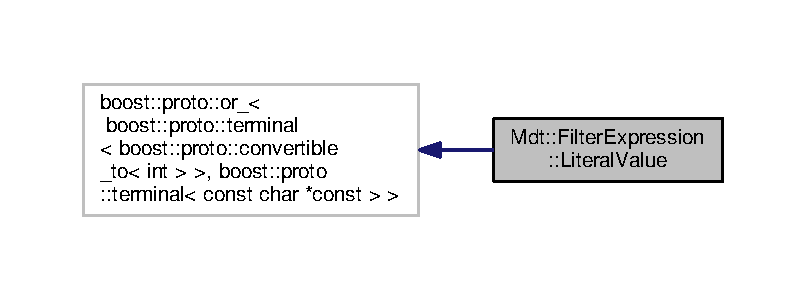
\includegraphics[width=350pt]{struct_mdt_1_1_filter_expression_1_1_literal_value__inherit__graph}
\end{center}
\end{figure}


Collaboration diagram for Mdt\+:\+:Filter\+Expression\+:\+:Literal\+Value\+:
\nopagebreak
\begin{figure}[H]
\begin{center}
\leavevmode
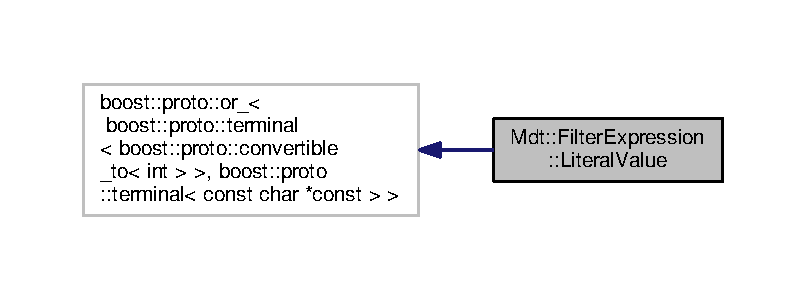
\includegraphics[width=350pt]{struct_mdt_1_1_filter_expression_1_1_literal_value__coll__graph}
\end{center}
\end{figure}


\subsection{Detailed Description}
Literal value grammar. 

Definition at line 31 of file Literal\+Value.\+h.



The documentation for this struct was generated from the following file\+:\begin{DoxyCompactItemize}
\item 
libs/\+Filter\+Expression/src/\+Mdt/\+Filter\+Expression/Literal\+Value.\+h\end{DoxyCompactItemize}

\hypertarget{class_mdt_1_1_error_logger_1_1_logger}{}\section{Mdt\+:\+:Error\+Logger\+:\+:Logger Class Reference}
\label{class_mdt_1_1_error_logger_1_1_logger}\index{Mdt\+::\+Error\+Logger\+::\+Logger@{Mdt\+::\+Error\+Logger\+::\+Logger}}


Helper class to log \hyperlink{class_mdt_1_1_error}{Error} objects.  




{\ttfamily \#include $<$Logger.\+h$>$}



Inherits Q\+Object.

\subsection*{Public Types}
\subsection*{Static Public Member Functions}
\begin{DoxyCompactItemize}
\item 
{\footnotesize template$<$typename T $>$ }\\static T $\ast$ \hyperlink{class_mdt_1_1_error_logger_1_1_logger_ae011d85c251d55660c3f90f21d1ab2a6}{add\+Backend} (\hyperlink{class_mdt_1_1_error_logger_1_1_logger_ab6d6198b43b2bb94cede114ec67b781c}{Execution\+Thread} execution\+Thread)
\begin{DoxyCompactList}\small\item\em Add a logger backend. \end{DoxyCompactList}\item 
static void \hyperlink{class_mdt_1_1_error_logger_1_1_logger_aa06a24a1d521258729ca172465b02040}{log\+Error} (const \hyperlink{class_mdt_1_1_error}{Error} \&error)
\begin{DoxyCompactList}\small\item\em Log given error. \end{DoxyCompactList}\item 
static void \hyperlink{class_mdt_1_1_error_logger_1_1_logger_a3bb1951ee52da826fde82dab52d54c4b}{cleanup} ()
\begin{DoxyCompactList}\small\item\em Cleanup. \end{DoxyCompactList}\end{DoxyCompactItemize}


\subsection{Detailed Description}
Helper class to log \hyperlink{class_mdt_1_1_error}{Error} objects. 

Definition at line 41 of file Logger.\+h.



\subsection{Member Enumeration Documentation}
\index{Mdt\+::\+Error\+Logger\+::\+Logger@{Mdt\+::\+Error\+Logger\+::\+Logger}!Execution\+Thread@{Execution\+Thread}}
\index{Execution\+Thread@{Execution\+Thread}!Mdt\+::\+Error\+Logger\+::\+Logger@{Mdt\+::\+Error\+Logger\+::\+Logger}}
\subsubsection[{\texorpdfstring{Execution\+Thread}{ExecutionThread}}]{\setlength{\rightskip}{0pt plus 5cm}enum {\bf Mdt\+::\+Error\+Logger\+::\+Logger\+::\+Execution\+Thread}}\hypertarget{class_mdt_1_1_error_logger_1_1_logger_ab6d6198b43b2bb94cede114ec67b781c}{}\label{class_mdt_1_1_error_logger_1_1_logger_ab6d6198b43b2bb94cede114ec67b781c}


Execution thread of a backend. 

When adding a backend to the logger, it is possible to choose in which thread it must run. \begin{Desc}
\item[Enumerator]\par
\begin{description}
\index{Execute\+In\+Main\+Thread@{Execute\+In\+Main\+Thread}!Mdt\+::\+Error\+Logger\+::\+Logger@{Mdt\+::\+Error\+Logger\+::\+Logger}}\index{Mdt\+::\+Error\+Logger\+::\+Logger@{Mdt\+::\+Error\+Logger\+::\+Logger}!Execute\+In\+Main\+Thread@{Execute\+In\+Main\+Thread}}\item[{\em 
Execute\+In\+Main\+Thread\hypertarget{class_mdt_1_1_error_logger_1_1_logger_ab6d6198b43b2bb94cede114ec67b781caac54433e68e1f766627c9fcc87f7b818}{}\label{class_mdt_1_1_error_logger_1_1_logger_ab6d6198b43b2bb94cede114ec67b781caac54433e68e1f766627c9fcc87f7b818}
}]The backend will run in the main thread. The Qt\textquotesingle{}s signal/slot is used with a auto connection, so that errors logged using \hyperlink{class_mdt_1_1_error_logger_1_1_logger_aa06a24a1d521258729ca172465b02040}{log\+Error()} will allways call \hyperlink{class_mdt_1_1_error_logger_1_1_backend_acf37cfc576269934ca8ce04e3601058d}{Backend\+::log\+Error()} from the main thread event loop, regardless of the caller thread. \index{Execute\+In\+Separate\+Thread@{Execute\+In\+Separate\+Thread}!Mdt\+::\+Error\+Logger\+::\+Logger@{Mdt\+::\+Error\+Logger\+::\+Logger}}\index{Mdt\+::\+Error\+Logger\+::\+Logger@{Mdt\+::\+Error\+Logger\+::\+Logger}!Execute\+In\+Separate\+Thread@{Execute\+In\+Separate\+Thread}}\item[{\em 
Execute\+In\+Separate\+Thread\hypertarget{class_mdt_1_1_error_logger_1_1_logger_ab6d6198b43b2bb94cede114ec67b781caf7dfdc36418cac0a65cea2cde2a11fd7}{}\label{class_mdt_1_1_error_logger_1_1_logger_ab6d6198b43b2bb94cede114ec67b781caf7dfdc36418cac0a65cea2cde2a11fd7}
}]The backend will run in logger\textquotesingle{}s separate thread. A call to \hyperlink{class_mdt_1_1_error_logger_1_1_logger_aa06a24a1d521258729ca172465b02040}{log\+Error()} will allways just queue the error and return. The logger\textquotesingle{}s separated thread will then call \hyperlink{class_mdt_1_1_error_logger_1_1_backend_acf37cfc576269934ca8ce04e3601058d}{Backend\+::log\+Error()}. \end{description}
\end{Desc}


Definition at line 53 of file Logger.\+h.



\subsection{Member Function Documentation}
\index{Mdt\+::\+Error\+Logger\+::\+Logger@{Mdt\+::\+Error\+Logger\+::\+Logger}!add\+Backend@{add\+Backend}}
\index{add\+Backend@{add\+Backend}!Mdt\+::\+Error\+Logger\+::\+Logger@{Mdt\+::\+Error\+Logger\+::\+Logger}}
\subsubsection[{\texorpdfstring{add\+Backend(\+Execution\+Thread execution\+Thread)}{addBackend(ExecutionThread executionThread)}}]{\setlength{\rightskip}{0pt plus 5cm}template$<$typename T $>$ static T$\ast$ Mdt\+::\+Error\+Logger\+::\+Logger\+::add\+Backend (
\begin{DoxyParamCaption}
\item[{{\bf Execution\+Thread}}]{execution\+Thread}
\end{DoxyParamCaption}
)\hspace{0.3cm}{\ttfamily [inline]}, {\ttfamily [static]}}\hypertarget{class_mdt_1_1_error_logger_1_1_logger_ae011d85c251d55660c3f90f21d1ab2a6}{}\label{class_mdt_1_1_error_logger_1_1_logger_ae011d85c251d55660c3f90f21d1ab2a6}


Add a logger backend. 


\begin{DoxyCode}
\textcolor{keyword}{using} \hyperlink{class_mdt_1_1_error_logger_1_1_logger}{Mdt::ErrorLogger::Logger};

\textcolor{keyword}{auto} backend = Logger::addBackend<FileBackend>(\hyperlink{class_mdt_1_1_error_logger_1_1_logger_ab6d6198b43b2bb94cede114ec67b781caf7dfdc36418cac0a65cea2cde2a11fd7}{Logger::ExecuteInSeparateThread}
      );
backend->setLogFilePath(\textcolor{stringliteral}{"some/path/to/logfile"});
\end{DoxyCode}


A backend of type T is instanciated and added to the list of backends runing on specified {\itshape execution\+Thread} . A pointer to the created backend is returned, so that some setup can be done on the backend. The logger has the ownership of the backend (it will delete it).

Accessing the backend referenced by the returned pointer is only possible\+:
\begin{DoxyItemize}
\item If it runs on separate thread, before any error is logged ( by calling \hyperlink{class_mdt_1_1_error_logger_1_1_logger_aa06a24a1d521258729ca172465b02040}{log\+Error()} )
\item For all cases, before calling \hyperlink{class_mdt_1_1_error_logger_1_1_logger_a3bb1951ee52da826fde82dab52d54c4b}{cleanup()} 
\end{DoxyItemize}

Definition at line 94 of file Logger.\+h.

\index{Mdt\+::\+Error\+Logger\+::\+Logger@{Mdt\+::\+Error\+Logger\+::\+Logger}!cleanup@{cleanup}}
\index{cleanup@{cleanup}!Mdt\+::\+Error\+Logger\+::\+Logger@{Mdt\+::\+Error\+Logger\+::\+Logger}}
\subsubsection[{\texorpdfstring{cleanup()}{cleanup()}}]{\setlength{\rightskip}{0pt plus 5cm}void Mdt\+::\+Error\+Logger\+::\+Logger\+::cleanup (
\begin{DoxyParamCaption}
{}
\end{DoxyParamCaption}
)\hspace{0.3cm}{\ttfamily [static]}}\hypertarget{class_mdt_1_1_error_logger_1_1_logger_a3bb1951ee52da826fde82dab52d54c4b}{}\label{class_mdt_1_1_error_logger_1_1_logger_a3bb1951ee52da826fde82dab52d54c4b}


Cleanup. 

\begin{DoxyNote}{Note}
This function must be called before returning from main(). Not doing so conducts to undefined behaviour. Consider using a \hyperlink{class_mdt_1_1_error_logger_1_1_logger_guard}{Logger\+Guard}. 
\end{DoxyNote}


Definition at line 36 of file Logger.\+cpp.

\index{Mdt\+::\+Error\+Logger\+::\+Logger@{Mdt\+::\+Error\+Logger\+::\+Logger}!log\+Error@{log\+Error}}
\index{log\+Error@{log\+Error}!Mdt\+::\+Error\+Logger\+::\+Logger@{Mdt\+::\+Error\+Logger\+::\+Logger}}
\subsubsection[{\texorpdfstring{log\+Error(const Error \&error)}{logError(const Error &error)}}]{\setlength{\rightskip}{0pt plus 5cm}void Mdt\+::\+Error\+Logger\+::\+Logger\+::log\+Error (
\begin{DoxyParamCaption}
\item[{const {\bf Error} \&}]{error}
\end{DoxyParamCaption}
)\hspace{0.3cm}{\ttfamily [static]}}\hypertarget{class_mdt_1_1_error_logger_1_1_logger_aa06a24a1d521258729ca172465b02040}{}\label{class_mdt_1_1_error_logger_1_1_logger_aa06a24a1d521258729ca172465b02040}


Log given error. 

This function is thread safe

\begin{DoxyPrecond}{Precondition}
{\itshape error} must not be null 
\end{DoxyPrecond}


Definition at line 28 of file Logger.\+cpp.



The documentation for this class was generated from the following files\+:\begin{DoxyCompactItemize}
\item 
libs/\+Error\+\_\+\+Core/src/\+Mdt/\+Error\+Logger/Logger.\+h\item 
libs/\+Error\+\_\+\+Core/src/\+Mdt/\+Error\+Logger/Logger.\+cpp\end{DoxyCompactItemize}

\hypertarget{class_mdt_1_1_error_logger_1_1_logger_guard}{}\section{Mdt\+:\+:Error\+Logger\+:\+:Logger\+Guard Class Reference}
\label{class_mdt_1_1_error_logger_1_1_logger_guard}\index{Mdt\+::\+Error\+Logger\+::\+Logger\+Guard@{Mdt\+::\+Error\+Logger\+::\+Logger\+Guard}}


Scope guard for error \hyperlink{class_mdt_1_1_error_logger_1_1_logger}{Logger}.  




{\ttfamily \#include $<$Logger.\+h$>$}

\subsection*{Public Member Functions}
\begin{DoxyCompactItemize}
\item 
\hyperlink{class_mdt_1_1_error_logger_1_1_logger_guard_a206dae2204438c86ce5fb70470b800e4}{Logger\+Guard} ()
\begin{DoxyCompactList}\small\item\em Constructor. \end{DoxyCompactList}\item 
\hyperlink{class_mdt_1_1_error_logger_1_1_logger_guard_a46942a98dcdf36a9df5857e9114e7466}{$\sim$\+Logger\+Guard} ()
\begin{DoxyCompactList}\small\item\em Destructor. \end{DoxyCompactList}\end{DoxyCompactItemize}


\subsection{Detailed Description}
Scope guard for error \hyperlink{class_mdt_1_1_error_logger_1_1_logger}{Logger}. 

Typical usage\+: 
\begin{DoxyCode}
\textcolor{keywordtype}{int} main()
\{
  \textcolor{keyword}{using} Mdt::Error::Logger;
  \textcolor{keyword}{using} Mdt::Error::LoggerGuard;

  \hyperlink{class_mdt_1_1_error_logger_1_1_logger_guard_a206dae2204438c86ce5fb70470b800e4}{LoggerGuard} loggerGuard;

  \textcolor{comment}{// .. application code}

  \textcolor{comment}{// Here, Logger::cleanup() will be called by loggerGuard.}
\}
\end{DoxyCode}


\begin{DoxyNote}{Note}
When using one of the \hyperlink{namespace_mdt}{Mdt} \hyperlink{class_mdt_1_1_application}{Application}, the error logger is initialized, and logger\textquotesingle{}s cleanup is also called in its destructor.
\end{DoxyNote}
\begin{DoxySeeAlso}{See also}
\hyperlink{class_mdt_1_1_core_application}{Mdt\+::\+Core\+Application} 

\hyperlink{class_mdt_1_1_single_core_application}{Mdt\+::\+Single\+Core\+Application} 

\hyperlink{class_mdt_1_1_application}{Mdt\+::\+Application} 

\hyperlink{class_mdt_1_1_single_application}{Mdt\+::\+Single\+Application} 
\end{DoxySeeAlso}


Definition at line 219 of file Logger.\+h.



\subsection{Constructor \& Destructor Documentation}
\index{Mdt\+::\+Error\+Logger\+::\+Logger\+Guard@{Mdt\+::\+Error\+Logger\+::\+Logger\+Guard}!Logger\+Guard@{Logger\+Guard}}
\index{Logger\+Guard@{Logger\+Guard}!Mdt\+::\+Error\+Logger\+::\+Logger\+Guard@{Mdt\+::\+Error\+Logger\+::\+Logger\+Guard}}
\subsubsection[{\texorpdfstring{Logger\+Guard()}{LoggerGuard()}}]{\setlength{\rightskip}{0pt plus 5cm}Mdt\+::\+Error\+Logger\+::\+Logger\+Guard\+::\+Logger\+Guard (
\begin{DoxyParamCaption}
{}
\end{DoxyParamCaption}
)}\hypertarget{class_mdt_1_1_error_logger_1_1_logger_guard_a206dae2204438c86ce5fb70470b800e4}{}\label{class_mdt_1_1_error_logger_1_1_logger_guard_a206dae2204438c86ce5fb70470b800e4}


Constructor. 



Definition at line 184 of file Logger.\+cpp.

\index{Mdt\+::\+Error\+Logger\+::\+Logger\+Guard@{Mdt\+::\+Error\+Logger\+::\+Logger\+Guard}!````~Logger\+Guard@{$\sim$\+Logger\+Guard}}
\index{````~Logger\+Guard@{$\sim$\+Logger\+Guard}!Mdt\+::\+Error\+Logger\+::\+Logger\+Guard@{Mdt\+::\+Error\+Logger\+::\+Logger\+Guard}}
\subsubsection[{\texorpdfstring{$\sim$\+Logger\+Guard()}{~LoggerGuard()}}]{\setlength{\rightskip}{0pt plus 5cm}Mdt\+::\+Error\+Logger\+::\+Logger\+Guard\+::$\sim$\+Logger\+Guard (
\begin{DoxyParamCaption}
{}
\end{DoxyParamCaption}
)}\hypertarget{class_mdt_1_1_error_logger_1_1_logger_guard_a46942a98dcdf36a9df5857e9114e7466}{}\label{class_mdt_1_1_error_logger_1_1_logger_guard_a46942a98dcdf36a9df5857e9114e7466}


Destructor. 

Will call cleanup on error logger 

Definition at line 188 of file Logger.\+cpp.



The documentation for this class was generated from the following files\+:\begin{DoxyCompactItemize}
\item 
libs/\+Error\+\_\+\+Core/src/\+Mdt/\+Error\+Logger/Logger.\+h\item 
libs/\+Error\+\_\+\+Core/src/\+Mdt/\+Error\+Logger/Logger.\+cpp\end{DoxyCompactItemize}

\hypertarget{class_mdt_1_1_deploy_utils_1_1_objdump_binary_format_parser}{}\section{Mdt\+:\+:Deploy\+Utils\+:\+:Objdump\+Binary\+Format\+Parser Class Reference}
\label{class_mdt_1_1_deploy_utils_1_1_objdump_binary_format_parser}\index{Mdt\+::\+Deploy\+Utils\+::\+Objdump\+Binary\+Format\+Parser@{Mdt\+::\+Deploy\+Utils\+::\+Objdump\+Binary\+Format\+Parser}}


Objdump binary format parser.  




{\ttfamily \#include $<$Objdump\+Binary\+Format\+Parser.\+h$>$}

\subsection*{Public Member Functions}
\begin{DoxyCompactItemize}
\item 
\hyperlink{class_mdt_1_1_deploy_utils_1_1_objdump_binary_format_parser_ab2f0bcb7702627750646fb6efeb50015}{Objdump\+Binary\+Format\+Parser} ()\hypertarget{class_mdt_1_1_deploy_utils_1_1_objdump_binary_format_parser_ab2f0bcb7702627750646fb6efeb50015}{}\label{class_mdt_1_1_deploy_utils_1_1_objdump_binary_format_parser_ab2f0bcb7702627750646fb6efeb50015}

\begin{DoxyCompactList}\small\item\em Constructor. \end{DoxyCompactList}\item 
\hyperlink{class_mdt_1_1_deploy_utils_1_1_objdump_binary_format_parser_a9715218199f46b21e7f217d22e6eed5b}{$\sim$\+Objdump\+Binary\+Format\+Parser} ()\hypertarget{class_mdt_1_1_deploy_utils_1_1_objdump_binary_format_parser_a9715218199f46b21e7f217d22e6eed5b}{}\label{class_mdt_1_1_deploy_utils_1_1_objdump_binary_format_parser_a9715218199f46b21e7f217d22e6eed5b}

\begin{DoxyCompactList}\small\item\em Destructor. \end{DoxyCompactList}\item 
bool \hyperlink{class_mdt_1_1_deploy_utils_1_1_objdump_binary_format_parser_a83e87522f42004c12d61301bbc0f1b3d}{parse} (const Q\+String \&data)\hypertarget{class_mdt_1_1_deploy_utils_1_1_objdump_binary_format_parser_a83e87522f42004c12d61301bbc0f1b3d}{}\label{class_mdt_1_1_deploy_utils_1_1_objdump_binary_format_parser_a83e87522f42004c12d61301bbc0f1b3d}

\begin{DoxyCompactList}\small\item\em Prase the objdump output data. \end{DoxyCompactList}\item 
\hyperlink{namespace_mdt_1_1_deploy_utils_a998c3ae583084b7cac9e9a71b9e1ac32}{Operating\+System} \hyperlink{class_mdt_1_1_deploy_utils_1_1_objdump_binary_format_parser_a694b0f3588b82a98f8e6dc79b0647c53}{operatind\+System} () const 
\begin{DoxyCompactList}\small\item\em Get operating system. \end{DoxyCompactList}\item 
\hyperlink{namespace_mdt_1_1_deploy_utils_aa3c03f55a06150c118902133f9a74b6f}{Processor} \hyperlink{class_mdt_1_1_deploy_utils_1_1_objdump_binary_format_parser_a7348b1d1b12576a2de454dfd162ef41a}{processor} () const 
\begin{DoxyCompactList}\small\item\em Get processor. \end{DoxyCompactList}\end{DoxyCompactItemize}


\subsection{Detailed Description}
Objdump binary format parser. 

Definition at line 41 of file Objdump\+Binary\+Format\+Parser.\+h.



\subsection{Member Function Documentation}
\index{Mdt\+::\+Deploy\+Utils\+::\+Objdump\+Binary\+Format\+Parser@{Mdt\+::\+Deploy\+Utils\+::\+Objdump\+Binary\+Format\+Parser}!operatind\+System@{operatind\+System}}
\index{operatind\+System@{operatind\+System}!Mdt\+::\+Deploy\+Utils\+::\+Objdump\+Binary\+Format\+Parser@{Mdt\+::\+Deploy\+Utils\+::\+Objdump\+Binary\+Format\+Parser}}
\subsubsection[{\texorpdfstring{operatind\+System() const }{operatindSystem() const }}]{\setlength{\rightskip}{0pt plus 5cm}{\bf Operating\+System} Mdt\+::\+Deploy\+Utils\+::\+Objdump\+Binary\+Format\+Parser\+::operatind\+System (
\begin{DoxyParamCaption}
{}
\end{DoxyParamCaption}
) const\hspace{0.3cm}{\ttfamily [inline]}}\hypertarget{class_mdt_1_1_deploy_utils_1_1_objdump_binary_format_parser_a694b0f3588b82a98f8e6dc79b0647c53}{}\label{class_mdt_1_1_deploy_utils_1_1_objdump_binary_format_parser_a694b0f3588b82a98f8e6dc79b0647c53}


Get operating system. 

Return only a valid value after \hyperlink{class_mdt_1_1_deploy_utils_1_1_objdump_binary_format_parser_a83e87522f42004c12d61301bbc0f1b3d}{parse()} succeded 

Definition at line 61 of file Objdump\+Binary\+Format\+Parser.\+h.

\index{Mdt\+::\+Deploy\+Utils\+::\+Objdump\+Binary\+Format\+Parser@{Mdt\+::\+Deploy\+Utils\+::\+Objdump\+Binary\+Format\+Parser}!processor@{processor}}
\index{processor@{processor}!Mdt\+::\+Deploy\+Utils\+::\+Objdump\+Binary\+Format\+Parser@{Mdt\+::\+Deploy\+Utils\+::\+Objdump\+Binary\+Format\+Parser}}
\subsubsection[{\texorpdfstring{processor() const }{processor() const }}]{\setlength{\rightskip}{0pt plus 5cm}{\bf Processor} Mdt\+::\+Deploy\+Utils\+::\+Objdump\+Binary\+Format\+Parser\+::processor (
\begin{DoxyParamCaption}
{}
\end{DoxyParamCaption}
) const\hspace{0.3cm}{\ttfamily [inline]}}\hypertarget{class_mdt_1_1_deploy_utils_1_1_objdump_binary_format_parser_a7348b1d1b12576a2de454dfd162ef41a}{}\label{class_mdt_1_1_deploy_utils_1_1_objdump_binary_format_parser_a7348b1d1b12576a2de454dfd162ef41a}


Get processor. 

Return only a valid value after \hyperlink{class_mdt_1_1_deploy_utils_1_1_objdump_binary_format_parser_a83e87522f42004c12d61301bbc0f1b3d}{parse()} succeded 

Definition at line 70 of file Objdump\+Binary\+Format\+Parser.\+h.



The documentation for this class was generated from the following files\+:\begin{DoxyCompactItemize}
\item 
libs/\+Deploy\+Utils\+\_\+\+Core/src/\+Mdt/\+Deploy\+Utils/Objdump\+Binary\+Format\+Parser.\+h\item 
libs/\+Deploy\+Utils\+\_\+\+Core/src/\+Mdt/\+Deploy\+Utils/Objdump\+Binary\+Format\+Parser.\+cpp\end{DoxyCompactItemize}

\hypertarget{class_mdt_1_1_deploy_utils_1_1_objdump_dependencies_parser}{}\section{Mdt\+:\+:Deploy\+Utils\+:\+:Objdump\+Dependencies\+Parser Class Reference}
\label{class_mdt_1_1_deploy_utils_1_1_objdump_dependencies_parser}\index{Mdt\+::\+Deploy\+Utils\+::\+Objdump\+Dependencies\+Parser@{Mdt\+::\+Deploy\+Utils\+::\+Objdump\+Dependencies\+Parser}}


Objdump dependencies parser.  




{\ttfamily \#include $<$Objdump\+Dependencies\+Parser.\+h$>$}

\subsection*{Public Member Functions}
\begin{DoxyCompactItemize}
\item 
\hyperlink{class_mdt_1_1_deploy_utils_1_1_objdump_dependencies_parser_ae543b682413540d2b3ffb472588a939b}{Objdump\+Dependencies\+Parser} ()\hypertarget{class_mdt_1_1_deploy_utils_1_1_objdump_dependencies_parser_ae543b682413540d2b3ffb472588a939b}{}\label{class_mdt_1_1_deploy_utils_1_1_objdump_dependencies_parser_ae543b682413540d2b3ffb472588a939b}

\begin{DoxyCompactList}\small\item\em Constructor. \end{DoxyCompactList}\item 
\hyperlink{class_mdt_1_1_deploy_utils_1_1_objdump_dependencies_parser_a25d5d1b986d8fd8813a400f43e8293b0}{$\sim$\+Objdump\+Dependencies\+Parser} ()\hypertarget{class_mdt_1_1_deploy_utils_1_1_objdump_dependencies_parser_a25d5d1b986d8fd8813a400f43e8293b0}{}\label{class_mdt_1_1_deploy_utils_1_1_objdump_dependencies_parser_a25d5d1b986d8fd8813a400f43e8293b0}

\begin{DoxyCompactList}\small\item\em Destructor. \end{DoxyCompactList}\item 
bool \hyperlink{class_mdt_1_1_deploy_utils_1_1_objdump_dependencies_parser_af70d3b3ccf5bf277e3b294f12c167819}{parse} (const Q\+String \&data)\hypertarget{class_mdt_1_1_deploy_utils_1_1_objdump_dependencies_parser_af70d3b3ccf5bf277e3b294f12c167819}{}\label{class_mdt_1_1_deploy_utils_1_1_objdump_dependencies_parser_af70d3b3ccf5bf277e3b294f12c167819}

\begin{DoxyCompactList}\small\item\em Prase the objdump output data. \end{DoxyCompactList}\item 
Mdt\+::\+Plain\+Text\+::\+String\+Record\+List \hyperlink{class_mdt_1_1_deploy_utils_1_1_objdump_dependencies_parser_a772af6ac8d2b7e5dbdc354aeb404db0d}{raw\+Dependencies} () const \hypertarget{class_mdt_1_1_deploy_utils_1_1_objdump_dependencies_parser_a772af6ac8d2b7e5dbdc354aeb404db0d}{}\label{class_mdt_1_1_deploy_utils_1_1_objdump_dependencies_parser_a772af6ac8d2b7e5dbdc354aeb404db0d}

\begin{DoxyCompactList}\small\item\em Get parsed dependencies. \end{DoxyCompactList}\end{DoxyCompactItemize}


\subsection{Detailed Description}
Objdump dependencies parser. 

Definition at line 40 of file Objdump\+Dependencies\+Parser.\+h.



The documentation for this class was generated from the following files\+:\begin{DoxyCompactItemize}
\item 
libs/\+Deploy\+Utils\+\_\+\+Core/src/\+Mdt/\+Deploy\+Utils/Objdump\+Dependencies\+Parser.\+h\item 
libs/\+Deploy\+Utils\+\_\+\+Core/src/\+Mdt/\+Deploy\+Utils/Objdump\+Dependencies\+Parser.\+cpp\end{DoxyCompactItemize}

\hypertarget{class_mdt_1_1_deploy_utils_1_1_objdump_wrapper}{}\section{Mdt\+:\+:Deploy\+Utils\+:\+:Objdump\+Wrapper Class Reference}
\label{class_mdt_1_1_deploy_utils_1_1_objdump_wrapper}\index{Mdt\+::\+Deploy\+Utils\+::\+Objdump\+Wrapper@{Mdt\+::\+Deploy\+Utils\+::\+Objdump\+Wrapper}}


Wrapps a objdump executable.  




{\ttfamily \#include $<$Objdump\+Wrapper.\+h$>$}



Inheritance diagram for Mdt\+:\+:Deploy\+Utils\+:\+:Objdump\+Wrapper\+:\nopagebreak
\begin{figure}[H]
\begin{center}
\leavevmode
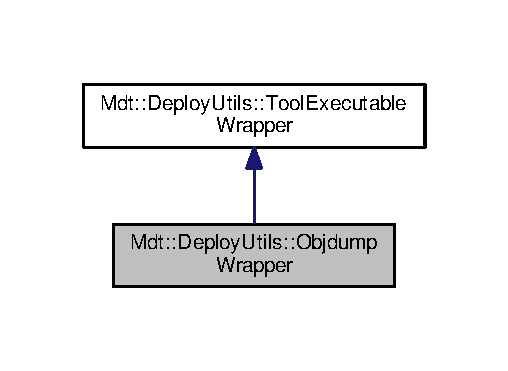
\includegraphics[width=244pt]{class_mdt_1_1_deploy_utils_1_1_objdump_wrapper__inherit__graph}
\end{center}
\end{figure}


Collaboration diagram for Mdt\+:\+:Deploy\+Utils\+:\+:Objdump\+Wrapper\+:\nopagebreak
\begin{figure}[H]
\begin{center}
\leavevmode
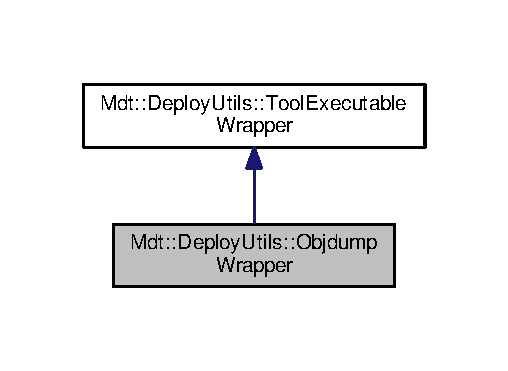
\includegraphics[width=244pt]{class_mdt_1_1_deploy_utils_1_1_objdump_wrapper__coll__graph}
\end{center}
\end{figure}
\subsection*{Public Member Functions}
\begin{DoxyCompactItemize}
\item 
\hyperlink{class_mdt_1_1_deploy_utils_1_1_objdump_wrapper_a6f042e9d1554f14fcc320c2efef16ffa}{Objdump\+Wrapper} (Q\+Object $\ast$parent=nullptr)\hypertarget{class_mdt_1_1_deploy_utils_1_1_objdump_wrapper_a6f042e9d1554f14fcc320c2efef16ffa}{}\label{class_mdt_1_1_deploy_utils_1_1_objdump_wrapper_a6f042e9d1554f14fcc320c2efef16ffa}

\begin{DoxyCompactList}\small\item\em Constructor. \end{DoxyCompactList}\item 
bool \hyperlink{class_mdt_1_1_deploy_utils_1_1_objdump_wrapper_ab97db66a2a9ad2db9932a7c833c11cd1}{exec\+Find\+Dependencies} (const Q\+String \&binary\+File\+Path)
\begin{DoxyCompactList}\small\item\em Execute the command to find dependencies. \end{DoxyCompactList}\item 
bool \hyperlink{class_mdt_1_1_deploy_utils_1_1_objdump_wrapper_a38237494f7027dec851514c7f7179278}{exec\+Read\+Format} (const Q\+String \&binary\+File\+Path)
\begin{DoxyCompactList}\small\item\em Execute the command to read format. \end{DoxyCompactList}\item 
Q\+String \hyperlink{class_mdt_1_1_deploy_utils_1_1_objdump_wrapper_a515708420d15527141d19c365d3f1bd6}{find\+Objdump} ()
\begin{DoxyCompactList}\small\item\em Find objdump executable. \end{DoxyCompactList}\end{DoxyCompactItemize}
\subsection*{Additional Inherited Members}


\subsection{Detailed Description}
Wrapps a objdump executable. 

Definition at line 32 of file Objdump\+Wrapper.\+h.



\subsection{Member Function Documentation}
\index{Mdt\+::\+Deploy\+Utils\+::\+Objdump\+Wrapper@{Mdt\+::\+Deploy\+Utils\+::\+Objdump\+Wrapper}!exec\+Find\+Dependencies@{exec\+Find\+Dependencies}}
\index{exec\+Find\+Dependencies@{exec\+Find\+Dependencies}!Mdt\+::\+Deploy\+Utils\+::\+Objdump\+Wrapper@{Mdt\+::\+Deploy\+Utils\+::\+Objdump\+Wrapper}}
\subsubsection[{\texorpdfstring{exec\+Find\+Dependencies(const Q\+String \&binary\+File\+Path)}{execFindDependencies(const QString &binaryFilePath)}}]{\setlength{\rightskip}{0pt plus 5cm}bool Mdt\+::\+Deploy\+Utils\+::\+Objdump\+Wrapper\+::exec\+Find\+Dependencies (
\begin{DoxyParamCaption}
\item[{const Q\+String \&}]{binary\+File\+Path}
\end{DoxyParamCaption}
)}\hypertarget{class_mdt_1_1_deploy_utils_1_1_objdump_wrapper_ab97db66a2a9ad2db9932a7c833c11cd1}{}\label{class_mdt_1_1_deploy_utils_1_1_objdump_wrapper_ab97db66a2a9ad2db9932a7c833c11cd1}


Execute the command to find dependencies. 


\begin{DoxyParams}{Parameters}
{\em binary\+File\+Path} & Path to a executable or a library \\
\hline
\end{DoxyParams}


Definition at line 36 of file Objdump\+Wrapper.\+cpp.

\index{Mdt\+::\+Deploy\+Utils\+::\+Objdump\+Wrapper@{Mdt\+::\+Deploy\+Utils\+::\+Objdump\+Wrapper}!exec\+Read\+Format@{exec\+Read\+Format}}
\index{exec\+Read\+Format@{exec\+Read\+Format}!Mdt\+::\+Deploy\+Utils\+::\+Objdump\+Wrapper@{Mdt\+::\+Deploy\+Utils\+::\+Objdump\+Wrapper}}
\subsubsection[{\texorpdfstring{exec\+Read\+Format(const Q\+String \&binary\+File\+Path)}{execReadFormat(const QString &binaryFilePath)}}]{\setlength{\rightskip}{0pt plus 5cm}bool Mdt\+::\+Deploy\+Utils\+::\+Objdump\+Wrapper\+::exec\+Read\+Format (
\begin{DoxyParamCaption}
\item[{const Q\+String \&}]{binary\+File\+Path}
\end{DoxyParamCaption}
)}\hypertarget{class_mdt_1_1_deploy_utils_1_1_objdump_wrapper_a38237494f7027dec851514c7f7179278}{}\label{class_mdt_1_1_deploy_utils_1_1_objdump_wrapper_a38237494f7027dec851514c7f7179278}


Execute the command to read format. 


\begin{DoxyParams}{Parameters}
{\em binary\+File\+Path} & Path to a executable or a library \\
\hline
\end{DoxyParams}


Definition at line 41 of file Objdump\+Wrapper.\+cpp.

\index{Mdt\+::\+Deploy\+Utils\+::\+Objdump\+Wrapper@{Mdt\+::\+Deploy\+Utils\+::\+Objdump\+Wrapper}!find\+Objdump@{find\+Objdump}}
\index{find\+Objdump@{find\+Objdump}!Mdt\+::\+Deploy\+Utils\+::\+Objdump\+Wrapper@{Mdt\+::\+Deploy\+Utils\+::\+Objdump\+Wrapper}}
\subsubsection[{\texorpdfstring{find\+Objdump()}{findObjdump()}}]{\setlength{\rightskip}{0pt plus 5cm}Q\+String Mdt\+::\+Deploy\+Utils\+::\+Objdump\+Wrapper\+::find\+Objdump (
\begin{DoxyParamCaption}
{}
\end{DoxyParamCaption}
)}\hypertarget{class_mdt_1_1_deploy_utils_1_1_objdump_wrapper_a515708420d15527141d19c365d3f1bd6}{}\label{class_mdt_1_1_deploy_utils_1_1_objdump_wrapper_a515708420d15527141d19c365d3f1bd6}


Find objdump executable. 

\begin{DoxyNote}{Note}
This method is called automatically by find$\ast$() methods. 
\end{DoxyNote}


Definition at line 46 of file Objdump\+Wrapper.\+cpp.



The documentation for this class was generated from the following files\+:\begin{DoxyCompactItemize}
\item 
libs/\+Deploy\+Utils\+\_\+\+Core/src/\+Mdt/\+Deploy\+Utils/Objdump\+Wrapper.\+h\item 
libs/\+Deploy\+Utils\+\_\+\+Core/src/\+Mdt/\+Deploy\+Utils/Objdump\+Wrapper.\+cpp\end{DoxyCompactItemize}

\hypertarget{class_mdt_1_1_deploy_utils_1_1_path_list}{}\section{Mdt\+:\+:Deploy\+Utils\+:\+:Path\+List Class Reference}
\label{class_mdt_1_1_deploy_utils_1_1_path_list}\index{Mdt\+::\+Deploy\+Utils\+::\+Path\+List@{Mdt\+::\+Deploy\+Utils\+::\+Path\+List}}


\hyperlink{class_mdt_1_1_deploy_utils_1_1_path_list}{Path\+List} contains a list of paths.  




{\ttfamily \#include $<$Path\+List.\+h$>$}

\subsection*{Public Types}
\begin{DoxyCompactItemize}
\item 
using \hyperlink{class_mdt_1_1_deploy_utils_1_1_path_list_a2666c4c9348c4f7a28014d4de9599717}{const\+\_\+iterator} = Q\+String\+List\+::const\+\_\+iterator
\begin{DoxyCompactList}\small\item\em S\+T\+L-\/style const iterator. \end{DoxyCompactList}\end{DoxyCompactItemize}
\subsection*{Public Member Functions}
\begin{DoxyCompactItemize}
\item 
\hyperlink{class_mdt_1_1_deploy_utils_1_1_path_list_a4a415acb1aa87350536e9e34980ed7fe}{Path\+List} ()=default
\begin{DoxyCompactList}\small\item\em Construct a empty path list. \end{DoxyCompactList}\item 
\hyperlink{class_mdt_1_1_deploy_utils_1_1_path_list_adc70e99b4aabb7edd3c6ad03a15117a8}{Path\+List} (std\+::initializer\+\_\+list$<$ Q\+String $>$ list)
\begin{DoxyCompactList}\small\item\em Construct a path list from {\itshape list}. \end{DoxyCompactList}\item 
\hyperlink{class_mdt_1_1_deploy_utils_1_1_path_list_a904588c5a1ad74269af5418749e6f8fc}{Path\+List} (const \hyperlink{class_mdt_1_1_deploy_utils_1_1_path_list}{Path\+List} \&)=default
\begin{DoxyCompactList}\small\item\em Copy construct a path list from a other. \end{DoxyCompactList}\item 
\hyperlink{class_mdt_1_1_deploy_utils_1_1_path_list}{Path\+List} \& \hyperlink{class_mdt_1_1_deploy_utils_1_1_path_list_a5be033c921bce08dff33e25122ea3def}{operator=} (const \hyperlink{class_mdt_1_1_deploy_utils_1_1_path_list}{Path\+List} \&)=default
\begin{DoxyCompactList}\small\item\em Assign a path list to this one by copy. \end{DoxyCompactList}\item 
\hyperlink{class_mdt_1_1_deploy_utils_1_1_path_list_aa18f629ded1d797c13d61165b8749bf6}{Path\+List} (\hyperlink{class_mdt_1_1_deploy_utils_1_1_path_list}{Path\+List} \&\&)=default
\begin{DoxyCompactList}\small\item\em Move construct a path list from a other. \end{DoxyCompactList}\item 
\hyperlink{class_mdt_1_1_deploy_utils_1_1_path_list}{Path\+List} \& \hyperlink{class_mdt_1_1_deploy_utils_1_1_path_list_a8f96ea72207a6a869edeff57dbeed43a}{operator=} (\hyperlink{class_mdt_1_1_deploy_utils_1_1_path_list}{Path\+List} \&\&)=default
\begin{DoxyCompactList}\small\item\em Assign a path list to this one by move. \end{DoxyCompactList}\item 
void \hyperlink{class_mdt_1_1_deploy_utils_1_1_path_list_a2d8d99897e5a693e761f6df4523b115c}{append\+Path} (const Q\+String \&path)
\begin{DoxyCompactList}\small\item\em Add a path to the end of this list. \end{DoxyCompactList}\item 
void \hyperlink{class_mdt_1_1_deploy_utils_1_1_path_list_a1d83d10599fac6d015a6779153364ab3}{append\+Path\+List} (const \hyperlink{class_mdt_1_1_deploy_utils_1_1_path_list}{Path\+List} \&path\+List)
\begin{DoxyCompactList}\small\item\em Add a path list to the end of this list. \end{DoxyCompactList}\item 
void \hyperlink{class_mdt_1_1_deploy_utils_1_1_path_list_a3fcd8dbdb27b4ead271623a46fa81b38}{prepend\+Path} (const Q\+String \&path)
\begin{DoxyCompactList}\small\item\em Add a path to the beginning of this list. \end{DoxyCompactList}\item 
void \hyperlink{class_mdt_1_1_deploy_utils_1_1_path_list_a681de54da92349f89f1df37c876e0c67}{prepend\+Path\+List} (const \hyperlink{class_mdt_1_1_deploy_utils_1_1_path_list}{Path\+List} \&path\+List)
\begin{DoxyCompactList}\small\item\em Add a path list to the beginning of this list. \end{DoxyCompactList}\item 
void \hyperlink{class_mdt_1_1_deploy_utils_1_1_path_list_a341e4b7de4f7c6ed11769bd4449aa013}{clear} ()
\begin{DoxyCompactList}\small\item\em Clear this path list. \end{DoxyCompactList}\item 
Q\+String\+List \hyperlink{class_mdt_1_1_deploy_utils_1_1_path_list_afd40c0f5d21c285bb5f1778a8832167e}{to\+String\+List} () const 
\begin{DoxyCompactList}\small\item\em Get a list of strings for this list. \end{DoxyCompactList}\item 
bool \hyperlink{class_mdt_1_1_deploy_utils_1_1_path_list_ae2b68179e5536ee2bc063b133f88bb4a}{is\+Empty} () const 
\begin{DoxyCompactList}\small\item\em Check if this path list is empty. \end{DoxyCompactList}\item 
\hyperlink{class_mdt_1_1_deploy_utils_1_1_path_list_a2666c4c9348c4f7a28014d4de9599717}{const\+\_\+iterator} \hyperlink{class_mdt_1_1_deploy_utils_1_1_path_list_a13c645c41b4492ab0d10b887cb77e739}{begin} () const 
\begin{DoxyCompactList}\small\item\em Returns a const S\+T\+L-\/style iterator pointing to the first item in the list. \end{DoxyCompactList}\item 
\hyperlink{class_mdt_1_1_deploy_utils_1_1_path_list_a2666c4c9348c4f7a28014d4de9599717}{const\+\_\+iterator} \hyperlink{class_mdt_1_1_deploy_utils_1_1_path_list_a980da2988f38bf64bf76f6b61b572582}{cbegin} () const 
\begin{DoxyCompactList}\small\item\em Returns a const S\+T\+L-\/style iterator pointing to the first item in the list. \end{DoxyCompactList}\item 
\hyperlink{class_mdt_1_1_deploy_utils_1_1_path_list_a2666c4c9348c4f7a28014d4de9599717}{const\+\_\+iterator} \hyperlink{class_mdt_1_1_deploy_utils_1_1_path_list_ab65fbf7392d22bf249583ff1aefd3f78}{end} () const 
\begin{DoxyCompactList}\small\item\em Returns a const S\+T\+L-\/style iterator pointing to the last item in the list. \end{DoxyCompactList}\item 
\hyperlink{class_mdt_1_1_deploy_utils_1_1_path_list_a2666c4c9348c4f7a28014d4de9599717}{const\+\_\+iterator} \hyperlink{class_mdt_1_1_deploy_utils_1_1_path_list_a0a36320111aac2c79060dbe778286f54}{cend} () const 
\begin{DoxyCompactList}\small\item\em Returns a const S\+T\+L-\/style iterator pointing to the last item in the list. \end{DoxyCompactList}\end{DoxyCompactItemize}
\subsection*{Static Public Member Functions}
\begin{DoxyCompactItemize}
\item 
static \hyperlink{class_mdt_1_1_deploy_utils_1_1_path_list}{Path\+List} \hyperlink{class_mdt_1_1_deploy_utils_1_1_path_list_aa21f8eef32f3c07d2c54c949a219d7b7}{from\+String\+List} (const Q\+String\+List \&paths)
\begin{DoxyCompactList}\small\item\em Get a path list from a string list. \end{DoxyCompactList}\item 
static \hyperlink{class_mdt_1_1_deploy_utils_1_1_path_list}{Path\+List} \hyperlink{class_mdt_1_1_deploy_utils_1_1_path_list_a71377c7947695d47b9ed88e1ace136d8}{get\+System\+Executable\+Path\+List} ()
\begin{DoxyCompactList}\small\item\em Get a list of system executable paths. \end{DoxyCompactList}\item 
static \hyperlink{class_mdt_1_1_deploy_utils_1_1_path_list}{Path\+List} \hyperlink{class_mdt_1_1_deploy_utils_1_1_path_list_a50b46470e23ed409806563b3a49655e4}{get\+System\+Library\+Path\+List} ()
\begin{DoxyCompactList}\small\item\em Get a list of system library paths. \end{DoxyCompactList}\item 
static \hyperlink{class_mdt_1_1_deploy_utils_1_1_path_list}{Path\+List} \hyperlink{class_mdt_1_1_deploy_utils_1_1_path_list_aaad86a05cd05cd43a059ce4faae98fb2}{get\+System\+Library\+Known\+Path\+List\+Linux} ()
\begin{DoxyCompactList}\small\item\em Get a list of system library paths for Linux. \end{DoxyCompactList}\item 
static \hyperlink{class_mdt_1_1_deploy_utils_1_1_path_list}{Path\+List} \hyperlink{class_mdt_1_1_deploy_utils_1_1_path_list_a94b801e76dc61dac792299af2acf1bd5}{get\+System\+Library\+Known\+Path\+List\+Windows} ()
\begin{DoxyCompactList}\small\item\em Get a list of system library paths for Windows. \end{DoxyCompactList}\end{DoxyCompactItemize}


\subsection{Detailed Description}
\hyperlink{class_mdt_1_1_deploy_utils_1_1_path_list}{Path\+List} contains a list of paths. 

Definition at line 33 of file Path\+List.\+h.



\subsection{Member Typedef Documentation}
\index{Mdt\+::\+Deploy\+Utils\+::\+Path\+List@{Mdt\+::\+Deploy\+Utils\+::\+Path\+List}!const\+\_\+iterator@{const\+\_\+iterator}}
\index{const\+\_\+iterator@{const\+\_\+iterator}!Mdt\+::\+Deploy\+Utils\+::\+Path\+List@{Mdt\+::\+Deploy\+Utils\+::\+Path\+List}}
\subsubsection[{\texorpdfstring{const\+\_\+iterator}{const_iterator}}]{\setlength{\rightskip}{0pt plus 5cm}using {\bf Mdt\+::\+Deploy\+Utils\+::\+Path\+List\+::const\+\_\+iterator} =  Q\+String\+List\+::const\+\_\+iterator}\hypertarget{class_mdt_1_1_deploy_utils_1_1_path_list_a2666c4c9348c4f7a28014d4de9599717}{}\label{class_mdt_1_1_deploy_utils_1_1_path_list_a2666c4c9348c4f7a28014d4de9599717}


S\+T\+L-\/style const iterator. 



Definition at line 39 of file Path\+List.\+h.



\subsection{Constructor \& Destructor Documentation}
\index{Mdt\+::\+Deploy\+Utils\+::\+Path\+List@{Mdt\+::\+Deploy\+Utils\+::\+Path\+List}!Path\+List@{Path\+List}}
\index{Path\+List@{Path\+List}!Mdt\+::\+Deploy\+Utils\+::\+Path\+List@{Mdt\+::\+Deploy\+Utils\+::\+Path\+List}}
\subsubsection[{\texorpdfstring{Path\+List()=default}{PathList()=default}}]{\setlength{\rightskip}{0pt plus 5cm}Mdt\+::\+Deploy\+Utils\+::\+Path\+List\+::\+Path\+List (
\begin{DoxyParamCaption}
{}
\end{DoxyParamCaption}
)\hspace{0.3cm}{\ttfamily [default]}}\hypertarget{class_mdt_1_1_deploy_utils_1_1_path_list_a4a415acb1aa87350536e9e34980ed7fe}{}\label{class_mdt_1_1_deploy_utils_1_1_path_list_a4a415acb1aa87350536e9e34980ed7fe}


Construct a empty path list. 

\index{Mdt\+::\+Deploy\+Utils\+::\+Path\+List@{Mdt\+::\+Deploy\+Utils\+::\+Path\+List}!Path\+List@{Path\+List}}
\index{Path\+List@{Path\+List}!Mdt\+::\+Deploy\+Utils\+::\+Path\+List@{Mdt\+::\+Deploy\+Utils\+::\+Path\+List}}
\subsubsection[{\texorpdfstring{Path\+List(std\+::initializer\+\_\+list$<$ Q\+String $>$ list)}{PathList(std::initializer_list< QString > list)}}]{\setlength{\rightskip}{0pt plus 5cm}Mdt\+::\+Deploy\+Utils\+::\+Path\+List\+::\+Path\+List (
\begin{DoxyParamCaption}
\item[{std\+::initializer\+\_\+list$<$ Q\+String $>$}]{list}
\end{DoxyParamCaption}
)\hspace{0.3cm}{\ttfamily [inline]}}\hypertarget{class_mdt_1_1_deploy_utils_1_1_path_list_adc70e99b4aabb7edd3c6ad03a15117a8}{}\label{class_mdt_1_1_deploy_utils_1_1_path_list_adc70e99b4aabb7edd3c6ad03a15117a8}


Construct a path list from {\itshape list}. 



Definition at line 47 of file Path\+List.\+h.

\index{Mdt\+::\+Deploy\+Utils\+::\+Path\+List@{Mdt\+::\+Deploy\+Utils\+::\+Path\+List}!Path\+List@{Path\+List}}
\index{Path\+List@{Path\+List}!Mdt\+::\+Deploy\+Utils\+::\+Path\+List@{Mdt\+::\+Deploy\+Utils\+::\+Path\+List}}
\subsubsection[{\texorpdfstring{Path\+List(const Path\+List \&)=default}{PathList(const PathList &)=default}}]{\setlength{\rightskip}{0pt plus 5cm}Mdt\+::\+Deploy\+Utils\+::\+Path\+List\+::\+Path\+List (
\begin{DoxyParamCaption}
\item[{const {\bf Path\+List} \&}]{}
\end{DoxyParamCaption}
)\hspace{0.3cm}{\ttfamily [default]}}\hypertarget{class_mdt_1_1_deploy_utils_1_1_path_list_a904588c5a1ad74269af5418749e6f8fc}{}\label{class_mdt_1_1_deploy_utils_1_1_path_list_a904588c5a1ad74269af5418749e6f8fc}


Copy construct a path list from a other. 

\index{Mdt\+::\+Deploy\+Utils\+::\+Path\+List@{Mdt\+::\+Deploy\+Utils\+::\+Path\+List}!Path\+List@{Path\+List}}
\index{Path\+List@{Path\+List}!Mdt\+::\+Deploy\+Utils\+::\+Path\+List@{Mdt\+::\+Deploy\+Utils\+::\+Path\+List}}
\subsubsection[{\texorpdfstring{Path\+List(\+Path\+List \&\&)=default}{PathList(PathList &&)=default}}]{\setlength{\rightskip}{0pt plus 5cm}Mdt\+::\+Deploy\+Utils\+::\+Path\+List\+::\+Path\+List (
\begin{DoxyParamCaption}
\item[{{\bf Path\+List} \&\&}]{}
\end{DoxyParamCaption}
)\hspace{0.3cm}{\ttfamily [default]}}\hypertarget{class_mdt_1_1_deploy_utils_1_1_path_list_aa18f629ded1d797c13d61165b8749bf6}{}\label{class_mdt_1_1_deploy_utils_1_1_path_list_aa18f629ded1d797c13d61165b8749bf6}


Move construct a path list from a other. 



\subsection{Member Function Documentation}
\index{Mdt\+::\+Deploy\+Utils\+::\+Path\+List@{Mdt\+::\+Deploy\+Utils\+::\+Path\+List}!append\+Path@{append\+Path}}
\index{append\+Path@{append\+Path}!Mdt\+::\+Deploy\+Utils\+::\+Path\+List@{Mdt\+::\+Deploy\+Utils\+::\+Path\+List}}
\subsubsection[{\texorpdfstring{append\+Path(const Q\+String \&path)}{appendPath(const QString &path)}}]{\setlength{\rightskip}{0pt plus 5cm}void Mdt\+::\+Deploy\+Utils\+::\+Path\+List\+::append\+Path (
\begin{DoxyParamCaption}
\item[{const Q\+String \&}]{path}
\end{DoxyParamCaption}
)}\hypertarget{class_mdt_1_1_deploy_utils_1_1_path_list_a2d8d99897e5a693e761f6df4523b115c}{}\label{class_mdt_1_1_deploy_utils_1_1_path_list_a2d8d99897e5a693e761f6df4523b115c}


Add a path to the end of this list. 

If {\itshape path} allready exists in this list, it will be moved to the end.

\begin{DoxyPrecond}{Precondition}
{\itshape path} must not be a empty string 
\end{DoxyPrecond}


Definition at line 33 of file Path\+List.\+cpp.

\index{Mdt\+::\+Deploy\+Utils\+::\+Path\+List@{Mdt\+::\+Deploy\+Utils\+::\+Path\+List}!append\+Path\+List@{append\+Path\+List}}
\index{append\+Path\+List@{append\+Path\+List}!Mdt\+::\+Deploy\+Utils\+::\+Path\+List@{Mdt\+::\+Deploy\+Utils\+::\+Path\+List}}
\subsubsection[{\texorpdfstring{append\+Path\+List(const Path\+List \&path\+List)}{appendPathList(const PathList &pathList)}}]{\setlength{\rightskip}{0pt plus 5cm}void Mdt\+::\+Deploy\+Utils\+::\+Path\+List\+::append\+Path\+List (
\begin{DoxyParamCaption}
\item[{const {\bf Path\+List} \&}]{path\+List}
\end{DoxyParamCaption}
)}\hypertarget{class_mdt_1_1_deploy_utils_1_1_path_list_a1d83d10599fac6d015a6779153364ab3}{}\label{class_mdt_1_1_deploy_utils_1_1_path_list_a1d83d10599fac6d015a6779153364ab3}


Add a path list to the end of this list. 

If a path in {\itshape path\+List} allready exists in this list, it will be moved to the end.

If {\itshape path\+List} contains a empty path, it will not be added to this list. 

Definition at line 41 of file Path\+List.\+cpp.

\index{Mdt\+::\+Deploy\+Utils\+::\+Path\+List@{Mdt\+::\+Deploy\+Utils\+::\+Path\+List}!begin@{begin}}
\index{begin@{begin}!Mdt\+::\+Deploy\+Utils\+::\+Path\+List@{Mdt\+::\+Deploy\+Utils\+::\+Path\+List}}
\subsubsection[{\texorpdfstring{begin() const }{begin() const }}]{\setlength{\rightskip}{0pt plus 5cm}{\bf const\+\_\+iterator} Mdt\+::\+Deploy\+Utils\+::\+Path\+List\+::begin (
\begin{DoxyParamCaption}
{}
\end{DoxyParamCaption}
) const\hspace{0.3cm}{\ttfamily [inline]}}\hypertarget{class_mdt_1_1_deploy_utils_1_1_path_list_a13c645c41b4492ab0d10b887cb77e739}{}\label{class_mdt_1_1_deploy_utils_1_1_path_list_a13c645c41b4492ab0d10b887cb77e739}


Returns a const S\+T\+L-\/style iterator pointing to the first item in the list. 



Definition at line 133 of file Path\+List.\+h.

\index{Mdt\+::\+Deploy\+Utils\+::\+Path\+List@{Mdt\+::\+Deploy\+Utils\+::\+Path\+List}!cbegin@{cbegin}}
\index{cbegin@{cbegin}!Mdt\+::\+Deploy\+Utils\+::\+Path\+List@{Mdt\+::\+Deploy\+Utils\+::\+Path\+List}}
\subsubsection[{\texorpdfstring{cbegin() const }{cbegin() const }}]{\setlength{\rightskip}{0pt plus 5cm}{\bf const\+\_\+iterator} Mdt\+::\+Deploy\+Utils\+::\+Path\+List\+::cbegin (
\begin{DoxyParamCaption}
{}
\end{DoxyParamCaption}
) const\hspace{0.3cm}{\ttfamily [inline]}}\hypertarget{class_mdt_1_1_deploy_utils_1_1_path_list_a980da2988f38bf64bf76f6b61b572582}{}\label{class_mdt_1_1_deploy_utils_1_1_path_list_a980da2988f38bf64bf76f6b61b572582}


Returns a const S\+T\+L-\/style iterator pointing to the first item in the list. 



Definition at line 140 of file Path\+List.\+h.

\index{Mdt\+::\+Deploy\+Utils\+::\+Path\+List@{Mdt\+::\+Deploy\+Utils\+::\+Path\+List}!cend@{cend}}
\index{cend@{cend}!Mdt\+::\+Deploy\+Utils\+::\+Path\+List@{Mdt\+::\+Deploy\+Utils\+::\+Path\+List}}
\subsubsection[{\texorpdfstring{cend() const }{cend() const }}]{\setlength{\rightskip}{0pt plus 5cm}{\bf const\+\_\+iterator} Mdt\+::\+Deploy\+Utils\+::\+Path\+List\+::cend (
\begin{DoxyParamCaption}
{}
\end{DoxyParamCaption}
) const\hspace{0.3cm}{\ttfamily [inline]}}\hypertarget{class_mdt_1_1_deploy_utils_1_1_path_list_a0a36320111aac2c79060dbe778286f54}{}\label{class_mdt_1_1_deploy_utils_1_1_path_list_a0a36320111aac2c79060dbe778286f54}


Returns a const S\+T\+L-\/style iterator pointing to the last item in the list. 



Definition at line 154 of file Path\+List.\+h.

\index{Mdt\+::\+Deploy\+Utils\+::\+Path\+List@{Mdt\+::\+Deploy\+Utils\+::\+Path\+List}!clear@{clear}}
\index{clear@{clear}!Mdt\+::\+Deploy\+Utils\+::\+Path\+List@{Mdt\+::\+Deploy\+Utils\+::\+Path\+List}}
\subsubsection[{\texorpdfstring{clear()}{clear()}}]{\setlength{\rightskip}{0pt plus 5cm}void Mdt\+::\+Deploy\+Utils\+::\+Path\+List\+::clear (
\begin{DoxyParamCaption}
{}
\end{DoxyParamCaption}
)}\hypertarget{class_mdt_1_1_deploy_utils_1_1_path_list_a341e4b7de4f7c6ed11769bd4449aa013}{}\label{class_mdt_1_1_deploy_utils_1_1_path_list_a341e4b7de4f7c6ed11769bd4449aa013}


Clear this path list. 



Definition at line 70 of file Path\+List.\+cpp.

\index{Mdt\+::\+Deploy\+Utils\+::\+Path\+List@{Mdt\+::\+Deploy\+Utils\+::\+Path\+List}!end@{end}}
\index{end@{end}!Mdt\+::\+Deploy\+Utils\+::\+Path\+List@{Mdt\+::\+Deploy\+Utils\+::\+Path\+List}}
\subsubsection[{\texorpdfstring{end() const }{end() const }}]{\setlength{\rightskip}{0pt plus 5cm}{\bf const\+\_\+iterator} Mdt\+::\+Deploy\+Utils\+::\+Path\+List\+::end (
\begin{DoxyParamCaption}
{}
\end{DoxyParamCaption}
) const\hspace{0.3cm}{\ttfamily [inline]}}\hypertarget{class_mdt_1_1_deploy_utils_1_1_path_list_ab65fbf7392d22bf249583ff1aefd3f78}{}\label{class_mdt_1_1_deploy_utils_1_1_path_list_ab65fbf7392d22bf249583ff1aefd3f78}


Returns a const S\+T\+L-\/style iterator pointing to the last item in the list. 



Definition at line 147 of file Path\+List.\+h.

\index{Mdt\+::\+Deploy\+Utils\+::\+Path\+List@{Mdt\+::\+Deploy\+Utils\+::\+Path\+List}!from\+String\+List@{from\+String\+List}}
\index{from\+String\+List@{from\+String\+List}!Mdt\+::\+Deploy\+Utils\+::\+Path\+List@{Mdt\+::\+Deploy\+Utils\+::\+Path\+List}}
\subsubsection[{\texorpdfstring{from\+String\+List(const Q\+String\+List \&paths)}{fromStringList(const QStringList &paths)}}]{\setlength{\rightskip}{0pt plus 5cm}static {\bf Path\+List} Mdt\+::\+Deploy\+Utils\+::\+Path\+List\+::from\+String\+List (
\begin{DoxyParamCaption}
\item[{const Q\+String\+List \&}]{paths}
\end{DoxyParamCaption}
)\hspace{0.3cm}{\ttfamily [inline]}, {\ttfamily [static]}}\hypertarget{class_mdt_1_1_deploy_utils_1_1_path_list_aa21f8eef32f3c07d2c54c949a219d7b7}{}\label{class_mdt_1_1_deploy_utils_1_1_path_list_aa21f8eef32f3c07d2c54c949a219d7b7}


Get a path list from a string list. 



Definition at line 119 of file Path\+List.\+h.

\index{Mdt\+::\+Deploy\+Utils\+::\+Path\+List@{Mdt\+::\+Deploy\+Utils\+::\+Path\+List}!get\+System\+Executable\+Path\+List@{get\+System\+Executable\+Path\+List}}
\index{get\+System\+Executable\+Path\+List@{get\+System\+Executable\+Path\+List}!Mdt\+::\+Deploy\+Utils\+::\+Path\+List@{Mdt\+::\+Deploy\+Utils\+::\+Path\+List}}
\subsubsection[{\texorpdfstring{get\+System\+Executable\+Path\+List()}{getSystemExecutablePathList()}}]{\setlength{\rightskip}{0pt plus 5cm}{\bf Path\+List} Mdt\+::\+Deploy\+Utils\+::\+Path\+List\+::get\+System\+Executable\+Path\+List (
\begin{DoxyParamCaption}
{}
\end{DoxyParamCaption}
)\hspace{0.3cm}{\ttfamily [static]}}\hypertarget{class_mdt_1_1_deploy_utils_1_1_path_list_a71377c7947695d47b9ed88e1ace136d8}{}\label{class_mdt_1_1_deploy_utils_1_1_path_list_a71377c7947695d47b9ed88e1ace136d8}


Get a list of system executable paths. 

Will get paths from the P\+A\+TH environment variable, which should be set on most operating systems.

\begin{DoxyNote}{Note}
The list of paths is built at each call of this method 
\end{DoxyNote}


Definition at line 75 of file Path\+List.\+cpp.

\index{Mdt\+::\+Deploy\+Utils\+::\+Path\+List@{Mdt\+::\+Deploy\+Utils\+::\+Path\+List}!get\+System\+Library\+Known\+Path\+List\+Linux@{get\+System\+Library\+Known\+Path\+List\+Linux}}
\index{get\+System\+Library\+Known\+Path\+List\+Linux@{get\+System\+Library\+Known\+Path\+List\+Linux}!Mdt\+::\+Deploy\+Utils\+::\+Path\+List@{Mdt\+::\+Deploy\+Utils\+::\+Path\+List}}
\subsubsection[{\texorpdfstring{get\+System\+Library\+Known\+Path\+List\+Linux()}{getSystemLibraryKnownPathListLinux()}}]{\setlength{\rightskip}{0pt plus 5cm}{\bf Path\+List} Mdt\+::\+Deploy\+Utils\+::\+Path\+List\+::get\+System\+Library\+Known\+Path\+List\+Linux (
\begin{DoxyParamCaption}
{}
\end{DoxyParamCaption}
)\hspace{0.3cm}{\ttfamily [static]}}\hypertarget{class_mdt_1_1_deploy_utils_1_1_path_list_aaad86a05cd05cd43a059ce4faae98fb2}{}\label{class_mdt_1_1_deploy_utils_1_1_path_list_aaad86a05cd05cd43a059ce4faae98fb2}


Get a list of system library paths for Linux. 

Returns a hard-\/coded list of system library paths that are known to exist on certains Linux distributions 

Definition at line 111 of file Path\+List.\+cpp.

\index{Mdt\+::\+Deploy\+Utils\+::\+Path\+List@{Mdt\+::\+Deploy\+Utils\+::\+Path\+List}!get\+System\+Library\+Known\+Path\+List\+Windows@{get\+System\+Library\+Known\+Path\+List\+Windows}}
\index{get\+System\+Library\+Known\+Path\+List\+Windows@{get\+System\+Library\+Known\+Path\+List\+Windows}!Mdt\+::\+Deploy\+Utils\+::\+Path\+List@{Mdt\+::\+Deploy\+Utils\+::\+Path\+List}}
\subsubsection[{\texorpdfstring{get\+System\+Library\+Known\+Path\+List\+Windows()}{getSystemLibraryKnownPathListWindows()}}]{\setlength{\rightskip}{0pt plus 5cm}{\bf Path\+List} Mdt\+::\+Deploy\+Utils\+::\+Path\+List\+::get\+System\+Library\+Known\+Path\+List\+Windows (
\begin{DoxyParamCaption}
{}
\end{DoxyParamCaption}
)\hspace{0.3cm}{\ttfamily [static]}}\hypertarget{class_mdt_1_1_deploy_utils_1_1_path_list_a94b801e76dc61dac792299af2acf1bd5}{}\label{class_mdt_1_1_deploy_utils_1_1_path_list_a94b801e76dc61dac792299af2acf1bd5}


Get a list of system library paths for Windows. 

Returns a hard-\/coded list of system library paths that are known to exist Windows 

Definition at line 116 of file Path\+List.\+cpp.

\index{Mdt\+::\+Deploy\+Utils\+::\+Path\+List@{Mdt\+::\+Deploy\+Utils\+::\+Path\+List}!get\+System\+Library\+Path\+List@{get\+System\+Library\+Path\+List}}
\index{get\+System\+Library\+Path\+List@{get\+System\+Library\+Path\+List}!Mdt\+::\+Deploy\+Utils\+::\+Path\+List@{Mdt\+::\+Deploy\+Utils\+::\+Path\+List}}
\subsubsection[{\texorpdfstring{get\+System\+Library\+Path\+List()}{getSystemLibraryPathList()}}]{\setlength{\rightskip}{0pt plus 5cm}{\bf Path\+List} Mdt\+::\+Deploy\+Utils\+::\+Path\+List\+::get\+System\+Library\+Path\+List (
\begin{DoxyParamCaption}
{}
\end{DoxyParamCaption}
)\hspace{0.3cm}{\ttfamily [static]}}\hypertarget{class_mdt_1_1_deploy_utils_1_1_path_list_a50b46470e23ed409806563b3a49655e4}{}\label{class_mdt_1_1_deploy_utils_1_1_path_list_a50b46470e23ed409806563b3a49655e4}


Get a list of system library paths. 

\begin{DoxyNote}{Note}
The list of paths is built at each call of this method 
\end{DoxyNote}


Definition at line 93 of file Path\+List.\+cpp.

\index{Mdt\+::\+Deploy\+Utils\+::\+Path\+List@{Mdt\+::\+Deploy\+Utils\+::\+Path\+List}!is\+Empty@{is\+Empty}}
\index{is\+Empty@{is\+Empty}!Mdt\+::\+Deploy\+Utils\+::\+Path\+List@{Mdt\+::\+Deploy\+Utils\+::\+Path\+List}}
\subsubsection[{\texorpdfstring{is\+Empty() const }{isEmpty() const }}]{\setlength{\rightskip}{0pt plus 5cm}bool Mdt\+::\+Deploy\+Utils\+::\+Path\+List\+::is\+Empty (
\begin{DoxyParamCaption}
{}
\end{DoxyParamCaption}
) const\hspace{0.3cm}{\ttfamily [inline]}}\hypertarget{class_mdt_1_1_deploy_utils_1_1_path_list_ae2b68179e5536ee2bc063b133f88bb4a}{}\label{class_mdt_1_1_deploy_utils_1_1_path_list_ae2b68179e5536ee2bc063b133f88bb4a}


Check if this path list is empty. 



Definition at line 126 of file Path\+List.\+h.

\index{Mdt\+::\+Deploy\+Utils\+::\+Path\+List@{Mdt\+::\+Deploy\+Utils\+::\+Path\+List}!operator=@{operator=}}
\index{operator=@{operator=}!Mdt\+::\+Deploy\+Utils\+::\+Path\+List@{Mdt\+::\+Deploy\+Utils\+::\+Path\+List}}
\subsubsection[{\texorpdfstring{operator=(const Path\+List \&)=default}{operator=(const PathList &)=default}}]{\setlength{\rightskip}{0pt plus 5cm}{\bf Path\+List}\& Mdt\+::\+Deploy\+Utils\+::\+Path\+List\+::operator= (
\begin{DoxyParamCaption}
\item[{const {\bf Path\+List} \&}]{}
\end{DoxyParamCaption}
)\hspace{0.3cm}{\ttfamily [default]}}\hypertarget{class_mdt_1_1_deploy_utils_1_1_path_list_a5be033c921bce08dff33e25122ea3def}{}\label{class_mdt_1_1_deploy_utils_1_1_path_list_a5be033c921bce08dff33e25122ea3def}


Assign a path list to this one by copy. 

\index{Mdt\+::\+Deploy\+Utils\+::\+Path\+List@{Mdt\+::\+Deploy\+Utils\+::\+Path\+List}!operator=@{operator=}}
\index{operator=@{operator=}!Mdt\+::\+Deploy\+Utils\+::\+Path\+List@{Mdt\+::\+Deploy\+Utils\+::\+Path\+List}}
\subsubsection[{\texorpdfstring{operator=(\+Path\+List \&\&)=default}{operator=(PathList &&)=default}}]{\setlength{\rightskip}{0pt plus 5cm}{\bf Path\+List}\& Mdt\+::\+Deploy\+Utils\+::\+Path\+List\+::operator= (
\begin{DoxyParamCaption}
\item[{{\bf Path\+List} \&\&}]{}
\end{DoxyParamCaption}
)\hspace{0.3cm}{\ttfamily [default]}}\hypertarget{class_mdt_1_1_deploy_utils_1_1_path_list_a8f96ea72207a6a869edeff57dbeed43a}{}\label{class_mdt_1_1_deploy_utils_1_1_path_list_a8f96ea72207a6a869edeff57dbeed43a}


Assign a path list to this one by move. 

\index{Mdt\+::\+Deploy\+Utils\+::\+Path\+List@{Mdt\+::\+Deploy\+Utils\+::\+Path\+List}!prepend\+Path@{prepend\+Path}}
\index{prepend\+Path@{prepend\+Path}!Mdt\+::\+Deploy\+Utils\+::\+Path\+List@{Mdt\+::\+Deploy\+Utils\+::\+Path\+List}}
\subsubsection[{\texorpdfstring{prepend\+Path(const Q\+String \&path)}{prependPath(const QString &path)}}]{\setlength{\rightskip}{0pt plus 5cm}void Mdt\+::\+Deploy\+Utils\+::\+Path\+List\+::prepend\+Path (
\begin{DoxyParamCaption}
\item[{const Q\+String \&}]{path}
\end{DoxyParamCaption}
)}\hypertarget{class_mdt_1_1_deploy_utils_1_1_path_list_a3fcd8dbdb27b4ead271623a46fa81b38}{}\label{class_mdt_1_1_deploy_utils_1_1_path_list_a3fcd8dbdb27b4ead271623a46fa81b38}


Add a path to the beginning of this list. 

If {\itshape path} allready exists in this list, it will be moved to the beginning.

\begin{DoxyPrecond}{Precondition}
{\itshape path} must not be a empty string 
\end{DoxyPrecond}


Definition at line 50 of file Path\+List.\+cpp.

\index{Mdt\+::\+Deploy\+Utils\+::\+Path\+List@{Mdt\+::\+Deploy\+Utils\+::\+Path\+List}!prepend\+Path\+List@{prepend\+Path\+List}}
\index{prepend\+Path\+List@{prepend\+Path\+List}!Mdt\+::\+Deploy\+Utils\+::\+Path\+List@{Mdt\+::\+Deploy\+Utils\+::\+Path\+List}}
\subsubsection[{\texorpdfstring{prepend\+Path\+List(const Path\+List \&path\+List)}{prependPathList(const PathList &pathList)}}]{\setlength{\rightskip}{0pt plus 5cm}void Mdt\+::\+Deploy\+Utils\+::\+Path\+List\+::prepend\+Path\+List (
\begin{DoxyParamCaption}
\item[{const {\bf Path\+List} \&}]{path\+List}
\end{DoxyParamCaption}
)}\hypertarget{class_mdt_1_1_deploy_utils_1_1_path_list_a681de54da92349f89f1df37c876e0c67}{}\label{class_mdt_1_1_deploy_utils_1_1_path_list_a681de54da92349f89f1df37c876e0c67}


Add a path list to the beginning of this list. 

If a path in {\itshape path\+List} allready exists in this list, it will be moved to the beginning.

If {\itshape path\+List} contains a empty path, it will not be added to this list. 

Definition at line 58 of file Path\+List.\+cpp.

\index{Mdt\+::\+Deploy\+Utils\+::\+Path\+List@{Mdt\+::\+Deploy\+Utils\+::\+Path\+List}!to\+String\+List@{to\+String\+List}}
\index{to\+String\+List@{to\+String\+List}!Mdt\+::\+Deploy\+Utils\+::\+Path\+List@{Mdt\+::\+Deploy\+Utils\+::\+Path\+List}}
\subsubsection[{\texorpdfstring{to\+String\+List() const }{toStringList() const }}]{\setlength{\rightskip}{0pt plus 5cm}Q\+String\+List Mdt\+::\+Deploy\+Utils\+::\+Path\+List\+::to\+String\+List (
\begin{DoxyParamCaption}
{}
\end{DoxyParamCaption}
) const\hspace{0.3cm}{\ttfamily [inline]}}\hypertarget{class_mdt_1_1_deploy_utils_1_1_path_list_afd40c0f5d21c285bb5f1778a8832167e}{}\label{class_mdt_1_1_deploy_utils_1_1_path_list_afd40c0f5d21c285bb5f1778a8832167e}


Get a list of strings for this list. 



Definition at line 112 of file Path\+List.\+h.



The documentation for this class was generated from the following files\+:\begin{DoxyCompactItemize}
\item 
libs/\+Deploy\+Utils\+\_\+\+Core/src/\+Mdt/\+Deploy\+Utils/Path\+List.\+h\item 
libs/\+Deploy\+Utils\+\_\+\+Core/src/\+Mdt/\+Deploy\+Utils/Path\+List.\+cpp\end{DoxyCompactItemize}

\hypertarget{class_mdt_1_1_numeric_1_1_physics_type}{}\section{Mdt\+:\+:Numeric\+:\+:Physics\+Type$<$ Derived $>$ Class Template Reference}
\label{class_mdt_1_1_numeric_1_1_physics_type}\index{Mdt\+::\+Numeric\+::\+Physics\+Type$<$ Derived $>$@{Mdt\+::\+Numeric\+::\+Physics\+Type$<$ Derived $>$}}


Base class for physics type.  




{\ttfamily \#include $<$Physics\+Type.\+h$>$}



Inheritance diagram for Mdt\+:\+:Numeric\+:\+:Physics\+Type$<$ Derived $>$\+:\nopagebreak
\begin{figure}[H]
\begin{center}
\leavevmode
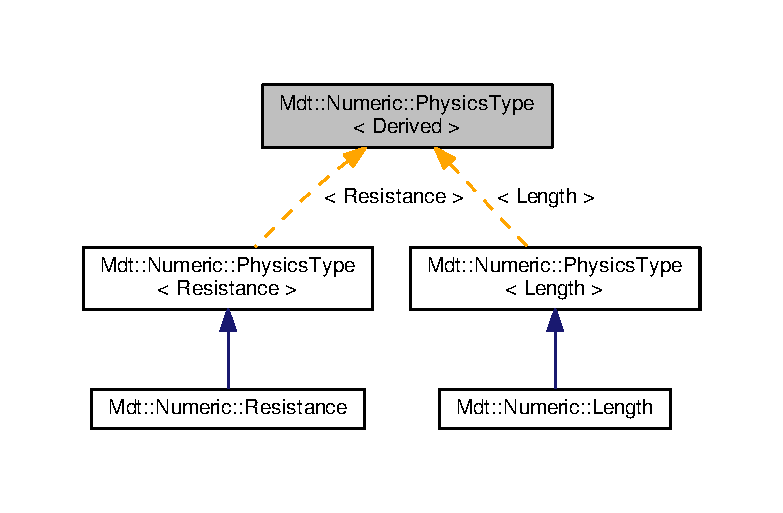
\includegraphics[width=350pt]{class_mdt_1_1_numeric_1_1_physics_type__inherit__graph}
\end{center}
\end{figure}
\subsection*{Public Member Functions}
\begin{DoxyCompactItemize}
\item 
constexpr \hyperlink{class_mdt_1_1_numeric_1_1_physics_type_a696d9d6d263562f2b07651c79901b67e}{Physics\+Type} () noexcept=default
\begin{DoxyCompactList}\small\item\em Construct a null value. \end{DoxyCompactList}\item 
constexpr \hyperlink{class_mdt_1_1_numeric_1_1_physics_type_a5a5aeff282457f7e34a4ac256640b8e9}{Physics\+Type} (\hyperlink{class_mdt_1_1_numeric_1_1_double}{Double} \hyperlink{class_mdt_1_1_numeric_1_1_physics_type_a9bc72c7175657ebbe35c0d3758fd7454}{value}) noexcept
\begin{DoxyCompactList}\small\item\em Construct a value. \end{DoxyCompactList}\item 
constexpr \hyperlink{class_mdt_1_1_numeric_1_1_double}{Double} \hyperlink{class_mdt_1_1_numeric_1_1_physics_type_a9bc72c7175657ebbe35c0d3758fd7454}{value} () const noexcept
\begin{DoxyCompactList}\small\item\em Get value. \end{DoxyCompactList}\item 
constexpr bool \hyperlink{class_mdt_1_1_numeric_1_1_physics_type_a1b845d6c259ae2e71613e7a1115cf779}{is\+Null} () const noexcept
\begin{DoxyCompactList}\small\item\em Check if value is null. \end{DoxyCompactList}\item 
constexpr Derived \hyperlink{class_mdt_1_1_numeric_1_1_physics_type_a64db52654db34e613d3cb7f673a6610f}{operator-\/} () const 
\begin{DoxyCompactList}\small\item\em Negation operator. \end{DoxyCompactList}\item 
constexpr void \hyperlink{class_mdt_1_1_numeric_1_1_physics_type_a7f2eda637785fd676a25a62972ae601c}{clear} () noexcept
\begin{DoxyCompactList}\small\item\em Clear value. \end{DoxyCompactList}\end{DoxyCompactItemize}
\subsection*{Friends}
\begin{DoxyCompactItemize}
\item 
constexpr bool \hyperlink{class_mdt_1_1_numeric_1_1_physics_type_a19bbcf82001900576c9738089b6efda8}{operator==} (const Derived \&x, const Derived \&y) noexcept
\begin{DoxyCompactList}\small\item\em Equality comparison operator. \end{DoxyCompactList}\item 
constexpr bool \hyperlink{class_mdt_1_1_numeric_1_1_physics_type_a5a810023f7517c4f4e45ce70c5da90e4}{operator!=} (const Derived \&x, const Derived \&y) noexcept
\begin{DoxyCompactList}\small\item\em Inequality comparison operator. \end{DoxyCompactList}\item 
constexpr bool \hyperlink{class_mdt_1_1_numeric_1_1_physics_type_ada4582d450e1a194357e30c1adb28fc1}{operator$<$} (const Derived \&x, const Derived \&y) noexcept
\begin{DoxyCompactList}\small\item\em Comparison operator. \end{DoxyCompactList}\item 
constexpr bool \hyperlink{class_mdt_1_1_numeric_1_1_physics_type_a0ae0bdb484fc3c65b049303fc74a7143}{operator$<$=} (const Derived \&x, const Derived \&y) noexcept
\begin{DoxyCompactList}\small\item\em Comparison operator. \end{DoxyCompactList}\item 
constexpr bool \hyperlink{class_mdt_1_1_numeric_1_1_physics_type_a4101b3710a0f4650ad71390d56730267}{operator$>$} (const Derived \&x, const Derived \&y) noexcept
\begin{DoxyCompactList}\small\item\em Comparison operator. \end{DoxyCompactList}\item 
constexpr bool \hyperlink{class_mdt_1_1_numeric_1_1_physics_type_af4568b37fec8d78d9fd949ac96a60cda}{operator$>$=} (const Derived \&x, const Derived \&y) noexcept
\begin{DoxyCompactList}\small\item\em Comparison operator. \end{DoxyCompactList}\item 
constexpr Derived \hyperlink{class_mdt_1_1_numeric_1_1_physics_type_ab6f62fa67f9f960a1be4bad528f4deaa}{operator+} (const Derived \&x, const Derived \&y) noexcept
\begin{DoxyCompactList}\small\item\em Addition operator. \end{DoxyCompactList}\item 
constexpr Derived \hyperlink{class_mdt_1_1_numeric_1_1_physics_type_a3f8c0bf444b41a8b3a2d974577d79d33}{operator-\/} (const Derived \&x, const Derived \&y) noexcept
\begin{DoxyCompactList}\small\item\em Substraction operator. \end{DoxyCompactList}\item 
constexpr Derived \hyperlink{class_mdt_1_1_numeric_1_1_physics_type_af5cf67aa0a0834c55a9507898d457b26}{operator$\ast$} (const Derived \&x, const Derived \&y) noexcept
\begin{DoxyCompactList}\small\item\em Multiplication operator. \end{DoxyCompactList}\item 
constexpr Derived \hyperlink{class_mdt_1_1_numeric_1_1_physics_type_a21498867f825277834543bf7e08ecc27}{operator/} (const Derived \&x, const Derived \&y) noexcept
\begin{DoxyCompactList}\small\item\em Division operator. \end{DoxyCompactList}\end{DoxyCompactItemize}


\subsection{Detailed Description}
\subsubsection*{template$<$typename Derived$>$\\*
class Mdt\+::\+Numeric\+::\+Physics\+Type$<$ Derived $>$}

Base class for physics type. 

\hyperlink{class_mdt_1_1_numeric_1_1_physics_type}{Physics\+Type} offers some common methods to create value types using static polymorphism (C\+R\+TP). 

Definition at line 36 of file Physics\+Type.\+h.



\subsection{Constructor \& Destructor Documentation}
\index{Mdt\+::\+Numeric\+::\+Physics\+Type@{Mdt\+::\+Numeric\+::\+Physics\+Type}!Physics\+Type@{Physics\+Type}}
\index{Physics\+Type@{Physics\+Type}!Mdt\+::\+Numeric\+::\+Physics\+Type@{Mdt\+::\+Numeric\+::\+Physics\+Type}}
\subsubsection[{\texorpdfstring{Physics\+Type() noexcept=default}{PhysicsType() noexcept=default}}]{\setlength{\rightskip}{0pt plus 5cm}template$<$typename Derived$>$ constexpr {\bf Mdt\+::\+Numeric\+::\+Physics\+Type}$<$ Derived $>$\+::{\bf Physics\+Type} (
\begin{DoxyParamCaption}
{}
\end{DoxyParamCaption}
)\hspace{0.3cm}{\ttfamily [default]}, {\ttfamily [noexcept]}}\hypertarget{class_mdt_1_1_numeric_1_1_physics_type_a696d9d6d263562f2b07651c79901b67e}{}\label{class_mdt_1_1_numeric_1_1_physics_type_a696d9d6d263562f2b07651c79901b67e}


Construct a null value. 

\index{Mdt\+::\+Numeric\+::\+Physics\+Type@{Mdt\+::\+Numeric\+::\+Physics\+Type}!Physics\+Type@{Physics\+Type}}
\index{Physics\+Type@{Physics\+Type}!Mdt\+::\+Numeric\+::\+Physics\+Type@{Mdt\+::\+Numeric\+::\+Physics\+Type}}
\subsubsection[{\texorpdfstring{Physics\+Type(\+Double value) noexcept}{PhysicsType(Double value) noexcept}}]{\setlength{\rightskip}{0pt plus 5cm}template$<$typename Derived$>$ constexpr {\bf Mdt\+::\+Numeric\+::\+Physics\+Type}$<$ Derived $>$\+::{\bf Physics\+Type} (
\begin{DoxyParamCaption}
\item[{{\bf Double}}]{value}
\end{DoxyParamCaption}
)\hspace{0.3cm}{\ttfamily [inline]}, {\ttfamily [explicit]}, {\ttfamily [noexcept]}}\hypertarget{class_mdt_1_1_numeric_1_1_physics_type_a5a5aeff282457f7e34a4ac256640b8e9}{}\label{class_mdt_1_1_numeric_1_1_physics_type_a5a5aeff282457f7e34a4ac256640b8e9}


Construct a value. 



Definition at line 46 of file Physics\+Type.\+h.



\subsection{Member Function Documentation}
\index{Mdt\+::\+Numeric\+::\+Physics\+Type@{Mdt\+::\+Numeric\+::\+Physics\+Type}!clear@{clear}}
\index{clear@{clear}!Mdt\+::\+Numeric\+::\+Physics\+Type@{Mdt\+::\+Numeric\+::\+Physics\+Type}}
\subsubsection[{\texorpdfstring{clear() noexcept}{clear() noexcept}}]{\setlength{\rightskip}{0pt plus 5cm}template$<$typename Derived$>$ constexpr void {\bf Mdt\+::\+Numeric\+::\+Physics\+Type}$<$ Derived $>$\+::clear (
\begin{DoxyParamCaption}
{}
\end{DoxyParamCaption}
)\hspace{0.3cm}{\ttfamily [inline]}, {\ttfamily [noexcept]}}\hypertarget{class_mdt_1_1_numeric_1_1_physics_type_a7f2eda637785fd676a25a62972ae601c}{}\label{class_mdt_1_1_numeric_1_1_physics_type_a7f2eda637785fd676a25a62972ae601c}


Clear value. 



Definition at line 154 of file Physics\+Type.\+h.

\index{Mdt\+::\+Numeric\+::\+Physics\+Type@{Mdt\+::\+Numeric\+::\+Physics\+Type}!is\+Null@{is\+Null}}
\index{is\+Null@{is\+Null}!Mdt\+::\+Numeric\+::\+Physics\+Type@{Mdt\+::\+Numeric\+::\+Physics\+Type}}
\subsubsection[{\texorpdfstring{is\+Null() const noexcept}{isNull() const noexcept}}]{\setlength{\rightskip}{0pt plus 5cm}template$<$typename Derived$>$ constexpr bool {\bf Mdt\+::\+Numeric\+::\+Physics\+Type}$<$ Derived $>$\+::is\+Null (
\begin{DoxyParamCaption}
{}
\end{DoxyParamCaption}
) const\hspace{0.3cm}{\ttfamily [inline]}, {\ttfamily [noexcept]}}\hypertarget{class_mdt_1_1_numeric_1_1_physics_type_a1b845d6c259ae2e71613e7a1115cf779}{}\label{class_mdt_1_1_numeric_1_1_physics_type_a1b845d6c259ae2e71613e7a1115cf779}


Check if value is null. 



Definition at line 58 of file Physics\+Type.\+h.

\index{Mdt\+::\+Numeric\+::\+Physics\+Type@{Mdt\+::\+Numeric\+::\+Physics\+Type}!operator-\/@{operator-\/}}
\index{operator-\/@{operator-\/}!Mdt\+::\+Numeric\+::\+Physics\+Type@{Mdt\+::\+Numeric\+::\+Physics\+Type}}
\subsubsection[{\texorpdfstring{operator-\/() const }{operator-() const }}]{\setlength{\rightskip}{0pt plus 5cm}template$<$typename Derived$>$ constexpr Derived {\bf Mdt\+::\+Numeric\+::\+Physics\+Type}$<$ Derived $>$\+::operator-\/ (
\begin{DoxyParamCaption}
{}
\end{DoxyParamCaption}
) const\hspace{0.3cm}{\ttfamily [inline]}}\hypertarget{class_mdt_1_1_numeric_1_1_physics_type_a64db52654db34e613d3cb7f673a6610f}{}\label{class_mdt_1_1_numeric_1_1_physics_type_a64db52654db34e613d3cb7f673a6610f}


Negation operator. 



Definition at line 131 of file Physics\+Type.\+h.

\index{Mdt\+::\+Numeric\+::\+Physics\+Type@{Mdt\+::\+Numeric\+::\+Physics\+Type}!value@{value}}
\index{value@{value}!Mdt\+::\+Numeric\+::\+Physics\+Type@{Mdt\+::\+Numeric\+::\+Physics\+Type}}
\subsubsection[{\texorpdfstring{value() const noexcept}{value() const noexcept}}]{\setlength{\rightskip}{0pt plus 5cm}template$<$typename Derived$>$ constexpr {\bf Double} {\bf Mdt\+::\+Numeric\+::\+Physics\+Type}$<$ Derived $>$\+::value (
\begin{DoxyParamCaption}
{}
\end{DoxyParamCaption}
) const\hspace{0.3cm}{\ttfamily [inline]}, {\ttfamily [noexcept]}}\hypertarget{class_mdt_1_1_numeric_1_1_physics_type_a9bc72c7175657ebbe35c0d3758fd7454}{}\label{class_mdt_1_1_numeric_1_1_physics_type_a9bc72c7175657ebbe35c0d3758fd7454}


Get value. 



Definition at line 51 of file Physics\+Type.\+h.



\subsection{Friends And Related Function Documentation}
\index{Mdt\+::\+Numeric\+::\+Physics\+Type@{Mdt\+::\+Numeric\+::\+Physics\+Type}!operator"!=@{operator"!=}}
\index{operator"!=@{operator"!=}!Mdt\+::\+Numeric\+::\+Physics\+Type@{Mdt\+::\+Numeric\+::\+Physics\+Type}}
\subsubsection[{\texorpdfstring{operator"!=}{operator!=}}]{\setlength{\rightskip}{0pt plus 5cm}template$<$typename Derived$>$ constexpr bool operator!= (
\begin{DoxyParamCaption}
\item[{const Derived \&}]{x, }
\item[{const Derived \&}]{y}
\end{DoxyParamCaption}
)\hspace{0.3cm}{\ttfamily [friend]}}\hypertarget{class_mdt_1_1_numeric_1_1_physics_type_a5a810023f7517c4f4e45ce70c5da90e4}{}\label{class_mdt_1_1_numeric_1_1_physics_type_a5a810023f7517c4f4e45ce70c5da90e4}


Inequality comparison operator. 

\begin{DoxySeeAlso}{See also}
\hyperlink{class_mdt_1_1_numeric_1_1_physics_type_a19bbcf82001900576c9738089b6efda8}{operator==()} 
\end{DoxySeeAlso}


Definition at line 76 of file Physics\+Type.\+h.

\index{Mdt\+::\+Numeric\+::\+Physics\+Type@{Mdt\+::\+Numeric\+::\+Physics\+Type}!operator$\ast$@{operator$\ast$}}
\index{operator$\ast$@{operator$\ast$}!Mdt\+::\+Numeric\+::\+Physics\+Type@{Mdt\+::\+Numeric\+::\+Physics\+Type}}
\subsubsection[{\texorpdfstring{operator$\ast$}{operator*}}]{\setlength{\rightskip}{0pt plus 5cm}template$<$typename Derived$>$ constexpr Derived operator$\ast$ (
\begin{DoxyParamCaption}
\item[{const Derived \&}]{x, }
\item[{const Derived \&}]{y}
\end{DoxyParamCaption}
)\hspace{0.3cm}{\ttfamily [friend]}}\hypertarget{class_mdt_1_1_numeric_1_1_physics_type_af5cf67aa0a0834c55a9507898d457b26}{}\label{class_mdt_1_1_numeric_1_1_physics_type_af5cf67aa0a0834c55a9507898d457b26}


Multiplication operator. 



Definition at line 139 of file Physics\+Type.\+h.

\index{Mdt\+::\+Numeric\+::\+Physics\+Type@{Mdt\+::\+Numeric\+::\+Physics\+Type}!operator+@{operator+}}
\index{operator+@{operator+}!Mdt\+::\+Numeric\+::\+Physics\+Type@{Mdt\+::\+Numeric\+::\+Physics\+Type}}
\subsubsection[{\texorpdfstring{operator+}{operator+}}]{\setlength{\rightskip}{0pt plus 5cm}template$<$typename Derived$>$ constexpr Derived operator+ (
\begin{DoxyParamCaption}
\item[{const Derived \&}]{x, }
\item[{const Derived \&}]{y}
\end{DoxyParamCaption}
)\hspace{0.3cm}{\ttfamily [friend]}}\hypertarget{class_mdt_1_1_numeric_1_1_physics_type_ab6f62fa67f9f960a1be4bad528f4deaa}{}\label{class_mdt_1_1_numeric_1_1_physics_type_ab6f62fa67f9f960a1be4bad528f4deaa}


Addition operator. 



Definition at line 116 of file Physics\+Type.\+h.

\index{Mdt\+::\+Numeric\+::\+Physics\+Type@{Mdt\+::\+Numeric\+::\+Physics\+Type}!operator-\/@{operator-\/}}
\index{operator-\/@{operator-\/}!Mdt\+::\+Numeric\+::\+Physics\+Type@{Mdt\+::\+Numeric\+::\+Physics\+Type}}
\subsubsection[{\texorpdfstring{operator-\/}{operator-}}]{\setlength{\rightskip}{0pt plus 5cm}template$<$typename Derived$>$ constexpr Derived operator-\/ (
\begin{DoxyParamCaption}
\item[{const Derived \&}]{x, }
\item[{const Derived \&}]{y}
\end{DoxyParamCaption}
)\hspace{0.3cm}{\ttfamily [friend]}}\hypertarget{class_mdt_1_1_numeric_1_1_physics_type_a3f8c0bf444b41a8b3a2d974577d79d33}{}\label{class_mdt_1_1_numeric_1_1_physics_type_a3f8c0bf444b41a8b3a2d974577d79d33}


Substraction operator. 



Definition at line 124 of file Physics\+Type.\+h.

\index{Mdt\+::\+Numeric\+::\+Physics\+Type@{Mdt\+::\+Numeric\+::\+Physics\+Type}!operator/@{operator/}}
\index{operator/@{operator/}!Mdt\+::\+Numeric\+::\+Physics\+Type@{Mdt\+::\+Numeric\+::\+Physics\+Type}}
\subsubsection[{\texorpdfstring{operator/}{operator/}}]{\setlength{\rightskip}{0pt plus 5cm}template$<$typename Derived$>$ constexpr Derived operator/ (
\begin{DoxyParamCaption}
\item[{const Derived \&}]{x, }
\item[{const Derived \&}]{y}
\end{DoxyParamCaption}
)\hspace{0.3cm}{\ttfamily [friend]}}\hypertarget{class_mdt_1_1_numeric_1_1_physics_type_a21498867f825277834543bf7e08ecc27}{}\label{class_mdt_1_1_numeric_1_1_physics_type_a21498867f825277834543bf7e08ecc27}


Division operator. 



Definition at line 147 of file Physics\+Type.\+h.

\index{Mdt\+::\+Numeric\+::\+Physics\+Type@{Mdt\+::\+Numeric\+::\+Physics\+Type}!operator$<$@{operator$<$}}
\index{operator$<$@{operator$<$}!Mdt\+::\+Numeric\+::\+Physics\+Type@{Mdt\+::\+Numeric\+::\+Physics\+Type}}
\subsubsection[{\texorpdfstring{operator$<$}{operator<}}]{\setlength{\rightskip}{0pt plus 5cm}template$<$typename Derived$>$ constexpr bool operator$<$ (
\begin{DoxyParamCaption}
\item[{const Derived \&}]{x, }
\item[{const Derived \&}]{y}
\end{DoxyParamCaption}
)\hspace{0.3cm}{\ttfamily [friend]}}\hypertarget{class_mdt_1_1_numeric_1_1_physics_type_ada4582d450e1a194357e30c1adb28fc1}{}\label{class_mdt_1_1_numeric_1_1_physics_type_ada4582d450e1a194357e30c1adb28fc1}


Comparison operator. 



Definition at line 84 of file Physics\+Type.\+h.

\index{Mdt\+::\+Numeric\+::\+Physics\+Type@{Mdt\+::\+Numeric\+::\+Physics\+Type}!operator$<$=@{operator$<$=}}
\index{operator$<$=@{operator$<$=}!Mdt\+::\+Numeric\+::\+Physics\+Type@{Mdt\+::\+Numeric\+::\+Physics\+Type}}
\subsubsection[{\texorpdfstring{operator$<$=}{operator<=}}]{\setlength{\rightskip}{0pt plus 5cm}template$<$typename Derived$>$ constexpr bool operator$<$= (
\begin{DoxyParamCaption}
\item[{const Derived \&}]{x, }
\item[{const Derived \&}]{y}
\end{DoxyParamCaption}
)\hspace{0.3cm}{\ttfamily [friend]}}\hypertarget{class_mdt_1_1_numeric_1_1_physics_type_a0ae0bdb484fc3c65b049303fc74a7143}{}\label{class_mdt_1_1_numeric_1_1_physics_type_a0ae0bdb484fc3c65b049303fc74a7143}


Comparison operator. 



Definition at line 92 of file Physics\+Type.\+h.

\index{Mdt\+::\+Numeric\+::\+Physics\+Type@{Mdt\+::\+Numeric\+::\+Physics\+Type}!operator==@{operator==}}
\index{operator==@{operator==}!Mdt\+::\+Numeric\+::\+Physics\+Type@{Mdt\+::\+Numeric\+::\+Physics\+Type}}
\subsubsection[{\texorpdfstring{operator==}{operator==}}]{\setlength{\rightskip}{0pt plus 5cm}template$<$typename Derived$>$ constexpr bool operator== (
\begin{DoxyParamCaption}
\item[{const Derived \&}]{x, }
\item[{const Derived \&}]{y}
\end{DoxyParamCaption}
)\hspace{0.3cm}{\ttfamily [friend]}}\hypertarget{class_mdt_1_1_numeric_1_1_physics_type_a19bbcf82001900576c9738089b6efda8}{}\label{class_mdt_1_1_numeric_1_1_physics_type_a19bbcf82001900576c9738089b6efda8}


Equality comparison operator. 



Definition at line 66 of file Physics\+Type.\+h.

\index{Mdt\+::\+Numeric\+::\+Physics\+Type@{Mdt\+::\+Numeric\+::\+Physics\+Type}!operator$>$@{operator$>$}}
\index{operator$>$@{operator$>$}!Mdt\+::\+Numeric\+::\+Physics\+Type@{Mdt\+::\+Numeric\+::\+Physics\+Type}}
\subsubsection[{\texorpdfstring{operator$>$}{operator>}}]{\setlength{\rightskip}{0pt plus 5cm}template$<$typename Derived$>$ constexpr bool operator$>$ (
\begin{DoxyParamCaption}
\item[{const Derived \&}]{x, }
\item[{const Derived \&}]{y}
\end{DoxyParamCaption}
)\hspace{0.3cm}{\ttfamily [friend]}}\hypertarget{class_mdt_1_1_numeric_1_1_physics_type_a4101b3710a0f4650ad71390d56730267}{}\label{class_mdt_1_1_numeric_1_1_physics_type_a4101b3710a0f4650ad71390d56730267}


Comparison operator. 



Definition at line 100 of file Physics\+Type.\+h.

\index{Mdt\+::\+Numeric\+::\+Physics\+Type@{Mdt\+::\+Numeric\+::\+Physics\+Type}!operator$>$=@{operator$>$=}}
\index{operator$>$=@{operator$>$=}!Mdt\+::\+Numeric\+::\+Physics\+Type@{Mdt\+::\+Numeric\+::\+Physics\+Type}}
\subsubsection[{\texorpdfstring{operator$>$=}{operator>=}}]{\setlength{\rightskip}{0pt plus 5cm}template$<$typename Derived$>$ constexpr bool operator$>$= (
\begin{DoxyParamCaption}
\item[{const Derived \&}]{x, }
\item[{const Derived \&}]{y}
\end{DoxyParamCaption}
)\hspace{0.3cm}{\ttfamily [friend]}}\hypertarget{class_mdt_1_1_numeric_1_1_physics_type_af4568b37fec8d78d9fd949ac96a60cda}{}\label{class_mdt_1_1_numeric_1_1_physics_type_af4568b37fec8d78d9fd949ac96a60cda}


Comparison operator. 



Definition at line 108 of file Physics\+Type.\+h.



The documentation for this class was generated from the following file\+:\begin{DoxyCompactItemize}
\item 
libs/\+Numeric/src/\+Mdt/\+Numeric/Physics\+Type.\+h\end{DoxyCompactItemize}

\hypertarget{class_mdt_1_1_deploy_utils_1_1_platform}{}\section{Mdt\+:\+:Deploy\+Utils\+:\+:Platform Class Reference}
\label{class_mdt_1_1_deploy_utils_1_1_platform}\index{Mdt\+::\+Deploy\+Utils\+::\+Platform@{Mdt\+::\+Deploy\+Utils\+::\+Platform}}


Definition of a platform.  




{\ttfamily \#include $<$Platform.\+h$>$}

\subsection*{Public Member Functions}
\begin{DoxyCompactItemize}
\item 
\hyperlink{class_mdt_1_1_deploy_utils_1_1_platform_a1d0bfc4226c34681de02fb71bdf21ab1}{Platform} (Operating\+System os=\hyperlink{class_mdt_1_1_deploy_utils_1_1_platform_aa9c466ca43cea94e751b73f8270fe4bb}{native\+Operating\+System}(), Compiler \hyperlink{class_mdt_1_1_deploy_utils_1_1_platform_a453beb4e9409bc5c1473ffae3f211dc0}{compiler}=\hyperlink{class_mdt_1_1_deploy_utils_1_1_platform_aeca6535d32ac63294f3f8dfcb9b996a7}{native\+Compiler}(), Processor \hyperlink{class_mdt_1_1_deploy_utils_1_1_platform_a5f94968dbefcbe843b503fae9afb9ce6}{processor}=\hyperlink{class_mdt_1_1_deploy_utils_1_1_platform_afcf216e9f71ad3df91588dd1e96e05ee}{native\+Processor}())
\begin{DoxyCompactList}\small\item\em Construct a platform. \end{DoxyCompactList}\item 
Operating\+System \hyperlink{class_mdt_1_1_deploy_utils_1_1_platform_a564312f1a3df51c9028ba35e05fb4c45}{operating\+System} () const 
\begin{DoxyCompactList}\small\item\em Get operating system. \end{DoxyCompactList}\item 
Compiler \hyperlink{class_mdt_1_1_deploy_utils_1_1_platform_a453beb4e9409bc5c1473ffae3f211dc0}{compiler} () const 
\begin{DoxyCompactList}\small\item\em Get compiler. \end{DoxyCompactList}\item 
Processor \hyperlink{class_mdt_1_1_deploy_utils_1_1_platform_a5f94968dbefcbe843b503fae9afb9ce6}{processor} () const 
\begin{DoxyCompactList}\small\item\em Get processor. \end{DoxyCompactList}\end{DoxyCompactItemize}
\subsection*{Static Public Member Functions}
\begin{DoxyCompactItemize}
\item 
static Operating\+System \hyperlink{class_mdt_1_1_deploy_utils_1_1_platform_aa9c466ca43cea94e751b73f8270fe4bb}{native\+Operating\+System} ()
\begin{DoxyCompactList}\small\item\em Get native operating system. \end{DoxyCompactList}\item 
static Compiler \hyperlink{class_mdt_1_1_deploy_utils_1_1_platform_aeca6535d32ac63294f3f8dfcb9b996a7}{native\+Compiler} ()
\begin{DoxyCompactList}\small\item\em Get native compiler. \end{DoxyCompactList}\item 
static Processor \hyperlink{class_mdt_1_1_deploy_utils_1_1_platform_afcf216e9f71ad3df91588dd1e96e05ee}{native\+Processor} ()
\begin{DoxyCompactList}\small\item\em Get native processor. \end{DoxyCompactList}\end{DoxyCompactItemize}


\subsection{Detailed Description}
Definition of a platform. 

\begin{DoxyRefDesc}{Todo}
\item[\hyperlink{todo__todo000005}{Todo}]Currently, we have a very poor support. \end{DoxyRefDesc}


Definition at line 34 of file Platform.\+h.



\subsection{Constructor \& Destructor Documentation}
\index{Mdt\+::\+Deploy\+Utils\+::\+Platform@{Mdt\+::\+Deploy\+Utils\+::\+Platform}!Platform@{Platform}}
\index{Platform@{Platform}!Mdt\+::\+Deploy\+Utils\+::\+Platform@{Mdt\+::\+Deploy\+Utils\+::\+Platform}}
\subsubsection[{\texorpdfstring{Platform(\+Operating\+System os=native\+Operating\+System(), Compiler compiler=native\+Compiler(), Processor processor=native\+Processor())}{Platform(OperatingSystem os=nativeOperatingSystem(), Compiler compiler=nativeCompiler(), Processor processor=nativeProcessor())}}]{\setlength{\rightskip}{0pt plus 5cm}Mdt\+::\+Deploy\+Utils\+::\+Platform\+::\+Platform (
\begin{DoxyParamCaption}
\item[{Operating\+System}]{os = {\ttfamily {\bf native\+Operating\+System}()}, }
\item[{Compiler}]{compiler = {\ttfamily {\bf native\+Compiler}()}, }
\item[{Processor}]{processor = {\ttfamily {\bf native\+Processor}()}}
\end{DoxyParamCaption}
)}\hypertarget{class_mdt_1_1_deploy_utils_1_1_platform_a1d0bfc4226c34681de02fb71bdf21ab1}{}\label{class_mdt_1_1_deploy_utils_1_1_platform_a1d0bfc4226c34681de02fb71bdf21ab1}


Construct a platform. 



Definition at line 26 of file Platform.\+cpp.



\subsection{Member Function Documentation}
\index{Mdt\+::\+Deploy\+Utils\+::\+Platform@{Mdt\+::\+Deploy\+Utils\+::\+Platform}!compiler@{compiler}}
\index{compiler@{compiler}!Mdt\+::\+Deploy\+Utils\+::\+Platform@{Mdt\+::\+Deploy\+Utils\+::\+Platform}}
\subsubsection[{\texorpdfstring{compiler() const }{compiler() const }}]{\setlength{\rightskip}{0pt plus 5cm}Compiler Mdt\+::\+Deploy\+Utils\+::\+Platform\+::compiler (
\begin{DoxyParamCaption}
{}
\end{DoxyParamCaption}
) const\hspace{0.3cm}{\ttfamily [inline]}}\hypertarget{class_mdt_1_1_deploy_utils_1_1_platform_a453beb4e9409bc5c1473ffae3f211dc0}{}\label{class_mdt_1_1_deploy_utils_1_1_platform_a453beb4e9409bc5c1473ffae3f211dc0}


Get compiler. 



Definition at line 55 of file Platform.\+h.

\index{Mdt\+::\+Deploy\+Utils\+::\+Platform@{Mdt\+::\+Deploy\+Utils\+::\+Platform}!native\+Compiler@{native\+Compiler}}
\index{native\+Compiler@{native\+Compiler}!Mdt\+::\+Deploy\+Utils\+::\+Platform@{Mdt\+::\+Deploy\+Utils\+::\+Platform}}
\subsubsection[{\texorpdfstring{native\+Compiler()}{nativeCompiler()}}]{\setlength{\rightskip}{0pt plus 5cm}Compiler Mdt\+::\+Deploy\+Utils\+::\+Platform\+::native\+Compiler (
\begin{DoxyParamCaption}
{}
\end{DoxyParamCaption}
)\hspace{0.3cm}{\ttfamily [static]}}\hypertarget{class_mdt_1_1_deploy_utils_1_1_platform_aeca6535d32ac63294f3f8dfcb9b996a7}{}\label{class_mdt_1_1_deploy_utils_1_1_platform_aeca6535d32ac63294f3f8dfcb9b996a7}


Get native compiler. 



Definition at line 44 of file Platform.\+cpp.

\index{Mdt\+::\+Deploy\+Utils\+::\+Platform@{Mdt\+::\+Deploy\+Utils\+::\+Platform}!native\+Operating\+System@{native\+Operating\+System}}
\index{native\+Operating\+System@{native\+Operating\+System}!Mdt\+::\+Deploy\+Utils\+::\+Platform@{Mdt\+::\+Deploy\+Utils\+::\+Platform}}
\subsubsection[{\texorpdfstring{native\+Operating\+System()}{nativeOperatingSystem()}}]{\setlength{\rightskip}{0pt plus 5cm}Operating\+System Mdt\+::\+Deploy\+Utils\+::\+Platform\+::native\+Operating\+System (
\begin{DoxyParamCaption}
{}
\end{DoxyParamCaption}
)\hspace{0.3cm}{\ttfamily [static]}}\hypertarget{class_mdt_1_1_deploy_utils_1_1_platform_aa9c466ca43cea94e751b73f8270fe4bb}{}\label{class_mdt_1_1_deploy_utils_1_1_platform_aa9c466ca43cea94e751b73f8270fe4bb}


Get native operating system. 



Definition at line 33 of file Platform.\+cpp.

\index{Mdt\+::\+Deploy\+Utils\+::\+Platform@{Mdt\+::\+Deploy\+Utils\+::\+Platform}!native\+Processor@{native\+Processor}}
\index{native\+Processor@{native\+Processor}!Mdt\+::\+Deploy\+Utils\+::\+Platform@{Mdt\+::\+Deploy\+Utils\+::\+Platform}}
\subsubsection[{\texorpdfstring{native\+Processor()}{nativeProcessor()}}]{\setlength{\rightskip}{0pt plus 5cm}Processor Mdt\+::\+Deploy\+Utils\+::\+Platform\+::native\+Processor (
\begin{DoxyParamCaption}
{}
\end{DoxyParamCaption}
)\hspace{0.3cm}{\ttfamily [static]}}\hypertarget{class_mdt_1_1_deploy_utils_1_1_platform_afcf216e9f71ad3df91588dd1e96e05ee}{}\label{class_mdt_1_1_deploy_utils_1_1_platform_afcf216e9f71ad3df91588dd1e96e05ee}


Get native processor. 



Definition at line 53 of file Platform.\+cpp.

\index{Mdt\+::\+Deploy\+Utils\+::\+Platform@{Mdt\+::\+Deploy\+Utils\+::\+Platform}!operating\+System@{operating\+System}}
\index{operating\+System@{operating\+System}!Mdt\+::\+Deploy\+Utils\+::\+Platform@{Mdt\+::\+Deploy\+Utils\+::\+Platform}}
\subsubsection[{\texorpdfstring{operating\+System() const }{operatingSystem() const }}]{\setlength{\rightskip}{0pt plus 5cm}Operating\+System Mdt\+::\+Deploy\+Utils\+::\+Platform\+::operating\+System (
\begin{DoxyParamCaption}
{}
\end{DoxyParamCaption}
) const\hspace{0.3cm}{\ttfamily [inline]}}\hypertarget{class_mdt_1_1_deploy_utils_1_1_platform_a564312f1a3df51c9028ba35e05fb4c45}{}\label{class_mdt_1_1_deploy_utils_1_1_platform_a564312f1a3df51c9028ba35e05fb4c45}


Get operating system. 



Definition at line 44 of file Platform.\+h.

\index{Mdt\+::\+Deploy\+Utils\+::\+Platform@{Mdt\+::\+Deploy\+Utils\+::\+Platform}!processor@{processor}}
\index{processor@{processor}!Mdt\+::\+Deploy\+Utils\+::\+Platform@{Mdt\+::\+Deploy\+Utils\+::\+Platform}}
\subsubsection[{\texorpdfstring{processor() const }{processor() const }}]{\setlength{\rightskip}{0pt plus 5cm}Processor Mdt\+::\+Deploy\+Utils\+::\+Platform\+::processor (
\begin{DoxyParamCaption}
{}
\end{DoxyParamCaption}
) const\hspace{0.3cm}{\ttfamily [inline]}}\hypertarget{class_mdt_1_1_deploy_utils_1_1_platform_a5f94968dbefcbe843b503fae9afb9ce6}{}\label{class_mdt_1_1_deploy_utils_1_1_platform_a5f94968dbefcbe843b503fae9afb9ce6}


Get processor. 



Definition at line 66 of file Platform.\+h.



The documentation for this class was generated from the following files\+:\begin{DoxyCompactItemize}
\item 
libs/\+Deploy\+Utils\+\_\+\+Core/src/\+Mdt/\+Deploy\+Utils/Platform.\+h\item 
libs/\+Deploy\+Utils\+\_\+\+Core/src/\+Mdt/\+Deploy\+Utils/Platform.\+cpp\end{DoxyCompactItemize}

\hypertarget{class_mdt_1_1_deploy_utils_1_1_qt_library}{}\section{Mdt\+:\+:Deploy\+Utils\+:\+:Qt\+Library Class Reference}
\label{class_mdt_1_1_deploy_utils_1_1_qt_library}\index{Mdt\+::\+Deploy\+Utils\+::\+Qt\+Library@{Mdt\+::\+Deploy\+Utils\+::\+Qt\+Library}}


\hyperlink{class_mdt_1_1_deploy_utils_1_1_qt_library}{Qt\+Library} offers some utilities specific to Qt libraries.  




{\ttfamily \#include $<$Qt\+Library.\+h$>$}



Inheritance diagram for Mdt\+:\+:Deploy\+Utils\+:\+:Qt\+Library\+:
\nopagebreak
\begin{figure}[H]
\begin{center}
\leavevmode
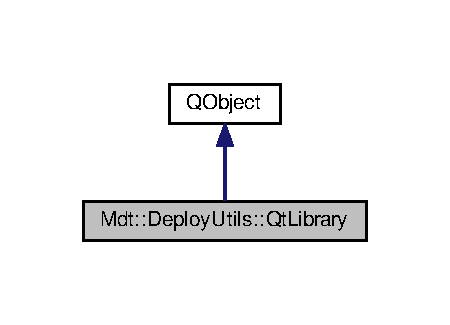
\includegraphics[width=216pt]{class_mdt_1_1_deploy_utils_1_1_qt_library__inherit__graph}
\end{center}
\end{figure}


Collaboration diagram for Mdt\+:\+:Deploy\+Utils\+:\+:Qt\+Library\+:
\nopagebreak
\begin{figure}[H]
\begin{center}
\leavevmode
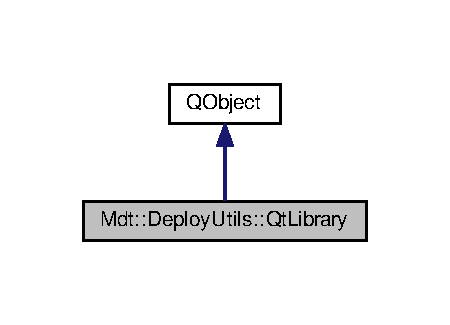
\includegraphics[width=216pt]{class_mdt_1_1_deploy_utils_1_1_qt_library__coll__graph}
\end{center}
\end{figure}
\subsection*{Public Member Functions}
\begin{DoxyCompactItemize}
\item 
\hyperlink{class_mdt_1_1_deploy_utils_1_1_library_info_list}{Library\+Info\+List} \hyperlink{class_mdt_1_1_deploy_utils_1_1_qt_library_a4b3c9f30edc9bea8904205eb450e9060}{find\+Library\+Plugins} (const \hyperlink{class_mdt_1_1_deploy_utils_1_1_library_info}{Library\+Info} \&qt\+Library, const \hyperlink{class_mdt_1_1_deploy_utils_1_1_path_list}{Path\+List} \&search\+First\+Path\+Prefix\+List)
\begin{DoxyCompactList}\small\item\em Find plugins for a Qt library. \end{DoxyCompactList}\item 
\hyperlink{class_mdt_1_1_deploy_utils_1_1_library_info_list}{Library\+Info\+List} \hyperlink{class_mdt_1_1_deploy_utils_1_1_qt_library_a268a9e397c091779eb5f961f40c7d3e6}{find\+Libraries\+Plugins} (const \hyperlink{class_mdt_1_1_deploy_utils_1_1_library_info_list}{Library\+Info\+List} \&qt\+Libraries, const \hyperlink{class_mdt_1_1_deploy_utils_1_1_path_list}{Path\+List} \&search\+First\+Path\+Prefix\+List)
\begin{DoxyCompactList}\small\item\em Find plugins for a list of Qt libraries. \end{DoxyCompactList}\end{DoxyCompactItemize}
\subsection*{Static Public Member Functions}
\begin{DoxyCompactItemize}
\item 
static \hyperlink{class_mdt_1_1_deploy_utils_1_1_library_info_list}{Library\+Info\+List} \hyperlink{class_mdt_1_1_deploy_utils_1_1_qt_library_a0c576f08e6aa61164cd9d5c8faad475c}{get\+Qt\+Libraries} (const \hyperlink{class_mdt_1_1_deploy_utils_1_1_library_info_list}{Library\+Info\+List} \&libraries)
\begin{DoxyCompactList}\small\item\em Get Qt libraries out of {\itshape libraries}. \end{DoxyCompactList}\item 
static Qt\+Module \hyperlink{class_mdt_1_1_deploy_utils_1_1_qt_library_aa54f542e548bcab6da5e8a9696169a94}{module} (const \hyperlink{class_mdt_1_1_deploy_utils_1_1_library_info}{Library\+Info} \&qt\+Library)
\begin{DoxyCompactList}\small\item\em Get the module to which {\itshape qt\+Library} is part of. \end{DoxyCompactList}\item 
static \hyperlink{class_mdt_1_1_deploy_utils_1_1_qt_module_list}{Qt\+Module\+List} \hyperlink{class_mdt_1_1_deploy_utils_1_1_qt_library_ac7fd0c6a555df4f4ca7361e36f1a4ae4}{get\+Modules} (const \hyperlink{class_mdt_1_1_deploy_utils_1_1_library_info_list}{Library\+Info\+List} \&qt\+Libraries)
\begin{DoxyCompactList}\small\item\em Get a list that contains modules for {\itshape qt\+Libraries}. \end{DoxyCompactList}\item 
static Q\+String\+List \hyperlink{class_mdt_1_1_deploy_utils_1_1_qt_library_a50c96c2d0b892da7c41d50ca627191bd}{get\+Plugins\+Directories} (Qt\+Module \hyperlink{class_mdt_1_1_deploy_utils_1_1_qt_library_aa54f542e548bcab6da5e8a9696169a94}{module})
\begin{DoxyCompactList}\small\item\em Get plugins directories for {\itshape module}. \end{DoxyCompactList}\item 
static Q\+String\+List \hyperlink{class_mdt_1_1_deploy_utils_1_1_qt_library_ab555321caadc47fcb9458ba466287702}{get\+Plugins\+Directories} (const \hyperlink{class_mdt_1_1_deploy_utils_1_1_qt_module_list}{Qt\+Module\+List} \&modules)
\begin{DoxyCompactList}\small\item\em Get plugins directories for {\itshape modules}. \end{DoxyCompactList}\end{DoxyCompactItemize}


\subsection{Detailed Description}
\hyperlink{class_mdt_1_1_deploy_utils_1_1_qt_library}{Qt\+Library} offers some utilities specific to Qt libraries. 

Definition at line 39 of file Qt\+Library.\+h.



\subsection{Member Function Documentation}
\index{Mdt\+::\+Deploy\+Utils\+::\+Qt\+Library@{Mdt\+::\+Deploy\+Utils\+::\+Qt\+Library}!find\+Libraries\+Plugins@{find\+Libraries\+Plugins}}
\index{find\+Libraries\+Plugins@{find\+Libraries\+Plugins}!Mdt\+::\+Deploy\+Utils\+::\+Qt\+Library@{Mdt\+::\+Deploy\+Utils\+::\+Qt\+Library}}
\subsubsection[{\texorpdfstring{find\+Libraries\+Plugins(const Library\+Info\+List \&qt\+Libraries, const Path\+List \&search\+First\+Path\+Prefix\+List)}{findLibrariesPlugins(const LibraryInfoList &qtLibraries, const PathList &searchFirstPathPrefixList)}}]{\setlength{\rightskip}{0pt plus 5cm}{\bf Library\+Info\+List} Mdt\+::\+Deploy\+Utils\+::\+Qt\+Library\+::find\+Libraries\+Plugins (
\begin{DoxyParamCaption}
\item[{const {\bf Library\+Info\+List} \&}]{qt\+Libraries, }
\item[{const {\bf Path\+List} \&}]{search\+First\+Path\+Prefix\+List}
\end{DoxyParamCaption}
)}\hypertarget{class_mdt_1_1_deploy_utils_1_1_qt_library_a268a9e397c091779eb5f961f40c7d3e6}{}\label{class_mdt_1_1_deploy_utils_1_1_qt_library_a268a9e397c091779eb5f961f40c7d3e6}


Find plugins for a list of Qt libraries. 

\begin{DoxySeeAlso}{See also}
\hyperlink{class_mdt_1_1_deploy_utils_1_1_qt_library_a4b3c9f30edc9bea8904205eb450e9060}{find\+Library\+Plugins()} 
\end{DoxySeeAlso}


Definition at line 63 of file Qt\+Library.\+cpp.

\index{Mdt\+::\+Deploy\+Utils\+::\+Qt\+Library@{Mdt\+::\+Deploy\+Utils\+::\+Qt\+Library}!find\+Library\+Plugins@{find\+Library\+Plugins}}
\index{find\+Library\+Plugins@{find\+Library\+Plugins}!Mdt\+::\+Deploy\+Utils\+::\+Qt\+Library@{Mdt\+::\+Deploy\+Utils\+::\+Qt\+Library}}
\subsubsection[{\texorpdfstring{find\+Library\+Plugins(const Library\+Info \&qt\+Library, const Path\+List \&search\+First\+Path\+Prefix\+List)}{findLibraryPlugins(const LibraryInfo &qtLibrary, const PathList &searchFirstPathPrefixList)}}]{\setlength{\rightskip}{0pt plus 5cm}{\bf Library\+Info\+List} Mdt\+::\+Deploy\+Utils\+::\+Qt\+Library\+::find\+Library\+Plugins (
\begin{DoxyParamCaption}
\item[{const {\bf Library\+Info} \&}]{qt\+Library, }
\item[{const {\bf Path\+List} \&}]{search\+First\+Path\+Prefix\+List}
\end{DoxyParamCaption}
)}\hypertarget{class_mdt_1_1_deploy_utils_1_1_qt_library_a4b3c9f30edc9bea8904205eb450e9060}{}\label{class_mdt_1_1_deploy_utils_1_1_qt_library_a4b3c9f30edc9bea8904205eb450e9060}


Find plugins for a Qt library. 

Will first deduce Qt plugins directories attached to {\itshape qt\+Library} using \hyperlink{class_mdt_1_1_deploy_utils_1_1_qt_library_a50c96c2d0b892da7c41d50ca627191bd}{get\+Plugins\+Directories(\+Qt\+Module)}, then find the existing ones.

{\itshape search\+First\+Path\+Prefix\+List} is a list of paths to the root of a Qt installation. Plugins are serached first in each item of {\itshape search\+First\+Path\+Prefix\+List}, then in system library prefix paths. For each path in all mentionned path prefixes, plugins are searched in qt5/plugins, then plugins subdirectories. 

Definition at line 36 of file Qt\+Library.\+cpp.

\index{Mdt\+::\+Deploy\+Utils\+::\+Qt\+Library@{Mdt\+::\+Deploy\+Utils\+::\+Qt\+Library}!get\+Modules@{get\+Modules}}
\index{get\+Modules@{get\+Modules}!Mdt\+::\+Deploy\+Utils\+::\+Qt\+Library@{Mdt\+::\+Deploy\+Utils\+::\+Qt\+Library}}
\subsubsection[{\texorpdfstring{get\+Modules(const Library\+Info\+List \&qt\+Libraries)}{getModules(const LibraryInfoList &qtLibraries)}}]{\setlength{\rightskip}{0pt plus 5cm}{\bf Qt\+Module\+List} Mdt\+::\+Deploy\+Utils\+::\+Qt\+Library\+::get\+Modules (
\begin{DoxyParamCaption}
\item[{const {\bf Library\+Info\+List} \&}]{qt\+Libraries}
\end{DoxyParamCaption}
)\hspace{0.3cm}{\ttfamily [static]}}\hypertarget{class_mdt_1_1_deploy_utils_1_1_qt_library_ac7fd0c6a555df4f4ca7361e36f1a4ae4}{}\label{class_mdt_1_1_deploy_utils_1_1_qt_library_ac7fd0c6a555df4f4ca7361e36f1a4ae4}


Get a list that contains modules for {\itshape qt\+Libraries}. 



Definition at line 122 of file Qt\+Library.\+cpp.

\index{Mdt\+::\+Deploy\+Utils\+::\+Qt\+Library@{Mdt\+::\+Deploy\+Utils\+::\+Qt\+Library}!get\+Plugins\+Directories@{get\+Plugins\+Directories}}
\index{get\+Plugins\+Directories@{get\+Plugins\+Directories}!Mdt\+::\+Deploy\+Utils\+::\+Qt\+Library@{Mdt\+::\+Deploy\+Utils\+::\+Qt\+Library}}
\subsubsection[{\texorpdfstring{get\+Plugins\+Directories(\+Qt\+Module module)}{getPluginsDirectories(QtModule module)}}]{\setlength{\rightskip}{0pt plus 5cm}Q\+String\+List Mdt\+::\+Deploy\+Utils\+::\+Qt\+Library\+::get\+Plugins\+Directories (
\begin{DoxyParamCaption}
\item[{Qt\+Module}]{module}
\end{DoxyParamCaption}
)\hspace{0.3cm}{\ttfamily [static]}}\hypertarget{class_mdt_1_1_deploy_utils_1_1_qt_library_a50c96c2d0b892da7c41d50ca627191bd}{}\label{class_mdt_1_1_deploy_utils_1_1_qt_library_a50c96c2d0b892da7c41d50ca627191bd}


Get plugins directories for {\itshape module}. 

Will return a list of directory names for {\itshape module} , without any path. 

Definition at line 134 of file Qt\+Library.\+cpp.

\index{Mdt\+::\+Deploy\+Utils\+::\+Qt\+Library@{Mdt\+::\+Deploy\+Utils\+::\+Qt\+Library}!get\+Plugins\+Directories@{get\+Plugins\+Directories}}
\index{get\+Plugins\+Directories@{get\+Plugins\+Directories}!Mdt\+::\+Deploy\+Utils\+::\+Qt\+Library@{Mdt\+::\+Deploy\+Utils\+::\+Qt\+Library}}
\subsubsection[{\texorpdfstring{get\+Plugins\+Directories(const Qt\+Module\+List \&modules)}{getPluginsDirectories(const QtModuleList &modules)}}]{\setlength{\rightskip}{0pt plus 5cm}Q\+String\+List Mdt\+::\+Deploy\+Utils\+::\+Qt\+Library\+::get\+Plugins\+Directories (
\begin{DoxyParamCaption}
\item[{const {\bf Qt\+Module\+List} \&}]{modules}
\end{DoxyParamCaption}
)\hspace{0.3cm}{\ttfamily [static]}}\hypertarget{class_mdt_1_1_deploy_utils_1_1_qt_library_ab555321caadc47fcb9458ba466287702}{}\label{class_mdt_1_1_deploy_utils_1_1_qt_library_ab555321caadc47fcb9458ba466287702}


Get plugins directories for {\itshape modules}. 

Will return a list of directory names for {\itshape modules} , without any path. 

Definition at line 192 of file Qt\+Library.\+cpp.

\index{Mdt\+::\+Deploy\+Utils\+::\+Qt\+Library@{Mdt\+::\+Deploy\+Utils\+::\+Qt\+Library}!get\+Qt\+Libraries@{get\+Qt\+Libraries}}
\index{get\+Qt\+Libraries@{get\+Qt\+Libraries}!Mdt\+::\+Deploy\+Utils\+::\+Qt\+Library@{Mdt\+::\+Deploy\+Utils\+::\+Qt\+Library}}
\subsubsection[{\texorpdfstring{get\+Qt\+Libraries(const Library\+Info\+List \&libraries)}{getQtLibraries(const LibraryInfoList &libraries)}}]{\setlength{\rightskip}{0pt plus 5cm}{\bf Library\+Info\+List} Mdt\+::\+Deploy\+Utils\+::\+Qt\+Library\+::get\+Qt\+Libraries (
\begin{DoxyParamCaption}
\item[{const {\bf Library\+Info\+List} \&}]{libraries}
\end{DoxyParamCaption}
)\hspace{0.3cm}{\ttfamily [static]}}\hypertarget{class_mdt_1_1_deploy_utils_1_1_qt_library_a0c576f08e6aa61164cd9d5c8faad475c}{}\label{class_mdt_1_1_deploy_utils_1_1_qt_library_a0c576f08e6aa61164cd9d5c8faad475c}


Get Qt libraries out of {\itshape libraries}. 



Definition at line 75 of file Qt\+Library.\+cpp.

\index{Mdt\+::\+Deploy\+Utils\+::\+Qt\+Library@{Mdt\+::\+Deploy\+Utils\+::\+Qt\+Library}!module@{module}}
\index{module@{module}!Mdt\+::\+Deploy\+Utils\+::\+Qt\+Library@{Mdt\+::\+Deploy\+Utils\+::\+Qt\+Library}}
\subsubsection[{\texorpdfstring{module(const Library\+Info \&qt\+Library)}{module(const LibraryInfo &qtLibrary)}}]{\setlength{\rightskip}{0pt plus 5cm}Qt\+Module Mdt\+::\+Deploy\+Utils\+::\+Qt\+Library\+::module (
\begin{DoxyParamCaption}
\item[{const {\bf Library\+Info} \&}]{qt\+Library}
\end{DoxyParamCaption}
)\hspace{0.3cm}{\ttfamily [static]}}\hypertarget{class_mdt_1_1_deploy_utils_1_1_qt_library_aa54f542e548bcab6da5e8a9696169a94}{}\label{class_mdt_1_1_deploy_utils_1_1_qt_library_aa54f542e548bcab6da5e8a9696169a94}


Get the module to which {\itshape qt\+Library} is part of. 



Definition at line 84 of file Qt\+Library.\+cpp.



The documentation for this class was generated from the following files\+:\begin{DoxyCompactItemize}
\item 
libs/\+Deploy\+Utils\+\_\+\+Core/src/\+Mdt/\+Deploy\+Utils/Qt\+Library.\+h\item 
libs/\+Deploy\+Utils\+\_\+\+Core/src/\+Mdt/\+Deploy\+Utils/Qt\+Library.\+cpp\end{DoxyCompactItemize}

\hypertarget{class_qt_l_p___private_1_1_qt_locked_file}{}\section{Qt\+L\+P\+\_\+\+Private\+:\+:Qt\+Locked\+File Class Reference}
\label{class_qt_l_p___private_1_1_qt_locked_file}\index{Qt\+L\+P\+\_\+\+Private\+::\+Qt\+Locked\+File@{Qt\+L\+P\+\_\+\+Private\+::\+Qt\+Locked\+File}}


The \hyperlink{class_qt_l_p___private_1_1_qt_locked_file}{Qt\+Locked\+File} class extends Q\+File with advisory locking functions.  




Inheritance diagram for Qt\+L\+P\+\_\+\+Private\+:\+:Qt\+Locked\+File\+:
\nopagebreak
\begin{figure}[H]
\begin{center}
\leavevmode
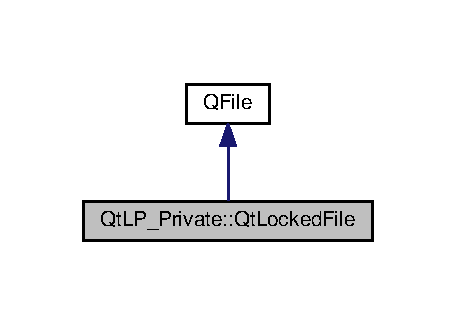
\includegraphics[width=219pt]{class_qt_l_p___private_1_1_qt_locked_file__inherit__graph}
\end{center}
\end{figure}


Collaboration diagram for Qt\+L\+P\+\_\+\+Private\+:\+:Qt\+Locked\+File\+:
\nopagebreak
\begin{figure}[H]
\begin{center}
\leavevmode
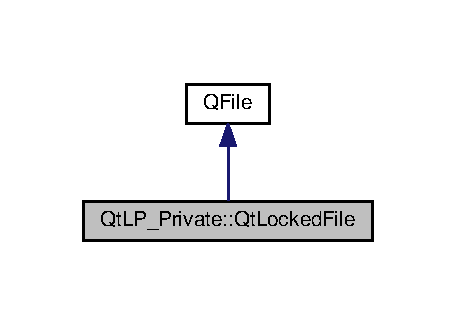
\includegraphics[width=219pt]{class_qt_l_p___private_1_1_qt_locked_file__coll__graph}
\end{center}
\end{figure}
\subsection*{Public Types}
\begin{DoxyCompactItemize}
\item 
enum \hyperlink{class_qt_l_p___private_1_1_qt_locked_file_ab9a54228983e33cf1fb8dace52141f26}{Lock\+Mode} \{ {\bfseries No\+Lock} = 0, 
{\bfseries Read\+Lock}, 
{\bfseries Write\+Lock}
 \}
\end{DoxyCompactItemize}
\subsection*{Public Member Functions}
\begin{DoxyCompactItemize}
\item 
\hyperlink{class_qt_l_p___private_1_1_qt_locked_file_a69bf1d82b1ca46f97466634d8f9587aa}{Qt\+Locked\+File} ()
\item 
\hyperlink{class_qt_l_p___private_1_1_qt_locked_file_a8b7a228ae02dca4bb99743219d0cdb7b}{Qt\+Locked\+File} (const Q\+String \&name)
\item 
\hyperlink{class_qt_l_p___private_1_1_qt_locked_file_ae22e087171c094da6cfb3282e838c9d4}{$\sim$\+Qt\+Locked\+File} ()
\item 
bool \hyperlink{class_qt_l_p___private_1_1_qt_locked_file_a2e81bbaa7b1aaa83cf79284e66dbad79}{open} (Open\+Mode mode)
\item 
bool \hyperlink{class_qt_l_p___private_1_1_qt_locked_file_af7876c08254a16d00022939f2fb9a8b8}{lock} (\hyperlink{class_qt_l_p___private_1_1_qt_locked_file_ab9a54228983e33cf1fb8dace52141f26}{Lock\+Mode} mode, bool block=true)
\item 
bool \hyperlink{class_qt_l_p___private_1_1_qt_locked_file_abb4d7e6211d9e6e14afaa661818fb2bf}{unlock} ()
\item 
bool \hyperlink{class_qt_l_p___private_1_1_qt_locked_file_ac93115b12ddd6c3275a5a81a94b6c919}{is\+Locked} () const 
\item 
\hyperlink{class_qt_l_p___private_1_1_qt_locked_file_ab9a54228983e33cf1fb8dace52141f26}{Lock\+Mode} \hyperlink{class_qt_l_p___private_1_1_qt_locked_file_aabfd6fb28f249a5fb01f3965de0e41f1}{lock\+Mode} () const 
\end{DoxyCompactItemize}


\subsection{Detailed Description}
The \hyperlink{class_qt_l_p___private_1_1_qt_locked_file}{Qt\+Locked\+File} class extends Q\+File with advisory locking functions. 

A file may be locked in read or write mode. Multiple instances of {\itshape \hyperlink{class_qt_l_p___private_1_1_qt_locked_file}{Qt\+Locked\+File}}, created in multiple processes running on the same machine, may have a file locked in read mode. Exactly one instance may have it locked in write mode. A read and a write lock cannot exist simultaneously on the same file.

The file locks are advisory. This means that nothing prevents another process from manipulating a locked file using Q\+File or file system functions offered by the OS. Serialization is only guaranteed if all processes that access the file use Q\+Locked\+File. Also, while holding a lock on a file, a process must not open the same file again (through any A\+PI), or locks can be unexpectedly lost.

The lock provided by an instance of {\itshape \hyperlink{class_qt_l_p___private_1_1_qt_locked_file}{Qt\+Locked\+File}} is released whenever the program terminates. This is true even when the program crashes and no destructors are called. 

Definition at line 67 of file qtlockedfile.\+h.



\subsection{Member Enumeration Documentation}
\index{Qt\+L\+P\+\_\+\+Private\+::\+Qt\+Locked\+File@{Qt\+L\+P\+\_\+\+Private\+::\+Qt\+Locked\+File}!Lock\+Mode@{Lock\+Mode}}
\index{Lock\+Mode@{Lock\+Mode}!Qt\+L\+P\+\_\+\+Private\+::\+Qt\+Locked\+File@{Qt\+L\+P\+\_\+\+Private\+::\+Qt\+Locked\+File}}
\subsubsection[{\texorpdfstring{Lock\+Mode}{LockMode}}]{\setlength{\rightskip}{0pt plus 5cm}enum {\bf Qt\+L\+P\+\_\+\+Private\+::\+Qt\+Locked\+File\+::\+Lock\+Mode}}\hypertarget{class_qt_l_p___private_1_1_qt_locked_file_ab9a54228983e33cf1fb8dace52141f26}{}\label{class_qt_l_p___private_1_1_qt_locked_file_ab9a54228983e33cf1fb8dace52141f26}
This enum describes the available lock modes.

Read\+Lock A read lock.  Write\+Lock A write lock.  No\+Lock Neither a read lock nor a write lock. 

Definition at line 70 of file qtlockedfile.\+h.



\subsection{Constructor \& Destructor Documentation}
\index{Qt\+L\+P\+\_\+\+Private\+::\+Qt\+Locked\+File@{Qt\+L\+P\+\_\+\+Private\+::\+Qt\+Locked\+File}!Qt\+Locked\+File@{Qt\+Locked\+File}}
\index{Qt\+Locked\+File@{Qt\+Locked\+File}!Qt\+L\+P\+\_\+\+Private\+::\+Qt\+Locked\+File@{Qt\+L\+P\+\_\+\+Private\+::\+Qt\+Locked\+File}}
\subsubsection[{\texorpdfstring{Qt\+Locked\+File()}{QtLockedFile()}}]{\setlength{\rightskip}{0pt plus 5cm}Qt\+Locked\+File\+::\+Qt\+Locked\+File (
\begin{DoxyParamCaption}
{}
\end{DoxyParamCaption}
)}\hypertarget{class_qt_l_p___private_1_1_qt_locked_file_a69bf1d82b1ca46f97466634d8f9587aa}{}\label{class_qt_l_p___private_1_1_qt_locked_file_a69bf1d82b1ca46f97466634d8f9587aa}
Constructs an unlocked {\itshape \hyperlink{class_qt_l_p___private_1_1_qt_locked_file}{Qt\+Locked\+File}} object. This constructor behaves in the same way as {\itshape Q\+File\+::\+Q\+File()}.

\begin{DoxySeeAlso}{See also}
Q\+File\+::\+Q\+File() 
\end{DoxySeeAlso}


Definition at line 83 of file qtlocalpeer.\+cpp.

\index{Qt\+L\+P\+\_\+\+Private\+::\+Qt\+Locked\+File@{Qt\+L\+P\+\_\+\+Private\+::\+Qt\+Locked\+File}!Qt\+Locked\+File@{Qt\+Locked\+File}}
\index{Qt\+Locked\+File@{Qt\+Locked\+File}!Qt\+L\+P\+\_\+\+Private\+::\+Qt\+Locked\+File@{Qt\+L\+P\+\_\+\+Private\+::\+Qt\+Locked\+File}}
\subsubsection[{\texorpdfstring{Qt\+Locked\+File(const Q\+String \&name)}{QtLockedFile(const QString &name)}}]{\setlength{\rightskip}{0pt plus 5cm}Qt\+Locked\+File\+::\+Qt\+Locked\+File (
\begin{DoxyParamCaption}
\item[{const Q\+String \&}]{name}
\end{DoxyParamCaption}
)}\hypertarget{class_qt_l_p___private_1_1_qt_locked_file_a8b7a228ae02dca4bb99743219d0cdb7b}{}\label{class_qt_l_p___private_1_1_qt_locked_file_a8b7a228ae02dca4bb99743219d0cdb7b}
Constructs an unlocked \hyperlink{class_qt_l_p___private_1_1_qt_locked_file}{Qt\+Locked\+File} object with file {\itshape name}. This constructor behaves in the same way as {\itshape Q\+File\+::\+Q\+File}(const Q\+String\&).

\begin{DoxySeeAlso}{See also}
Q\+File\+::\+Q\+File() 
\end{DoxySeeAlso}


Definition at line 100 of file qtlocalpeer.\+cpp.

\index{Qt\+L\+P\+\_\+\+Private\+::\+Qt\+Locked\+File@{Qt\+L\+P\+\_\+\+Private\+::\+Qt\+Locked\+File}!````~Qt\+Locked\+File@{$\sim$\+Qt\+Locked\+File}}
\index{````~Qt\+Locked\+File@{$\sim$\+Qt\+Locked\+File}!Qt\+L\+P\+\_\+\+Private\+::\+Qt\+Locked\+File@{Qt\+L\+P\+\_\+\+Private\+::\+Qt\+Locked\+File}}
\subsubsection[{\texorpdfstring{$\sim$\+Qt\+Locked\+File()}{~QtLockedFile()}}]{\setlength{\rightskip}{0pt plus 5cm}Qt\+Locked\+File\+::$\sim$\+Qt\+Locked\+File (
\begin{DoxyParamCaption}
{}
\end{DoxyParamCaption}
)}\hypertarget{class_qt_l_p___private_1_1_qt_locked_file_ae22e087171c094da6cfb3282e838c9d4}{}\label{class_qt_l_p___private_1_1_qt_locked_file_ae22e087171c094da6cfb3282e838c9d4}
Destroys the {\itshape \hyperlink{class_qt_l_p___private_1_1_qt_locked_file}{Qt\+Locked\+File}} object. If any locks were held, they are released. 

Definition at line 110 of file qtlocalpeer.\+cpp.



\subsection{Member Function Documentation}
\index{Qt\+L\+P\+\_\+\+Private\+::\+Qt\+Locked\+File@{Qt\+L\+P\+\_\+\+Private\+::\+Qt\+Locked\+File}!is\+Locked@{is\+Locked}}
\index{is\+Locked@{is\+Locked}!Qt\+L\+P\+\_\+\+Private\+::\+Qt\+Locked\+File@{Qt\+L\+P\+\_\+\+Private\+::\+Qt\+Locked\+File}}
\subsubsection[{\texorpdfstring{is\+Locked() const }{isLocked() const }}]{\setlength{\rightskip}{0pt plus 5cm}bool Qt\+Locked\+File\+::is\+Locked (
\begin{DoxyParamCaption}
{}
\end{DoxyParamCaption}
) const}\hypertarget{class_qt_l_p___private_1_1_qt_locked_file_ac93115b12ddd6c3275a5a81a94b6c919}{}\label{class_qt_l_p___private_1_1_qt_locked_file_ac93115b12ddd6c3275a5a81a94b6c919}
Returns {\itshape true} if this object has a in read or write lock; otherwise returns {\itshape false}.

\begin{DoxySeeAlso}{See also}
\hyperlink{class_qt_l_p___private_1_1_qt_locked_file_aabfd6fb28f249a5fb01f3965de0e41f1}{lock\+Mode()} 
\end{DoxySeeAlso}


Definition at line 138 of file qtlocalpeer.\+cpp.

\index{Qt\+L\+P\+\_\+\+Private\+::\+Qt\+Locked\+File@{Qt\+L\+P\+\_\+\+Private\+::\+Qt\+Locked\+File}!lock@{lock}}
\index{lock@{lock}!Qt\+L\+P\+\_\+\+Private\+::\+Qt\+Locked\+File@{Qt\+L\+P\+\_\+\+Private\+::\+Qt\+Locked\+File}}
\subsubsection[{\texorpdfstring{lock(\+Lock\+Mode mode, bool block=true)}{lock(LockMode mode, bool block=true)}}]{\setlength{\rightskip}{0pt plus 5cm}bool Qt\+Locked\+File\+::lock (
\begin{DoxyParamCaption}
\item[{{\bf Lock\+Mode}}]{mode, }
\item[{bool}]{block = {\ttfamily true}}
\end{DoxyParamCaption}
)}\hypertarget{class_qt_l_p___private_1_1_qt_locked_file_af7876c08254a16d00022939f2fb9a8b8}{}\label{class_qt_l_p___private_1_1_qt_locked_file_af7876c08254a16d00022939f2fb9a8b8}
Obtains a lock of type {\itshape mode}. The file must be opened before it can be locked.

If {\itshape block} is true, this function will block until the lock is aquired. If {\itshape block} is false, this function returns {\itshape false} immediately if the lock cannot be aquired.

If this object already has a lock of type {\itshape mode}, this function returns {\itshape true} immediately. If this object has a lock of a different type than {\itshape mode}, the lock is first released and then a new lock is obtained.

This function returns {\itshape true} if, after it executes, the file is locked by this object, and {\itshape false} otherwise.

\begin{DoxySeeAlso}{See also}
\hyperlink{class_qt_l_p___private_1_1_qt_locked_file_abb4d7e6211d9e6e14afaa661818fb2bf}{unlock()}, \hyperlink{class_qt_l_p___private_1_1_qt_locked_file_ac93115b12ddd6c3275a5a81a94b6c919}{is\+Locked()}, \hyperlink{class_qt_l_p___private_1_1_qt_locked_file_aabfd6fb28f249a5fb01f3965de0e41f1}{lock\+Mode()} 
\end{DoxySeeAlso}


Definition at line 48 of file qtlocalpeer.\+cpp.

\index{Qt\+L\+P\+\_\+\+Private\+::\+Qt\+Locked\+File@{Qt\+L\+P\+\_\+\+Private\+::\+Qt\+Locked\+File}!lock\+Mode@{lock\+Mode}}
\index{lock\+Mode@{lock\+Mode}!Qt\+L\+P\+\_\+\+Private\+::\+Qt\+Locked\+File@{Qt\+L\+P\+\_\+\+Private\+::\+Qt\+Locked\+File}}
\subsubsection[{\texorpdfstring{lock\+Mode() const }{lockMode() const }}]{\setlength{\rightskip}{0pt plus 5cm}{\bf Qt\+Locked\+File\+::\+Lock\+Mode} Qt\+Locked\+File\+::lock\+Mode (
\begin{DoxyParamCaption}
{}
\end{DoxyParamCaption}
) const}\hypertarget{class_qt_l_p___private_1_1_qt_locked_file_aabfd6fb28f249a5fb01f3965de0e41f1}{}\label{class_qt_l_p___private_1_1_qt_locked_file_aabfd6fb28f249a5fb01f3965de0e41f1}
Returns the type of lock currently held by this object, or {\itshape Qt\+Locked\+File\+::\+No\+Lock}.

\begin{DoxySeeAlso}{See also}
\hyperlink{class_qt_l_p___private_1_1_qt_locked_file_ac93115b12ddd6c3275a5a81a94b6c919}{is\+Locked()} 
\end{DoxySeeAlso}


Definition at line 149 of file qtlocalpeer.\+cpp.

\index{Qt\+L\+P\+\_\+\+Private\+::\+Qt\+Locked\+File@{Qt\+L\+P\+\_\+\+Private\+::\+Qt\+Locked\+File}!open@{open}}
\index{open@{open}!Qt\+L\+P\+\_\+\+Private\+::\+Qt\+Locked\+File@{Qt\+L\+P\+\_\+\+Private\+::\+Qt\+Locked\+File}}
\subsubsection[{\texorpdfstring{open(\+Open\+Mode mode)}{open(OpenMode mode)}}]{\setlength{\rightskip}{0pt plus 5cm}bool Qt\+Locked\+File\+::open (
\begin{DoxyParamCaption}
\item[{Open\+Mode}]{mode}
\end{DoxyParamCaption}
)}\hypertarget{class_qt_l_p___private_1_1_qt_locked_file_a2e81bbaa7b1aaa83cf79284e66dbad79}{}\label{class_qt_l_p___private_1_1_qt_locked_file_a2e81bbaa7b1aaa83cf79284e66dbad79}
Opens the file in Open\+Mode {\itshape mode}.

This is identical to Q\+File\+::open(), with the one exception that the Truncate mode flag is disallowed. Truncation would conflict with the advisory file locking, since the file would be modified before the write lock is obtained. If truncation is required, use resize(0) after obtaining the write lock.

Returns true if successful; otherwise false.

\begin{DoxySeeAlso}{See also}
Q\+File\+::open(), Q\+File\+::resize() 
\end{DoxySeeAlso}


Definition at line 123 of file qtlocalpeer.\+cpp.

\index{Qt\+L\+P\+\_\+\+Private\+::\+Qt\+Locked\+File@{Qt\+L\+P\+\_\+\+Private\+::\+Qt\+Locked\+File}!unlock@{unlock}}
\index{unlock@{unlock}!Qt\+L\+P\+\_\+\+Private\+::\+Qt\+Locked\+File@{Qt\+L\+P\+\_\+\+Private\+::\+Qt\+Locked\+File}}
\subsubsection[{\texorpdfstring{unlock()}{unlock()}}]{\setlength{\rightskip}{0pt plus 5cm}bool Qt\+Locked\+File\+::unlock (
\begin{DoxyParamCaption}
{}
\end{DoxyParamCaption}
)}\hypertarget{class_qt_l_p___private_1_1_qt_locked_file_abb4d7e6211d9e6e14afaa661818fb2bf}{}\label{class_qt_l_p___private_1_1_qt_locked_file_abb4d7e6211d9e6e14afaa661818fb2bf}
Releases a lock.

If the object has no lock, this function returns immediately.

This function returns {\itshape true} if, after it executes, the file is not locked by this object, and {\itshape false} otherwise.

\begin{DoxySeeAlso}{See also}
\hyperlink{class_qt_l_p___private_1_1_qt_locked_file_af7876c08254a16d00022939f2fb9a8b8}{lock()}, \hyperlink{class_qt_l_p___private_1_1_qt_locked_file_ac93115b12ddd6c3275a5a81a94b6c919}{is\+Locked()}, \hyperlink{class_qt_l_p___private_1_1_qt_locked_file_aabfd6fb28f249a5fb01f3965de0e41f1}{lock\+Mode()} 
\end{DoxySeeAlso}


Definition at line 84 of file qtlocalpeer.\+cpp.



The documentation for this class was generated from the following files\+:\begin{DoxyCompactItemize}
\item 
libs/\+Qt\+Solutions/\+Qt\+Single\+Application\+\_\+\+Core/src/qtlockedfile.\+h\item 
libs/\+Qt\+Solutions/\+Qt\+Single\+Application\+\_\+\+Core/src/qtlocalpeer.\+cpp\item 
libs/\+Qt\+Solutions/\+Qt\+Single\+Application\+\_\+\+Core/src/qtlockedfile.\+cpp\item 
libs/\+Qt\+Solutions/\+Qt\+Single\+Application\+\_\+\+Core/src/qtlockedfile\+\_\+unix.\+cpp\item 
libs/\+Qt\+Solutions/\+Qt\+Single\+Application\+\_\+\+Core/src/qtlockedfile\+\_\+win.\+cpp\end{DoxyCompactItemize}

\hypertarget{class_mdt_1_1_deploy_utils_1_1_qt_module_list}{}\section{Mdt\+:\+:Deploy\+Utils\+:\+:Qt\+Module\+List Class Reference}
\label{class_mdt_1_1_deploy_utils_1_1_qt_module_list}\index{Mdt\+::\+Deploy\+Utils\+::\+Qt\+Module\+List@{Mdt\+::\+Deploy\+Utils\+::\+Qt\+Module\+List}}


List of Qt\+Module.  




{\ttfamily \#include $<$Qt\+Module\+List.\+h$>$}

\subsection*{Public Types}
\begin{DoxyCompactItemize}
\item 
using \hyperlink{class_mdt_1_1_deploy_utils_1_1_qt_module_list_ad6f5d3797918d10ffcce59cf37fcd86f}{const\+\_\+iterator} = Q\+Vector$<$ \hyperlink{namespace_mdt_1_1_deploy_utils_af64a196dd2a56ed4930253e7fb4ed591}{Qt\+Module} $>$\+::\hyperlink{class_mdt_1_1_deploy_utils_1_1_qt_module_list_ad6f5d3797918d10ffcce59cf37fcd86f}{const\+\_\+iterator}\hypertarget{class_mdt_1_1_deploy_utils_1_1_qt_module_list_ad6f5d3797918d10ffcce59cf37fcd86f}{}\label{class_mdt_1_1_deploy_utils_1_1_qt_module_list_ad6f5d3797918d10ffcce59cf37fcd86f}

\begin{DoxyCompactList}\small\item\em S\+T\+L-\/style const iterator. \end{DoxyCompactList}\end{DoxyCompactItemize}
\subsection*{Public Member Functions}
\begin{DoxyCompactItemize}
\item 
\hyperlink{class_mdt_1_1_deploy_utils_1_1_qt_module_list_ab23ea2c60a6bf96708beb5c383b35436}{Qt\+Module\+List} ()=default\hypertarget{class_mdt_1_1_deploy_utils_1_1_qt_module_list_ab23ea2c60a6bf96708beb5c383b35436}{}\label{class_mdt_1_1_deploy_utils_1_1_qt_module_list_ab23ea2c60a6bf96708beb5c383b35436}

\begin{DoxyCompactList}\small\item\em Construct a empty module list. \end{DoxyCompactList}\item 
\hyperlink{class_mdt_1_1_deploy_utils_1_1_qt_module_list_a891a99d6bb1c71d110f5efaba0996d95}{Qt\+Module\+List} (std\+::initializer\+\_\+list$<$ \hyperlink{namespace_mdt_1_1_deploy_utils_af64a196dd2a56ed4930253e7fb4ed591}{Qt\+Module} $>$ list)\hypertarget{class_mdt_1_1_deploy_utils_1_1_qt_module_list_a891a99d6bb1c71d110f5efaba0996d95}{}\label{class_mdt_1_1_deploy_utils_1_1_qt_module_list_a891a99d6bb1c71d110f5efaba0996d95}

\begin{DoxyCompactList}\small\item\em Construct a module list from {\itshape list}. \end{DoxyCompactList}\item 
\hyperlink{class_mdt_1_1_deploy_utils_1_1_qt_module_list_a56486fa00efe046b3987b4d414af2806}{Qt\+Module\+List} (const \hyperlink{class_mdt_1_1_deploy_utils_1_1_qt_module_list}{Qt\+Module\+List} \&)=default\hypertarget{class_mdt_1_1_deploy_utils_1_1_qt_module_list_a56486fa00efe046b3987b4d414af2806}{}\label{class_mdt_1_1_deploy_utils_1_1_qt_module_list_a56486fa00efe046b3987b4d414af2806}

\begin{DoxyCompactList}\small\item\em Copy construct a module list from a other. \end{DoxyCompactList}\item 
\hyperlink{class_mdt_1_1_deploy_utils_1_1_qt_module_list}{Qt\+Module\+List} \& \hyperlink{class_mdt_1_1_deploy_utils_1_1_qt_module_list_acf58410a8bb13fb81e8aacbddc4ffec6}{operator=} (const \hyperlink{class_mdt_1_1_deploy_utils_1_1_qt_module_list}{Qt\+Module\+List} \&)=default\hypertarget{class_mdt_1_1_deploy_utils_1_1_qt_module_list_acf58410a8bb13fb81e8aacbddc4ffec6}{}\label{class_mdt_1_1_deploy_utils_1_1_qt_module_list_acf58410a8bb13fb81e8aacbddc4ffec6}

\begin{DoxyCompactList}\small\item\em Assign a module list to this one by copy. \end{DoxyCompactList}\item 
\hyperlink{class_mdt_1_1_deploy_utils_1_1_qt_module_list_a0b3220a68573bed2411c497b505623d4}{Qt\+Module\+List} (\hyperlink{class_mdt_1_1_deploy_utils_1_1_qt_module_list}{Qt\+Module\+List} \&\&)=default\hypertarget{class_mdt_1_1_deploy_utils_1_1_qt_module_list_a0b3220a68573bed2411c497b505623d4}{}\label{class_mdt_1_1_deploy_utils_1_1_qt_module_list_a0b3220a68573bed2411c497b505623d4}

\begin{DoxyCompactList}\small\item\em Move construct a module list from a other. \end{DoxyCompactList}\item 
\hyperlink{class_mdt_1_1_deploy_utils_1_1_qt_module_list}{Qt\+Module\+List} \& \hyperlink{class_mdt_1_1_deploy_utils_1_1_qt_module_list_ab2b5bb8309201a1e5301e595adfbc410}{operator=} (\hyperlink{class_mdt_1_1_deploy_utils_1_1_qt_module_list}{Qt\+Module\+List} \&\&)=default\hypertarget{class_mdt_1_1_deploy_utils_1_1_qt_module_list_ab2b5bb8309201a1e5301e595adfbc410}{}\label{class_mdt_1_1_deploy_utils_1_1_qt_module_list_ab2b5bb8309201a1e5301e595adfbc410}

\begin{DoxyCompactList}\small\item\em Assign a module list to this one by move. \end{DoxyCompactList}\item 
int \hyperlink{class_mdt_1_1_deploy_utils_1_1_qt_module_list_aa7faa888e1f35bbcb0d7eedd99949b3c}{count} () const \hypertarget{class_mdt_1_1_deploy_utils_1_1_qt_module_list_aa7faa888e1f35bbcb0d7eedd99949b3c}{}\label{class_mdt_1_1_deploy_utils_1_1_qt_module_list_aa7faa888e1f35bbcb0d7eedd99949b3c}

\begin{DoxyCompactList}\small\item\em Get count of modules in this list. \end{DoxyCompactList}\item 
void \hyperlink{class_mdt_1_1_deploy_utils_1_1_qt_module_list_a70e3eb92aadf3192bb143b09c02b5f4e}{add\+Module} (\hyperlink{namespace_mdt_1_1_deploy_utils_af64a196dd2a56ed4930253e7fb4ed591}{Qt\+Module} module)
\begin{DoxyCompactList}\small\item\em Add a modules to this list. \end{DoxyCompactList}\item 
\hyperlink{namespace_mdt_1_1_deploy_utils_af64a196dd2a56ed4930253e7fb4ed591}{Qt\+Module} \hyperlink{class_mdt_1_1_deploy_utils_1_1_qt_module_list_a4efff06b2cc4dd3001ffdc64ef1adab7}{at} (int index) const 
\begin{DoxyCompactList}\small\item\em Get module at index. \end{DoxyCompactList}\item 
void \hyperlink{class_mdt_1_1_deploy_utils_1_1_qt_module_list_ad35b7ca2a64b82f63e878875ec8a6a72}{clear} ()\hypertarget{class_mdt_1_1_deploy_utils_1_1_qt_module_list_ad35b7ca2a64b82f63e878875ec8a6a72}{}\label{class_mdt_1_1_deploy_utils_1_1_qt_module_list_ad35b7ca2a64b82f63e878875ec8a6a72}

\begin{DoxyCompactList}\small\item\em Clear this list. \end{DoxyCompactList}\item 
\hyperlink{class_mdt_1_1_deploy_utils_1_1_qt_module_list_ad6f5d3797918d10ffcce59cf37fcd86f}{const\+\_\+iterator} \hyperlink{class_mdt_1_1_deploy_utils_1_1_qt_module_list_aace993f55fee17ebe537d43d385b525c}{begin} () const \hypertarget{class_mdt_1_1_deploy_utils_1_1_qt_module_list_aace993f55fee17ebe537d43d385b525c}{}\label{class_mdt_1_1_deploy_utils_1_1_qt_module_list_aace993f55fee17ebe537d43d385b525c}

\begin{DoxyCompactList}\small\item\em Returns a const S\+T\+L-\/style iterator pointing to the first item in the list. \end{DoxyCompactList}\item 
\hyperlink{class_mdt_1_1_deploy_utils_1_1_qt_module_list_ad6f5d3797918d10ffcce59cf37fcd86f}{const\+\_\+iterator} \hyperlink{class_mdt_1_1_deploy_utils_1_1_qt_module_list_af6d4d9209eeb796785e9e15eaacc141e}{cbegin} () const \hypertarget{class_mdt_1_1_deploy_utils_1_1_qt_module_list_af6d4d9209eeb796785e9e15eaacc141e}{}\label{class_mdt_1_1_deploy_utils_1_1_qt_module_list_af6d4d9209eeb796785e9e15eaacc141e}

\begin{DoxyCompactList}\small\item\em Returns a const S\+T\+L-\/style iterator pointing to the first item in the list. \end{DoxyCompactList}\item 
\hyperlink{class_mdt_1_1_deploy_utils_1_1_qt_module_list_ad6f5d3797918d10ffcce59cf37fcd86f}{const\+\_\+iterator} \hyperlink{class_mdt_1_1_deploy_utils_1_1_qt_module_list_ae6eb25e9f98e70ccd85a763d4ba188fd}{end} () const \hypertarget{class_mdt_1_1_deploy_utils_1_1_qt_module_list_ae6eb25e9f98e70ccd85a763d4ba188fd}{}\label{class_mdt_1_1_deploy_utils_1_1_qt_module_list_ae6eb25e9f98e70ccd85a763d4ba188fd}

\begin{DoxyCompactList}\small\item\em Returns a const S\+T\+L-\/style iterator pointing to the last item in the list. \end{DoxyCompactList}\item 
\hyperlink{class_mdt_1_1_deploy_utils_1_1_qt_module_list_ad6f5d3797918d10ffcce59cf37fcd86f}{const\+\_\+iterator} \hyperlink{class_mdt_1_1_deploy_utils_1_1_qt_module_list_ac6794cb4cc68f4218cd8b71c92f09479}{cend} () const \hypertarget{class_mdt_1_1_deploy_utils_1_1_qt_module_list_ac6794cb4cc68f4218cd8b71c92f09479}{}\label{class_mdt_1_1_deploy_utils_1_1_qt_module_list_ac6794cb4cc68f4218cd8b71c92f09479}

\begin{DoxyCompactList}\small\item\em Returns a const S\+T\+L-\/style iterator pointing to the last item in the list. \end{DoxyCompactList}\end{DoxyCompactItemize}


\subsection{Detailed Description}
List of Qt\+Module. 

Definition at line 34 of file Qt\+Module\+List.\+h.



\subsection{Member Function Documentation}
\index{Mdt\+::\+Deploy\+Utils\+::\+Qt\+Module\+List@{Mdt\+::\+Deploy\+Utils\+::\+Qt\+Module\+List}!add\+Module@{add\+Module}}
\index{add\+Module@{add\+Module}!Mdt\+::\+Deploy\+Utils\+::\+Qt\+Module\+List@{Mdt\+::\+Deploy\+Utils\+::\+Qt\+Module\+List}}
\subsubsection[{\texorpdfstring{add\+Module(\+Qt\+Module module)}{addModule(QtModule module)}}]{\setlength{\rightskip}{0pt plus 5cm}void Mdt\+::\+Deploy\+Utils\+::\+Qt\+Module\+List\+::add\+Module (
\begin{DoxyParamCaption}
\item[{{\bf Qt\+Module}}]{module}
\end{DoxyParamCaption}
)}\hypertarget{class_mdt_1_1_deploy_utils_1_1_qt_module_list_a70e3eb92aadf3192bb143b09c02b5f4e}{}\label{class_mdt_1_1_deploy_utils_1_1_qt_module_list_a70e3eb92aadf3192bb143b09c02b5f4e}


Add a modules to this list. 

If {\itshape module} allready exists, it will not be added. \hyperlink{namespace_mdt_1_1_deploy_utils_a998c3ae583084b7cac9e9a71b9e1ac32a88183b946cc5f0e8c96b2e66e1c74a7e}{Qt\+Module\+::\+Unknown} will also not be added. 

Definition at line 33 of file Qt\+Module\+List.\+cpp.

\index{Mdt\+::\+Deploy\+Utils\+::\+Qt\+Module\+List@{Mdt\+::\+Deploy\+Utils\+::\+Qt\+Module\+List}!at@{at}}
\index{at@{at}!Mdt\+::\+Deploy\+Utils\+::\+Qt\+Module\+List@{Mdt\+::\+Deploy\+Utils\+::\+Qt\+Module\+List}}
\subsubsection[{\texorpdfstring{at(int index) const }{at(int index) const }}]{\setlength{\rightskip}{0pt plus 5cm}{\bf Qt\+Module} Mdt\+::\+Deploy\+Utils\+::\+Qt\+Module\+List\+::at (
\begin{DoxyParamCaption}
\item[{int}]{index}
\end{DoxyParamCaption}
) const\hspace{0.3cm}{\ttfamily [inline]}}\hypertarget{class_mdt_1_1_deploy_utils_1_1_qt_module_list_a4efff06b2cc4dd3001ffdc64ef1adab7}{}\label{class_mdt_1_1_deploy_utils_1_1_qt_module_list_a4efff06b2cc4dd3001ffdc64ef1adab7}


Get module at index. 

\begin{DoxyPrecond}{Precondition}
{\itshape index} must be in valid range (0 $>$= index $<$ \hyperlink{class_mdt_1_1_deploy_utils_1_1_qt_module_list_aa7faa888e1f35bbcb0d7eedd99949b3c}{count()}) 
\end{DoxyPrecond}


Definition at line 85 of file Qt\+Module\+List.\+h.



The documentation for this class was generated from the following files\+:\begin{DoxyCompactItemize}
\item 
libs/\+Deploy\+Utils\+\_\+\+Core/src/\+Mdt/\+Deploy\+Utils/Qt\+Module\+List.\+h\item 
libs/\+Deploy\+Utils\+\_\+\+Core/src/\+Mdt/\+Deploy\+Utils/Qt\+Module\+List.\+cpp\end{DoxyCompactItemize}

\hypertarget{class_qt_single_application}{}\section{Qt\+Single\+Application Class Reference}
\label{class_qt_single_application}\index{Qt\+Single\+Application@{Qt\+Single\+Application}}


The \hyperlink{class_qt_single_application}{Qt\+Single\+Application} class provides an A\+PI to detect and communicate with running instances of an application.  




{\ttfamily \#include $<$qtsingleapplication.\+h$>$}



Inheritance diagram for Qt\+Single\+Application\+:
\nopagebreak
\begin{figure}[H]
\begin{center}
\leavevmode
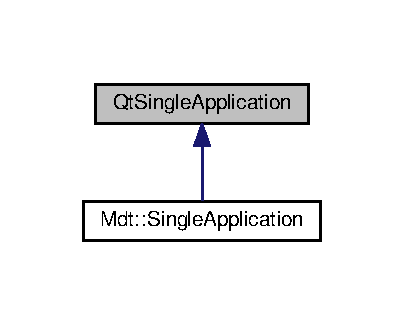
\includegraphics[width=194pt]{class_qt_single_application__inherit__graph}
\end{center}
\end{figure}
\subsection*{Public Slots}
\begin{DoxyCompactItemize}
\item 
bool \hyperlink{class_qt_single_application_a0e2f3900f0290913c738ec6b4b959922}{send\+Message} (const Q\+String \&message, int timeout=5000)
\item 
void \hyperlink{class_qt_single_application_a0881b32c76132b499f3180064006abc1}{activate\+Window} ()
\end{DoxyCompactItemize}
\subsection*{Signals}
\begin{DoxyCompactItemize}
\item 
void \hyperlink{class_qt_single_application_a69340cef3d26d026e11424930e5a5866}{message\+Received} (const Q\+String \&message)
\end{DoxyCompactItemize}
\subsection*{Public Member Functions}
\begin{DoxyCompactItemize}
\item 
\hyperlink{class_qt_single_application_afe5e96d236e42949e65669eca282acbd}{Qt\+Single\+Application} (int \&argc, char $\ast$$\ast$argv, bool G\+U\+Ienabled=true)
\item 
\hyperlink{class_qt_single_application_a746192779985e28f22fd17766884518e}{Qt\+Single\+Application} (const Q\+String \&\hyperlink{class_qt_single_application_affd094410862f30fce83afcba3457b19}{id}, int \&argc, char $\ast$$\ast$argv)
\item 
\hyperlink{class_qt_single_application_adcb7a28eec3eef34c6474fb419509895}{Qt\+Single\+Application} (int \&argc, char $\ast$$\ast$argv, Type type)
\item 
bool \hyperlink{class_qt_single_application_aa9f0e6e4f18ac79bbb7a955cd860894d}{is\+Running} ()
\item 
Q\+String \hyperlink{class_qt_single_application_affd094410862f30fce83afcba3457b19}{id} () const 
\item 
void \hyperlink{class_qt_single_application_acb5347f6dc6822dbe4d6a78804043528}{set\+Activation\+Window} (Q\+Widget $\ast$aw, bool activate\+On\+Message=true)
\item 
Q\+Widget $\ast$ \hyperlink{class_qt_single_application_a1e6be5adba2282fcfe547596b2aee18a}{activation\+Window} () const 
\item 
void \hyperlink{class_qt_single_application_a622807c60657c1a1fadec15ea5903b47}{initialize} (bool dummy=true)
\end{DoxyCompactItemize}


\subsection{Detailed Description}
The \hyperlink{class_qt_single_application}{Qt\+Single\+Application} class provides an A\+PI to detect and communicate with running instances of an application. 

This class allows you to create applications where only one instance should be running at a time. I.\+e., if the user tries to launch another instance, the already running instance will be activated instead. Another usecase is a client-\/server system, where the first started instance will assume the role of server, and the later instances will act as clients of that server.

By default, the full path of the executable file is used to determine whether two processes are instances of the same application. You can also provide an explicit identifier string that will be compared instead.

The application should create the \hyperlink{class_qt_single_application}{Qt\+Single\+Application} object early in the startup phase, and call \hyperlink{class_qt_single_application_aa9f0e6e4f18ac79bbb7a955cd860894d}{is\+Running()} to find out if another instance of this application is already running. If \hyperlink{class_qt_single_application_aa9f0e6e4f18ac79bbb7a955cd860894d}{is\+Running()} returns false, it means that no other instance is running, and this instance has assumed the role as the running instance. In this case, the application should continue with the initialization of the application user interface before entering the event loop with exec(), as normal.

The \hyperlink{class_qt_single_application_a69340cef3d26d026e11424930e5a5866}{message\+Received()} signal will be emitted when the running application receives messages from another instance of the same application. When a message is received it might be helpful to the user to raise the application so that it becomes visible. To facilitate this, \hyperlink{class_qt_single_application}{Qt\+Single\+Application} provides the \hyperlink{class_qt_single_application_acb5347f6dc6822dbe4d6a78804043528}{set\+Activation\+Window()} function and the \hyperlink{class_qt_single_application_a0881b32c76132b499f3180064006abc1}{activate\+Window()} slot.

If \hyperlink{class_qt_single_application_aa9f0e6e4f18ac79bbb7a955cd860894d}{is\+Running()} returns true, another instance is already running. It may be alerted to the fact that another instance has started by using the \hyperlink{class_qt_single_application_a0e2f3900f0290913c738ec6b4b959922}{send\+Message()} function. Also data such as startup parameters (e.\+g. the name of the file the user wanted this new instance to open) can be passed to the running instance with this function. Then, the application should terminate (or enter client mode).

If \hyperlink{class_qt_single_application_aa9f0e6e4f18ac79bbb7a955cd860894d}{is\+Running()} returns true, but \hyperlink{class_qt_single_application_a0e2f3900f0290913c738ec6b4b959922}{send\+Message()} fails, that is an indication that the running instance is frozen.

Here\textquotesingle{}s an example that shows how to convert an existing application to use \hyperlink{class_qt_single_application}{Qt\+Single\+Application}. It is very simple and does not make use of all \hyperlink{class_qt_single_application}{Qt\+Single\+Application}\textquotesingle{}s functionality (see the examples for that).


\begin{DoxyCode}
\textcolor{comment}{// Original}
\textcolor{keywordtype}{int} main(\textcolor{keywordtype}{int} argc, \textcolor{keywordtype}{char} **argv)
\{
    QApplication app(argc, argv);

    MyMainWidget mmw;
    mmw.show();
    \textcolor{keywordflow}{return} app.exec();
\}

\textcolor{comment}{// Single instance}
\textcolor{keywordtype}{int} main(\textcolor{keywordtype}{int} argc, \textcolor{keywordtype}{char} **argv)
\{
    \hyperlink{class_qt_single_application}{QtSingleApplication} app(argc, argv);

    \textcolor{keywordflow}{if} (app.isRunning())
        \textcolor{keywordflow}{return} !app.sendMessage(someDataString);

    MyMainWidget mmw;
    app.setActivationWindow(&mmw);
    mmw.show();
    \textcolor{keywordflow}{return} app.exec();
\}
\end{DoxyCode}


Once this \hyperlink{class_qt_single_application}{Qt\+Single\+Application} instance is destroyed (normally when the process exits or crashes), when the user next attempts to run the application this instance will not, of course, be encountered. The next instance to call \hyperlink{class_qt_single_application_aa9f0e6e4f18ac79bbb7a955cd860894d}{is\+Running()} or \hyperlink{class_qt_single_application_a0e2f3900f0290913c738ec6b4b959922}{send\+Message()} will assume the role as the new running instance.

For console (non-\/\+G\+UI) applications, \hyperlink{class_qt_single_core_application}{Qt\+Single\+Core\+Application} may be used instead of this class, to avoid the dependency on the Qt\+Gui library.

\begin{DoxySeeAlso}{See also}
\hyperlink{class_qt_single_core_application}{Qt\+Single\+Core\+Application} 
\end{DoxySeeAlso}


Definition at line 64 of file qtsingleapplication.\+h.



\subsection{Constructor \& Destructor Documentation}
\index{Qt\+Single\+Application@{Qt\+Single\+Application}!Qt\+Single\+Application@{Qt\+Single\+Application}}
\index{Qt\+Single\+Application@{Qt\+Single\+Application}!Qt\+Single\+Application@{Qt\+Single\+Application}}
\subsubsection[{\texorpdfstring{Qt\+Single\+Application(int \&argc, char $\ast$$\ast$argv, bool G\+U\+Ienabled=true)}{QtSingleApplication(int &argc, char **argv, bool GUIenabled=true)}}]{\setlength{\rightskip}{0pt plus 5cm}Qt\+Single\+Application\+::\+Qt\+Single\+Application (
\begin{DoxyParamCaption}
\item[{int \&}]{argc, }
\item[{char $\ast$$\ast$}]{argv, }
\item[{bool}]{G\+U\+Ienabled = {\ttfamily true}}
\end{DoxyParamCaption}
)}\hypertarget{class_qt_single_application_afe5e96d236e42949e65669eca282acbd}{}\label{class_qt_single_application_afe5e96d236e42949e65669eca282acbd}
Creates a \hyperlink{class_qt_single_application}{Qt\+Single\+Application} object. The application identifier will be Q\+Core\+Application\+::application\+File\+Path(). {\itshape argc}, {\itshape argv}, and {\itshape G\+U\+Ienabled} are passed on to the Q\+Appliation constructor.

If you are creating a console application (i.\+e. setting {\itshape G\+U\+Ienabled} to false), you may consider using \hyperlink{class_qt_single_core_application}{Qt\+Single\+Core\+Application} instead. 

Definition at line 154 of file qtsingleapplication.\+cpp.

\index{Qt\+Single\+Application@{Qt\+Single\+Application}!Qt\+Single\+Application@{Qt\+Single\+Application}}
\index{Qt\+Single\+Application@{Qt\+Single\+Application}!Qt\+Single\+Application@{Qt\+Single\+Application}}
\subsubsection[{\texorpdfstring{Qt\+Single\+Application(const Q\+String \&id, int \&argc, char $\ast$$\ast$argv)}{QtSingleApplication(const QString &id, int &argc, char **argv)}}]{\setlength{\rightskip}{0pt plus 5cm}Qt\+Single\+Application\+::\+Qt\+Single\+Application (
\begin{DoxyParamCaption}
\item[{const Q\+String \&}]{app\+Id, }
\item[{int \&}]{argc, }
\item[{char $\ast$$\ast$}]{argv}
\end{DoxyParamCaption}
)}\hypertarget{class_qt_single_application_a746192779985e28f22fd17766884518e}{}\label{class_qt_single_application_a746192779985e28f22fd17766884518e}
Creates a \hyperlink{class_qt_single_application}{Qt\+Single\+Application} object with the application identifier {\itshape app\+Id}. {\itshape argc} and {\itshape argv} are passed on to the Q\+Appliation constructor. 

Definition at line 167 of file qtsingleapplication.\+cpp.

\index{Qt\+Single\+Application@{Qt\+Single\+Application}!Qt\+Single\+Application@{Qt\+Single\+Application}}
\index{Qt\+Single\+Application@{Qt\+Single\+Application}!Qt\+Single\+Application@{Qt\+Single\+Application}}
\subsubsection[{\texorpdfstring{Qt\+Single\+Application(int \&argc, char $\ast$$\ast$argv, Type type)}{QtSingleApplication(int &argc, char **argv, Type type)}}]{\setlength{\rightskip}{0pt plus 5cm}Qt\+Single\+Application\+::\+Qt\+Single\+Application (
\begin{DoxyParamCaption}
\item[{int \&}]{argc, }
\item[{char $\ast$$\ast$}]{argv, }
\item[{Type}]{type}
\end{DoxyParamCaption}
)}\hypertarget{class_qt_single_application_adcb7a28eec3eef34c6474fb419509895}{}\label{class_qt_single_application_adcb7a28eec3eef34c6474fb419509895}
Creates a \hyperlink{class_qt_single_application}{Qt\+Single\+Application} object. The application identifier will be Q\+Core\+Application\+::application\+File\+Path(). {\itshape argc}, {\itshape argv}, and {\itshape type} are passed on to the Q\+Appliation constructor. 

Definition at line 180 of file qtsingleapplication.\+cpp.



\subsection{Member Function Documentation}
\index{Qt\+Single\+Application@{Qt\+Single\+Application}!activate\+Window@{activate\+Window}}
\index{activate\+Window@{activate\+Window}!Qt\+Single\+Application@{Qt\+Single\+Application}}
\subsubsection[{\texorpdfstring{activate\+Window}{activateWindow}}]{\setlength{\rightskip}{0pt plus 5cm}void Qt\+Single\+Application\+::activate\+Window (
\begin{DoxyParamCaption}
{}
\end{DoxyParamCaption}
)\hspace{0.3cm}{\ttfamily [slot]}}\hypertarget{class_qt_single_application_a0881b32c76132b499f3180064006abc1}{}\label{class_qt_single_application_a0881b32c76132b499f3180064006abc1}
De-\/minimizes, raises, and activates this application\textquotesingle{}s activation window. This function does nothing if no activation window has been set.

This is a convenience function to show the user that this application instance has been activated when he has tried to start another instance.

This function should typically be called in response to the \hyperlink{class_qt_single_application_a69340cef3d26d026e11424930e5a5866}{message\+Received()} signal. By default, that will happen automatically, if an activation window has been set.

\begin{DoxySeeAlso}{See also}
\hyperlink{class_qt_single_application_acb5347f6dc6822dbe4d6a78804043528}{set\+Activation\+Window()}, \hyperlink{class_qt_single_application_a69340cef3d26d026e11424930e5a5866}{message\+Received()}, \hyperlink{class_qt_single_application_a622807c60657c1a1fadec15ea5903b47}{initialize()} 
\end{DoxySeeAlso}


Definition at line 323 of file qtsingleapplication.\+cpp.

\index{Qt\+Single\+Application@{Qt\+Single\+Application}!activation\+Window@{activation\+Window}}
\index{activation\+Window@{activation\+Window}!Qt\+Single\+Application@{Qt\+Single\+Application}}
\subsubsection[{\texorpdfstring{activation\+Window() const }{activationWindow() const }}]{\setlength{\rightskip}{0pt plus 5cm}Q\+Widget $\ast$ Qt\+Single\+Application\+::activation\+Window (
\begin{DoxyParamCaption}
{}
\end{DoxyParamCaption}
) const}\hypertarget{class_qt_single_application_a1e6be5adba2282fcfe547596b2aee18a}{}\label{class_qt_single_application_a1e6be5adba2282fcfe547596b2aee18a}
Returns the applications activation window if one has been set by calling \hyperlink{class_qt_single_application_acb5347f6dc6822dbe4d6a78804043528}{set\+Activation\+Window()}, otherwise returns 0.

\begin{DoxySeeAlso}{See also}
\hyperlink{class_qt_single_application_acb5347f6dc6822dbe4d6a78804043528}{set\+Activation\+Window()} 
\end{DoxySeeAlso}


Definition at line 303 of file qtsingleapplication.\+cpp.

\index{Qt\+Single\+Application@{Qt\+Single\+Application}!id@{id}}
\index{id@{id}!Qt\+Single\+Application@{Qt\+Single\+Application}}
\subsubsection[{\texorpdfstring{id() const }{id() const }}]{\setlength{\rightskip}{0pt plus 5cm}Q\+String Qt\+Single\+Application\+::id (
\begin{DoxyParamCaption}
{}
\end{DoxyParamCaption}
) const}\hypertarget{class_qt_single_application_affd094410862f30fce83afcba3457b19}{}\label{class_qt_single_application_affd094410862f30fce83afcba3457b19}
Returns the application identifier. Two processes with the same identifier will be regarded as instances of the same application. 

Definition at line 269 of file qtsingleapplication.\+cpp.

\index{Qt\+Single\+Application@{Qt\+Single\+Application}!initialize@{initialize}}
\index{initialize@{initialize}!Qt\+Single\+Application@{Qt\+Single\+Application}}
\subsubsection[{\texorpdfstring{initialize(bool dummy=true)}{initialize(bool dummy=true)}}]{\setlength{\rightskip}{0pt plus 5cm}void Qt\+Single\+Application\+::initialize (
\begin{DoxyParamCaption}
\item[{bool}]{dummy = {\ttfamily true}}
\end{DoxyParamCaption}
)\hspace{0.3cm}{\ttfamily [inline]}}\hypertarget{class_qt_single_application_a622807c60657c1a1fadec15ea5903b47}{}\label{class_qt_single_application_a622807c60657c1a1fadec15ea5903b47}


Definition at line 87 of file qtsingleapplication.\+h.

\index{Qt\+Single\+Application@{Qt\+Single\+Application}!is\+Running@{is\+Running}}
\index{is\+Running@{is\+Running}!Qt\+Single\+Application@{Qt\+Single\+Application}}
\subsubsection[{\texorpdfstring{is\+Running()}{isRunning()}}]{\setlength{\rightskip}{0pt plus 5cm}bool Qt\+Single\+Application\+::is\+Running (
\begin{DoxyParamCaption}
{}
\end{DoxyParamCaption}
)}\hypertarget{class_qt_single_application_aa9f0e6e4f18ac79bbb7a955cd860894d}{}\label{class_qt_single_application_aa9f0e6e4f18ac79bbb7a955cd860894d}
Returns true if another instance of this application is running; otherwise false.

This function does not find instances of this application that are being run by a different user (on Windows\+: that are running in another session).

\begin{DoxySeeAlso}{See also}
\hyperlink{class_qt_single_application_a0e2f3900f0290913c738ec6b4b959922}{send\+Message()} 
\end{DoxySeeAlso}


Definition at line 240 of file qtsingleapplication.\+cpp.

\index{Qt\+Single\+Application@{Qt\+Single\+Application}!message\+Received@{message\+Received}}
\index{message\+Received@{message\+Received}!Qt\+Single\+Application@{Qt\+Single\+Application}}
\subsubsection[{\texorpdfstring{message\+Received}{messageReceived}}]{\setlength{\rightskip}{0pt plus 5cm}void Qt\+Single\+Application\+::message\+Received (
\begin{DoxyParamCaption}
\item[{const Q\+String \&}]{message}
\end{DoxyParamCaption}
)\hspace{0.3cm}{\ttfamily [signal]}}\hypertarget{class_qt_single_application_a69340cef3d26d026e11424930e5a5866}{}\label{class_qt_single_application_a69340cef3d26d026e11424930e5a5866}
This signal is emitted when the current instance receives a {\itshape message} from another instance of this application.

\begin{DoxySeeAlso}{See also}
\hyperlink{class_qt_single_application_a0e2f3900f0290913c738ec6b4b959922}{send\+Message()}, \hyperlink{class_qt_single_application_acb5347f6dc6822dbe4d6a78804043528}{set\+Activation\+Window()}, \hyperlink{class_qt_single_application_a0881b32c76132b499f3180064006abc1}{activate\+Window()} 
\end{DoxySeeAlso}
\index{Qt\+Single\+Application@{Qt\+Single\+Application}!send\+Message@{send\+Message}}
\index{send\+Message@{send\+Message}!Qt\+Single\+Application@{Qt\+Single\+Application}}
\subsubsection[{\texorpdfstring{send\+Message}{sendMessage}}]{\setlength{\rightskip}{0pt plus 5cm}bool Qt\+Single\+Application\+::send\+Message (
\begin{DoxyParamCaption}
\item[{const Q\+String \&}]{message, }
\item[{int}]{timeout = {\ttfamily 5000}}
\end{DoxyParamCaption}
)\hspace{0.3cm}{\ttfamily [slot]}}\hypertarget{class_qt_single_application_a0e2f3900f0290913c738ec6b4b959922}{}\label{class_qt_single_application_a0e2f3900f0290913c738ec6b4b959922}
Tries to send the text {\itshape message} to the currently running instance. The \hyperlink{class_qt_single_application}{Qt\+Single\+Application} object in the running instance will emit the \hyperlink{class_qt_single_application_a69340cef3d26d026e11424930e5a5866}{message\+Received()} signal when it receives the message.

This function returns true if the message has been sent to, and processed by, the current instance. If there is no instance currently running, or if the running instance fails to process the message within {\itshape timeout} milliseconds, this function return false.

\begin{DoxySeeAlso}{See also}
\hyperlink{class_qt_single_application_aa9f0e6e4f18ac79bbb7a955cd860894d}{is\+Running()}, \hyperlink{class_qt_single_application_a69340cef3d26d026e11424930e5a5866}{message\+Received()} 
\end{DoxySeeAlso}


Definition at line 259 of file qtsingleapplication.\+cpp.

\index{Qt\+Single\+Application@{Qt\+Single\+Application}!set\+Activation\+Window@{set\+Activation\+Window}}
\index{set\+Activation\+Window@{set\+Activation\+Window}!Qt\+Single\+Application@{Qt\+Single\+Application}}
\subsubsection[{\texorpdfstring{set\+Activation\+Window(\+Q\+Widget $\ast$aw, bool activate\+On\+Message=true)}{setActivationWindow(QWidget *aw, bool activateOnMessage=true)}}]{\setlength{\rightskip}{0pt plus 5cm}void Qt\+Single\+Application\+::set\+Activation\+Window (
\begin{DoxyParamCaption}
\item[{Q\+Widget $\ast$}]{aw, }
\item[{bool}]{activate\+On\+Message = {\ttfamily true}}
\end{DoxyParamCaption}
)}\hypertarget{class_qt_single_application_acb5347f6dc6822dbe4d6a78804043528}{}\label{class_qt_single_application_acb5347f6dc6822dbe4d6a78804043528}
Sets the activation window of this application to {\itshape aw}. The activation window is the widget that will be activated by \hyperlink{class_qt_single_application_a0881b32c76132b499f3180064006abc1}{activate\+Window()}. This is typically the application\textquotesingle{}s main window.

If {\itshape activate\+On\+Message} is true (the default), the window will be activated automatically every time a message is received, just prior to the \hyperlink{class_qt_single_application_a69340cef3d26d026e11424930e5a5866}{message\+Received()} signal being emitted.

\begin{DoxySeeAlso}{See also}
\hyperlink{class_qt_single_application_a0881b32c76132b499f3180064006abc1}{activate\+Window()}, \hyperlink{class_qt_single_application_a69340cef3d26d026e11424930e5a5866}{message\+Received()} 
\end{DoxySeeAlso}


Definition at line 287 of file qtsingleapplication.\+cpp.



The documentation for this class was generated from the following files\+:\begin{DoxyCompactItemize}
\item 
libs/\+Qt\+Solutions/\+Qt\+Single\+Application\+\_\+\+Widgets/src/qtsingleapplication.\+h\item 
libs/\+Qt\+Solutions/\+Qt\+Single\+Application\+\_\+\+Widgets/src/qtsingleapplication.\+cpp\end{DoxyCompactItemize}

\hypertarget{class_qt_single_core_application}{}\section{Qt\+Single\+Core\+Application Class Reference}
\label{class_qt_single_core_application}\index{Qt\+Single\+Core\+Application@{Qt\+Single\+Core\+Application}}


A variant of the \hyperlink{class_qt_single_application}{Qt\+Single\+Application} class for non-\/\+G\+UI applications.  




{\ttfamily \#include $<$qtsinglecoreapplication.\+h$>$}



Inheritance diagram for Qt\+Single\+Core\+Application\+:\nopagebreak
\begin{figure}[H]
\begin{center}
\leavevmode
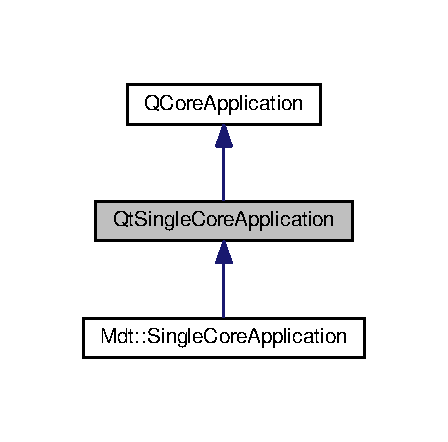
\includegraphics[width=215pt]{class_qt_single_core_application__inherit__graph}
\end{center}
\end{figure}


Collaboration diagram for Qt\+Single\+Core\+Application\+:\nopagebreak
\begin{figure}[H]
\begin{center}
\leavevmode
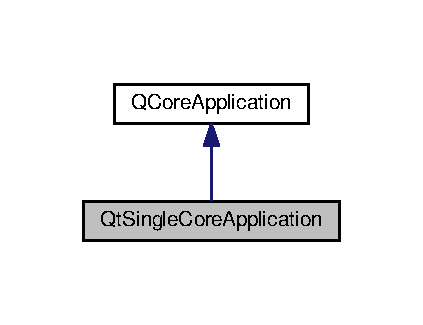
\includegraphics[width=203pt]{class_qt_single_core_application__coll__graph}
\end{center}
\end{figure}
\subsection*{Public Slots}
\begin{DoxyCompactItemize}
\item 
bool \hyperlink{class_qt_single_core_application_a07493d0807b216ca870adc6d40f856b0}{send\+Message} (const Q\+String \&message, int timeout=5000)
\end{DoxyCompactItemize}
\subsection*{Signals}
\begin{DoxyCompactItemize}
\item 
void \hyperlink{class_qt_single_core_application_a1af66a1770ff5eec8006a26a2ce42ca1}{message\+Received} (const Q\+String \&message)
\end{DoxyCompactItemize}
\subsection*{Public Member Functions}
\begin{DoxyCompactItemize}
\item 
\hyperlink{class_qt_single_core_application_a1329cb65a5706c21257f191b9d8b6548}{Qt\+Single\+Core\+Application} (int \&argc, char $\ast$$\ast$argv)
\item 
\hyperlink{class_qt_single_core_application_a2c5792a0addef95dd78b37ab55a985a7}{Qt\+Single\+Core\+Application} (const Q\+String \&\hyperlink{class_qt_single_core_application_aad587c2d4536fd153672af7ee0389478}{id}, int \&argc, char $\ast$$\ast$argv)
\item 
bool \hyperlink{class_qt_single_core_application_a419bfb7b02f0459f4d207d448bc6c876}{is\+Running} ()
\item 
Q\+String \hyperlink{class_qt_single_core_application_aad587c2d4536fd153672af7ee0389478}{id} () const 
\end{DoxyCompactItemize}


\subsection{Detailed Description}
A variant of the \hyperlink{class_qt_single_application}{Qt\+Single\+Application} class for non-\/\+G\+UI applications. 

This class is a variant of \hyperlink{class_qt_single_application}{Qt\+Single\+Application} suited for use in console (non-\/\+G\+UI) applications. It is an extension of \hyperlink{class_q_core_application}{Q\+Core\+Application} (instead of \hyperlink{class_q_application}{Q\+Application}). It does not require the Qt\+Gui library.

The A\+PI and usage is identical to \hyperlink{class_qt_single_application}{Qt\+Single\+Application}, except that functions relating to the \char`\"{}activation window\char`\"{} are not present, for obvious reasons. Please refer to the \hyperlink{class_qt_single_application}{Qt\+Single\+Application} documentation for explanation of the usage.

A \hyperlink{class_qt_single_core_application}{Qt\+Single\+Core\+Application} instance can communicate to a \hyperlink{class_qt_single_application}{Qt\+Single\+Application} instance if they share the same application id. Hence, this class can be used to create a light-\/weight command-\/line tool that sends commands to a G\+UI application.

\begin{DoxySeeAlso}{See also}
\hyperlink{class_qt_single_application}{Qt\+Single\+Application} 
\end{DoxySeeAlso}


Definition at line 48 of file qtsinglecoreapplication.\+h.



\subsection{Constructor \& Destructor Documentation}
\index{Qt\+Single\+Core\+Application@{Qt\+Single\+Core\+Application}!Qt\+Single\+Core\+Application@{Qt\+Single\+Core\+Application}}
\index{Qt\+Single\+Core\+Application@{Qt\+Single\+Core\+Application}!Qt\+Single\+Core\+Application@{Qt\+Single\+Core\+Application}}
\subsubsection[{\texorpdfstring{Qt\+Single\+Core\+Application(int \&argc, char $\ast$$\ast$argv)}{QtSingleCoreApplication(int &argc, char **argv)}}]{\setlength{\rightskip}{0pt plus 5cm}Qt\+Single\+Core\+Application\+::\+Qt\+Single\+Core\+Application (
\begin{DoxyParamCaption}
\item[{int \&}]{argc, }
\item[{char $\ast$$\ast$}]{argv}
\end{DoxyParamCaption}
)}\hypertarget{class_qt_single_core_application_a1329cb65a5706c21257f191b9d8b6548}{}\label{class_qt_single_core_application_a1329cb65a5706c21257f191b9d8b6548}
Creates a \hyperlink{class_qt_single_core_application}{Qt\+Single\+Core\+Application} object. The application identifier will be Q\+Core\+Application\+::application\+File\+Path(). {\itshape argc} and {\itshape argv} are passed on to the Q\+Core\+Appliation constructor. 

Definition at line 73 of file qtsinglecoreapplication.\+cpp.

\index{Qt\+Single\+Core\+Application@{Qt\+Single\+Core\+Application}!Qt\+Single\+Core\+Application@{Qt\+Single\+Core\+Application}}
\index{Qt\+Single\+Core\+Application@{Qt\+Single\+Core\+Application}!Qt\+Single\+Core\+Application@{Qt\+Single\+Core\+Application}}
\subsubsection[{\texorpdfstring{Qt\+Single\+Core\+Application(const Q\+String \&id, int \&argc, char $\ast$$\ast$argv)}{QtSingleCoreApplication(const QString &id, int &argc, char **argv)}}]{\setlength{\rightskip}{0pt plus 5cm}Qt\+Single\+Core\+Application\+::\+Qt\+Single\+Core\+Application (
\begin{DoxyParamCaption}
\item[{const Q\+String \&}]{app\+Id, }
\item[{int \&}]{argc, }
\item[{char $\ast$$\ast$}]{argv}
\end{DoxyParamCaption}
)}\hypertarget{class_qt_single_core_application_a2c5792a0addef95dd78b37ab55a985a7}{}\label{class_qt_single_core_application_a2c5792a0addef95dd78b37ab55a985a7}
Creates a \hyperlink{class_qt_single_core_application}{Qt\+Single\+Core\+Application} object with the application identifier {\itshape app\+Id}. {\itshape argc} and {\itshape argv} are passed on to the Q\+Core\+Appliation constructor. 

Definition at line 86 of file qtsinglecoreapplication.\+cpp.



\subsection{Member Function Documentation}
\index{Qt\+Single\+Core\+Application@{Qt\+Single\+Core\+Application}!id@{id}}
\index{id@{id}!Qt\+Single\+Core\+Application@{Qt\+Single\+Core\+Application}}
\subsubsection[{\texorpdfstring{id() const }{id() const }}]{\setlength{\rightskip}{0pt plus 5cm}Q\+String Qt\+Single\+Core\+Application\+::id (
\begin{DoxyParamCaption}
{}
\end{DoxyParamCaption}
) const}\hypertarget{class_qt_single_core_application_aad587c2d4536fd153672af7ee0389478}{}\label{class_qt_single_core_application_aad587c2d4536fd153672af7ee0389478}
Returns the application identifier. Two processes with the same identifier will be regarded as instances of the same application. 

Definition at line 136 of file qtsinglecoreapplication.\+cpp.

\index{Qt\+Single\+Core\+Application@{Qt\+Single\+Core\+Application}!is\+Running@{is\+Running}}
\index{is\+Running@{is\+Running}!Qt\+Single\+Core\+Application@{Qt\+Single\+Core\+Application}}
\subsubsection[{\texorpdfstring{is\+Running()}{isRunning()}}]{\setlength{\rightskip}{0pt plus 5cm}bool Qt\+Single\+Core\+Application\+::is\+Running (
\begin{DoxyParamCaption}
{}
\end{DoxyParamCaption}
)}\hypertarget{class_qt_single_core_application_a419bfb7b02f0459f4d207d448bc6c876}{}\label{class_qt_single_core_application_a419bfb7b02f0459f4d207d448bc6c876}
Returns true if another instance of this application is running; otherwise false.

This function does not find instances of this application that are being run by a different user (on Windows\+: that are running in another session).

\begin{DoxySeeAlso}{See also}
\hyperlink{class_qt_single_core_application_a07493d0807b216ca870adc6d40f856b0}{send\+Message()} 
\end{DoxySeeAlso}


Definition at line 105 of file qtsinglecoreapplication.\+cpp.

\index{Qt\+Single\+Core\+Application@{Qt\+Single\+Core\+Application}!message\+Received@{message\+Received}}
\index{message\+Received@{message\+Received}!Qt\+Single\+Core\+Application@{Qt\+Single\+Core\+Application}}
\subsubsection[{\texorpdfstring{message\+Received}{messageReceived}}]{\setlength{\rightskip}{0pt plus 5cm}void Qt\+Single\+Core\+Application\+::message\+Received (
\begin{DoxyParamCaption}
\item[{const Q\+String \&}]{message}
\end{DoxyParamCaption}
)\hspace{0.3cm}{\ttfamily [signal]}}\hypertarget{class_qt_single_core_application_a1af66a1770ff5eec8006a26a2ce42ca1}{}\label{class_qt_single_core_application_a1af66a1770ff5eec8006a26a2ce42ca1}
This signal is emitted when the current instance receives a {\itshape message} from another instance of this application.

\begin{DoxySeeAlso}{See also}
\hyperlink{class_qt_single_core_application_a07493d0807b216ca870adc6d40f856b0}{send\+Message()} 
\end{DoxySeeAlso}
\index{Qt\+Single\+Core\+Application@{Qt\+Single\+Core\+Application}!send\+Message@{send\+Message}}
\index{send\+Message@{send\+Message}!Qt\+Single\+Core\+Application@{Qt\+Single\+Core\+Application}}
\subsubsection[{\texorpdfstring{send\+Message}{sendMessage}}]{\setlength{\rightskip}{0pt plus 5cm}bool Qt\+Single\+Core\+Application\+::send\+Message (
\begin{DoxyParamCaption}
\item[{const Q\+String \&}]{message, }
\item[{int}]{timeout = {\ttfamily 5000}}
\end{DoxyParamCaption}
)\hspace{0.3cm}{\ttfamily [slot]}}\hypertarget{class_qt_single_core_application_a07493d0807b216ca870adc6d40f856b0}{}\label{class_qt_single_core_application_a07493d0807b216ca870adc6d40f856b0}
Tries to send the text {\itshape message} to the currently running instance. The \hyperlink{class_qt_single_core_application}{Qt\+Single\+Core\+Application} object in the running instance will emit the \hyperlink{class_qt_single_core_application_a1af66a1770ff5eec8006a26a2ce42ca1}{message\+Received()} signal when it receives the message.

This function returns true if the message has been sent to, and processed by, the current instance. If there is no instance currently running, or if the running instance fails to process the message within {\itshape timeout} milliseconds, this function return false.

\begin{DoxySeeAlso}{See also}
\hyperlink{class_qt_single_core_application_a419bfb7b02f0459f4d207d448bc6c876}{is\+Running()}, \hyperlink{class_qt_single_core_application_a1af66a1770ff5eec8006a26a2ce42ca1}{message\+Received()} 
\end{DoxySeeAlso}


Definition at line 125 of file qtsinglecoreapplication.\+cpp.



The documentation for this class was generated from the following files\+:\begin{DoxyCompactItemize}
\item 
libs/\+Qt\+Solutions/\+Qt\+Single\+Application\+\_\+\+Core/src/qtsinglecoreapplication.\+h\item 
libs/\+Qt\+Solutions/\+Qt\+Single\+Application\+\_\+\+Core/src/qtsinglecoreapplication.\+cpp\end{DoxyCompactItemize}

\hypertarget{class_mdt_1_1_plain_text_1_1_record_list_table_model}{}\section{Mdt\+:\+:Plain\+Text\+:\+:Record\+List\+Table\+Model Class Reference}
\label{class_mdt_1_1_plain_text_1_1_record_list_table_model}\index{Mdt\+::\+Plain\+Text\+::\+Record\+List\+Table\+Model@{Mdt\+::\+Plain\+Text\+::\+Record\+List\+Table\+Model}}


\hyperlink{class_mdt_1_1_plain_text_1_1_record_list_table_model}{Record\+List\+Table\+Model} is a table model to access data in a Record\+List.  




{\ttfamily \#include $<$Record\+List\+Table\+Model.\+h$>$}



Inherits Q\+Abstract\+Table\+Model.

\subsection*{Public Member Functions}
\begin{DoxyCompactItemize}
\item 
\hyperlink{class_mdt_1_1_plain_text_1_1_record_list_table_model_a8f620b5691a0a5e739dbb0fbc511dc3d}{Record\+List\+Table\+Model} (Q\+Object $\ast$parent=nullptr)
\begin{DoxyCompactList}\small\item\em Constructor. \end{DoxyCompactList}\item 
int \hyperlink{class_mdt_1_1_plain_text_1_1_record_list_table_model_a008f00dbfb47b039abaee9a23285ed91}{row\+Count} (const Q\+Model\+Index \&parent=Q\+Model\+Index()) const override
\begin{DoxyCompactList}\small\item\em Get row count. \end{DoxyCompactList}\item 
int \hyperlink{class_mdt_1_1_plain_text_1_1_record_list_table_model_a92b06d3a99bc39778893ea45c41e294d}{column\+Count} (const Q\+Model\+Index \&parent=Q\+Model\+Index()) const override
\begin{DoxyCompactList}\small\item\em Get column count. \end{DoxyCompactList}\item 
Q\+Variant \hyperlink{class_mdt_1_1_plain_text_1_1_record_list_table_model_a21f6d39cf524905be29c3668054d7cc5}{data} (const Q\+Model\+Index \&index, int role=Qt\+::\+Display\+Role) const override
\begin{DoxyCompactList}\small\item\em Get data. \end{DoxyCompactList}\item 
void \hyperlink{class_mdt_1_1_plain_text_1_1_record_list_table_model_ad12757d9766a6e1530cfeb20039dfff6}{set\+Record\+List} (const \hyperlink{class_mdt_1_1_plain_text_1_1_record_list_template}{Record\+List} \&record\+List)
\begin{DoxyCompactList}\small\item\em Set record list. \end{DoxyCompactList}\end{DoxyCompactItemize}


\subsection{Detailed Description}
\hyperlink{class_mdt_1_1_plain_text_1_1_record_list_table_model}{Record\+List\+Table\+Model} is a table model to access data in a Record\+List. 

Typical usage\+: 
\begin{DoxyCode}
\textcolor{preprocessor}{#include <Mdt/PlainText/RecordListTableModel>}
\textcolor{preprocessor}{#include <QTableView>}

\textcolor{keyword}{using namespace }\hyperlink{namespace_mdt_1_1_plain_text}{Mdt::PlainText};

\textcolor{comment}{// Build some list of records}
\hyperlink{class_mdt_1_1_plain_text_1_1_record_list_template}{RecordList} recordList = \{\{1,\textcolor{stringliteral}{"A"}\},\{2,\textcolor{stringliteral}{"B"}\}\};
\textcolor{comment}{// Setup model and view}
\hyperlink{class_mdt_1_1_plain_text_1_1_record_list_table_model}{RecordListTableModel} model;
model.\hyperlink{class_mdt_1_1_plain_text_1_1_record_list_table_model_ad12757d9766a6e1530cfeb20039dfff6}{setRecordList}(recordList);
QTableView view;
view.setModel(&model);
\end{DoxyCode}
 

Definition at line 49 of file Record\+List\+Table\+Model.\+h.



\subsection{Constructor \& Destructor Documentation}
\index{Mdt\+::\+Plain\+Text\+::\+Record\+List\+Table\+Model@{Mdt\+::\+Plain\+Text\+::\+Record\+List\+Table\+Model}!Record\+List\+Table\+Model@{Record\+List\+Table\+Model}}
\index{Record\+List\+Table\+Model@{Record\+List\+Table\+Model}!Mdt\+::\+Plain\+Text\+::\+Record\+List\+Table\+Model@{Mdt\+::\+Plain\+Text\+::\+Record\+List\+Table\+Model}}
\subsubsection[{\texorpdfstring{Record\+List\+Table\+Model(\+Q\+Object $\ast$parent=nullptr)}{RecordListTableModel(QObject *parent=nullptr)}}]{\setlength{\rightskip}{0pt plus 5cm}Mdt\+::\+Plain\+Text\+::\+Record\+List\+Table\+Model\+::\+Record\+List\+Table\+Model (
\begin{DoxyParamCaption}
\item[{Q\+Object $\ast$}]{parent = {\ttfamily nullptr}}
\end{DoxyParamCaption}
)\hspace{0.3cm}{\ttfamily [explicit]}}\hypertarget{class_mdt_1_1_plain_text_1_1_record_list_table_model_a8f620b5691a0a5e739dbb0fbc511dc3d}{}\label{class_mdt_1_1_plain_text_1_1_record_list_table_model_a8f620b5691a0a5e739dbb0fbc511dc3d}


Constructor. 



Definition at line 27 of file Record\+List\+Table\+Model.\+cpp.



\subsection{Member Function Documentation}
\index{Mdt\+::\+Plain\+Text\+::\+Record\+List\+Table\+Model@{Mdt\+::\+Plain\+Text\+::\+Record\+List\+Table\+Model}!column\+Count@{column\+Count}}
\index{column\+Count@{column\+Count}!Mdt\+::\+Plain\+Text\+::\+Record\+List\+Table\+Model@{Mdt\+::\+Plain\+Text\+::\+Record\+List\+Table\+Model}}
\subsubsection[{\texorpdfstring{column\+Count(const Q\+Model\+Index \&parent=\+Q\+Model\+Index()) const override}{columnCount(const QModelIndex &parent=QModelIndex()) const override}}]{\setlength{\rightskip}{0pt plus 5cm}int Mdt\+::\+Plain\+Text\+::\+Record\+List\+Table\+Model\+::column\+Count (
\begin{DoxyParamCaption}
\item[{const Q\+Model\+Index \&}]{parent = {\ttfamily QModelIndex()}}
\end{DoxyParamCaption}
) const\hspace{0.3cm}{\ttfamily [override]}}\hypertarget{class_mdt_1_1_plain_text_1_1_record_list_table_model_a92b06d3a99bc39778893ea45c41e294d}{}\label{class_mdt_1_1_plain_text_1_1_record_list_table_model_a92b06d3a99bc39778893ea45c41e294d}


Get column count. 



Definition at line 40 of file Record\+List\+Table\+Model.\+cpp.

\index{Mdt\+::\+Plain\+Text\+::\+Record\+List\+Table\+Model@{Mdt\+::\+Plain\+Text\+::\+Record\+List\+Table\+Model}!data@{data}}
\index{data@{data}!Mdt\+::\+Plain\+Text\+::\+Record\+List\+Table\+Model@{Mdt\+::\+Plain\+Text\+::\+Record\+List\+Table\+Model}}
\subsubsection[{\texorpdfstring{data(const Q\+Model\+Index \&index, int role=\+Qt\+::\+Display\+Role) const override}{data(const QModelIndex &index, int role=Qt::DisplayRole) const override}}]{\setlength{\rightskip}{0pt plus 5cm}Q\+Variant Mdt\+::\+Plain\+Text\+::\+Record\+List\+Table\+Model\+::data (
\begin{DoxyParamCaption}
\item[{const Q\+Model\+Index \&}]{index, }
\item[{int}]{role = {\ttfamily Qt\+:\+:DisplayRole}}
\end{DoxyParamCaption}
) const\hspace{0.3cm}{\ttfamily [override]}}\hypertarget{class_mdt_1_1_plain_text_1_1_record_list_table_model_a21f6d39cf524905be29c3668054d7cc5}{}\label{class_mdt_1_1_plain_text_1_1_record_list_table_model_a21f6d39cf524905be29c3668054d7cc5}


Get data. 



Definition at line 48 of file Record\+List\+Table\+Model.\+cpp.

\index{Mdt\+::\+Plain\+Text\+::\+Record\+List\+Table\+Model@{Mdt\+::\+Plain\+Text\+::\+Record\+List\+Table\+Model}!row\+Count@{row\+Count}}
\index{row\+Count@{row\+Count}!Mdt\+::\+Plain\+Text\+::\+Record\+List\+Table\+Model@{Mdt\+::\+Plain\+Text\+::\+Record\+List\+Table\+Model}}
\subsubsection[{\texorpdfstring{row\+Count(const Q\+Model\+Index \&parent=\+Q\+Model\+Index()) const override}{rowCount(const QModelIndex &parent=QModelIndex()) const override}}]{\setlength{\rightskip}{0pt plus 5cm}int Mdt\+::\+Plain\+Text\+::\+Record\+List\+Table\+Model\+::row\+Count (
\begin{DoxyParamCaption}
\item[{const Q\+Model\+Index \&}]{parent = {\ttfamily QModelIndex()}}
\end{DoxyParamCaption}
) const\hspace{0.3cm}{\ttfamily [override]}}\hypertarget{class_mdt_1_1_plain_text_1_1_record_list_table_model_a008f00dbfb47b039abaee9a23285ed91}{}\label{class_mdt_1_1_plain_text_1_1_record_list_table_model_a008f00dbfb47b039abaee9a23285ed91}


Get row count. 



Definition at line 32 of file Record\+List\+Table\+Model.\+cpp.

\index{Mdt\+::\+Plain\+Text\+::\+Record\+List\+Table\+Model@{Mdt\+::\+Plain\+Text\+::\+Record\+List\+Table\+Model}!set\+Record\+List@{set\+Record\+List}}
\index{set\+Record\+List@{set\+Record\+List}!Mdt\+::\+Plain\+Text\+::\+Record\+List\+Table\+Model@{Mdt\+::\+Plain\+Text\+::\+Record\+List\+Table\+Model}}
\subsubsection[{\texorpdfstring{set\+Record\+List(const Record\+List \&record\+List)}{setRecordList(const RecordList &recordList)}}]{\setlength{\rightskip}{0pt plus 5cm}void Mdt\+::\+Plain\+Text\+::\+Record\+List\+Table\+Model\+::set\+Record\+List (
\begin{DoxyParamCaption}
\item[{const {\bf Record\+List} \&}]{record\+List}
\end{DoxyParamCaption}
)}\hypertarget{class_mdt_1_1_plain_text_1_1_record_list_table_model_ad12757d9766a6e1530cfeb20039dfff6}{}\label{class_mdt_1_1_plain_text_1_1_record_list_table_model_ad12757d9766a6e1530cfeb20039dfff6}


Set record list. 

Note that setting a new record list will reset the model. 

Definition at line 65 of file Record\+List\+Table\+Model.\+cpp.



The documentation for this class was generated from the following files\+:\begin{DoxyCompactItemize}
\item 
libs/\+Plain\+Text\+\_\+\+Core/src/\+Mdt/\+Plain\+Text/Record\+List\+Table\+Model.\+h\item 
libs/\+Plain\+Text\+\_\+\+Core/src/\+Mdt/\+Plain\+Text/Record\+List\+Table\+Model.\+cpp\end{DoxyCompactItemize}

\hypertarget{class_mdt_1_1_plain_text_1_1_record_list_template}{}\section{Mdt\+:\+:Plain\+Text\+:\+:Record\+List\+Template$<$ Record\+Type, T $>$ Class Template Reference}
\label{class_mdt_1_1_plain_text_1_1_record_list_template}\index{Mdt\+::\+Plain\+Text\+::\+Record\+List\+Template$<$ Record\+Type, T $>$@{Mdt\+::\+Plain\+Text\+::\+Record\+List\+Template$<$ Record\+Type, T $>$}}


\hyperlink{class_mdt_1_1_plain_text_1_1_record_list_template}{Record\+List\+Template} is a list of \hyperlink{class_mdt_1_1_plain_text_1_1_record_template}{Record\+Template}.  




{\ttfamily \#include $<$Record\+List\+Template.\+h$>$}



Inheritance diagram for Mdt\+:\+:Plain\+Text\+:\+:Record\+List\+Template$<$ Record\+Type, T $>$\+:
\nopagebreak
\begin{figure}[H]
\begin{center}
\leavevmode
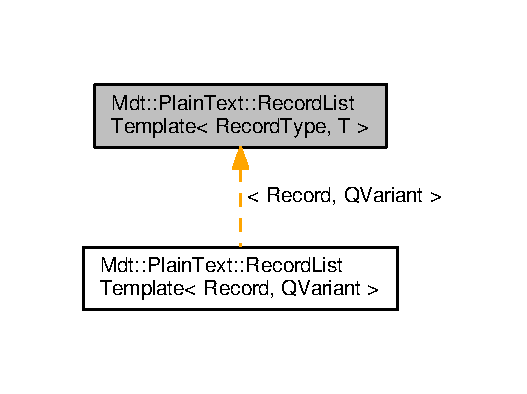
\includegraphics[width=253pt]{class_mdt_1_1_plain_text_1_1_record_list_template__inherit__graph}
\end{center}
\end{figure}
\subsection*{Public Types}
\begin{DoxyCompactItemize}
\item 
using \hyperlink{class_mdt_1_1_plain_text_1_1_record_list_template_a5b0caae56b05a38e53539cad1da8cd12}{iterator} = typename Q\+Vector$<$ Record\+Type $>$\+::\hyperlink{class_mdt_1_1_plain_text_1_1_record_list_template_a5b0caae56b05a38e53539cad1da8cd12}{iterator}
\begin{DoxyCompactList}\small\item\em S\+TL iterator. \end{DoxyCompactList}\item 
using \hyperlink{class_mdt_1_1_plain_text_1_1_record_list_template_abfba36291fe9cb605ec432ed873ce4ea}{const\+\_\+iterator} = typename Q\+Vector$<$ Record\+Type $>$\+::\hyperlink{class_mdt_1_1_plain_text_1_1_record_list_template_abfba36291fe9cb605ec432ed873ce4ea}{const\+\_\+iterator}
\begin{DoxyCompactList}\small\item\em S\+TL const iterator. \end{DoxyCompactList}\item 
using \hyperlink{class_mdt_1_1_plain_text_1_1_record_list_template_a15ca07bf051f835ce544901a06639990}{value\+\_\+type} = typename Q\+Vector$<$ Record\+Type $>$\+::\hyperlink{class_mdt_1_1_plain_text_1_1_record_list_template_a15ca07bf051f835ce544901a06639990}{value\+\_\+type}
\begin{DoxyCompactList}\small\item\em Value type for S\+TL compatibility. \end{DoxyCompactList}\item 
using \hyperlink{class_mdt_1_1_plain_text_1_1_record_list_template_a9f3af13db580a27488883003f589489f}{reference} = typename Q\+Vector$<$ Record\+Type $>$\+::\hyperlink{class_mdt_1_1_plain_text_1_1_record_list_template_a9f3af13db580a27488883003f589489f}{reference}
\begin{DoxyCompactList}\small\item\em Reference type for S\+TL compatibility. \end{DoxyCompactList}\item 
using \hyperlink{class_mdt_1_1_plain_text_1_1_record_list_template_af264f3a2efda437fd0f58cbb15209b06}{const\+\_\+reference} = typename Q\+Vector$<$ Record\+Type $>$\+::\hyperlink{class_mdt_1_1_plain_text_1_1_record_list_template_af264f3a2efda437fd0f58cbb15209b06}{const\+\_\+reference}
\begin{DoxyCompactList}\small\item\em Const reference type for S\+TL compatibility. \end{DoxyCompactList}\item 
using \hyperlink{class_mdt_1_1_plain_text_1_1_record_list_template_ac5b714fe2e3a5361f343ee1b9a49546b}{size\+\_\+type} = typename Q\+Vector$<$ Record\+Type $>$\+::\hyperlink{class_mdt_1_1_plain_text_1_1_record_list_template_ac5b714fe2e3a5361f343ee1b9a49546b}{size\+\_\+type}
\begin{DoxyCompactList}\small\item\em Size type for S\+TL compatibility. \end{DoxyCompactList}\item 
using \hyperlink{class_mdt_1_1_plain_text_1_1_record_list_template_a95aa000e23da3c55a41e4d9e81ffedbb}{pointer} = typename Q\+Vector$<$ Record\+Type $>$\+::\hyperlink{class_mdt_1_1_plain_text_1_1_record_list_template_a95aa000e23da3c55a41e4d9e81ffedbb}{pointer}
\begin{DoxyCompactList}\small\item\em Pointer type for S\+TL compatibility. \end{DoxyCompactList}\item 
using \hyperlink{class_mdt_1_1_plain_text_1_1_record_list_template_a4f7a4908afbe8ec86a57c2a9922ceed3}{const\+\_\+pointer} = typename Q\+Vector$<$ Record\+Type $>$\+::\hyperlink{class_mdt_1_1_plain_text_1_1_record_list_template_a4f7a4908afbe8ec86a57c2a9922ceed3}{const\+\_\+pointer}
\begin{DoxyCompactList}\small\item\em Const pointer type for S\+TL compatibility. \end{DoxyCompactList}\item 
using \hyperlink{class_mdt_1_1_plain_text_1_1_record_list_template_a93665d213efef18c64b3470164f8e57d}{difference\+\_\+type} = typename Q\+Vector$<$ Record\+Type $>$\+::\hyperlink{class_mdt_1_1_plain_text_1_1_record_list_template_a93665d213efef18c64b3470164f8e57d}{difference\+\_\+type}
\begin{DoxyCompactList}\small\item\em Difference type for S\+TL compatibility. \end{DoxyCompactList}\end{DoxyCompactItemize}
\subsection*{Public Member Functions}
\begin{DoxyCompactItemize}
\item 
\hyperlink{class_mdt_1_1_plain_text_1_1_record_list_template_aafe80579c379230512b75b84e199661b}{Record\+List\+Template} ()=default
\begin{DoxyCompactList}\small\item\em Construct a empty record list. \end{DoxyCompactList}\item 
\hyperlink{class_mdt_1_1_plain_text_1_1_record_list_template_a7355c51d8c8f7218b46f1dbdd65fe514}{Record\+List\+Template} (std\+::initializer\+\_\+list$<$ Record\+Type $>$ list)
\begin{DoxyCompactList}\small\item\em Construct a record list from initializer lists. \end{DoxyCompactList}\item 
\hyperlink{class_mdt_1_1_plain_text_1_1_record_list_template_a09ac82a5ab35a269fbb3bb0a28d3f4fc}{Record\+List\+Template} (const \hyperlink{class_mdt_1_1_plain_text_1_1_record_list_template}{Record\+List\+Template} \&other)=default
\begin{DoxyCompactList}\small\item\em Copy construct a record list from {\itshape other}. \end{DoxyCompactList}\item 
\hyperlink{class_mdt_1_1_plain_text_1_1_record_list_template}{Record\+List\+Template} \& \hyperlink{class_mdt_1_1_plain_text_1_1_record_list_template_adb8412269238f4ac6359716124e5cc7c}{operator=} (const \hyperlink{class_mdt_1_1_plain_text_1_1_record_list_template}{Record\+List\+Template} \&other)=default
\begin{DoxyCompactList}\small\item\em Copy assign {\itshape other} to this record list. \end{DoxyCompactList}\item 
\hyperlink{class_mdt_1_1_plain_text_1_1_record_list_template_ac0420a409eaa29f9716662faec808bb2}{Record\+List\+Template} (\hyperlink{class_mdt_1_1_plain_text_1_1_record_list_template}{Record\+List\+Template} \&\&other)=default
\begin{DoxyCompactList}\small\item\em Move construct a record list from {\itshape other}. \end{DoxyCompactList}\item 
\hyperlink{class_mdt_1_1_plain_text_1_1_record_list_template}{Record\+List\+Template} \& \hyperlink{class_mdt_1_1_plain_text_1_1_record_list_template_a323367ad799d8ec5398e56e6de9d933e}{operator=} (\hyperlink{class_mdt_1_1_plain_text_1_1_record_list_template}{Record\+List\+Template} \&\&other)=default
\begin{DoxyCompactList}\small\item\em Move assign {\itshape other} to this record list. \end{DoxyCompactList}\item 
void \hyperlink{class_mdt_1_1_plain_text_1_1_record_list_template_acf9720dd89942675131a6784277693de}{append\+Record} (const Record\+Type \&record)
\begin{DoxyCompactList}\small\item\em Append a record. \end{DoxyCompactList}\item 
void \hyperlink{class_mdt_1_1_plain_text_1_1_record_list_template_a0d87d865b6c32aa07f9f5d85a3139a8a}{push\+\_\+back} (const Record\+Type \&record)
\begin{DoxyCompactList}\small\item\em Append record to this record list. \end{DoxyCompactList}\item 
\hyperlink{class_mdt_1_1_plain_text_1_1_record_list_template_a5b0caae56b05a38e53539cad1da8cd12}{iterator} \hyperlink{class_mdt_1_1_plain_text_1_1_record_list_template_ad61ba099c68f630c7d6001fbfd6a277a}{insert} (\hyperlink{class_mdt_1_1_plain_text_1_1_record_list_template_a5b0caae56b05a38e53539cad1da8cd12}{iterator} before, const Record\+Type \&record)
\begin{DoxyCompactList}\small\item\em Insert record to this record list. \end{DoxyCompactList}\item 
bool \hyperlink{class_mdt_1_1_plain_text_1_1_record_list_template_abe112d23858a17cc597d3acebf4b1389}{is\+Empty} () const 
\begin{DoxyCompactList}\small\item\em Check if this record list is empty. \end{DoxyCompactList}\item 
int \hyperlink{class_mdt_1_1_plain_text_1_1_record_list_template_a04eb7dcdccf22e771d5012d4946cb013}{row\+Count} () const 
\begin{DoxyCompactList}\small\item\em Get row count. \end{DoxyCompactList}\item 
int \hyperlink{class_mdt_1_1_plain_text_1_1_record_list_template_a59bfaf592d639840e2ce965b11185477}{column\+Count} (int row) const 
\begin{DoxyCompactList}\small\item\em Get column count for given row. \end{DoxyCompactList}\item 
void \hyperlink{class_mdt_1_1_plain_text_1_1_record_list_template_a53a8348c93099f99a8c53426c50e958b}{set\+Data} (int row, int column, const T \&\hyperlink{class_mdt_1_1_plain_text_1_1_record_list_template_a8bccf84419669f678d3f055d89fed002}{data})
\begin{DoxyCompactList}\small\item\em Set data for given row and column. \end{DoxyCompactList}\item 
T \hyperlink{class_mdt_1_1_plain_text_1_1_record_list_template_a8bccf84419669f678d3f055d89fed002}{data} (int row, int column) const 
\begin{DoxyCompactList}\small\item\em Get data for given row and column. \end{DoxyCompactList}\item 
T \hyperlink{class_mdt_1_1_plain_text_1_1_record_list_template_ac009f422a8f6b82f3633e2629c32ca52}{value} (int row, int column) const 
\begin{DoxyCompactList}\small\item\em Get value for given row and column. \end{DoxyCompactList}\item 
void \hyperlink{class_mdt_1_1_plain_text_1_1_record_list_template_aca9f27ea6367e4753dbcc07f457547b4}{clear} ()
\begin{DoxyCompactList}\small\item\em Clear. \end{DoxyCompactList}\item 
\hyperlink{class_mdt_1_1_plain_text_1_1_record_list_template}{Record\+List\+Template} \& \hyperlink{class_mdt_1_1_plain_text_1_1_record_list_template_a9e41a19aba8a50bbeabc0e1e76dd4b42}{operator$<$$<$} (const Record\+Type \&record)
\begin{DoxyCompactList}\small\item\em Appends a row with {\itshape record} to this record list. \end{DoxyCompactList}\item 
\hyperlink{class_mdt_1_1_plain_text_1_1_record_list_template_a5b0caae56b05a38e53539cad1da8cd12}{iterator} \hyperlink{class_mdt_1_1_plain_text_1_1_record_list_template_af4f42b3785c7ddbbafd9bf3c15ead7d4}{begin} ()
\begin{DoxyCompactList}\small\item\em Get an S\+T\+L-\/style iterator pointing to the first item in the record list. \end{DoxyCompactList}\item 
\hyperlink{class_mdt_1_1_plain_text_1_1_record_list_template_a5b0caae56b05a38e53539cad1da8cd12}{iterator} \hyperlink{class_mdt_1_1_plain_text_1_1_record_list_template_accf34cd248a894d4af04510312bbdf23}{end} ()
\begin{DoxyCompactList}\small\item\em Get an S\+T\+L-\/style iterator pointing past the last item in the record list. \end{DoxyCompactList}\item 
\hyperlink{class_mdt_1_1_plain_text_1_1_record_list_template_abfba36291fe9cb605ec432ed873ce4ea}{const\+\_\+iterator} \hyperlink{class_mdt_1_1_plain_text_1_1_record_list_template_a2811685c9280d271f83bcff058658533}{begin} () const 
\begin{DoxyCompactList}\small\item\em Get an S\+T\+L-\/style const iterator pointing to the first item in the record list. \end{DoxyCompactList}\item 
\hyperlink{class_mdt_1_1_plain_text_1_1_record_list_template_abfba36291fe9cb605ec432ed873ce4ea}{const\+\_\+iterator} \hyperlink{class_mdt_1_1_plain_text_1_1_record_list_template_abaa79756cbf4ff040525344c03871f58}{end} () const 
\begin{DoxyCompactList}\small\item\em Get an S\+T\+L-\/style const iterator pointing past the last item in the record list. \end{DoxyCompactList}\item 
\hyperlink{class_mdt_1_1_plain_text_1_1_record_list_template_abfba36291fe9cb605ec432ed873ce4ea}{const\+\_\+iterator} \hyperlink{class_mdt_1_1_plain_text_1_1_record_list_template_a95499c9fa8b7bfe2f024d2d71931827e}{cbegin} () const 
\begin{DoxyCompactList}\small\item\em Get an S\+T\+L-\/style const iterator pointing to the first item in the record list. \end{DoxyCompactList}\item 
\hyperlink{class_mdt_1_1_plain_text_1_1_record_list_template_abfba36291fe9cb605ec432ed873ce4ea}{const\+\_\+iterator} \hyperlink{class_mdt_1_1_plain_text_1_1_record_list_template_adbc8ef6c14603d50d96774fd81837a6c}{cend} () const 
\begin{DoxyCompactList}\small\item\em Get an S\+T\+L-\/style const iterator pointing past the last item in the record list. \end{DoxyCompactList}\item 
\hyperlink{class_mdt_1_1_plain_text_1_1_record_list_template_a5b0caae56b05a38e53539cad1da8cd12}{iterator} \hyperlink{class_mdt_1_1_plain_text_1_1_record_list_template_a0266fea4751369b369d81933043b87a9}{erase} (\hyperlink{class_mdt_1_1_plain_text_1_1_record_list_template_a5b0caae56b05a38e53539cad1da8cd12}{iterator} \hyperlink{class_mdt_1_1_plain_text_1_1_record_list_template_af4f42b3785c7ddbbafd9bf3c15ead7d4}{begin}, \hyperlink{class_mdt_1_1_plain_text_1_1_record_list_template_a5b0caae56b05a38e53539cad1da8cd12}{iterator} \hyperlink{class_mdt_1_1_plain_text_1_1_record_list_template_accf34cd248a894d4af04510312bbdf23}{end})
\begin{DoxyCompactList}\small\item\em Removes all the items from begin up to (but not including) end. \end{DoxyCompactList}\end{DoxyCompactItemize}


\subsection{Detailed Description}
\subsubsection*{template$<$typename Record\+Type, typename T$>$\\*
class Mdt\+::\+Plain\+Text\+::\+Record\+List\+Template$<$ Record\+Type, T $>$}

\hyperlink{class_mdt_1_1_plain_text_1_1_record_list_template}{Record\+List\+Template} is a list of \hyperlink{class_mdt_1_1_plain_text_1_1_record_template}{Record\+Template}. 

\begin{DoxySeeAlso}{See also}
Record\+List 

String\+Record\+List 
\end{DoxySeeAlso}


Definition at line 35 of file Record\+List\+Template.\+h.



\subsection{Member Typedef Documentation}
\index{Mdt\+::\+Plain\+Text\+::\+Record\+List\+Template@{Mdt\+::\+Plain\+Text\+::\+Record\+List\+Template}!const\+\_\+iterator@{const\+\_\+iterator}}
\index{const\+\_\+iterator@{const\+\_\+iterator}!Mdt\+::\+Plain\+Text\+::\+Record\+List\+Template@{Mdt\+::\+Plain\+Text\+::\+Record\+List\+Template}}
\subsubsection[{\texorpdfstring{const\+\_\+iterator}{const_iterator}}]{\setlength{\rightskip}{0pt plus 5cm}template$<$typename Record\+Type, typename T$>$ using {\bf Mdt\+::\+Plain\+Text\+::\+Record\+List\+Template}$<$ Record\+Type, T $>$\+::{\bf const\+\_\+iterator} =  typename Q\+Vector$<$Record\+Type$>$\+::{\bf const\+\_\+iterator}}\hypertarget{class_mdt_1_1_plain_text_1_1_record_list_template_abfba36291fe9cb605ec432ed873ce4ea}{}\label{class_mdt_1_1_plain_text_1_1_record_list_template_abfba36291fe9cb605ec432ed873ce4ea}


S\+TL const iterator. 



Definition at line 45 of file Record\+List\+Template.\+h.

\index{Mdt\+::\+Plain\+Text\+::\+Record\+List\+Template@{Mdt\+::\+Plain\+Text\+::\+Record\+List\+Template}!const\+\_\+pointer@{const\+\_\+pointer}}
\index{const\+\_\+pointer@{const\+\_\+pointer}!Mdt\+::\+Plain\+Text\+::\+Record\+List\+Template@{Mdt\+::\+Plain\+Text\+::\+Record\+List\+Template}}
\subsubsection[{\texorpdfstring{const\+\_\+pointer}{const_pointer}}]{\setlength{\rightskip}{0pt plus 5cm}template$<$typename Record\+Type, typename T$>$ using {\bf Mdt\+::\+Plain\+Text\+::\+Record\+List\+Template}$<$ Record\+Type, T $>$\+::{\bf const\+\_\+pointer} =  typename Q\+Vector$<$Record\+Type$>$\+::{\bf const\+\_\+pointer}}\hypertarget{class_mdt_1_1_plain_text_1_1_record_list_template_a4f7a4908afbe8ec86a57c2a9922ceed3}{}\label{class_mdt_1_1_plain_text_1_1_record_list_template_a4f7a4908afbe8ec86a57c2a9922ceed3}


Const pointer type for S\+TL compatibility. 



Definition at line 69 of file Record\+List\+Template.\+h.

\index{Mdt\+::\+Plain\+Text\+::\+Record\+List\+Template@{Mdt\+::\+Plain\+Text\+::\+Record\+List\+Template}!const\+\_\+reference@{const\+\_\+reference}}
\index{const\+\_\+reference@{const\+\_\+reference}!Mdt\+::\+Plain\+Text\+::\+Record\+List\+Template@{Mdt\+::\+Plain\+Text\+::\+Record\+List\+Template}}
\subsubsection[{\texorpdfstring{const\+\_\+reference}{const_reference}}]{\setlength{\rightskip}{0pt plus 5cm}template$<$typename Record\+Type, typename T$>$ using {\bf Mdt\+::\+Plain\+Text\+::\+Record\+List\+Template}$<$ Record\+Type, T $>$\+::{\bf const\+\_\+reference} =  typename Q\+Vector$<$Record\+Type$>$\+::{\bf const\+\_\+reference}}\hypertarget{class_mdt_1_1_plain_text_1_1_record_list_template_af264f3a2efda437fd0f58cbb15209b06}{}\label{class_mdt_1_1_plain_text_1_1_record_list_template_af264f3a2efda437fd0f58cbb15209b06}


Const reference type for S\+TL compatibility. 



Definition at line 57 of file Record\+List\+Template.\+h.

\index{Mdt\+::\+Plain\+Text\+::\+Record\+List\+Template@{Mdt\+::\+Plain\+Text\+::\+Record\+List\+Template}!difference\+\_\+type@{difference\+\_\+type}}
\index{difference\+\_\+type@{difference\+\_\+type}!Mdt\+::\+Plain\+Text\+::\+Record\+List\+Template@{Mdt\+::\+Plain\+Text\+::\+Record\+List\+Template}}
\subsubsection[{\texorpdfstring{difference\+\_\+type}{difference_type}}]{\setlength{\rightskip}{0pt plus 5cm}template$<$typename Record\+Type, typename T$>$ using {\bf Mdt\+::\+Plain\+Text\+::\+Record\+List\+Template}$<$ Record\+Type, T $>$\+::{\bf difference\+\_\+type} =  typename Q\+Vector$<$Record\+Type$>$\+::{\bf difference\+\_\+type}}\hypertarget{class_mdt_1_1_plain_text_1_1_record_list_template_a93665d213efef18c64b3470164f8e57d}{}\label{class_mdt_1_1_plain_text_1_1_record_list_template_a93665d213efef18c64b3470164f8e57d}


Difference type for S\+TL compatibility. 



Definition at line 73 of file Record\+List\+Template.\+h.

\index{Mdt\+::\+Plain\+Text\+::\+Record\+List\+Template@{Mdt\+::\+Plain\+Text\+::\+Record\+List\+Template}!iterator@{iterator}}
\index{iterator@{iterator}!Mdt\+::\+Plain\+Text\+::\+Record\+List\+Template@{Mdt\+::\+Plain\+Text\+::\+Record\+List\+Template}}
\subsubsection[{\texorpdfstring{iterator}{iterator}}]{\setlength{\rightskip}{0pt plus 5cm}template$<$typename Record\+Type, typename T$>$ using {\bf Mdt\+::\+Plain\+Text\+::\+Record\+List\+Template}$<$ Record\+Type, T $>$\+::{\bf iterator} =  typename Q\+Vector$<$Record\+Type$>$\+::{\bf iterator}}\hypertarget{class_mdt_1_1_plain_text_1_1_record_list_template_a5b0caae56b05a38e53539cad1da8cd12}{}\label{class_mdt_1_1_plain_text_1_1_record_list_template_a5b0caae56b05a38e53539cad1da8cd12}


S\+TL iterator. 



Definition at line 41 of file Record\+List\+Template.\+h.

\index{Mdt\+::\+Plain\+Text\+::\+Record\+List\+Template@{Mdt\+::\+Plain\+Text\+::\+Record\+List\+Template}!pointer@{pointer}}
\index{pointer@{pointer}!Mdt\+::\+Plain\+Text\+::\+Record\+List\+Template@{Mdt\+::\+Plain\+Text\+::\+Record\+List\+Template}}
\subsubsection[{\texorpdfstring{pointer}{pointer}}]{\setlength{\rightskip}{0pt plus 5cm}template$<$typename Record\+Type, typename T$>$ using {\bf Mdt\+::\+Plain\+Text\+::\+Record\+List\+Template}$<$ Record\+Type, T $>$\+::{\bf pointer} =  typename Q\+Vector$<$Record\+Type$>$\+::{\bf pointer}}\hypertarget{class_mdt_1_1_plain_text_1_1_record_list_template_a95aa000e23da3c55a41e4d9e81ffedbb}{}\label{class_mdt_1_1_plain_text_1_1_record_list_template_a95aa000e23da3c55a41e4d9e81ffedbb}


Pointer type for S\+TL compatibility. 



Definition at line 65 of file Record\+List\+Template.\+h.

\index{Mdt\+::\+Plain\+Text\+::\+Record\+List\+Template@{Mdt\+::\+Plain\+Text\+::\+Record\+List\+Template}!reference@{reference}}
\index{reference@{reference}!Mdt\+::\+Plain\+Text\+::\+Record\+List\+Template@{Mdt\+::\+Plain\+Text\+::\+Record\+List\+Template}}
\subsubsection[{\texorpdfstring{reference}{reference}}]{\setlength{\rightskip}{0pt plus 5cm}template$<$typename Record\+Type, typename T$>$ using {\bf Mdt\+::\+Plain\+Text\+::\+Record\+List\+Template}$<$ Record\+Type, T $>$\+::{\bf reference} =  typename Q\+Vector$<$Record\+Type$>$\+::{\bf reference}}\hypertarget{class_mdt_1_1_plain_text_1_1_record_list_template_a9f3af13db580a27488883003f589489f}{}\label{class_mdt_1_1_plain_text_1_1_record_list_template_a9f3af13db580a27488883003f589489f}


Reference type for S\+TL compatibility. 



Definition at line 53 of file Record\+List\+Template.\+h.

\index{Mdt\+::\+Plain\+Text\+::\+Record\+List\+Template@{Mdt\+::\+Plain\+Text\+::\+Record\+List\+Template}!size\+\_\+type@{size\+\_\+type}}
\index{size\+\_\+type@{size\+\_\+type}!Mdt\+::\+Plain\+Text\+::\+Record\+List\+Template@{Mdt\+::\+Plain\+Text\+::\+Record\+List\+Template}}
\subsubsection[{\texorpdfstring{size\+\_\+type}{size_type}}]{\setlength{\rightskip}{0pt plus 5cm}template$<$typename Record\+Type, typename T$>$ using {\bf Mdt\+::\+Plain\+Text\+::\+Record\+List\+Template}$<$ Record\+Type, T $>$\+::{\bf size\+\_\+type} =  typename Q\+Vector$<$Record\+Type$>$\+::{\bf size\+\_\+type}}\hypertarget{class_mdt_1_1_plain_text_1_1_record_list_template_ac5b714fe2e3a5361f343ee1b9a49546b}{}\label{class_mdt_1_1_plain_text_1_1_record_list_template_ac5b714fe2e3a5361f343ee1b9a49546b}


Size type for S\+TL compatibility. 



Definition at line 61 of file Record\+List\+Template.\+h.

\index{Mdt\+::\+Plain\+Text\+::\+Record\+List\+Template@{Mdt\+::\+Plain\+Text\+::\+Record\+List\+Template}!value\+\_\+type@{value\+\_\+type}}
\index{value\+\_\+type@{value\+\_\+type}!Mdt\+::\+Plain\+Text\+::\+Record\+List\+Template@{Mdt\+::\+Plain\+Text\+::\+Record\+List\+Template}}
\subsubsection[{\texorpdfstring{value\+\_\+type}{value_type}}]{\setlength{\rightskip}{0pt plus 5cm}template$<$typename Record\+Type, typename T$>$ using {\bf Mdt\+::\+Plain\+Text\+::\+Record\+List\+Template}$<$ Record\+Type, T $>$\+::{\bf value\+\_\+type} =  typename Q\+Vector$<$Record\+Type$>$\+::{\bf value\+\_\+type}}\hypertarget{class_mdt_1_1_plain_text_1_1_record_list_template_a15ca07bf051f835ce544901a06639990}{}\label{class_mdt_1_1_plain_text_1_1_record_list_template_a15ca07bf051f835ce544901a06639990}


Value type for S\+TL compatibility. 



Definition at line 49 of file Record\+List\+Template.\+h.



\subsection{Constructor \& Destructor Documentation}
\index{Mdt\+::\+Plain\+Text\+::\+Record\+List\+Template@{Mdt\+::\+Plain\+Text\+::\+Record\+List\+Template}!Record\+List\+Template@{Record\+List\+Template}}
\index{Record\+List\+Template@{Record\+List\+Template}!Mdt\+::\+Plain\+Text\+::\+Record\+List\+Template@{Mdt\+::\+Plain\+Text\+::\+Record\+List\+Template}}
\subsubsection[{\texorpdfstring{Record\+List\+Template()=default}{RecordListTemplate()=default}}]{\setlength{\rightskip}{0pt plus 5cm}template$<$typename Record\+Type, typename T$>$ {\bf Mdt\+::\+Plain\+Text\+::\+Record\+List\+Template}$<$ Record\+Type, T $>$\+::{\bf Record\+List\+Template} (
\begin{DoxyParamCaption}
{}
\end{DoxyParamCaption}
)\hspace{0.3cm}{\ttfamily [default]}}\hypertarget{class_mdt_1_1_plain_text_1_1_record_list_template_aafe80579c379230512b75b84e199661b}{}\label{class_mdt_1_1_plain_text_1_1_record_list_template_aafe80579c379230512b75b84e199661b}


Construct a empty record list. 

\index{Mdt\+::\+Plain\+Text\+::\+Record\+List\+Template@{Mdt\+::\+Plain\+Text\+::\+Record\+List\+Template}!Record\+List\+Template@{Record\+List\+Template}}
\index{Record\+List\+Template@{Record\+List\+Template}!Mdt\+::\+Plain\+Text\+::\+Record\+List\+Template@{Mdt\+::\+Plain\+Text\+::\+Record\+List\+Template}}
\subsubsection[{\texorpdfstring{Record\+List\+Template(std\+::initializer\+\_\+list$<$ Record\+Type $>$ list)}{RecordListTemplate(std::initializer_list< RecordType > list)}}]{\setlength{\rightskip}{0pt plus 5cm}template$<$typename Record\+Type, typename T$>$ {\bf Mdt\+::\+Plain\+Text\+::\+Record\+List\+Template}$<$ Record\+Type, T $>$\+::{\bf Record\+List\+Template} (
\begin{DoxyParamCaption}
\item[{std\+::initializer\+\_\+list$<$ Record\+Type $>$}]{list}
\end{DoxyParamCaption}
)\hspace{0.3cm}{\ttfamily [inline]}}\hypertarget{class_mdt_1_1_plain_text_1_1_record_list_template_a7355c51d8c8f7218b46f1dbdd65fe514}{}\label{class_mdt_1_1_plain_text_1_1_record_list_template_a7355c51d8c8f7218b46f1dbdd65fe514}


Construct a record list from initializer lists. 



Definition at line 81 of file Record\+List\+Template.\+h.

\index{Mdt\+::\+Plain\+Text\+::\+Record\+List\+Template@{Mdt\+::\+Plain\+Text\+::\+Record\+List\+Template}!Record\+List\+Template@{Record\+List\+Template}}
\index{Record\+List\+Template@{Record\+List\+Template}!Mdt\+::\+Plain\+Text\+::\+Record\+List\+Template@{Mdt\+::\+Plain\+Text\+::\+Record\+List\+Template}}
\subsubsection[{\texorpdfstring{Record\+List\+Template(const Record\+List\+Template \&other)=default}{RecordListTemplate(const RecordListTemplate &other)=default}}]{\setlength{\rightskip}{0pt plus 5cm}template$<$typename Record\+Type, typename T$>$ {\bf Mdt\+::\+Plain\+Text\+::\+Record\+List\+Template}$<$ Record\+Type, T $>$\+::{\bf Record\+List\+Template} (
\begin{DoxyParamCaption}
\item[{const {\bf Record\+List\+Template}$<$ Record\+Type, T $>$ \&}]{other}
\end{DoxyParamCaption}
)\hspace{0.3cm}{\ttfamily [default]}}\hypertarget{class_mdt_1_1_plain_text_1_1_record_list_template_a09ac82a5ab35a269fbb3bb0a28d3f4fc}{}\label{class_mdt_1_1_plain_text_1_1_record_list_template_a09ac82a5ab35a269fbb3bb0a28d3f4fc}


Copy construct a record list from {\itshape other}. 

\index{Mdt\+::\+Plain\+Text\+::\+Record\+List\+Template@{Mdt\+::\+Plain\+Text\+::\+Record\+List\+Template}!Record\+List\+Template@{Record\+List\+Template}}
\index{Record\+List\+Template@{Record\+List\+Template}!Mdt\+::\+Plain\+Text\+::\+Record\+List\+Template@{Mdt\+::\+Plain\+Text\+::\+Record\+List\+Template}}
\subsubsection[{\texorpdfstring{Record\+List\+Template(\+Record\+List\+Template \&\&other)=default}{RecordListTemplate(RecordListTemplate &&other)=default}}]{\setlength{\rightskip}{0pt plus 5cm}template$<$typename Record\+Type, typename T$>$ {\bf Mdt\+::\+Plain\+Text\+::\+Record\+List\+Template}$<$ Record\+Type, T $>$\+::{\bf Record\+List\+Template} (
\begin{DoxyParamCaption}
\item[{{\bf Record\+List\+Template}$<$ Record\+Type, T $>$ \&\&}]{other}
\end{DoxyParamCaption}
)\hspace{0.3cm}{\ttfamily [default]}}\hypertarget{class_mdt_1_1_plain_text_1_1_record_list_template_ac0420a409eaa29f9716662faec808bb2}{}\label{class_mdt_1_1_plain_text_1_1_record_list_template_ac0420a409eaa29f9716662faec808bb2}


Move construct a record list from {\itshape other}. 



\subsection{Member Function Documentation}
\index{Mdt\+::\+Plain\+Text\+::\+Record\+List\+Template@{Mdt\+::\+Plain\+Text\+::\+Record\+List\+Template}!append\+Record@{append\+Record}}
\index{append\+Record@{append\+Record}!Mdt\+::\+Plain\+Text\+::\+Record\+List\+Template@{Mdt\+::\+Plain\+Text\+::\+Record\+List\+Template}}
\subsubsection[{\texorpdfstring{append\+Record(const Record\+Type \&record)}{appendRecord(const RecordType &record)}}]{\setlength{\rightskip}{0pt plus 5cm}template$<$typename Record\+Type, typename T$>$ void {\bf Mdt\+::\+Plain\+Text\+::\+Record\+List\+Template}$<$ Record\+Type, T $>$\+::append\+Record (
\begin{DoxyParamCaption}
\item[{const Record\+Type \&}]{record}
\end{DoxyParamCaption}
)\hspace{0.3cm}{\ttfamily [inline]}}\hypertarget{class_mdt_1_1_plain_text_1_1_record_list_template_acf9720dd89942675131a6784277693de}{}\label{class_mdt_1_1_plain_text_1_1_record_list_template_acf9720dd89942675131a6784277693de}


Append a record. 



Definition at line 104 of file Record\+List\+Template.\+h.

\index{Mdt\+::\+Plain\+Text\+::\+Record\+List\+Template@{Mdt\+::\+Plain\+Text\+::\+Record\+List\+Template}!begin@{begin}}
\index{begin@{begin}!Mdt\+::\+Plain\+Text\+::\+Record\+List\+Template@{Mdt\+::\+Plain\+Text\+::\+Record\+List\+Template}}
\subsubsection[{\texorpdfstring{begin()}{begin()}}]{\setlength{\rightskip}{0pt plus 5cm}template$<$typename Record\+Type, typename T$>$ {\bf iterator} {\bf Mdt\+::\+Plain\+Text\+::\+Record\+List\+Template}$<$ Record\+Type, T $>$\+::begin (
\begin{DoxyParamCaption}
{}
\end{DoxyParamCaption}
)\hspace{0.3cm}{\ttfamily [inline]}}\hypertarget{class_mdt_1_1_plain_text_1_1_record_list_template_af4f42b3785c7ddbbafd9bf3c15ead7d4}{}\label{class_mdt_1_1_plain_text_1_1_record_list_template_af4f42b3785c7ddbbafd9bf3c15ead7d4}


Get an S\+T\+L-\/style iterator pointing to the first item in the record list. 



Definition at line 206 of file Record\+List\+Template.\+h.

\index{Mdt\+::\+Plain\+Text\+::\+Record\+List\+Template@{Mdt\+::\+Plain\+Text\+::\+Record\+List\+Template}!begin@{begin}}
\index{begin@{begin}!Mdt\+::\+Plain\+Text\+::\+Record\+List\+Template@{Mdt\+::\+Plain\+Text\+::\+Record\+List\+Template}}
\subsubsection[{\texorpdfstring{begin() const }{begin() const }}]{\setlength{\rightskip}{0pt plus 5cm}template$<$typename Record\+Type, typename T$>$ {\bf const\+\_\+iterator} {\bf Mdt\+::\+Plain\+Text\+::\+Record\+List\+Template}$<$ Record\+Type, T $>$\+::begin (
\begin{DoxyParamCaption}
{}
\end{DoxyParamCaption}
) const\hspace{0.3cm}{\ttfamily [inline]}}\hypertarget{class_mdt_1_1_plain_text_1_1_record_list_template_a2811685c9280d271f83bcff058658533}{}\label{class_mdt_1_1_plain_text_1_1_record_list_template_a2811685c9280d271f83bcff058658533}


Get an S\+T\+L-\/style const iterator pointing to the first item in the record list. 



Definition at line 220 of file Record\+List\+Template.\+h.

\index{Mdt\+::\+Plain\+Text\+::\+Record\+List\+Template@{Mdt\+::\+Plain\+Text\+::\+Record\+List\+Template}!cbegin@{cbegin}}
\index{cbegin@{cbegin}!Mdt\+::\+Plain\+Text\+::\+Record\+List\+Template@{Mdt\+::\+Plain\+Text\+::\+Record\+List\+Template}}
\subsubsection[{\texorpdfstring{cbegin() const }{cbegin() const }}]{\setlength{\rightskip}{0pt plus 5cm}template$<$typename Record\+Type, typename T$>$ {\bf const\+\_\+iterator} {\bf Mdt\+::\+Plain\+Text\+::\+Record\+List\+Template}$<$ Record\+Type, T $>$\+::cbegin (
\begin{DoxyParamCaption}
{}
\end{DoxyParamCaption}
) const\hspace{0.3cm}{\ttfamily [inline]}}\hypertarget{class_mdt_1_1_plain_text_1_1_record_list_template_a95499c9fa8b7bfe2f024d2d71931827e}{}\label{class_mdt_1_1_plain_text_1_1_record_list_template_a95499c9fa8b7bfe2f024d2d71931827e}


Get an S\+T\+L-\/style const iterator pointing to the first item in the record list. 



Definition at line 234 of file Record\+List\+Template.\+h.

\index{Mdt\+::\+Plain\+Text\+::\+Record\+List\+Template@{Mdt\+::\+Plain\+Text\+::\+Record\+List\+Template}!cend@{cend}}
\index{cend@{cend}!Mdt\+::\+Plain\+Text\+::\+Record\+List\+Template@{Mdt\+::\+Plain\+Text\+::\+Record\+List\+Template}}
\subsubsection[{\texorpdfstring{cend() const }{cend() const }}]{\setlength{\rightskip}{0pt plus 5cm}template$<$typename Record\+Type, typename T$>$ {\bf const\+\_\+iterator} {\bf Mdt\+::\+Plain\+Text\+::\+Record\+List\+Template}$<$ Record\+Type, T $>$\+::cend (
\begin{DoxyParamCaption}
{}
\end{DoxyParamCaption}
) const\hspace{0.3cm}{\ttfamily [inline]}}\hypertarget{class_mdt_1_1_plain_text_1_1_record_list_template_adbc8ef6c14603d50d96774fd81837a6c}{}\label{class_mdt_1_1_plain_text_1_1_record_list_template_adbc8ef6c14603d50d96774fd81837a6c}


Get an S\+T\+L-\/style const iterator pointing past the last item in the record list. 



Definition at line 241 of file Record\+List\+Template.\+h.

\index{Mdt\+::\+Plain\+Text\+::\+Record\+List\+Template@{Mdt\+::\+Plain\+Text\+::\+Record\+List\+Template}!clear@{clear}}
\index{clear@{clear}!Mdt\+::\+Plain\+Text\+::\+Record\+List\+Template@{Mdt\+::\+Plain\+Text\+::\+Record\+List\+Template}}
\subsubsection[{\texorpdfstring{clear()}{clear()}}]{\setlength{\rightskip}{0pt plus 5cm}template$<$typename Record\+Type, typename T$>$ void {\bf Mdt\+::\+Plain\+Text\+::\+Record\+List\+Template}$<$ Record\+Type, T $>$\+::clear (
\begin{DoxyParamCaption}
{}
\end{DoxyParamCaption}
)\hspace{0.3cm}{\ttfamily [inline]}}\hypertarget{class_mdt_1_1_plain_text_1_1_record_list_template_aca9f27ea6367e4753dbcc07f457547b4}{}\label{class_mdt_1_1_plain_text_1_1_record_list_template_aca9f27ea6367e4753dbcc07f457547b4}


Clear. 



Definition at line 191 of file Record\+List\+Template.\+h.

\index{Mdt\+::\+Plain\+Text\+::\+Record\+List\+Template@{Mdt\+::\+Plain\+Text\+::\+Record\+List\+Template}!column\+Count@{column\+Count}}
\index{column\+Count@{column\+Count}!Mdt\+::\+Plain\+Text\+::\+Record\+List\+Template@{Mdt\+::\+Plain\+Text\+::\+Record\+List\+Template}}
\subsubsection[{\texorpdfstring{column\+Count(int row) const }{columnCount(int row) const }}]{\setlength{\rightskip}{0pt plus 5cm}template$<$typename Record\+Type, typename T$>$ int {\bf Mdt\+::\+Plain\+Text\+::\+Record\+List\+Template}$<$ Record\+Type, T $>$\+::column\+Count (
\begin{DoxyParamCaption}
\item[{int}]{row}
\end{DoxyParamCaption}
) const\hspace{0.3cm}{\ttfamily [inline]}}\hypertarget{class_mdt_1_1_plain_text_1_1_record_list_template_a59bfaf592d639840e2ce965b11185477}{}\label{class_mdt_1_1_plain_text_1_1_record_list_template_a59bfaf592d639840e2ce965b11185477}


Get column count for given row. 

\begin{DoxyPrecond}{Precondition}
{\itshape row} must be in valid range ( 0 $<$= row $<$ \hyperlink{class_mdt_1_1_plain_text_1_1_record_list_template_a04eb7dcdccf22e771d5012d4946cb013}{row\+Count()} ) 
\end{DoxyPrecond}


Definition at line 144 of file Record\+List\+Template.\+h.

\index{Mdt\+::\+Plain\+Text\+::\+Record\+List\+Template@{Mdt\+::\+Plain\+Text\+::\+Record\+List\+Template}!data@{data}}
\index{data@{data}!Mdt\+::\+Plain\+Text\+::\+Record\+List\+Template@{Mdt\+::\+Plain\+Text\+::\+Record\+List\+Template}}
\subsubsection[{\texorpdfstring{data(int row, int column) const }{data(int row, int column) const }}]{\setlength{\rightskip}{0pt plus 5cm}template$<$typename Record\+Type, typename T$>$ T {\bf Mdt\+::\+Plain\+Text\+::\+Record\+List\+Template}$<$ Record\+Type, T $>$\+::data (
\begin{DoxyParamCaption}
\item[{int}]{row, }
\item[{int}]{column}
\end{DoxyParamCaption}
) const\hspace{0.3cm}{\ttfamily [inline]}}\hypertarget{class_mdt_1_1_plain_text_1_1_record_list_template_a8bccf84419669f678d3f055d89fed002}{}\label{class_mdt_1_1_plain_text_1_1_record_list_template_a8bccf84419669f678d3f055d89fed002}


Get data for given row and column. 

\begin{DoxyPrecond}{Precondition}
{\itshape row} must be in valid range ( 0 $<$= row $<$ \hyperlink{class_mdt_1_1_plain_text_1_1_record_list_template_a04eb7dcdccf22e771d5012d4946cb013}{row\+Count()} ) 

{\itshape column} must be in valid range ( 0 $<$= column $<$ column\+Count(row) ) 
\end{DoxyPrecond}


Definition at line 170 of file Record\+List\+Template.\+h.

\index{Mdt\+::\+Plain\+Text\+::\+Record\+List\+Template@{Mdt\+::\+Plain\+Text\+::\+Record\+List\+Template}!end@{end}}
\index{end@{end}!Mdt\+::\+Plain\+Text\+::\+Record\+List\+Template@{Mdt\+::\+Plain\+Text\+::\+Record\+List\+Template}}
\subsubsection[{\texorpdfstring{end()}{end()}}]{\setlength{\rightskip}{0pt plus 5cm}template$<$typename Record\+Type, typename T$>$ {\bf iterator} {\bf Mdt\+::\+Plain\+Text\+::\+Record\+List\+Template}$<$ Record\+Type, T $>$\+::end (
\begin{DoxyParamCaption}
{}
\end{DoxyParamCaption}
)\hspace{0.3cm}{\ttfamily [inline]}}\hypertarget{class_mdt_1_1_plain_text_1_1_record_list_template_accf34cd248a894d4af04510312bbdf23}{}\label{class_mdt_1_1_plain_text_1_1_record_list_template_accf34cd248a894d4af04510312bbdf23}


Get an S\+T\+L-\/style iterator pointing past the last item in the record list. 



Definition at line 213 of file Record\+List\+Template.\+h.

\index{Mdt\+::\+Plain\+Text\+::\+Record\+List\+Template@{Mdt\+::\+Plain\+Text\+::\+Record\+List\+Template}!end@{end}}
\index{end@{end}!Mdt\+::\+Plain\+Text\+::\+Record\+List\+Template@{Mdt\+::\+Plain\+Text\+::\+Record\+List\+Template}}
\subsubsection[{\texorpdfstring{end() const }{end() const }}]{\setlength{\rightskip}{0pt plus 5cm}template$<$typename Record\+Type, typename T$>$ {\bf const\+\_\+iterator} {\bf Mdt\+::\+Plain\+Text\+::\+Record\+List\+Template}$<$ Record\+Type, T $>$\+::end (
\begin{DoxyParamCaption}
{}
\end{DoxyParamCaption}
) const\hspace{0.3cm}{\ttfamily [inline]}}\hypertarget{class_mdt_1_1_plain_text_1_1_record_list_template_abaa79756cbf4ff040525344c03871f58}{}\label{class_mdt_1_1_plain_text_1_1_record_list_template_abaa79756cbf4ff040525344c03871f58}


Get an S\+T\+L-\/style const iterator pointing past the last item in the record list. 



Definition at line 227 of file Record\+List\+Template.\+h.

\index{Mdt\+::\+Plain\+Text\+::\+Record\+List\+Template@{Mdt\+::\+Plain\+Text\+::\+Record\+List\+Template}!erase@{erase}}
\index{erase@{erase}!Mdt\+::\+Plain\+Text\+::\+Record\+List\+Template@{Mdt\+::\+Plain\+Text\+::\+Record\+List\+Template}}
\subsubsection[{\texorpdfstring{erase(iterator begin, iterator end)}{erase(iterator begin, iterator end)}}]{\setlength{\rightskip}{0pt plus 5cm}template$<$typename Record\+Type, typename T$>$ {\bf iterator} {\bf Mdt\+::\+Plain\+Text\+::\+Record\+List\+Template}$<$ Record\+Type, T $>$\+::erase (
\begin{DoxyParamCaption}
\item[{{\bf iterator}}]{begin, }
\item[{{\bf iterator}}]{end}
\end{DoxyParamCaption}
)\hspace{0.3cm}{\ttfamily [inline]}}\hypertarget{class_mdt_1_1_plain_text_1_1_record_list_template_a0266fea4751369b369d81933043b87a9}{}\label{class_mdt_1_1_plain_text_1_1_record_list_template_a0266fea4751369b369d81933043b87a9}


Removes all the items from begin up to (but not including) end. 

Returns an iterator to the same item that end referred to before the call. 

Definition at line 250 of file Record\+List\+Template.\+h.

\index{Mdt\+::\+Plain\+Text\+::\+Record\+List\+Template@{Mdt\+::\+Plain\+Text\+::\+Record\+List\+Template}!insert@{insert}}
\index{insert@{insert}!Mdt\+::\+Plain\+Text\+::\+Record\+List\+Template@{Mdt\+::\+Plain\+Text\+::\+Record\+List\+Template}}
\subsubsection[{\texorpdfstring{insert(iterator before, const Record\+Type \&record)}{insert(iterator before, const RecordType &record)}}]{\setlength{\rightskip}{0pt plus 5cm}template$<$typename Record\+Type, typename T$>$ {\bf iterator} {\bf Mdt\+::\+Plain\+Text\+::\+Record\+List\+Template}$<$ Record\+Type, T $>$\+::insert (
\begin{DoxyParamCaption}
\item[{{\bf iterator}}]{before, }
\item[{const Record\+Type \&}]{record}
\end{DoxyParamCaption}
)\hspace{0.3cm}{\ttfamily [inline]}}\hypertarget{class_mdt_1_1_plain_text_1_1_record_list_template_ad61ba099c68f630c7d6001fbfd6a277a}{}\label{class_mdt_1_1_plain_text_1_1_record_list_template_ad61ba099c68f630c7d6001fbfd6a277a}


Insert record to this record list. 

Inserts {\itshape record} in front of the item pointed to by the iterator {\itshape before}. Returns an iterator pointing at the inserted item. 

Definition at line 121 of file Record\+List\+Template.\+h.

\index{Mdt\+::\+Plain\+Text\+::\+Record\+List\+Template@{Mdt\+::\+Plain\+Text\+::\+Record\+List\+Template}!is\+Empty@{is\+Empty}}
\index{is\+Empty@{is\+Empty}!Mdt\+::\+Plain\+Text\+::\+Record\+List\+Template@{Mdt\+::\+Plain\+Text\+::\+Record\+List\+Template}}
\subsubsection[{\texorpdfstring{is\+Empty() const }{isEmpty() const }}]{\setlength{\rightskip}{0pt plus 5cm}template$<$typename Record\+Type, typename T$>$ bool {\bf Mdt\+::\+Plain\+Text\+::\+Record\+List\+Template}$<$ Record\+Type, T $>$\+::is\+Empty (
\begin{DoxyParamCaption}
{}
\end{DoxyParamCaption}
) const\hspace{0.3cm}{\ttfamily [inline]}}\hypertarget{class_mdt_1_1_plain_text_1_1_record_list_template_abe112d23858a17cc597d3acebf4b1389}{}\label{class_mdt_1_1_plain_text_1_1_record_list_template_abe112d23858a17cc597d3acebf4b1389}


Check if this record list is empty. 



Definition at line 128 of file Record\+List\+Template.\+h.

\index{Mdt\+::\+Plain\+Text\+::\+Record\+List\+Template@{Mdt\+::\+Plain\+Text\+::\+Record\+List\+Template}!operator$<$$<$@{operator$<$$<$}}
\index{operator$<$$<$@{operator$<$$<$}!Mdt\+::\+Plain\+Text\+::\+Record\+List\+Template@{Mdt\+::\+Plain\+Text\+::\+Record\+List\+Template}}
\subsubsection[{\texorpdfstring{operator$<$$<$(const Record\+Type \&record)}{operator<<(const RecordType &record)}}]{\setlength{\rightskip}{0pt plus 5cm}template$<$typename Record\+Type, typename T$>$ {\bf Record\+List\+Template}\& {\bf Mdt\+::\+Plain\+Text\+::\+Record\+List\+Template}$<$ Record\+Type, T $>$\+::operator$<$$<$ (
\begin{DoxyParamCaption}
\item[{const Record\+Type \&}]{record}
\end{DoxyParamCaption}
)\hspace{0.3cm}{\ttfamily [inline]}}\hypertarget{class_mdt_1_1_plain_text_1_1_record_list_template_a9e41a19aba8a50bbeabc0e1e76dd4b42}{}\label{class_mdt_1_1_plain_text_1_1_record_list_template_a9e41a19aba8a50bbeabc0e1e76dd4b42}


Appends a row with {\itshape record} to this record list. 



Definition at line 198 of file Record\+List\+Template.\+h.

\index{Mdt\+::\+Plain\+Text\+::\+Record\+List\+Template@{Mdt\+::\+Plain\+Text\+::\+Record\+List\+Template}!operator=@{operator=}}
\index{operator=@{operator=}!Mdt\+::\+Plain\+Text\+::\+Record\+List\+Template@{Mdt\+::\+Plain\+Text\+::\+Record\+List\+Template}}
\subsubsection[{\texorpdfstring{operator=(const Record\+List\+Template \&other)=default}{operator=(const RecordListTemplate &other)=default}}]{\setlength{\rightskip}{0pt plus 5cm}template$<$typename Record\+Type, typename T$>$ {\bf Record\+List\+Template}\& {\bf Mdt\+::\+Plain\+Text\+::\+Record\+List\+Template}$<$ Record\+Type, T $>$\+::operator= (
\begin{DoxyParamCaption}
\item[{const {\bf Record\+List\+Template}$<$ Record\+Type, T $>$ \&}]{other}
\end{DoxyParamCaption}
)\hspace{0.3cm}{\ttfamily [default]}}\hypertarget{class_mdt_1_1_plain_text_1_1_record_list_template_adb8412269238f4ac6359716124e5cc7c}{}\label{class_mdt_1_1_plain_text_1_1_record_list_template_adb8412269238f4ac6359716124e5cc7c}


Copy assign {\itshape other} to this record list. 

\index{Mdt\+::\+Plain\+Text\+::\+Record\+List\+Template@{Mdt\+::\+Plain\+Text\+::\+Record\+List\+Template}!operator=@{operator=}}
\index{operator=@{operator=}!Mdt\+::\+Plain\+Text\+::\+Record\+List\+Template@{Mdt\+::\+Plain\+Text\+::\+Record\+List\+Template}}
\subsubsection[{\texorpdfstring{operator=(\+Record\+List\+Template \&\&other)=default}{operator=(RecordListTemplate &&other)=default}}]{\setlength{\rightskip}{0pt plus 5cm}template$<$typename Record\+Type, typename T$>$ {\bf Record\+List\+Template}\& {\bf Mdt\+::\+Plain\+Text\+::\+Record\+List\+Template}$<$ Record\+Type, T $>$\+::operator= (
\begin{DoxyParamCaption}
\item[{{\bf Record\+List\+Template}$<$ Record\+Type, T $>$ \&\&}]{other}
\end{DoxyParamCaption}
)\hspace{0.3cm}{\ttfamily [default]}}\hypertarget{class_mdt_1_1_plain_text_1_1_record_list_template_a323367ad799d8ec5398e56e6de9d933e}{}\label{class_mdt_1_1_plain_text_1_1_record_list_template_a323367ad799d8ec5398e56e6de9d933e}


Move assign {\itshape other} to this record list. 

\index{Mdt\+::\+Plain\+Text\+::\+Record\+List\+Template@{Mdt\+::\+Plain\+Text\+::\+Record\+List\+Template}!push\+\_\+back@{push\+\_\+back}}
\index{push\+\_\+back@{push\+\_\+back}!Mdt\+::\+Plain\+Text\+::\+Record\+List\+Template@{Mdt\+::\+Plain\+Text\+::\+Record\+List\+Template}}
\subsubsection[{\texorpdfstring{push\+\_\+back(const Record\+Type \&record)}{push_back(const RecordType &record)}}]{\setlength{\rightskip}{0pt plus 5cm}template$<$typename Record\+Type, typename T$>$ void {\bf Mdt\+::\+Plain\+Text\+::\+Record\+List\+Template}$<$ Record\+Type, T $>$\+::push\+\_\+back (
\begin{DoxyParamCaption}
\item[{const Record\+Type \&}]{record}
\end{DoxyParamCaption}
)\hspace{0.3cm}{\ttfamily [inline]}}\hypertarget{class_mdt_1_1_plain_text_1_1_record_list_template_a0d87d865b6c32aa07f9f5d85a3139a8a}{}\label{class_mdt_1_1_plain_text_1_1_record_list_template_a0d87d865b6c32aa07f9f5d85a3139a8a}


Append record to this record list. 



Definition at line 111 of file Record\+List\+Template.\+h.

\index{Mdt\+::\+Plain\+Text\+::\+Record\+List\+Template@{Mdt\+::\+Plain\+Text\+::\+Record\+List\+Template}!row\+Count@{row\+Count}}
\index{row\+Count@{row\+Count}!Mdt\+::\+Plain\+Text\+::\+Record\+List\+Template@{Mdt\+::\+Plain\+Text\+::\+Record\+List\+Template}}
\subsubsection[{\texorpdfstring{row\+Count() const }{rowCount() const }}]{\setlength{\rightskip}{0pt plus 5cm}template$<$typename Record\+Type, typename T$>$ int {\bf Mdt\+::\+Plain\+Text\+::\+Record\+List\+Template}$<$ Record\+Type, T $>$\+::row\+Count (
\begin{DoxyParamCaption}
{}
\end{DoxyParamCaption}
) const\hspace{0.3cm}{\ttfamily [inline]}}\hypertarget{class_mdt_1_1_plain_text_1_1_record_list_template_a04eb7dcdccf22e771d5012d4946cb013}{}\label{class_mdt_1_1_plain_text_1_1_record_list_template_a04eb7dcdccf22e771d5012d4946cb013}


Get row count. 



Definition at line 135 of file Record\+List\+Template.\+h.

\index{Mdt\+::\+Plain\+Text\+::\+Record\+List\+Template@{Mdt\+::\+Plain\+Text\+::\+Record\+List\+Template}!set\+Data@{set\+Data}}
\index{set\+Data@{set\+Data}!Mdt\+::\+Plain\+Text\+::\+Record\+List\+Template@{Mdt\+::\+Plain\+Text\+::\+Record\+List\+Template}}
\subsubsection[{\texorpdfstring{set\+Data(int row, int column, const T \&data)}{setData(int row, int column, const T &data)}}]{\setlength{\rightskip}{0pt plus 5cm}template$<$typename Record\+Type, typename T$>$ void {\bf Mdt\+::\+Plain\+Text\+::\+Record\+List\+Template}$<$ Record\+Type, T $>$\+::set\+Data (
\begin{DoxyParamCaption}
\item[{int}]{row, }
\item[{int}]{column, }
\item[{const T \&}]{data}
\end{DoxyParamCaption}
)\hspace{0.3cm}{\ttfamily [inline]}}\hypertarget{class_mdt_1_1_plain_text_1_1_record_list_template_a53a8348c93099f99a8c53426c50e958b}{}\label{class_mdt_1_1_plain_text_1_1_record_list_template_a53a8348c93099f99a8c53426c50e958b}


Set data for given row and column. 

\begin{DoxyPrecond}{Precondition}
{\itshape row} must be in valid range ( 0 $<$= row $<$ \hyperlink{class_mdt_1_1_plain_text_1_1_record_list_template_a04eb7dcdccf22e771d5012d4946cb013}{row\+Count()} ) 

{\itshape column} must be in valid range ( 0 $<$= column $<$ column\+Count(row) ) 
\end{DoxyPrecond}


Definition at line 156 of file Record\+List\+Template.\+h.

\index{Mdt\+::\+Plain\+Text\+::\+Record\+List\+Template@{Mdt\+::\+Plain\+Text\+::\+Record\+List\+Template}!value@{value}}
\index{value@{value}!Mdt\+::\+Plain\+Text\+::\+Record\+List\+Template@{Mdt\+::\+Plain\+Text\+::\+Record\+List\+Template}}
\subsubsection[{\texorpdfstring{value(int row, int column) const }{value(int row, int column) const }}]{\setlength{\rightskip}{0pt plus 5cm}template$<$typename Record\+Type, typename T$>$ T {\bf Mdt\+::\+Plain\+Text\+::\+Record\+List\+Template}$<$ Record\+Type, T $>$\+::value (
\begin{DoxyParamCaption}
\item[{int}]{row, }
\item[{int}]{column}
\end{DoxyParamCaption}
) const\hspace{0.3cm}{\ttfamily [inline]}}\hypertarget{class_mdt_1_1_plain_text_1_1_record_list_template_ac009f422a8f6b82f3633e2629c32ca52}{}\label{class_mdt_1_1_plain_text_1_1_record_list_template_ac009f422a8f6b82f3633e2629c32ca52}


Get value for given row and column. 

If {\itshape row} or {\itshape column} is out of range, a default constructed value is returned 

Definition at line 184 of file Record\+List\+Template.\+h.



The documentation for this class was generated from the following file\+:\begin{DoxyCompactItemize}
\item 
libs/\+Plain\+Text\+\_\+\+Core/src/\+Mdt/\+Plain\+Text/Record\+List\+Template.\+h\end{DoxyCompactItemize}

\hypertarget{class_mdt_1_1_plain_text_1_1_record_template}{}\section{Mdt\+:\+:Plain\+Text\+:\+:Record\+Template$<$ T $>$ Class Template Reference}
\label{class_mdt_1_1_plain_text_1_1_record_template}\index{Mdt\+::\+Plain\+Text\+::\+Record\+Template$<$ T $>$@{Mdt\+::\+Plain\+Text\+::\+Record\+Template$<$ T $>$}}


\hyperlink{class_mdt_1_1_plain_text_1_1_record_template}{Record\+Template} contains a list of field data.  




{\ttfamily \#include $<$Record\+Template.\+h$>$}

\subsection*{Public Types}
\begin{DoxyCompactItemize}
\item 
using \hyperlink{class_mdt_1_1_plain_text_1_1_record_template_a0785bfc19bfa479d1097dbfcfdd03bef}{iterator} = typename Q\+Vector$<$ T $>$\+::\hyperlink{class_mdt_1_1_plain_text_1_1_record_template_a0785bfc19bfa479d1097dbfcfdd03bef}{iterator}\hypertarget{class_mdt_1_1_plain_text_1_1_record_template_a0785bfc19bfa479d1097dbfcfdd03bef}{}\label{class_mdt_1_1_plain_text_1_1_record_template_a0785bfc19bfa479d1097dbfcfdd03bef}

\begin{DoxyCompactList}\small\item\em S\+TL iterator. \end{DoxyCompactList}\item 
using \hyperlink{class_mdt_1_1_plain_text_1_1_record_template_a3c5cf577c8412857077b2a1f9088c1ae}{const\+\_\+iterator} = typename Q\+Vector$<$ T $>$\+::\hyperlink{class_mdt_1_1_plain_text_1_1_record_template_a3c5cf577c8412857077b2a1f9088c1ae}{const\+\_\+iterator}\hypertarget{class_mdt_1_1_plain_text_1_1_record_template_a3c5cf577c8412857077b2a1f9088c1ae}{}\label{class_mdt_1_1_plain_text_1_1_record_template_a3c5cf577c8412857077b2a1f9088c1ae}

\begin{DoxyCompactList}\small\item\em S\+TL const iterator. \end{DoxyCompactList}\item 
using \hyperlink{class_mdt_1_1_plain_text_1_1_record_template_aafbe895c9784b0900130930c5388754a}{value\+\_\+type} = typename Q\+Vector$<$ T $>$\+::\hyperlink{class_mdt_1_1_plain_text_1_1_record_template_aafbe895c9784b0900130930c5388754a}{value\+\_\+type}\hypertarget{class_mdt_1_1_plain_text_1_1_record_template_aafbe895c9784b0900130930c5388754a}{}\label{class_mdt_1_1_plain_text_1_1_record_template_aafbe895c9784b0900130930c5388754a}

\begin{DoxyCompactList}\small\item\em Value type for S\+TL compatibility. \end{DoxyCompactList}\item 
using \hyperlink{class_mdt_1_1_plain_text_1_1_record_template_ab949b8e6a719f3155a6ff2116e3628ce}{reference} = typename Q\+Vector$<$ T $>$\+::\hyperlink{class_mdt_1_1_plain_text_1_1_record_template_ab949b8e6a719f3155a6ff2116e3628ce}{reference}\hypertarget{class_mdt_1_1_plain_text_1_1_record_template_ab949b8e6a719f3155a6ff2116e3628ce}{}\label{class_mdt_1_1_plain_text_1_1_record_template_ab949b8e6a719f3155a6ff2116e3628ce}

\begin{DoxyCompactList}\small\item\em Reference type for S\+TL compatibility. \end{DoxyCompactList}\item 
using \hyperlink{class_mdt_1_1_plain_text_1_1_record_template_a0ffd0ced9230d5bf9ee0667187afe4d1}{const\+\_\+reference} = typename Q\+Vector$<$ T $>$\+::\hyperlink{class_mdt_1_1_plain_text_1_1_record_template_a0ffd0ced9230d5bf9ee0667187afe4d1}{const\+\_\+reference}\hypertarget{class_mdt_1_1_plain_text_1_1_record_template_a0ffd0ced9230d5bf9ee0667187afe4d1}{}\label{class_mdt_1_1_plain_text_1_1_record_template_a0ffd0ced9230d5bf9ee0667187afe4d1}

\begin{DoxyCompactList}\small\item\em Const reference type for S\+TL compatibility. \end{DoxyCompactList}\item 
using \hyperlink{class_mdt_1_1_plain_text_1_1_record_template_ad2fed94c3d0dc5b0c3e28db212441a27}{size\+\_\+type} = typename Q\+Vector$<$ T $>$\+::\hyperlink{class_mdt_1_1_plain_text_1_1_record_template_ad2fed94c3d0dc5b0c3e28db212441a27}{size\+\_\+type}\hypertarget{class_mdt_1_1_plain_text_1_1_record_template_ad2fed94c3d0dc5b0c3e28db212441a27}{}\label{class_mdt_1_1_plain_text_1_1_record_template_ad2fed94c3d0dc5b0c3e28db212441a27}

\begin{DoxyCompactList}\small\item\em Size type for S\+TL compatibility. \end{DoxyCompactList}\item 
using \hyperlink{class_mdt_1_1_plain_text_1_1_record_template_ab1e3e7564bfe55912676507a2d09bad4}{pointer} = typename Q\+Vector$<$ T $>$\+::\hyperlink{class_mdt_1_1_plain_text_1_1_record_template_ab1e3e7564bfe55912676507a2d09bad4}{pointer}\hypertarget{class_mdt_1_1_plain_text_1_1_record_template_ab1e3e7564bfe55912676507a2d09bad4}{}\label{class_mdt_1_1_plain_text_1_1_record_template_ab1e3e7564bfe55912676507a2d09bad4}

\begin{DoxyCompactList}\small\item\em Pointer type for S\+TL compatibility. \end{DoxyCompactList}\item 
using \hyperlink{class_mdt_1_1_plain_text_1_1_record_template_a73aada75aed958eafa509e4e7161864c}{const\+\_\+pointer} = typename Q\+Vector$<$ T $>$\+::\hyperlink{class_mdt_1_1_plain_text_1_1_record_template_a73aada75aed958eafa509e4e7161864c}{const\+\_\+pointer}\hypertarget{class_mdt_1_1_plain_text_1_1_record_template_a73aada75aed958eafa509e4e7161864c}{}\label{class_mdt_1_1_plain_text_1_1_record_template_a73aada75aed958eafa509e4e7161864c}

\begin{DoxyCompactList}\small\item\em Const pointer type for S\+TL compatibility. \end{DoxyCompactList}\item 
using \hyperlink{class_mdt_1_1_plain_text_1_1_record_template_a28b5d1e32418df97716af8a89a22daad}{difference\+\_\+type} = typename Q\+Vector$<$ T $>$\+::\hyperlink{class_mdt_1_1_plain_text_1_1_record_template_a28b5d1e32418df97716af8a89a22daad}{difference\+\_\+type}\hypertarget{class_mdt_1_1_plain_text_1_1_record_template_a28b5d1e32418df97716af8a89a22daad}{}\label{class_mdt_1_1_plain_text_1_1_record_template_a28b5d1e32418df97716af8a89a22daad}

\begin{DoxyCompactList}\small\item\em Difference type for S\+TL compatibility. \end{DoxyCompactList}\end{DoxyCompactItemize}
\subsection*{Public Member Functions}
\begin{DoxyCompactItemize}
\item 
\hyperlink{class_mdt_1_1_plain_text_1_1_record_template_a41d66a5fcd2b428f6069df48ae62f1b9}{Record\+Template} ()=default\hypertarget{class_mdt_1_1_plain_text_1_1_record_template_a41d66a5fcd2b428f6069df48ae62f1b9}{}\label{class_mdt_1_1_plain_text_1_1_record_template_a41d66a5fcd2b428f6069df48ae62f1b9}

\begin{DoxyCompactList}\small\item\em Construct a empty record. \end{DoxyCompactList}\item 
\hyperlink{class_mdt_1_1_plain_text_1_1_record_template_a26a12294fd3e952dc03c25deb52ad604}{Record\+Template} (std\+::initializer\+\_\+list$<$ T $>$ list)\hypertarget{class_mdt_1_1_plain_text_1_1_record_template_a26a12294fd3e952dc03c25deb52ad604}{}\label{class_mdt_1_1_plain_text_1_1_record_template_a26a12294fd3e952dc03c25deb52ad604}

\begin{DoxyCompactList}\small\item\em Construct a record from initializer list. \end{DoxyCompactList}\item 
\hyperlink{class_mdt_1_1_plain_text_1_1_record_template_a6a8b445abddb7a6d3788f6ac46af727b}{Record\+Template} (const \hyperlink{class_mdt_1_1_plain_text_1_1_record_template}{Record\+Template} \&other)=default\hypertarget{class_mdt_1_1_plain_text_1_1_record_template_a6a8b445abddb7a6d3788f6ac46af727b}{}\label{class_mdt_1_1_plain_text_1_1_record_template_a6a8b445abddb7a6d3788f6ac46af727b}

\begin{DoxyCompactList}\small\item\em Copy construct a record from {\itshape other}. \end{DoxyCompactList}\item 
\hyperlink{class_mdt_1_1_plain_text_1_1_record_template}{Record\+Template} \& \hyperlink{class_mdt_1_1_plain_text_1_1_record_template_a0d02bf23beda040d619bb97eb77e2662}{operator=} (const \hyperlink{class_mdt_1_1_plain_text_1_1_record_template}{Record\+Template} \&other)=default\hypertarget{class_mdt_1_1_plain_text_1_1_record_template_a0d02bf23beda040d619bb97eb77e2662}{}\label{class_mdt_1_1_plain_text_1_1_record_template_a0d02bf23beda040d619bb97eb77e2662}

\begin{DoxyCompactList}\small\item\em Copy assign {\itshape other} to this record. \end{DoxyCompactList}\item 
\hyperlink{class_mdt_1_1_plain_text_1_1_record_template_a25b068cf7af66b9e0849d7048bd89bfe}{Record\+Template} (\hyperlink{class_mdt_1_1_plain_text_1_1_record_template}{Record\+Template} \&\&other)=default\hypertarget{class_mdt_1_1_plain_text_1_1_record_template_a25b068cf7af66b9e0849d7048bd89bfe}{}\label{class_mdt_1_1_plain_text_1_1_record_template_a25b068cf7af66b9e0849d7048bd89bfe}

\begin{DoxyCompactList}\small\item\em Move construct a record from {\itshape other}. \end{DoxyCompactList}\item 
\hyperlink{class_mdt_1_1_plain_text_1_1_record_template}{Record\+Template} \& \hyperlink{class_mdt_1_1_plain_text_1_1_record_template_a4e591d4288dad785a7ea1989cf855a17}{operator=} (\hyperlink{class_mdt_1_1_plain_text_1_1_record_template}{Record\+Template} \&\&other)=default\hypertarget{class_mdt_1_1_plain_text_1_1_record_template_a4e591d4288dad785a7ea1989cf855a17}{}\label{class_mdt_1_1_plain_text_1_1_record_template_a4e591d4288dad785a7ea1989cf855a17}

\begin{DoxyCompactList}\small\item\em Move assign {\itshape other} to this record. \end{DoxyCompactList}\item 
int \hyperlink{class_mdt_1_1_plain_text_1_1_record_template_a21045038e15420a6368501650f9564bc}{column\+Count} () const \hypertarget{class_mdt_1_1_plain_text_1_1_record_template_a21045038e15420a6368501650f9564bc}{}\label{class_mdt_1_1_plain_text_1_1_record_template_a21045038e15420a6368501650f9564bc}

\begin{DoxyCompactList}\small\item\em Get count of columns in the record. \end{DoxyCompactList}\item 
void \hyperlink{class_mdt_1_1_plain_text_1_1_record_template_a18a781239310262f4c993018d7640070}{append\+Column} (const T \&\hyperlink{class_mdt_1_1_plain_text_1_1_record_template_aa6687a1e8e82a96fe3ae4d9fd79e8362}{data}=T())\hypertarget{class_mdt_1_1_plain_text_1_1_record_template_a18a781239310262f4c993018d7640070}{}\label{class_mdt_1_1_plain_text_1_1_record_template_a18a781239310262f4c993018d7640070}

\begin{DoxyCompactList}\small\item\em Append a column to this record. \end{DoxyCompactList}\item 
void \hyperlink{class_mdt_1_1_plain_text_1_1_record_template_a452bec26db031d65c72a97985ff9fd2a}{set\+Column\+Count} (int count)
\begin{DoxyCompactList}\small\item\em Set column count. \end{DoxyCompactList}\item 
void \hyperlink{class_mdt_1_1_plain_text_1_1_record_template_ab4c1c07ef4ee56f231bbc7cbdfb888b4}{push\+\_\+back} (const T \&\hyperlink{class_mdt_1_1_plain_text_1_1_record_template_aa6687a1e8e82a96fe3ae4d9fd79e8362}{data})\hypertarget{class_mdt_1_1_plain_text_1_1_record_template_ab4c1c07ef4ee56f231bbc7cbdfb888b4}{}\label{class_mdt_1_1_plain_text_1_1_record_template_ab4c1c07ef4ee56f231bbc7cbdfb888b4}

\begin{DoxyCompactList}\small\item\em Append data to this record. \end{DoxyCompactList}\item 
\hyperlink{class_mdt_1_1_plain_text_1_1_record_template_a0785bfc19bfa479d1097dbfcfdd03bef}{iterator} \hyperlink{class_mdt_1_1_plain_text_1_1_record_template_a473f1d26d8e87ccb714f802779e0b1e2}{insert} (\hyperlink{class_mdt_1_1_plain_text_1_1_record_template_a0785bfc19bfa479d1097dbfcfdd03bef}{iterator} before, const T \&\hyperlink{class_mdt_1_1_plain_text_1_1_record_template_aa6687a1e8e82a96fe3ae4d9fd79e8362}{data})
\begin{DoxyCompactList}\small\item\em Insert data to this record. \end{DoxyCompactList}\item 
void \hyperlink{class_mdt_1_1_plain_text_1_1_record_template_ade0db0c77de8a059b2eb1886e2357b39}{set\+Data} (int column, const T \&\hyperlink{class_mdt_1_1_plain_text_1_1_record_template_aa6687a1e8e82a96fe3ae4d9fd79e8362}{data})
\begin{DoxyCompactList}\small\item\em Set data for given column. \end{DoxyCompactList}\item 
T \hyperlink{class_mdt_1_1_plain_text_1_1_record_template_aa6687a1e8e82a96fe3ae4d9fd79e8362}{data} (int column) const 
\begin{DoxyCompactList}\small\item\em Get data for given column. \end{DoxyCompactList}\item 
T \hyperlink{class_mdt_1_1_plain_text_1_1_record_template_a40b9e693eaa8543769405400edf49ba3}{value} (int column) const 
\begin{DoxyCompactList}\small\item\em Get value for given column. \end{DoxyCompactList}\item 
void \hyperlink{class_mdt_1_1_plain_text_1_1_record_template_a27f9ec39a33476e291db3475bc4954c4}{clear} ()\hypertarget{class_mdt_1_1_plain_text_1_1_record_template_a27f9ec39a33476e291db3475bc4954c4}{}\label{class_mdt_1_1_plain_text_1_1_record_template_a27f9ec39a33476e291db3475bc4954c4}

\begin{DoxyCompactList}\small\item\em Clear. \end{DoxyCompactList}\item 
\hyperlink{class_mdt_1_1_plain_text_1_1_record_template}{Record\+Template} \& \hyperlink{class_mdt_1_1_plain_text_1_1_record_template_adcba095ec625e542401e309072985f5b}{operator$<$$<$} (const T \&\hyperlink{class_mdt_1_1_plain_text_1_1_record_template_aa6687a1e8e82a96fe3ae4d9fd79e8362}{data})\hypertarget{class_mdt_1_1_plain_text_1_1_record_template_adcba095ec625e542401e309072985f5b}{}\label{class_mdt_1_1_plain_text_1_1_record_template_adcba095ec625e542401e309072985f5b}

\begin{DoxyCompactList}\small\item\em Appends a column with {\itshape data} to this record. \end{DoxyCompactList}\item 
\hyperlink{class_mdt_1_1_plain_text_1_1_record_template_a0785bfc19bfa479d1097dbfcfdd03bef}{iterator} \hyperlink{class_mdt_1_1_plain_text_1_1_record_template_a9dd45947652ce2969f4a8c3b98e852bc}{begin} ()\hypertarget{class_mdt_1_1_plain_text_1_1_record_template_a9dd45947652ce2969f4a8c3b98e852bc}{}\label{class_mdt_1_1_plain_text_1_1_record_template_a9dd45947652ce2969f4a8c3b98e852bc}

\begin{DoxyCompactList}\small\item\em Get an S\+T\+L-\/style iterator pointing to the first item in the record. \end{DoxyCompactList}\item 
\hyperlink{class_mdt_1_1_plain_text_1_1_record_template_a0785bfc19bfa479d1097dbfcfdd03bef}{iterator} \hyperlink{class_mdt_1_1_plain_text_1_1_record_template_af87a170a35d825212480b33c2470f4c2}{end} ()\hypertarget{class_mdt_1_1_plain_text_1_1_record_template_af87a170a35d825212480b33c2470f4c2}{}\label{class_mdt_1_1_plain_text_1_1_record_template_af87a170a35d825212480b33c2470f4c2}

\begin{DoxyCompactList}\small\item\em Get an S\+T\+L-\/style iterator pointing past the last item in the record. \end{DoxyCompactList}\item 
\hyperlink{class_mdt_1_1_plain_text_1_1_record_template_a3c5cf577c8412857077b2a1f9088c1ae}{const\+\_\+iterator} \hyperlink{class_mdt_1_1_plain_text_1_1_record_template_a49e047841c96985dfd966190c29d5a1c}{begin} () const \hypertarget{class_mdt_1_1_plain_text_1_1_record_template_a49e047841c96985dfd966190c29d5a1c}{}\label{class_mdt_1_1_plain_text_1_1_record_template_a49e047841c96985dfd966190c29d5a1c}

\begin{DoxyCompactList}\small\item\em Get an S\+T\+L-\/style const iterator pointing to the first item in the record. \end{DoxyCompactList}\item 
\hyperlink{class_mdt_1_1_plain_text_1_1_record_template_a3c5cf577c8412857077b2a1f9088c1ae}{const\+\_\+iterator} \hyperlink{class_mdt_1_1_plain_text_1_1_record_template_a34815e19f3fa3761438c3d9a7ed85625}{end} () const \hypertarget{class_mdt_1_1_plain_text_1_1_record_template_a34815e19f3fa3761438c3d9a7ed85625}{}\label{class_mdt_1_1_plain_text_1_1_record_template_a34815e19f3fa3761438c3d9a7ed85625}

\begin{DoxyCompactList}\small\item\em Get an S\+T\+L-\/style const iterator pointing past the last item in the record. \end{DoxyCompactList}\item 
\hyperlink{class_mdt_1_1_plain_text_1_1_record_template_a3c5cf577c8412857077b2a1f9088c1ae}{const\+\_\+iterator} \hyperlink{class_mdt_1_1_plain_text_1_1_record_template_ac1e301877a9cc656b434181e685075d8}{cbegin} () const \hypertarget{class_mdt_1_1_plain_text_1_1_record_template_ac1e301877a9cc656b434181e685075d8}{}\label{class_mdt_1_1_plain_text_1_1_record_template_ac1e301877a9cc656b434181e685075d8}

\begin{DoxyCompactList}\small\item\em Get an S\+T\+L-\/style const iterator pointing to the first item in the record. \end{DoxyCompactList}\item 
\hyperlink{class_mdt_1_1_plain_text_1_1_record_template_a3c5cf577c8412857077b2a1f9088c1ae}{const\+\_\+iterator} \hyperlink{class_mdt_1_1_plain_text_1_1_record_template_a2090e146d52a7f21df541720b6b3619d}{cend} () const \hypertarget{class_mdt_1_1_plain_text_1_1_record_template_a2090e146d52a7f21df541720b6b3619d}{}\label{class_mdt_1_1_plain_text_1_1_record_template_a2090e146d52a7f21df541720b6b3619d}

\begin{DoxyCompactList}\small\item\em Get an S\+T\+L-\/style const iterator pointing past the last item in the record. \end{DoxyCompactList}\end{DoxyCompactItemize}


\subsection{Detailed Description}
\subsubsection*{template$<$typename T$>$\\*
class Mdt\+::\+Plain\+Text\+::\+Record\+Template$<$ T $>$}

\hyperlink{class_mdt_1_1_plain_text_1_1_record_template}{Record\+Template} contains a list of field data. 

\begin{DoxySeeAlso}{See also}
Record 

String\+Record 
\end{DoxySeeAlso}


Definition at line 35 of file Record\+Template.\+h.



\subsection{Member Function Documentation}
\index{Mdt\+::\+Plain\+Text\+::\+Record\+Template@{Mdt\+::\+Plain\+Text\+::\+Record\+Template}!data@{data}}
\index{data@{data}!Mdt\+::\+Plain\+Text\+::\+Record\+Template@{Mdt\+::\+Plain\+Text\+::\+Record\+Template}}
\subsubsection[{\texorpdfstring{data(int column) const }{data(int column) const }}]{\setlength{\rightskip}{0pt plus 5cm}template$<$typename T $>$ T {\bf Mdt\+::\+Plain\+Text\+::\+Record\+Template}$<$ T $>$\+::data (
\begin{DoxyParamCaption}
\item[{int}]{column}
\end{DoxyParamCaption}
) const\hspace{0.3cm}{\ttfamily [inline]}}\hypertarget{class_mdt_1_1_plain_text_1_1_record_template_aa6687a1e8e82a96fe3ae4d9fd79e8362}{}\label{class_mdt_1_1_plain_text_1_1_record_template_aa6687a1e8e82a96fe3ae4d9fd79e8362}


Get data for given column. 

\begin{DoxyPrecond}{Precondition}
{\itshape column} must be in valid range ( 0 $<$= column $<$ \hyperlink{class_mdt_1_1_plain_text_1_1_record_template_a21045038e15420a6368501650f9564bc}{column\+Count()} ) 
\end{DoxyPrecond}


Definition at line 163 of file Record\+Template.\+h.

\index{Mdt\+::\+Plain\+Text\+::\+Record\+Template@{Mdt\+::\+Plain\+Text\+::\+Record\+Template}!insert@{insert}}
\index{insert@{insert}!Mdt\+::\+Plain\+Text\+::\+Record\+Template@{Mdt\+::\+Plain\+Text\+::\+Record\+Template}}
\subsubsection[{\texorpdfstring{insert(iterator before, const T \&data)}{insert(iterator before, const T &data)}}]{\setlength{\rightskip}{0pt plus 5cm}template$<$typename T $>$ {\bf iterator} {\bf Mdt\+::\+Plain\+Text\+::\+Record\+Template}$<$ T $>$\+::insert (
\begin{DoxyParamCaption}
\item[{{\bf iterator}}]{before, }
\item[{const T \&}]{data}
\end{DoxyParamCaption}
)\hspace{0.3cm}{\ttfamily [inline]}}\hypertarget{class_mdt_1_1_plain_text_1_1_record_template_a473f1d26d8e87ccb714f802779e0b1e2}{}\label{class_mdt_1_1_plain_text_1_1_record_template_a473f1d26d8e87ccb714f802779e0b1e2}


Insert data to this record. 

Inserts {\itshape data} in front of the item pointed to by the iterator {\itshape before}. Returns an iterator pointing at the inserted item. 

Definition at line 143 of file Record\+Template.\+h.

\index{Mdt\+::\+Plain\+Text\+::\+Record\+Template@{Mdt\+::\+Plain\+Text\+::\+Record\+Template}!set\+Column\+Count@{set\+Column\+Count}}
\index{set\+Column\+Count@{set\+Column\+Count}!Mdt\+::\+Plain\+Text\+::\+Record\+Template@{Mdt\+::\+Plain\+Text\+::\+Record\+Template}}
\subsubsection[{\texorpdfstring{set\+Column\+Count(int count)}{setColumnCount(int count)}}]{\setlength{\rightskip}{0pt plus 5cm}template$<$typename T $>$ void {\bf Mdt\+::\+Plain\+Text\+::\+Record\+Template}$<$ T $>$\+::set\+Column\+Count (
\begin{DoxyParamCaption}
\item[{int}]{count}
\end{DoxyParamCaption}
)\hspace{0.3cm}{\ttfamily [inline]}}\hypertarget{class_mdt_1_1_plain_text_1_1_record_template_a452bec26db031d65c72a97985ff9fd2a}{}\label{class_mdt_1_1_plain_text_1_1_record_template_a452bec26db031d65c72a97985ff9fd2a}


Set column count. 

If {\itshape count} is $>$ current \hyperlink{class_mdt_1_1_plain_text_1_1_record_template_a21045038e15420a6368501650f9564bc}{column\+Count()}, default constructed elements are added to the end. If {\itshape count} is $<$ current \hyperlink{class_mdt_1_1_plain_text_1_1_record_template_a21045038e15420a6368501650f9564bc}{column\+Count()}, elements are removed from the end.

\begin{DoxyPrecond}{Precondition}
{\itshape count} must be $>$ 0 
\end{DoxyPrecond}


Definition at line 125 of file Record\+Template.\+h.

\index{Mdt\+::\+Plain\+Text\+::\+Record\+Template@{Mdt\+::\+Plain\+Text\+::\+Record\+Template}!set\+Data@{set\+Data}}
\index{set\+Data@{set\+Data}!Mdt\+::\+Plain\+Text\+::\+Record\+Template@{Mdt\+::\+Plain\+Text\+::\+Record\+Template}}
\subsubsection[{\texorpdfstring{set\+Data(int column, const T \&data)}{setData(int column, const T &data)}}]{\setlength{\rightskip}{0pt plus 5cm}template$<$typename T $>$ void {\bf Mdt\+::\+Plain\+Text\+::\+Record\+Template}$<$ T $>$\+::set\+Data (
\begin{DoxyParamCaption}
\item[{int}]{column, }
\item[{const T \&}]{data}
\end{DoxyParamCaption}
)\hspace{0.3cm}{\ttfamily [inline]}}\hypertarget{class_mdt_1_1_plain_text_1_1_record_template_ade0db0c77de8a059b2eb1886e2357b39}{}\label{class_mdt_1_1_plain_text_1_1_record_template_ade0db0c77de8a059b2eb1886e2357b39}


Set data for given column. 

\begin{DoxyPrecond}{Precondition}
{\itshape column} must be in valid range ( 0 $<$= column $<$ \hyperlink{class_mdt_1_1_plain_text_1_1_record_template_a21045038e15420a6368501650f9564bc}{column\+Count()} ) 
\end{DoxyPrecond}


Definition at line 152 of file Record\+Template.\+h.

\index{Mdt\+::\+Plain\+Text\+::\+Record\+Template@{Mdt\+::\+Plain\+Text\+::\+Record\+Template}!value@{value}}
\index{value@{value}!Mdt\+::\+Plain\+Text\+::\+Record\+Template@{Mdt\+::\+Plain\+Text\+::\+Record\+Template}}
\subsubsection[{\texorpdfstring{value(int column) const }{value(int column) const }}]{\setlength{\rightskip}{0pt plus 5cm}template$<$typename T $>$ T {\bf Mdt\+::\+Plain\+Text\+::\+Record\+Template}$<$ T $>$\+::value (
\begin{DoxyParamCaption}
\item[{int}]{column}
\end{DoxyParamCaption}
) const\hspace{0.3cm}{\ttfamily [inline]}}\hypertarget{class_mdt_1_1_plain_text_1_1_record_template_a40b9e693eaa8543769405400edf49ba3}{}\label{class_mdt_1_1_plain_text_1_1_record_template_a40b9e693eaa8543769405400edf49ba3}


Get value for given column. 

If {\itshape column} is out of range, a default constructed value is returned 

Definition at line 175 of file Record\+Template.\+h.



The documentation for this class was generated from the following file\+:\begin{DoxyCompactItemize}
\item 
libs/\+Plain\+Text\+\_\+\+Core/src/\+Mdt/\+Plain\+Text/Record\+Template.\+h\end{DoxyCompactItemize}

\hypertarget{class_mdt_1_1_numeric_1_1_resistance}{}\section{Mdt\+:\+:Numeric\+:\+:Resistance Class Reference}
\label{class_mdt_1_1_numeric_1_1_resistance}\index{Mdt\+::\+Numeric\+::\+Resistance@{Mdt\+::\+Numeric\+::\+Resistance}}


Value type that represents a resistance.  




{\ttfamily \#include $<$Resistance.\+h$>$}



Inheritance diagram for Mdt\+:\+:Numeric\+:\+:Resistance\+:\nopagebreak
\begin{figure}[H]
\begin{center}
\leavevmode
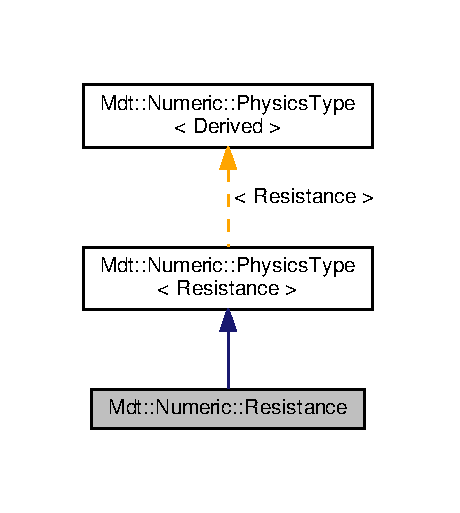
\includegraphics[width=221pt]{class_mdt_1_1_numeric_1_1_resistance__inherit__graph}
\end{center}
\end{figure}


Collaboration diagram for Mdt\+:\+:Numeric\+:\+:Resistance\+:\nopagebreak
\begin{figure}[H]
\begin{center}
\leavevmode
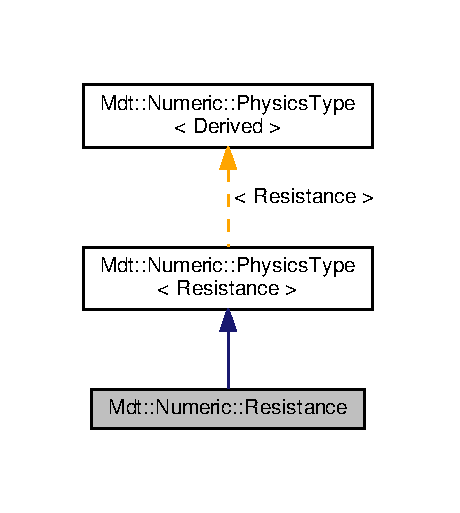
\includegraphics[width=221pt]{class_mdt_1_1_numeric_1_1_resistance__coll__graph}
\end{center}
\end{figure}
\subsection*{Public Member Functions}
\begin{DoxyCompactItemize}
\item 
constexpr \hyperlink{class_mdt_1_1_numeric_1_1_resistance_ad1f9115eeae7bb01b54e79d036b2c6f9}{Resistance} () noexcept\hypertarget{class_mdt_1_1_numeric_1_1_resistance_ad1f9115eeae7bb01b54e79d036b2c6f9}{}\label{class_mdt_1_1_numeric_1_1_resistance_ad1f9115eeae7bb01b54e79d036b2c6f9}

\begin{DoxyCompactList}\small\item\em Construct a null resistance. \end{DoxyCompactList}\item 
constexpr \hyperlink{class_mdt_1_1_numeric_1_1_resistance_aab313a78dbace4ea659e49c4353b53dc}{Resistance} (\hyperlink{class_mdt_1_1_numeric_1_1_double}{Double} r) noexcept\hypertarget{class_mdt_1_1_numeric_1_1_resistance_aab313a78dbace4ea659e49c4353b53dc}{}\label{class_mdt_1_1_numeric_1_1_resistance_aab313a78dbace4ea659e49c4353b53dc}

\begin{DoxyCompactList}\small\item\em Construct a resistance. \end{DoxyCompactList}\item 
constexpr \hyperlink{class_mdt_1_1_numeric_1_1_resistance_aec246aaa432d9d2985fa4bbfcb81abfb}{Resistance} (double r) noexcept\hypertarget{class_mdt_1_1_numeric_1_1_resistance_aec246aaa432d9d2985fa4bbfcb81abfb}{}\label{class_mdt_1_1_numeric_1_1_resistance_aec246aaa432d9d2985fa4bbfcb81abfb}

\begin{DoxyCompactList}\small\item\em Construct a resistance. \end{DoxyCompactList}\end{DoxyCompactItemize}
\subsection*{Static Public Member Functions}
\begin{DoxyCompactItemize}
\item 
static \hyperlink{class_mdt_1_1_numeric_1_1_resistance}{Resistance} \hyperlink{class_mdt_1_1_numeric_1_1_resistance_af2f9019a15179e5e7c13cd31b431c740}{from\+Q\+Variant} (const Q\+Variant \&r)
\begin{DoxyCompactList}\small\item\em Get resistance from a Q\+Variant. \end{DoxyCompactList}\end{DoxyCompactItemize}


\subsection{Detailed Description}
Value type that represents a resistance. 

Definition at line 31 of file Resistance.\+h.



\subsection{Member Function Documentation}
\index{Mdt\+::\+Numeric\+::\+Resistance@{Mdt\+::\+Numeric\+::\+Resistance}!from\+Q\+Variant@{from\+Q\+Variant}}
\index{from\+Q\+Variant@{from\+Q\+Variant}!Mdt\+::\+Numeric\+::\+Resistance@{Mdt\+::\+Numeric\+::\+Resistance}}
\subsubsection[{\texorpdfstring{from\+Q\+Variant(const Q\+Variant \&r)}{fromQVariant(const QVariant &r)}}]{\setlength{\rightskip}{0pt plus 5cm}static {\bf Resistance} Mdt\+::\+Numeric\+::\+Resistance\+::from\+Q\+Variant (
\begin{DoxyParamCaption}
\item[{const Q\+Variant \&}]{r}
\end{DoxyParamCaption}
)\hspace{0.3cm}{\ttfamily [inline]}, {\ttfamily [static]}}\hypertarget{class_mdt_1_1_numeric_1_1_resistance_af2f9019a15179e5e7c13cd31b431c740}{}\label{class_mdt_1_1_numeric_1_1_resistance_af2f9019a15179e5e7c13cd31b431c740}


Get resistance from a Q\+Variant. 

If r is null, a null resistance is returned

\begin{DoxyPrecond}{Precondition}
If r has a value (is not null), it must be convertible to double 
\end{DoxyPrecond}


Definition at line 56 of file Resistance.\+h.



The documentation for this class was generated from the following file\+:\begin{DoxyCompactItemize}
\item 
libs/\+Numeric/src/\+Mdt/\+Numeric/Resistance.\+h\end{DoxyCompactItemize}

\hypertarget{class_mdt_1_1_deploy_utils_1_1_search_path_list}{}\section{Mdt\+:\+:Deploy\+Utils\+:\+:Search\+Path\+List Class Reference}
\label{class_mdt_1_1_deploy_utils_1_1_search_path_list}\index{Mdt\+::\+Deploy\+Utils\+::\+Search\+Path\+List@{Mdt\+::\+Deploy\+Utils\+::\+Search\+Path\+List}}


\hyperlink{class_mdt_1_1_deploy_utils_1_1_search_path_list}{Search\+Path\+List} provides additional tools to \hyperlink{class_mdt_1_1_deploy_utils_1_1_path_list}{Path\+List}.  




{\ttfamily \#include $<$Search\+Path\+List.\+h$>$}

\subsection*{Public Member Functions}
\begin{DoxyCompactItemize}
\item 
void \hyperlink{class_mdt_1_1_deploy_utils_1_1_search_path_list_a3f10eadc3981b72ac9d2efc54484fa9a}{set\+Include\+Path\+Prefixes} (bool include)
\begin{DoxyCompactList}\small\item\em Specify if path prefixes must be part of the search paths. \end{DoxyCompactList}\item 
void \hyperlink{class_mdt_1_1_deploy_utils_1_1_search_path_list_ab850ca5b09572c85f38d9a2b0d56608b}{set\+Path\+Prefix\+List} (const \hyperlink{class_mdt_1_1_deploy_utils_1_1_path_list}{Path\+List} \&\hyperlink{class_mdt_1_1_deploy_utils_1_1_search_path_list_aa7c7f8f31e4ce1aaabdcdd03eb8f1256}{path\+List})
\begin{DoxyCompactList}\small\item\em Set a list of path prefix. \end{DoxyCompactList}\item 
void \hyperlink{class_mdt_1_1_deploy_utils_1_1_search_path_list_a80e2b88c150cf3916871845d041566f1}{set\+Path\+Suffix\+List} (const Q\+String\+List \&suffix\+List)
\begin{DoxyCompactList}\small\item\em Specify subdirectories to check. \end{DoxyCompactList}\item 
void \hyperlink{class_mdt_1_1_deploy_utils_1_1_search_path_list_ad06c34f840769dc0ba75fd3c3442ecbf}{append\+Path} (const Q\+String \&path)
\begin{DoxyCompactList}\small\item\em Append a path. \end{DoxyCompactList}\item 
void \hyperlink{class_mdt_1_1_deploy_utils_1_1_search_path_list_a09e1456243ac5616681d201f4fbbe1c1}{prepend\+Path} (const Q\+String \&path)
\begin{DoxyCompactList}\small\item\em Prepend a path. \end{DoxyCompactList}\item 
\hyperlink{class_mdt_1_1_deploy_utils_1_1_path_list}{Path\+List} \hyperlink{class_mdt_1_1_deploy_utils_1_1_search_path_list_aa7c7f8f31e4ce1aaabdcdd03eb8f1256}{path\+List} () const \hypertarget{class_mdt_1_1_deploy_utils_1_1_search_path_list_aa7c7f8f31e4ce1aaabdcdd03eb8f1256}{}\label{class_mdt_1_1_deploy_utils_1_1_search_path_list_aa7c7f8f31e4ce1aaabdcdd03eb8f1256}

\begin{DoxyCompactList}\small\item\em Get a list with all paths. \end{DoxyCompactList}\item 
Q\+String\+List \hyperlink{class_mdt_1_1_deploy_utils_1_1_search_path_list_a05ef6cbb6b33f72f5ea0f947295a4176}{to\+String\+List} () const \hypertarget{class_mdt_1_1_deploy_utils_1_1_search_path_list_a05ef6cbb6b33f72f5ea0f947295a4176}{}\label{class_mdt_1_1_deploy_utils_1_1_search_path_list_a05ef6cbb6b33f72f5ea0f947295a4176}

\begin{DoxyCompactList}\small\item\em Get a string list with all paths. \end{DoxyCompactList}\item 
void \hyperlink{class_mdt_1_1_deploy_utils_1_1_search_path_list_aced7be7dc12b60210a6b9f379585d693}{clear} ()\hypertarget{class_mdt_1_1_deploy_utils_1_1_search_path_list_aced7be7dc12b60210a6b9f379585d693}{}\label{class_mdt_1_1_deploy_utils_1_1_search_path_list_aced7be7dc12b60210a6b9f379585d693}

\begin{DoxyCompactList}\small\item\em Clear this list. \end{DoxyCompactList}\end{DoxyCompactItemize}


\subsection{Detailed Description}
\hyperlink{class_mdt_1_1_deploy_utils_1_1_search_path_list}{Search\+Path\+List} provides additional tools to \hyperlink{class_mdt_1_1_deploy_utils_1_1_path_list}{Path\+List}. 

Definition at line 32 of file Search\+Path\+List.\+h.



\subsection{Member Function Documentation}
\index{Mdt\+::\+Deploy\+Utils\+::\+Search\+Path\+List@{Mdt\+::\+Deploy\+Utils\+::\+Search\+Path\+List}!append\+Path@{append\+Path}}
\index{append\+Path@{append\+Path}!Mdt\+::\+Deploy\+Utils\+::\+Search\+Path\+List@{Mdt\+::\+Deploy\+Utils\+::\+Search\+Path\+List}}
\subsubsection[{\texorpdfstring{append\+Path(const Q\+String \&path)}{appendPath(const QString &path)}}]{\setlength{\rightskip}{0pt plus 5cm}void Mdt\+::\+Deploy\+Utils\+::\+Search\+Path\+List\+::append\+Path (
\begin{DoxyParamCaption}
\item[{const Q\+String \&}]{path}
\end{DoxyParamCaption}
)}\hypertarget{class_mdt_1_1_deploy_utils_1_1_search_path_list_ad06c34f840769dc0ba75fd3c3442ecbf}{}\label{class_mdt_1_1_deploy_utils_1_1_search_path_list_ad06c34f840769dc0ba75fd3c3442ecbf}


Append a path. 

Add {\itshape path} to the end of this list. Later, {\itshape path} will be returned as is, without any suffix. 

Definition at line 53 of file Search\+Path\+List.\+cpp.

\index{Mdt\+::\+Deploy\+Utils\+::\+Search\+Path\+List@{Mdt\+::\+Deploy\+Utils\+::\+Search\+Path\+List}!prepend\+Path@{prepend\+Path}}
\index{prepend\+Path@{prepend\+Path}!Mdt\+::\+Deploy\+Utils\+::\+Search\+Path\+List@{Mdt\+::\+Deploy\+Utils\+::\+Search\+Path\+List}}
\subsubsection[{\texorpdfstring{prepend\+Path(const Q\+String \&path)}{prependPath(const QString &path)}}]{\setlength{\rightskip}{0pt plus 5cm}void Mdt\+::\+Deploy\+Utils\+::\+Search\+Path\+List\+::prepend\+Path (
\begin{DoxyParamCaption}
\item[{const Q\+String \&}]{path}
\end{DoxyParamCaption}
)}\hypertarget{class_mdt_1_1_deploy_utils_1_1_search_path_list_a09e1456243ac5616681d201f4fbbe1c1}{}\label{class_mdt_1_1_deploy_utils_1_1_search_path_list_a09e1456243ac5616681d201f4fbbe1c1}


Prepend a path. 

Add {\itshape path} to the beginnig of this list. Later, {\itshape path} will be returned as is, without any suffix. 

Definition at line 47 of file Search\+Path\+List.\+cpp.

\index{Mdt\+::\+Deploy\+Utils\+::\+Search\+Path\+List@{Mdt\+::\+Deploy\+Utils\+::\+Search\+Path\+List}!set\+Include\+Path\+Prefixes@{set\+Include\+Path\+Prefixes}}
\index{set\+Include\+Path\+Prefixes@{set\+Include\+Path\+Prefixes}!Mdt\+::\+Deploy\+Utils\+::\+Search\+Path\+List@{Mdt\+::\+Deploy\+Utils\+::\+Search\+Path\+List}}
\subsubsection[{\texorpdfstring{set\+Include\+Path\+Prefixes(bool include)}{setIncludePathPrefixes(bool include)}}]{\setlength{\rightskip}{0pt plus 5cm}void Mdt\+::\+Deploy\+Utils\+::\+Search\+Path\+List\+::set\+Include\+Path\+Prefixes (
\begin{DoxyParamCaption}
\item[{bool}]{include}
\end{DoxyParamCaption}
)}\hypertarget{class_mdt_1_1_deploy_utils_1_1_search_path_list_a3f10eadc3981b72ac9d2efc54484fa9a}{}\label{class_mdt_1_1_deploy_utils_1_1_search_path_list_a3f10eadc3981b72ac9d2efc54484fa9a}


Specify if path prefixes must be part of the search paths. 

By default, path prefixes are not part of the search path. 

Definition at line 29 of file Search\+Path\+List.\+cpp.

\index{Mdt\+::\+Deploy\+Utils\+::\+Search\+Path\+List@{Mdt\+::\+Deploy\+Utils\+::\+Search\+Path\+List}!set\+Path\+Prefix\+List@{set\+Path\+Prefix\+List}}
\index{set\+Path\+Prefix\+List@{set\+Path\+Prefix\+List}!Mdt\+::\+Deploy\+Utils\+::\+Search\+Path\+List@{Mdt\+::\+Deploy\+Utils\+::\+Search\+Path\+List}}
\subsubsection[{\texorpdfstring{set\+Path\+Prefix\+List(const Path\+List \&path\+List)}{setPathPrefixList(const PathList &pathList)}}]{\setlength{\rightskip}{0pt plus 5cm}void Mdt\+::\+Deploy\+Utils\+::\+Search\+Path\+List\+::set\+Path\+Prefix\+List (
\begin{DoxyParamCaption}
\item[{const {\bf Path\+List} \&}]{path\+List}
\end{DoxyParamCaption}
)}\hypertarget{class_mdt_1_1_deploy_utils_1_1_search_path_list_ab850ca5b09572c85f38d9a2b0d56608b}{}\label{class_mdt_1_1_deploy_utils_1_1_search_path_list_ab850ca5b09572c85f38d9a2b0d56608b}


Set a list of path prefix. 

A path prefix is typically the root of a library distribution, which then contains subdirectories like bin, lib, ... 

Definition at line 35 of file Search\+Path\+List.\+cpp.

\index{Mdt\+::\+Deploy\+Utils\+::\+Search\+Path\+List@{Mdt\+::\+Deploy\+Utils\+::\+Search\+Path\+List}!set\+Path\+Suffix\+List@{set\+Path\+Suffix\+List}}
\index{set\+Path\+Suffix\+List@{set\+Path\+Suffix\+List}!Mdt\+::\+Deploy\+Utils\+::\+Search\+Path\+List@{Mdt\+::\+Deploy\+Utils\+::\+Search\+Path\+List}}
\subsubsection[{\texorpdfstring{set\+Path\+Suffix\+List(const Q\+String\+List \&suffix\+List)}{setPathSuffixList(const QStringList &suffixList)}}]{\setlength{\rightskip}{0pt plus 5cm}void Mdt\+::\+Deploy\+Utils\+::\+Search\+Path\+List\+::set\+Path\+Suffix\+List (
\begin{DoxyParamCaption}
\item[{const Q\+String\+List \&}]{suffix\+List}
\end{DoxyParamCaption}
)}\hypertarget{class_mdt_1_1_deploy_utils_1_1_search_path_list_a80e2b88c150cf3916871845d041566f1}{}\label{class_mdt_1_1_deploy_utils_1_1_search_path_list_a80e2b88c150cf3916871845d041566f1}


Specify subdirectories to check. 

Specify subdirectories to check below each directory in those specified with \hyperlink{class_mdt_1_1_deploy_utils_1_1_search_path_list_ab850ca5b09572c85f38d9a2b0d56608b}{set\+Path\+Prefix\+List()}. For example, if /opt/liba and /opt/libb have been set as path prefixes, and {\itshape suffix\+List} contains bin qt5/bin, path list will contain /opt/liba/bin, /opt/liba/qt5/bin, /opt/libb/bin, /opt/libb/qt5/bin . If include\+Path\+Prefixes is set, path list will contain /opt/liba, /opt/liba/bin, /opt/liba/qt5/bin, /opt/libb, /opt/libb/bin, /opt/libb/qt5/bin .

\begin{DoxySeeAlso}{See also}
\hyperlink{class_mdt_1_1_deploy_utils_1_1_search_path_list_ab850ca5b09572c85f38d9a2b0d56608b}{set\+Path\+Prefix\+List()} 

\hyperlink{class_mdt_1_1_deploy_utils_1_1_search_path_list_a3f10eadc3981b72ac9d2efc54484fa9a}{set\+Include\+Path\+Prefixes()} 
\end{DoxySeeAlso}


Definition at line 41 of file Search\+Path\+List.\+cpp.



The documentation for this class was generated from the following files\+:\begin{DoxyCompactItemize}
\item 
libs/\+Deploy\+Utils\+\_\+\+Core/src/\+Mdt/\+Deploy\+Utils/Search\+Path\+List.\+h\item 
libs/\+Deploy\+Utils\+\_\+\+Core/src/\+Mdt/\+Deploy\+Utils/Search\+Path\+List.\+cpp\end{DoxyCompactItemize}

\hypertarget{class_mdt_1_1_single_application}{}\section{Mdt\+:\+:Single\+Application Class Reference}
\label{class_mdt_1_1_single_application}\index{Mdt\+::\+Single\+Application@{Mdt\+::\+Single\+Application}}


\hyperlink{class_mdt_1_1_single_application}{Single\+Application} adds some helper to \hyperlink{class_qt_single_core_application}{Qt\+Single\+Core\+Application} for application initialization.  




{\ttfamily \#include $<$Single\+Application.\+h$>$}



Inheritance diagram for Mdt\+:\+:Single\+Application\+:\nopagebreak
\begin{figure}[H]
\begin{center}
\leavevmode
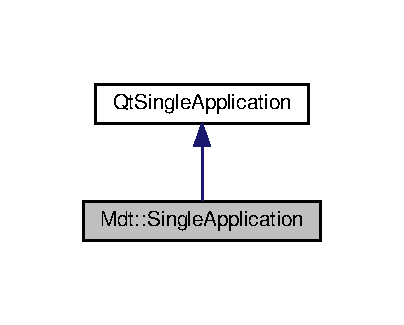
\includegraphics[width=194pt]{class_mdt_1_1_single_application__inherit__graph}
\end{center}
\end{figure}


Collaboration diagram for Mdt\+:\+:Single\+Application\+:\nopagebreak
\begin{figure}[H]
\begin{center}
\leavevmode
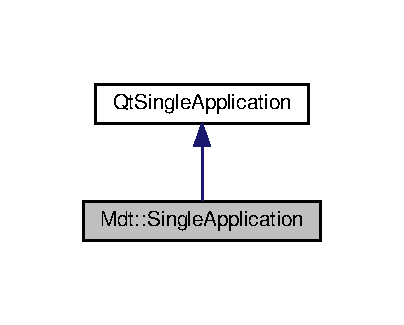
\includegraphics[width=194pt]{class_mdt_1_1_single_application__coll__graph}
\end{center}
\end{figure}
\subsection*{Public Member Functions}
\begin{DoxyCompactItemize}
\item 
\hyperlink{class_mdt_1_1_single_application_a481cd7bad65a75dd891ca33cb80c82c5}{Single\+Application} (int \&argc, char $\ast$$\ast$argv)\hypertarget{class_mdt_1_1_single_application_a481cd7bad65a75dd891ca33cb80c82c5}{}\label{class_mdt_1_1_single_application_a481cd7bad65a75dd891ca33cb80c82c5}

\begin{DoxyCompactList}\small\item\em Construct a single core application. \end{DoxyCompactList}\item 
\hyperlink{class_mdt_1_1_single_application_a49ff3421ee835333c6ebc00e8cdbf7ba}{$\sim$\+Single\+Application} ()\hypertarget{class_mdt_1_1_single_application_a49ff3421ee835333c6ebc00e8cdbf7ba}{}\label{class_mdt_1_1_single_application_a49ff3421ee835333c6ebc00e8cdbf7ba}

\begin{DoxyCompactList}\small\item\em Destroy the single core application object. \end{DoxyCompactList}\item 
void \hyperlink{class_mdt_1_1_single_application_abfd6a19af0b13b2785f2db7dd8db82a0}{enable\+File\+Logging} ()
\begin{DoxyCompactList}\small\item\em Enable file logging. \end{DoxyCompactList}\item 
Q\+String \hyperlink{class_mdt_1_1_single_application_a77ad0fd06b6b46107dc2f6c170325987}{log\+File\+Path} ()\hypertarget{class_mdt_1_1_single_application_a77ad0fd06b6b46107dc2f6c170325987}{}\label{class_mdt_1_1_single_application_a77ad0fd06b6b46107dc2f6c170325987}

\begin{DoxyCompactList}\small\item\em Get the path to the log file. \end{DoxyCompactList}\item 
void \hyperlink{class_mdt_1_1_single_application_a884f933e6b26b1a36b564e2b5e8f8536}{debug\+Environment} ()
\begin{DoxyCompactList}\small\item\em Debug environment. \end{DoxyCompactList}\end{DoxyCompactItemize}
\subsection*{Static Public Member Functions}
\begin{DoxyCompactItemize}
\item 
static Q\+String \hyperlink{class_mdt_1_1_single_application_a4f3aae54824f81697a17e7b1e173feec}{cache\+Directory\+Path} ()
\begin{DoxyCompactList}\small\item\em Get path to the cache directory. \end{DoxyCompactList}\item 
static Q\+String \hyperlink{class_mdt_1_1_single_application_a0f66bbb8cadc93f8185d3d4c92e3685e}{qt\+Version} ()\hypertarget{class_mdt_1_1_single_application_a0f66bbb8cadc93f8185d3d4c92e3685e}{}\label{class_mdt_1_1_single_application_a0f66bbb8cadc93f8185d3d4c92e3685e}

\begin{DoxyCompactList}\small\item\em Get Qt library version. \end{DoxyCompactList}\item 
static Q\+String \hyperlink{class_mdt_1_1_single_application_a9b31e7b78f87a9aa37ffadaf893b0cec}{mdt\+Version} ()\hypertarget{class_mdt_1_1_single_application_a9b31e7b78f87a9aa37ffadaf893b0cec}{}\label{class_mdt_1_1_single_application_a9b31e7b78f87a9aa37ffadaf893b0cec}

\begin{DoxyCompactList}\small\item\em Get \hyperlink{namespace_mdt}{Mdt} library version. \end{DoxyCompactList}\end{DoxyCompactItemize}
\subsection*{Additional Inherited Members}


\subsection{Detailed Description}
\hyperlink{class_mdt_1_1_single_application}{Single\+Application} adds some helper to \hyperlink{class_qt_single_core_application}{Qt\+Single\+Core\+Application} for application initialization. 

\begin{DoxySeeAlso}{See also}
\hyperlink{class_qt_single_core_application}{Qt\+Single\+Core\+Application} 

Q\+Core\+Application 
\end{DoxySeeAlso}


Definition at line 39 of file Single\+Application.\+h.



\subsection{Member Function Documentation}
\index{Mdt\+::\+Single\+Application@{Mdt\+::\+Single\+Application}!cache\+Directory\+Path@{cache\+Directory\+Path}}
\index{cache\+Directory\+Path@{cache\+Directory\+Path}!Mdt\+::\+Single\+Application@{Mdt\+::\+Single\+Application}}
\subsubsection[{\texorpdfstring{cache\+Directory\+Path()}{cacheDirectoryPath()}}]{\setlength{\rightskip}{0pt plus 5cm}Q\+String Mdt\+::\+Single\+Application\+::cache\+Directory\+Path (
\begin{DoxyParamCaption}
{}
\end{DoxyParamCaption}
)\hspace{0.3cm}{\ttfamily [static]}}\hypertarget{class_mdt_1_1_single_application_a4f3aae54824f81697a17e7b1e173feec}{}\label{class_mdt_1_1_single_application_a4f3aae54824f81697a17e7b1e173feec}


Get path to the cache directory. 

Returns \hyperlink{class_mdt_1_1_standard_paths_a2ca803e5a6b9fb2a4808968becfb86de}{Standard\+Paths\+::cache\+Directory\+Path()} 

Definition at line 45 of file Single\+Application.\+cpp.

\index{Mdt\+::\+Single\+Application@{Mdt\+::\+Single\+Application}!debug\+Environment@{debug\+Environment}}
\index{debug\+Environment@{debug\+Environment}!Mdt\+::\+Single\+Application@{Mdt\+::\+Single\+Application}}
\subsubsection[{\texorpdfstring{debug\+Environment()}{debugEnvironment()}}]{\setlength{\rightskip}{0pt plus 5cm}void Mdt\+::\+Single\+Application\+::debug\+Environment (
\begin{DoxyParamCaption}
{}
\end{DoxyParamCaption}
)}\hypertarget{class_mdt_1_1_single_application_a884f933e6b26b1a36b564e2b5e8f8536}{}\label{class_mdt_1_1_single_application_a884f933e6b26b1a36b564e2b5e8f8536}


Debug environment. 

Will print various informations, like libraries versions, paths to some directories, etc.. to the console. 

Definition at line 60 of file Single\+Application.\+cpp.

\index{Mdt\+::\+Single\+Application@{Mdt\+::\+Single\+Application}!enable\+File\+Logging@{enable\+File\+Logging}}
\index{enable\+File\+Logging@{enable\+File\+Logging}!Mdt\+::\+Single\+Application@{Mdt\+::\+Single\+Application}}
\subsubsection[{\texorpdfstring{enable\+File\+Logging()}{enableFileLogging()}}]{\setlength{\rightskip}{0pt plus 5cm}void Mdt\+::\+Single\+Application\+::enable\+File\+Logging (
\begin{DoxyParamCaption}
{}
\end{DoxyParamCaption}
)}\hypertarget{class_mdt_1_1_single_application_abfd6a19af0b13b2785f2db7dd8db82a0}{}\label{class_mdt_1_1_single_application_abfd6a19af0b13b2785f2db7dd8db82a0}


Enable file logging. 

After file logging was enabled, errors that are committed using \hyperlink{class_mdt_1_1_error_a1b4a57bd4177d2985abd62b6b49a43f8}{Mdt\+::\+Error\+::commit()} are added to the log file {\itshape \hyperlink{class_mdt_1_1_single_application_a77ad0fd06b6b46107dc2f6c170325987}{log\+File\+Path()}} . 

Definition at line 35 of file Single\+Application.\+cpp.



The documentation for this class was generated from the following files\+:\begin{DoxyCompactItemize}
\item 
libs/\+Application\+\_\+\+Widgets\+\_\+\+Single/src/\+Mdt/Single\+Application.\+h\item 
libs/\+Application\+\_\+\+Widgets\+\_\+\+Single/src/\+Mdt/Single\+Application.\+cpp\end{DoxyCompactItemize}

\hypertarget{class_mdt_1_1_single_core_application}{}\section{Mdt\+:\+:Single\+Core\+Application Class Reference}
\label{class_mdt_1_1_single_core_application}\index{Mdt\+::\+Single\+Core\+Application@{Mdt\+::\+Single\+Core\+Application}}


\hyperlink{class_mdt_1_1_single_core_application}{Single\+Core\+Application} adds some helper to \hyperlink{class_qt_single_core_application}{Qt\+Single\+Core\+Application} for application initialization.  




{\ttfamily \#include $<$Single\+Core\+Application.\+h$>$}



Inheritance diagram for Mdt\+:\+:Single\+Core\+Application\+:
\nopagebreak
\begin{figure}[H]
\begin{center}
\leavevmode
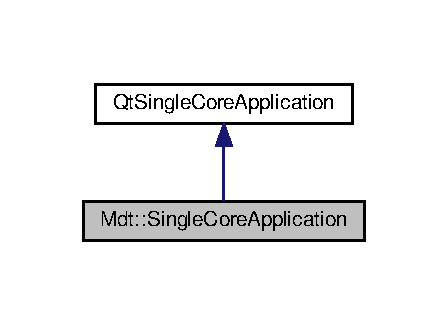
\includegraphics[width=215pt]{class_mdt_1_1_single_core_application__inherit__graph}
\end{center}
\end{figure}


Collaboration diagram for Mdt\+:\+:Single\+Core\+Application\+:
\nopagebreak
\begin{figure}[H]
\begin{center}
\leavevmode
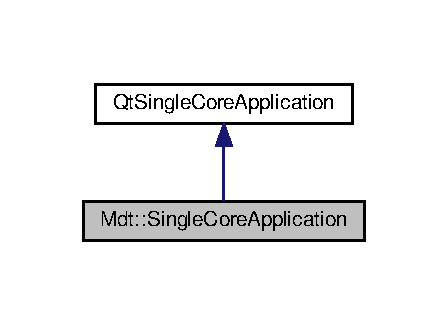
\includegraphics[width=215pt]{class_mdt_1_1_single_core_application__coll__graph}
\end{center}
\end{figure}
\subsection*{Public Member Functions}
\begin{DoxyCompactItemize}
\item 
\hyperlink{class_mdt_1_1_single_core_application_a18493beac6e321df7852571ed4a55205}{Single\+Core\+Application} (int \&argc, char $\ast$$\ast$argv)
\begin{DoxyCompactList}\small\item\em Construct a single core application. \end{DoxyCompactList}\item 
\hyperlink{class_mdt_1_1_single_core_application_ab3a61d6e1a5b36be02de6eba1c2f3867}{$\sim$\+Single\+Core\+Application} ()
\begin{DoxyCompactList}\small\item\em Destroy the single core application object. \end{DoxyCompactList}\item 
{\bfseries Single\+Core\+Application} (const \hyperlink{class_mdt_1_1_single_core_application}{Single\+Core\+Application} \&)=delete\hypertarget{class_mdt_1_1_single_core_application_a3e0683245258cb0aacf53af2976e54b1}{}\label{class_mdt_1_1_single_core_application_a3e0683245258cb0aacf53af2976e54b1}

\item 
\hyperlink{class_mdt_1_1_single_core_application}{Single\+Core\+Application} \& {\bfseries operator=} (const \hyperlink{class_mdt_1_1_single_core_application}{Single\+Core\+Application} \&)=delete\hypertarget{class_mdt_1_1_single_core_application_a1b20009662a270d9522c26b1e5d160fa}{}\label{class_mdt_1_1_single_core_application_a1b20009662a270d9522c26b1e5d160fa}

\item 
{\bfseries Single\+Core\+Application} (\hyperlink{class_mdt_1_1_single_core_application}{Single\+Core\+Application} \&\&)=delete\hypertarget{class_mdt_1_1_single_core_application_ae95bdbe03d440d8a344bdfe7b9f5802e}{}\label{class_mdt_1_1_single_core_application_ae95bdbe03d440d8a344bdfe7b9f5802e}

\item 
\hyperlink{class_mdt_1_1_single_core_application}{Single\+Core\+Application} \& {\bfseries operator=} (\hyperlink{class_mdt_1_1_single_core_application}{Single\+Core\+Application} \&\&)=delete\hypertarget{class_mdt_1_1_single_core_application_a268b15bee0658b536afa3c7bdf0ea48e}{}\label{class_mdt_1_1_single_core_application_a268b15bee0658b536afa3c7bdf0ea48e}

\item 
void \hyperlink{class_mdt_1_1_single_core_application_ae9084643bbbc67ce795dca5d6aae35fe}{enable\+File\+Logging} ()
\begin{DoxyCompactList}\small\item\em Enable file logging. \end{DoxyCompactList}\item 
Q\+String \hyperlink{class_mdt_1_1_single_core_application_a3f680ab0c6467712d7ba495e20adbafa}{log\+File\+Path} ()
\begin{DoxyCompactList}\small\item\em Get the path to the log file. \end{DoxyCompactList}\item 
void \hyperlink{class_mdt_1_1_single_core_application_a95e8cfb94a48a1c52e5896b74c78783f}{debug\+Environment} ()
\begin{DoxyCompactList}\small\item\em Debug environment. \end{DoxyCompactList}\end{DoxyCompactItemize}
\subsection*{Static Public Member Functions}
\begin{DoxyCompactItemize}
\item 
static Q\+String \hyperlink{class_mdt_1_1_single_core_application_a9081eaa0ddfc35ed1360f64fbe52c18a}{cache\+Directory\+Path} ()
\begin{DoxyCompactList}\small\item\em Get path to the cache directory. \end{DoxyCompactList}\item 
static Q\+String \hyperlink{class_mdt_1_1_single_core_application_a19c7ede35e9fe6beca09d49235327a34}{qt\+Version} ()
\begin{DoxyCompactList}\small\item\em Get Qt library version. \end{DoxyCompactList}\item 
static Q\+String \hyperlink{class_mdt_1_1_single_core_application_a17db75d06f3ba6be926f39620c45b383}{mdt\+Version} ()
\begin{DoxyCompactList}\small\item\em Get \hyperlink{namespace_mdt}{Mdt} library version. \end{DoxyCompactList}\end{DoxyCompactItemize}
\subsection*{Additional Inherited Members}


\subsection{Detailed Description}
\hyperlink{class_mdt_1_1_single_core_application}{Single\+Core\+Application} adds some helper to \hyperlink{class_qt_single_core_application}{Qt\+Single\+Core\+Application} for application initialization. 

\begin{DoxySeeAlso}{See also}
\hyperlink{class_qt_single_core_application}{Qt\+Single\+Core\+Application} 

\hyperlink{class_q_core_application}{Q\+Core\+Application} 
\end{DoxySeeAlso}


Definition at line 38 of file Single\+Core\+Application.\+h.



\subsection{Constructor \& Destructor Documentation}
\index{Mdt\+::\+Single\+Core\+Application@{Mdt\+::\+Single\+Core\+Application}!Single\+Core\+Application@{Single\+Core\+Application}}
\index{Single\+Core\+Application@{Single\+Core\+Application}!Mdt\+::\+Single\+Core\+Application@{Mdt\+::\+Single\+Core\+Application}}
\subsubsection[{\texorpdfstring{Single\+Core\+Application(int \&argc, char $\ast$$\ast$argv)}{SingleCoreApplication(int &argc, char **argv)}}]{\setlength{\rightskip}{0pt plus 5cm}Mdt\+::\+Single\+Core\+Application\+::\+Single\+Core\+Application (
\begin{DoxyParamCaption}
\item[{int \&}]{argc, }
\item[{char $\ast$$\ast$}]{argv}
\end{DoxyParamCaption}
)}\hypertarget{class_mdt_1_1_single_core_application_a18493beac6e321df7852571ed4a55205}{}\label{class_mdt_1_1_single_core_application_a18493beac6e321df7852571ed4a55205}


Construct a single core application. 



Definition at line 25 of file Single\+Core\+Application.\+cpp.

\index{Mdt\+::\+Single\+Core\+Application@{Mdt\+::\+Single\+Core\+Application}!````~Single\+Core\+Application@{$\sim$\+Single\+Core\+Application}}
\index{````~Single\+Core\+Application@{$\sim$\+Single\+Core\+Application}!Mdt\+::\+Single\+Core\+Application@{Mdt\+::\+Single\+Core\+Application}}
\subsubsection[{\texorpdfstring{$\sim$\+Single\+Core\+Application()}{~SingleCoreApplication()}}]{\setlength{\rightskip}{0pt plus 5cm}Mdt\+::\+Single\+Core\+Application\+::$\sim$\+Single\+Core\+Application (
\begin{DoxyParamCaption}
{}
\end{DoxyParamCaption}
)}\hypertarget{class_mdt_1_1_single_core_application_ab3a61d6e1a5b36be02de6eba1c2f3867}{}\label{class_mdt_1_1_single_core_application_ab3a61d6e1a5b36be02de6eba1c2f3867}


Destroy the single core application object. 



Definition at line 31 of file Single\+Core\+Application.\+cpp.



\subsection{Member Function Documentation}
\index{Mdt\+::\+Single\+Core\+Application@{Mdt\+::\+Single\+Core\+Application}!cache\+Directory\+Path@{cache\+Directory\+Path}}
\index{cache\+Directory\+Path@{cache\+Directory\+Path}!Mdt\+::\+Single\+Core\+Application@{Mdt\+::\+Single\+Core\+Application}}
\subsubsection[{\texorpdfstring{cache\+Directory\+Path()}{cacheDirectoryPath()}}]{\setlength{\rightskip}{0pt plus 5cm}Q\+String Mdt\+::\+Single\+Core\+Application\+::cache\+Directory\+Path (
\begin{DoxyParamCaption}
{}
\end{DoxyParamCaption}
)\hspace{0.3cm}{\ttfamily [static]}}\hypertarget{class_mdt_1_1_single_core_application_a9081eaa0ddfc35ed1360f64fbe52c18a}{}\label{class_mdt_1_1_single_core_application_a9081eaa0ddfc35ed1360f64fbe52c18a}


Get path to the cache directory. 

Returns \hyperlink{class_mdt_1_1_standard_paths_a2ca803e5a6b9fb2a4808968becfb86de}{Standard\+Paths\+::cache\+Directory\+Path()} 

Definition at line 45 of file Single\+Core\+Application.\+cpp.

\index{Mdt\+::\+Single\+Core\+Application@{Mdt\+::\+Single\+Core\+Application}!debug\+Environment@{debug\+Environment}}
\index{debug\+Environment@{debug\+Environment}!Mdt\+::\+Single\+Core\+Application@{Mdt\+::\+Single\+Core\+Application}}
\subsubsection[{\texorpdfstring{debug\+Environment()}{debugEnvironment()}}]{\setlength{\rightskip}{0pt plus 5cm}void Mdt\+::\+Single\+Core\+Application\+::debug\+Environment (
\begin{DoxyParamCaption}
{}
\end{DoxyParamCaption}
)}\hypertarget{class_mdt_1_1_single_core_application_a95e8cfb94a48a1c52e5896b74c78783f}{}\label{class_mdt_1_1_single_core_application_a95e8cfb94a48a1c52e5896b74c78783f}


Debug environment. 

Will print various informations, like libraries versions, paths to some directories, etc.. to the console. 

Definition at line 60 of file Single\+Core\+Application.\+cpp.

\index{Mdt\+::\+Single\+Core\+Application@{Mdt\+::\+Single\+Core\+Application}!enable\+File\+Logging@{enable\+File\+Logging}}
\index{enable\+File\+Logging@{enable\+File\+Logging}!Mdt\+::\+Single\+Core\+Application@{Mdt\+::\+Single\+Core\+Application}}
\subsubsection[{\texorpdfstring{enable\+File\+Logging()}{enableFileLogging()}}]{\setlength{\rightskip}{0pt plus 5cm}void Mdt\+::\+Single\+Core\+Application\+::enable\+File\+Logging (
\begin{DoxyParamCaption}
{}
\end{DoxyParamCaption}
)}\hypertarget{class_mdt_1_1_single_core_application_ae9084643bbbc67ce795dca5d6aae35fe}{}\label{class_mdt_1_1_single_core_application_ae9084643bbbc67ce795dca5d6aae35fe}


Enable file logging. 

After file logging was enabled, errors that are committed using \hyperlink{class_mdt_1_1_error_a1b4a57bd4177d2985abd62b6b49a43f8}{Mdt\+::\+Error\+::commit()} are added to the log file {\itshape \hyperlink{class_mdt_1_1_single_core_application_a3f680ab0c6467712d7ba495e20adbafa}{log\+File\+Path()}} . 

Definition at line 35 of file Single\+Core\+Application.\+cpp.

\index{Mdt\+::\+Single\+Core\+Application@{Mdt\+::\+Single\+Core\+Application}!log\+File\+Path@{log\+File\+Path}}
\index{log\+File\+Path@{log\+File\+Path}!Mdt\+::\+Single\+Core\+Application@{Mdt\+::\+Single\+Core\+Application}}
\subsubsection[{\texorpdfstring{log\+File\+Path()}{logFilePath()}}]{\setlength{\rightskip}{0pt plus 5cm}Q\+String Mdt\+::\+Single\+Core\+Application\+::log\+File\+Path (
\begin{DoxyParamCaption}
{}
\end{DoxyParamCaption}
)}\hypertarget{class_mdt_1_1_single_core_application_a3f680ab0c6467712d7ba495e20adbafa}{}\label{class_mdt_1_1_single_core_application_a3f680ab0c6467712d7ba495e20adbafa}


Get the path to the log file. 



Definition at line 40 of file Single\+Core\+Application.\+cpp.

\index{Mdt\+::\+Single\+Core\+Application@{Mdt\+::\+Single\+Core\+Application}!mdt\+Version@{mdt\+Version}}
\index{mdt\+Version@{mdt\+Version}!Mdt\+::\+Single\+Core\+Application@{Mdt\+::\+Single\+Core\+Application}}
\subsubsection[{\texorpdfstring{mdt\+Version()}{mdtVersion()}}]{\setlength{\rightskip}{0pt plus 5cm}Q\+String Mdt\+::\+Single\+Core\+Application\+::mdt\+Version (
\begin{DoxyParamCaption}
{}
\end{DoxyParamCaption}
)\hspace{0.3cm}{\ttfamily [static]}}\hypertarget{class_mdt_1_1_single_core_application_a17db75d06f3ba6be926f39620c45b383}{}\label{class_mdt_1_1_single_core_application_a17db75d06f3ba6be926f39620c45b383}


Get \hyperlink{namespace_mdt}{Mdt} library version. 



Definition at line 55 of file Single\+Core\+Application.\+cpp.

\index{Mdt\+::\+Single\+Core\+Application@{Mdt\+::\+Single\+Core\+Application}!qt\+Version@{qt\+Version}}
\index{qt\+Version@{qt\+Version}!Mdt\+::\+Single\+Core\+Application@{Mdt\+::\+Single\+Core\+Application}}
\subsubsection[{\texorpdfstring{qt\+Version()}{qtVersion()}}]{\setlength{\rightskip}{0pt plus 5cm}Q\+String Mdt\+::\+Single\+Core\+Application\+::qt\+Version (
\begin{DoxyParamCaption}
{}
\end{DoxyParamCaption}
)\hspace{0.3cm}{\ttfamily [static]}}\hypertarget{class_mdt_1_1_single_core_application_a19c7ede35e9fe6beca09d49235327a34}{}\label{class_mdt_1_1_single_core_application_a19c7ede35e9fe6beca09d49235327a34}


Get Qt library version. 



Definition at line 50 of file Single\+Core\+Application.\+cpp.



The documentation for this class was generated from the following files\+:\begin{DoxyCompactItemize}
\item 
libs/\+Application\+\_\+\+Core\+\_\+\+Single/src/\+Mdt/Single\+Core\+Application.\+h\item 
libs/\+Application\+\_\+\+Core\+\_\+\+Single/src/\+Mdt/Single\+Core\+Application.\+cpp\end{DoxyCompactItemize}

\hypertarget{class_mdt_1_1_standard_paths}{}\section{Mdt\+:\+:Standard\+Paths Class Reference}
\label{class_mdt_1_1_standard_paths}\index{Mdt\+::\+Standard\+Paths@{Mdt\+::\+Standard\+Paths}}


Provides methods for accessing standard paths.  




{\ttfamily \#include $<$Standard\+Paths.\+h$>$}

\subsection*{Static Public Member Functions}
\begin{DoxyCompactItemize}
\item 
static Q\+String \hyperlink{class_mdt_1_1_standard_paths_aa45caeb4d2b4a5c539d301d800a7deac}{log\+Directory\+Path} ()
\begin{DoxyCompactList}\small\item\em Get path to the log file directory. \end{DoxyCompactList}\item 
static Q\+String \hyperlink{class_mdt_1_1_standard_paths_a2ca803e5a6b9fb2a4808968becfb86de}{cache\+Directory\+Path} ()
\begin{DoxyCompactList}\small\item\em Get path to the cache directory. \end{DoxyCompactList}\end{DoxyCompactItemize}


\subsection{Detailed Description}
Provides methods for accessing standard paths. 

This class uses Q\+Standard\+Paths and adds some additionnal paths defined for the \hyperlink{namespace_mdt}{Mdt} library. 

Definition at line 33 of file Standard\+Paths.\+h.



\subsection{Member Function Documentation}
\index{Mdt\+::\+Standard\+Paths@{Mdt\+::\+Standard\+Paths}!cache\+Directory\+Path@{cache\+Directory\+Path}}
\index{cache\+Directory\+Path@{cache\+Directory\+Path}!Mdt\+::\+Standard\+Paths@{Mdt\+::\+Standard\+Paths}}
\subsubsection[{\texorpdfstring{cache\+Directory\+Path()}{cacheDirectoryPath()}}]{\setlength{\rightskip}{0pt plus 5cm}Q\+String Mdt\+::\+Standard\+Paths\+::cache\+Directory\+Path (
\begin{DoxyParamCaption}
{}
\end{DoxyParamCaption}
)\hspace{0.3cm}{\ttfamily [static]}}\hypertarget{class_mdt_1_1_standard_paths_a2ca803e5a6b9fb2a4808968becfb86de}{}\label{class_mdt_1_1_standard_paths_a2ca803e5a6b9fb2a4808968becfb86de}


Get path to the cache directory. 

Returns a path to a writable location located in Q\+Standard\+Paths\+::\+Cache\+Location 

Definition at line 37 of file Standard\+Paths.\+cpp.



Referenced by Mdt\+::\+Core\+Application\+Impl\+::cache\+Directory\+Path().

\index{Mdt\+::\+Standard\+Paths@{Mdt\+::\+Standard\+Paths}!log\+Directory\+Path@{log\+Directory\+Path}}
\index{log\+Directory\+Path@{log\+Directory\+Path}!Mdt\+::\+Standard\+Paths@{Mdt\+::\+Standard\+Paths}}
\subsubsection[{\texorpdfstring{log\+Directory\+Path()}{logDirectoryPath()}}]{\setlength{\rightskip}{0pt plus 5cm}Q\+String Mdt\+::\+Standard\+Paths\+::log\+Directory\+Path (
\begin{DoxyParamCaption}
{}
\end{DoxyParamCaption}
)\hspace{0.3cm}{\ttfamily [static]}}\hypertarget{class_mdt_1_1_standard_paths_aa45caeb4d2b4a5c539d301d800a7deac}{}\label{class_mdt_1_1_standard_paths_aa45caeb4d2b4a5c539d301d800a7deac}


Get path to the log file directory. 

Returns a path to a writable location located in Q\+Standard\+Paths\+::\+App\+Data\+Location/log 

Definition at line 32 of file Standard\+Paths.\+cpp.



Referenced by Mdt\+::\+Core\+Application\+Impl\+::log\+Directory\+Path().



The documentation for this class was generated from the following files\+:\begin{DoxyCompactItemize}
\item 
libs/\+Application\+\_\+\+Core/src/\+Mdt/Standard\+Paths.\+h\item 
libs/\+Application\+\_\+\+Core/src/\+Mdt/Standard\+Paths.\+cpp\end{DoxyCompactItemize}

\hypertarget{struct_mdt_1_1_plain_text_1_1_string_const_iterator}{}\section{Mdt\+:\+:Plain\+Text\+:\+:String\+Const\+Iterator Struct Reference}
\label{struct_mdt_1_1_plain_text_1_1_string_const_iterator}\index{Mdt\+::\+Plain\+Text\+::\+String\+Const\+Iterator@{Mdt\+::\+Plain\+Text\+::\+String\+Const\+Iterator}}


Iterator that acts on Q\+String.  




{\ttfamily \#include $<$String\+Const\+Iterator.\+h$>$}

\subsection*{Public Member Functions}
\begin{DoxyCompactItemize}
\item 
\hyperlink{struct_mdt_1_1_plain_text_1_1_string_const_iterator_aebc75afef8accb5faf0dc33d065f898f}{String\+Const\+Iterator} ()
\begin{DoxyCompactList}\small\item\em Default constructor. \end{DoxyCompactList}\item 
\hyperlink{struct_mdt_1_1_plain_text_1_1_string_const_iterator_ae2cad12d2b7751eaf0a00a69678275ec}{String\+Const\+Iterator} (Q\+String\+::const\+\_\+iterator it)\hypertarget{struct_mdt_1_1_plain_text_1_1_string_const_iterator_ae2cad12d2b7751eaf0a00a69678275ec}{}\label{struct_mdt_1_1_plain_text_1_1_string_const_iterator_ae2cad12d2b7751eaf0a00a69678275ec}

\begin{DoxyCompactList}\small\item\em Constructor. \end{DoxyCompactList}\item 
\hyperlink{struct_mdt_1_1_plain_text_1_1_string_const_iterator}{String\+Const\+Iterator} \& \hyperlink{struct_mdt_1_1_plain_text_1_1_string_const_iterator_a5ff7bd8002a95fcb2e1aed0a27d4d60c}{operator=} (const \hyperlink{struct_mdt_1_1_plain_text_1_1_string_const_iterator}{String\+Const\+Iterator} \&other)\hypertarget{struct_mdt_1_1_plain_text_1_1_string_const_iterator_a5ff7bd8002a95fcb2e1aed0a27d4d60c}{}\label{struct_mdt_1_1_plain_text_1_1_string_const_iterator_a5ff7bd8002a95fcb2e1aed0a27d4d60c}

\begin{DoxyCompactList}\small\item\em Assignement. \end{DoxyCompactList}\item 
\hyperlink{struct_mdt_1_1_plain_text_1_1_string_const_iterator}{String\+Const\+Iterator} \& \hyperlink{struct_mdt_1_1_plain_text_1_1_string_const_iterator_acff7207d9b0257518a2845dbbce19f0f}{operator=} (Q\+String\+::const\+\_\+iterator \&it)\hypertarget{struct_mdt_1_1_plain_text_1_1_string_const_iterator_acff7207d9b0257518a2845dbbce19f0f}{}\label{struct_mdt_1_1_plain_text_1_1_string_const_iterator_acff7207d9b0257518a2845dbbce19f0f}

\begin{DoxyCompactList}\small\item\em Assignement. \end{DoxyCompactList}\item 
\hyperlink{struct_mdt_1_1_plain_text_1_1_string_const_iterator}{String\+Const\+Iterator} \& \hyperlink{struct_mdt_1_1_plain_text_1_1_string_const_iterator_a289ce7f324a31e2d0977ba6e9b5460dc}{operator++} ()\hypertarget{struct_mdt_1_1_plain_text_1_1_string_const_iterator_a289ce7f324a31e2d0977ba6e9b5460dc}{}\label{struct_mdt_1_1_plain_text_1_1_string_const_iterator_a289ce7f324a31e2d0977ba6e9b5460dc}

\begin{DoxyCompactList}\small\item\em Increment iterator (pre-\/increment) \end{DoxyCompactList}\item 
\hyperlink{struct_mdt_1_1_plain_text_1_1_string_const_iterator}{String\+Const\+Iterator} \hyperlink{struct_mdt_1_1_plain_text_1_1_string_const_iterator_a107f05451d845ef3371adc7300f52b03}{operator++} (int)\hypertarget{struct_mdt_1_1_plain_text_1_1_string_const_iterator_a107f05451d845ef3371adc7300f52b03}{}\label{struct_mdt_1_1_plain_text_1_1_string_const_iterator_a107f05451d845ef3371adc7300f52b03}

\begin{DoxyCompactList}\small\item\em Increment iterator (post-\/increment) \end{DoxyCompactList}\item 
\hyperlink{struct_mdt_1_1_plain_text_1_1_string_const_iterator}{String\+Const\+Iterator} \& \hyperlink{struct_mdt_1_1_plain_text_1_1_string_const_iterator_a1d923d5a9c0cb79d2b794587660ad376}{operator-\/-\/} ()\hypertarget{struct_mdt_1_1_plain_text_1_1_string_const_iterator_a1d923d5a9c0cb79d2b794587660ad376}{}\label{struct_mdt_1_1_plain_text_1_1_string_const_iterator_a1d923d5a9c0cb79d2b794587660ad376}

\begin{DoxyCompactList}\small\item\em Decrement iterator (pre-\/decrement) \end{DoxyCompactList}\item 
\hyperlink{struct_mdt_1_1_plain_text_1_1_string_const_iterator}{String\+Const\+Iterator} \hyperlink{struct_mdt_1_1_plain_text_1_1_string_const_iterator_ac80031fc5261a7aaf0c2229946483efb}{operator-\/-\/} (int)\hypertarget{struct_mdt_1_1_plain_text_1_1_string_const_iterator_ac80031fc5261a7aaf0c2229946483efb}{}\label{struct_mdt_1_1_plain_text_1_1_string_const_iterator_ac80031fc5261a7aaf0c2229946483efb}

\begin{DoxyCompactList}\small\item\em Decrement iterator (post-\/decrement) \end{DoxyCompactList}\item 
\hyperlink{struct_mdt_1_1_plain_text_1_1_string_const_iterator}{String\+Const\+Iterator} \hyperlink{struct_mdt_1_1_plain_text_1_1_string_const_iterator_ac7fd84c109231856126ecd9443792296}{operator-\/} (difference\+\_\+type n) const \hypertarget{struct_mdt_1_1_plain_text_1_1_string_const_iterator_ac7fd84c109231856126ecd9443792296}{}\label{struct_mdt_1_1_plain_text_1_1_string_const_iterator_ac7fd84c109231856126ecd9443792296}

\begin{DoxyCompactList}\small\item\em Returns a iterator that is rewind by n positions. \end{DoxyCompactList}\item 
\hyperlink{struct_mdt_1_1_plain_text_1_1_string_const_iterator}{String\+Const\+Iterator} \& \hyperlink{struct_mdt_1_1_plain_text_1_1_string_const_iterator_a2fdef53991d8a75174f6254ad4664c08}{operator+=} (difference\+\_\+type n)\hypertarget{struct_mdt_1_1_plain_text_1_1_string_const_iterator_a2fdef53991d8a75174f6254ad4664c08}{}\label{struct_mdt_1_1_plain_text_1_1_string_const_iterator_a2fdef53991d8a75174f6254ad4664c08}

\begin{DoxyCompactList}\small\item\em Advance iterator by n positions. \end{DoxyCompactList}\item 
\hyperlink{struct_mdt_1_1_plain_text_1_1_string_const_iterator}{String\+Const\+Iterator} \& \hyperlink{struct_mdt_1_1_plain_text_1_1_string_const_iterator_a20fc6889ac0e76812a993014f4d8e13b}{operator-\/=} (difference\+\_\+type n)\hypertarget{struct_mdt_1_1_plain_text_1_1_string_const_iterator_a20fc6889ac0e76812a993014f4d8e13b}{}\label{struct_mdt_1_1_plain_text_1_1_string_const_iterator_a20fc6889ac0e76812a993014f4d8e13b}

\begin{DoxyCompactList}\small\item\em Rewind iterator by n positions. \end{DoxyCompactList}\item 
value\+\_\+type \hyperlink{struct_mdt_1_1_plain_text_1_1_string_const_iterator_ad23073b28d2844ad3e3555608e4a9bd5}{operator$\ast$} () const \hypertarget{struct_mdt_1_1_plain_text_1_1_string_const_iterator_ad23073b28d2844ad3e3555608e4a9bd5}{}\label{struct_mdt_1_1_plain_text_1_1_string_const_iterator_ad23073b28d2844ad3e3555608e4a9bd5}

\begin{DoxyCompactList}\small\item\em Get pointed value. \end{DoxyCompactList}\item 
value\+\_\+type \hyperlink{struct_mdt_1_1_plain_text_1_1_string_const_iterator_a8a9673923bfd2e0af6f31b9f98ef8f46}{operator\mbox{[}$\,$\mbox{]}} (difference\+\_\+type i) const \hypertarget{struct_mdt_1_1_plain_text_1_1_string_const_iterator_a8a9673923bfd2e0af6f31b9f98ef8f46}{}\label{struct_mdt_1_1_plain_text_1_1_string_const_iterator_a8a9673923bfd2e0af6f31b9f98ef8f46}

\begin{DoxyCompactList}\small\item\em Get value by index. \end{DoxyCompactList}\end{DoxyCompactItemize}
\subsection*{Friends}
\begin{DoxyCompactItemize}
\item 
\hyperlink{struct_mdt_1_1_plain_text_1_1_string_const_iterator}{String\+Const\+Iterator} \hyperlink{struct_mdt_1_1_plain_text_1_1_string_const_iterator_aa6f9bb8b739cc2e480b3832e51f2311b}{operator+} (const \hyperlink{struct_mdt_1_1_plain_text_1_1_string_const_iterator}{String\+Const\+Iterator} \&a, difference\+\_\+type n)\hypertarget{struct_mdt_1_1_plain_text_1_1_string_const_iterator_aa6f9bb8b739cc2e480b3832e51f2311b}{}\label{struct_mdt_1_1_plain_text_1_1_string_const_iterator_aa6f9bb8b739cc2e480b3832e51f2311b}

\begin{DoxyCompactList}\small\item\em Returns a iterator resulting from {\itshape a} + {\itshape n}. \end{DoxyCompactList}\item 
\hyperlink{struct_mdt_1_1_plain_text_1_1_string_const_iterator}{String\+Const\+Iterator} \hyperlink{struct_mdt_1_1_plain_text_1_1_string_const_iterator_abeed2837c5315658a676d9761bfd5f56}{operator+} (difference\+\_\+type n, const \hyperlink{struct_mdt_1_1_plain_text_1_1_string_const_iterator}{String\+Const\+Iterator} \&a)\hypertarget{struct_mdt_1_1_plain_text_1_1_string_const_iterator_abeed2837c5315658a676d9761bfd5f56}{}\label{struct_mdt_1_1_plain_text_1_1_string_const_iterator_abeed2837c5315658a676d9761bfd5f56}

\begin{DoxyCompactList}\small\item\em Returns a iterator resulting from {\itshape n} + {\itshape a}. \end{DoxyCompactList}\item 
difference\+\_\+type \hyperlink{struct_mdt_1_1_plain_text_1_1_string_const_iterator_a2b48d08e991c1a53e135d72a92ba9519}{operator-\/} (const \hyperlink{struct_mdt_1_1_plain_text_1_1_string_const_iterator}{String\+Const\+Iterator} \&b, const \hyperlink{struct_mdt_1_1_plain_text_1_1_string_const_iterator}{String\+Const\+Iterator} \&a)\hypertarget{struct_mdt_1_1_plain_text_1_1_string_const_iterator_a2b48d08e991c1a53e135d72a92ba9519}{}\label{struct_mdt_1_1_plain_text_1_1_string_const_iterator_a2b48d08e991c1a53e135d72a92ba9519}

\begin{DoxyCompactList}\small\item\em Returns the difference resulting from {\itshape b} -\/ {\itshape a}. \end{DoxyCompactList}\item 
bool \hyperlink{struct_mdt_1_1_plain_text_1_1_string_const_iterator_a8d4013367bdb5651af369fb6dbd20361}{operator==} (const \hyperlink{struct_mdt_1_1_plain_text_1_1_string_const_iterator}{String\+Const\+Iterator} \&a, const \hyperlink{struct_mdt_1_1_plain_text_1_1_string_const_iterator}{String\+Const\+Iterator} \&b)\hypertarget{struct_mdt_1_1_plain_text_1_1_string_const_iterator_a8d4013367bdb5651af369fb6dbd20361}{}\label{struct_mdt_1_1_plain_text_1_1_string_const_iterator_a8d4013367bdb5651af369fb6dbd20361}

\begin{DoxyCompactList}\small\item\em Returns true if iterator a refers to same item than iterator b. \end{DoxyCompactList}\item 
bool \hyperlink{struct_mdt_1_1_plain_text_1_1_string_const_iterator_a501d2ca93f0e5ebb68adbbc3a2c51d94}{operator!=} (const \hyperlink{struct_mdt_1_1_plain_text_1_1_string_const_iterator}{String\+Const\+Iterator} \&a, const \hyperlink{struct_mdt_1_1_plain_text_1_1_string_const_iterator}{String\+Const\+Iterator} \&b)\hypertarget{struct_mdt_1_1_plain_text_1_1_string_const_iterator_a501d2ca93f0e5ebb68adbbc3a2c51d94}{}\label{struct_mdt_1_1_plain_text_1_1_string_const_iterator_a501d2ca93f0e5ebb68adbbc3a2c51d94}

\begin{DoxyCompactList}\small\item\em Returns true if iterator a refers not to same item than iterator b. \end{DoxyCompactList}\item 
bool \hyperlink{struct_mdt_1_1_plain_text_1_1_string_const_iterator_ab6c41706a2c62f0e6517c305311b33f0}{operator$<$} (const \hyperlink{struct_mdt_1_1_plain_text_1_1_string_const_iterator}{String\+Const\+Iterator} \&a, const \hyperlink{struct_mdt_1_1_plain_text_1_1_string_const_iterator}{String\+Const\+Iterator} \&b)\hypertarget{struct_mdt_1_1_plain_text_1_1_string_const_iterator_ab6c41706a2c62f0e6517c305311b33f0}{}\label{struct_mdt_1_1_plain_text_1_1_string_const_iterator_ab6c41706a2c62f0e6517c305311b33f0}

\begin{DoxyCompactList}\small\item\em Returns true if iterator a refers to a element prior to item referenced by iterator b. \end{DoxyCompactList}\item 
bool \hyperlink{struct_mdt_1_1_plain_text_1_1_string_const_iterator_a4873d7ea38532347f34f5972aa869d0d}{operator$<$=} (const \hyperlink{struct_mdt_1_1_plain_text_1_1_string_const_iterator}{String\+Const\+Iterator} \&a, const \hyperlink{struct_mdt_1_1_plain_text_1_1_string_const_iterator}{String\+Const\+Iterator} \&b)\hypertarget{struct_mdt_1_1_plain_text_1_1_string_const_iterator_a4873d7ea38532347f34f5972aa869d0d}{}\label{struct_mdt_1_1_plain_text_1_1_string_const_iterator_a4873d7ea38532347f34f5972aa869d0d}

\begin{DoxyCompactList}\small\item\em Returns true if iterator a $<$= iterator b. \end{DoxyCompactList}\item 
bool \hyperlink{struct_mdt_1_1_plain_text_1_1_string_const_iterator_a4ecb4b8bf38c6c9f73cab3376f30ddbc}{operator$>$} (const \hyperlink{struct_mdt_1_1_plain_text_1_1_string_const_iterator}{String\+Const\+Iterator} \&a, const \hyperlink{struct_mdt_1_1_plain_text_1_1_string_const_iterator}{String\+Const\+Iterator} \&b)\hypertarget{struct_mdt_1_1_plain_text_1_1_string_const_iterator_a4ecb4b8bf38c6c9f73cab3376f30ddbc}{}\label{struct_mdt_1_1_plain_text_1_1_string_const_iterator_a4ecb4b8bf38c6c9f73cab3376f30ddbc}

\begin{DoxyCompactList}\small\item\em Returns true if iterator a $>$ iterator b. \end{DoxyCompactList}\item 
bool \hyperlink{struct_mdt_1_1_plain_text_1_1_string_const_iterator_aa84a37a77a95607eb3d645a607e50831}{operator$>$=} (const \hyperlink{struct_mdt_1_1_plain_text_1_1_string_const_iterator}{String\+Const\+Iterator} \&a, const \hyperlink{struct_mdt_1_1_plain_text_1_1_string_const_iterator}{String\+Const\+Iterator} \&b)\hypertarget{struct_mdt_1_1_plain_text_1_1_string_const_iterator_aa84a37a77a95607eb3d645a607e50831}{}\label{struct_mdt_1_1_plain_text_1_1_string_const_iterator_aa84a37a77a95607eb3d645a607e50831}

\begin{DoxyCompactList}\small\item\em Returns true if iterator a $>$= iterator b. \end{DoxyCompactList}\end{DoxyCompactItemize}


\subsection{Detailed Description}
Iterator that acts on Q\+String. 

Iterator that can be used by parsers based on Boost.\+Spirit to be able to parse Q\+String directly.

Boost.\+Spirit handles wchar\+\_\+t and std\+::wstring, but not Q\+String. The trick here is when accessing the item of the iterator, Q\+Char\+::unicode() is invoked. This way, Spirit sees wchar\+\_\+t and can do needed comparisons. 

Definition at line 45 of file String\+Const\+Iterator.\+h.



\subsection{Constructor \& Destructor Documentation}
\index{Mdt\+::\+Plain\+Text\+::\+String\+Const\+Iterator@{Mdt\+::\+Plain\+Text\+::\+String\+Const\+Iterator}!String\+Const\+Iterator@{String\+Const\+Iterator}}
\index{String\+Const\+Iterator@{String\+Const\+Iterator}!Mdt\+::\+Plain\+Text\+::\+String\+Const\+Iterator@{Mdt\+::\+Plain\+Text\+::\+String\+Const\+Iterator}}
\subsubsection[{\texorpdfstring{String\+Const\+Iterator()}{StringConstIterator()}}]{\setlength{\rightskip}{0pt plus 5cm}Mdt\+::\+Plain\+Text\+::\+String\+Const\+Iterator\+::\+String\+Const\+Iterator (
\begin{DoxyParamCaption}
{}
\end{DoxyParamCaption}
)\hspace{0.3cm}{\ttfamily [inline]}}\hypertarget{struct_mdt_1_1_plain_text_1_1_string_const_iterator_aebc75afef8accb5faf0dc33d065f898f}{}\label{struct_mdt_1_1_plain_text_1_1_string_const_iterator_aebc75afef8accb5faf0dc33d065f898f}


Default constructor. 

Construct a invalid iterator 

Definition at line 59 of file String\+Const\+Iterator.\+h.



The documentation for this struct was generated from the following file\+:\begin{DoxyCompactItemize}
\item 
libs/\+Plain\+Text\+\_\+\+Core/src/\+Mdt/\+Plain\+Text/String\+Const\+Iterator.\+h\end{DoxyCompactItemize}

\hypertarget{class_mdt_1_1_deploy_utils_1_1_tool_executable_wrapper}{}\section{Mdt\+:\+:Deploy\+Utils\+:\+:Tool\+Executable\+Wrapper Class Reference}
\label{class_mdt_1_1_deploy_utils_1_1_tool_executable_wrapper}\index{Mdt\+::\+Deploy\+Utils\+::\+Tool\+Executable\+Wrapper@{Mdt\+::\+Deploy\+Utils\+::\+Tool\+Executable\+Wrapper}}


Common base class for command line tools (ldd, objdump, ...)  




{\ttfamily \#include $<$Tool\+Executable\+Wrapper.\+h$>$}



Inheritance diagram for Mdt\+:\+:Deploy\+Utils\+:\+:Tool\+Executable\+Wrapper\+:\nopagebreak
\begin{figure}[H]
\begin{center}
\leavevmode
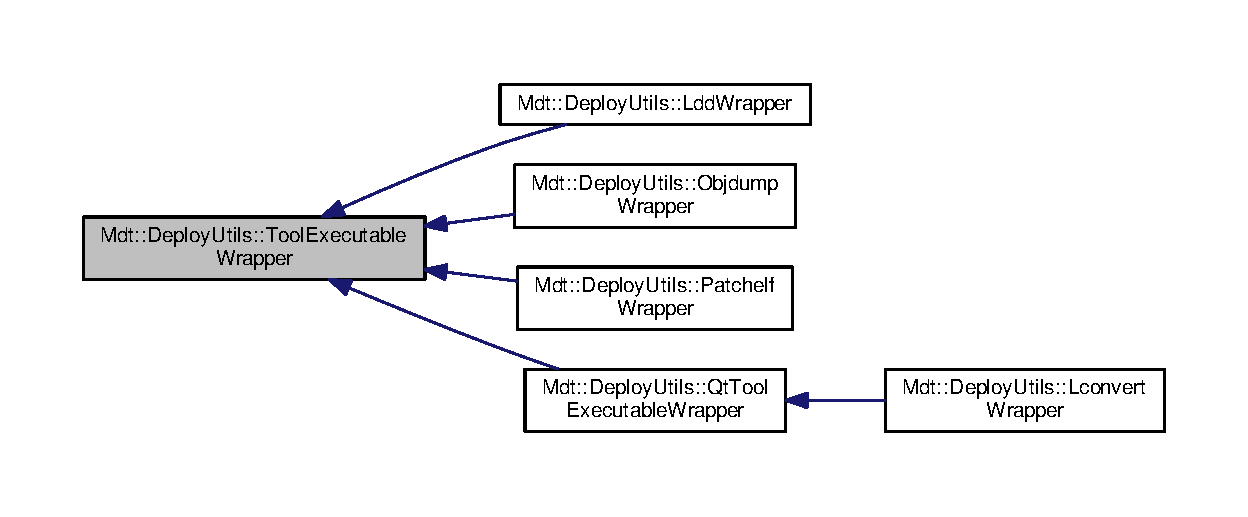
\includegraphics[width=350pt]{class_mdt_1_1_deploy_utils_1_1_tool_executable_wrapper__inherit__graph}
\end{center}
\end{figure}
\subsection*{Public Member Functions}
\begin{DoxyCompactItemize}
\item 
\hyperlink{class_mdt_1_1_deploy_utils_1_1_tool_executable_wrapper_a185d5724b1615df610d30e35070cb414}{Tool\+Executable\+Wrapper} (Q\+Object $\ast$parent=nullptr)\hypertarget{class_mdt_1_1_deploy_utils_1_1_tool_executable_wrapper_a185d5724b1615df610d30e35070cb414}{}\label{class_mdt_1_1_deploy_utils_1_1_tool_executable_wrapper_a185d5724b1615df610d30e35070cb414}

\begin{DoxyCompactList}\small\item\em Constructor. \end{DoxyCompactList}\item 
Q\+String \hyperlink{class_mdt_1_1_deploy_utils_1_1_tool_executable_wrapper_a16c605f652c0ce1df320abc514baa285}{read\+All\+Standard\+Output\+String} ()\hypertarget{class_mdt_1_1_deploy_utils_1_1_tool_executable_wrapper_a16c605f652c0ce1df320abc514baa285}{}\label{class_mdt_1_1_deploy_utils_1_1_tool_executable_wrapper_a16c605f652c0ce1df320abc514baa285}

\begin{DoxyCompactList}\small\item\em Returns all data available from standard output of the channel as string. \end{DoxyCompactList}\item 
Q\+String \hyperlink{class_mdt_1_1_deploy_utils_1_1_tool_executable_wrapper_a4642cfbc69f58af32dc69b4c4619c002}{read\+All\+Standard\+Error\+String} ()\hypertarget{class_mdt_1_1_deploy_utils_1_1_tool_executable_wrapper_a4642cfbc69f58af32dc69b4c4619c002}{}\label{class_mdt_1_1_deploy_utils_1_1_tool_executable_wrapper_a4642cfbc69f58af32dc69b4c4619c002}

\begin{DoxyCompactList}\small\item\em Returns all data available from standard error of the channel as string. \end{DoxyCompactList}\item 
\hyperlink{class_mdt_1_1_error}{Mdt\+::\+Error} \hyperlink{class_mdt_1_1_deploy_utils_1_1_tool_executable_wrapper_a9289a5137a237600e869e077b97259a8}{last\+Error} () const \hypertarget{class_mdt_1_1_deploy_utils_1_1_tool_executable_wrapper_a9289a5137a237600e869e077b97259a8}{}\label{class_mdt_1_1_deploy_utils_1_1_tool_executable_wrapper_a9289a5137a237600e869e077b97259a8}

\begin{DoxyCompactList}\small\item\em Get last error. \end{DoxyCompactList}\end{DoxyCompactItemize}
\subsection*{Protected Member Functions}
\begin{DoxyCompactItemize}
\item 
bool \hyperlink{class_mdt_1_1_deploy_utils_1_1_tool_executable_wrapper_a82d75a83041420d10cb163c084e9828c}{exec} (const Q\+String \&exe\+Name, const Q\+String\+List \&arguments)\hypertarget{class_mdt_1_1_deploy_utils_1_1_tool_executable_wrapper_a82d75a83041420d10cb163c084e9828c}{}\label{class_mdt_1_1_deploy_utils_1_1_tool_executable_wrapper_a82d75a83041420d10cb163c084e9828c}

\begin{DoxyCompactList}\small\item\em Execute a command. \end{DoxyCompactList}\item 
Q\+Process\+::\+Process\+Error \hyperlink{class_mdt_1_1_deploy_utils_1_1_tool_executable_wrapper_a4a94d5952557daed5e91dafb8d4fef85}{last\+Process\+Error} () const \hypertarget{class_mdt_1_1_deploy_utils_1_1_tool_executable_wrapper_a4a94d5952557daed5e91dafb8d4fef85}{}\label{class_mdt_1_1_deploy_utils_1_1_tool_executable_wrapper_a4a94d5952557daed5e91dafb8d4fef85}

\begin{DoxyCompactList}\small\item\em Returns last error from process. \end{DoxyCompactList}\item 
Q\+String\+List \hyperlink{class_mdt_1_1_deploy_utils_1_1_tool_executable_wrapper_ab85cd91b9a6a681624119b316d503e8a}{process\+Arguments} () const \hypertarget{class_mdt_1_1_deploy_utils_1_1_tool_executable_wrapper_ab85cd91b9a6a681624119b316d503e8a}{}\label{class_mdt_1_1_deploy_utils_1_1_tool_executable_wrapper_ab85cd91b9a6a681624119b316d503e8a}

\begin{DoxyCompactList}\small\item\em Get process arguments. \end{DoxyCompactList}\item 
void \hyperlink{class_mdt_1_1_deploy_utils_1_1_tool_executable_wrapper_a13671f8e384893777fd1633dc4984244}{set\+Last\+Error} (const \hyperlink{class_mdt_1_1_error}{Mdt\+::\+Error} \&error)\hypertarget{class_mdt_1_1_deploy_utils_1_1_tool_executable_wrapper_a13671f8e384893777fd1633dc4984244}{}\label{class_mdt_1_1_deploy_utils_1_1_tool_executable_wrapper_a13671f8e384893777fd1633dc4984244}

\begin{DoxyCompactList}\small\item\em Set last error. \end{DoxyCompactList}\end{DoxyCompactItemize}


\subsection{Detailed Description}
Common base class for command line tools (ldd, objdump, ...) 

Definition at line 35 of file Tool\+Executable\+Wrapper.\+h.



The documentation for this class was generated from the following files\+:\begin{DoxyCompactItemize}
\item 
libs/\+Deploy\+Utils\+\_\+\+Core/src/\+Mdt/\+Deploy\+Utils/Tool\+Executable\+Wrapper.\+h\item 
libs/\+Deploy\+Utils\+\_\+\+Core/src/\+Mdt/\+Deploy\+Utils/Tool\+Executable\+Wrapper.\+cpp\end{DoxyCompactItemize}

%--- End generated contents ---

% Index
\backmatter
\newpage
\phantomsection
\clearemptydoublepage
\addcontentsline{toc}{chapter}{Index}
\printindex

\end{document}
